% SPDX-License-Identifier: CC-BY-4.0
% Copyright (C) 2026 Fabian Januszewski, Abhijit (the Langlandscape team)
% Modular SOURCE of the Mathathon submission report of team Langlandscape.
% Build (modular draft): cd mathematics/submission/src && latexmk -pdf report-src.tex   (bibtex, amsalpha)
% The single self-contained report.tex is produced from this file by ../tools/flatten.py (it inlines every \input,
% decides the \IfFileExists switches, strips comments and inlines the bibliography as thebibliography).
% Rules: plain \cite only; no images; every figure has a caption of >= 12 words describing it; no person, machine or
% user names outside the title block (\title ... \maketitle), which is stripped for the anonymous review.
\documentclass[11pt]{article}
% SPDX-License-Identifier: CC-BY-4.0
% Copyright (C) 2026 Fabian Januszewski, Abhijit (the Langlandscape team)
% Macros of the submission report: mathematics/preamble.tex without biblatex (bibtex + amsalpha instead),
% plus the few chapter-level macros and a tcolorbox-free version of the quoted-statement environment.
% Packages: standard LaTeX/AMS only (the flattened report.tex must compile with a plain TeX Live).
\usepackage[T1]{fontenc}
\usepackage[utf8]{inputenc}
\usepackage{lmodern}
\usepackage[a4paper,margin=2.5cm]{geometry}
\usepackage{amsmath,amssymb,amsthm,mathtools}
\usepackage{booktabs,array,longtable}
\usepackage{enumitem}
\usepackage{xcolor}
\usepackage[colorlinks=true,linkcolor=blue!50!black,citecolor=green!40!black,urlcolor=blue!50!black]{hyperref}
\setlist{itemsep=2pt,topsep=3pt}
\setlength{\emergencystretch}{3em}

%---------------------------------------------------------------- theorem environments
\theoremstyle{plain}
\newtheorem{theorem}{Theorem}[section]
\newtheorem{proposition}[theorem]{Proposition}
\newtheorem{lemma}[theorem]{Lemma}
\newtheorem{corollary}[theorem]{Corollary}
\newtheorem{conjecture}[theorem]{Conjecture}
\theoremstyle{definition}
\newtheorem{definition}[theorem]{Definition}
\newtheorem{hypothesis}[theorem]{Hypothesis}
\newtheorem{interface}[theorem]{Interface}
\newtheorem{example}[theorem]{Example}
\newtheorem{testcase}[theorem]{Test case}
\theoremstyle{remark}
\newtheorem{remark}[theorem]{Remark}

%---------------------------------------------------------------- status markers
% Usage: \status{cited}, \status{to prove}, \status{conjectural}, \status{known}, ...
\newcommand{\status}[1]{\textup{\textsf{[#1]}}}
\newcommand{\stknown}{\status{known}}          % standard / textbook, reference given
\newcommand{\stcited}{\status{cited}}          % taken from literature, precise pointer given
\newcommand{\sttoprove}{\status{to prove}}     % we must write the proof
\newcommand{\stproved}{\status{proved}}        % proof written in this plan / seed
\newcommand{\stpmc}{\status{proved modulo cited}}
\newcommand{\stsketch}{\status{sketched}}
\newcommand{\stexp}{\status{expected}}
\newcommand{\stconj}{\status{conjectural}}
\newcommand{\sthyp}{\status{hypothesis}}
\newcommand{\stopen}{\status{open}}
\newcommand{\stcomp}{\status{computed}}
\newcommand{\stformal}{\status{formalized}}    % exists in Lean (give declaration name)
% literature pointer: \lit{file-stem}{Thm 4.5, p.~12}

\newcommand{\litund}{\char`\_\penalty0\hskip0pt\relax}
\newcommand{\lit}[2]{\textup{(\pathtt{literature/#1}, #2)}}

%---------------------------------------------------------------- number systems
\newcommand{\Q}{\mathbb{Q}}\newcommand{\Z}{\mathbb{Z}}\newcommand{\R}{\mathbb{R}}\newcommand{\C}{\mathbb{C}}
\newcommand{\F}{\mathbb{F}}\newcommand{\A}{\mathbb{A}}
\newcommand{\Zp}{\mathbb{Z}_p}\newcommand{\Qp}{\mathbb{Q}_p}\newcommand{\Zq}{\mathbb{Z}_q}\newcommand{\Qq}{\mathbb{Q}_q}
\newcommand{\Zhat}{\hat{\mathbb{Z}}}\newcommand{\Qhat}{\hat{\mathbb{Q}}}
\newcommand{\cO}{\mathcal{O}}\newcommand{\cOE}{\mathcal{O}_E}

%---------------------------------------------------------------- groups, algebras
\newcommand{\GL}{\mathrm{GL}}\newcommand{\SL}{\mathrm{SL}}\newcommand{\PGL}{\mathrm{PGL}}
\newcommand{\Nrd}{\mathrm{Nrd}}\newcommand{\Trd}{\mathrm{Trd}}\newcommand{\Sym}{\mathrm{Sym}}
\newcommand{\JL}{\mathrm{JL}}\newcommand{\ord}{\mathrm{ord}}\newcommand{\Iw}{\mathrm{Iw}}
\newcommand{\Hb}{\mathfrak{H}}
\newcommand{\Bd}{B_D}                       % definite quaternion algebra over Q of discriminant D
\newcommand{\Bhat}{\hat{B}}                 % B tensor finite adeles
\newcommand{\XB}[1]{X_B(#1)}                % class set B^x \ \hat B^x / U
\newcommand{\XBq}[1]{X_{B_q}(#1)}
\newcommand{\Uzero}[1]{U_0(#1)}\newcommand{\Uone}[1]{U_1(#1)}
\newcommand{\Brandt}[2]{M(#1;#2)}           % Brandt module M(U;V)
\newcommand{\Vk}{V_k}                       % Sym^{k-2}(Z_p^2)
\newcommand{\GU}{\Gamma_U}                  % norm-one S-arithmetic group O_U[1/q]^1

%---------------------------------------------------------------- trees and graphs
\newcommand{\cT}{\mathcal{T}}               % Bruhat--Tits tree T_q
\newcommand{\G}{\mathbb{G}}                 % weighted graph / quotient graph of groups
\newcommand{\GDR}{\G^{\mathrm{DR}}}
\newcommand{\Phicomb}{\Phi^{\mathrm{comb}}}
\newcommand{\Xcomb}{X^{\mathrm{comb}}}
\newcommand{\cX}{\mathcal{X}}               % tree model of indefinite stage
\newcommand{\quot}{\backslash\backslash}    % quotient graph of groups

%---------------------------------------------------------------- Hecke, Hida
\newcommand{\T}{\mathbb{T}}\newcommand{\m}{\mathfrak{m}}
\newcommand{\Lam}{\Lambda}
\newcommand{\cM}{\mathcal{M}}
\newcommand{\Mord}{\cM^{\mathrm{ord}}_B}
\newcommand{\Xord}{\cX^{\mathrm{ord}}}
\newcommand{\Tord}{\mathcal{T}^{\mathrm{ord}}} % Hida's ordinary Tate module
\newcommand{\fa}{\mathfrak{a}}\newcommand{\fb}{\mathfrak{b}}
\newcommand{\cc}{\mathfrak{c}}\newcommand{\tq}{\mathfrak{t}}

%---------------------------------------------------------------- hypotheses
\newcommand{\HypX}{\mathrm{Hyp.X}}
\newcommand{\HypXchar}{\mathrm{Hyp.X.char}}
\newcommand{\HypXgal}{\mathrm{Hyp.X.gal}}
\newcommand{\HypXiso}{\mathrm{Hyp.X}^{\mathrm{iso}}}

%---------------------------------------------------------------- operators
\DeclareMathOperator{\Hom}{Hom}\DeclareMathOperator{\coker}{coker}\DeclareMathOperator{\End}{End}
\DeclareMathOperator{\Ann}{Ann}\DeclareMathOperator{\rk}{rk}\DeclareMathOperator{\Stab}{Stab}
\DeclareMathOperator{\tr}{tr}\DeclareMathOperator{\Jac}{Jac}\DeclareMathOperator{\Fitt}{Fitt}

%---------------------------------------------------------------- macros shared by several stages
% (moved here from the stage files; the stages' \providecommand lines are then no-ops)
\providecommand{\Tpath}[1]{\pathtt{#1}}
\providecommand{\BG}{\mathrm{BG}}          % bipartite Brandt graph of (U,q)
\providecommand{\Xone}{X^1_B}              % norm-one class set
\providecommand{\HypSA}{\mathrm{Hyp.SA}}   % strong approximation hypothesis
\providecommand{\HypHS}{\mathrm{Hyp.HS}}   % Hasse--Schilling norm hypothesis
\providecommand{\NUp}{N_{U_p}}             % the U_p normalisation fixed in stage 01
\providecommand{\Kp}[1]{K_{#1}}            % K_s = U_1(p^s)_p
\providecommand{\Kpp}[1]{K'_{#1}}          % K'_s = U_1(p^s)_p \cap U_0(p^{s+1})_p
\providecommand{\TordB}{\T^{\mathrm{ord}}_B}   % ordinary definite Hecke algebra (NOT \Tord)
\providecommand{\cH}{\mathcal{H}}          % abstract Hecke algebra H_s of Hyp.X
\providecommand{\Xq}{X_q}                  % character group at q
\providecommand{\Ros}{\mathsf{Ros}}          % Rosati dual (distinct from \vee = dual variety/morphism)
\providecommand{\Frob}{\mathrm{Frob}}
\providecommand{\St}{\mathrm{St}}          % Steinberg representation

%---------------------------------------------------------------- provisional changes (global Fable seam audit)
% \provisional{Fk/Dn: what changed; before: ...} marks a change made provisionally after
% audits/global-fable-seam.md, pending Fabian's review (see audits/global-fable-resolution.md).
% Revert a change by restoring the "before" text and deleting the note.
\providecommand{\provisional}[1]{\textcolor{orange!75!black}{\textsf{\small[provisional: #1]}}}

%---------------------------------------------------------------- Lean and status markers (mathematics/ only)
% \lean{Langlandscape.Name}: cross-reference to a formalized declaration (typeset in small \texttt).
% \pathtt{...}: typewriter path or Lean name with line-break points after /, ., \_ (round R5; no external files).
\ExplSyntaxOn
\tl_new:N \l__llpath_tl
\cs_new_protected:Npn \__llpath_typeset:n #1
  {
    \tl_set:Nn \l__llpath_tl {#1}
    \tl_replace_all:Nnn \l__llpath_tl { / } { /\penalty\exhyphenpenalty\hskip0pt\relax }
    \tl_replace_all:Nnn \l__llpath_tl { . } { .\penalty\exhyphenpenalty\hskip0pt\relax }
    \tl_replace_all:Nnn \l__llpath_tl { \_ } { \_\penalty\exhyphenpenalty\hskip0pt\relax }
    \tl_replace_all:Nnn \l__llpath_tl { - } { -\penalty\exhyphenpenalty\hskip0pt\relax }
    \tl_replace_all:Nnn \l__llpath_tl { : } { :\penalty\exhyphenpenalty\hskip0pt\relax }
    \texttt { \tl_use:N \l__llpath_tl }
  }
\NewDocumentCommand \pathtt { m } { \__llpath_typeset:n {#1} }
\ExplSyntaxOff
\newcommand{\lean}[1]{\textup{\small(Lean: \pathtt{#1})}}
% \leanplanned: the result is planned for Lean but not yet formalized.
\newcommand{\leanplanned}{\textup{\small(Lean: planned)}}
% \stformalized: status marker, exists in Lean (same meaning as \stformal; give \lean{} next to it).
\newcommand{\stformalized}{\status{formalized}}

%---------------------------------------------------------------- additions for the submission report
\usepackage{tikz}
\usetikzlibrary{arrows.meta,positioning}
\makeatletter
\providecommand{\sfref}[1]{\@ifundefined{r@#1}{\texttt{#1}}{\ref{#1}}}
\makeatother
\providecommand{\stformalized}{\status{formalized}}
% Placeholder for facts the team still has to supply (filled in by the global master before submission).
% \newcommand{\TODOFACT}[1]{\textbf{[TODO: #1]}}  (placeholder macro, no longer used)
\newcommand{\PublicCommitHash}{9f1de427748a0e5536a8f7163b6a7ff71e2bf8f8}
% Pointer into the full mathematical text (not part of this file): (main.pdf, Thm 10.2).
\newcommand{\mainpdf}{\pathtt{mathematics/main.pdf}}
% Loose lines rather than overfull ones (round R5).
\setlength{\emergencystretch}{3em}
\newcommand{\mainref}[1]{\textup{(main.pdf, #1)}}
\newcommand{\res}[1]{{\small\nolinkurl{code/results/#1}}}
% Proof outline of a quoted statement: \begin{outline} ... \end{outline}
\newenvironment{outline}{\par\smallskip\noindent\textit{Proof outline.}\ }{\par\medskip}
% Verbatim-quoted result from the chapters (a plain-text replacement of the boxed version in
% mathematics/final-report/): {kind}{number in main.pdf}{page}{label}{title}{source file}.
% Each quoted block is followed in the source by an explicit \label{rpt:<chapter label>} (inserted by
% tools/add_rpt_labels.py), whose \ref prints the main.pdf number (#2); the flattener
% rewrites \ref{<chapter label>} to \ref{rpt:<chapter label>} so that every referenced result is inside the report.
\makeatletter
\newenvironment{quoted}[6]{%
  \if@noskipsec\leavevmode\par\fi% a pending run-in \paragraph heading gets its own line
  \par\medskip\noindent\rule{\linewidth}{0.4pt}\par\nopagebreak
  \phantomsection\def\@currentlabel{#2}%
  \noindent\textbf{#1 #2}\ifx\relax#5\relax\else\ (#5)\fi\par\nopagebreak
  \noindent{\scriptsize\raggedright Quoted verbatim from main.pdf, p.~#3 (label \pathtt{#4}; source \pathtt{mathematics/#6}).\par}\nopagebreak\smallskip
  \small\sloppy}{\par\noindent\rule{\linewidth}{0.4pt}\par\medskip}
\makeatother
% Unicode that may occur in quoted Lean signatures (pdflatex).
\DeclareUnicodeCharacter{2200}{\ensuremath{\forall}}
\DeclareUnicodeCharacter{2192}{\ensuremath{\to}}
\DeclareUnicodeCharacter{03C1}{\ensuremath{\rho}}
\DeclareUnicodeCharacter{03C6}{\ensuremath{\varphi}}
\DeclareUnicodeCharacter{211A}{\ensuremath{\mathbb{Q}}}
\DeclareUnicodeCharacter{03B3}{\ensuremath{\gamma}}
\DeclareUnicodeCharacter{03C0}{\ensuremath{\pi}}
\DeclareUnicodeCharacter{039B}{\ensuremath{\Lambda}}
\DeclareUnicodeCharacter{2203}{\ensuremath{\exists}}
\DeclareUnicodeCharacter{02E3}{\ensuremath{^{\times}}}
\DeclareUnicodeCharacter{2227}{\ensuremath{\wedge}}
\DeclareUnicodeCharacter{2113}{\ensuremath{\ell}}
\DeclareUnicodeCharacter{2265}{\ensuremath{\geq}}
\DeclareUnicodeCharacter{2261}{\ensuremath{\equiv}}
% \rptnum{main.pdf number}\label{rpt:<chapter label>}: mark a paraphrased (not verbatim) copy of a chapter result or
% definition in the report, so that \ref{rpt:<chapter label>} resolves to it (prints the main.pdf number). The \label must
% be written out literally (the flattener looks for it).
\makeatletter
\newcommand{\rptnum}[1]{\phantomsection\def\@currentlabel{#1}}
\makeatother
% Revision notes inside quoted chapter statements (the chapters' \provisional{...} notes, renamed for the report): they
% record a change made after an internal audit and the previous wording; the decisions they mention have been taken.
\newcommand{\revnote}[1]{\textup{\textsf{\small[revision note: #1]}}}
% Lean name of the Hyp.BrandtStabFree discharge (impl/brandtstab-discharge).
\providecommand{\BSFdischargeName}{\pathtt{Hyp.brandtStabFree\_holds}}

% SPDX-License-Identifier: CC-BY-4.0
% Copyright (C) 2026 Fabian Januszewski, Abhijit (the Langlandscape team)
% Macros for Appendix A (the hypotheses report as text): a copy of mathematics/report/hyp-preamble.tex without
% tcolorbox, colortbl and placeins (the boxed environments become plain titled blocks). Loaded after macros.tex.
\usetikzlibrary{shapes.geometric,fit,calc,backgrounds}

% Okabe--Ito palette (colour-blind safe); every status also has a distinct line style, and the appendix
% introduction describes both figures in words.
\definecolor{oiBlue}{HTML}{0072B2}
\definecolor{oiGreen}{HTML}{009E73}
\definecolor{oiOrange}{HTML}{E69F00}
\definecolor{oiVerm}{HTML}{D55E00}
\definecolor{oiPurple}{HTML}{CC79A7}
\definecolor{oiSky}{HTML}{56B4E9}
\definecolor{oiGrey}{HTML}{6E6E6E}

% Kind markers (the text label LIT, DIS, INF, OOS, CON, PLN carries the meaning; the box is decoration).
\newcommand{\kindbox}[2]{\tikz[baseline=-0.6ex]\node[draw=#1,fill=#1!25,line width=0.8pt,inner sep=1.6pt,
  rounded corners=1pt,font=\scriptsize\sffamily]{#2};}
\newcommand{\kindlit}{\kindbox{oiBlue}{LIT}}
\newcommand{\kinddis}{\kindbox{oiGreen}{DIS}}
\newcommand{\kindinfra}{\kindbox{oiOrange}{INF}}
\newcommand{\kindoos}{\kindbox{oiVerm}{OOS}}
\newcommand{\kindcond}{\kindbox{oiPurple}{CON}}
\newcommand{\kindplan}{\tikz[baseline=-0.6ex]\node[draw=oiSky!70!black,dashed,fill=oiSky!15,line width=0.8pt,
  inner sep=1.6pt,rounded corners=1pt,font=\scriptsize\sffamily]{PLN};}

% Lean names and paths: typewriter, breakable after '/' and '.'.
\makeatletter
\begingroup
  \catcode`\/=\active \catcode`\.=\active
  \gdef\lname@slash{\char`\/\penalty\exhyphenpenalty\hskip0pt\relax}
  \gdef\lname@dot{\char`\.\penalty\exhyphenpenalty\hskip0pt\relax}
  \gdef\lname@activate{\catcode`\/=\active \catcode`\.=\active \let/\lname@slash \let.\lname@dot
    \def\_{\textunderscore\penalty500\hskip0pt\relax}}
\endgroup
\DeclareRobustCommand{\lname}{\begingroup\ttfamily\lname@activate\lname@aux}
\newcommand{\lname@aux}[1]{#1\endgroup}
\makeatother
\providecommand{\brk}{\penalty0\hskip0pt\relax}

% One entry per hypothesis: \begin{hypentry}{ShortName}{\kindlit}{S02-L4a} ... \end{hypentry}
\newenvironment{hypentry}[3]
  {\par\medskip\noindent\rule{\linewidth}{0.3pt}\par\nopagebreak
   \noindent\texttt{#1}\hfill #2\ \ \textsf{\small introduced #3}\par\nopagebreak
   \small\rightskip=0pt plus 4em\relax
   \begin{description}[leftmargin=0pt,labelsep=0.4em,itemsep=1.5pt,topsep=2pt,font=\normalfont\bfseries]}
  {\end{description}\par\noindent\rule{\linewidth}{0.3pt}\par\medskip}

% A titled reading guide.
\newenvironment{readbox}[1][]
  {\par\medskip\noindent\textbf{#1}\par\nopagebreak\begin{quote}}
  {\end{quote}\par\medskip}

% SPDX-License-Identifier: CC-BY-4.0
% Copyright (C) 2026 Fabian Januszewski, Abhijit (the Langlandscape team)
% Single source of the Lean status numbers used in the submission report (copied from final-report/counts.tex). Update ONLY here.
\newcommand{\NumHypRegistered}{29}      % registered hypotheses
\newcommand{\NumHypDischarged}{3}       % discharged
\newcommand{\NumHypCondDischarged}{1}   % conditionally discharged
\newcommand{\HypDischargedNames}{\texttt{PadicOrdDecomp}, \texttt{RamNrdSurj}, \texttt{BrandtStabFree}}
\newcommand{\HypCondDischargedNames}{\texttt{ResidualBurnside}, from absolute irreducibility}
\newcommand{\NumHypOpen}{\number\numexpr\NumHypRegistered-\NumHypDischarged-\NumHypCondDischarged\relax}
\newcommand{\NumHypRows}{\number\numexpr\NumHypRegistered-1\relax}   % Langlandscape.Hyp.* rows (the import's EichlerMass is the extra one)
\newcommand{\NumHypTableRows}{26}       % rows of the summary table of the hypotheses report
\newcommand{\GateAudited}{955}          % final gate bsf-gate-1 (from scratch, Lean tree c70ef3a9); previous: subl-gate-1 (tree 28d2b091) 950, ramnrd-final-2 (2323a252) 840
\newcommand{\NumAuditedRows}{\GateAudited}  % rows of Audit/PrintAxioms.lean (all gated)

\hypersetup{pdftitle={The definite Jacquet-Langlands correspondence over Q, integral and Lambda-adic},pdfauthor={},pdfsubject={Mathathon submission report}}
\numberwithin{equation}{section}
\setcounter{tocdepth}{2}

% Parallel inputs: the Lean table and discipline paragraph (branch final/leantable). If a file is not (yet) present, a
% temporary stub from src/stubs/ is used; the flattener decides the switch. Chapter s00 (mathematics/chapters/s00/) supplies
% Sections 1-5 and the head of Section 6 with its own \section headings; its \ref's to chapter labels are rewritten by
% the flattener into main.pdf numbers (in this modular build they print as ??).

%=============================================================================== TITLE BLOCK (stripped for review)
% The title block is the ONLY place naming persons, affiliations and the repository. The acknowledgments wording
% (mathematics/acknowledgments.tex, fixed) names a team member; it is therefore placed here, as a \thanks note, so
% that the body after \maketitle stays anonymous.
\title{The definite Jacquet--Langlands correspondence over $\Q$, integral and $\Lambda$-adic:\\
a Bruhat--Tits tree route, a Lean~4 formalization and computations\\[4pt]
\large Submission report, Caltech $\times$ SAIR Mathathon 2026}
\author{M.Sc. Abhijit Aryampilly Jayanthan\thanks{Institute of Mathematics, Department EIM, Paderborn University.}
  \and Prof.\ Dr.\ Fabian Januszewski\thanks{Institute of Mathematics, Department EIM, Paderborn University.}
  \thanks{\textbf{Acknowledgments.} We gratefully acknowledge support from an NVIDIA Academic Grant Program award to Fabian Januszewski (CUDA-GNFS project), which provided two NVIDIA RTX PRO 6000 Max-Q Workstation Edition GPUs used for the HACS computations, and from the Deutsche Forschungsgemeinschaft (DFG, German Research Foundation) -- SFB-TRR 358/1 2023 -- 491392403. We thank the organizers of the Caltech $\times$ SAIR Mathathon 2026 for compute credits on the Open Math Model platform (\url{https://os.openmathmodel.org/}), which were used in this project (the opencode models Muse Spark Open and Mistral Large 4).}}
\date{Track: Algebra/Number Theory\\ Repository: \url{https://github.com/drjanosch42/Langlandscape-Mathathon}, commit \texttt{\PublicCommitHash}\thanks{Content commit of the public repository; the next commit changes only the line defining this hash (in the report sources and the flattened report) and its PDF.}\\ 15 November 2026}
\begin{document}
\maketitle
%=============================================================================== END OF TITLE BLOCK

% SPDX-License-Identifier: CC-BY-4.0
% Copyright (C) 2026 Fabian Januszewski, Abhijit (the Langlandscape team)
\begin{abstract}% SPDX-License-Identifier: CC-BY-4.0
% Copyright (C) 2026 the Langlandscape team
% Short abstract (text only, no abstract environment); shared by submission/src/abstract.tex and article.tex.
% \GateAudited comes from submission/src/counts.tex; the literal fallback 950 is used where it is not defined.
We study the Jacquet--Langlands correspondence between a \emph{definite} quaternion algebra $B$ over $\Q$ and $\GL_2$,
seeking it as an integral, Hecke-equivariant \emph{map} rather than a trace identity. Following Ihara and Serre, we realise the
definite side on Bruhat--Tits tree quotients, bridged to $\GL_2$ by Ribet's exact sequence. For discriminant
$D=q$ our main result is an integral \emph{defect formula}: for a $q$-new Hida family, the ratio of the two congruence ideals
is the old/new congruence ideal, equal to the local Tamagawa ideal at $q$. It is proved modulo cited results under
explicit hypotheses (open for $q\equiv-1\bmod p$ outside the level conditions (Lev)). In the first case ($D=q$, weight~$2$) our route reproves classical Jacquet--Langlands modulo cited geometry; elsewhere Jacquet--Langlands is cited. In Lean~4, \ifdefined\GateAudited\GateAudited\else 950\fi{} audited declarations use only the standard
axioms, with registered hypotheses as explicit arguments. Computations: Python/PARI and HACS. We also correct one sign in the
literature.
\end{abstract}


\setcounter{tocdepth}{1}
\tableofcontents

% Sections 1-5 and the head of Section 6 come from chapter s00 (each file starts with its own \section).
% SPDX-License-Identifier: CC-BY-4.0
% Copyright (C) 2026 the Langlandscape team
% Status-tag legend (round R5). Shared: start of chapter s00 (main.tex), after the abstract of the article and of the
% submission report. No \input; uses only the status macros of preamble.tex / submission/src/macros.tex.
\begin{sloppypar}
\noindent\textbf{Status tags.} Every result carries its status as a tag in brackets, printed exactly as follows.
\begin{itemize}\setlength{\itemsep}{0pt}
\item \stproved: the proof is written out in our chapters.
\item \stpmc: proved, using the named cited results as black boxes; \status{proved modulo cited geometry}: the same, where
  the cited inputs are the geometric results named there (Deligne--Rapoport, Deuring, Grothendieck's character group).
\item \stcited: taken from the literature with a precise pointer, not reproved; \stknown: standard or textbook, with a
  reference.
\item \status{definition}: a definition, nothing to prove; \sthyp: a named hypothesis, assumed only where stated and never
  claimed.
\item \stcomp: checked by machine computation over the stated range; a computation is never part of a proof.
\item \stformal: a Lean~4 declaration with this content compiles with the standard axioms only, named next to it as
  \textup{\small(Lean: \dots)}; \emph{formalized modulo $H$} (\emph{Lean-conditional}): the same, with the registered
  hypotheses $H$ as explicit arguments; \textup{\small(Lean: planned)}: not yet formalized. In the claims table of the
  submission report, \emph{Lean-verified} means formalized without qualifier, with no difference recorded.
\item \stsketch, \stexp, \stconj, \stopen, \sttoprove: no proof is claimed (a sketch is given; expected to hold; a
  conjecture; an open question; a proof still to be written).
\item Notes on changes after internal audits are printed as \textup{\textsf{\small[provisional: \dots]}} in the chapters and
  as \textup{\textsf{\small[revision note: \dots]}} in the submission report.
\end{itemize}
\end{sloppypar}

\newcommand{\sOOsummary}{% SPDX-License-Identifier: CC-BY-4.0
% Copyright (C) 2026 the Langlandscape team
% Detailed summary (the former long abstract, unchanged in content); report only, via \sOOsummary at the start of s00/motivation.
\paragraph{Summary of results.}
We study the Jacquet--Langlands correspondence between a \emph{definite} quaternion algebra $B$ over $\Q$ and $\GL_2$ and ask
for it as an integral, Hecke-equivariant and computable \emph{map} rather than a trace identity. Following Ihara and Serre we
realise the definite side by quotients of the Bruhat--Tits tree of $\GL_2(\Q_q)$ by $S$-arithmetic quaternionic groups, and build
the route in six stages: class sets, Brandt modules and Hecke operators; tree quotients and the Brandt graph; the definite
Ribet sequence and the definite Ihara lemma as statements about weighted graphs (with Mazur's component group
$\Z/\mathrm{num}\frac{q-1}{12}$, where $\mathrm{num}\frac{q-1}{12}$ is the numerator of $\frac{q-1}{12}$ in lowest terms, recovered combinatorially); the ordinary $\Lambda$-adic passage up the $p$-power tower; a single
comparison hypothesis $\HypX$ that isolates all geometry; and, for discriminant $D=q$, an integral \emph{defect formula}: for a
$q$-new Hida branch $F$ the ratio of the congruence ideals on the two sides is the old/new congruence ideal $\cc_q(F)$, and
$\cc_q(F)$ equals the local Tamagawa ideal $\tq_q(F)$. The defect formula is proved modulo cited results (Hida, Hsieh, Kim--Ota)
under the explicit standing hypotheses of \S\ref{ss:s00-H} (among them $p\ge5$, $p\nmid\varphi(qM)$, a non-Eisenstein maximal
ideal, residual absolute irreducibility and $p$-distinguishedness, the existence of a suitable arithmetic point, and either
$q\not\equiv-1\bmod p$, or $\bar\rho$ ramified at $q$, or one of the level conditions (Lev)); for $q\equiv-1\bmod p$ outside (Lev)
($N(\bar\rho)>1$, or non-squarefree $M$) it is open. In the first case ($D=q$, weight~$2$) our route reproves classical Jacquet--Langlands modulo cited geometry
(Ribet's argument, in our combinatorial form on the tree; \S\ref{ss:s00-whycited}); elsewhere Jacquet--Langlands is cited (\S\ref{ss:s00-whycited}). A large part is formalized in Lean~4 (\GateAudited{} audited
declarations, standard axioms only, no \texttt{sorry} in any of them; every cited or not yet formalized input is an explicit argument: one of \NumHypRegistered{} registered hypotheses, of which
\NumHypDischarged{} are discharged, or a stated premise such as the connectivity of the Brandt graph; several statements are about
abstract data), and the
statements were checked numerically with Python/PARI and the HACS engine. Every claim below carries its status, exactly as in
our chapters: proved (on paper, with a proof outline here), proved modulo cited results, Lean-verified, Lean-conditional on named
hypotheses, computed (with range), cited, or conjectural/open. We also record one sign correction to the literature.
}% detailed summary at the start of s00/motivation (report only)
% SPDX-License-Identifier: CC-BY-4.0
% Copyright (C) 2026 Fabian Januszewski, Abhijit (the Langlandscape team)
% Stage 00 (introduction), part 1: the problem statement and our motivation. No \input; reusable in the report.
\section{The problem and our motivation}\label{ss:s00-motivation}
\ifdefined\sOOsummary\sOOsummary\fi

\subsection{The problem}
The problem we were set reads, verbatim:
\begin{quote}
``The Jacquet--Langlands correspondence, established by Herv\'e Jacquet and Robert Langlands in 1970, is a foundational result
in number theory and representation theory. It links automorphic representations of GL(2) with those of the multiplicative
group of a quaternion algebra, matching representations that share the same local data and L-functions. As one of the
earliest proven cases of Langlands functoriality, it became an essential tool in modern arithmetic, including work leading to
the proof of Fermat's Last Theorem.''
\end{quote}
with the references \cite{JL} (H.~Jacquet and R.~P.~Langlands, \emph{Automorphic Forms on GL(2)}, Lecture Notes in Math.~114,
Springer 1970, doi:10.1007/BFb0058988) and \cite[Ch.~8]{Bergeron16} (N.~Bergeron, \emph{The Spectrum of Hyperbolic Surfaces},
Universitext, Springer 2016, Chapter~8, doi:10.1007/978-3-319-27666-3\_8). The desired outcome was stated as:
\begin{quote}
``A new approach to the construction of the Jacquet-Langlands functorial transfer and the characterization of its image. If
early attempts to a new approach bear no fruit, we could aim at a LEAN formalization of the trace formula proof, with an
accompanying human-readable mathematically consistent writeup.''
\end{quote}
We took the first alternative. In the first case ($D=q$, weight~$2$, $\Gamma_0$-type level) our route reproves classical JL
modulo the cited geometry (\S\ref{ss:s00-whycited}); beyond $D=q$ it invokes the correspondence: classical, $p$-adic and
$\Lambda$-adic JL are \emph{cited} (Thm.~\ref{thm:s01-JLclassical}, Thm.~\ref{thm:s01-chenevier}, Thm.~\ref{thm:s01-lambdaJL}, all
\stcited). What we built is an \emph{integral, combinatorial} approach to the transfer on the definite side, which isolates
the one geometric input in a single named hypothesis, and an integral theorem on the image: the defect formula of stage~06
(\S\ref{ss:s00-outline}). The narrative of this chapter is: classical JL (an equality of spectra, a trace identity)
$\to$ the hope, an integral Hecke-equivariant map with properties (a)--(e) (\S\ref{ss:s00-hope}) $\to$ Ribet's exact sequence, which
realises the hope in the first case $D=q$, weight~$2$, $\Gamma_0(qM)$ (\S\ref{ss:s00-ribet}), and its combinatorial form on the
Bruhat--Tits tree $\to$ what we did (\S\S\ref{ss:s00-question}--\ref{ss:s00-newknown}).

\subsection{Motivation: congruences and integral structure}\label{ss:s00-why}
Over $\C$ the correspondence is a bijection of automorphic representations, and its shadow on traces is an identity of trace
formulas. Arithmetic needs more: it needs the correspondence on \emph{lattices}, because congruences between eigenforms are
properties of $\Z$- or $\Zp$-structures and are invisible over a field. We kept the following picture in mind; every point
is made precise later, with the status stated there.
\begin{enumerate}[label=(M\arabic*)]
\item \emph{JL carries congruences from the quaternionic side to $\GL_2$.} Two congruent quaternionic Hecke eigensystems give
  congruent $D$-new eigensystems for $\GL_2$, away from $D$ and, at $\ell\mid D$, through the matching $U_\ell\mapsto+\Pi_\ell$
  of the $\Lambda$-adic Hecke JL in our normalisation. This is a consequence of the surjection of Hecke algebras in
  Thm.~\ref{thm:s01-lambdaJL} (\stcited). The sign is fixed in stage~05, Prop.~\ref{prop:s05-sign}: \stpmc{} at $\Gamma_0$-level, and
  at $\Gamma_1$-level \stpmc{} given (X1) and the model decision FD1.
\item \emph{The converse fails.} At $\ell\mid D$ the image of JL consists of forms that are special (Steinberg type) at $\ell$, while
  $B_\ell^\times$ sees only one-dimensional representations there. The quaternionic side therefore sees only $D$-new forms. A
  congruence between a $D$-new form and a form that is old or unramified principal series at $\ell$ (level raising) has no
  quaternionic counterpart: it is not killed, it simply has nowhere to live on the $B$-side. (\stknown; level raising:
  \cite{Ri84}, cited as in stage~06.)
\item \emph{The missing congruences are measured by a defect.} For $D=q$ and a $q$-new Hida branch $F$, stage~06 identifies the
  defect $(h_F)=\eta_F(\eta^B_F)^{-1}$ between the congruence ideals on the two sides with the old/new congruence ideal
  $\cc_q(F)$ and the Tamagawa ideal $\tq_q(F)$ (Thm.~\ref{thm:s06-defect}, \stpmc{} under the standing hypotheses; \S\ref{ss:s00-outline}).
  This is the integral form of ``JL loses exactly the level-raising congruences at $q$''.
\item \emph{An integral comparison map sees this as a cokernel.} For $D=q$ such a map exists classically: Ribet's exact
  sequence (\S\ref{ss:s00-ribet}, \stcited), whose definite side we reprove on the Bruhat--Tits tree. For maps of this kind, the
  sub-versus-quotient comparison of $q$-new lattices has cokernel $(\T/(\fa+\fb))^{\oplus r}$, the congruence module
  (Prop.~\ref{prop:s05-subquot}, \stproved, \stformal); so ``congruences are obstructions'' becomes the precise statement
  ``cokernel $=$ congruence module'' (\S\ref{ss:s00-map}).
\end{enumerate}

% SPDX-License-Identifier: CC-BY-4.0
% Copyright (C) 2026 the Langlandscape team
% Stage 00 (introduction): where classical JL is reproved (first case, modulo cited geometry) and where it is cited. No \input; shared by main.tex and the submission report.
\subsection{Classical JL: first case modulo cited geometry; cited in general}\label{ss:s00-whycited}
Item (a) of the question (\S\ref{ss:s00-hope}; item (iii) of the seed) asks that the integral map recover classical JL over $\C$, and
the desired outcome of the problem was ``a new approach to the construction of the Jacquet--Langlands functorial transfer and the
characterization of its image''. Classical JL enters our chapters as a cited input (Thm.~\ref{thm:s01-JLclassical}, \stcited); in
the first case our route also reproves it, modulo cited geometry. In detail:

\emph{Which alternative we took.} The problem offered a new approach or, failing that, a Lean formalization of the trace-formula
proof. We took the new approach and aimed it at the integral and arithmetic content that the trace formula does not see: maps
between lattices, their cokernels as congruence modules, and the defect, which is our integral form of ``the characterization of
its image'' (\S\ref{ss:s00-why}, \S\ref{ss:s00-map}).

\emph{What the route recovers.} In the first case, $D=q$, weight~$2$ and level $\Gamma_0(qM)$, Ribet's sequence is an explicit,
integral, Hecke-equivariant comparison $\Xq(J_0(qM'))\cong\Z[\XBq{\Uzero{M'}}]^0$ (Thm.~\ref{thm:s05-G}, \stcited), with the sign
$U_q\mapsto+\Pi_q$ (Prop.~\ref{prop:s05-sign}(a), \stpmc); its definite side is proved on the tree (Thm.~\ref{thm:s03-ribet}(a),
Cor.~\ref{cor:s03-ihara}(i),(ii), \stproved{} given (iii)). The geometry it rests on is Ribet's argument: the semistable model of
Deligne--Rapoport, Deuring's correspondence and Grothendieck's character group (\S\ref{ss:s00-route}), which does not pass through
JL. After base change to $\C$ this identifies the $q$-new Hecke eigensystems of weight~$2$ and level $\Gamma_0(qM)$ with those of
the Brandt module. In the first case our route is therefore a proof of classical JL modulo the cited geometry
(\status{proved modulo cited geometry}). The argument itself is known (Ribet, with Deligne--Rapoport and Deuring \cite{Ri90});
what is ours is its combinatorial incarnation on the Bruhat--Tits tree and the Brandt graph and its integral extension, the
defect formula (\S\ref{ss:s00-outline}). For $D=q$ at $\Gamma_1(Mp^s)$-level the comparison is the hypothesis
$\HypX$ (Hyp.~\ref{hyp:s05-X}, \sthyp); its content is expected by the same Deligne--Rapoport and Deuring geometry, without JL
(Remark~\ref{rem:s05-Xstatus}, \stexp; not carried out). \emph{Beyond $D=q$} our route \emph{invokes} JL: for discriminants with more
than one prime, JL enters Ribet's programme at the Shimura-curve comparison \cite[\S3.10.1]{RS}.

\emph{What it does not reach without further geometry.} For discriminants with more than one prime the comparison needs Shimura
curves and the \v{C}erednik--Drinfeld uniformisation (Remark~\ref{rem:s02-CD}, \stcited, never used), the defect formula is
conjectural (Conj.~\ref{conj:s06-several}, \stconj), and the tree machinery alone gives no map between Brandt modules of different
definite algebras (Prop.~\ref{prop:s05-nochain}(b), \stproved). Beyond weight~$2$ at $\Gamma_0$-type level the comparison is
$\HypX$ (at $\Gamma_1(Mp^s)$-level, and for ordinary parts of higher weight $\Lambda$-adically, Prop.~\ref{prop:s05-Xlambda}(a),
\stproved{} given $\HypXchar$). Beyond $D=q$, and for the $p$-adic and $\Lambda$-adic statements, JL is an input: classical, $p$-adic and $\Lambda$-adic JL are cited (Thm.~\ref{thm:s01-JLclassical},
Thm.~\ref{thm:s01-chenevier}, Thm.~\ref{thm:s01-lambdaJL}, all \stcited).

\paragraph{Why the tree route does not avoid Deligne--Rapoport.} The seed (\pathtt{plan/seed/towards\_simplicial\_jl.tex}) contrasted
the tree route with the geometric one, which needs Deligne--Rapoport models, N\'eron models and Grothendieck's monodromy at every
level, and expected only a comparison of Jacobians to remain at the end. The hope that the final comparison avoids Deligne--Rapoport was not
met, for a structural reason; what was met is that this comparison is the only geometric input of the tree route. The reason is that the tree cannot change
algebras: every object built from tree quotients of one definite $B'$ is a subquotient of Brandt modules of $B'$, and
for a prime dividing $\mathrm{disc}\,B'$ there is no tree (Prop.~\ref{prop:s05-nochain}(a),(b), \stproved); the tree at $q\nmid D$
only stands in for the character group of the Shimura curve of discriminant $Dq$ (Remark~\ref{rem:s02-CD}, \stcited, never used).
So the last arrow is a statement about the modular curve: for $D=q$, $\HypX$ says that the Deligne--Rapoport graph (DR graph) $\GDR_q(U_s)$ \emph{is} the
dual graph of the special fibre of $X_s$ at $q$, with thicknesses and Hecke and Galois compatibilities (\S\ref{ss:s05-simplicial}).
That is the content of Deligne--Rapoport (two components crossing at the supersingular points), Deuring's correspondence and
Grothendieck's character group; a ``Jacobian comparison at the end'' presupposes Deligne--Rapoport. The seed's single zig-zag
concatenated two parts at different primes, one at $q\nmid D$ and one for $D=q$ (\S\ref{ss:s05-simplicial}), and the seed itself
named an explicit simplicial last arrow as the main open structural question of the route. That arrow is Conj.~\ref{conj:s05-O2}
(\stconj); by Remark~\ref{rem:s05-degree} (\stsketch) it amounts to a degree-shifting map between the definite and the $\GL_2$
$S$-arithmetic complexes, itself a JL-type statement and new mathematics, and a simplicial form of route~2 below would be O2.
What is achieved is that the geometry is concentrated in the single hypothesis $\HypX$, and the main theorem of stage~06
(Thm.~\ref{thm:s06-defect}) does not use it.

\paragraph{Why $p$-adic and $\Lambda$-adic JL are cited.} Item (b) of the question asks to recover Chenevier's $p$-adic JL.
Our method is Hida-theoretic: on the $p$-power tower the ordinary projector $e$ kills the degree, vertex and component terms
(Lemma~\ref{lem:s04-ekills}, \stproved{}, the $H_0$ clause under connectivity), which is what makes the $\Lambda$-adic definite Ribet
sequence exact and the pairing perfect. There is no finite-slope analogue of $e$ killing $\Phicomb$, so beyond the ordinary locus
nothing is claimed (O7, \stopen). Chenevier's $\JL_p$ is a closed immersion of eigencurves covering all finite slopes
(Thm.~\ref{thm:s01-chenevier}, \stcited), a rigid-analytic statement outside our integral, combinatorial framework. On the ordinary
locus the maps of Prop.~\ref{prop:s05-Xlambda}(d) induce the surjection $\T^{\ord}(qM)\twoheadrightarrow\T^{\ord}_{B_q}(M)$ of the
cited $\Lambda$-adic JL, so their support is the ordinary part of the image of $\JL_p$ (Remark~\ref{rem:s05-O7}, \stsketch). Given
$\HypXchar$, Prop.~\ref{prop:s05-Xlambda}(a) gives a Hecke-equivariant isomorphism $\varprojlim_se(\Xq(J_s)\otimes\Zp)\cong\Mord(M)$
(\stproved{} given $\HypXchar$), but the chapters do not derive the $\Lambda$-adic Hecke JL from it; and stage~06 is designed not to
use $\HypX$, so the defect theorem takes $\Lambda$-adic JL as a cited input (Thm.~\ref{thm:s01-lambdaJL}, \stcited; in Lean
\pathtt{Hyp.LambdaJL}, entering through (Gor$_{R'}$) of Thm.~\ref{thm:s06-defect}). The classical input of $\Lambda$-adic JL could come from route~1
(\ifdefined\sOOnoplan the Stage-2 plan of the submission report\else\S\ref{ss:stage2-hyp}\fi: ``possibly the classical input of
\texttt{LambdaJL}'').

\emph{Two routes to remove the JL input.} \emph{Route~1 (trace formula).} Classical JL is the registered hypothesis
\pathtt{Hyp.JLClassical}, a target statement with no Lean consumer; it is \stformal{} only as a schematic interface. Completing our
ongoing GL(2) trace-formula formalization (prior work, \pathtt{lean/trace-formula-project-import/}), together with the comparison
with the quaternionic side and a non-schematic statement (\ifdefined\sOOnoplan the Stage-2 plan of the submission report\else\S\ref{ss:stage2-hyp}\fi), would discharge \pathtt{Hyp.JLClassical} and with
it the JL input to the comparison beyond $D=q$ (the Shimura-curve version of $\HypX$, Remark~\ref{rem:s05-O46}), provided the trace-formula comparison is carried out for the quaternion algebra occurring there. Status: planned; timing uncertain. \emph{Route~2 (geometric).} Resolve the comparison
geometrically, without invoking JL: for $D=q$ this is $\HypX$ at $\Gamma_1(Mp^s)$-level, expected by the same geometry (\stexp);
beyond $D=q$ it would be new mathematics, and whether it is possible is unclear (\stopen).

So item (a) is answered in the first case ($D=q$, weight~$2$, $\Gamma_0$-type level) by a proof of classical JL modulo the cited
geometry (Ribet's argument, in our tree form); for $D=q$ at $\Gamma_1(Mp^s)$-level it rests on $\HypX$, expected to hold
without JL by the same geometry (\stexp); beyond $D=q$ our route invokes JL, and removing that input is route~1 or route~2.

% SPDX-License-Identifier: CC-BY-4.0
% Copyright (C) 2026 Fabian Januszewski, Abhijit (the Langlandscape team)
% Stage 00 (introduction): the hope, an integral Hecke-equivariant map with properties (a)-(e), and why a map gives more than a
% trace identity. No \input; reusable in the report.
\section{The question: an integral Hecke-equivariant map}\label{ss:s00-hope}

A trace identity is a statement over a field. Arithmetic needs the correspondence on lattices, because congruences between
eigenforms are properties of $\Z$- or $\Zp$-structures. The question posed at the outset of the project is therefore whether the
transfer can be realised by \emph{maps}, integrally. Is there a homotopical, simplicially realisable and computable realisation of the
transfer as actual Hecke-equivariant maps on cohomology (degree~$0$ on the quaternionic side, degree~$1$ on the $\GL_2$ side,
possibly after localising at a non-Eisenstein maximal ideal $\m$), defined integrally, such that
\begin{enumerate}[label=(\alph*)]
\item base change to $\C$ recovers an explicit instance, as Hecke-equivariant maps, of cohomological JL;
\item specialising to $\Zp$ and tensoring with $\Qp$ recovers Chenevier's $p$-adic JL (up to eigenvariety identifications);
\item specialising to $\Z/p^k$ and taking ordinary parts gives $\Lambda$-adic JL;
\item in case (c), congruence modules can be defined and described;
\item the maps are explicitly computable, making (c) and (d) computable, in the spirit of HACS?
\end{enumerate}
Items (a)--(e) refine the requirements list (i)--(v) of the seed document (\pathtt{plan/seed/towards\_simplicial\_jl.tex}).
Here (a) asks for an explicit, Hecke-equivariant form of the classical correspondence; (b) and (c) for its $p$-adic and
Hida-theoretic interpolations along the tower $\Gamma_1(Mp^s)$; (d) for the arithmetic carried by the cokernel; (e) for finiteness.
In the first case, $D=q$, weight~$2$ and level $\Gamma_0(qM)$, Ribet's exact sequence realises this hope
(\S\ref{ss:s00-ribet}); what we achieved in general is in \S\ref{ss:s00-question}.

\subsection{Why a map gives more than a trace identity}\label{ss:s00-map}
A trace identity, such as the equality of the Eichler and Eichler--Selberg expressions (formalized on the quaternionic side in
the imported material; the identification with $\tr(T_n\mid S_k)$ is not, see the remarks after Thm.~\ref{thm:s01-JLclassical}), or the
equality of characteristic polynomials checked numerically, determines at most the semisimplified Hecke modules over a
field (\stknown). It says nothing about lattices. An integral Hecke-equivariant map $\varphi:L\to L'$ between lattices does:
\begin{itemize}
\item its kernel and cokernel are finitely generated Hecke modules that vanish over a field when $\varphi$ is an isomorphism
  there, and then they measure congruences. For the $q$-new sub- and quotient lattices of a free module $H$ over $\T$ the cokernel of $H[\fa]\to H/\fa H$ is exactly
  $(\T/(\fa+\fb))^{\oplus r}$, the old/new congruence module (Prop.~\ref{prop:s05-subquot}, \stproved);
\item an equivariant perfect pairing on a free rank-one module computes the congruence ideal as the self-pairing of a generator
  of the eigenline (Prop.~\ref{prop:s04-etaprinciple}, \stproved, \stformal), which is how $\eta^B_F$ is a definite-side object
  (Thm.~\ref{thm:s04-etaB}, \stcited);
\item comparing two lattices gives the defect: $\eta(S,\lambda)=\cc_q\cdot\eta(S',\lambda')$ (Thm.~\ref{thm:s06-E}(ii),(iii), \stproved),
  the integral content of Thm.~\ref{thm:s06-defect};
\item for a graph, the cokernel of $X\to\Hom(X,\Z)$ is $\Phicomb$, the combinatorial component group, Eisenstein and at level~$1$ equal to
  Mazur's $\Z/\mathrm{num}\frac{q-1}{12}$, where $\mathrm{num}\frac{q-1}{12}$ is the numerator of $\frac{q-1}{12}$ in lowest terms (Props.~\ref{prop:s03-phieis}, \ref{prop:s03-mazur}), and killed by the ordinary projector
  (Lemma~\ref{lem:s04-ekills}(c), \stproved).
\end{itemize}
Over $\C$ all of these cokernels vanish. This is why the question asks for a map and not for an identity of traces.

\subsection{Two explanations of the one-way transfer}\label{ss:s00-oneway}
The comparison runs in one direction: every system of Hecke eigenvalues on the definite side occurs on the $\GL_2$ side, but not
conversely, and the integral statements of stage~06 measure the difference. We give two explanations; the first is the
mechanism behind our results, the second is context only.

\emph{(i) Automorphic.} By classical JL (Thm.~\ref{thm:s01-JLclassical}, \stcited) the Brandt modules of $B$ match the $D$-new
part of the $\GL_2$ side. Locally at $\ell\mid D$, at the levels used here ($U_\ell=\cO_\ell^\times$), an irreducible smooth representation of $B_\ell^\times$
with an $\cO_\ell^\times$-fixed vector is trivial on the normal subgroup $\cO_\ell^\times$, so it factors through
$B_\ell^\times/\cO_\ell^\times\cong\Z$ (valuation of $\Nrd$) and is a character $\chi\circ\Nrd$ with $\chi$ unramified; under the
local correspondence it corresponds to the twisted Steinberg representation $\chi\otimes\St$ of $\GL_2(\Q_\ell)$
\cite[Ch.~III, Thm.~15.1 and the paragraph after Lemma~15.4]{JL} (\stcited). So the quaternionic side sees only forms that are special at every $\ell\mid D$. A
congruence between a $D$-new form and a form that is old at $\ell$, or unramified principal series at $\ell$ (level raising
\cite{Ri84}; its definite form is the level-raising operator of Prop.~\ref{prop:s03-LRdef}, \stproved, and the Ihara lemma
Cor.~\ref{cor:s03-ihara}) has no quaternionic counterpart: it is not killed on the definite side, it simply has none there.
For $D=q$ these congruences are what the old/new congruence ideal $\cc_q$ collects, and they are exactly the difference
between the two congruence ideals: $\eta_F=\cc_q(F)\,\eta^B_F$ (Thm.~\ref{thm:s06-E}(iii), \stproved, applied in
Thm.~\ref{thm:s06-defect}, \stpmc).

\emph{(ii) Galois and deformation theory (heuristic; context only, not used in our proofs).} The statement our results rest on is
on the Hecke side: for $D=q$, the $\GL_2$ Hecke algebra surjects onto its $q$-new quotient, $\T\twoheadrightarrow\T'\cong\T^{\ord}_B$, by the
$\Lambda$-adic JL \cite[Rem.~7.8]{Hs} (\stcited; the setting of \S\ref{ss:s06-setting}), and at fixed weight the $N^-$-new
congruence ideal of \cite[Def.~2.11]{KO} is $\eta(\T'_k,\lambda'_f)$ (proof of Cor.~\ref{cor:s06-fixed}). Read through
$R=\T$ theorems, this corresponds to a surjection of deformation rings $R_{\GL_2}\twoheadrightarrow R_B$: the quaternionic side
imposes the stricter local condition at $\ell\mid D$ (Steinberg type, $\ell$-new). Points of $R_B$ pull back to $R_{\GL_2}$, not
conversely; the missing directions show up in the cotangent module $\mathfrak p/\mathfrak p^2$ at the point of $f$, and by Wiles'
numerical criterion \cite[Appendix]{Wi95} its size is compared with the congruence ideal. In this reading the difference is
measured by local Tamagawa-type factors $t_f(q)$, as in Ribet--Takahashi's comparison of degrees of parametrisations by Shimura
and modular curves \cite[Thm.~1]{RT97} and in Kim--Ota's formula \cite[Thm.~1.1]{KO} (Thm.~\ref{thm:s06-KO}, \stcited); our
defect formula makes the Hecke-side version precise: $\cc_q(F)=\tq_q(F)$ (Thm.~\ref{thm:s06-defect}, \stpmc), and at fixed
weight $\cc_q(f)=(\varpi^{t_f(q)})$ (Cor.~\ref{cor:s06-fixed}, \stpmc). None of the statements in (ii) about deformation rings
is proved or used here; $R=\T$ theorems enter our results only as cited inputs: inside the proof of
\cite[Thm.~1.1]{KO} (Thm.~\ref{thm:s06-KO}) and, as \cite[Thm.~3.14]{KO}, in the proof of Prop.~\ref{prop:s06-levM}.


% SPDX-License-Identifier: CC-BY-4.0
% Copyright (C) 2026 Fabian Januszewski, Abhijit (the Langlandscape team)
% Stage 00 (introduction), part 2: Ribet's exact sequence, its combinatorial form, and what one could hope for.
% Page numbers of [Ri90] are journal pages, checked against the local scan by OCR (litnotes/s03.md and this pass).
% No \input; reusable in the report.
\section{The first case: Ribet's exact sequence}\label{ss:s00-ribet}

In the first case, one ramified prime $D=q$, weight~$2$ and level $\Gamma_0(qM)$, the hope of \S\ref{ss:s00-hope} is realised:
Ribet's exact sequence \cite{Ri90} is an integral, Hecke-equivariant comparison between the character group of the toric part
of $J_0(qM)$ at $q$ (degree~$1$ on the $\GL_2$ side) and degree-zero functions on the supersingular set, i.e.\ on the class set of
$B_q$ (degree~$0$ on the quaternionic side), and the component group is its cokernel. This is what makes it the starting point
of the project. Every statement in \S\ref{ss:s00-ribet-seq} is \stcited{} from \cite{Ri90} (Invent.\ Math.\ 100 (1990), no.~1,
431--476, doi:10.1007/BF01231195), at $\Gamma_0$-type level only.

\subsection{The sequence}\label{ss:s00-ribet-seq}
Let $p\ne q$ be primes and $M\ge1$ prime to $pq$. Let $\Sigma(M)$ be the set of supersingular points of $X_0(M)_{\bar\F_q}$.
\begin{enumerate}[label=(R\arabic*)]
\item \emph{Character groups of semistable curves} \cite[Prop.~2.2, Thm.~2.3, p.~436]{Ri90}. For a semistable curve with dual
  graph $\G$, the character group $X$ of the torus of the N\'eron model of its Jacobian is $H_1(\G,\Z)$, the monodromy pairing is
  the restriction of the (weighted) Euclidean pairing on edges, and the component group is
  $\Phi=\coker\big(X\to\Hom(X,\Z)\big)$; so there is an exact sequence $0\to X\to\Hom(X,\Z)\to\Phi\to0$.
\item \emph{The definite side} \cite[Prop.~3.1, p.~439; Prop.~3.3 and Variant~3.4, p.~440]{Ri90}. For $X_0(qM)$ at $q$ the dual
  graph has two vertices and edge set $\Sigma(M)$, so $X_q(J_0(qM))$ is the group of degree-zero divisors on $\Sigma(M)$; and
  $\Sigma(M)$ is in bijection with the right ideal classes of an Eichler order of level $M$ in the definite quaternion algebra
  ramified at $\{q,\infty\}$, i.e.\ with the class set $\XBq{\Uzero M}$. Hence
  \[X_q(J_0(qM))\ \cong\ \Z[\XBq{\Uzero M}]^0,\]
  with the weights $e(x)=\#\mathrm{Aut}(x)/2$ in the monodromy pairing. The Hecke operators $T_\ell$, $\ell\nmid qM$, act through
  Brandt matrices, and $T_q$ acts as the Frobenius permutation \cite[Prop.~3.8(ii), p.~446]{Ri90}. The component group
  $\Phi_q(J_0(qM))$ is Eisenstein \cite[Thm.~3.12, p.~449]{Ri90}; for $M=1$ it is cyclic of order $\mathrm{num}\frac{q-1}{12}$
  \cite[Appendix, Thm.~A.1(b), p.~173]{Mz}.
\item \emph{Ribet's sequence} \cite[\S3, Thm.~3.15, p.~451, and the sequence before Thm.~3.19, p.~452]{Ri90}. Let $L=X_q(J_0(pqM))$
  and $X=X_q(J_0(qM))$. The two degeneracy maps give $\delta:L\to X\oplus X$, which is surjective (Thm.~3.15, proved with Eichler's
  results on Eichler orders; Remark~3.18 records a second proof by graph connectivity, due to Livn\'e and to Edixhoven). With
  $Y:=\ker\delta$ this is the exact sequence
  \[0\to Y\to L\xrightarrow{\ \delta\ }X\oplus X\to0,\]
  equivariant for the Hecke operators prime to $p$ (the operator at $p$ is described in Thm.~3.19, p.~452).
\item \emph{The Shimura curve} \cite[\S4, Thm.~4.1, Cor.~4.2, Thm.~4.3, p.~457]{Ri90}. By the \v{C}erednik--Drinfeld uniformisation,
  $Y$ is Hecke-isomorphic, compatibly with the pairings, to the character group at $p$ of the Jacobian of the Shimura curve of the
  indefinite algebra of discriminant $pq$ with an Eichler order of level $M$ (Thm.~4.1); the Hecke algebra of the $pq$-new
  quotient acts faithfully on that Jacobian (Cor.~4.2); and the component groups give the level-raising exact sequence
  (Thm.~4.3). Ribet calls these relations ``geometrical realizations of the Jacquet--Langlands correspondence'' (\S4, p.~456) and
  notes that classical trace identities can be recovered from Cor.~4.2 (p.~457).
\end{enumerate}
So in the case $D=q$ there is an integral Hecke-equivariant comparison between the degree-$1$ side ($X_q(J_0(qM))\otimes\Zp$ is a
graded piece of the monodromy filtration of $T_pJ_0(qM)$, i.e.\ of $H^1$ of the modular curve; Thm.~\ref{thm:s05-G}(v), \stcited) and the degree-$0$ side ($\Z[\XBq{\Uzero M}]^0$, functions on a
finite class set), and its failure to be an isomorphism onto the dual lattice is the component group.

\subsection{The combinatorial form on the Bruhat--Tits tree}\label{ss:s00-ribet-tree}
All terms of (R2)--(R3) are definite: $X$ and $L$ are degree-zero parts of Brandt modules of $B_q$ at levels $\Uzero M$ and
$\Uzero{pM}$. Stages~02--03 prove the sequence on this side directly, as a statement about the quotient of a Bruhat--Tits tree by
an $S$-arithmetic group, following the viewpoint of Ihara and Serre \cite[Ch.~II, \S1.4, Thm.~3, Cor.~1, pp.~79--81]{Se}. In the
notation of the chapters (a definite $B=\Bd$ and a tree prime $q\nmid D$ at which $B$ splits; so the chapters' $D$ and $q$ play the
roles of Ribet's $q$ and $p$):
\begin{itemize}
\item \emph{Tree quotient.} For $q$-admissible $U$ and $\GU=\cO_U[\frac1q]^1$, given the connectivity of the Brandt graph
  (condition (iii), a finite check), $\GU\backslash\cT_q\cong\BG(U,q)$ (Prop.~\ref{prop:s02-BG}, \stproved; no strong approximation is
  used, and the connectedness of $\cT_q$, \stcited, enters only in one direction).
\item \emph{The definite Ribet sequence} (Thm.~\ref{thm:s03-ribet}). With $U'=\Uzero qU$ there is an exact sequence over $\Z$
  (and over every commutative ring), equivariant for all Hecke operators supported away from $q$,
  \[0\to H_1(|\GU\quot\cT_q|,\Z)\to\Z[\XB{U'}]^0\xrightarrow{\ \alpha=(-s_{0*},\,s_{1*})\ }\big(\Z[\XB U]^0\big)^{2}\to0 .\]
  Status: (a) and the rank formula of (c) \stproved{} given (iii); (b) (coefficients $V$, $p\ge5$) \stpmc. Lean: \stformal{} for
  (a) and (c) over any commutative ring, under \pathtt{Tree.BGConnected} or under $\HypSA\wedge\HypHS\wedge\mathrm{Hyp.BTtree}$
  (\lean{Langlandscape.Ribet.ribet\_exact}, \lean{Langlandscape.Ribet.ribet\_rank}, \lean{Langlandscape.Ribet.ribet\_hecke\_equivariant});
  (b) with coefficients is not formalized.
\item \emph{Identification with Ribet's terms.} For $D$ prime and $U=\Uzero M$, (R2) identifies the middle and right terms with
  $X_D(J_0(DqM))$ and $X_D(J_0(DM))^{2}$ (\stcited, \cite[Props.~3.1, 3.3]{Ri90}); that $\alpha$ corresponds to Ribet's $\delta$ under
  these identifications is the expected reading (both are built from the two degeneracy maps), not a result of the chapters. The left term is the
  stand-in for $Y$: by \v{C}erednik--Drinfeld it is the character group at $q$ of the Shimura curve of discriminant $Dq$
  (Remark~\ref{rem:s02-CD}, \stcited, never used).
\item \emph{Ihara.} Surjectivity of $\alpha$ is the definite Ihara lemma, proved as a connectivity statement
  (Cor.~\ref{cor:s03-ihara}(i),(ii), \stproved{} given (iii); (ii$'$) \stpmc; Lean \stformal{} for (i), (ii)); this is the
  graph-connectivity proof of \cite[Rem.~3.18]{Ri90}. The cokernel with coefficients and its Hecke action is
  Thm.~\ref{thm:s03-iharaH0} (\stpmc; in Lean clause (a) is the registered hypothesis \texttt{Hyp.IharaH0}).
\item \emph{Component group and Mazur.} For the two-vertex DR graph of $B_q$, $\Phicomb=\coker(X\to\Hom(X,\Z))$ is Eisenstein
  (Prop.~\ref{prop:s03-phieis}, \stproved) and at level $1$ equals $\Z/\mathrm{num}\frac{q-1}{12}$ (Prop.~\ref{prop:s03-mazur}, \stpmc).
\item \emph{$\Lambda$-adic.} The sequence passes to ordinary parts and to the $p$-power tower: Thm.~\ref{thm:s04-lambdaribet}
  (\stproved{} given connectivity of $\BG(UU_s,q)$ for all $s$; Lean: finite level \stformal, the limit \emph{formalized modulo}
  \pathtt{Hyp.InvLimExact}).
\end{itemize}
What the tree does \emph{not} give is the identification of the character group of the modular curve with $\Z[\XBq{U}]^0$ at
$\Gamma_1(Mp^s)$-level; that is the hypothesis $\HypX$ of stage~05 (Hyp.~\ref{hyp:s05-X}, \sthyp), cited at $\Gamma_0$-type level
(Thm.~\ref{thm:s05-G}, \stcited).

The tree makes the sequence computable (all terms are finite) and lets it travel along the $p$-power tower. Stages~04--06 take it
from there: ordinary parts and the $\Lambda$-adic sequence (stage~04), the comparison with the modular-curve side and its formal
consequences (stage~05), and the comparison of congruence modules on the two sides, the defect formula (stage~06); see
\S\ref{ss:s00-question} for the items (a)--(e) and \S\ref{ss:s00-outline} for the stages.

% SPDX-License-Identifier: CC-BY-4.0
% Copyright (C) 2026 Fabian Januszewski, Abhijit (the Langlandscape team)
% Stage 00 (introduction), part 2: scope. No \input; reusable in the report.
\section{Scope}\label{ss:s00-scope}

\paragraph{What is known.} The classical correspondence holds for every inner form of $\GL_2$ over every number field: for a
quaternion algebra $B$ over a global field $F$, the automorphic representations of $B^\times(\A_F)$ of dimension $>1$ correspond
to the cuspidal automorphic representations of $\GL_2(\A_F)$ that are discrete series at every place where $B$ ramifies,
compatibly with the local correspondences \cite[Ch.~III, \S\S14--16, Thm.~16.1]{JL} \stcited{} (Jacquet and Langlands call their proof
of Thm.~16.1 a sketch; see the citation check after Thm.~\ref{thm:s01-JLclassical}). For inner forms of $\GL_n$ over a number field
the global correspondence is due to Badulescu \cite[\S5.1, Thm.~5.1]{Bad08} \stcited{} (under the assumption that the inner form
splits at the archimedean places) and Badulescu--Renard \cite[\S18.1, Thm.~18.1]{BR10} \stcited{} (removing that assumption).
Over $\Q$, the forms in Brandt-module language, with $p$-adic and $\Lambda$-adic refinements, are Thm.~\ref{thm:s01-JLclassical}
\cite{JL,Gr99}, Thm.~\ref{thm:s01-chenevier} \cite{Ch} and Thm.~\ref{thm:s01-lambdaJL} \cite{LV,Hs}, all \stcited.

\paragraph{What we treat.} We work over $\Q$ only, and only with \emph{definite} quaternion algebras $B$, i.e.\ those ramified at
the real place $\infty$ (Def.~\ref{def:s01-B}). The word ``anisotropic'' would not do: a quaternion algebra over $\Q$ is anisotropic
(as a reduced-norm form, equivalently a division algebra) as soon as it ramifies at one place (\stknown, \cite{Vo}), which includes the
\emph{indefinite} division algebras (split at $\infty$, attached to Shimura curves). Indefinite algebras enter this document
only as context, in remarks that are cited and never used: the \v{C}erednik--Drinfeld uniformisation (Remark~\ref{rem:s02-CD}) and
the Shimura-curve variant of the comparison hypothesis (Remark~\ref{rem:s05-O46}).

For definite $B$ the automorphic forms of level $U$ are functions on the \emph{finite} class set $\XB{U}=B^\times\backslash\Bhat^\times/U$
(Prop.~\ref{prop:s01-finite}, \stknown; \stformal{}: finiteness and $|\Gamma_x|\mid24$), so the quaternionic side is degree-$0$ cohomology of a finite groupoid, and every
object is finite and integral. This finiteness is what makes the route of \S\ref{ss:s00-route} combinatorial and computable. The
price is the restriction to $\Q$ and to definite $B$. Within this scope, stages~01--04 allow any discriminant $D$ (squarefree with
an odd number of prime factors), while stages~05--06 take $D=q$ prime. For several ramified primes the defect formula is only a
conjecture (Conj.~\ref{conj:s06-several}, \stconj), and the tree machinery alone produces no map between Brandt modules of
different definite algebras (Prop.~\ref{prop:s05-nochain}(b), \stproved; \S\ref{sss:s05-general}).

% SPDX-License-Identifier: CC-BY-4.0
% Copyright (C) 2026 Fabian Januszewski, Abhijit (the Langlandscape team)
% Stage 00 (introduction), part 3: the precise setup. Restates the chapters' definitions in their notation; no new claims.
% No \input; reusable in the report.
\section{The setup}\label{ss:s00-setup}
This section collects the definitions in the notation of the chapters, with a pointer to the place where each is made. It
introduces nothing new. Where a definition here is abbreviated, the chapter's version is authoritative.

\subsection{The quaternion algebra, orders and levels}\label{ss:s00-algebra}
\begin{description}[leftmargin=0pt,itemsep=3pt]
\item[The algebra] (Def.~\ref{def:s01-B}). $D>1$ is squarefree with an odd number $\omega(D)$ of prime factors, and $B=\Bd$ is the
  quaternion algebra over $\Q$ ramified exactly at $\infty$ and at the primes $\ell\mid D$; it is unique up to isomorphism
  (\stknown, \cite{Vo}). It is \emph{definite}: $B\otimes\R$ is Hamilton's quaternions, and $\Nrd(B^\times)=\Q_{>0}$. $D$ is its
  (reduced) discriminant. In stages~05 and~06, $D=q$ is a prime and $B=B_q$ is ramified exactly at $\{q,\infty\}$. For $\ell\mid D$,
  $\cO_\ell$ is the unique maximal order of the division algebra $B_\ell$, with a uniformiser $\Pi_\ell$, $\Pi_\ell^2\in\ell\cO_\ell^\times$;
  for $\ell\nmid D$ we fix $\iota_\ell:\cO_\ell\xrightarrow\sim M_2(\Z_\ell)$. We write $\hat B=B\otimes\hat\Q$ and $\hat\cO=\prod_\ell\cO_\ell$.
\item[Orders and levels] (Def.~\ref{def:s01-levels}, Prop.~\ref{prop:s01-eichler}). $\cO\subset B$ is a maximal order. For $N\ge1$
  with $(N,D)=1$, $\Uzero N\subseteq\hat\cO^\times$ and $\Uone N\subseteq\Uzero N$ are the local conditions $c\equiv0$, resp.\ $c\equiv0$, $d\equiv1$
  modulo $\ell^{v_\ell(N)}$ (lower row $\equiv(0,1)$). $\Uzero N=\hat\cO(N)^\times$ for the Eichler order $\cO(N)$ of level $N$
  (\stknown). The level $M$ is the tame level; $(M,D)=1$, and $(M,pq)=1$ wherever $p$ and $q$ occur.
\item[The tower] (Def.~\ref{def:s01-levels}). For a prime $p\nmid D$ and $s\ge0$: $U_s:=\Uone{Mp^s}$, $S_s:=\XB{U_s}$, and
  $\Delta_s=(1+p\Zp)/(1+p^s\Zp)$ ($s\ge1$), which acts freely on $S_s$ by adelic diamonds for $p\ge5$ (Lemma~\ref{lem:s01-stab}(b), \stproved).
  For a prime $q\nmid D$ and a level $U$ with $U_q=\cO_q^\times$, $U_0(q)U:=U\cap\Uzero q$. On the $\GL_2$ side the matching tower
  is $\Gamma_s=\Gamma_1(Mp^s)\cap\Gamma_0(q)$ (stage~05, \S\ref{ss:s05-sign}).
\item[Class sets] (Def.~\ref{def:s01-classset}, Prop.~\ref{prop:s01-finite}). For compact open $U\subseteq\hat\cO^\times$,
  $\XB U=B^\times\backslash\hat B^\times/U$, $\Gamma_x=B^\times\cap xUx^{-1}$, $w_x=|\Gamma_x/(\Gamma_x\cap\{\pm1\})|$. $\XB U$ is finite and
  $|\Gamma_x|$ divides $24$ (\stknown, \stformal). For $p\ge5$, $p\nmid w_x$ (Lemma~\ref{lem:s01-stab}(c)), and all $\Gamma_x$ are trivial
  at levels contained in $\Uone p$ at $p$ (Lemma~\ref{lem:s01-stab}(b)). The Eichler mass formula is Thm.~\ref{thm:s01-mass}.
\end{description}

\subsection{Brandt modules, weights and Hecke operators}\label{ss:s00-brandt}
\begin{description}[leftmargin=0pt,itemsep=3pt]
\item[Weights] (stage~01, before Def.~\ref{def:s01-brandt}). For $k\ge2$, $V_k=\Sym^{k-2}(\Zp^2)$, homogeneous polynomials of degree $k-2$ with the left action
  $(g\cdot P)(X,Y)=P((X,Y)g)$ of the monoid $M_2(\Zp)\cap\GL_2(\Qp)$ (eq.~\eqref{eq:s01-Vk}); $k=2$ is the trivial coefficient system.
\item[Brandt modules] (Def.~\ref{def:s01-brandt}). $\Brandt UV=\{f:\hat B^\times\to V:\ f(\gamma xu)=u_p^{-1}f(x)\}\cong\bigoplus_{[x]}V^{x_p^{-1}\Gamma_xx_p}$:
  the degree-$0$ cohomology of the finite groupoid $\coprod_{[x]}B\Gamma_x$ (Def.~\ref{def:s05-stages}(i)). For trivial $V=\Z$:
  $\Z^X$ (functions), $\Z[X]$ (formal sums, the homological module) and $\Z[X]^0=\ker(\deg)$. The Brandt pairing is
  $\langle[x],[y]\rangle=w_x\delta_{xy}$, and the norm map $\nu:\Z[X]\to\Z^X$ is an isomorphism over $\Zp$ for $p\ge5$
  (Def.~\ref{def:s01-pairing}, \stproved, \stformal).
\item[Hecke operators] (Def.~\ref{def:s01-hecke}, Def.~\ref{def:s01-NUp}, Def.~\ref{def:s01-T}). $T_\ell,S_\ell$ for $\ell\nmid DMpq$, $U_\ell$
  for $\ell\mid M$, the adelic diamonds $\langle d\rangle$, $\Pi_\ell$ for $\ell\mid D$ (right translation by the uniformiser), and $U_p$
  with the normalisation $\NUp$: $U_p=\sum_{j=0}^{p-1}\varpi_j$, $\varpi_j=\iota_p^{-1}\left(\begin{smallmatrix}p&j\\0&1\end{smallmatrix}\right)$, which
  is integral on $V_k$ and needs no power of $p$. $\T_B(U;V)$ is the $\Zp$-algebra they generate; it is commutative and finite free
  over $\Zp$ (\stproved). The adelic diamonds are inverse to the classical ones (Remark~\ref{rem:s01-diamond}), which is why the
  $\Lambda$-adic JL sends the classical $\langle d\rangle$ to the adelic $\langle d\rangle^{-1}$ (Thm.~\ref{thm:s01-lambdaJL}).
\item[Trivial character] The classical comparison is stated at $\Gamma_0$-level for even $k$ (Thm.~\ref{thm:s01-JLclassical}), and
  stage~06 works with Hida's ordinary Hecke algebra of tame level $\Gamma_0(N)$ and arithmetic points of trivial character
  (Hyp.~\ref{hyp:s06-H}, (H1), (P)); $S_q\in\Lambda^\times$ with $P_k(S_q)=q^{k-2}$ is the trivial-character specialisation
  (\S\ref{ss:s06-setting}). Stages~04 and~05 also carry the $\Gamma_1$-tower, where the nebentypus varies.
\end{description}

\subsection{The tree, graphs and their homology}\label{ss:s00-tree}
\begin{description}[leftmargin=0pt,itemsep=3pt]
\item[Tree prime] In stages~02--04, $q\nmid D$ is an auxiliary prime at which $B$ is \emph{split}, $B_q\cong M_2(\Qq)$. $\cT_q$ is the
  Bruhat--Tits tree: vertices are the homothety classes of $\Zq$-lattices in $\Qq^2$ (Def.~\ref{def:s02-tree}; \cite[II.1.1]{Se}).
  It is $(q+1)$-regular and connected (\stcited). A level $U$ is \emph{$q$-admissible} if
  $U=\iota_q^{-1}\GL_2(\Zq)\times U^{(q)}$ and $\Nrd U=\Zhat^\times$; then $\GU=\cO_U[\frac1q]^1$ is the norm-one $\{q\}$-arithmetic
  group acting on $\cT_q$ (Def.~\ref{def:s02-GU}).
\item[Brandt graph] (Def.~\ref{def:s02-BG}). $\BG(U,q)$ is the finite bipartite graph with two copies of $\XB U$ as vertices and
  $\XB{\Uzero qU}$ as edges, the two ends of an edge being given by the two degeneracy maps $s_0,s_1$. If it is connected,
  $\GU\backslash\cT_q\cong\BG(U,q)$ (Prop.~\ref{prop:s02-BG}, \stproved; the connectedness of $\cT_q$, \stcited, enters only in one
  direction). The connectedness of $\BG(U,q)$ is condition (iii) of Prop.~\ref{prop:s02-BG}, a finite check at each level. It
  follows from strong approximation (Thm.~\ref{thm:s02-SA}, \stcited), Hasse--Schilling and the connectedness of $\cT_q$
  (Prop.~\ref{prop:s02-quot}); several results below are stated \emph{given} (iii), and in Lean it is an explicit argument.
\item[Weighted graphs] (Def.~\ref{def:s03-graph}). For a finite weighted graph $\G$: $X(\G)=H_1(\G)=\ker\partial$,
  $\langle e,e'\rangle_w=w_e\delta_{ee'}$ and $\Phicomb(\G)=\coker(X(\G)\to\Hom(X(\G),\Z))$. For $B=B_q$, the DR graph $\GDR_q(U)$ has
  two vertices and edge set $\XBq U$ (Def.~\ref{def:s03-DR}), and $X(\GDR_q(U))=\Xcomb_q(U)=\Z[\XBq U]^0$ (Prop.~\ref{prop:s03-phi}). For a
  semistable curve with this dual graph, $X$ is the character group of the toric part, $\langle,\rangle_w$ the monodromy pairing and
  $\Phicomb$ the component group (Remark~\ref{rem:s03-grothendieck}, \stcited).
\end{description}

\subsection{Ordinary parts and \texorpdfstring{$\Lambda$}{Lambda}-adic objects}\label{ss:s00-ord}
\begin{description}[leftmargin=0pt,itemsep=3pt]
\item[Coefficients] (\S\ref{ss:s04-notation}). $\cO=\cOE$ is the ring of integers of a finite extension $E/\Qp$ with uniformiser
  $\varpi$, and $\Lam=\cOE[[1+p\Zp]]$.
\item[Ordinary projector] (Def.~\ref{def:s04-e}). $e=\lim_nU_p^{n!}$ for $U_p=\NUp$; it exists on every finite free $\Zp$-module
  (Def.~\ref{def:s01-NUp}, \stproved). It kills the degree, vertex and component terms (Lemma~\ref{lem:s04-ekills}, \stproved).
\item[$\Lambda$-adic Brandt module] (Def.~\ref{def:s04-Mord}). $\Mord(U)=\varprojlim_{s\ge1}e\,\cOE[X_s(U)]$ along $\pi_*$, with $\Lam$ acting
  through the adelic diamonds. The weight-$k$ point in these conventions is $P^{\rm ad}_k=\ker([u]\mapsto u^{2-k})$; the classical
  one is $P_k=\ker([u]\mapsto u^{k-2})$ (Def.~\ref{def:s04-Pk}).
\end{description}

\subsection{The \texorpdfstring{$\GL_2$}{GL2} side and the comparison hypothesis}\label{ss:s00-gl2}
\begin{description}[leftmargin=0pt,itemsep=3pt]
\item[Curves and character groups] (\S\ref{ss:s05-sign}). $X_s$ is the compactified modular curve of $\Gamma_s=\Gamma_1(Mp^s)\cap\Gamma_0(q)$
  over $\Q$ in the $\mu_N$-model, $J_s=\Jac X_s$ with Picard functoriality (decision FD1), and $\Xq(J_s)$ is the character group of the
  torus of the special fibre at $q$ of its N\'eron model. $\theta_s:\cH_s\to\End\Z[S_s]^0$ is the dictionary of Def.~\ref{def:s05-theta}
  ($\langle d\rangle\mapsto\langle d\rangle^{-1}$, $U_p\mapsto\NUp$, $U_q\mapsto+\Pi_q$).
\item[$\HypX$] (Hyp.~\ref{hyp:s05-X}, \sthyp). A family of isomorphisms $\varphi_s:\Xq(J_s)\xrightarrow\sim\Z[S_s]^0$ compatible with the
  Hecke operators through $\theta_s$ (X1), with the monodromy and Brandt pairings (X2), with the tower (X3), and with the
  monodromy filtration of $T_pJ_s$ as a Galois and Hecke module (X4). $\HypXchar$ is (X1)--(X3). At $\Gamma_0$-type level the
  ingredients are \stcited{} (Thm.~\ref{thm:s05-G}); at $\Gamma_1(Mp^s)$-level with $U_p$ we found no reference (\S\ref{ss:s05-status}).
\end{description}

\subsection{Hecke algebras, the maximal ideal and the standing hypotheses of stage 06}\label{ss:s00-H}
Here $D=q$, $N=qM$, $p\ge5$, $q\ne p$, $(M,pq)=1$ (\S\ref{ss:s06-setting}). The standing hypotheses are those of
Hyp.~\ref{hyp:s06-H} (\sthyp); in brief:
\begin{description}[leftmargin=0pt,itemsep=3pt]
\item[(H0)] $p\ge5$, $q\ne p$, $(M,pq)=1$, $p\nmid\varphi(N)$; in particular $q\not\equiv1\bmod p$.
\item[(H0$^-$) or (Lev)] $q\not\equiv-1\bmod p$ or $\bar\rho_\m$ ramified at $q$; alternatively (Lev), the cases (F0) $M=1$, (F1), (F1$'$)
  of Prop.~\ref{prop:s06-levM}.
\item[(H1)] $\T$ is Hida's full ordinary cuspidal Hecke algebra of tame level $\Gamma_0(N)$ over $\Lam$ in a fixed weight component,
  generated by all $T_\ell$ ($\ell\nmid Np$) and $U_\ell$ ($\ell\mid Np$), localised at a \emph{non-Eisenstein} maximal ideal $\m$; $F$ is
  a primitive ordinary $q$-new branch with $\lambda_F:\T\to I_F$, $I_F$ a normal local domain finite over $\Lam$. (The notion
  ``Eisenstein'' is that of \cite{DT}, recalled in Conj.~\ref{conj:s03-iharaGL2}.)
\item[(H2)] $\bar\rho_\m$ is absolutely irreducible on $G_{\Q(\sqrt{p^*})}$ and $p$-distinguished.
\item[(Im), (P)] (Im) $p\mid\#\bar\rho(G_\Q)$, kept but used by none of the cited theorems; (P) the existence of a Kim--Ota point of
  weight $k_P\in[3,p-1]$ with trivial character, or the weight-two variant (P2).
\end{description}
\noindent With $\T'$, $\T''$ the $q$-new and $q$-old quotients, $\fa=\ker(\T\to\T')$, $\fb=\ker(\T\to\T'')$, $R=\T\otimes_\Lam I_F$ and
$\lambda:R\to I_F$ (Def.~\ref{def:s06-rings}):
\[\eta_F=\eta(R,\lambda),\qquad \eta^B_F=\eta(R',\lambda'),\qquad (h_F)=\eta_F(\eta^B_F)^{-1},\]
where $\eta(S,\mu)=\mu(\Ann_S\ker\mu)$ is the congruence ideal (Def.~\ref{def:s06-gor}); $\cc_q(F)=\lambda(\fb)$ is the old/new
congruence ideal (Def.~\ref{def:s06-ctam}), and $\tq_q(F)$ is the ideal generated by the entries of $\rho_F(\sigma)-1$, $\sigma\in I_q$,
the Tamagawa ideal (Def.~\ref{def:s06-tam}).

\subsection{The primes \texorpdfstring{$p$}{p} and \texorpdfstring{$q$}{q}}\label{ss:s00-primes}
The conditions are those of the chapters; we list where each is imposed.
\begin{center}\small
\begin{tabular}{@{}p{0.17\textwidth}p{0.77\textwidth}@{}}\toprule
where & condition and its role\\\midrule
stage 01 & $p$ prime with $(Mp,D)=1$ for the tower; $p\ge5$ for $p\nmid w_x$ and for $\nu$ to be an isomorphism over $\Zp$ (Def.~\ref{def:s01-pairing}, Lemma~\ref{lem:s01-stab})\\
stage 02 & $q\nmid D$ (tree prime, $B_q$ split); $p\ge5$ so that $H_1(\GU,\Z)\otimes\Zp=H_1(\BG(U,q),\Z)\otimes\Zp$ (the torsion of $H_1(\GU,\Z)$ is killed by $24$; Remark~\ref{rem:s02-torsion})\\
stage 03 & $q\nmid D$; $\ell\nmid qM$ for the Eisenstein property; $p\ge5$ for the coefficient versions (Thm.~\ref{thm:s03-ribet}(b), Thm.~\ref{thm:s03-iharaH0}); $l=p>k$ for the amalgam range (\S\ref{ss:s03-amalgam})\\
stage 04 & $p\ge5$, $p\nmid D$ throughout (\S\ref{ss:s04-notation}); $q\nmid Dp$ for the $\Lambda$-adic Ribet sequence (Thm.~\ref{thm:s04-lambdaribet}); $p\nmid\varphi(M)$ for the integral form of control at weights (Thm.~\ref{thm:s04-control}(b))\\
stage 05 & $D=q$, $p\ge5$, $q\ne p$, $(M,pq)=1$ (Hyp.~\ref{hyp:s05-X})\\
stage 06 & $D=q$, (H0): $p\ge5$, $q\ne p$, $(M,pq)=1$, $p\nmid\varphi(qM)$, and (H0$^-$) or (Lev) (Hyp.~\ref{hyp:s06-H})\\\bottomrule
\end{tabular}
\end{center}
The restriction $p\ge5$ is where torsion is excluded: for $p\in\{2,3\}$ the stabilisers $\Gamma_x$ (of order dividing $24$) and the
elliptic points contribute $p$-torsion, as in the example $D=2$, $q=3$, where $H_1(\GU,\Z)=\Z/3$ although the graph has $H_1=0$
(Remark~\ref{rem:s02-torsion}; \stcomp, \pathtt{code/results/s02/torsion.json}).

\IfFileExists{defs.tex}{\subsection{Definitions and remarks of the chapters referred to above}\label{ss:defs}
% SPDX-License-Identifier: CC-BY-4.0
% Copyright (C) 2026 Fabian Januszewski, Abhijit (the Langlandscape team)
% Definitions and remarks of the chapters (mathematics/chapters/s0N) that Sections 1--5 refer to by label.
% Each entry: \rptnum{main.pdf number}\label{rpt:<chapter label>} + bold run-in heading. Numbers are those of main.pdf.
% Definitions are verbatim where short, otherwise marked "(condensed)"; statuses are copied, never upgraded.

\noindent The following entries reproduce, in the numbering of \mainpdf, the definitions, propositions, remarks and chapter sections
that the preceding sections cite. Short definitions are quoted; longer ones are condensed and marked as such. Status markers are those
of the chapters.

\subsubsection*{Chapter 1: classical objects}

\noindent\rptnum{1.1}\label{rpt:def:s01-B}\textbf{Definition 1.1 (definite algebra).}
$D>1$ is squarefree with $\omega(D)$ odd, and $B=\Bd$ is the quaternion algebra over $\Q$ ramified exactly at $\infty$
and the primes $\ell\mid D$. $\Nrd$ is the reduced norm, $B^1=\ker\Nrd$; since $B$ is definite, $\Nrd(B^\times)=\Q_{>0}$.
$\cO\subset B$ is a maximal order. For $\ell\nmid D$ we fix $\iota_\ell:\cO_\ell\xrightarrow{\sim}M_2(\Z_\ell)$; for $\ell\mid D$,
$\cO_\ell=\{x\in B_\ell:\Nrd x\in\Z_\ell\}$ is the unique maximal order of the division algebra $B_\ell$, with a
uniformiser $\Pi_\ell$, $\Pi_\ell^2\in\ell\,\cO_\ell^\times$.
Throughout, $\Zhat=\prod_\ell\Z_\ell$, $\hat\Q=\Zhat\otimes\Q$ (finite adeles), $B_\ell=B\otimes\Q_\ell$, $\cO_\ell=\cO\otimes\Z_\ell$,
$\hat B=B\otimes\hat\Q$, $\hat\cO=\cO\otimes\Zhat=\prod_\ell\cO_\ell$.
\stknown{} (existence and uniqueness of $B$ up to isomorphism, local maximal orders: \cite[Thm.~13.3.11, p.~206; Prop.~13.3.4, p.~205]{Vo}).

\medskip
\noindent\rptnum{1.2}\label{rpt:def:s01-levels}\textbf{Definition 1.2 (levels).}
For integers $N\ge1$ with $(N,D)=1$ and matrices read through $\iota_\ell$ (so $\ell\nmid D$ whenever $\ell\mid N$):
$\Uzero{N}=\prod_\ell U_{0,\ell}$, $\Uone{N}=\prod_\ell U_{1,\ell}$ with $U_{\bullet,\ell}=\cO_\ell^\times$ for $\ell\nmid N$ and
\[U_{0,\ell}=\{\left(\begin{smallmatrix}a&b\\c&d\end{smallmatrix}\right)\in\GL_2(\Z_\ell):c\equiv0\},\qquad
U_{1,\ell}=\{\left(\begin{smallmatrix}a&b\\c&d\end{smallmatrix}\right)\in\GL_2(\Z_\ell):c\equiv0,\ d\equiv1\}\pmod{\ell^{v_\ell(N)}}.\]
Here $N=1$ gives $\Uzero1=\Uone1=\hat\cO^\times$. Further $U_s:=\Uone{Mp^s}$ ($M\ge1$, $s\ge0$, $p$ prime, $(Mp,D)=1$), $S_s:=\XB{U_s}$,
$\Delta_s:=(1+p\Zp)/(1+p^s\Zp)$ for $s\ge1$, and for $q\nmid D$ and $U$ with $U_q=\cO_q^\times$: $U_0(q)U:=U\cap\Uzero{q}$ (i.e.\ $U_q$
replaced by $\Iw_q$).
(The chapter adds: levels start at $N\ge1$; $\Uone N\subseteq\Uzero N\subseteq\hat\cO^\times$, $\Uone{N'}\subseteq\Uone N$ for $N\mid N'$,
$-1\in\Uzero N$ always and $-1\in\Uone N$ iff $N\in\{1,2\}$. The \emph{lower} row is $\equiv(0,1)$, the convention of
\cite[\S4, p.~10]{Buz04}; it matters for $U_p$, Lemma~\ref{lem:s01-Up}.)

\medskip
\noindent\rptnum{1.4}\label{rpt:prop:s01-eichler}\textbf{Proposition 1.4 (Eichler orders).}
\emph{For $(N,D)=1$, $\Uzero{N}=\hat\cO(N)^\times$ for the Eichler order $\cO(N)=B\cap\hat\cO(N)$ of level $N$, locally
$\left(\begin{smallmatrix}\Z_\ell&\Z_\ell\\N\Z_\ell&\Z_\ell\end{smallmatrix}\right)$.} \stknown{}
\cite[Def.~23.4.1 and Prop.~23.4.3, p.~382]{Vo}.
(The pre-existing Lean material has no $\Uone{N}$, no $p$-tower and no Iwahori level at a prime outside the Eichler level: these are new.)
\begin{outline}
(Sketch of the identification, as in the chapter.) At $\ell\nmid N$ both sides are $\cO_\ell^\times$. At $\ell\mid N$ (so $\ell\nmid D$) the
local order $\iota_\ell^{-1}\left(\begin{smallmatrix}\Z_\ell&\Z_\ell\\N\Z_\ell&\Z_\ell\end{smallmatrix}\right)$ is the intersection of
$\cO_\ell$ with its conjugate by $\mathrm{diag}(1,\ell^{v_\ell(N)})$, hence Eichler by Voight's Def.~23.4.1 and Prop.~23.4.3. An element of
this order is a unit iff its determinant is in $\Z_\ell^\times$; since $\det\equiv ad\pmod{\ell^{v_\ell(N)}}$, this means $a,d\in\Z_\ell^\times$,
i.e.\ the element lies in $\GL_2(\Z_\ell)$ with $c\equiv0$, which is $U_{0,\ell}$.
\end{outline}

\noindent\rptnum{1.5}\label{rpt:def:s01-classset}\textbf{Definition 1.5 (class set).}
For compact open $U\subseteq\hat\cO^\times$: $\XB{U}:=B^\times\backslash\Bhat^\times/U$,
$\Gamma_x:=B^\times\cap xUx^{-1}$ ($x\in\Bhat^\times$), and $w_x:=|\Gamma_x/(\Gamma_x\cap\{\pm1\})|$.
Thus $w_x=|\Gamma_x|/2$ if $-1\in U$ (e.g.\ $\Uzero{N}$, and $U_0(q)U$ whenever $-1\in U$) and $w_x=|\Gamma_x|$ if $-1\notin U$
(e.g.\ $\Uone{N}$, $N\ge3$).

\medskip
\noindent\rptnum{(1)}\label{rpt:eq:s01-Vk}\textbf{Equation (1) (the coefficient module $V_k$).}
$V_k=\Sym^{k-2}(\Zp^2)$, $n=k-2$, realised as homogeneous polynomials $P(X,Y)$ of degree $n$, with the \emph{left} action of the monoid
$M_2(\Zp)\cap\GL_2(\Qp)$
\[(g\cdot P)(X,Y)=P\big((X,Y)g\big)=P(aX+cY,\,bX+dY),\qquad g=\left(\begin{smallmatrix}a&b\\c&d\end{smallmatrix}\right).\tag{1}\]
It is a left action, integral on the whole monoid (needed for $U_p$) and continuous \stproved{}. The map $\mathrm{ev}:V_k\to\Zp$,
$P\mapsto P(0,1)$, satisfies $\mathrm{ev}(g\cdot P)\equiv d^n\,\mathrm{ev}(P)\pmod{c}$; this is the line through which Hida theory sees weight $k$.

\medskip
\noindent\rptnum{3.1}\label{rpt:def:s01-brandt}\textbf{Definition 3.1 (Brandt module).}
For a finitely generated $\Z$- or $\Zp$-module $V$ with continuous left action of $U_p$ (through $\iota_p$),
\[\Brandt{U}{V}:=\{f:\Bhat^\times\to V:\ f(\gamma xu)=u_p^{-1}f(x)\ (\gamma\in B^\times,\ u\in U)\}\ \cong\ \bigoplus_{[x]\in\XB{U}}V^{\,x_p^{-1}\Gamma_xx_p},\]
via $f\mapsto(f(x))_x$ over a set of representatives. For trivial $V=\Z$: $\Z^X:=\Brandt{U}{\Z}$ (functions, pullback),
$\Z[X]$ the free module on $X=\XB{U}$ (pushforward), $\Z[X]^0=\ker(\deg)$. Naive evaluation $\Z[X]\times\Z^X\to\Z$,
$([x],f)\mapsto f(x)$, is a perfect duality; every map below on $\Z[X]$ is the transpose of the same-named map on $\Z^X$.
\stknown{} \cite[(4.1)--(4.2) and Prop.~4.5, pp.~68--69]{Gr99} (there in the convention $f(\gamma g)=\gamma f(g)$); the isomorphism is
\stproved{} in the chapter.

\medskip
\noindent\rptnum{3.2}\label{rpt:def:s01-pairing}\textbf{Definition 3.2 (Brandt pairing and norm map).}
On $\Z[X]$: $\langle[x],[y]\rangle:=w_x\delta_{xy}$ (weights $w$; the imported Lean \texttt{weightedPairing} for $k=2$ uses $|\Gamma_x|$
instead). The norm map is $\nu:\Z[X]\to\Z^X$, $[x]\mapsto w_x\mathbf 1_x$; it is the map $a\mapsto\langle a,\cdot\rangle$ and is an
isomorphism over $\Zp$ whenever $p\nmid w_x$ for all $x$, in particular for $p\ge5$ (Lemma~\ref{lem:s01-stab}(c)).
For $V$ with $-1$ acting trivially, $\nu_V:\bigoplus_xV_{\Gamma_x}\to\bigoplus_xV^{\Gamma_x}$,
$v\mapsto\sum_{\gamma\in\Gamma_x/(\Gamma_x\cap\{\pm1\})}(x_p^{-1}\gamma x_p)\,v$ (for $V=\Z$ this is multiplication by $w_x$ on the summand $x$).
\stproved{}; \stformal{} (\lean{Langlandscape.Brandt.brandtPairing}, \lean{Langlandscape.Brandt.normMap},
\lean{Langlandscape.Brandt.normMap\_bijective}; $p$-adic version \lean{Langlandscape.Brandt.normMap\_bijective\_padic}).

\medskip
\noindent\rptnum{4.1}\label{rpt:def:s01-hecke}\textbf{Definition 4.1 (Hecke operators)} (condensed).
All levels are factorisable, $U=\prod_vU_v$; $\Sigma_p:=M_2(\Zp)\cap\GL_2(\Qp)$. For $g\in\Bhat^\times$ with $g_p\in\Sigma_p$ (via $\iota_p$; if
$V$ only carries a $U_p$-action, require $g_p\in U_p$) and $UgU=\coprod_ig_iU$ (a finite union):
\[(T_gf)(x)=\sum_ig_{i,p}\cdot f(xg_i)\qquad(f\in\Brandt{U}{V}).\]
On $\Z[X]$, $X=\XB{U}$, $T_g$ is the transpose for the naive evaluation pairing, $T_g[x]=\sum_i[xg_i]$ (trivial coefficients).
With $\varpi_\ell:=\iota_\ell^{-1}\mathrm{diag}(\ell,1)$ and $z_\ell$ the central idele $\ell$ at $\ell$ ($1$ elsewhere):
$T_\ell:=T_{\varpi_\ell}$ and $S_\ell:=T_{z_\ell}$ for $\ell\nmid DMpq$ ($q$ the auxiliary prime of a level $U_0(q)U$, if any);
$U_\ell:=T_{\varpi_\ell}$ for $\ell\mid M$; $S_\ell:=T_{z_\ell}$ also for $\ell\mid D$;
the diamonds $\langle d\rangle:=T_{\delta_d}$, $d\in(\Z/Mp^s)^\times$, at level $\Uone{Mp^s}$, $(\langle d\rangle f)(x)=\delta_{d,p}\cdot f(x\delta_d)$,
with $\delta_d\in\Uzero{Mp^s}$ having lower right entries $\equiv d$ (usually $\delta_{d,\ell}=\mathrm{diag}(1,d)$ at $\ell\mid Mp$, $1$ elsewhere;
the seed's ``right translation by $\mathrm{diag}(1,d)$'');
$\Pi_\ell:=T_{\Pi_\ell}$ for $\ell\mid D$, $(\Pi_\ell f)(x)=f(x\Pi_\ell)$;
and $U_p:=T_{\varpi_p}$, $\varpi_p=\iota_p^{-1}\mathrm{diag}(p,1)$, at levels $U^{(p)}K_s$ or $U^{(p)}K^0_s$ ($K_s=U_1(p^s)_p$, $K^0_s=U_0(p^s)_p$, $s\ge1$),
the normalisation $N_{U_p}$ of Def.~\ref{def:s01-NUp}.
For $\ell\nmid$ level, $[U\varpi_\ell U]=[U\,\mathrm{diag}(1,\ell)\,U]$; for $U_\ell$, $U_p$ the two choices differ (Lemma~\ref{lem:s01-Up}(c)).
\stproved{} (well-definedness). \stformal{} for trivial coefficients only (\lean{Langlandscape.Brandt.heckeT}, \lean{Langlandscape.Brandt.Tl},
\lean{Langlandscape.Brandt.Sl}, \lean{Langlandscape.Brandt.Ul}, \lean{Langlandscape.Brandt.diamond}, \lean{Langlandscape.Brandt.PiEll},
\lean{Langlandscape.Brandt.Up}).

\medskip
\noindent\rptnum{4.4}\label{rpt:prop:s01-relations}\textbf{Proposition 4.4 (relations).}
\emph{Let $U=\Uone{Mp^s}$ or $\Uzero{M}$, $V=V_k$.
\begin{enumerate}[label=(\alph*)]
\item $S_\ell=\ell^{k-2}\langle\ell\rangle^{-1}$ on $\Brandt{\Uone{Mp^s}}{V_k}$ ($\ell\nmid DMp$); $S_\ell=\ell^{k-2}$ at level
  $\Uzero{M}\cdot\GL_2(\Zp)$.
\item $\Pi_\ell^2=S_\ell$ (same formula as (a)) for $\ell\mid D$; $\Pi_\ell$ is independent of the choice of $\Pi_\ell$.
\item All operators of Def.~\ref{def:s01-hecke} commute; those supported at $\ell\ne q$ commute with the maps
  right translations $R_g:\Brandt{g^{-1}Ug}{V}\to\Brandt{U}{V}$, $f\mapsto f(\cdot\,g)$, and with $\rho_g:[x]\mapsto[xg]$,
  $\XB{U}\to\XB{g^{-1}Ug}$, for $g\in B_q^\times$, $q\ne p$: $T_h\circ R_g=R_g\circ T_h$ and $\rho_g\circ T_h=T_h\circ\rho_g$, with $T_h$
  taken at the respective levels. (So $R_gf=f\circ\rho_g=\rho_g^*f$ is pullback along $\rho_g$; this is the Lean convention.) For $g\notin N(\GL_2(\Z_q))$ the level
  $g^{-1}Ug$ is not contained in $\hat\cO^\times$; here Def.~\ref{def:s01-classset} and $\Gamma_x$ are used verbatim for the compact open subgroup $g^{-1}Ug\subseteq\Bhat^\times$
  (finiteness: $g^{-1}Ug\cap\hat\cO^\times$ has finite index in it), which is all that (c) needs.
\item $T_\ell$ for $\ell\nmid DMp$: $T_\ell T_{\ell^r}=T_{\ell^{r+1}}+\ell S_\ell T_{\ell^{r-1}}$ ($r\ge1$; $T_1=1$), with $T_{\ell^r}$ the sum of
  the double cosets $[U\gamma U]$, $\gamma$ supported at $\ell$, $\gamma_\ell\in M_2(\Z_\ell)$, $\det\gamma_\ell\in\ell^r\Z_\ell^\times$; with
  $T_n:=\prod_{\ell^r\Vert n}T_{\ell^r}$ for $(n,DMp)=1$, $T_mT_n=T_{mn}$ for coprime $m,n$; on $\Z^X$ at level $\Uzero{M}$ with $k=2$,
  $T_\ell\mathbf 1=(\ell+1)\mathbf 1$.
\end{enumerate}}
Status: (a)--(d) \stproved{}. At level $\hat\cO^\times$, (a) is \stformal{}; (d) is \stknown{}
\cite[Prop.~41.3.1(b), p.~770; Prop.~41.3.6 and (41.3.8), p.~771]{Vo} and \stformal{} for $(n,DM)=1$ at level $\hat\cO(M)^\times$. Also
\stformal{}: the second half of (b) (\lean{Langlandscape.Brandt.PiEll\_indep}), the first half of (c) for operators supported at two distinct
primes (\lean{Langlandscape.Brandt.heckeT\_comm\_of\_disjoint}), and the $R_g$-statement of (c) (\lean{Langlandscape.Brandt.heckeT\_comm\_rightTranslate}),
not the $\rho_g$-statement on $\XB{U}$.
\begin{outline}
(a) $z_\ell$ normalises $U$ and $z_{\ell,p}=1$, so $(S_\ell f)(x)=f(xz_\ell)=f(xy)$ with the scalar idele $y=\ell^{-1}z_\ell$ (the global
$\ell^{-1}$ is central); $y=\delta_{\ell^{-1}}u$ with $u\in\Uone{Mp^s}$, and $y_p^{-1}=\ell I$ acts on degree-$n$ polynomials by $\ell^{n}$,
giving $S_\ell=\ell^{k-2}\langle\ell\rangle^{-1}$; at level $\Uzero{M}\cdot\GL_2(\Zp)$ one has $y\in U$. (b) $\Pi_\ell^2=z_\ell v$ with
$v\in\cO_\ell^\times\subseteq U$, $v_p=1$; two uniformisers differ by a unit. (c) Two principles: operators supported at disjoint sets of
primes commute (choose disjointly supported representatives), and $T_\delta T_g=T_{\delta g}=T_{g\delta}=T_gT_\delta$ for $\delta$
normalising $U$ and commuting with $g$; for $R_g$, the representatives $h_i$ (supported at $\ell\ne q$) commute with $g$ and represent the
operator at both levels. (d) Locally, $\Delta_r/\GL_2(\Z_\ell)$ is the set of lattices of index $\ell^r$ in $\Z_\ell^2$; counting the
chains $L'\subseteq L_1\subseteq\Z_\ell^2$ ($1$ or $\ell+1$ choices of $L_1$) gives the recursion, and $T_\ell\mathbf 1=\#\{\text{index-}\ell\text{ lattices}\}=\ell+1$.
\end{outline}

\noindent\rptnum{4.5}\label{rpt:rem:s01-diamond}\textbf{Remark 4.5 (diamond convention flag).}
With the seed's adelic diamond (right translation by $\mathrm{diag}(1,d)$), Prop.~\ref{prop:s01-relations}(a) reads
$S_\ell=\ell^{k-2}\langle\ell\rangle^{-1}$ (\stproved), whereas classically $S_\ell=\ell^{k-2}\langle\ell\rangle$ on $S_k(\Gamma_1(N))$
(\stknown; compare \cite[\S4, p.~13]{Buz04}; the precise comparison is Lemma 5.5(a) of \mainpdf). Since the Jacquet--Langlands
correspondence of Thm.~\ref{thm:s01-JLclassical} is compatible with $T_\ell$ and $S_\ell$, the adelic $\langle d\rangle$ corresponds to the
classical $\langle d\rangle^{-1}$ (\stpmc{} from the two formulas and the cited compatibility). The seed is not changed; stages 04 and 05
use $\langle d\rangle^{-1}$ when comparing $\Lambda$-structures with $\GL_2$. The same inversion reappears in Lemma~\ref{lem:s01-Up}(d):
$U_p^*=\langle p\rangle_MU'_p$ involves the \emph{adelic} $\langle p\rangle_M$.

\medskip
\noindent\rptnum{4.6}\label{rpt:def:s01-T}\textbf{Definition 4.6 (Hecke algebras)} (condensed).
Let $V$ be $\Zp$-torsion free (trivial or $V_k$). $\T_B(U;V)\subseteq\End\Brandt{U}{V}$ is the $\Zp$-algebra generated by
$T_\ell,S_\ell^{\pm1}$ ($\ell\nmid DMpq$), $U_\ell$ ($\ell\mid M$), $\langle d\rangle$, $U_p$ (if $s\ge1$) and $\Pi_\ell$ ($\ell\mid D$); the anemic
version $\T_B^{\mathrm{an}}$ omits $U_\ell,U_p,\Pi_\ell$. It is commutative (Prop.~\ref{prop:s01-relations}(c)) and finite free over $\Zp$.
\emph{Relation with $\nu$} (trivial coefficients, $p\nmid w_x$ for all $x$): $T\mapsto\nu T\nu^{-1}$ is a ring isomorphism from $\T_B$ on
$\Zp[X]$ onto the algebra $\T_B^\dagger$ on $\Zp^X$ generated by the $T_{g^{-1}}$: $T_\ell\mapsto S_\ell^{-1}T_\ell$, $S_\ell\mapsto S_\ell^{-1}$,
$\langle d\rangle\mapsto\langle d\rangle^{-1}$, $\Pi_\ell\mapsto\Pi_\ell^{-1}$, $U_p\mapsto\langle p\rangle_MU'_p$ (Lemma~\ref{lem:s01-Up}(d)),
$U_\ell\mapsto\langle\ell\rangle_{(\ell)}U'_\ell$ for $\ell\mid M$, with $U'_\ell=T_{\eta_\ell}$, $\eta_\ell=\iota_\ell^{-1}\mathrm{diag}(1,\ell)$. So the
anemic algebra is stable, but $U_p$, $U_\ell$ go to the primed operators, which are in general \emph{not} in $\T_B$: $\nu$ identifies $\Zp[X]$
and $\Zp^X$ as $\T_B$-modules only after twisting by $T\mapsto T^\dagger$. \stproved{}. No Lean counterpart in stage 01.

\subsubsection*{Chapter 2: the tree and the $S$-arithmetic group}

\noindent\rptnum{7.1}\label{rpt:def:s02-tree}\textbf{Definition 7.1 (Bruhat--Tits tree, types, base cells).}
$\cT_q$ is the graph whose vertices are the homothety classes $[L]$ of $\Zq$-lattices $L\subset\Qq^2$ (of rank~$2$).
$[L]\ne[L']$ are adjacent iff there are representatives with $qL\subsetneq L'\subsetneq L$.
$\GL_2(\Qq)$ acts by $g[L]=[gL]$. Every lattice is of the form $g\Zq^2$ with $g\in\GL_2(\Qq)$, and $g\Zq^2=g'\Zq^2$ iff
$g'\in g\GL_2(\Zq)$. The \emph{type} is $\tau[g\Zq^2]:=\ord_q\det g\bmod 2$ (well defined).
Put $v_0=[\Zq^2]$, $v_1=\alpha v_0=[\Zq\oplus q\Zq]$ with $\alpha=\mathrm{diag}(1,q)$, and $e_0=\{v_0,v_1\}$. Every edge has one vertex of
each type (Lemma~\ref{lem:s02-tree}). Every edge is oriented from its type-$0$ end $o(e)$ to its type-$1$ end $t(e)$.

\medskip
\noindent\rptnum{7.4}\label{rpt:def:s02-GU}\textbf{Definition 7.4 (admissible levels; $\GU$)} (condensed).
A level $U\subseteq\hat\cO^\times$ is \emph{$q$-admissible} if it is compact open, $U=U_q\times U^{(q)}$ with
$U_q=\iota_q^{-1}\GL_2(\Zq)$, and $\Nrd(U)=\Zhat^\times$. All levels $\Uzero{N},\Uone{N}$ with $q\nmid N$ and
$U_s=\Uone{Mp^s}$ are $q$-admissible (Lemma 1.3 of \mainpdf; $q\nmid Mp$). For such $U$ put
\[\GU:=B^1\cap\big(B^1_q\times U^{(q)}\big)=\{\gamma\in B^\times:\Nrd\gamma=1,\ \gamma^{(q)}\in U^{(q)}\}=\cO_U[\tfrac1q]^1\]
(the last expression is notation; no order $\cO_U$ is asserted for general $U$). For $U=\hat\cO^\times$ it is the group of norm-one units
of $\cO[\frac1q]$. $\GU$ acts on $\cT_q$ through $\iota_q$, type-preservingly and without inversions, and on a $\Zp[U_p]$-module $V$
through $\gamma\mapsto\gamma_p$. The levels attached to the cells are $U$ (type $0$), $\alpha U\alpha^{-1}$ (type $1$) and
$\Uzero{q}U:=U\cap\Uzero{q}$ (edges), all with $\Nrd=\Zhat^\times$. \stproved{}. \stformal{} (definitions and the level statements,
\lean{Langlandscape.Tree.GammaU}, \lean{Langlandscape.Tree.IsQAdmissible} and relatives).

\medskip
\noindent\rptnum{7.8}\label{rpt:def:s02-BG}\textbf{Definition 7.8 (bipartite Brandt graph).}
For $q$-admissible $U$, $\BG(U,q)$ is the finite bipartite multigraph with $V_0=V_1=\XB{U}$ (we write $(x,0)$ and $(x,1)$ for
$x\in\XB U$), edge set $E=\XB{U'}$, $U'=\Uzero{q}U$, and
\[o[y]=(s_0[y],0),\quad t[y]=(s_1[y],1),\qquad s_0[y]=[y],\qquad s_1[y]=[y\alpha]\qquad(\XB{U'}\to\XB{U}).\]
The weights are $w_{(x,j)}=w_x$ (level $U$) and $w_{[y]}=w_y$ (level $U'$), with $w_x=|\Gamma_x/(\Gamma_x\cap\{\pm1\})|$ as in
Def.~\ref{def:s01-classset}. This is the graph that HACS (and the Python track) computes.
\stproved{} (well-definedness and finiteness); \stformal{} (graph, well-definedness, finiteness; \lean{Langlandscape.Tree.BG}; the weights
are not part of the Lean structure).

\medskip
\noindent\rptnum{7.23}\label{rpt:rem:s02-torsion}\textbf{Remark 7.23 (torsion in $H_1(\GU,\Z)$; deviation D1).}
By Prop.~\ref{prop:s02-coh}(a), $H_1(\GU,\Z)$ is an extension of the free group $H_1(\BG,\Z)$ by the cokernel of
$\bigoplus_eH_1(\Gamma_e,\Z)\to\bigoplus_vH_1(\Gamma_v,\Z)$, which is finite and killed by $24$, and non-zero in general. \stcomp{}
Example: $D=2$, Hurwitz order, $U=\hat\cO^\times$, $q=3$: one vertex orbit per type with $\Gamma_v\cong\SL_2(\F_3)$, one edge orbit with
$\Gamma_e$ cyclic of order $6$, so $\GU\cong\SL_2(\F_3)*_{C_6}\SL_2(\F_3)$, $\BG(U,3)$ is a single edge ($H_1(\BG,\Z)=0$, matching genus $0$ of
the Shimura curve of discriminant $6$), and $H_1(\GU,\Z)\cong\Z/3$ (result file \res{s02/torsion.json}).
\emph{D1:} since $H_1(\GU,\Z)$ has torsion, it is not a character group; over $\Z$ the indefinite stage is taken to be
$\cX^{(q)}_{Dq}(U):=H_1(\BG(U,q),\Z)=H_1(\GU,\Z)/\mathrm{torsion}$ (Def.~7.21 of \mainpdf), working with the two-term complex of
Prop.~\ref{prop:s02-coh}. This agrees with $H_1(\GU,\Z)$ after $\otimes\Zp$ for $p\ge5$.

\medskip
\noindent\rptnum{7.24}\label{rpt:rem:s02-CD}\textbf{Remark 7.24 (\v{C}erednik--Drinfeld; cited, never used).}
If $\Nrd(U^{(q)})$ is maximal and $U^{(q)}$ contains rational scalars of every $q$-adic valuation ($\Gamma_0$-type levels qualify,
$\Uone{N}$-levels do not), the \v{C}erednik--Drinfeld uniformisation \cite[Ch.~III, Th\'eor\`eme~5.2, pp.~140--141]{BC} describes the
Shimura curve of discriminant $Dq$ at $q$; it is twisted (Frobenius swaps the two vertex types). The dual graph of the special fibre is
$\BG(U,q)$ with edge lengths $|\Gamma_x/\{\pm1\}|$ \cite[Ch.~III, 5.3.3, p.~143; 5.4.3--5.4.4, pp.~145--146]{BC}; the description of the
character group $\cX^{(q)}_{Dq}(U)$ as $H_1$ of this graph is derived later in \cite{BC} (Ribet's chapter, p.~159, via SGA~7). \stcited{}
The tree route never uses this remark.

\subsubsection*{Chapter 3: graphs, Ribet, Ihara}

\noindent\rptnum{8.1}\label{rpt:def:s03-graph}\textbf{Definition 8.1 (weighted graph).}
A \emph{weighted graph} $\G$ is a finite graph (multiple edges and loops allowed) with vertex set $V(\G)$, edge set $E(\G)$, a
chosen orientation, and weights $w_e\in\Z_{\ge1}$. Its chain complex is $\Z[E]\xrightarrow\partial\Z[V]$, $\partial e=t(e)-o(e)$. Put
$X(\G):=H_1(\G)=\ker\partial$, $\langle e,e'\rangle_w=w_e\delta_{ee'}$ and
\[\Phicomb(\G):=\coker\big(X(\G)\to\Hom(X(\G),\Z),\ x\mapsto\langle x,\cdot\rangle_w\big).\]
\status{definition} \stformal{} (definitions; \lean{Langlandscape.Graph.WGraph}, \lean{Langlandscape.Graph.phiComb}).
Basic facts (\stproved): $X(\G)$ is a free direct summand of $\Z[E]$; $|\Phicomb(\G)|=\det G>0$ for the Gram matrix $G$ of a basis of
$X(\G)$; $\Phicomb(\G)$ does not depend on the orientation up to isomorphism.

\medskip
\noindent\rptnum{8.2}\label{rpt:rem:s03-grothendieck}\textbf{Remark 8.2 (graphs and semistable curves).}
For a semistable curve with dual graph $\G$ and thicknesses $w_e$, $X(\G)$ is the character group of the toric part, $\langle,\rangle_w$ is
the monodromy pairing and $\Phicomb$ is the component group: \cite[IX]{SGA7} \stcited{}, and \cite[Prop.~2.2, Thm.~2.3, p.~436; weighted
form pp.~437--438]{Ri90}. The tree route does not use this dictionary; in the plan it is a remark only, and its use belongs to stage 05.

\medskip
\noindent\rptnum{8.6}\label{rpt:def:s03-DR}\textbf{Definition 8.6 (DR graph).}
Let $B=B_q$ and $U=\Uone{Mp^s}$ or $\Uzero M$. Then $\GDR_q(U)$ is the two-vertex weighted graph with edge set $\XBq U$, every edge
oriented $0\to1$, and $w_e=|\Gamma_e/(\Gamma_e\cap\{\pm1\})|$. Put $\Xcomb_q(U):=\Z[\XBq U]^0$ and, for $k>2$,
$\Xcomb_q(U;\Vk):=\Brandt U{\Vk}$. \status{definition} \stformal{} at $U=\hat\cO^\times$ (\lean{Langlandscape.Ribet.DRgraph}).
(For $s\ge1$ every $w_e=1$, so $\Phicomb(\GDR_q(U))\cong\Z/|S_s|$ by Prop.~\ref{prop:s03-phi}, and $X(\GDR_q(U))=\Xcomb_q(U)$; \stproved.)

\medskip
\noindent\rptnum{12}\label{rpt:ss:s03-amalgam}\textbf{Section 12 (the $\GL_2$ side: the amalgam, Betti only).}
For $(M,q)=1$, $\Gamma=\Gamma_0(M)$, $G=\Gamma_0(M)[\frac1q]$, $\alpha'=\mathrm{diag}(q,1)$ and $\Gamma'=\alpha'^{-1}\Gamma\alpha'$, this chapter
section proves the amalgam $G=\Gamma*_{\Gamma_0(Mq)}\Gamma'$ (Prop.~\ref{prop:s03-amalgam}), the Mayer--Vietoris sequence with
$V=\Sym^{k-2}$, $k\ge4$ even, $l>k$, $l\ne q$ (Prop.~\ref{prop:s03-MV}), $H^1(G,V)=0$ (Lemma 12.8 of \mainpdf), the formula
$\Psi^*\Psi=\left(\begin{smallmatrix}q+1&-q^{2-k}T_q\\-T_q&q+1\end{smallmatrix}\right)$ (Prop.~\ref{prop:s03-PsiPsi}) and the Hecke
equivariance of $\Psi$, all \stpmc; it defines the Betti level-raising module $\mathrm{LR}_q(M,k)_\m=\coker(\Psi^*\Psi)_\m$ (finite, \stproved)
and states the Betti Ihara lemma for $\GL_2$ as \stexp{} (Conj.~\ref{conj:s03-iharaGL2}). The identification of $T_{\alpha'}$ with the
classical $T_q$ is \stpmc{} and \stcomp{} on the HACS cases.

\medskip
\noindent\rptnum{12.2}\label{rpt:prop:s03-amalgam}\textbf{Proposition 12.2 (amalgam).}
\emph{$G=\Gamma*_{\Gamma_0(Mq)}\Gamma'$.} \stpmc: \cite[II.1.4, Thm.~3, p.~79]{Se} under hypothesis (D) of \cite[II.1.4, Thm.~2, p.~78]{Se}:
the closure of $G$ in $\SL_2(\Qq)$ is $\SL_2(\Qq)$ (Lemma 12.1(d) of \mainpdf, proved elementarily; alternatively from strong approximation
for $\SL_2$ over $\Q$, \cite[Thm.~28.2.3, p.~480]{Vo}). For $M=1$ it is \cite[II.1.4, Cor.~2, p.~80; p.~81]{Se} \stcited, whose second
factor is exactly $\{(\begin{smallmatrix}a&q^{-1}b\\qc&d\end{smallmatrix})\}=\Gamma'$. The vertex stabilisers are $\Gamma$ (of $v_0$) and
$\Gamma'$ (of $v_1$).
\begin{outline}
$G\subseteq\SL_2(\Qq)$ acts on $\cT_q$ without inversion (Lemma~\ref{lem:s02-tree}(b)). Serre's Thm.~3 says that under (D), $G$ is the amalgam
of the stabilisers of $v_0$ and $v_1$ along the stabiliser of the edge. These are: $G\cap\SL_2(\Zq)=G\cap\SL_2(\Z)=\Gamma$;
$G\cap\Stab(v_1)=\alpha'^{-1}(\alpha'G\alpha'^{-1}\cap\SL_2(\Zq))\alpha'=\alpha'^{-1}\Gamma\alpha'=\Gamma'$ (using $\alpha'G\alpha'^{-1}=G$);
and the edge stabiliser $\Gamma\cap\Gamma'=\Gamma_0(Mq)$. Hypothesis (D) holds because $G$ contains the elementary matrices with entries in
the dense subsets $\Z[\frac1q]$, $M\Z[\frac1q]$ of $\Qq$, which generate $\SL_2(\Qq)$ topologically.
\end{outline}

\noindent\rptnum{12.3}\label{rpt:prop:s03-MV}\textbf{Proposition 12.3 (Mayer--Vietoris).}
(Hypotheses: $k\ge4$ even, $l$ prime, $l>k$, $l\ne q$, $(M,q)=1$, $V=\Sym^{k-2}(\Z_{(l)}^2)$ the standard column representation,
$c:H^1(\Gamma,V)\xrightarrow\sim H^1(\Gamma',V)$ the conjugation isomorphism.)
\emph{There is an exact sequence, with $\Psi(x,y)=\mathrm{res}\,x-\mathrm{res}\,(cy)$,
\[0\to H^1(G,V)\to H^1(\Gamma,V)^2\xrightarrow{\ \Psi\ }H^1(\Gamma_0(Mq),V)\to H^2(G,V)\to0.\]}
\stpmc: the Mayer--Vietoris sequence of an amalgam with coefficients \cite[III.6, Exercise, p.~74]{Br} \stcited{} (the trivial-coefficient
version is \cite[II, Cor.~7.7, p.~51]{Br}), applied to Prop.~\ref{prop:s03-amalgam}. The end terms vanish for these reasons.
$H^0(\Gamma_0(Mq),V)=0$ for $k>2$: the image of $\Gamma_0(Mq)$ in $\SL_2(\F_l)$ is everything if $l\nmid M$, and $\Sym^{k-2}\F_l^2$ is irreducible and
non-trivial since $k-2<l$; if $l\mid M$ the image lies in the Borel subgroup, and the invariants vanish as well (proof). $H^2(\Gamma,V)=0$ because
$\Gamma$ is virtually free with torsion of order prime to $l$. The same argument shows that $H^1(\Gamma,V)$ is torsion-free.
Moreover $H^1(G,V)=0$ (Lemma 12.8 of \mainpdf), so the sequence reads
\[0\to H^1(\Gamma,V)^2\xrightarrow{\ \Psi\ }H^1(\Gamma_0(Mq),V)\to H^2(G,V)\to0.\]
\begin{outline}
The Mayer--Vietoris sequence of $G=\Gamma*_{\Gamma_0(Mq)}\Gamma'$ has middle map a difference of restrictions; identifying $H^1(\Gamma',V)$
with $H^1(\Gamma,V)$ via $c$ gives $\Psi$. $H^0(\Gamma_0(Mq),V)=0$: for $l\nmid M$ the reduction map to $\SL_2(\F_l)$ is onto and
$\Sym^n\F_l^2$ ($n=k-2<l$) is irreducible and non-trivial; for $l\mid M$ the unipotent element fixes only the line $\F_le_1^n$, on which a
suitable $\gamma\in\Gamma_0(Mq)$ with upper left entry a generator of $\F_l^\times$ acts by $a^n\ne1$; a non-zero integral invariant would
reduce to a non-zero invariant mod $l$. $H^i(\Gamma,V)=0$ for $i\ge2$: $\Gamma$ acts on the tree of $\SL_2(\Z)$ with finite stabilisers of
order prime to $l$ \cite[I.4.2(c), p.~35]{Se}. Torsion-freeness of $H^1(\Gamma,V)$ follows from $H^0(\Gamma,V/l)=0$.
\end{outline}

\subsubsection*{Chapter 4: Hida theory on the definite side}

\noindent\rptnum{13.1}\label{rpt:ss:s04-notation}\textbf{Section 13.1 (standing notation of stage 04).}
It fixes $p\ge5$, $p\nmid D$, $\cO=\cOE$ the integers of a finite $E/\Qp$ with uniformiser $\varpi$, $\Lam=\cOE[[1+p\Zp]]$, levels prime
to $p$ $U=U^{(p)}\times\GL_2(\Zp)$ with $\Nrd U=\Zhat^\times$, the tower $UU_s=U^{(p)}\times\Kp{s}$ ($\Kp{s}=\iota_p^{-1}\Uone{p^s}_p$),
$X_s(U)=\XB{UU_s}$, $X'_s(U)=\XB{U^{(p)}\Kpp{s}}$, and the projection $\pi:X_{s+1}\to X_s$. It records (all from stage 01, \stproved{}
there) that for $s\ge1$ all $\Gamma_x$ are trivial ($w_x=1$, $\nu=$ identity on bases), $\Delta_s$ acts freely by adelic diamonds,
$|X_{s+1}|=p^2|X_s|$, and $U_p=\NUp$ commutes with $\pi_*$, the diamonds, $T_\ell$, $S_\ell$, $\Pi_\ell$ and right translations away from
$p$. Modules are homological unless marked otherwise.

\medskip
\noindent\rptnum{13.1}\label{rpt:def:s04-e}\textbf{Definition 13.1 (ordinary projector).}
For a finitely generated $\Zp$-module $M$ with an endomorphism $T$, $e_T:=\lim_{n\to\infty}T^{n!}$. It exists, is an idempotent
in the closed subalgebra $\Zp[[T]]\subseteq\End M$ generated by $T$, and $M=e_TM\oplus(1-e_T)M$ with $T$ invertible on $e_TM$ and
topologically nilpotent on $(1-e_T)M$. The functor $M\mapsto e_TM$ is exact on $\Zp[T]$-modules of this kind. If $M$ is finite,
$e_T=T^{N}$ for any $N$ that is a multiple of the period and at least the index of $T$ in the finite monoid $\End M$
(e.g.\ $N=|\End M|!$). We write $e:=e_{U_p}$ and $e^*:=e_{U_p^*}$, where $U_p^*$ is the $\langle,\rangle$-adjoint of $U_p$; at level
$\Uone{Mp^s}$, $U_p^*=\langle p\rangle_MU'_p$ (Lemma~\ref{lem:s01-Up}(d)), and Lemma~\ref{lem:s04-ekills}(d) gives the same formula at
every level $UU_s$.
\stproved{}; the existence of the limit is also \stknown{} \cite[\S7.2, Lemma~1, p.~201]{Hi93}. \stformal{} for $\cO=\Zp$ in the form of a
decomposition $M=\mathrm{ord}\oplus\mathrm{nil}$ with projector (\lean{Langlandscape.Ordinary.ordProj}); the limit formula itself and
general $\cO_E$ are not formalized.

\medskip
\noindent\rptnum{14.1}\label{rpt:def:s04-Mord}\textbf{Definition 14.1 ($\Lambda$-adic Brandt module).}
For $U$ of level prime to $p$: $\Mord(U):=\varprojlim_{s\ge1}e\,\cOE[X_s(U)]$, limit along $\pi_*$ (which commutes with $U_p$ by
Lemma~\ref{lem:s01-Up}(b), and with all $T_\ell,S_\ell,U_\ell,\Pi_\ell,\langle d\rangle$). $\Lam$ acts through the adelic diamonds:
$[u]\cdot a:=\langle u\rangle a$, $u\in1+p\Zp$. The finite group $\mu_{p-1}$ acts as well, and $\Mord(U)$ decomposes integrally into
$\mu_{p-1}$-eigenpieces $\Mord(U)^{(\chi)}$. For $U=\Uone M$ also $(\Z/M)^\times$ acts; if $p\nmid\varphi(M)$, $\Mord(U)$ decomposes
integrally into eigenpieces for $\mu_{p-1}\times(\Z/M)^\times$, and if $p\mid\varphi(M)$ only after inverting $p$ (as in
Thm.~\ref{thm:s04-control}(b)).
Well-definedness \stproved. \stformal{} for $E=\Qp$ and $U=\Uone M$, as compatible families (\lean{Langlandscape.Ordinary.Mord},
\lean{Langlandscape.Ordinary.Mord.lamModule}), with the commutation of the diamonds with $\pi_*$ as an explicit argument; general $\cO_E$
and the eigenpiece remark are not formalized.

\medskip
\noindent\rptnum{16.1}\label{rpt:def:s04-Pk}\textbf{Definition 16.1 (arithmetic points in the seed's conventions).}
For $k\ge2$ put $P^{\rm ad}_k:=\ker\big(\Lam\to\cOE,\ [u]\mapsto u^{-(k-2)}\big)$. The seed's $P_k=\ker([u]\mapsto u^{k-2})$ is the
image of $P^{\rm ad}_k$ under the involution $\iota:[u]\mapsto[u^{-1}]$, i.e.\ it is the right ideal for the $\Lam$-structure via
\emph{classical} diamonds $\langle u\rangle_{\rm cl}=\langle u\rangle^{-1}$.
Justification \stproved{}: via $\mathrm{ev}$ of Equation~(1), the adelic diamond $\langle d\rangle$, $d\equiv1\bmod p$, acts by
$d^{-(k-2)}$ on functions coming from weight $k$. This matches \cite[\S4.4, Def.~4.1, p.~31]{Hs}. The weight-$k$ point with trivial
character at $p$ also requires $\mu_{p-1}$ to act by $\omega^{-(k-2)}$.

\subsubsection*{Chapter 5: the comparison hypothesis}

\noindent\rptnum{18.2}\label{rpt:ss:s05-sign}\textbf{Section 18.2 (setting, the dictionary, and the sign).}
It fixes the setting of stage 05 ($B=B_q$, $U_s=\Uone{Mp^s}$, $S_s=\XBq{U_s}$; on the $\GL_2$ side $\Gamma_s=\Gamma_1(Mp^s)\cap\Gamma_0(q)$,
$J_s=\Jac X_s$ in the $\mu_N$-model with Picard functoriality, the model being a team decision (FD1), and the character group
$\Xq(J_s)$ at $q$). It proves the factor-$2$ bookkeeping between $\Gamma_0$- and $\Gamma_1$-type levels (\stproved; Hypothesis (F2)),
defines the dictionary $\theta_s$ (Def.~\ref{def:s05-theta}) and proves it well defined (\stproved), and proves the sign
$\varepsilon=+1$ and the exponent statements of Prop.~\ref{prop:s05-sign} (\stpmc{}, the $\Gamma_1$-level Frobenius part given (X1) and
FD1). It also records the status of $\HypX$ with the four-row Frobenius table (Remark 18.10 of \mainpdf; $\HypX$ stays \sthyp) and an
internal consistency lemma for $\theta_s$.

\medskip
\noindent\rptnum{18.4}\label{rpt:def:s05-theta}\textbf{Definition 18.4 (dictionary $\theta_s$).}
Let $\cH_s:=\Z[(\Z/Mp^s)^\times]\otimes_\Z\Z[T_\ell,U_\ell,U_p\text{ or }T_p,U_q]$, the group ring of the diamonds $\langle d\rangle$
($d\in(\Z/Mp^s)^\times$) tensored with the polynomial ring on the symbols
$T_\ell$ ($\ell\nmid Mpq$ prime), $U_\ell$ ($\ell\mid M$), $U_p$ (if $s\ge1$), $T_p$ (if $s=0$), $U_q$.
\revnote{S05-M1: the stage tex takes the free commutative algebra on all symbols including the $\langle d\rangle$; then
$\langle d\rangle^{-1}$, $T_\ell^\Ros=\langle\ell\rangle^{-1}T_\ell$ and $U_q^\Ros$ would not lie in $\cH_s$. The group ring fixes this; $\theta_s$ is well defined on it
because $d\mapsto\langle d\rangle^{-1}$ (adelic) is a homomorphism into a commutative group (self-audit F11).}
It acts on $\Xq(J_s)$ through the classical Hecke correspondences (Picard functoriality, classical normalisation, classical
diamonds). Define $\theta_s:\cH_s\to\End_\Z\Z[S_s]^0$ as the $\Z$-algebra homomorphism with
\[T_\ell\mapsto T_\ell,\quad U_\ell\mapsto U_\ell,\quad U_p\mapsto U_p\ (N_{U_p}),\quad T_p\mapsto T_p,\quad
\langle d\rangle\mapsto\langle d\rangle^{-1}\ (\text{adelic}),\quad U_q\mapsto\varepsilon\,\Pi_q,\quad \varepsilon=+1,\]
all acting homologically on $\Z[S_s]$ and restricted to $\Z[S_s]^0$ (operators as in Def.~\ref{def:s01-hecke}; at $s=0$,
$T_p:=T_{\varpi_p}$ at the level $U_0$, whose $p$-component is $\GL_2(\Zp)$). For $M=1$ there are no $U_\ell$; for $s=0$ and $M\le2$ the
diamond group is trivial. \stformal{} on the \emph{generators} only (\lean{Langlandscape.Comparison.theta}; no ring-homomorphism extension
in Lean, without $U_\ell$ for $\ell\mid M$).

\medskip
\noindent\rptnum{18.5.1}\label{rpt:sss:s05-general}\textbf{Section 18.5.1 (several ramified primes).}
It shows (Prop.~\ref{prop:s05-nochain}) that tree quotients and Ribet sequences only ever produce subquotients of Brandt modules of the
\emph{same} definite algebra (\stproved), that this is no obstruction at the level of isomorphism classes, since for $D=q_1q_2q_3$ classical
JL applied twice gives a rational Hecke isomorphism (\stpmc), and hence that the true content is the absence of a \emph{canonical}
comparison map. It then tabulates the geometric chain for $D=q_1q_2q_3$, whose links need $\HypX$, \v{C}erednik--Drinfeld and Galois
input; the several-primes defect formula is stage 06's (\stconj{}/\stsketch{} there).

\medskip
\noindent\rptnum{18.7}\label{rpt:ss:s05-status}\textbf{Section 18.7 (what the literature states at $\Gamma_1$-level).}
It splits $\HypX$ at level $\Gamma_1(Mp^s)\cap\Gamma_0(q)$ into four inputs and records the literature found: (S1) the
Deligne--Rapoport semistable model is \stcited{} \cite[Ch.~VI, Thm.~6.9]{DR}; (S2) Deuring at $\Gamma_1$-level with $U_p$ and diamonds is
stated nowhere looked at; (S3) the monodromy pairing follows from (S1)+(S2) by Raynaud's theorem (\stpmc, our inference); (S4) the Frobenius
clause is \stpmc{} (the four-row table, derived from the naive/Albanese row, with \cite[Lemma~3.17]{RS} only as a consistency check),
conditional on FD1. (S2) and the naturality in $s$ (X3) remain \stexp, so $\HypX$ stays a hypothesis.

\medskip
\noindent\rptnum{18.38}\label{rpt:rem:s05-degree}\textbf{Remark 18.38 (no Betti-canonical replacement).}
After inverting $q$, the cuspidal cohomology of $\GL_2$ sits in degree $2$ (the $q$-new part of $H^*(\Gamma_0(M)[\frac1q],V)$ is in $H^2$,
Section~12) and that of the definite $S$-arithmetic group in degree $1$ (Prop.~\ref{prop:s02-coh}); for $B_q$ itself there is no tree and
it sits in degree $0$ (Prop.~\ref{prop:s05-nochain}(a)). So a degree-preserving Hecke-equivariant chain map inducing $\HypX$ on cuspidal
parts cannot exist between the $S$-arithmetic complexes of $\GL_2(\Z[\frac1q])$-type and of $B_q$; any realisation must shift degree
(e.g.\ through a boundary or Gysin-type map) or go through a third object. \stsketch{} (degree count only).

\medskip
\noindent\rptnum{18.39}\label{rpt:def:s05-stages}\textbf{Definition 18.39 (the four stages as simplicial orbifolds).}
\begin{enumerate}[label=(\roman*)]
\item Definite level $U$: the $0$-dimensional orbifold (groupoid) $\coprod_{[x]\in\XB{U}}B\Gamma_x$; its $H^0$ with coefficients $V$ is
  $\Brandt{U}{V}$.
\item Definite $S$-arithmetic stage: the graph of finite groups $\Gamma_U\quot\cT_q$ (Prop.~\ref{prop:s02-quot}) with structure maps
  $s_0,s_1$; a $1$-dimensional orbifold model of $B\Gamma_U$ after barycentric subdivision, orbifolds being taken as étale groupoids
  \cite[\S4, Thm.~4.1, p.~11]{MP97} (for the simplicial model and its cohomology with local coefficients: Moerdijk--Pronk 1999, Thm.~2.1.1,
  p.~278). Over $\Z$ its $H_1$ is taken as in Remark 18.35 of \mainpdf{} (i.e.\ modulo torsion, as in Remark~\ref{rem:s02-torsion}).
\item $\GL_2$ arithmetic stage: $\Gamma_s\backslash\Hb$ with a finite triangulation (as in HACS).
\item $\GL_2$ $S$-arithmetic stage: the graph of spaces $[Y_0(M)\sqcup Y_0(M)\leftleftarrows Y_0(Mq)]$ (Section~12).
\end{enumerate}

\medskip
\noindent\rptnum{18.42}\label{rpt:rem:s05-O46}\textbf{Remark 18.42 (O4, O6 made precise).}
O4: a Shimura-curve $\HypX$ for discriminant $d$ and $r\nmid d$ is Hypothesis~\ref{hyp:s05-X} with $J_s$ replaced by the Jacobian of the
Shimura curve of discriminant $d$ and level $\Gamma_1(Mp^s)\cap\Gamma_0(r)$, $B=B_{dr}$; at $\Gamma_0$-level it is
\cite[Thm.~4.3, p.~11]{Koh01} (Buzzard). O6: at an Eisenstein $\m$, (X2) carries information that $\HypXiso$ does not; its weight-$2$,
level-$1$ shadow is the Mazur check $\Phicomb(\GDR_q(1))\cong\Z/\mathrm{num}\frac{q-1}{12}$ versus $\Phi_q(J_0(q))$
\cite[Appendix, Thm.~(A.1)(b), p.~173]{Mz}; this is a check of (X2) at $\Gamma_0$-level, not a proof.

\subsubsection*{Chapter 6: congruence ideals and the defect}

\noindent\rptnum{19.1}\label{rpt:def:s06-gor}\textbf{Definition 19.1 (traces, Gorenstein, congruence ideal).}
Let $A$ be a commutative ring, $S$ a commutative $A$-algebra, $S^\vee:=\Hom_A(S,A)$.
\begin{enumerate}[label=(\alph*)]
\item The dual $S^\vee$ is an $S$-module by $(s\varphi)(x):=\varphi(sx)$. An element $\ell\in S^\vee$ is a \emph{trace} if $S$ is finite
  free over $A$ and the $S$-linear map $S\to S^\vee$, $s\mapsto s\ell=\ell(s\,\cdot)$, is bijective. Then $S^\vee$ is free of rank one over
  $S$ with generator $\ell$. $S$ is \emph{$A$-Gorenstein} if it has a trace.
\item For an ideal $I\subseteq S$ put $\Ann_S(I):=\{s\in S:sI=0\}$.
\item For an $A$-algebra map $\mu:S\to A$ put $S[\mu]:=\Ann_S(\ker\mu)$ and $\eta(S,\mu):=\mu(S[\mu])\subseteq A$, the
  \emph{congruence ideal}.
\end{enumerate}
\status{definition} (Lean: \texttt{IsGorensteinWith}, \texttt{IsGorenstein}, \texttt{ann}, \texttt{congruenceIdeal} in
\pathtt{Langlandscape.CommAlg}.)

\medskip
\noindent\rptnum{20.1}\label{rpt:ss:s06-setting}\textbf{Section 20.1 (setting and standing hypotheses).}
It fixes $D=q$, $B=B_q$, $p\ge5$, $q\ne p$, $(M,pq)=1$, $N=qM$, $\Lam=\cOE[[1+p\Zp]]$ acting through the \emph{classical} diamonds on the
$\GL_2$ side (weight-$k$ point $P_k$; the definite side's adelic $P^{\rm ad}_k$ is transported by $[u]\mapsto[u]^{-1}$), and the element
$S_q\in\Lam^\times$ with $P_k(S_q)=q^{k-2}$. It states the standing hypotheses (H0), (H0$^-$), (Lev), (H1), (H2), (Im), (P) of
Hypothesis~\ref{hyp:s06-H} (\sthyp), and shows that (H2)$+$(H0) imply Hsieh's (CR,$\{q\}$), so that the combinatorial half needs only (H0),
(H1), (H2) (\stproved{} for the implication; the hypothesis itself is \stcited, \cite[\S1.4]{Hs}).

\medskip
\noindent\rptnum{20.3}\label{rpt:def:s06-rings}\textbf{Definition 20.3 (Hecke rings and congruence ideals).}
$\T'$ and $\T''$ are the images of $\T$ in the endomorphisms of the $q$-new and of the $q$-old ordinary $\Lam$-adic cusp forms
(localised at $\m$). Put $\fa:=\ker(\T\to\T')$ and $\fb:=\ker(\T\to\T'')$. Put $R:=\T\otimes_\Lam I_F$, $R':=\T'\otimes_\Lam I_F$,
$R'':=\T''\otimes_\Lam I_F$, and keep the names $\fa,\fb$ for $\fa R,\fb R$. $\lambda:R\to I_F$ is the $I_F$-linear extension of
$\lambda_F$. Since $F$ is $q$-new, $\lambda$ factors as $\lambda=\lambda'\circ(R\to R')$. For a finite $A$-algebra $S$ and an
$A$-algebra map $\mu:S\to A$ to a domain, $\eta(S,\mu):=\mu(\Ann_S\ker\mu)$ (Definition~\ref{def:s06-gor}). Put
\[\eta_F:=\eta(R,\lambda),\qquad \eta^B_F:=\eta(R',\lambda'),\qquad (h_F):=\eta_F\,(\eta^B_F)^{-1}\ \text{ when both are principal.}\]
\status{definition} (The quotient $h_F$ makes sense only under (Gor$_R$), (Gor$_{R'}$) and $\eta^B_F\ne0$; then $h_F\in I_F$ is well
defined up to $I_F^\times$, Thm.~\ref{thm:s06-E}.)

\medskip
\noindent\rptnum{20.5}\label{rpt:def:s06-ctam}\textbf{Definition 20.5 (combinatorial Tamagawa ideal).}
$\cc:=\mathrm{im}(\fb\to R')=(\fa+\fb)/\fa$, so $R'/\cc\cong R/(\fa+\fb)$ is the $\Lam$-adic old/new congruence module at $q$
(after $\otimes I_F$). Put $\cc_q(F):=\lambda'(\cc)=\lambda(\fb)\subseteq I_F$. At an arithmetic point $P$ with $q$-new
specialisation $f$, the \emph{fixed-weight} version is $\cc_q(f):=\lambda_f(\fb_k)$, where $\fb_k=\ker(\T_k(N)_\m\to\T''_k)$ is taken
in the weight-$k$ Hecke algebra. \status{definition}
(This is Diamond's $\Lam$-adic old/new congruence module \cite{Dia89}, read here along the new branch; \cite[Thm.~6A--6C, p.~80]{Dia89}
\stcited{} computes it along the old branch.)

\medskip
\noindent\rptnum{20.6}\label{rpt:def:s06-tam}\textbf{Definition 20.6 (Tamagawa ideal).}
Let $H$ be Hida's ordinary $\Lam$-adic étale cohomology of tame level $N$ localised at $\m$. It is free of rank two over $\T$
under (H2) (input (1) of Prop.~\ref{prop:s06-galois}). Put $\mathcal T_F:=H\otimes_{\T,\lambda_F}I_F$, with
$\rho_F:G_\Q\to\GL_2(I_F)$. Define $\tq_q(F)\subseteq I_F$ as the ideal generated by the entries of $\rho_F(\sigma)-1$,
$\sigma\in I_q$. The ideal does not depend on the basis of $\mathcal T_F$. \status{definition}
}{}
% SPDX-License-Identifier: CC-BY-4.0
% Copyright (C) 2026 the Langlandscape team
% Stage 00 (introduction): a guide to the six stages for non-specialists. Written from the chapters; no new mathematics,
% no status upgrades (every status is the one printed in the chapter cited). No \input; shared by main.tex, the article and
% the submission report.
\section{A guide to the six stages for non-specialists}\label{ss:s00-guide}
This section retells the six stages in plain language for a mathematician who is not a specialist in automorphic forms. It
adds nothing to the chapters; where a status is mentioned it is the chapter's. One notational warning first: the letter $q$
has two roles. In stages~02--04 it is an \emph{auxiliary} prime at which the quaternion algebra is split (the ``tree prime'');
in the Deligne--Rapoport graphs (DR graphs) of stages~03--04 and in stages~05--06 it is the \emph{ramified} prime of $B_q$, the case $D=q$. In Ribet's paper
\cite{Ri90} the same two roles are played by $p$ and $q$: the chapters' pair $(D,q)$ is Ribet's $(q,p)$ (\S\ref{ss:s00-ribet-tree}).

\subsection*{The stages in one paragraph each}
\emph{Stage~01 (quaternionic foundations).} A definite quaternion algebra $B=\Bd$ is a skew field of
dimension $4$ over $\Q$, a cousin of Hamilton's quaternions, ``ramified'' (non-split) exactly at $\infty$ and at the primes
dividing $D$. Its automorphic forms are remarkably simple: the double coset space $\XB U=B^\times\backslash\hat B^\times/U$
(the \emph{class set} of level $U$) is a \emph{finite} set (Prop.~\ref{prop:s01-finite}), and an automorphic form of level $U$
is just a function on it. The \emph{Brandt module} is the free module of such functions (or of formal sums of classes),
possibly with values in a weight module $V_k$; it carries a natural pairing weighted by the orders of the finite
stabilisers. \emph{Hecke operators} are the averaging operators ``sum over the neighbours of a class'' that every theory of
modular forms has; their matrices on the class set are the classical Brandt matrices. Stage~01 fixes all of this with one set of
normalisations, because every later integral statement depends on them, and records the cited targets (classical, $p$-adic
and $\Lambda$-adic JL, Thms.~\ref{thm:s01-JLclassical}, \ref{thm:s01-chenevier}, \ref{thm:s01-lambdaJL}, all \stcited).

\emph{Stage~02 (tree quotients).} Choose a prime $q\nmid D$; there $B\otimes\Q_q\cong M_2(\Q_q)$. The
\emph{Bruhat--Tits tree} $\cT_q$ is the infinite $(q+1)$-regular tree whose vertices are the lattices in $\Q_q^2$ up to scaling,
two being adjacent when one sits in the other with index $q$. A group $\GU$ of quaternions with denominators only at $q$ acts
on it, and the quotient is a \emph{finite graph}: given the connectivity of the Brandt graph (condition (iii), a finite
check), $\GU\backslash\cT_q$ is the \emph{Brandt graph} $\BG(U,q)$, whose vertices are two copies of the class set at level $U$
and whose edges are the classes at the smaller level $U\cap\Uzero q$ (Prop.~\ref{prop:s02-BG}, \stproved; the connectedness of
$\cT_q$, \stcited, enters in one direction). So class sets become graphs, and the homology of the graph becomes a natural
object to study.

\emph{Stage~03 (weighted graphs, the definite Ribet sequence and the Ihara lemma).} A finite graph with
edge weights has two lattice invariants: $X(\G)=H_1(\G,\Z)$ with the weighted edge pairing, and the finite group
$\Phicomb(\G)=\coker(X(\G)\to\Hom(X(\G),\Z))$. For the dual graph of a degenerating curve these are the character group and the
component group of its Jacobian (Remark~\ref{rem:s03-grothendieck}, \stcited). Stage~03 proves, in graph language, two classical
statements: the \emph{definite Ribet sequence}, which compares the levels $U$ and $U\cap\Uzero q$ and arises by collapsing each
of the two vertex sets of $\BG(U,q)$ to a point (Thm.~\ref{thm:s03-ribet}(a), \stproved{} given (iii)), and the \emph{definite
Ihara lemma}, which says that the comparison map is surjective and is, at bottom, the connectedness of the graph
(Cor.~\ref{cor:s03-ihara}(i),(ii), \stproved{} given (iii)). It checks the invariants against Mazur's computation at level~$1$, the component group
$\Z/\mathrm{num}\frac{q-1}{12}$, where $\mathrm{num}\frac{q-1}{12}$ is the numerator of $\frac{q-1}{12}$ in lowest terms (Prop.~\ref{prop:s03-mazur}, \stpmc) and records the $\GL_2$ (Betti) side.

\emph{Stage~04 (the ordinary and $\Lambda$-adic passage).} Fix a prime $p\ge5$ and let the level at $p$
grow, $U_s$ with $p^s$. A \emph{Hida family} is, informally, a $p$-adically continuous family of eigenforms of varying weight,
organised as a module over the Iwasawa algebra $\Lam$ (power series in one variable over a $p$-adic integer ring). The
\emph{ordinary projector} $e$ keeps the part on which $U_p$ is invertible; it kills the degree, vertex and component terms of the
graphs (Lemma~\ref{lem:s04-ekills}, \stproved, the $H_0$ clause under connectivity), and the ordinary parts of the Brandt modules along the tower assemble into a
$\Lam$-adic Brandt module, which is free, with a control theorem (Thm.~\ref{thm:s04-control}: (a) \stproved, (b) as qualified
there). The Ribet sequence of stage~03 passes to this limit (Thm.~\ref{thm:s04-lambdaribet}, \stproved{} given connectivity at all
$s$). This is what lets the finite combinatorics speak about families.

\emph{Stage~05 (the comparison hypothesis and the simplicial shape).} Stages~01--04 are about a
quaternion algebra only. To speak about modular forms for $\GL_2$ one needs a bridge, and the chapters isolate it in a single
named hypothesis: $\HypX$ (Hyp.~\ref{hyp:s05-X}, \sthyp) says that for $D=q$ the character group at $q$ of the Jacobian of the
modular curve of level $\Gamma_1(Mp^s)\cap\Gamma_0(q)$ is the degree-zero Brandt module of $B_q$, compatibly with Hecke
operators, pairings, the tower and Galois action. Stage~05 fixes every sign and normalisation in this statement, proves its formal
consequences (e.g.\ the $\Lambda$-adic version, Prop.~\ref{prop:s05-Xlambda}(a), \stproved{} given $\HypXchar$) and, independently
of it, the commutative algebra of the lattice comparison (Prop.~\ref{prop:s05-subquot}, \stproved), records what is in the literature (at $\Gamma_0$-type level,
Thm.~\ref{thm:s05-G}, \stcited), and shows that the tree alone cannot supply the bridge (Prop.~\ref{prop:s05-nochain}, \stproved).

\emph{Stage~06 (the integral Jacquet--Langlands defect).} A \emph{congruence module} (or congruence
ideal) of an eigenform measures, as an ideal, how much the form is congruent to the other forms in its Hecke algebra. Stage~06
works for $D=q$ on the $\GL_2$ side, with $B_q$ entering only through the cited $\Lambda$-adic Hecke JL. For a Hida family $F$
that is \emph{$q$-new} (it does not come from level prime to $q$) it compares the congruence ideal $\eta_F$ in the full Hecke
algebra with the congruence ideal $\eta^B_F$ in the $q$-new quotient, which the cited $\Lambda$-adic JL identifies with the Hecke
algebra of $B_q$: this is the quaternion side. Their quotient, the \emph{defect}, equals the old/new congruence ideal (congruences
between $F$ and $q$-old forms) and the Tamagawa ideal at $q$ (generated by the entries of $\rho_F(\sigma)-1$ for $\sigma$ in the
inertia group at $q$, $\rho_F$ the Galois representation of $F$):
$(h_F)=\cc_q(F)=\tq_q(F)$ (Thm.~\ref{thm:s06-defect}, \stpmc{} under the standing hypotheses, \stopen{} for $q\equiv-1\bmod p$
outside the level conditions (Lev)). In words: JL loses exactly the level-raising congruences at $q$, and the defect measures them. $\HypX$ is not
used.

\emph{The narrative.} Stages $01\to02\to03\to04$ form a chain: objects (01), their realisation as graphs (02), the classical
level-comparison statements as graph statements (03), and their passage to Hida families (04). After stage~04 the route branches:
stage~05 builds the bridge to $\GL_2$ as one hypothesis and derives its consequences, while stage~06 obtains the integral
comparison of congruence modules without it (\stpmc, as above), using the cited $\Lambda$-adic JL instead of $\HypX$.

\subsection*{Which quaternion algebra, where, and what it buys}
\begin{center}\small
\begin{tabular}{@{}p{0.2\textwidth}p{0.11\textwidth}p{0.62\textwidth}@{}}\toprule
algebra & stages & role and what it buys\\\midrule
$B=\Bd$ definite, any $D$; with a tree prime $q\nmid D$ where $B$ splits &
01 (no tree); 02--04 &
Class sets, Brandt modules, Hecke operators (01). With the tree prime: the Bruhat--Tits tree exists, class sets become the finite
Brandt graph (Prop.~\ref{prop:s02-BG}), and $H_1$ of the quotient is the combinatorial stand-in for the character group of the
Shimura curve of discriminant $Dq$ (Remark~\ref{rem:s02-CD}, \stcited{} for $\Gamma_0$-type levels, never used). The definite Ribet sequence and Ihara lemma
live here (Thm.~\ref{thm:s03-ribet}, Cor.~\ref{cor:s03-ihara}); for $D$ prime this is Ribet's situation, with the chapters'
$(D,q)$ in the roles of Ribet's $(q,p)$.\\
indefinite algebra of discriminant $Dq$ &
none &
A shadow only, never used: its Shimura curve is what the tree quotient stands in for, via \v{C}erednik--Drinfeld
(Remark~\ref{rem:s02-CD}, \stcited, for $\Gamma_0$-type levels). This is where arithmetic geometry is saved: stages~02--04 need
no Shimura curve.\\
$B_q$, i.e.\ $D=q$ prime &
03, 04 (DR graph), 05, 06 &
Its DR graph $\GDR_q(U)$ (two vertices, edge set the class set; Def.~\ref{def:s03-DR}) carries the Mazur check
(Prop.~\ref{prop:s03-mazur}, \stpmc) and the Eisenstein property of $\Phicomb$ (Prop.~\ref{prop:s03-phieis}, \stproved). It is the
bridge to $\GL_2$ through $\HypX$ (stage~05; \sthyp) and, at $\Gamma_0$-type level, through Ribet's identification
(Thm.~\ref{thm:s05-G}, \stcited). In stage~06 it enters only through the cited $\Lambda$-adic Hecke JL; $\HypX$ is not used.\\
$\GL_2$ (``discriminant~$1$'') &
03 (Betti side), 05, 06 &
The target: modular curves and modular forms. Reached only through cited inputs or a hypothesis: Ribet's identification at
$\Gamma_0$-type level (Thm.~\ref{thm:s05-G}, \stcited), $\HypX$ at $\Gamma_1(Mp^s)$-level (\sthyp), or cited JL
(Thms.~\ref{thm:s01-JLclassical}, \ref{thm:s01-lambdaJL}).\\\bottomrule
\end{tabular}
\end{center}

\subsection*{What changing the algebra buys}
Working on the definite algebra with an auxiliary tree prime turns statements about modular curves into statements about
finite graphs. Level raising becomes linear algebra on the Brandt graph: the definite level-raising operator
$\alpha\alpha^\dagger$ has the matrix $\left(\begin{smallmatrix}q+1&-T_q\\-T_q&q+1\end{smallmatrix}\right)$
(Prop.~\ref{prop:s03-LRdef}, \stproved; level $\Uzero M$, coefficients $\Z$), and Ribet's sequence is a vertex collapse (Thm.~\ref{thm:s03-ribet}(a), \stproved{} given
(iii)). The Ihara lemma becomes graph connectivity (Cor.~\ref{cor:s03-ihara}(i),(ii), \stproved{} given (iii)). Mazur's component
group comes out of the two-vertex DR graph as $\Z/\mathrm{num}\frac{q-1}{12}$ (Prop.~\ref{prop:s03-mazur}, \stpmc). In commutative algebra, for a free Hecke module of rank $r$ the comparison of the $q$-new
sub- and quotient lattices has $r$ copies of the old/new congruence module $\T/(\fa+\fb)$ as its cokernel
(Prop.~\ref{prop:s05-subquot}, \stproved, \stformal). Everything on the definite side is finite, hence computable, and travels up the $p$-power tower (stage~04). Level \emph{lowering}, by
contrast, is not a graph operation in the chapters: it appears in stage~06 on the $\GL_2$ side (Cor.~\ref{cor:s06-fixed},
\stpmc). The price is the last step: the tree cannot change algebras (Prop.~\ref{prop:s05-nochain}, \stproved), so the passage
from $B_q$ to $\GL_2$ is not combinatorial. It is a statement about the special fibre of a modular curve (Deligne--Rapoport,
Deuring, Grothendieck's character group), concentrated in $\HypX$ (at $\Gamma_0$-type level it is the cited Thm.~\ref{thm:s05-G}); see \S\ref{ss:s00-whycited}, the paragraph on why the tree
route does not avoid Deligne--Rapoport.

% SPDX-License-Identifier: CC-BY-4.0
% Copyright (C) 2026 the Langlandscape team
% Stage 00 (introduction): how the route makes JL computable, and how we implemented it in HACS, for non-specialists.
% Written from our sources only; no new mathematics, no status upgrades. Every number is computed (checked where it equals an
% independent reference); nothing is certified. Sources: plan/hacs/HACS-JL-PLAN.md, plan/hacs/REPORT.md, the lane closures
% plan/hacs/outbox/20261115T0137Z_laneA-closure.md, 20261115T0150Z_laneB-closure.md (with its errata),
% 20261115T0830Z_laneC-summary.md, 20261115T1347Z_laneC-closure.md, code/hacs/CHANGES.md, code/hacs/README.md, and the
% report's HACS and Lean sections (mathematics/submission/src/hacs.tex, lean-discipline.tex, lean.tex). No \input; shared by
% main.tex, the article and the submission report. Guards: \sOOsummary is defined only in the report, \sOOnoplan only in
% the article (\ref{ss:s00-question} resolves in all three: achieved.tex, resp. article/mainresults.tex); labels of the report's own sections are referenced only under \ifdefined\sOOsummary.
\section{How the route makes JL computable, and how we implemented it in HACS}\label{ss:s00-computing}
This section explains, for a reader who is neither a specialist in automorphic forms nor in computer algebra, why every
object on our route can be computed exactly, what the software HACS is, what we added to it during the event, and how the
three strands of the project (mathematics, Lean, computations) check each other. It adds no mathematics. Every number below
is \emph{computed}; where it equals an independent reference it is \emph{checked}; none is called ``certified''. A computation
validates a statement; it is never part of a proof.

\subsection*{Why the route is computable}
On the definite side every object of the route is finite, and every map between them is an explicit matrix of integers.
\begin{itemize}
\item A \emph{class set} (the double coset space of the quaternion algebra at a given level) is a finite set; it can be listed
  by enumerating ideal classes, and its size is controlled by Eichler's mass and class number formulas.
\item A \emph{Brandt module} (functions on the class set, possibly with values in a weight module) is a finitely generated
  free $\Z$-module, so it is $\Z^n$ once a basis is fixed.
\item A \emph{Hecke operator} (``sum over the neighbours of a class'') is then an $n\times n$ integer matrix, the classical
  Brandt matrix.
\item A \emph{tree quotient} (the quotient of the Bruhat--Tits tree by a quaternionic group) is a finite graph, given by finitely
  many vertices, edges and edge weights.
\item The \emph{Ribet map} $\alpha=(-s_{0*},\,s_{1*})$, which sends an edge to its two endpoints (with signs), and the
  \emph{Ihara map} $\iota=(s_0^*,-s_1^*)$, which pulls functions on the vertices back to the edges, are built from the two
  ways $s_0,s_1$ in which an edge of the graph meets its endpoints; both are explicit integer matrices.
\end{itemize}
The arithmetic questions of the route are then questions about integer matrices, and these are answered by exact integer
linear algebra. The \emph{Smith normal form} brings an integer matrix, by invertible integer row and column operations, to a
diagonal form $\mathrm{diag}(d_1,d_2,\dots)$ with $d_1\mid d_2\mid\cdots$; from it (and the transforming matrices) one reads off the kernel, the free rank of
the cokernel and its torsion, $\bigoplus_i\Z/d_i$. A \emph{congruence module} $C_f=L/(L_f\oplus L_f^c)$, which measures how an
eigensystem $f$ is glued to the others inside the lattice $L$, is a finite group whose order is an index of lattices, i.e.\ an
absolute value of a determinant; its finer structure is again a Smith form. The determinant of a weighted pairing (a Gram
determinant) gives the self-pairing of an eigenline. There is no rounding: our own routes are exact over $\Z$; HACS's local read works modulo a power of one prime $\ell$ at a time,
which is why the $2$- and $3$-parts below come from our exact route.

The contrast is with a trace identity (\S\ref{ss:s00-map}): equal traces, or equal characteristic polynomials, compare Hecke
modules only over a field, where the finite groups above (the congruence modules and the torsion of the cokernels) all vanish. The integral map is what makes the congruences visible, and
it is also what makes them computable. This is item (e) of the question (\S\ref{ss:s00-hope}); its status is the one recorded
in
\S\ref{ss:s00-question}: all definite-side
objects are finite, the computations are \stcomp, and computing the $\GL_2$-side map itself at $\Gamma_1$-level remains open
(it needs $\HypX$); the $\GL_2$ data were computed independently and compared.

\subsection*{What HACS is, and what is ours}
HACS, the Harder Arithmetic Cohomology System, version 0.2.1 \cite{HACS021}, with its data release hacs-data v0.2.0
\cite{HACSdata020}, is a C++ system (with optional AVX-512 and CUDA acceleration) for the cohomology of arithmetic groups on the
$\GL_2$ side: cohomology of $\mathrm{SL}_2(\Z)$ and its congruence subgroups with integral symmetric-power coefficients, the Hecke
action, Hecke algebras and their localisations, and congruence phenomena, with an exact integral engine. It has no external test
framework: every check is a named \emph{validation} in a registry compiled into the executable (\texttt{hacs --list} lists them,
\texttt{hacs --all} runs the standard ones), and a stored \emph{golden reference} of previously computed values is compared in
two tiers, A and B, by a strict regression validation.

\emph{Frozen v0.2.1} means: HACS v0.2.1 is prepared prior work, a published release, imported into our repository as a seed and
kept unchanged. The release is code-identical to the initial snapshot in \pathtt{code/hacs/}; the import itself changed no
upstream file beyond the documented removal of local file paths (\pathtt{code/hacs/CHANGES.md}). Our event work is exactly:
\begin{itemize}
\item the marked \emph{JL module} inside the tree: \pathtt{code/hacs/src/hacs/Registry/JL/} (with the native quaternion core
  \pathtt{Registry/JL/quat/}: quaternion orders, class sets, Brandt modules, tree quotients), its build file
  \pathtt{code/hacs/cmake/jl/JL.cmake}, and its documentation and scripts in \pathtt{code/hacs/jl/};
\item the \emph{three hook lines} in upstream files, each marked \texttt{Langlandscape JL hook}: one \texttt{include} in
  \pathtt{CMakeLists.txt}, and the declaration and the call of \texttt{RegisterJL()} in \pathtt{src/hacs/ValidationRegistry.cpp};
  the upstream list of 294 validations keeps its order and our names follow it (otherwise only the change log and two
  generator-regenerated tables of the manual changed);
\item the \emph{Python drivers} outside the binary, in \pathtt{code/python/langlandscape/hacs\_bridge/}, which run the shipped
  executable, record provenance (commit, parameters, binary hash) and compare with our Python and PARI results.
\end{itemize}

\subsection*{What we implemented, lane by lane}
The work ran in three lanes (plan \pathtt{plan/hacs/HACS-JL-PLAN.md}; closures in \pathtt{plan/hacs/outbox/}); the headline numbers
are these\ifdefined\sOOsummary{} (details and worked examples in Section~\ref{sec:hacs})\fi.

\emph{Lane~A (the bridge).} The $\GL_2$-side characteristic polynomials of the $D$-new parts, computed through HACS, reproduce our
quaternionic ones on $66/66$ cells and our stored sign data on $8/8$ (\emph{checked}); the definite Hecke algebra at $D=11$,
$k=2$ is non-\'etale and Gorenstein at Mazur's prime $5$, with clean negative controls; $74$ Brandt lattices were exported as
integer matrices in a fixed format that HACS reads.

\emph{Lane~B (the integral reads).} HACS's integral engine reads these lattices and computes the congruence modules $C_f$ exactly.
A separate Python implementation with PARI gives the same Smith lists on $69/69$ orbits (\emph{checked}). At weight $2$ and $D=q$
prime the Eisenstein congruence module is $\Z/\mathrm{num}\frac{q-1}{12}$, as Mazur's theorem predicts, for every prime $q\le600$ at
$\ell\ge5$ ($109/109$ levels), and exactly, including the $2$- and $3$-parts, for the first $80$ primes $q\le409$ (a run stopped by
its time cap, so partial). Beyond Mazur, at $D=13$, $k=8$ (class number $1$, a Brandt module of rank $7$), two of the three Galois orbits have
$C_f\cong\Z/37$ and the third has $C_f=0$. This is on the lattice of Lane~B, which is Hecke-stable but not canonical, and $C_f$
depends on that choice (Lane~C below removes the dependence away from $D$). On the $\GL_2$ side $37$ divides only the
resultant of these two factors of the characteristic polynomial of $T_2$ (consistent with the congruence, not a confirmation of
it there).

\emph{Lane~C (the tree map).} The native core now builds the integral $\Sym^n$ Brandt modules on an intrinsic lattice (its
characteristic polynomials agree with ours on $66/66$ cells and with PARI on $374/374$ operators). On it the congruence modules
at $k>2$ are invariants for $p\nmid D$, while their $D$-parts still depend on the lattice choice; at $D=13$, $k=8$ the indices of
the three orbits are $2\cdot37$, $2^2\cdot37$ and $2^3$ (\pathtt{code/results/laneC/hj4\_congruence.json}), so only the factor
$37$ reappears. It builds the tree quotients and the Ribet and Ihara maps as integer matrices, reproducing the stage-02/03
reference values on $288/288$ cells at weight $2$, and computes the exact $\Z$-cokernel of the Ihara map at weight $k$ on $210$
cells by two independent routes that agree on $210/210$. On the $\Lambda$-adic definite side (for $B_3$, $q=2$, $p=5$) the ordinary
part has rank $1$ over the group ring of $\Delta_s$ for $s=1,\dots,5$. The integral defect comparison $\eta_f(q)=\cc_q(f)\,\eta^B$ of stage~06 was run against
HACS's $\GL_2$ side: the stage-06 table T5 at weight $k$, $7/7$ agree; the comparison H3, $9/9$ blocks; a census of $5869$ cells with a
non-zero module ($q\le50$ prime, even $k\le20$, primes $k<p<200$ with $p\ge5$, $p\ne q$, $p\nmid q^2-1$) in which the $5$ genuine definite congruences agree $5/5$, $44$ of
$50$ old-congruent cells agree (the other $6$ were not run), $120$ definite blocks are not determined, and no computed block
disagrees. In three cells the needed sign was taken from PARI (called from our Python driver, not from HACS); this is disclosed,
and where HACS's sign is unique PARI agrees, $30/30$.

\emph{Validation protocol.} By team decision the lanes ran under a relaxed protocol: targeted validation per work package, every
deviation from HACS's own process disclosed in \pathtt{code/hacs/CHANGES.md}, and HACS's stronger record words re-labelled in our
output. At the close of Lane~C one battery ran on the integrated tree: \texttt{--all} $253/253$, and the strict golden
regression with $0$ failures in both tiers; the slow tier, the digests, the label census and the device lane were not run.

\subsection*{Three lanes in parallel}
The project ran three strands side by side. \emph{Mathematics}: the chapters (stages~01--06) state and prove the results, each with
its status. \emph{Lean}: a formalization of the statements, audited declaration by declaration. \emph{Computations}: Python and PARI
first, then HACS. They check each other in fixed ways. Each Lean declaration is named next to the statement it formalizes (and,
in the submission report, in a table that records the claim it supports and every difference between the Lean statement and the
text). The computations test the chapters' predictions (Mazur's order, the Ribet sequence on the graphs, the defect formula), and
HACS reproduces the earlier Python and PARI results before it is trusted with new cells. A disagreement between two strands points to an error in one of them. Where one occurred it is recorded and the text was
corrected: for instance, a computed counterexample refuted one step of a stage-06 proof outside the hypotheses now stated
(that case is marked open), and one planned stage-06 check turned out to be false as posed. In the comparisons reported
above no computed cell or block disagrees with its reference.

\emph{What Lean checks, in plain language.} Lean is a proof assistant: a program that accepts a theorem only together with a proof
that it checks step by step down to its logical foundations. ``Formalized'' here means that the statement and its proof compile in Lean~4 with
a pinned version of the Mathlib library, that the proof contains no gap (no \texttt{sorry}), and that it depends on no axiom
beyond the three standard ones of the system; this was checked mechanically, by printing the axioms of each of the
\ifdefined\GateAudited\GateAudited\else 950\fi{} audited declarations in a from-scratch build. Inputs that we cite from the
literature, or prove on paper without formalizing, are not slipped in as axioms: each is a named statement (a \emph{registered
hypothesis}, a \texttt{Prop}), and a theorem that needs it takes a proof of it as an explicit argument. So the \emph{type} of a
theorem shows exactly what it assumes, and a conditional theorem is a checked implication ``hypotheses $\Rightarrow$ claim'', no
more. Of the $29$ registered hypotheses, three are discharged in Lean and one conditionally; the others stay open, and a hypothesis
that the chapters attribute to a cited theorem stays cited. Where the chapters speak about actual Hecke algebras or Galois
representations, the Lean statement is usually about abstract data satisfying the relevant axioms, and classical and
$\Lambda$-adic JL are schematic interfaces only. What is formalized and what is not is listed
\ifdefined\sOOsummary in Section~\ref{sec:lean}\else in the Lean section of the submission report\fi.

% SPDX-License-Identifier: CC-BY-4.0
% Copyright (C) 2026 Fabian Januszewski, Abhijit (the Langlandscape team)
% Stage 00 (introduction): what was achieved on the items (a)-(e). No \input; reusable in the report.
\section{What we achieved on (a)--(e)}\label{ss:s00-question}

\subsection{Item by item}\label{ss:s00-achieved}
For the items (a)--(e) of \S\ref{ss:s00-hope} the answer is partial, and the statuses below are those of the chapters; none is upgraded here. In one sentence: the
quaternionic side, its tree quotients and their $\Lambda$-adic versions are built integrally, given the cited
inputs and the connectivity condition (iii); the comparison \emph{map} to the $\GL_2$ side at $\Gamma_1(Mp^s)$-level is the
single hypothesis $\HypX$, whose formal consequences are proved; and the congruence-module statement (d) is proved for
$D=q$, modulo cited results and under the standing hypotheses, \emph{without} $\HypX$, by commutative algebra and Galois theory on the $\GL_2$ side.

\begin{description}[leftmargin=0pt,itemsep=4pt]
\item[(a) Over $\C$.] The integral comparison at $\Gamma_0$-type level is Ribet's, $\Xq(J_0(qM'))\cong\Z[\XBq{\Uzero{M'}}]^0$
  (Thm.~\ref{thm:s05-G}, \stcited), with the sign $U_q\mapsto+\Pi_q$ (Prop.~\ref{prop:s05-sign}(a), \stpmc). At $\Gamma_1(Mp^s)$-level
  the map is $\HypX$ (Hyp.~\ref{hyp:s05-X}, \sthyp; open as a whole, no reference found at this level). The definite-side
  ingredients of the map are proved: the definite Ribet sequence (Thm.~\ref{thm:s03-ribet}(a), \stproved{} given (iii)) and the
  definite Ihara lemma (Cor.~\ref{cor:s03-ihara}(i),(ii), \stproved{} given (iii)). Without canonicity, $\HypXiso$ holds at good
  $\m$ (Prop.~\ref{prop:s05-Xiso}, \stpmc). The degree~$1$/degree~$0$ link is the monodromy filtration of $T_pJ_s$ in (X4), whose
  outer graded pieces are $\Z[S_s]^0\otimes\Zp$ and its dual. A \emph{simplicial} realisation is Conj.~\ref{conj:s05-O2} (\stconj,
  \stopen); a degree-preserving chain map between the $S$-arithmetic complexes cannot exist (Remark~\ref{rem:s05-degree}, \stsketch,
  degree count). Over $\C$, in the first case ($D=q$, weight~$2$, $\Gamma_0$-type level) this reproves classical JL modulo the cited geometry
  (\status{proved modulo cited geometry}; the argument is Ribet's, ours is its tree form; \S\ref{ss:s00-whycited}); for $D=q$ at $\Gamma_1(Mp^s)$-level it rests on $\HypX$, expected without JL by the same
  geometry (Remark~\ref{rem:s05-Xstatus}, \stexp); beyond $D=q$ JL is invoked (Thm.~\ref{thm:s01-JLclassical}, \stcited; it enters
  at the Shimura-curve comparison). Removing that input: route~1 (trace formula; planned, timing uncertain) or route~2
  (geometric, \stopen).
  \emph{Open:} $\HypX$ at $\Gamma_1(Mp^s)$-level; O2.
\item[(b) Chenevier.] Only cited and remarked. Thm.~\ref{thm:s01-chenevier} is \stcited. On the ordinary locus, the maps of
  Prop.~\ref{prop:s05-Xlambda}(d) induce the surjection $\T^{\ord}(qM)\twoheadrightarrow\T^{\ord}_{B_q}(M)$ of the cited $\Lambda$-adic
  JL, so their support is the ordinary part of the image of $\JL_p$ (Remark~\ref{rem:s05-O7}, \stsketch); why $\JL_p$ is cited:
  \S\ref{ss:s00-whycited}. \emph{Open:} beyond the
  ordinary locus nothing is claimed (O7); there is no finite-slope analogue of $e$ killing $\Phicomb$.
\item[(c) $\Lambda$-adic.] We work with $\Zp$- (or $\cOE$-) coefficients along the $p$-power level tower $U_s=\Uone{Mp^s}$ and pass
  to ordinary parts and the inverse limit; coefficients $\Z/p^k$ appear only in the Lean form of finite-level freeness over
  $(\Z/p^m)[\Delta_s]$ (\lean{Langlandscape.Ordinary.ordFree\_finite\_zmod}). $\Mord(U)$ is $\Lam$-free with control at finite level
  (Thm.~\ref{thm:s04-control}(a), \stproved; (b) at weights \stcited, in part \stexp); the $\Lambda$-adic definite Ribet sequence is
  exact (Thm.~\ref{thm:s04-lambdaribet}(a), \stproved{} given connectivity of $\BG(UU_s,q)$ for all $s$). Given $\HypXchar$, the
  $\varphi_s$ induce a Hecke-equivariant isomorphism $\Phi:\varprojlim_se(\Xq(J_s)\otimes\Zp)\xrightarrow\sim\Mord(M)$
  (Prop.~\ref{prop:s05-Xlambda}(a), \stproved{} given $\HypXchar$), with $\Lam$-freeness and control (b) \stpmc, the perfect twisted
  pairing (c1) \stpmc, and, given also $\HypXgal$, the monodromy filtration of Hida's ordinary Tate module (d1)--(d3) \stpmc, (d4)
  \stsketch. The $\Lambda$-adic Hecke JL itself is cited (Thm.~\ref{thm:s01-lambdaJL}, \stcited; the chapters do not derive it from
  $\Phi$, and stage~06, which does not use $\HypX$, takes it as a cited input; \S\ref{ss:s00-whycited}).
  \emph{Open:} (c2) (comparison with Hsieh's twisted Brandt pairing, \stopen); $\HypX$ itself.
\item[(d) Congruence modules.] For $D=q$ and a $q$-new Hida branch $F$:
  \[(h_F)=\cc_q(F)=\tq_q(F)\qquad\text{(Thm.~\ref{thm:s06-defect})}\]
  \stpmc{} under (H0), (H1), (H2), (P) and (H0$^-$); under (Lev) \stpmc{} for $M=1$ and in the cases (F1), (F1$'$) (the latter in our
  sign-fixed reading of \cite[Thm~3.14]{KO}); \stopen{} for $q\equiv-1\bmod p$ with $\bar\rho$ unramified at $q$ outside (Lev).
  $\HypX$ is not used. Its commutative-algebra half is Thm.~\ref{thm:s06-E} (\stproved; \stformalized{} in abstract form, for (i)--(iv) under the hypotheses of Lemma~\ref{lem:s06-D}, but not the
  normal-localisation clause of (iii), not $\mathrm{im}(\fb\to S')\cong\fb\cong S'^\vee$ as a standalone statement, and not the specialisation
  $S=R$, $A=I_F$); the inclusion
  $\tq_q\subseteq\cc_q$ is Prop.~\ref{prop:s06-galois} (\stpmc); at every weight $k'\ge3$ of the branch,
  $\ord\eta_{f'}(N)-\ord\eta_{f'}(M,q)=t_{f'}(q)$ (Cor.~\ref{cor:s06-allweights}, \stpmc); the Betti incarnation is
  Prop.~\ref{prop:s06-betti} ((a) \stproved, (b), (c) \stpmc). On lattices, the cokernel of the $q$-new sub- versus quotient
  lattice is $(\T/(\fa+\fb))^{\oplus r}$ (Prop.~\ref{prop:s05-subquot}, \stproved, \stformal). At level $1$ the definite component
  group is Mazur's, $\Phicomb(\GDR_q(\hat\cO^\times))\cong\Z/\mathrm{num}\frac{q-1}{12}$ (Prop.~\ref{prop:s03-mazur}, \stpmc), and it is
  Eisenstein (Prop.~\ref{prop:s03-phieis}, \stproved). \emph{Open:} several ramified primes (Conj.~\ref{conj:s06-several}, \stconj); the
  region outside (Lev) for $q\equiv-1\bmod p$.
\item[(e) Computability.] All definite-side objects are finite: class sets, Brandt matrices, $\BG(U,q)$ (``the graph that HACS and
  the Python track compute'', Def.~\ref{def:s02-BG}), DR graphs and their $\Phicomb$. Computations (\stcomp, result files under
  \pathtt{code/results/}): JL characteristic polynomials $66/66$; $\Phicomb$ against Mazur for $q\in\{11,23,37,101,131\}$; through HACS
  the Eisenstein congruence module is $\Z/\mathrm{num}\frac{q-1}{12}$ for every prime $q\le600$ at $\ell\ge5$ ($109/109$ levels); the
  defect formula at weight $k$ on seven triples $(q,k,p)$, $7/7$; the sign $a_q=+\lambda(\Pi_q)$ on $144/144$ eigenlines; regression
  C2 \emph{partial} ($131$ of $319$ cases). \emph{Open:} computing the $\GL_2$-side map itself at $\Gamma_1$-level needs $\HypX$; the
  $\GL_2$ data were computed independently (PARI/GP, HACS) and compared; HACS lattices at $k>2$ are not canonical.
\end{description}

\begin{center}\small
\begin{tabular}{@{}>{\raggedright}p{0.07\textwidth}>{\raggedright}p{0.1\textwidth}>{\raggedright}p{0.4\textwidth}>{\raggedright\arraybackslash}p{0.36\textwidth}@{}}\toprule
item & stage & main result (status) & open\\\midrule
(a) & 02, 03, 05 & Thm.~\ref{thm:s05-G} (\stcited, $\Gamma_0$); classical JL for $D=q$, weight~$2$ (\status{proved modulo cited geometry}); Thm.~\ref{thm:s03-ribet}(a) (\stproved{} given (iii)); Hyp.~\ref{hyp:s05-X} (\sthyp) & $\HypX$ at $\Gamma_1(Mp^s)$; Conj.~\ref{conj:s05-O2} (\stconj)\\
(b) & 01, 05 & Thm.~\ref{thm:s01-chenevier} (\stcited); Remark~\ref{rem:s05-O7} (\stsketch) & beyond the ordinary locus (O7)\\
(c) & 04, 05 & Thm.~\ref{thm:s04-control}(a), Thm.~\ref{thm:s04-lambdaribet}(a) (\stproved{}; the latter given connectivity of $\BG(UU_s,q)$ for all $s$); Prop.~\ref{prop:s05-Xlambda}(a) (\stproved{} given $\HypXchar$) & (c2) \stopen; $\HypX$\\
(d) & 05, 06 & Thm.~\ref{thm:s06-defect} (\stpmc); Thm.~\ref{thm:s06-E} (\stproved; \stformalized{} in abstract form, (i)--(iv), with exceptions); Prop.~\ref{prop:s05-subquot} (\stproved, \stformal) & $q\equiv-1$ outside (Lev); Conj.~\ref{conj:s06-several}\\
(e) & all, HACS & finite objects; computations (\stcomp) & $\GL_2$ map at $\Gamma_1$; C2 partial\\\bottomrule
\end{tabular}
\end{center}


% SPDX-License-Identifier: CC-BY-4.0
% Copyright (C) 2026 Fabian Januszewski, Abhijit (the Langlandscape team)
% Stage 00 (introduction), part 5: why the Bruhat--Tits tree route. No \input; reusable in the report.
\section{The route: Bruhat--Tits trees instead of bad reduction}\label{ss:s00-route}

\paragraph{The geometric route.} Ribet obtains his sequence (\S\ref{ss:s00-ribet}) from bad reduction: the semistable model of
$X_0(qM)$ at $q$ (two copies of $X_0(M)_{\F_q}$ crossing at the supersingular points; Thm.~\ref{thm:s05-G}(i), \stcited, \cite{DR}),
Deuring's correspondence, Grothendieck's description of the N\'eron model and its monodromy pairing \cite{SGA7}, and, for the
Shimura-curve term, the \v{C}erednik--Drinfeld uniformisation (Remark~\ref{rem:s02-CD}, \stcited). Each step needs arithmetic
geometry, and at $\Gamma_1(Mp^s)$-level with $U_p$ we found no reference that states the comparison with all normalisations
(\S\ref{ss:s05-status}). As it stands it is not a computation.

\paragraph{The tree route.} For a prime $q\nmid D$ at which $B$ splits, the norm-one $\{q\}$-arithmetic group $\GU=\cO_U[\frac1q]^1$
acts on the Bruhat--Tits tree $\cT_q$ with finite stabilisers, and (given the connectivity condition (iii), a finite check) the
quotient is the finite bipartite Brandt graph: $\GU\backslash\cT_q\cong\BG(U,q)$ (Prop.~\ref{prop:s02-BG}, \stproved). This is the
viewpoint of Ihara and Serre: a group acting on a tree with a segment as fundamental domain is the amalgam of the two vertex
stabilisers over the edge stabiliser, and Ihara's theorem and the amalgam decomposition of $\SL_2(\Z[1/q])$ follow
\cite[Ch.~II, \S1.4, Thm.~3, Cor.~1, p.~79--81]{Se} (\stcited). Its advantages for our question:
\begin{itemize}
\item \emph{Combinatorial.} All objects are finite graphs with Hecke correspondences and weights; the (co)homology of $\GU$ is a
  two-term complex of Brandt modules (Prop.~\ref{prop:s02-coh}, \stpmc{} given (iii)), and $H_1$ of the quotient is the $q$-new part
  (harmonic cochains, Prop.~\ref{prop:s02-harm}).
\item \emph{Integral.} Everything is defined over $\Z$; for $p\ge5$ the passage to $\Zp$ loses nothing
  (Remark~\ref{rem:s02-torsion}). The definite Ribet sequence is an exact sequence over $\Z$ and over every commutative ring
  (Thm.~\ref{thm:s03-ribet}(a), \stproved{} given (iii)); the Ihara lemma is the connectivity of a graph
  (Cor.~\ref{cor:s03-ihara}, \stproved{} given (iii)), the proof recorded by Ribet \cite[Rem.~3.18]{Ri90} and attributed there to
  Livn\'e and Edixhoven.
\item \emph{Computable.} Class sets, Brandt matrices, $\BG(U,q)$ and $\Phicomb$ are computed directly (Python/PARI and HACS;
  \S\ref{ss:s00-outline}).
\item \emph{Formalizable.} The graph statements are within reach of Lean; the formalized parts are recorded next to each result
  (e.g.\ \lean{Langlandscape.Ribet.ribet\_exact}, under the connectivity argument).
\end{itemize}

\paragraph{What the tree route does and does not give.} The tree quotient $H_1(\BG(U,q))$ for $B=\Bd$ is the stand-in for the
character group at $q$ of the Jacobian of the Shimura curve of discriminant $Dq$ (Remark~\ref{rem:s02-CD}, \stcited, never used).
So Ribet's character-group comparison is realised combinatorially in stages~02--03, given connectivity: the Ribet sequence as a
vertex collapse, the Ihara lemma including the Hecke action on $H_0$ (Thm.~\ref{thm:s03-iharaH0}, \stpmc), and the Mazur check
(Prop.~\ref{prop:s03-mazur}, \stpmc). What the tree cannot do is pass between different algebras: for $q\mid D$ there is no tree,
and every object built from tree quotients of one algebra $B'$ is a subquotient of Brandt modules of the same $B'$
(Prop.~\ref{prop:s05-nochain}, \stproved). The identification of the DR graph of $B_q$ with the dual graph of the special fibre of
the modular curve at $\Gamma_1(Mp^s)$-level is therefore a genuinely geometric input. We isolate it as the single hypothesis
$\HypX$ (stage~05), prove its formal consequences, and arrange that the main theorem of stage~06 does not use it.

% SPDX-License-Identifier: CC-BY-4.0
% Copyright (C) 2026 Fabian Januszewski, Abhijit (the Langlandscape team)
% Stage 00 (introduction), part 6: stage-by-stage outline with the main results and their statuses. No \input; reusable in the report.
\section{Outline of the stages}\label{ss:s00-outline}
The six stages build on each other as $01\to02\to03\to04$, after which stage~05 (the comparison hypothesis) and stage~06 (the
integral defect) branch off independently; stage~06 does not use stage~05's hypothesis. Each item names the main results with
the status printed in the chapter. ``Given (iii)'' means given the connectivity of the Brandt graph (Prop.~\ref{prop:s02-BG}).

\begin{description}[leftmargin=0pt,itemsep=4pt]
\item[Stage 01: quaternionic foundations.] The algebra $B=\Bd$, levels, class sets, Brandt modules and the Brandt pairing, the
  Hecke operators with the fixed normalisation $\NUp$, the conventions dictionary, and the cited targets. Main results: finiteness
  (Prop.~\ref{prop:s01-finite}, \stknown; \stformal{}: finiteness and $|\Gamma_x|\mid24$); the Eichler mass formula (Thm.~\ref{thm:s01-mass}, \stcited{} with parts \stproved,
  \stpmc, \stformal); adjoints and the equivariance of $\nu$ (Prop.~\ref{prop:s01-adjoint}, \stproved, (a) also \stcited; \stformal{} for the clauses marked there); the Hecke relations
  (Prop.~\ref{prop:s01-relations}, \stproved, \stformal, parts \stknown). Cited targets: classical JL (Thm.~\ref{thm:s01-JLclassical}), Chenevier
  (Thm.~\ref{thm:s01-chenevier}), $\Lambda$-adic Hecke JL (Thm.~\ref{thm:s01-lambdaJL}), all \stcited; in Lean the first and third are
  schematic interfaces only.
\item[Stage 02: tree quotients.] Class sets as quotients of $\cT_q$ by $\GU$, the Brandt graph, and the (co)homology. Main results:
  strong approximation for one level is equivalent to the connectivity of $\BG(U,q)$, a finite check
  (Prop.~\ref{prop:s02-BG}, \stproved; the connectedness of $\cT_q$, \stcited, in one direction); strong approximation itself
  (Thm.~\ref{thm:s02-SA}, \stcited; blueprint Thm.~\ref{thm:s02-sa-main}, \stpmc); the quotient graph
  (Prop.~\ref{prop:s02-quot}), the two-term complex (Prop.~\ref{prop:s02-coh}) and harmonic cochains (Prop.~\ref{prop:s02-harm}),
  \stproved{} or \stpmc{} clause by clause as printed there.
\item[Stage 03: weighted graphs, the definite Ribet sequence and the Ihara lemma.] Main results: the Mazur check
  $\Phicomb(\GDR_q(\hat\cO^\times))\cong\Z/\mathrm{num}\frac{q-1}{12}$ (Prop.~\ref{prop:s03-mazur}, \stpmc); $\Phicomb$ is Eisenstein
  (Prop.~\ref{prop:s03-phieis}, \stproved); the definite Ribet sequence as a vertex collapse (Thm.~\ref{thm:s03-ribet}: (a) \stproved{}
  given (iii), (b) \stpmc); the definite Ihara lemma (Cor.~\ref{cor:s03-ihara}: (i), (ii) \stproved{} given (iii), (ii$'$) \stpmc);
  Ihara (iii), $H_0$ and its Hecke action (Thm.~\ref{thm:s03-iharaH0}, \stpmc; in Lean clause (a) is the hypothesis
  \texttt{Hyp.IharaH0}). The $\GL_2$ (Betti) side: amalgam, Mayer--Vietoris, $\Psi^*\Psi$ (Props.~\ref{prop:s03-amalgam},
  \ref{prop:s03-MV}, \ref{prop:s03-PsiPsi}, \stpmc); the $\GL_2$ Ihara lemma in Betti form (Conj.~\ref{conj:s03-iharaGL2}, \stexp).
\item[Stage 04: the ordinary and $\Lambda$-adic passage.] Main results: $e$ kills the degree, vertex and component terms
  (Lemma~\ref{lem:s04-ekills}, \stproved); $\Lambda$-freeness and control (Thm.~\ref{thm:s04-control}: (a) \stproved, (b) \stcited{} for
  $\Uone M$, integrally if $p\nmid\varphi(M)$, otherwise \stsketch; general $U$ \stexp); the $\Lambda$-adic definite Ribet sequence
  (Thm.~\ref{thm:s04-lambdaribet}, \stproved{} given connectivity at all $s$); the $\eta$-principle
  (Prop.~\ref{prop:s04-etaprinciple}, \stproved, \stformal); Hsieh's Gorenstein and self-pairing results transported to our
  conventions (Thms.~\ref{thm:s04-Gor}, \ref{thm:s04-etaB}, \stcited).
\item[Stage 05: the comparison hypothesis and the simplicial shape.] The single geometric input $\HypX$ (Hyp.~\ref{hyp:s05-X},
  \sthyp), with all normalisations fixed: $\varepsilon=+1$ and exponent $+1$ (Prop.~\ref{prop:s05-sign}, \stpmc{} in the parts printed
  there). Main results: the sub- versus quotient lattice (Prop.~\ref{prop:s05-subquot}, \stproved, \stformal); $\HypXiso$
  non-canonically (Prop.~\ref{prop:s05-Xiso}, \stpmc); the $\Lambda$-adic version (Prop.~\ref{prop:s05-Xlambda}: (a) \stproved{} given
  $\HypXchar$, (b), (c1), (d1)--(d3) \stpmc, (c2) \stopen, (d4) \stsketch); no tree-only chain (Prop.~\ref{prop:s05-nochain},
  \stproved); the literature at $\Gamma_0$-type level (Thm.~\ref{thm:s05-G}, \stcited); a simplicial realisation
  (Conj.~\ref{conj:s05-O2}, \stconj, \stopen). The model (FD1: $\mu_N$-model, Picard functoriality) and the sign (FD2: $U_q\mapsto+\Pi_q$,
  the opposite sign in \cite{Hs} treated as an erratum) are team decisions recorded in the chapter.
\item[Stage 06: the integral Jacquet--Langlands defect.] For $D=q$, on the $\GL_2$ side, with $B_q$ entering only through the
  $\Lambda$-adic Hecke JL. Main results: the combinatorial half (Thm.~\ref{thm:s06-E}, \stproved; \stformalized{} in abstract form, (i)--(iv), with the exceptions listed after the theorem); the Galois
  comparison $\tq_q(F)\subseteq\cc_q(F)$ (Prop.~\ref{prop:s06-galois}, \stpmc); fixed-weight level lowering
  (Cor.~\ref{cor:s06-fixed}, \stpmc); the \emph{defect formula} $(h_F)=\cc_q(F)=\tq_q(F)$ (Thm.~\ref{thm:s06-defect}, \stpmc{} under
  the standing hypotheses, \stopen{} for $q\equiv-1\bmod p$ outside (Lev)); all weights of the branch
  (Cor.~\ref{cor:s06-allweights}, \stpmc); the inclusion without (H0$^-$) (Prop.~\ref{prop:s06-levM}, \stpmc{} in the cases (F0),
  (F1), (F1$'$), \stopen{} for $N(\bar\rho)>1$); the Betti incarnation (Prop.~\ref{prop:s06-betti}: (a) \stproved, (b), (c) \stpmc); several ramified primes
  (Conj.~\ref{conj:s06-several}, \stconj). $\HypX$ is not used.
\end{description}

\paragraph{Computations.} Every number is \stcomp{} and is read from a result file under \pathtt{code/results/}; a computation
validates a statement and is never part of a proof. Python with PARI/GP covers all stages (e.g.\ JL characteristic polynomials
for $D\in\{2,3,5,7,11,13\}$, $k\le12$, $66/66$; the Brandt-graph validation, $240$ cases; the Mazur check; the stage-06 tests T4,
T5 and the partial regression C2). HACS v0.2.1 (doi:10.5281/zenodo.24231446) with the census data hacs-data v0.2.0
(doi:10.5281/zenodo.24147012), extended by a clearly marked Jacquet--Langlands module, adds a native quaternion core and exact
integral congruence modules of Brandt lattices. Through it the definite Eisenstein congruence module is
$\Z/\mathrm{num}\frac{q-1}{12}$ for every prime $q\le600$ at $\ell\ge5$ ($109/109$ levels), exactly including the $2$- and $3$-parts
for the first $80$ primes $q\le409$ (a capped, partial run). Nothing is called ``certified''.

\paragraph{Lean.} The formalized statements are named by \texttt{\textbackslash lean} references next to each result. Geometric
and cited inputs enter Lean as named \texttt{Prop}-valued hypotheses passed as explicit arguments, never as axioms, so every
audited theorem is free of \texttt{sorry}, uses only the standard axioms, and shows in its type which hypotheses it uses. The final gate
built the tree from scratch (Lean tree \texttt{c70ef3a9}, after the merge of the \pathtt{Hyp.BrandtStabFree} discharge) and checked $955/955$ declarations
against the standard axioms
(\texttt{propext}, \pathtt{Classical.choice}, \texttt{Quot.sound}); the one \texttt{sorry} in the built tree lies in a frozen
imported file and in none of the audited declarations (the previous gates, at \texttt{28d2b091} and \texttt{2323a252}, had checked $950/950$ and $840/840$). Of the $29$ registered hypotheses, three are discharged and one
is conditionally discharged.

% SPDX-License-Identifier: CC-BY-4.0
% Copyright (C) 2026 Fabian Januszewski, Abhijit (the Langlandscape team)
% Head of the stage-by-stage proof outline (after chapter s00's outline): how the stage subsections are made.
\subsection{How the stage subsections are made}\label{ss:outline-how}
The six subsections below contain, for each stage, the key definitions, the main statements and outlines of their proofs.
\begin{itemize}
\item \emph{Statements} are quoted \emph{verbatim} from the chapter sources \pathtt{mathematics/chapters/s0N/*.tex} (each quoted
  block names its number and page in \mainpdf{} \cite{LLmain}, its label and its source file), including their status markers.
  The only changes are mechanical: labels are moved into the header, cross-references are replaced by their numbers in
  \mainpdf, and the chapters' pointers to local copies of the literature are written as ordinary citations. Where a quoted
  statement carries a revision note (printed ``[revision note: \dots]''), the note records a change made after an internal audit
  and the previous wording; it does not change the status markers. The model decisions recorded in such notes (FD1: the
  $\mu_N$-model with Picard functoriality for $\HypX$; FD2: $U_q\mapsto+\Pi_q$; the lift of (F1), (F1$'$) to \stpmc) have since been
  taken by the team. The quoted text also contains internal identifiers of our working documents: \texttt{if:sNN-\dots} names
  an interface (the statement a later stage is allowed to use), ``stage tex'' and ``seed'' are earlier planning documents, and
  codes such as S04-M9, F7, D3, ``batch 6 (E3)'' or (R4) are work-package, audit-finding and remark numbers; none of them is
  needed to read the statements.
\item \emph{Proof outlines} are condensed from the proofs in the chapters; each step carries the status the chapter gives it.
  The full proofs are in \mainpdf; a pointer such as \mainref{Thm~10.2} refers to it.
\item \emph{Lean pointers} \pathtt{Langlandscape.X.y} name declarations of the Lean library (\S\ref{sec:lean},
  Appendix~\ref{app:decls}). ``Formalized modulo \texttt{Hyp.X}'' means Lean-conditional on the registered hypothesis \texttt{Hyp.X}.
\end{itemize}

\begin{figure}[htbp]\centering
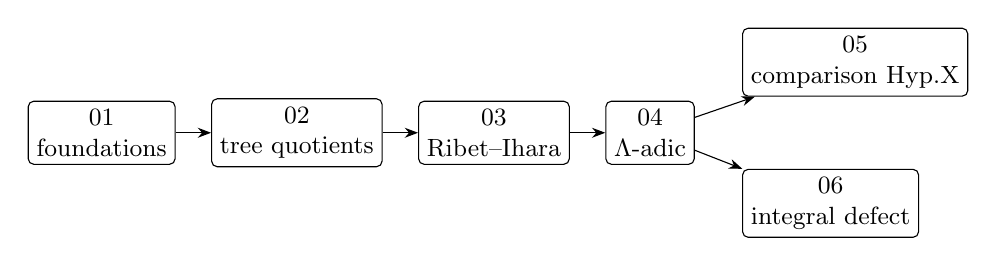
\begin{tikzpicture}[node distance=0.5cm and 0.45cm, >={Stealth},
  st/.style={draw,rounded corners=2pt,inner sep=3pt,font=\small,align=center}]
  \node[st] (s1) {01\\foundations};
  \node[st,right=of s1] (s2) {02\\tree quotients};
  \node[st,right=of s2] (s3) {03\\Ribet--Ihara};
  \node[st,right=of s3] (s4) {04\\$\Lambda$-adic};
  \node[st,above right=0.05cm and 0.6cm of s4] (s5) {05\\comparison $\HypX$};
  \node[st,below right=0.05cm and 0.6cm of s4] (s6) {06\\integral defect};
  \draw[->] (s1)--(s2); \draw[->] (s2)--(s3); \draw[->] (s3)--(s4); \draw[->] (s4)--(s5); \draw[->] (s4)--(s6);
\end{tikzpicture}
\caption{Dependency of the six stages: a chain of arrows from stage 01 (foundations) to stage 02 (tree quotients), stage 03
(Ribet sequence and Ihara lemma) and stage 04 ($\Lambda$-adic passage); from stage 04 two arrows branch to stage 05 (the comparison
hypothesis $\HypX$) and to stage 06 (the integral defect), which are independent of each other: stage 06 does not use $\HypX$.}
\label{fig:stages}
\end{figure}

\IfFileExists{stage01.tex}{% SPDX-License-Identifier: CC-BY-4.0
% Copyright (C) 2026 Fabian Januszewski, Abhijit (the Langlandscape team)
% Stage 01 section of the submission report (proof outlines condensed from mathematics/chapters/s01; statements verbatim).
% Note: the literature-folder pointers (lit macro) of the chapter text (also inside the verbatim boxes) were mechanically
% converted to \cite[loc]{KEY} with the keys of report.bib; cross-references were replaced by main.pdf numbers.
\subsection{Stage 01: quaternionic foundations}\label{ss:stage01}
Stage 01 fixes the definite side of the Jacquet--Langlands correspondence over $\Q$: the quaternion algebra $B=\Bd$,
its levels and class sets, the Eichler mass formula, Brandt modules and the Brandt pairing, the Hecke operators with
the fixed normalisation $\NUp$ of $U_p$, the dictionary to the conventions of the literature, and the cited targets
(classical, $p$-adic and $\Lambda$-adic JL). Every later stage uses these objects: the class sets $S_s=\XB{U_s}$ are the
vertex sets of the Brandt graphs of stage 02, the Brandt pairing and the norm map $\nu$ give the self-duality used in stages
03 and 06, and $\NUp$ is the normalisation in which the ordinary projector of stage 04 is compatible with the $p$-tower.
In main.pdf this is Sections 1--6, pp.~27--50.
\begingroup\sloppy

\subsubsection*{Key definitions}
\emph{Algebra and levels} (main.pdf, Def.~1.1 and Def.~1.2, p.~27). $D>1$ is squarefree with $\omega(D)$ odd; $B=\Bd$ is the
quaternion algebra over $\Q$ ramified exactly at $\infty$ and the primes $\ell\mid D$; $\cO\subset B$ is a maximal order,
$\iota_\ell:\cO_\ell\xrightarrow{\sim}M_2(\Z_\ell)$ is fixed for $\ell\nmid D$, and for $\ell\mid D$ $\Pi_\ell$ is a uniformiser
of the division algebra $B_\ell$ ($\Pi_\ell^2\in\ell\,\cO_\ell^\times$). For $N\ge1$, $(N,D)=1$: $\Uzero N$, $\Uone N\subseteq\hat\cO^\times$
are the products of the local groups $\{(\begin{smallmatrix}a&b\\c&d\end{smallmatrix})\in\GL_2(\Z_\ell):c\equiv0\}$, resp.\
$\{c\equiv0,\ d\equiv1\}$, modulo $\ell^{v_\ell(N)}$ (\emph{lower} row $\equiv(0,1)$, Buzzard's convention). Further
$U_s:=\Uone{Mp^s}$ with $(Mp,D)=1$, $S_s:=\XB{U_s}$, $\Delta_s:=(1+p\Zp)/(1+p^s\Zp)$, and $U_0(q)U:=U\cap\Uzero q$ for an auxiliary
prime $q\nmid D$ with $U_q=\cO_q^\times$.

\emph{Class sets} (main.pdf, Def.~1.5, p.~29). For compact open $U\subseteq\hat\cO^\times$: $\XB U=B^\times\backslash\Bhat^\times/U$,
$\Gamma_x=B^\times\cap xUx^{-1}$, $w_x=|\Gamma_x/(\Gamma_x\cap\{\pm1\})|$; so $|\Gamma_x|=\varepsilon\,w_x$ with
$\varepsilon=|\{\pm1\}\cap U|$ independent of $x$.

\emph{Coefficients} (main.pdf, eq.~(1), p.~32). $V_k=\Sym^{k-2}(\Zp^2)$ as homogeneous polynomials of degree $n=k-2$, with the
left action $(g\cdot P)(X,Y)=P((X,Y)g)$ of the monoid $\Sigma_p=M_2(\Zp)\cap\GL_2(\Qp)$; $\mathrm{ev}(P)=P(0,1)$ satisfies
$\mathrm{ev}(g\cdot P)\equiv d^n\mathrm{ev}(P)\pmod c$. \stproved{}

\emph{Brandt module} (main.pdf, Def.~3.1, p.~33). $\Brandt UV=\{f:\Bhat^\times\to V:\ f(\gamma xu)=u_p^{-1}f(x)\}\cong
\bigoplus_{[x]\in\XB U}V^{x_p^{-1}\Gamma_xx_p}$; for trivial $V=\Z$ one has $\Z^X$ (functions) and $\Z[X]$ (divisors),
dual under evaluation. \stknown{} \cite[(4.1)--(4.2), Prop.~4.5]{Gr99}; the isomorphism is \stproved.

\emph{Brandt pairing and norm map} (main.pdf, Def.~3.2, p.~33). $\langle[x],[y]\rangle=w_x\delta_{xy}$ on $\Z[X]$;
$\nu:\Z[X]\to\Z^X$, $[x]\mapsto w_x\mathbf 1_x$, so $\nu(a)=\langle a,\cdot\rangle$; $\nu$ is an isomorphism over $\Zp$ whenever
$p\nmid w_x$ for all $x$, in particular for $p\ge5$. \stproved{}, \stformal{} (\pathtt{Langlandscape.Brandt.normMap\_bijective},
$p$-adic version \pathtt{Langlandscape.Brandt.normMap\_bijective\_padic}). With $V_k$-coefficients the pairing is
$\langle f,h\rangle_k=\sum_xw_x^{-1}u_{x,p}^n\beta_n(f(x),h(x))$, $\beta_n(X^{n-i}Y^i,X^jY^{n-j})=\delta_{ij}(-1)^i\binom ni^{-1}$;
it is perfect over $\Zp$ if $p\nmid|\Gamma_x|$ and $p>k-2$ (exact range: $n+1=cp^a$, $1\le c\le p-1$)
(main.pdf, Def.~5.1, p.~42). \stproved{}

\emph{Hecke operators} (main.pdf, Def.~4.1, p.~35). For $g\in\Bhat^\times$ with $g_p\in\Sigma_p$ and $UgU=\coprod_ig_iU$:
$(T_gf)(x)=\sum_ig_{i,p}\cdot f(xg_i)$, and on $\Z[X]$ the transpose $T_g[x]=\sum_i[xg_i]$. Named operators:
$T_\ell=T_{\varpi_\ell}$, $\varpi_\ell=\iota_\ell^{-1}\mathrm{diag}(\ell,1)$, and $S_\ell=T_{z_\ell}$ ($z_\ell$ the central idele $\ell$
at $\ell$) for $\ell\nmid DMpq$; $U_\ell=T_{\varpi_\ell}$ for $\ell\mid M$; the diamond $\langle d\rangle=T_{\delta_d}$, right translation
by $\delta_d=\mathrm{diag}(1,d)$ at the primes dividing $Mp$; $\Pi_\ell f=f(\cdot\,\Pi_\ell)$ for $\ell\mid D$; and $U_p=\NUp$ below.
Well-definedness \stproved; \stformal{} for trivial coefficients (\pathtt{Langlandscape.Brandt.heckeT}, \texttt{\dots Tl},
\texttt{\dots Sl}, \texttt{\dots Ul}, \texttt{\dots diamond}, \texttt{\dots PiEll}, \texttt{\dots Up}).

\begin{quoted}{Definition}{4.2}{36}{def:s01-NUp}{$N_{U_p}$: the normalisation of $U_p$ fixed for the whole plan}{chapters/s01/4-hecke.tex}\label{rpt:def:s01-NUp}
Let $s\ge1$ and $U=U^{(p)}U_p$ with $U_p\in\{K_s,K^0_s\}$. Put $\varpi_j:=\iota_p^{-1}\left(\begin{smallmatrix}p&j\\0&1\end{smallmatrix}\right)$,
$0\le j\le p-1$ (as elements of $\Bhat^\times$ supported at $p$). Then $U\varpi_pU=\coprod_{j=0}^{p-1}\varpi_jU$
(Lemma~4.3(a)) and
\[(U_pf)(x):=\sum_{j=0}^{p-1}\varpi_j\cdot f(x\varpi_j)\ \ \text{on }\Brandt{U}{V},\qquad U_p[x]:=\sum_{j=0}^{p-1}[x\varpi_j]\ \ \text{on }\Z[\XB{U}],\]
with $\varpi_j$ acting on $V_k$ by (1). This is $N_{U_p}$. Its features:
\begin{itemize}
\item it is \emph{integral}: $\varpi_j\in\Sigma_p$ acts on $V_k$ by $P\mapsto P(pX,\,jX+Y)$, which preserves $V_k$;
\item it needs \emph{no} normalising power of $p$: on the line $\mathrm{ev}:V_k\to\Zp$, $P\mapsto P(0,1)$, one has
  $\mathrm{ev}(\varpi_jP)=P((0,1)\varpi_j)=P(0,1)$, i.e.\ each $\varpi_j$ acts by its $(2,2)$ entry $1$;
\item $\Brandt{U}{V_k}$ is finite free over $\Zp$, so the ordinary projector $e=\lim_nU_p^{n!}$ exists.
\end{itemize}
\stproved{} (integrality, the $\mathrm{ev}$-computation, and the existence of $e$ for any endomorphism of a finite free $\Zp$-module).
\emph{Correction:} the stage tex adds that $e$ ``is non-trivial in every weight''. At a fixed level this is false: for
$D=2$, $M=1$, $p=5$, $s=1$, $k=2$ (trivial $V=\Z_5$) one has $|S_1|=\frac{1}{24}\cdot1\cdot6\cdot4=1$ (Thm.~2.1(d)), so
$\Brandt{U}{\Z_5}=\Z_5$ consists of the constants, $U_p=5$ on it, and $e=0$ \stproved. More generally, with trivial coefficients
$U_p\mathbf 1=p\,\mathbf 1$, so the constant (Eisenstein) line is never ordinary. What is true: $e$ exists and splits
$\Brandt{U}{V_k}=e\Brandt{U}{V_k}\oplus(1-e)\Brandt{U}{V_k}$ as $\Zp[U_p]$-modules (Fitting decomposition, \stproved); the
rank of the ordinary part is controlled in the tower (independence of $k\ge2$ and of $s\ge1$ after fixing the nebentypus at $p$,
Hida's control theorem: \stexp{} here and owned by stage 04); whether it is nonzero for given $(D,M,p)$ is a computation.
\lean{Langlandscape.Local.varpi}, \lean{Langlandscape.Local.varpiDiag}, \lean{Langlandscape.Brandt.Up},
\lean{Langlandscape.Brandt.Up\_apply} \stformal{} (trivial coefficients).
\end{quoted}
Here $K_s=U_1(p^s)_p$, $K^0_s=U_0(p^s)_p$, $\varpi=\mathrm{diag}(p,1)$, $\eta=\mathrm{diag}(1,p)$ (main.pdf, p.~35).
The ``other'' operator $U'_p:=[U\eta_pU]$, $\eta_p=\iota_p^{-1}\mathrm{diag}(1,p)$, is the literal formula of the project's original
planning document (the ``seed''); Lemma~4.3 below shows why it is not used.

\emph{Hecke algebras} (main.pdf, Def.~4.6, p.~41). $\T_B(U;V)\subseteq\End\Brandt UV$ is the $\Zp$-algebra generated by
$T_\ell,S_\ell^{\pm1}$ ($\ell\nmid DMpq$), $U_\ell$ ($\ell\mid M$), $\langle d\rangle$, $U_p$ ($s\ge1$) and $\Pi_\ell$ ($\ell\mid D$); it is
commutative (main.pdf, Prop.~4.4(c)) and finite free over $\Zp$. Under $\nu$ (trivial coefficients, $p\nmid w_x$), $T\mapsto\nu T\nu^{-1}$
maps $\T_B$ onto the algebra generated by the $T_{g^{-1}}$: $T_\ell\mapsto S_\ell^{-1}T_\ell$, $\langle d\rangle\mapsto\langle d\rangle^{-1}$,
$\Pi_\ell\mapsto\Pi_\ell^{-1}$, $U_p\mapsto\langle p\rangle_MU'_p$. So $\T_B$ is \emph{not} stable under adjunction (because of $U_p$), and
$\nu$ identifies $\Zp[X]$ and $\Zp^X$ as $\T_B$-modules only after the twist $T\mapsto T^\dagger$. \stproved{}

\subsubsection*{Main results and proof outlines}
Statements are quoted verbatim from main.pdf; each is followed by an outline of the proof given there.

\begin{quoted}{Proposition}{1.6}{29}{prop:s01-finite}{finiteness}{chapters/s01/1-classsets.tex}\label{rpt:prop:s01-finite}
$\XB{U}$ is finite and every $\Gamma_x$ is finite; $\Gamma_x\le\Gamma_x(\hat\cO^\times)=\cO_x^\times$ with $\cO_x=B\cap x\hat\cO x^{-1}$,
and $|\cO_x^\times|\in\{2,4,6,12,24\}$ ($\cO_x$ is \emph{maximal}; the value $8$ of Voight's list is the Lipschitz order,
which is non-maximal and occurs only for $D=2$). Consequently $|\Gamma_x|$ divides $24$ for every $U\subseteq\hat\cO^\times$.
\stknown{} \stformal{} (\lean{Langlandscape.Quat.XB\_finite}, \lean{Langlandscape.Quat.card\_Gam\_dvd\_24}) \cite[Thm.~17.1.1, p.~278 (finiteness); Thm.~11.5.14, p.~176
(unit groups of definite orders over $\Q$)]{Vo}; \cite[Prop.~4.3, p.~69]{Gr99}.
\emph{Existing material} (\stformal): \Tpath{P2/ClassSet.lean} \texttt{classSet}, \pathtt{classSet\_finite},
\pathtt{classSet\_finite\_of\_open} (any open $U\le\hat\cO^\times$), \texttt{classStabilizer}, \pathtt{stabilizer\_units}
(c): $|\Gamma_x|\in\{2,4,6,8,12,24\}$ at level $\hat\cO^\times$ (a superset: $8$ does not occur there); \Tpath{P2/Compact.lean} \pathtt{quotient\_compact}.
\end{quoted}
\begin{outline}
(1) $[\hat\cO^\times:U]<\infty$, so $\XB U\to\XB{\hat\cO^\times}$ has finite fibres (images of $x\hat\cO^\times/U$); the base is the right
class set of $\cO$, finite by \cite[Thm.~17.1.1]{Vo} \stcited.
(2) $\cO_x=B\cap x\hat\cO x^{-1}$ is an order with $\cO_x^\times=B^\times\cap x\hat\cO^\times x^{-1}\supseteq\Gamma_x$; it is maximal because
its completions $x_\ell\cO_\ell x_\ell^{-1}$ are \cite[Thm.~9.4.9]{Vo} \stcited.
(3) By \cite[Thm.~11.5.14]{Vo} \stcited, $|\cO_x^\times|\in\{2,4,6,8,12,24\}$, and $8$ occurs only for the Lipschitz order, which
has index $2$ in the Hurwitz order and is not maximal. Lagrange gives $|\Gamma_x|\mid24$. \stproved{} from these inputs;
\stformal{} as \pathtt{Langlandscape.Quat.XB\_finite}, \pathtt{Langlandscape.Quat.card\_Gam\_dvd\_24}.
\end{outline}

\begin{quoted}{Lemma}{1.7}{29}{lem:s01-stab}{stab; seed Lemma 5.2, reproved}{chapters/s01/1-classsets.tex}\label{rpt:lem:s01-stab}
Let $p\ge5$ (used only in (b) and (c)).
\begin{enumerate}[label=(\alph*)]
\item $\Nrd(\Gamma_x)=1$ for every $U$ with $\Nrd U=\Zhat^\times$ and every $x$.
\item If $p\nmid D$ and $U\subseteq\Uone{p}$ (at $p$), then every $\Gamma_x$ is trivial. If moreover $U=U^{(p)}\times U_{1}(p^s)_p$ with $s\ge1$,
  then $\Delta_s$, acting by $[x]\mapsto[x\,\iota_p^{-1}\mathrm{diag}(1,d)]$, acts freely on $\XB{U}$.
\item For every $U\subseteq\hat\cO^\times$, $p\nmid|\Gamma_x|$; in particular $p\nmid w_x$.
\end{enumerate}
\stproved. \stformal{} (\lean{Langlandscape.Quat.nrd\_eq\_one\_of\_mem\_Gam}, \lean{Langlandscape.Quat.card\_Gam\_dvd\_24},
\lean{Langlandscape.Quat.not\_dvd\_card\_Gam} for (a), (c); \lean{Langlandscape.Quat.Gam\_eq\_bot\_of\_le\_U1} for (b); (b$'$) for the tower only,
\lean{Langlandscape.Quat.diamondAct\_free}.)
\end{quoted}
\begin{outline}
(a) For $\gamma=xux^{-1}\in\Gamma_x$, $\Nrd\gamma=\Nrd u\in\Zhat^\times$ and $\Nrd\gamma\in\Nrd(B^\times)=\Q_{>0}$ ($B$ definite), and
$\Q_{>0}\cap\Zhat^\times=\{1\}$. \stproved{} (that $\Nrd U=\Zhat^\times$ at all standard levels is main.pdf, Lemma~1.3, \stproved{},
with the local structure at $\ell\mid D$ cited from \cite[Thm.~13.3.11]{Vo}.)
(b) \emph{Triviality.} $\gamma\in\Gamma_x$ has finite order and $\Nrd\gamma=1$, so its reduced characteristic polynomial is $X^2-tX+1$ with
$t\in\Z$, $|t|\le2$; $t=\pm2$ forces $(\gamma\mp1)^2=0$, hence $\gamma=\pm1$ since $B$ is a division algebra. If $\gamma\ne1$ then
$t\in\{-2,-1,0,1\}$. The reduction mod $p$ of $\iota_p(x_p^{-1}\gamma x_p)\in U_{1,p}$ is upper triangular with $(2,2)$ entry $1$, so $1$ is a root of
$X^2-\bar tX+1$, i.e.\ $p\mid2-t\in\{4,3,2,1\}$, impossible for $p\ge5$.
\emph{Freeness of $\Delta_s$.} $\delta_d$ normalises $U$, so $[x]\mapsto[x\delta_d]$ is well defined and factors through $\Delta_s$. If
$x\delta_d=\gamma xu$ with $d\in1+p\Zp$, then $\gamma\in B^\times\cap xU'x^{-1}$ for $U'=U\langle\delta_d\rangle$, still contained in $\Uone p$ at $p$;
by the first part $\gamma=1$, so $\delta_d\in U$ and $d\equiv1\bmod p^s$. (Only $\Delta_s$, not the full diamond group, acts freely.)
An alternative route avoiding Cayley--Hamilton mod $p$ (a case list of the $(2,2)$ entry of $u^2$) is the one formalized
(main.pdf, Rem.~1.8). \stproved{}, \stformal{} (\pathtt{Langlandscape.Quat.Gam\_eq\_bot\_of\_le\_U1}, \pathtt{Langlandscape.Quat.diamondAct\_free}).
(c) $|\Gamma_x|$ divides $24$ by Prop.~1.6, and $w_x\mid|\Gamma_x|$. \stproved.
\end{outline}

\begin{quoted}{Theorem}{2.1}{31}{thm:s01-mass}{Eichler mass formula; \texttt{if:s01-mass}}{chapters/s01/2-mass.tex}\label{rpt:thm:s01-mass}
\begin{enumerate}[label=(\alph*)]
\item $\displaystyle\sum_{[x]\in\XB{\hat\cO^\times}}\frac1{|\Gamma_x|}=\frac{1}{24}\prod_{\ell\mid D}(\ell-1)$
  (full-unit convention), equivalently $\sum 1/w_x=\varphi(D)/12$.
\item (level change) For open $U'\le U\le\hat\cO^\times$: $\sum_{X_B(U')}1/|\Gamma_{x'}(U')|=[U:U']\sum_{X_B(U)}1/|\Gamma_x(U)|$.
  With $w$ in place of $|\Gamma|$ the same holds iff $-1\in U'$ or $-1\notin U$; if $-1\in U\setminus U'$ then
  $2\sum_{X_B(U')}1/w_{x'}=[U:U']\sum_{X_B(U)}1/w_x$ (\lean{Langlandscape.Quat.massW\_level\_change\_two}).
\item $[\hat\cO^\times:\Uzero{N}]=\psi(N)=N\prod_{\ell\mid N}(1+\ell^{-1})$ and $[\hat\cO^\times:\Uone{N}]=\psi(N)\varphi(N)=N^2\prod_{\ell\mid N}(1-\ell^{-2})$.
\item Hence $\sum_{\XB{\Uzero{N}}}1/w_x=\varphi(D)\psi(N)/12$, and for $p\ge5$, $p\nmid D$, $s\ge1$, $(M,pD)=1$:
\[|S_s|=|\XB{\Uone{Mp^s}}|=\frac{\varphi(D)}{24}\,\psi(Mp^s)\,\varphi(Mp^s).\]
\end{enumerate}
Status: (a) \stcited{} \cite[Thm.~25.1.1, p.~415 (with $w_J=\#\cO_L(J)^\times/\{\pm1\}$,
hence $1/12$)]{Vo}; \cite[\S4 ``Klassenzahl und Maß'', p.~136ff.]{Eic55};
in Lean it is the registered hypothesis \pathtt{Hyp.EichlerMass} (\Tpath{Hyp/EichlerMass.lean}, $1/24$, full units), proved
for $D=2,11$ in tests. (b) \stformal{} \Tpath{P2/Mass.lean} \pathtt{mass\_orbit\_count}; the $w$-variant \stformal{} \pathtt{Quat.massW\_level\_change},
\pathtt{Quat.massW\_level\_change\_two} (orbit counting). (c) first half \stformal{} \pathtt{gl2\_borel\_index}, \pathtt{mass\_level\_change}; second half
\stproved{} below (count $|\GL_2(\Z/N)|/(N\varphi(N))$). (d) first half \stpmc{} from (a)--(c) (proof below; cf.\ \cite[Thm.~25.3.18,
p.~423]{Vo}), \stpmc{} in Lean as \pathtt{eichlerOrder\_mass} (under \pathtt{Hyp.EichlerMass}); second half \stpmc{} from (a)--(c)
and Lemma~1.7(b) (all $\Gamma_x=1$), and \stformal{} under \pathtt{Hyp.EichlerMass} as \pathtt{Quat.card\_XB\_Utower}.
\end{quoted}
\begin{outline}
(a) Not proved here: \stcited{} \cite[Thm.~25.1.1]{Vo}, \cite[\S4]{Eic55}. In Lean the registered hypothesis \pathtt{Hyp.EichlerMass}
(open, cited; its closed instances live only in the import's test library and are not reachable from our build).
(b) Let $\pi:\XB{U'}\to\XB U$ and $\Gamma=\Gamma_x(U)$. Then $uU'\mapsto[xu]$ induces a bijection $\Gamma\backslash(U/U')\xrightarrow\sim\pi^{-1}([x])$,
and the stabiliser of $uU'$ in $\Gamma$ is $\Gamma_{xu}(U')$. Orbit--stabiliser gives
$\sum_{[x']\in\pi^{-1}[x]}1/|\Gamma_{x'}(U')|=[U:U']/|\Gamma_x(U)|$; sum over $[x]$. For $w$: $w_x=|\Gamma_x|/\varepsilon(U)$ with
$\varepsilon(U)=2$ iff $-1\in U$, so the $w$-sums differ by the ratio $\varepsilon(U')/\varepsilon(U)\in\{1,\tfrac12\}$; the ratio is $\tfrac12$
exactly when $-1\in U\setminus U'$ (the ``factor~2''). \stproved, \stformal.
(c) Local at $\ell^k\Vert N$: $\GL_2(\Z_\ell)$ acts transitively on $\mathbb P^1(\Z/\ell^k)$ (size $\ell^k+\ell^{k-1}$) with stabiliser
$U_{0,\ell}$; and $g\mapsto d\bmod\ell^k$ is a surjective homomorphism $U_{0,\ell}\to(\Z/\ell^k)^\times$ with kernel $U_{1,\ell}$ (the $(2,2)$ entry of a
product is $cb'+dd'\equiv dd'$). \stproved{} (first half also \stformal).
(d) $-1\in\Uzero N$, so (b), (c), (a) give the first formula. For $U=\Uone{Mp^s}$ ($p\ge5$, $s\ge1$) all $\Gamma_x$ are trivial by
Lemma~1.7(b), so $|\XB U|=\sum1/|\Gamma_x|=[\hat\cO^\times:U]\,\varphi(D)/24$. The only cited input is (a); hence \stpmc.
\emph{Checks} (main.pdf, Ex.~2.2, \stpmc): $D=2$ has class number $1$ and $|\cO^\times|=24$; $D=3$, $p=5$, $M=1$ gives $|S_s|=2\cdot25^{s-1}$,
and $|S_s|=2,50,1250$ for $s=1,2,3$ is \stcomp{} (\res{s01/levels.json}); $D=11$: two classes with $|\Gamma_x|=4,6$ (using the cited
class number $h=2$, \cite[Thm.~30.1.5]{Vo}).
\end{outline}

\begin{quoted}{Proposition}{3.3}{33}{prop:s01-adjoint}{adjoints; equivariance of $\nu$}{chapters/s01/3-brandt.tex}\label{rpt:prop:s01-adjoint}
Let $T_g=[UgU]$ act on $\Z^X$ by $f\mapsto\sum_if(xg_i)$ and on $\Z[X]$ by its transpose $[x]\mapsto\sum_i[xg_i]$
($UgU=\coprod_ig_iU$, $g$ supported away from $p$ or trivial coefficients). Then
\begin{enumerate}[label=(\alph*)]
\item the $\langle,\rangle$-adjoint of $T_g$ on $\Z[X]$ is $T_{g^{-1}}$;
\item $\nu\circ T_g=T_{g^{-1}}\circ\nu$. In particular $\nu$ intertwines $T_\ell$ with $S_\ell^{-1}T_\ell$, $\langle d\rangle$ with
  $\langle d\rangle^{-1}$, $\Pi_\ell$ with $\Pi_\ell^{-1}$, and $U_p$ with $U_p^{*}$ (Lemma~4.3(d)). At level
  $\Uzero{M}$ with trivial coefficients, $S_\ell=1$ and $T_\ell$ ($\ell\nmid DM$) is self-adjoint and $\nu$-equivariant.
\item for finite $\pi:X'=X_B(U')\to X=X_B(U)$ ($U'\le U$), \emph{assuming $-1\in U'$ or $-1\notin U$}: $\nu\circ\pi_*=\mathrm{tr}\circ\nu'$, where
  $\mathrm{tr}f(x)=\sum_{u\in U/U'}f(xu)$. Dually, $\nu'\circ\pi^!=\pi^*\circ\nu$ for the transfer
  $\pi^![x]:=\sum_{u\in U/U'}[xu]'$ (the transpose of $\mathrm{tr}$) under the same assumption, whereas the multiplicity-free fibre sum
  $\pi^\sharp[x]=\sum_{x'\in\pi^{-1}[x]}[x']$ does \emph{not} satisfy $\nu'\circ\pi^\sharp=\pi^*\circ\nu$ in general.
  Without the assumption, $\mathrm{tr}\circ\nu'=2\,\nu\circ\pi_*$ and $\nu'\circ\pi^!=2\,\pi^*\circ\nu$.
\end{enumerate}
Status: (a) \stcited{} \cite[Prop.~6.9, p.~73 (adjoint of $T(g)$ is $\mu_A(g)T(g^{-1})$;
$\mu=1$ for trivial $V$)]{Gr99}, and \stproved{} below for trivial coefficients (any $g\in\Bhat^\times$); \stformal{} for $T_n$, $(n,DM)=1$, level $\hat\cO(M)^\times$, all $k$:
\Tpath{Brandt/Pairing.lean} \pathtt{hecke\_self\_adjoint}, \Tpath{Brandt/Brandt.lean} \pathtt{brandt\_weighted\_symmetry}
($|\Gamma_{x_{c'}}|B(n)_{cc'}=|\Gamma_{x_c}|B(n)_{c'c}$); general $g$: \lean{Langlandscape.Brandt.brandtPairing\_heckeTHom} \stformal{}.
(b) \stproved{} below; \lean{Langlandscape.Brandt.normMap\_heckeT} \stformal{}; the ``in particular'' clauses:
\lean{Langlandscape.Brandt.Tl\_adjoint}, \lean{Langlandscape.Brandt.diamond\_adjoint}, \lean{Langlandscape.Brandt.PiEll\_adjoint},
\lean{Langlandscape.Brandt.Tl\_selfAdjoint\_U0} \stformal{} (the $U_p$ clause is Lemma~4.3(d)).
(c) \stproved{} below, with the factor-2 case (F3); \lean{Langlandscape.Brandt.normMap\_pushforward},
\lean{Langlandscape.Brandt.normMap\_pushforward\_two} \stformal{}.
\end{quoted}
\begin{outline}
(a) For $x,y$ let $N_g(x,y)=\#\{i:[xg_i]=[y]\}$, so $\langle T_g[x],[y]\rangle=w_yN_g(x,y)$. The set $P=\{\gamma\in B^\times:\gamma y\in xUgU\}$ maps onto
$\{i:[xg_i]=[y]\}$ with fibres the cosets $\gamma\Gamma_y$, so $|P|=N_g(x,y)|\Gamma_y|$. Inversion maps $P$ bijectively to the analogous set for
$(y,x,g^{-1})$, so $N_g(x,y)|\Gamma_y|=N_{g^{-1}}(y,x)|\Gamma_x|$; dividing by $\varepsilon$ gives
$\langle T_g[x],[y]\rangle=\langle[x],T_{g^{-1}}[y]\rangle$. (The weights $|\Gamma|$ are what make the count symmetric.) \stproved{} for trivial
coefficients; the general statement is Gross's Prop.~6.9 \cite[Prop.~6.9]{Gr99} \stcited.
(b) Formal from (a) and $\nu(a)(y)=\langle a,[y]\rangle$. For the named operators: $z_\ell$ is central, $\delta_d$ and $\Pi_\ell$ normalise $U$
(single cosets), and $\varpi_\ell^{-1}=z_\ell^{-1}\iota_\ell^{-1}\mathrm{diag}(1,\ell)$ with $[U\mathrm{diag}(1,\ell)U]=[U\varpi_\ell U]$ for $\ell\nmid$ level,
whence $T_\ell^*=S_\ell^{-1}T_\ell$. \stproved.
(c) One computes $\mathrm{tr}\,\mathbf 1_{[x]'}=[\Gamma_x:\Gamma'_x]\mathbf 1_{[x]}$ (the $u\in U/U'$ with $xu\in B^\times xU'$ form the image of $\Gamma_x$, with
fibres $\Gamma'_x$-cosets), hence $\mathrm{tr}\,\nu'[x]'=(\varepsilon/\varepsilon')\,\nu\pi_*[x]'$; the transfer is the same computation. For $\pi^\sharp$
the coefficient $w'_z$ differs from $w_x$ as soon as $[\Gamma_x:\Gamma'_z]\ne\varepsilon/\varepsilon'$ (example: $D=2$, $U'=\Uzero3$, $w'_z=3\ne12=w_x$). \stproved.
\emph{Consequence} (main.pdf, Rem.~3.4): $\nu$ is an isomorphism of Hecke modules only after replacing each operator by its adjoint, and
$\pi_*$ on divisors corresponds to the trace on functions, not to pullback.
\end{outline}

\begin{quoted}{Lemma}{4.3}{37}{lem:s01-Up}{properties of $N_{U_p}$}{chapters/s01/4-hecke.tex}\label{rpt:lem:s01-Up}
Let $s\ge1$, $U_{(s)}:=U^{(p)}K_s$, $\pi=\pi_{s+1,s}:\XB{U_{(s+1)}}\to\XB{U_{(s)}}$, $\pi^*:\Brandt{U_{(s)}}{V}\hookrightarrow\Brandt{U_{(s+1)}}{V}$
the inclusion, and $\mathrm{tr}=\mathrm{tr}_{s+1,s}:\Brandt{U_{(s+1)}}{V}\to\Brandt{U_{(s)}}{V}$,
$\mathrm{tr}f(x)=\sum_{u\in U_{(s)}/U_{(s+1)}}u_p\cdot f(xu)$.
\begin{enumerate}[label=(\alph*)]
\item $K\varpi K=\coprod_{j=0}^{p-1}\varpi_jK$ for $K\in\{K_s,K^0_s\}$; so the coset representatives $\varpi_j$ of $U_{(s)}\varpi_pU_{(s)}$ do
  not depend on $s\ge1$ (nor on $U_1$ versus $U_0$). For $s=0$ this fails: $K_0\varpi K_0$ has $p+1$ cosets.
\item $U_p\circ\pi^*=\pi^*\circ U_p$ on $\Brandt{U_{(s)}}{V}\subseteq\Brandt{U_{(s+1)}}{V}$, and dually $\pi_*\circ U_p=U_p\circ\pi_*$
  on $\Zp[S_{s+1}]\to\Zp[S_s]$. \textbf{This is the property demanded by the seed; $N_{U_p}$ is the normalisation with it.}
\item $[K_s:K_{s+1}]=p^2$ (for $s\ge1$; $[K_0:K_1]=p^2-1$). The other operator $U_p':=[U\,\eta_p\,U]$, $\eta_p=\iota_p^{-1}\mathrm{diag}(1,p)$
  (the seed's literal formula), has at level $U_{(s)}$ the representatives
  $\eta^{(s)}_j:=\iota_p^{-1}\left(\begin{smallmatrix}1&0\\p^sj&p\end{smallmatrix}\right)$, $0\le j\le p-1$, which depend on $s$; all $p$ of the
  level-$(s+1)$ representatives lie in the single coset $\eta_pU_{(s)}$, so $U'_p\pi^*f=p\cdot\eta_p\cdot R(\eta_p)f$ in
  $\Brandt{U_{(s+1)}}{V}$. For $\Zp$-torsion free $V$, $U'_p\pi^*=\pi^*U'_p$ on $\Brandt{U_{(s)}}{V}$ forces
  $U'_p\equiv0\pmod p$ there; so the two \emph{fail} to commute as soon as $U'_p\not\equiv0\pmod p$ on $\Brandt{U_{(s)}}{V}$, e.g.\
  (trivial $V$, $p\ge5$, $U^{(p)}=\Uone M$) whenever $e\Zp[S_s]\ne0$. They \emph{can} commute: for $D=2$, $M=1$, $p=5$, $s=1$, trivial $V$, both sides
  equal multiplication by $p$ on the constants $\Brandt{U_{(1)}}{\Z_5}=\Z_5$. Instead $U'_p$
  commutes with the trace, $\mathrm{tr}\circ U'_p=U'_p\circ\mathrm{tr}$, because $U_{(s)}\eta_pU_{(s)}=U_{(s)}\eta_pU_{(s+1)}$.
\item (trivial coefficients, $U^{(p)}=\Uone{M}$, i.e.\ $U_{(s)}=\Uone{Mp^s}$) The $\langle,\rangle$-adjoint of $U_p$ on $\Z[S_s]$ is
  $U_p^*=\langle p\rangle_M\,U_p'$, where $\langle p\rangle_M:=\langle d\rangle$ for the $d\in(\Z/Mp^s)^\times$ with $d\equiv p\bmod M$,
  $d\equiv1\bmod p^s$ (the diamond at the primes dividing $M$); so under $\nu$ the homological $U_p$ on $\Zp[S_s]$ becomes
  $\langle p\rangle_MU'_p$ on $\Zp^{S_s}$: $\nu\circ U_p=\langle p\rangle_MU'_p\circ\nu$ (consistent with (b), (c) and
  Prop.~3.3(c)).
\item For $s\ge1$ and $\ell\nmid Mp$, $U_p$ commutes with $T_\ell,S_\ell,\langle d\rangle,\Pi_\ell$, and with right translation by
  $B_q^\times$ ($q\ne p$), in the form of Prop.~4.4(c).
\end{enumerate}
\emph{Correction:} the stage tex writes $U'_p\pi^*f=p\cdot\pi^*R(\mathrm{diag}(1,p))f\ne\pi^*U'_pf$ (trivial $V$). The factor
$\pi^*$ is wrong, since $R(\eta_p)f$ is in general not in $\pi^*\Brandt{U_{(s)}}{V}$, and for non-trivial $V$ the action $\eta_p\cdot$ on $V$ must be added;
the inequality is not unconditional (see the example above). The corrected statement is (c) as given here.

Status: (a)--(e) \stproved{} below, except the \emph{existence} of a level where $U'_p\pi^*\ne\pi^*U'_p$: the sufficient
criterion of (c) is proved, and an explicit failure is \stcomp{} (S01-C5, \pathtt{code/results/s01/up.json}: $B_3$, $p=5$, $s=1,2$; $U_5$ on $S_1$ has eigenvalues $5,1$). (d) is derived here from the orbit-counting form of Prop.~3.3(a), which
is re-proved in the proof of (d) for trivial coefficients.
(a): \lean{Langlandscape.Local.K1\_mul\_varpi\_mul\_K1}, \lean{Langlandscape.Local.varpi\_inv\_mul\_not\_mem},
\lean{Langlandscape.Local.reps\_indep}; (b): \lean{Langlandscape.Brandt.Up\_comm\_push}, \lean{Langlandscape.Brandt.Up\_comm\_pull};
(c), coset half: \lean{Langlandscape.Local.diag1p\_reps}, \lean{Langlandscape.Local.relIndex\_K1\_succ}; (e):
\lean{Langlandscape.Brandt.Up\_comm\_Tl}; all \stformal{}. The trace half of (c) and (d) have no Lean counterpart in stage 01.
\end{quoted}
\begin{outline}
Throughout, $k=(\begin{smallmatrix}a&b\\c&d\end{smallmatrix})\in K$ with $s\ge1$ has $c\in p\Zp$, hence $a,d\in\Zp^\times$.
\begin{enumerate}[label=(\arabic*)]
\item (a) The fibres of $K\to K\varpi K/K$ are the cosets of $K'=K\cap\varpi K\varpi^{-1}=\{k\in K:b\in p\Zp\}$. As $d$ is a unit there is exactly
one $j\in\{0,\dots,p-1\}$ with $b-jd\in p\Zp$, so $K=\coprod_jn(j)K'$ and $K\varpi K=\coprod_jn(j)\varpi K$, $n(j)\varpi=\varpi_j$; disjointness since
$\varpi_j^{-1}\varpi_{j'}=n((j'-j)/p)\notin\GL_2(\Zp)$. For $s=0$, $d$ need not be a unit and $\eta$ is an extra $(p+1)$-st representative.
\stproved, \stformal.
\item (b) By (a) the same $\varpi_j$ represent the double coset at levels $s$ and $s+1$, so $U_p\pi^*$ and $\pi^*U_p$ are literally the same
formula; the divisor statement is the transpose. \stproved, \stformal.
\item (c) \emph{Index}: $K_s$ is the stabiliser of the bottom row $(0,1)\bmod p^s$, and $K_s/K_{s+1}$ is the set of bottom rows
$(c,d)\bmod p^{s+1}$ with $(c,d)\equiv(0,1)\bmod p^s$, of size $p^2$ (consistent with $|S_{s+1}|=p^2|S_s|$). \emph{Representatives of $U'_p$}:
$K_s\cap\eta K_s\eta^{-1}=\{c\in p^{s+1}\Zp\}$, giving $\eta_j^{(s)}$, which depend on $s$; all level-$(s+1)$ representatives lie in $\eta K_s$,
whence $U'_p\pi^*f=p\,\eta_p R(\eta_p)f$. Since $\pi^*\Brandt{U_{(s)}}V$ is saturated, $U'_p\pi^*=\pi^*U'_p$ would force $U'_p\equiv0\pmod p$, which
by (d) and perfectness of the pairing ($p\ge5$) is equivalent to $U_p\equiv0\pmod p$ on $\Zp[S_s]$ and would force $e\Zp[S_s]=0$.
\emph{Trace}: $K_s=LK_{s+1}$ with $L=K_s\cap\eta^{-1}K_s\eta$, so $U_{(s)}\eta_pU_{(s)}=U_{(s)}\eta_pU_{(s+1)}$; both $\{\eta_iu\}$ and $\{u\eta'_{i'}\}$ are
representative systems of the same $p^3$-element set $U_{(s)}\eta_pU_{(s)}/U_{(s+1)}$, which gives $U'_p\,\mathrm{tr}=\mathrm{tr}\,U'_p$. \stproved;
the explicit non-commutation is \stcomp{} (\res{s01/up.json}).
\item (d) Step~1: the orbit count of Prop.~3.3(a) gives $U_p^*=T_{\varpi_p^{-1}}$. Step~2: $\varpi_p^{-1}=z_p^{-1}\eta_p$, $z_p$ central. Step~3: the
global $p\in\Q^\times$ is central, so $[yz_p^{-1}h]=[yth]$ with $t$ the scalar idele $p$ away from $p$ and $1$ at $p$; $t=\delta_d$ with $d\equiv p\bmod M$,
$d\equiv1\bmod p^s$, i.e.\ $R(t)=\langle p\rangle_M$. Hence $U_p^*=\langle p\rangle_MU'_p$. Step~4: apply Prop.~3.3(b). \stproved{} (trivial
coefficients; extended to $V_k$ in main.pdf, Lemma~5.3(d), via Gross's factor $\mu_A(g)=r_g^n$, \stproved{} with (d) also \stcited{}
from \cite[Prop.~6.9]{Gr99}).
\item (e) Operators supported at $\ell\ne p$ have representatives commuting with the $\varpi_j$; the diagonal $\delta_d$ normalises $U$ and
commutes with $\varpi_p$. \stproved, \stformal{} (\pathtt{Langlandscape.Brandt.Up\_comm\_Tl}).
\end{enumerate}
\end{outline}

\noindent\emph{Relations and the diamond convention} (main.pdf, Prop.~4.4, p.~39, and Rem.~4.5, p.~40). On
$\Brandt{\Uone{Mp^s}}{V_k}$, $S_\ell=\ell^{k-2}\langle\ell\rangle^{-1}$ ($\ell\nmid DMp$) and $\Pi_\ell^2=S_\ell$ ($\ell\mid D$), all operators
commute, those away from $q$ commute with right translation by $B_q^\times$, and $T_\ell T_{\ell^r}=T_{\ell^{r+1}}+\ell S_\ell T_{\ell^{r-1}}$.
Proof of the first formula: $f(xz_\ell)=f(\ell^{-1}xz_\ell)$ and $\ell^{-1}z_\ell$ is a scalar idele in $\Uzero{Mp^s}$ with lower right entries
$\ell^{-1}$, i.e.\ $\delta_{\ell^{-1}}$ times an element of $\Uone{Mp^s}$ whose $p$-component $\ell^{-1}I$ acts by $\ell^{-n}$. \stproved{}
(the recursion is also \stknown, \cite[Prop.~41.3.1, Prop.~41.3.6]{Vo}). Since classically $S_\ell=\ell^{k-2}\langle\ell\rangle$, \emph{the
adelic $\langle d\rangle$ corresponds to the classical $\langle d\rangle^{-1}$} (\stpmc{} from the two formulas and the cited compatibility of
JL with $T_\ell,S_\ell$). Lemma~5.5 of main.pdf (\stpmc: the identifications are computations, the readings of the sources are cited)
translates the Hecke operators of Buzzard, Hida, Hsieh and Longo--Vigni into this normalisation: $\NUp$ is Hsieh's $U_p$ and Hida's
$T(p)$ as operators, Longo--Vigni's $U_p$ after $b\mapsto\bar b$, and Buzzard's $U_p$ on Hecke algebras (as an operator, Buzzard's $U_p$ is
$U_p^*=\langle p\rangle_MU'_p$) \cite{Buz04,Hi88b,Hs,LV}.

\begin{quoted}{Theorem}{6.1}{48}{thm:s01-JLclassical}{classical JL, Brandt form; \pathtt{if:s01-targets}; seed Thm.~3.1}{chapters/s01/6-targets.tex}\label{rpt:thm:s01-JLclassical}
Let $(M,D)=1$; for the $\Gamma_0$ statement let $k\ge2$ be even. Choosing $\Qp\hookrightarrow\C$ (or working with the import's global splitting over a number
field), there is an isomorphism of modules over the algebra generated by the $T_\ell$, $\ell\nmid DM$,
\[\Brandt{\Uzero{M}}{V_k}\otimes\C\ \cong\ S_k(\Gamma_0(DM))^{D\text{-new}}\ \oplus\ \begin{cases}\C\cdot\mathbf 1&k=2,\\0&k>2,\end{cases}\]
where $\mathbf 1$ spans the functions factoring through $\Nrd$ (one-dimensional since $\Q_{>0}\backslash\hat\Q^\times/\Zhat^\times=1$),
and $H^1_{\rm par}(\Gamma_0(DM),V_k\otimes\C)\cong S_k\oplus\overline{S_k}$. At $\Gamma_1$-level, for $(N,D)=1$ and $k\ge2$ of any parity: for $k\ge3$,
$\Brandt{\Uone{N}}{V_k}\otimes\C\cong S_k(\Gamma_1(N)\cap\Gamma_0(D))^{D\text{-new}}$, and for $k=2$ the same after dividing
by the functions factoring through $\Nrd$, compatibly with $T_\ell,S_\ell$ for $\ell\nmid ND$.
\stcited{} \cite[Thm.~16.1 (LNM~114, p.~494; p.~250 in the retypeset copy in \pathtt{literature/}) (representation-theoretic; JL call
their proof a sketch)]{JL}; \cite[Thm.~2, p.~13 ($\Gamma_1$ form,
attributed to JL, Shimizu, Arthur)]{Buz04}; \cite[\S0,
p.~280 (basis problem, all $N$)]{HPS80}; \cite[scan; not text-verified]{Shz65};
\cite[scan; not text-verified; algorithmic side]{Piz80};
survey \cite[Remark~41.5.13, p.~778 (historical account of the correspondence; the
statement itself is not formulated there)]{Vo}.
\par\smallskip\noindent{\scriptsize\itshape [Status paragraph following the statement in the chapter:]}\par
\noindent\emph{Lean status.} \lean{Langlandscape.Hyp.JLClassical} \stformal{} as a \emph{schematic interface} (S01-L13): only the case $k=2$
with trivial coefficients, the Eisenstein line $\C$ with $T_\ell=\ell+1$, and an abstract Hecke module in place of
$S_k(\Gamma_0(DM))^{D\text{-new}}$. It is a statement about the true space only once that space is substituted for the abstract datum, which cannot be checked
in Lean here; no later result may be advertised as ``under classical JL'' without this caveat.
\end{quoted}
\begin{outline}
Not proved in this project: \stcited{} \cite[Thm.~16.1]{JL}, \cite[Thm.~2]{Buz04}. What stage 01 adds: (1) the definite-side
trace formula is \stformal{} in the imported material (\pathtt{hecke\_trace\_fixed\_point}, \pathtt{forms\_dimension}), and the identity of the
explicit Eichler and Eichler--Selberg expressions is \stformal{} (\pathtt{jl\_formula\_identity}); the identification of the latter with
$\tr(T_n\mid S_k(\Gamma_0(N)))$ is \emph{not} formalized (main.pdf, p.~49). (2) Numerical checks: the characteristic polynomials of $T_\ell$ on
$\Brandt{\hat\cO^\times}{V_k}$ agree with those on $S_k(\Gamma_0(D))^{\rm new}$ for $D\in\{2,3,5,7,11,13\}$, $k\le12$, 66/66 cases \stcomp{}
(\res{s01/symn.json}). (3) In Lean the statement is the schematic hypothesis \pathtt{Hyp.JLClassical} (open, cited).
\end{outline}

\begin{quoted}{Theorem}{6.2}{49}{thm:s01-chenevier}{$p$-adic JL; Chenevier}{chapters/s01/6-targets.tex}\label{rpt:thm:s01-chenevier}
There is a unique closed rigid-analytic immersion $\JL_p:\mathcal D_{D,\varepsilon}\hookrightarrow\mathcal D_{0,\varepsilon}$ of the
eigencurve of $B^\times$ into that of $\GL_2$ (same tame level and character), over weight space, agreeing with classical JL on
classical points other than the non-tempered one, with image the Zariski closure of the classical $D$-new points.
\stcited{} \cite[Thm.~3, \S4.6, p.~188]{Ch}.
\end{quoted}
\noindent Exported as context only; Chenevier's conventions are not translated (main.pdf, Rem.~5.4).

\begin{quoted}{Theorem}{6.3}{49}{thm:s01-lambdaJL}{$\Lambda$-adic Hecke JL}{chapters/s01/6-targets.tex}\label{rpt:thm:s01-lambdaJL}
Let $\T^{\ord}(DM)$ be Hida's ordinary $\Lambda$-adic Hecke algebra of tame level $\Gamma_1(M)\cap\Gamma_0(D)$ and
$\T^{\ord}_B(M)$ the one acting on $\varprojlim_se\,\Brandt{U_s}{\cOE}$ (or on its homological dual). There is a surjection
$\T^{\ord}(DM)\twoheadrightarrow\T^{\ord}_B(M)$ with $T_\ell\mapsto T_\ell$ ($\ell\nmid DMp$), $U_\ell\mapsto U_\ell$ ($\ell\mid Mp$),
classical $\langle d\rangle\mapsto$ seed $\langle d\rangle^{-1}$ for $d$ prime to $Mp$ (the guard $\gcd(d,Mp)=1$, stated in \lean{Langlandscape.Hyp.LambdaJL} as \texttt{Nat.Coprime d (M*p)}, S04-L17a; the diamonds are defined only for such $d$; the seed's adelic diamond, right translation by $\mathrm{diag}(1,d)$; Remark~4.5, Lemma~5.5), and $U_\ell\mapsto+\Pi_\ell$ ($\ell\mid D$), $\Pi_\ell$ acting by right translation; Hsieh writes $-$, which is not imported (stage 05, \pathtt{rem:s05-hsieh}),
\revnote{F6/D3: sign fixed to $+\Pi_\ell$, Hsieh's sign declared not imported; before: $U_\ell\mapsto\pm\Pi_\ell$ ($\ell\mid D$; sign convention-dependent); the Hsieh citation below read ``$\mathrm{JL}(U_q)=-U_q$ for $q\mid N^-$'' without the remark that it is not imported.}
whose kernel cuts out the
$D$-new quotient: $\T^{\ord,D\text{-new}}\cong\T^{\ord}_B$.
\stcited{} \cite[Prop.~6.1,
p.~27 (iso of $\tilde\Lambda$-algebras $\T^{\ord}_\infty\simeq\mathbb B^{\ord}_\infty$, with $T(n,n)=\langle n\rangle$ normalised as in
their {[25]})]{LV}; \cite[\S4.5, p.~34 (surjection
$\mathrm{JL}:\T(N,\mathbb I)\to\T^D(N,\mathbb I)$, with his sign $\mathrm{JL}(U_q)=-U_q$ for $q\mid N^-$, not imported)]{Hs}.
\par\smallskip\noindent{\scriptsize\itshape [Status paragraph following the statement in the chapter:]}\par
\noindent\emph{Lean status.} \lean{Langlandscape.Hyp.LambdaJL} \stformal{} as a \emph{schematic interface} (S01-L13): two conjuncts, the surjection
$\varphi$ with the generator matching (including classical $\langle d\rangle\mapsto$ seed $\langle d\rangle^{-1}$ and $U_\ell\mapsto+\Pi_\ell$ for $\ell\mid D$; the diamond field of the Lean hypothesis is corrected to the inverse diamond on the Lean side, S04) and $\ker\varphi=$ an abstract ideal cutting out the $D$-new
quotient. The $\GL_2$ side (algebra, generators, ideal) is abstract data, so the hypothesis is $\Lambda$-adic JL only after instantiation by the true objects.
\end{quoted}
\begin{outline}
Not proved in this project: \stcited{} \cite[Prop.~6.1]{LV}, \cite[\S4.5]{Hs}. Neither source uses $\NUp$ verbatim in our convention; the
statement is convention-independent as an abstract isomorphism once the generators are matched, and the matching stated is the one
derived in stage 01: (1) diamonds are inverted because $S_\ell=\ell^{k-2}\langle\ell\rangle^{-1}$ here but $S_\ell=\ell^{k-2}\langle\ell\rangle$ classically,
and Longo--Vigni's $T(n,n)=\langle n\rangle$ is our $\langle n\rangle^{-1}$ (main.pdf, Rem.~4.5, Lemma~5.5(d); \stpmc). (2) The sign
$U_\ell\mapsto+\Pi_\ell$ for $\ell\mid D$: for $D=11$, $U=\hat\cO^\times$, $k=2$, $\Pi_{11}=\mathrm{id}$ on $\Z^X$ (\stproved: $\Pi_{11}$ normalises $\hat\cO^\times$
and the two classes have stabilisers of different orders $4,6$), while the newform of $11a$ has $a_{11}=+1$; with the cited classical JL this
gives $+$ (main.pdf, Ex.~5.6, \stpmc), contradicting Hsieh's sign, which is not imported. Numerically, $\Pi_D$-eigenvalue $=+a_D$ and
$\Pi^2=D^{k-2}$ for $D\in\{11,13,17,19\}$, $k\in\{2,4\}$, 8/8 cells (7 non-vacuous) \stcomp{} (\res{s01/pi_sign.json}). (3) That $\NUp$
corresponds to the classical $U_p$ ($a_m\mapsto a_{mp}$) under JL is what Hsieh's JL asserts; in this project it is \stexp{} in general and
\stcomp{} for $B_3$, $p=5$, $s=1,2$, $k=2$ (\res{s01/up_mf.json}: eigenvalues of $\NUp$ on $\Q[S_s]$ equal the $a_5$-eigenvalues on the
$3$-new part of $S_2(\Gamma_1(5^s)\cap\Gamma_0(3),\chi)$, plus $5$ on the $\Nrd$ line). (4) In Lean: the schematic hypothesis
\pathtt{Hyp.LambdaJL} (open, cited).
\end{outline}

\subsubsection*{What this stage does not prove}
\begin{itemize}
\item The Eichler mass formula at maximal level, Thm.~2.1(a): \stcited{} \cite[Thm.~25.1.1]{Vo}; registered in Lean as
  \pathtt{Hyp.EichlerMass} (open). Everything in Thm.~2.1(d) depending on it is \stpmc.
\item Classical, $p$-adic and $\Lambda$-adic JL (Thms.~6.1--6.3): \stcited; in Lean only as schematic interfaces
  \pathtt{Hyp.JLClassical}, \pathtt{Hyp.LambdaJL} whose $\GL_2$ side is abstract data.
\item The identification of $\NUp$ with the classical $U_p$ under JL: \stexp{}; \stcomp{} only for $B_3$, $p=5$, $s=1,2$, $k=2$
  (\res{s01/up_mf.json}).
\item Hida's control theorem for $e\Brandt{U_s}{V_k}$ (independence of $k$ and $s$): \stexp{} here, owned by stage 04. Whether the
  ordinary part is nonzero for given $(D,M,p)$ is a computation; at fixed level $e$ can be $0$ (Def.~4.2).
\item The existence of a level where $U'_p\pi^*\ne\pi^*U'_p$: only the sufficient criterion is proved; the explicit instance is
  \stcomp{} (\res{s01/up.json}).
\item The readings of the literature's conventions in Lemma~5.5 are \stcited{}; the Hida translation is stated for $k=2$ only, and the
  Longo--Vigni action on divisors is inferred (their text defines it by reference).
\item Lean coverage is for trivial coefficients only (Hecke operators with $V_k$-coefficients, the trace half of Lemma~4.3(c), Lemma~4.3(d),
  $U'_p$, $U_p^*$, the pairing with $V_k$ and Lemmas~5.3, 5.5 are not formalized).
\end{itemize}
\noindent\emph{Omitted secondary statements} (main.pdf; statuses as there): Lemma~1.3 (norms of levels; \stproved{} on paper, the
Hasse--Schilling step \stcited{} \cite[Main Thm.~14.7.4]{Vo}; the norm statements \stformal{} with \pathtt{Hyp.RamNrdSurj} discharged (the \texttt{Quat.nrdSurj\_\{Ohat,U0,U1,Utower\}\_uncond} corollaries of the submission bundle: free of registered hypotheses, under the stated explicit hypotheses, none resp.\ \texttt{hN}), the
representative statement modulo \texttt{Hyp.HS}), Prop.~1.4 (Eichler orders, \stknown{} \cite[Prop.~23.4.3]{Vo}), Prop.~4.4 (relations;
\stproved, partly \stformal, recursion \stknown), Def.~5.1 (pairing with $V_k$; \stproved), Lemma~5.3 (dictionary map to Gross's
convention; \stproved, (d) \stcited{} \cite[Prop.~6.9]{Gr99}), Lemma~5.5 (literature translation; \stpmc), Ex.~2.2 and Ex.~5.6 (\stpmc).
\par\endgroup
}{% SPDX-License-Identifier: CC-BY-4.0
% Copyright (C) 2026 Fabian Januszewski, Abhijit (the Langlandscape team)
% TEMPORARY STUB, used only while src/stage01.tex is not present.
\subsection{Stage 01}\label{ss:stage01}
\TODOFACT{stage 01 section not yet written}
}
\IfFileExists{stage02.tex}{% SPDX-License-Identifier: CC-BY-4.0
% Copyright (C) 2026 Fabian Januszewski, Abhijit (the Langlandscape team)
% Stage 02 section of the submission report (proof outlines condensed from mathematics/chapters/s02; statements verbatim).
% Note: the literature pointers (lit macro) of the chapter (also inside the verbatim boxes) were mechanically
% converted to \cite[loc]{KEY} with the keys of report.bib; nothing else in the quoted text was changed apart from
% replacing cross-references by their main.pdf numbers and dropping \label.
\subsection{Stage 02: tree quotients}\label{ss:stage02}

Stage 02 realises the definite class sets $\XB U$ of stage 01 as quotients of the Bruhat--Tits tree $\cT_q$ of
$\GL_2(\Qq)$ ($q\nmid D$, $q\ne p$) by the norm-one $S$-arithmetic group $\GU=\cO_U[\tfrac1q]^1$, builds the finite
bipartite Brandt graph $\BG(U,q)$, and identifies the group (co)homology of $\GU$ with a two-term complex of Brandt
modules. This is the bridge from the definite side to the ``indefinite'' character group at $q$: stage 03 (Ribet's exact
sequence, level raising) and stage 04 (the ordinary tower) work with $\ker\partial$, $H_1(\GU,V)$ and the $q$-new
submodule $\ker(\mathrm{tr}_0,\mathrm{tr}_1)$ defined here, never with \v{C}erednik--Drinfeld. The new point of the stage is
that strong approximation is needed only in the form ``$\BG(U,q)$ is connected'', which for a single explicit level is a
finite check. In main.pdf the stage is \S7, pp.~50--76.

\subsubsection*{Key definitions}
\emph{Standing notation} (main.pdf, \S7, p.~50). $B=\Bd$ is definite of discriminant $D$, $q\nmid D$, $q\ne p$, $p\ge5$,
$p\nmid D$; $\cO$ is a maximal order with $\iota_\ell:\cO_\ell\cong M_2(\Z_\ell)$ for $\ell\nmid D$; $\alpha:=\iota_q^{-1}\mathrm{diag}(1,q)$,
$\Iw_q=\{\left(\begin{smallmatrix}a&b\\c&d\end{smallmatrix}\right)\in\GL_2(\Zq):q\mid c\}$; $H^1:=H\cap\ker\Nrd$.

\emph{The tree} (main.pdf, Def.~7.1). $\cT_q$ has as vertices the homothety classes $[L]$ of $\Zq$-lattices in $\Qq^2$,
$[L]\ne[L']$ adjacent iff $qL\subsetneq L'\subsetneq L$ for suitable representatives. The type of $[g\Zq^2]$ is
$\ord_q\det g\bmod 2$; $v_0=[\Zq^2]$, $v_1=\alpha v_0$, $e_0=\{v_0,v_1\}$; each edge has one end of each type and is oriented
from its type-$0$ end $o(e)$ to its type-$1$ end $t(e)$.

\emph{Admissible levels and $\GU$} (main.pdf, Def.~7.4). A level $U\subseteq\hat\cO^\times$ is \emph{$q$-admissible} if it is
compact open, $U=U_q\times U^{(q)}$ with $U_q=\iota_q^{-1}\GL_2(\Zq)$, and $\Nrd(U)=\Zhat^\times$ (all $\Uzero N,\Uone N$ with $q\nmid N$ and
$U_s=\Uone{Mp^s}$ are). Then
\[\GU:=B^1\cap\big(B^1_q\times U^{(q)}\big)=\{\gamma\in B^\times:\Nrd\gamma=1,\ \gamma^{(q)}\in U^{(q)}\}=\cO_U[\tfrac1q]^1\]
(the last expression is notation; no order $\cO_U$ is asserted). $\GU$ acts on $\cT_q$ through $\iota_q(\gamma_q)$, type-preservingly
and without inversion, and on a $\Zp[U_p]$-module $V$ through $\gamma\mapsto\gamma_p$. The levels attached to the cells are $U$
(type $0$), $\alpha U\alpha^{-1}$ (type $1$) and $U':=\Uzero qU=U\cap\Uzero q$ (edges). \stproved; the definitions are \stformal{}
(\pathtt{Langlandscape.Tree.IsQAdmissible}, \pathtt{Langlandscape.Tree.GammaU}).

\emph{Norm-one class set} (main.pdf, Def.~7.5, Lemma~7.6). $\Xone(U'):=B^1\backslash\Bhat^1/U'^1$. The map $\Xone(U')\to\XB{U'}$ is
injective (\stproved, using only $\Nrd(B^\times)\subseteq\Q_{>0}$ and $\Q_{>0}\cap\Zhat^\times=\{1\}$; \stformal), and bijective if
$\Nrd U'=\Zhat^\times$, given the Hasse--Schilling norm theorem $\Nrd(B^\times)=\Q_{>0}$, which is \stcited{}
\cite[Main Thm.~14.7.4, p.~234]{Vo} (Lean: \stformal{} modulo the registered hypothesis $\HypHS$).

\emph{Bipartite Brandt graph} (main.pdf, Def.~7.8). For $q$-admissible $U$, $\BG(U,q)$ is the finite bipartite multigraph with
$V_0=V_1=\XB U$, edge set $\XB{U'}$, and $o[y]=(s_0[y],0)$, $t[y]=(s_1[y],1)$, where $s_0[y]=[y]$, $s_1[y]=[y\alpha]$; weights
$w_x=|\Gamma_x/(\Gamma_x\cap\{\pm1\})|$. Well defined because $\alpha^{-1}\Iw_q\alpha\subseteq\GL_2(\Zq)$; finite by the finiteness of class sets.
\stproved, \stformal{} (\pathtt{Langlandscape.Tree.BG}). This is the graph that HACS and the Python track compute.

\emph{Brandt modules and the maps between them} (main.pdf, Def.~7.13). For $U''\in\{U,U',\alpha^{-1}U'\alpha\}$:
the homological module $\Brandt{U''}{V}_*=\Z[B^\times\backslash\Bhat^\times]\otimes_{\Z[U'']}V$ (symbols $[x]\otimes v$ with $[xu]\otimes v=[x]\otimes u_pv$) and
the cohomological module $\Brandt{U''}{V}$ of stage 01; pushforwards $s_{0*}[y]\otimes v=[y]\otimes v$, $s_{1*}[y]\otimes v=[y\alpha]\otimes v$;
pullbacks $s_0^*f(y)=f(y)$, $s_1^*f(y)=f(y\alpha)$; traces
$(\mathrm{tr}_0f)(x)=\sum_{u\in U/U'}u_pf(xu)$, $(\mathrm{tr}_1f)(x)=\sum_{u\in U/\alpha^{-1}U'\alpha}u_pf(xu\alpha^{-1})$; and the norm map
$\nu:\Brandt{U''}{V}_*\to\Brandt{U''}{V}$, which for trivial $V=R$ is $[x]\mapsto w_x\mathbf 1_{[x]}$. The boundary is
$\partial=(-s_{0*},s_{1*})$, its naive transpose $\delta(f_0,f_1)=s_1^*f_1-s_0^*f_0$. Main.pdf, Prop.~7.14 records:
$\nu\circ s_{j*}=\mathrm{tr}_j\circ\nu'$ (no index factor), $\nu'\circ s_j^!=s_j^*\circ\nu$ with the transfers $s_j^!$, and $\nu$ is an
isomorphism if $p\nmid|\Gamma_x|$ (all \stproved; Lean: formalized in part, only (d) for $V=R$, \pathtt{Langlandscape.Tree.normMap\_comp\_s0Push},
\texttt{\dots s1Push}, audited since the submission bundle, Table~L1).

\emph{Tree model of the indefinite stage} (main.pdf, Def.~7.21). $\cX^{(q)}_{Dq}(U;V):=H_1(\GU,V)$ $(=\ker\partial)$, and over $\Z$
$\cX^{(q)}_{Dq}(U):=H_1(\BG(U,q),\Z)=\ker(\partial:\Z[\XB{U'}]\to\Z[\XB U]^2)$ (unconditional; \stformal{} as a definition,
\pathtt{Langlandscape.Tree.Xindef}). Over $\Z$ the graph homology, not $H_1(\GU,\Z)$, is used, because $H_1(\GU,\Z)$ has torsion
(main.pdf, Remark~7.23: for $D=2$, Hurwitz order, $q=3$, $H_1(\GU,\Z)\cong\Z/3$ while $H_1(\BG,\Z)=0$; \stcomp, \res{s02/torsion.json}).

\subsubsection*{Main results and proof outlines}
\begingroup\sloppy
Statements are quoted verbatim from main.pdf; each outline condenses the chapter's proof and keeps its status markers.

\begin{quoted}{Lemma}{7.3}{50}{lem:s02-tree}{seed Lemma~tree}{chapters/s02/1-tree.tex}\label{rpt:lem:s02-tree}
\begin{enumerate}[label=(\alph*)]
\item $\cT_q$ is a $(q+1)$-regular tree; the neighbours of $[L]$ correspond to $\mathbb P^1(L/qL)$.
  \stcited{} \cite[II.1.1, Thm.~1, p.~70 (tree); ``Projective lines'', p.~72 (regularity, neighbours)]{Se}; formalised (on Lean v4.19) as \texttt{BTtree}
  \cite[\S3.4 and \S3.5, p.~69--70]{LM}.
\item $g\in\GL_2(\Qq)$ preserves types iff $\ord_q\det g$ is even. In particular $\SL_2(\Qq)$, and hence
  $\iota_q(B^1_q)$, acts without inversion. \stproved{} (also \cite[II.1.3, p.~76]{Se}).
\item $\SL_2(\Qq)$ acts transitively on type-$0$ vertices, on type-$1$ vertices and on edges, with
  stabilisers $\SL_2(\Zq)$, $\SL_2(\Qq)\cap\alpha\GL_2(\Zq)\alpha^{-1}$ and $\SL_2(\Qq)\cap\Iw_q$.
\item $\GL_2(\Zq)\cap\alpha\GL_2(\Zq)\alpha^{-1}=\Iw_q$ and $\alpha^{-1}\Iw_q\alpha\subseteq\GL_2(\Zq)$.
\end{enumerate}
(b)--(d) \stproved{} (seed proof, completed below). The stabiliser statements with scalars removed are
\cite[II.1.3, Lemma~1, p.~76]{Se}.
\end{quoted}
\begin{outline}
(a) is \stcited{} and is the only input about the tree that is not proved in the chapter; in Lean it is the registered
hypothesis \texttt{Hyp.BTtree}. (b) \stproved: $\tau(g[L])=\tau[L]+\ord_q\det g\bmod2$; adjacent lattices have index $q$, so
$\ord_q\det$ of the transition matrix is $1$ and adjacent vertices have different types; a type-preserving automorphism therefore
never swaps the ends of an edge. (c) \stproved: a type-$0$ vertex $[g\Zq^2]$ with $\det g=q^{2m}u$ is $g'v_0$ for
$g'=q^{-m}g\,\mathrm{diag}(u^{-1},1)\in\SL_2(\Qq)$, similarly for type $1$ with an extra $\alpha^{-1}$; edges: move the type-$0$ end to
$v_0$, then use that $\SL_2(\Zq)\to\SL_2(\F_q)$ is surjective (explicit lift) and $\SL_2(\F_q)$ is transitive on $\mathbb P^1(\F_q)$;
stabilisers: $\Stab(v_0)=\Qq^\times\GL_2(\Zq)$ and $\det=1$ forces the scalar into $\Zq^\times$; the edge stabiliser is the
intersection of the two vertex stabilisers, which is $\SL_2(\Qq)\cap\Iw_q$ by (d). (d) \stproved{} by the explicit conjugation
$\alpha^{\mp1}k\alpha^{\pm1}$. (b)--(d) are \stformal{} in the \emph{coset model} of the tree (vertices
$\GL_2(\Qq)/\Qq^\times\GL_2(\Zq)$), e.g.\ \pathtt{Langlandscape.Tree.preserves\_vtype\_iff}, \pathtt{Langlandscape.Tree.SLq\_transitive\_edge},
\pathtt{Langlandscape.Tree.stabilizer\_e0}; the identification of the lattice model with the coset model is not formalised.
All proofs below use only (b)--(d), except at the one place marked \textbf{[tree]}, where connectedness from (a) enters.
\end{outline}

\begin{quoted}{Theorem}{7.7}{54}{thm:s02-SA}{strong approximation for $B^1$ at $S=\{\infty,q\}$}{chapters/s02/2-quotient.tex}\label{rpt:thm:s02-SA}
Since $q\nmid D$, $B_q\cong M_2(\Qq)$ is split and $B^1_q\cong\SL_2(\Qq)$ is non-compact. Hence $B^1$ (embedded diagonally) is
dense in the restricted product $\Bhat^{1,(q)}:=\prod'_{\ell\ne q}B^1_\ell$ (with respect to the $\cO^1_\ell$).
\smallskip

\noindent\emph{Consequence (the shape used; \texttt{if:s02-SA}).} For every $q$-admissible $U$,
\[\Bhat^1=B^1\big(B^1_q\times U^{1,(q)}\big).\tag{SA$_U$}\]
\par\smallskip\noindent{\scriptsize\itshape [Status paragraph following the statement in the chapter:]}\par
\noindent\emph{Status.} The theorem is \stcited{}:
\cite[Main Thm.~28.5.3, p.~485]{Vo}, applied to the global ring $R=\Z[1/q]$ with eligible set
$S=\{\infty,q\}$. In Voight's notation $\Bhat=\Bhat^S=\prod'_{v\notin S}B_v$ is the $S$-finite adele ring
(\cite[27.6.4, p.~469]{Vo}; there, when $S$ is clear from the context, the superscript $S$ is dropped and replaced by hats), so his
$\Bhat^1$ is our $\Bhat^{1,(q)}$. The hypothesis ``$B$ is $S$-indefinite'' (\cite[Def.~28.5.1,
p.~485]{Vo}: $S$ contains a place unramified in $B$) holds because $q\in S$ and $q\nmid D$.
Equivalently \cite[Ch.~III, Thm.~4.3, p.~81]{Vigneras1980} ($H^1_KH^1_S$ dense in
$H^1_{\A}$ if $H^1_S$ is not compact; page-checked) and
\cite[\S7.4, Thm.~7.12, p.~427]{PlatonovRapinchuk1994} (page-checked in the M8 litnote).
Kneser \cite[\S5.5, Sublemma~b, p.~94 (Tata pagination; p.~72 of the scan)]{Kneser1969} only states the result;
it is listed for orientation and not relied upon. The consequence (SA$_U$) is \stproved{} below from the theorem. It is
\cite[28.4.8, p.~484]{Vo} (density implies $\Bhat^1\subseteq B^1\hat\cO^1$) and
\cite[Cor.~28.5.12, p.~486]{Vo}; the shape (SA$_U$), with the factor $B^1_q$, is the projection away from $\infty$ of the \emph{second}
equality of (28.5.13) there (which multiplies in $B^1_S=B^1_\infty\times B^1_q$). Both are stated only for the norm-one units $\hat\cO^1$ of an
$R$-order $\cO$, not for a general open subgroup; the same proof extends, since it uses only that $\hat\cO^1$ is open (proof below); this matters because $U^{(q)}$ need not be the unit group of an order (e.g.\ $\Uone{N}$-levels).
In Lean, (SA$_U$) for all admissible $U$ is registered as the hypothesis $\HypSA$, \lean{Langlandscape.Hyp.SA} (shape
\lean{Langlandscape.Tree.SAat}, quantified over \pathtt{Tree.IsQAdmissible}); this is a registered hypothesis, not a proof, and the
theorem stays \stcited. The derivation of (SA$_U$) from density below is not formalised. Per level, $\HypSA$ is replaced by
Prop.~7.9.
\end{quoted}
\begin{outline}
\emph{Density} is \stcited{} \cite[Main Thm.~28.5.3, p.~485]{Vo}. \emph{(SA$_U$) from density}, \stproved:
\begin{enumerate}
\item $U^{1,(q)}=U^{(q)}\cap\Bhat^{1,(q)}$ is open in $\Bhat^{1,(q)}$ (the subspace and restricted-product topologies agree since
$\cO_\ell^\times\cap B^1_\ell=\cO_\ell^1$).
\item Given $y=y_qy^{(q)}\in\Bhat^1$, density gives $\beta\in B^1$ with $\beta^{(q)}\in y^{(q)}U^{1,(q)}$; put
$u:=(\beta^{(q)})^{-1}y^{(q)}\in U^{1,(q)}$ and $h:=\beta_q^{-1}y_q\in B^1_q$.
\item Ideles with disjoint supports commute, so $y=\beta\cdot h\cdot u\in B^1(B^1_q\times U^{1,(q)})$.
\end{enumerate}
Only openness of $U^{(q)}$ is used, which is why the statement holds for all admissible $U$, not only for unit groups of orders.
The chapter's appendix additionally proves density itself, modulo Hasse--Minkowski: Theorem~7.34 below.
\end{outline}

\begin{quoted}{Theorem}{7.34}{74}{thm:s02-sa-main}{Thm.~7.7, proof}{chapters/s02/5-appendix-SA.tex}\label{rpt:thm:s02-sa-main}
$Z=\Bhat^{1,(q)}$, i.e.\ $B^1$ is dense in $\Bhat^{1,(q)}$.
\stpmc{} (modulo Hasse--Minkowski over $\Q$, through Prop.~7.31).
\end{quoted}
\begin{outline}
Here $Z:=\overline{B^1}\subseteq\Bhat^{1,(q)}$, a closed subgroup stable under conjugation by $B^\times$. The chapter states the
overall status of Thm.~7.7 after the appendix as \stpmc{} modulo Hasse--Minkowski over $\Q$ (\stcited{} \cite[Thm.~14.3.3, p.~223]{Vo}) and
the finiteness of the class set (\stformal{} in the import); the route follows the reduction to one prime of
\cite[Ch.~III, proof of Thm.~4.3, pp.~81--82]{Vigneras1980} rather than Voight's Steps~4--5. Nothing of it is formalised; Lean keeps $\HypSA$.
\begin{enumerate}
\item (Main.pdf, Lemma~7.26, \stproved.) $E_\ell=\{a\in B^1_\ell:\Trd(a)^2\ne4\}$ is dense in $B^1_\ell$, and it suffices to show
$e_{\ell_0}(a)\in Z$ for every $\ell_0\ne q$, $a\in E_{\ell_0}$ (finitely supported elements are dense).
\item (Lemmas~7.27--7.30, \stproved.) Strong approximation for $\Q$ away from $q$ (elementary: CRT plus density of
$\{Mk/q^m\}$ in $\R$); density of $B^\times$ in $B^\times_\ell$; a constructive local trace lemma: near $a$ with
$\Trd(a)^2\ne4$ every nearby $t$ is the trace of a nearby norm-one element $u(t)=\frac12(t+s(t)j)$, $j=2a-\Trd a$.
\item (Prop.~7.31, \stpmc{} modulo Hasse--Minkowski.) If $|t|<2$ and $t$ is a local trace of norm-one elements at all
$\ell\mid D$, there is $h\in B^1$ with $\Trd h=t$: one needs the positive definite ternary form $\Nrd|_{B^0}$ to represent $4-t^2$
over $\Q$; locally it does (at $\infty$ by definiteness, at split $\ell$ including $q$ by the companion matrix of $x^2-tx+1$, at $\ell\mid D$
by hypothesis), and Hasse--Minkowski concludes.
\item (Lemma~7.32, \stproved.) Elements of $B^1_\ell$ with the same separable trace are conjugate, and by an element of
$\cO_\ell^\times$ at almost all $\ell$ (explicit cyclic-vector argument; no Skolem--Noether).
\item (Lemma~7.33, \stproved{} given finiteness of the class set.) $\Bhat^{\times,(q)}=\mathcal D\cdot B^\times$ with $\mathcal D$ compact.
\item (Assembly.) For each basic compact neighbourhood $N$ of $e_{\ell_0}(a)$, steps 2--5 give $d\in\mathcal D$ with
$d^{-1}Nd\cap B^1\ne\emptyset$; a finite-intersection argument in the compact $\mathcal D$ yields one $d$ with
$d^{-1}e_{\ell_0}(a)d\in Z$; since this element is supported at $\ell_0$ only, approximating $d_{\ell_0}$ by $b_m\in B^\times$ and
conjugating gives $e_{\ell_0}(a)\in Z$.
\end{enumerate}
\end{outline}

\begin{quoted}{Proposition}{7.9}{55}{prop:s02-BG}{SA for one level as a finite check}{chapters/s02/2-quotient.tex}\label{rpt:prop:s02-BG}
Let $U$ be $q$-admissible. The maps
\begin{gather*}
\phi_0:\GU\backslash V_0(\cT_q)\to\XB U,\ \GU gv_0\mapsto[g];\\
\phi_1:\GU\backslash V_1(\cT_q)\to\XB U,\ \GU g\alpha v_0\mapsto[g\alpha];\\
\phi_E:\GU\backslash E(\cT_q)\to\XB{U'},\ \GU ge_0\mapsto[g]
\end{gather*}
($g\in B^1_q$) are well defined and \emph{injective}, and $\phi=(\phi_0,\phi_1,\phi_E):\GU\backslash\cT_q\to\BG(U,q)$ is a locally
surjective morphism of graphs. The following are equivalent:
\begin{enumerate}[label=(\roman*)]
\item $\phi_0$ is surjective;
\item (SA$_U$) holds and $\Xone(U)\to\XB{U}$ is surjective;
\item $\BG(U,q)$ is connected.
\end{enumerate}
Moreover:
\begin{enumerate}[label=(\alph*)]
\item (i) implies that $\phi_0,\phi_1,\phi_E$ are all bijective, so $\phi$ is an isomorphism of graphs $\GU\backslash\cT_q\cong\BG(U,q)$.
  This implication does not use the connectedness of $\cT_q$.
\item In all cases, $\phi$ is an isomorphism of $\GU\backslash\cT_q$ onto a union of connected components of $\BG(U,q)$ containing
  $([1],0)$; using that $\cT_q$ is connected, onto the connected component of $([1],0)$.
\end{enumerate}
\par\smallskip\noindent{\scriptsize\itshape [Status paragraph following the statement in the chapter:]}\par
\noindent\emph{Status.} \stproved{} (new in this plan). No strong approximation is used. The connectedness of $\cT_q$
(Lemma~7.3(a), \stcited) enters only in (i)$\Rightarrow$(iii) and in the last clause of (b); the implications
(iii)$\Rightarrow$(i)$\Leftrightarrow$(ii), the injectivity, local surjectivity, and (a) are tree-free.
In particular Thm.~7.7 together with Hasse--Schilling (Lemma~7.6(b)) implies (ii), hence (i) and the
bijections of (a) (tree-free), and hence (iii) (using connectedness of $\cT_q$). As hypotheses, SA alone does not give (ii).
Conversely, for an explicit $(B,U,q)$ the condition (iii) is a finite computation, and it discharges (SA$_U$) and the surjectivity
of $\Xone(U)\to\XB U$ for that level. Classically, SA enters at this point through the definite analogue of Ihara's lemma:
\cite[Lemma~2 and Cor.~1, pp.~445--446]{DT} show that $T_\ell-2$, $S_\ell-1$ annihilate $A[l]$, $A$ the kernel of
$(f_1,f_2)\mapsto f_1+\varphi_pf_2$ on $S_k(U;\Q_l/\Z_l)^2$, for almost all $\ell\equiv1\bmod d$ (Lemma~2; hypotheses $p\nmid N_U l$), whence the Eisenstein statement (Cor.~1), and the paper says this lemma ``plays the role of Ihara's result'' (p.~445).
\emph{Lean status.} \stformal{} (all tree-free parts; in the coset model of Lemma~7.3, with $\phi_0,\phi_1$ combined
into one map \texttt{phiV} on all vertex orbits to $\XB U\sqcup\XB U$):
\lean{Langlandscape.Tree.phiV\_injective}, \lean{Langlandscape.Tree.phiE\_injective},
\lean{Langlandscape.Tree.phiV\_oO}, \lean{Langlandscape.Tree.phiV\_tO} (Step~3),
\lean{Langlandscape.Tree.phi\_locSurj\_type0}, \lean{Langlandscape.Tree.phi\_locSurj\_type1} (Step~4);
(i) is \lean{Langlandscape.Tree.surjType0} (every class of $\XB U$ is $[g]$ with $g\in\SL_2(\Qq)$), and
\lean{Langlandscape.Tree.surjType0\_iff} identifies it with the surjectivity of $\phi_0$;
\lean{Langlandscape.Tree.surjType0\_of\_BGConnected} ((iii)$\Rightarrow$(i)),
\lean{Langlandscape.Tree.bijective\_of\_BGConnected} ((iii)$\Rightarrow$ bijections),
\lean{Langlandscape.Tree.bijective\_of\_surjType0} ((a)), \lean{Langlandscape.Tree.surj\_of\_SA} ((ii)$\Rightarrow$(i)),
\lean{Langlandscape.Tree.SA\_of\_surj} ((i)$\Rightarrow$(ii)). None of these takes a \texttt{Hyp.*} argument.
(i)$\Rightarrow$(iii) is \lean{Langlandscape.Tree.BGConnected\_of\_surj}, formalized modulo \texttt{Hyp.BTtree}; the ``in particular''
is \lean{Langlandscape.Tree.BGConnected\_of\_SA\_HS}, formalized modulo $\HypSA$, $\HypHS$, \texttt{Hyp.BTtree} (and
\lean{Langlandscape.Tree.surjType0\_of\_SA\_HS} for (i), modulo $\HypSA$, $\HypHS$ only). The last clause of (b) (image $=$ the
component of $([1],0)$) also uses connectedness of $\cT_q$; it has no separate Lean declaration (not formalised; it would take
\texttt{Hyp.BTtree}).
\emph{Hypothesis on $U$ in Lean} (audit note): all of these except \pathtt{BGConnected\_of\_SA\_HS} and \pathtt{surjType0\_of\_SA\_HS}
assume only that $U$ is a $q$-level (\texttt{IsQLevel}: $U\le\hat\cO^\times$ of finite index, factoring at $q$), not that $U$ is
$q$-admissible; the condition $\Nrd U=\Zhat^\times$ is not needed for the proposition, in line with the proof above (Step~2 uses only
$\Nrd U\subseteq\Zhat^\times$).
\emph{Deviation from the plan tex (refinement).} The tex's ``Moreover, in all cases the maps are injective and $\phi$ is an isomorphism
onto the component of $(1,0)$'' is split here into the injectivity/local surjectivity in the statement, (a) ((i)$\Rightarrow$ bijections,
tree-free) and (b) (union of components, tree-free; single component, with the tree).
\end{quoted}
\begin{outline}
\stproved{} throughout (tree-free except where marked). Write the three cells uniformly as $c\in\{v_0,v_1,e_0\}$ with
$a_c\in\{1,\alpha,1\}$, $U_c\in\{U,U,U'\}$; then $S_c=\SL_2(\Qq)\cap a_cU_{c,q}a_c^{-1}$ (Lemma~7.3(c),(d)) and $\phi_c(\GU gc)=[ga_c]$.
\begin{enumerate}
\setcounter{enumi}{-1}
\item \emph{Transport identity.} For $\gamma\in\GU$, $h\in B_q^\times$: $\gamma_qh=\gamma\cdot h\cdot(\gamma^{(q)})^{-1}$ with
$(\gamma^{(q)})^{-1}\in U^{(q)}$, so $[\gamma_qh]=[h]$ in $\XB U$ and $\XB{U'}$.
\item \emph{Well defined}: $gc=g'c$ gives $g^{-1}g'\in S_c$, hence $[g'a_c]=[ga_c]$; $\GU$-invariance is Step~0.
\item \emph{Injective} (the norm argument): $g'a_c=\beta ga_cu$ with $\beta\in B^\times$, $u\in U_c$ forces
$\Nrd\beta=\Nrd u^{-1}\in\Q_{>0}\cap\Zhat^\times=\{1\}$ (definiteness), so $\beta\in\GU$ and $a_cu_qa_c^{-1}\in S_c$, i.e.\ $g'c=\beta_qgc$.
\item \emph{Graph morphism}: $o(ge_0)=gv_0$, $t(ge_0)=g\alpha v_0$ give $\phi\circ\bar o=o\circ\phi_E$, $\phi\circ\bar t=t\circ\phi_E$.
\item \emph{Local surjectivity}: an edge $[y]$ of $\BG$ at $([g],0)$ has $[y]=[gu_q]$ in $\XB{U'}$ ($u\in U$); splitting
$u_q=kd$ with $d=\mathrm{diag}(\det u_q,1)\in U'_q$ and $k\in U^1_q$ gives $[y]=\phi_E(\GU gke_0)$ with $o(gke_0)=gv_0$; type~$1$ is
the same after conjugating by $\alpha$.
\item \emph{Graph lemma}: the image of a locally surjective morphism is a union of connected components; if the morphism is
injective it is an isomorphism onto its image; the image of a connected graph is connected.
\end{enumerate}
Then: (b) from Steps 2--5 (image contains $\phi_0(\GU v_0)=([1],0)$), and \textbf{[tree]} connectedness of $\cT_q$ for the last
clause. (iii)$\Rightarrow$(i): a non-empty union of components of a connected graph is everything. (i)$\Rightarrow$(a): every
type-$1$ vertex and every edge of $\BG$ has an end in the image, so lies in the image by Step~5(1); with Step~2 all three maps are
bijective. (i)$\Rightarrow$(iii): by (a) and \textbf{[tree]} (the only use of connectedness of $\cT_q$; Lemma~7.3(a), \stcited).
(i)$\Rightarrow$(ii): $y=\beta gu$ with $g\in B^1_q$; the norm argument gives $\beta\in B^1$, $u\in U^1$, so $y\in B^1(B^1_q\times U^{1,(q)})$.
(ii)$\Rightarrow$(i): by (SA$_U$) every $y\in\Bhat^1$ is $\beta hu$ with $h\in B^1_q$, so $[y]=[h]=\phi_0(\GU hv_0)$. The ``in particular'':
Thm.~7.7 (\stcited) gives (SA$_U$) and Hasse--Schilling (\stcited) the surjectivity of $\Xone(U)\to\XB U$, i.e.\ (ii).

\emph{The finite check.} Condition (iii) is decidable from the finite graph $\BG(U,q)$. As a computation (not a proof of any
general statement), connectivity holds in all $240$ cases of the stage-02 validation run ($D\le53$, $q\le13$, maximal,
$\Uzero M$ and, for $D\le23$, $\Uone N$ levels), together with the fibre counts and mass formula of Remark~7.11: \stcomp,
\res{s02/validation.json}.
\end{outline}

\begin{quoted}{Proposition}{7.10}{57}{prop:s02-quot}{quotient graph; seed Prop.~quot}{chapters/s02/2-quotient.tex}\label{rpt:prop:s02-quot}
Let $U$ be $q$-admissible and assume (iii) of Prop.~7.9. By Prop.~7.9 this holds given
Thm.~7.7, Hasse--Schilling \emph{and} the connectedness of $\cT_q$ (Lemma~7.3(a), \stcited; \textbf{[tree]}):
$\HypSA\wedge\HypHS\wedge\mathrm{Hyp.BTtree}\Rightarrow$ (iii) (Lean \pathtt{Tree.BGConnected\_of\_SA\_HS}, which takes \texttt{Hyp.BTtree});
the bijections of (a) need only $\HypSA\wedge\HypHS$. As hypotheses, SA alone does not suffice.
(iii) itself is the working hypothesis here.
\begin{enumerate}[label=(\alph*)]
\item There are bijections
  \begin{gather*}
    \GU\backslash\{\text{type-}0\text{ vertices}\}\ \xrightarrow{\ gv_0\mapsto[g]\ }\ \XB{U},\\
    \GU\backslash\{\text{type-}1\text{ vertices}\}\ \xrightarrow{\ g\alpha v_0\mapsto[g\alpha]\ }\ \XB{U},\\
    \GU\backslash\{\text{edges}\}\ \xrightarrow{\ ge_0\mapsto[g]\ }\ \XB{\Uzero{q}U}
  \end{gather*}
  ($g\in B^1_q$). Under these bijections the endpoint maps $o,t$ become $s_0,s_1$. In other words,
  $\GU\backslash\cT_q\cong\BG(U,q)$ as graphs.
\item For $g\in B^1_q$, $\Stab_{\GU}(gv_0)=\Gamma_g$ (level $U$), $\Stab_{\GU}(g\alpha v_0)=\Gamma_{g\alpha}$
  (level $U$) and $\Stab_{\GU}(ge_0)=\Gamma_g$ (level $\Uzero{q}U$). For another representative
  $x'=\gamma xu$ one has $\Gamma_{x'}=\gamma\Gamma_x\gamma^{-1}$. Each $\Gamma_x$ has norm $1$
  (Lemma~1.7(a)), so it lies in $\GU$ after conjugation.
\item Let $T$ be any Hecke operator supported away from $q$ ($T_\ell,S_\ell,U_\ell$ for $\ell\mid M$,
  $\langle d\rangle$, $U_p$ with the normalisation $\NUp$ of stage 01, and $\Pi_\ell$ for $\ell\mid D$),
  acting compatibly on levels $U$ and $\Uzero{q}U$. Then $s_0^*,s_1^*,s_{0*},s_{1*}$ commute with $T$ on
  Brandt modules $\Brandt{\cdot}{V}$ and on their homological versions (on $\Brandt{\cdot}{V}$, $s_{j*}$ means the trace
  $\mathrm{tr}_j$ of Def.~7.13).
\end{enumerate}
\par\smallskip\noindent{\scriptsize\itshape [Status paragraph following the statement in the chapter:]}\par
\noindent\emph{Status.} (a): \stproved{} given (iii); \stpmc{} via Thm.~7.7 and Hasse--Schilling (through
(ii)$\Rightarrow$(i)$\Rightarrow$(a), which does not use connectedness of the tree). (b): \stproved; \emph{refinement of the plan tex} (which has ``given (iii)''): the three stabiliser identities
hold for every $g\in B^1_q$ without (iii); (iii) is used only to know that every class of $\XB U$, $\XB{U'}$ has such a tree
representative. (c): \stproved{} (unconditional).
\end{quoted}
\begin{outline}
\begin{enumerate}
\item (a) \stproved{} given (iii): it is (iii)$\Rightarrow$(i)$\Rightarrow$ bijections of Prop.~7.9, with $o,t\leftrightarrow s_0,s_1$ from
Step~3 there. \stformal{} given (iii) (\pathtt{Langlandscape.Tree.quotVEquiv}, \pathtt{Langlandscape.Tree.quotEEquiv}) and modulo
$\HypSA$, $\HypHS$ without \texttt{Hyp.BTtree} (\pathtt{Langlandscape.Tree.quotVEquiv\_of\_SA\_HS}).
\item (b) \stproved: with $x=ga_c$, $\Stab_{\SL_2(\Qq)}(gc)=\SL_2(\Qq)\cap x_qU_{c,q}x_q^{-1}$ by Lemma~7.3(c); an element of $\GU$
fixing $gc$ therefore lies in $B^\times\cap xU_cx^{-1}=\Gamma_x$; conversely $\gamma\in\Gamma_x$ has norm $1$ (Lemma~1.7(a)), lies in $\GU$
and fixes $gc$. No (iii) is used for the identities themselves. \stformal{} (\pathtt{Langlandscape.Tree.stab\_ge0\_eq\_Gam} and the
two vertex versions).
\item (c) \stproved: all four maps are double-coset operators $[W_1gW_2]$ with $g\in\{1,\alpha,\alpha^{-1}\}$ and representatives
supported at $q$ with $p$-component $1$; the Hecke operator has representatives $h_i$ supported on a finite set $\Sigma\not\ni q$,
the same at both levels (this is what ``acting compatibly'' means; it uses $U=U_\Sigma\times U^\Sigma$, true for the standard
factorisable levels). Disjoint supports give $g_jh_i=h_ig_j$, whence commutation. \stformal{} only for trivial coefficients and the
pull/push maps (\pathtt{Langlandscape.Tree.heckeT\_comm\_s1Pull}, \pathtt{Langlandscape.Tree.heckeTHom\_comm\_s1Push}, \dots); the
traces, general $V$ and $\Pi_\ell$ are not formalised.
\end{enumerate}
Remark~7.11 adds, given (iii), that $\{\pm1\}\cap U$ is exactly the kernel of the action, and the fibre counts
$\sum_{[y]\in s_j^{-1}[x]}|\Gamma_x|/|\Gamma_y|=q+1$ (\stproved{} given (iii)).
\end{outline}

\begin{quoted}{Proposition}{7.18}{65}{prop:s02-coh}{seed Prop.~coh}{chapters/s02/3-cohomology.tex}\label{rpt:prop:s02-coh}
Let $U$ be $q$-admissible and assume (iii) of Prop.~7.9.
\begin{enumerate}[label=(\alph*)]
\item For every $\GU$-module $A$ there are long exact sequences
  \[\cdots\to\textstyle\bigoplus_{e}H_i(\Gamma_e,A)\to\bigoplus_{v}H_i(\Gamma_v,A)\to H_i(\GU,A)\to
  \bigoplus_eH_{i-1}(\Gamma_e,A)\to\cdots\]
  and dually for $H^i$, where $v$ and $e$ run over representatives of the vertex and edge orbits. The maps
  $H_i(\Gamma_e)\to H_i(\Gamma_v)$ are induced by inclusion $\Gamma_e\subseteq\Gamma_{t(e)}$ if $t(e)=\gamma v$ and by minus the inclusion $\Gamma_e\subseteq\Gamma_{o(e)}$ if $o(e)=\gamma v$, in each case composed with conjugation $c_{\gamma^{-1}}:\gamma\Gamma_v\gamma^{-1}\to\Gamma_v$ by the $\gamma\in\GU$ in question (the representatives cannot always be chosen with $\gamma=1$ when $\BG$ has cycles), and are $0$ if $v$ is not in the orbit of an end of $e$;
  dually $H^i(\Gamma_v)\to H^i(\Gamma_e)$ is restriction if $v=t(e)$ and minus restriction if $v=o(e)$.
\item Let $p\ge5$ and let $V$ be a finitely generated $\Zp$-module with continuous $U_p$-action. Then
  $p\nmid|\Gamma_x|$ (Lemma~1.7(c)), and $H^*(\GU,V)$ is the cohomology of
  \[0\to\Brandt{U}{V}^{\oplus2}\xrightarrow{\ \delta:\ (f_0,f_1)\mapsto s_1^*f_1-s_0^*f_0\ }\Brandt{\Uzero{q}U}{V}\to0\]
  (degrees $0,1$). $H_*(\GU,V)$ is the homology of
  $0\to\Brandt{\Uzero{q}U}{V}_*\xrightarrow{\partial=(-s_{0*},\,s_{1*})}(\Brandt{U}{V}_*)^{\oplus2}\to0$ (degrees $1,0$).
  In particular $H^i=H_i=0$ for $i\ge2$.
\item Assume in addition that $U$ is \emph{factorisable at $p$}, $U=U_p\times U^{(p)}$ (true for all standard levels,
  Def.~1.2). Then $H_0(\GU,V)=V_{U_p^1}$, the coinvariants under $U_p^1=U_p\cap\ker\det$.
\item Assume $U$ factorisable at $p$ as in (c). For $V=V_k$ with $k>2$: $H^0(\GU,V_k)=0$, $H_0(\GU,V_k)$ is finite, and
  $\rk_{\Zp}H_1(\GU,V_k)=\rk\Brandt{\Uzero{q}U}{V_k}-2\rk\Brandt{U}{V_k}$.
\end{enumerate}
\par\smallskip\noindent{\scriptsize\itshape [Status paragraph following the statement in the chapter:]}\par
\noindent (a) \stcited{} \cite[II.2.8, Prop.~13 and Remark~1, pp.~126--127]{Se}; equivalently the equivariant
spectral sequence \cite[VII.7, (7.10), p.~174 ($E^1$); VII.8, p.~175ff.\ ($d^1$)]{Br}; Brown gives $d^1$ only up to sign (the orientation character is trivial for an action without inversion on a tree), so the signs are taken from Serre. (b) \stpmc{} given (iii) (it uses Lemma~7.17,
i.e.\ Lemma~7.3(a) and Shapiro's lemma, both cited, but not the sign Remark of (a)). For trivial coefficients $R$,
(b) is registered in Lean as the hypothesis \lean{Langlandscape.Hyp.SerreCoh} ($H_1\cong\ker\partial$, $H_0\cong\coker\partial$ when all
$|\Gamma_x|$ are units in $R$); this is a registered hypothesis, not a proof.
The combinatorial part, $\ker(\mathrm{tr}_0,\mathrm{tr}_1)=\nu'(\ker\partial)$, is \stproved{} and, for $V=R$, \stformal{}
\lean{Langlandscape.Tree.qNewEquivKerPartial}; $\partial$ is the boundary of $\BG(U,q)$ by
\lean{Langlandscape.Tree.partialHom\_eq\_boundary}. (c), (d) \stpmc{}: they need the density of $\GU$ in
$U^1_p$, i.e.\ Thm.~7.7; a single-level hypothesis (iii) is not enough (deviation D3). The factorisability at $p$ is needed
for the density: for non-factorisable $U$ the closure of $\GU$ in $U_p$ is the projection of $U^{1,(q)}$, which can be a proper subgroup of $U^1_p$
(factorisability is not implied by $q$-admissibility; the plan tex omits it).
\end{quoted}
\begin{outline}
\begin{enumerate}
\item (a) \stcited: Serre's Prop.~13 for $\GU$ acting without inversion on the tree, i.e.\ the long exact sequence of
$0\to C_1\otimes A\to C_0\otimes A\to A\to0$ (exact because $\cT_q$ is a tree, \cite[II.2.8, p.~126]{Se}) combined with Shapiro's lemma.
\item \emph{Cell modules} (main.pdf, Lemma~7.17; (a),(b) \stproved{} given (iii), (c) \stcited{} \cite[III.5.6(a), p.~69 and III.6.2, p.~73]{Br}).
By the transport identity, $ge_0\otimes v\mapsto[g]\otimes v$ and $gv_0\otimes v\mapsto([g]\otimes v,0)$, $g\alpha v_0\otimes v\mapsto(0,[g\alpha]\otimes v)$
induce $(C_1\otimes V)_{\GU}\cong\Brandt{U'}{V}_*$, $(C_0\otimes V)_{\GU}\cong(\Brandt UV_*)^2$, dually $\Hom_{\GU}(C_j,V)$ are the
cohomological Brandt modules; bijectivity uses the orbit bijections and stabilisers of Prop.~7.10(a),(b). Under these, $\partial\otimes1$
becomes $(-s_{0*},s_{1*})$ and $\partial^*$ becomes $\delta$ (signs re-derived directly in degree $0$).
\item (b) \stpmc{} given (iii): all $|\Gamma_\sigma|$ divide $24$ and $p\ge5$, so $H_i(\Gamma_\sigma,V)=0=H^i(\Gamma_\sigma,V)$ for $i\ge1$; by
Shapiro the long exact sequence collapses to $0\to H_1(\GU,V)\to(C_1\otimes V)_{\GU}\to(C_0\otimes V)_{\GU}\to H_0(\GU,V)\to0$ and
$H_i=0$ for $i\ge2$; transport by step~2.
\item (c) \stpmc: from Thm.~7.7 and $U=U_p\times U^{(p)}$, the image of $\GU$ in $U^1_p$ is dense (an open $W\times U^{1,(p,q)}$ meets $B^1$);
$I=\langle(\gamma_p-1)v\rangle$ is closed in the finitely generated $V$, so $V_{\GU}=V_{U_p^1}$.
\item (d) \stpmc: $U^1_p$ contains $p^m$-congruence unipotents of both kinds, which have no common invariant in $V_k\otimes\Qp$
($k>2$); self-duality of $\Sym^{k-2}$ handles coinvariants; then (b) and additivity of ranks, with $\rk\Brandt\cdot{V_k}_*=\rk\Brandt\cdot{V_k}$.
\end{enumerate}
\end{outline}

\begin{quoted}{Proposition}{7.19}{66}{prop:s02-harm}{harmonic cochains; seed Prop.~harm}{chapters/s02/3-cohomology.tex}\label{rpt:prop:s02-harm}
Under the hypotheses of Prop.~7.18(b), let $c$ be a function on oriented edges with values in $V$
such that $c(\gamma e)=\gamma_p\,c(e)$ for $\gamma\in\GU$, $c(\bar e)=-c(e)$, and $\sum_{o(e)=v}c(e)=0$ for all
$v$. The $\GU$-invariant $V$-valued harmonic cochains of this kind are
\[\ker\Big(\Brandt{\Uzero{q}U}{V}\xrightarrow{(\mathrm{tr}_0,\,\mathrm{tr}_1)}\Brandt{U}{V}^{2}\Big)\ \cong\ H_1(\GU,V),\]
with the trace maps $\mathrm{tr}_j$ (the plan's ``$s_{j*}$'') of Def.~7.13. If $-1\in U$, assume $-1$ acts trivially on $V$
(the standing hypothesis of Def.~7.13, needed for $\nu$); otherwise replace $V$ by $V^+$, as $V^-$ contributes $0$ to both sides
(Remark~7.15). This is the \emph{$q$-new} submodule of the Brandt
module of level $\Uzero{q}U$; the term is defined here as this kernel. The isomorphism is $\nu_{U'}^{-1}$ followed by
Prop.~7.18(b), $H_1(\GU,V)=\ker\partial$.
\par\smallskip\noindent{\scriptsize\itshape [Status paragraph following the statement in the chapter:]}\par
\noindent The description of the harmonic cochains as $\ker(\mathrm{tr}_0,\mathrm{tr}_1)$ is \stproved{} given (iii); the isomorphism with
$H_1(\GU,V)$ is \stpmc{} given (iii) (via Prop.~7.18(b); registered in Lean as hypothesis \pathtt{Hyp.SerreCoh}). (In
the sum, ``$o(e)=v$'' runs over all oriented edges with origin $v$, in both orientation classes.)
\emph{Lean status.} For trivial coefficients $V=R$ the $q$-new module $\ker(\mathrm{tr}_0,\mathrm{tr}_1)$ is
\lean{Langlandscape.Tree.qNew}, and $\nu_{U'}:\ker\partial\cong\ker(\mathrm{tr}_0,\mathrm{tr}_1)$ is \stformal{}
\lean{Langlandscape.Tree.qNewEquivKerPartial} (also \lean{Langlandscape.Tree.normMap\_restrict\_bijective}), assuming all $w_x$
at level $U$ are units in $R$ (remark below); no (iii) is needed for it. The identification with harmonic cochains on the tree is not
formalised.
\end{quoted}
\begin{outline}
\begin{enumerate}
\item \stproved{} given (iii): alternating $\GU$-equivariant cochains are $\Hom_{\GU}(C_1,V)\cong\Brandt{U'}{V}$ via $c(ge_0)=f(g)$ (Lemma~7.17(a)).
\item At a type-$0$ vertex $gv_0$ the $q+1$ edges are $gue_0$, $u\in\SL_2(\Zq)/(\SL_2(\Zq)\cap\Iw_q)\cong U/U'$ with $u_p=1$, so the
harmonicity sum is $(\mathrm{tr}_0f)(g)$; at $g\alpha v_0$ the outgoing oriented edges are the reverses of $g\alpha k\alpha^{-1}e_0$, and the sum
is $-(\mathrm{tr}_1f)(g\alpha)$. By (iii) tree representatives exhaust $\XB U$, so harmonic $\Leftrightarrow f\in\ker(\mathrm{tr}_0,\mathrm{tr}_1)$.
\item $\nu_U,\nu_{U'}$ are isomorphisms ($p\ge5$) and $\nu_U s_{j*}=\mathrm{tr}_j\nu_{U'}$ (Prop.~7.14(c),(d), \stproved), so
$\nu_{U'}(\ker\partial)=\ker(\mathrm{tr}_0,\mathrm{tr}_1)$; then $\ker\partial=H_1(\GU,V)$ by Prop.~7.18(b) (\stpmc).
\end{enumerate}
For $V=R$ the Lean statement only needs the weights at level $U$ to be units, since $w_e\mid w_{s_0e}$.
\end{outline}

\begin{quoted}{Proposition}{7.22}{68}{prop:s02-indefprops}{properties of the tree model}{chapters/s02/3-cohomology.tex}\label{rpt:prop:s02-indefprops}
Assume (iii) of Prop.~7.9.
\begin{enumerate}[label=(\alph*)]
\item $\cX^{(q)}_{Dq}(U)$ is free and equals $H_1(\GU,\Z)/\mathrm{torsion}$; the torsion of $H_1(\GU,\Z)$ is the finite group
  $\coker\big(\bigoplus_eH_1(\Gamma_e,\Z)\to\bigoplus_vH_1(\Gamma_v,\Z)\big)$, killed by $24$ (Prop.~1.6; Remark~7.23).
\item $\cX^{(q)}_{Dq}(U)\otimes\Zp=\cX^{(q)}_{Dq}(U;\Zp)$ for $p\ge5$ ($\Zp$ with trivial action).
\item $\rk\cX^{(q)}_{Dq}(U)=|\XB{\Uzero{q}U}|-2|\XB{U}|+1$.
\item At a free level (Prop.~7.20), $\rk\cX^{(q)}_{Dq}(U)=(q-1)|\XB{U}|+1$ and
  $\rk\cX^{(q)}_{Dq}(U;V_k)=(q-1)(k-1)|\XB{U}|$ for $k>2$. The second formula is false at non-free levels in general, where
  $\rk\Brandt{U}{V_k}<(k-1)|\XB U|$ is possible; there one only has Prop.~7.18(d).
\end{enumerate}
\par\smallskip\noindent{\scriptsize\itshape [Status paragraph following the statement in the chapter:]}\par
\noindent (a) \stpmc{} (Prop.~7.18(a)). (b) \stpmc{} given (iii) (via Prop.~7.18(b)). (c) \stproved{} given (iii). (d) \stpmc{} given (iii), using only Prop.~7.20(a) (Serre's
freeness theorem), not Thm.~7.7. \emph{Lean status.} (c) \stformal{} \lean{Langlandscape.Tree.finrank\_Xindef\_of\_connected}
(given \texttt{BGConnected}, i.e.\ (iii); the rank as $\Z$-\texttt{finrank}), from the graph lemma
\lean{Langlandscape.Graph.finrank\_H1\_of\_connected} (any domain $R$) and \lean{Langlandscape.Graph.range\_boundary\_of\_connected}.
(a), (b), (d) are not formalised.
\end{quoted}
\begin{outline}
\begin{enumerate}
\item (a) \stpmc: Prop.~7.18(a) with $A=\Z$ gives $0\to C\to H_1(\GU,\Z)\to H_1(\BG,\Z)\to0$, $C$ the stated cokernel (the last map
$\bigoplus_eH_0(\Gamma_e)\to\bigoplus_vH_0(\Gamma_v)$ is $\partial$ of $\BG$); $C$ is finite of exponent dividing $24$, $H_1(\BG,\Z)$ is free, so the
sequence splits.
\item (b) \stpmc{} given (iii): flatness of $\Zp$ over $\Z$ and Prop.~7.18(b) for trivial $V=\Zp$.
\item (c) \stproved{} given (iii): $H_1$ of a finite connected graph has rank $|E|-|V|+1$, $|V|=2|\XB U|$, $|E|=|\XB{U'}|$.
\item (d) \stpmc{} given (iii): at a free level $|\XB{U'}|=(q+1)|\XB U|$ (Prop.~7.20(b)); for $V_k$, ranks of the two-term complex give
$\rk H_1=(k-1)(q-1)|\XB U|+\rk H_0$, and $H_0\otimes\Qp=0$ \emph{without} SA: $\GU$ is free of rank $\ge2$ (Serre's freeness theorem, cited),
two non-commuting elements of $\GU\subseteq B^1$ are regular semisimple of infinite order at $p$, with no common invariant line in
$\Sym^{k-2}$; self-duality gives the coinvariants.
\end{enumerate}
\end{outline}

\noindent\emph{Omitted secondary statements} (statuses from the chapter): Prop.~7.14 (properties of the Brandt-module maps;
\stproved; Lean: formalized in part, only (d) for $V=R$, audited, Table~L1), Prop.~7.16 (the two pairings, $\delta=\partial^{\mathsf T}$ for naive evaluation and the
weighted adjoint $s_1^!b_1-s_0^!b_0$ for the Brandt pairing; \stproved; Lean: formalized in part, only the pushforward identity of (a), audited, Table~L1), Prop.~7.20 (the free case: (a) $\GU$ free
of rank $(q-1)|\XB U|+1$ and $\GU\cong\pi_1(\BG(U,q))$, \stpmc{} \cite[I.3.3, Thm.~4 and 4$'$, p.~27; II.1.5, Thm.~4, p.~82]{Se}, Lean
hypothesis \pathtt{Hyp.SerreFree}; (b) $|\XB{\Uzero qU}|=(q+1)|\XB U|$ and $H_*(\GU,A)=H_*(\BG,A)$, \stproved{} given (iii) and
Lemma~7.3(a), the count \stformal{} \pathtt{Langlandscape.Tree.card\_XB\_U0q\_of\_free}), Remarks~7.11, 7.12 (index bookkeeping;
why norm one: the full $S$-arithmetic group gives one copy of $\XB U/\langle q\rangle$ with the types mixed, the norm-one group
two copies of $\XB U$, which the Ribet sequence needs), Remark~7.23 (torsion, \stcomp), Remark~7.24 (\v{C}erednik--Drinfeld,
\stcited{} \cite{BC}, never used).

\endgroup

\subsubsection*{What this stage does not prove}
\begin{itemize}
\item \emph{Strong approximation} (Thm.~7.7) is \stcited; the appendix proof (Thm.~7.34) is \stpmc{} modulo Hasse--Minkowski over
$\Q$ (\stcited); in Lean it is the open registered hypothesis $\HypSA$. Per explicit level it is replaced by the finite check (iii)
of Prop.~7.9; for statements about all levels of a tower (stage 04) connectivity still comes from $\HypSA$, $\HypHS$ (and, for
(i)$\Rightarrow$(iii), $\mathrm{Hyp.BTtree}$).
\item \emph{Hasse--Schilling} $\Nrd(B^\times)=\Q_{>0}$ (Lemma~7.6(b)) is \stcited{} (Lean: $\HypHS$, open).
\item \emph{The tree property} of $\cT_q$ (Lemma~7.3(a)) is \stcited{} (Lean: \texttt{Hyp.BTtree}, open in this project; formalised
elsewhere on another Lean version \cite{LM}).
\item \emph{Serre's long exact sequence} (Prop.~7.18(a)) and Shapiro's lemma are \stcited; the identification
$H_1(\GU,V)=\ker\partial$ is \stpmc{} and enters Lean as the open hypothesis \pathtt{Hyp.SerreCoh}; Serre's freeness theorem is
\pathtt{Hyp.SerreFree}.
\item \emph{Not formalised}: the derivation of (SA$_U$) from density; the last clause of Prop.~7.9(b); the traces $\mathrm{tr}_j$,
general coefficients $V$ and $\Pi_\ell$ in Prop.~7.10(c); Prop.~7.18(c),(d); the harmonic-cochain identification in Prop.~7.19;
Prop.~7.22(a),(b),(d); the lattice model of the tree.
\item The homological $U_p$ on $\Brandt\cdot V_*$ for general $V$ is not spelled out in this stage; its $\nu$-transform is imported
from stage 01 (main.pdf, Def.~7.21). The \v{C}erednik--Drinfeld description of the character group is cited and never used.
\end{itemize}
}{% SPDX-License-Identifier: CC-BY-4.0
% Copyright (C) 2026 Fabian Januszewski, Abhijit (the Langlandscape team)
% TEMPORARY STUB, used only while src/stage02.tex is not present.
\subsection{Stage 02}\label{ss:stage02}
\TODOFACT{stage 02 section not yet written}
}
\IfFileExists{stage03.tex}{% SPDX-License-Identifier: CC-BY-4.0
% Copyright (C) 2026 the Langlandscape team
% Stage 03 section of the submission report (proof outlines condensed from mathematics/chapters/s03; statements verbatim).
% Note: the literature pointers (chapter macro lit{stem}{loc}) of the chapter text (also inside the verbatim boxes) were mechanically
% converted to \cite[loc]{KEY} with the keys of report.bib; nothing else in the boxes was changed except \ref -> main.pdf numbers.
\subsection{Stage 03: weighted graphs, the definite Ribet sequence and the Ihara lemma}\label{ss:stage03}

Stage 03 realises Ribet's integral comparison of character groups combinatorially. It attaches to a finite weighted graph
the lattice $X(\G)$ and the finite group $\Phicomb(\G)$, checks them against Mazur's component group at level~$1$
($\Phicomb\cong\Z/\mathrm{num}\frac{q-1}{12}$), proves that $\Phicomb$ is Eisenstein, and proves the definite Ribet sequence as the
homology sequence of a \emph{vertex collapse} of the bipartite Brandt graph of stage 02. The surjectivity in that sequence is the
definite Ihara lemma, and its cokernel with coefficients is computed, with Hecke action, as the Eisenstein module $V_{U^1_p}$.
Finally the Betti side for $\GL_2$ (amalgam, Mayer--Vietoris, $\Psi^*\Psi$) is recorded; the $\GL_2$ Ihara lemma in Betti
form stays a conjecture. The stage feeds stage 04 (ordinary Ribet sequence), stage 05 (identification with character groups) and stage 06
(the level-raising module). In main.pdf it occupies pp.~76--107 (Sections 8--12).

\subsubsection*{Key definitions}
\begin{itemize}
\item \emph{Weighted graph} (main.pdf, Def.~8.1, p.~76). A finite graph $\G$ (loops and multiple edges allowed) with oriented edges
  $o,t:E\to V$, chain complex $\Z[E]\xrightarrow{\partial}\Z[V]$, $\partial e=t(e)-o(e)$, and weights $w_e\in\Z_{\ge1}$. Put
  $X(\G):=H_1(\G)=\ker\partial$, $\langle e,e'\rangle_w=w_e\delta_{ee'}$, and
  \[\Phicomb(\G):=\coker\big(X(\G)\to\Hom(X(\G),\Z),\ x\mapsto\langle x,\cdot\rangle_w\big).\]
  Since $\langle,\rangle_w$ is positive definite, $|\Phicomb(\G)|=\det G$ for any Gram matrix $G$ of a basis of $X(\G)$, and
  $\Phicomb$ is independent of the orientation \stproved{} (basic facts after Def.~8.1). For a semistable curve with dual graph $\G$ and
  thicknesses $w_e$ this is the component group of the N\'eron model \cite[IX]{SGA7}, \cite[Prop.~2.2, Thm.~2.3, p.~436]{Ri90}
  \stcited{} (main.pdf, Remark~8.2); the tree route does \emph{not} use this dictionary.
\item \emph{DR graph} (main.pdf, Def.~8.6, p.~78). For $B=B_q$ (ramified at $\{q,\infty\}$) and $U=\Uone{Mp^s}$ or $\Uzero M$,
  $\GDR_q(U)$ is the two-vertex weighted graph with edge set $\XBq U$, every edge oriented $0\to1$, and
  $w_e=|\Gamma_e/(\Gamma_e\cap\{\pm1\})|$, $\Gamma_e=B^\times\cap xUx^{-1}$ for $e=[x]$. Then $X(\GDR_q(U))=\Z[\XBq U]^0$.
  For $s\ge1$ all $w_e=1$ and $\Phicomb\cong\Z/|\XBq{\Uone{Mp^s}}|$ \stproved{}; the interesting case is the maximal level $M=1$,
  $U=\hat\cO^\times$, where the weights are the half-orders of the unit groups of the maximal orders.
\item \emph{Bipartite Brandt graph and condition (iii)} (main.pdf, Def.~7.8, Prop.~7.9, stage 02). For $q\nmid D$ and a $q$-admissible
  level $U$ of $B=\Bd$ (Def.~7.4), let $U'=\Uzero qU$ be the Iwahori level at $q$, $\alpha=\iota_q^{-1}\mathrm{diag}(1,q)$, and
  $s_0[y]=[y]$, $s_1[y]=[y\alpha]$, $\XB{U'}\to\XB U$. $\BG(U,q)$ has vertex parts $V_0=V_1=\XB U$, edge set $\XB{U'}$, $o=s_0$, $t=s_1$.
  Condition (iii) is: \emph{$\BG(U,q)$ is connected}. It is a finite check at one level, and it is implied by
  $\HypSA\wedge\HypHS\wedge\mathrm{Hyp.BTtree}$. Under (iii), $\GU\backslash\cT_q\cong\BG(U,q)$ for the norm-one $S$-arithmetic group
  $\GU=\cO_U[\frac1q]^1$ (main.pdf, Prop.~7.10(a)).
\item \emph{Conventions (C1)--(C6)} (main.pdf, \S11.1, p.~91). (C1) edges are oriented from type $0$ to type $1$, so
  $\alpha:=(-s_{0*},s_{1*}):\Z[\XB{U'}]\to\Z[\XB U]^2$ and $\alpha^\vee(f_0,f_1)=s_1^*f_1-s_0^*f_0$ (Ribet's
  $\delta=(s_{0*},s_{1*})$ differs by $(x,y)\mapsto(-x,y)$). (C2) $w_x=|\Gamma_x/(\Gamma_x\cap\{\pm1\})|$, so the mass formula reads
  $\sum_xw_x^{-1}=\frac1{12}\prod_{\ell\mid D}(\ell-1)$. (C3) $s_{j*}$ on Brandt modules $\Brandt UV$ are the traces over $U/U'$, resp.\
  $U/\alpha^{-1}U'\alpha$. (C4) $(T_gf)(x)=\sum_if(xg_i)$ (cohomological). (C5) $\tau(x):=(t_{\Nrd x})_p\in\Zp^\times$, where
  $a=r_at_a$, $r_a\in\Q_{>0}$, $t_a\in\Zhat^\times$; then $\tau(\gamma xu)=\tau(x)\det(u_p)$, $\tau(x\alpha)=q^{-1}\tau(x)$.
  (C6) $U^1_p:=U_p\cap\SL_2(\Zp)$, and $[t]$ is the action of any $u\in U_p$ with $\det u=t$ on $V_{U^1_p}$ and on $V^{U^1_p}$.
\end{itemize}

\subsubsection*{Main results and proof outlines}

\paragraph{1. Two-vertex graphs and the Mazur check.} Everything at level $1$ reduces to the following linear algebra.

\begin{quoted}{Proposition}{8.3}{76}{prop:s03-phi}{two-vertex graphs; seed Prop.~phi}{chapters/s03/1-graphs.tex}\label{rpt:prop:s03-phi}
Let $\G$ have two vertices $v_0\ne v_1$ and $E\ne\emptyset$, and let every edge be oriented from $v_0$ to $v_1$. Then $X(\G)=\Z[E]^0$ and $\Phicomb(\G)=\Z^E/(W\Z[E]^0+\Z\mathbf1)$, where
$W=\mathrm{diag}(w_e)$. Moreover
\[|\Phicomb(\G)|=\Big(\prod_ew_e\Big)\sum_e\frac1{w_e}=\sum_e\prod_{e'\ne e}w_{e'}.\]
If all $w_e=1$, then $\Phicomb\cong\Z/|E|$. In general $\Phicomb$ is not cyclic: $w=(2,2,2)$ gives $\Z/2\times\Z/6$.
For an arbitrary orientation of the edges the order formula and the isomorphism class of $\Phicomb$ are unchanged (fact~(3)), but $X(\G)$ is
$\Z[E]^0$ only after the sign change of the reversed edges. For $E=\emptyset$ one has $\Phicomb=0$ of order $1$ while the sum is $0$, so the
formula fails; this case is excluded.
\stproved{} (proof below; finite linear algebra). Lean (S03-L3): \lean{Langlandscape.Graph.twoVertex\_X\_eq\_deg0},
\lean{Langlandscape.Graph.phiComb\_twoVertex\_equiv}, \lean{Langlandscape.Graph.card\_phiComb\_twoVertex},
\lean{Langlandscape.Graph.phiComb\_twoVertex\_unit} \stformal{}, for $E\ne\emptyset$ and all edges oriented $v_0\to v_1$ (the Lean hypotheses
\texttt{Nonempty G.E}, \texttt{hsrc}, \texttt{htgt}). The orientation-independence step (fact~(3)) and the example $w=(2,2,2)$ are not formalized.
\end{quoted}
\begin{outline}
\begin{enumerate}[label=(\arabic*)]
\item $\partial(\sum x_ee)=(\sum x_e)(v_1-v_0)$, so $X(\G)=\Z[E]^0$. \stproved
\item Restriction $\Z^E\to\Hom(\Z[E]^0,\Z)$ is onto with kernel $\Z\mathbf1$, and $x\mapsto\langle x,\cdot\rangle_w$ becomes $x\mapsto Wx$; this gives the
  presentation. \stproved
\item In the basis $b_i=e_i-e_n$ the Gram matrix is $D+w_n\mathbf u\mathbf u^{\mathsf T}$ with $D=\mathrm{diag}(w_1,\dots,w_{n-1})$; the matrix
  determinant lemma gives $\det G=\prod_iw_i\sum_iw_i^{-1}$. For $w=(2,2,2)$, $G=\left(\begin{smallmatrix}4&2\\2&4\end{smallmatrix}\right)$ has Smith form $\mathrm{diag}(2,6)$. \stproved
\end{enumerate}
More generally $|\Phicomb(\G)|=\sum_T\prod_{e\notin T}w_e$ over spanning trees of a connected $\G$ (weighted matrix-tree theorem, by Cauchy--Binet;
main.pdf, Remark~8.5, \stproved).
\end{outline}

\begin{quoted}{Lemma}{8.4}{77}{lem:s03-cyclic}{cyclicity}{chapters/s03/1-graphs.tex}\label{rpt:lem:s03-cyclic}
In the situation of Prop.~8.3, put $W:=\prod_ew_e$, $n:=|\Phicomb(\G)|$ and $\lambda(x):=\sum_e(W/w_e)x_e$. Then
$\lambda$ induces a homomorphism $\bar\lambda:\Phicomb(\G)\to\Z/n$. It is surjective, hence an isomorphism, if and only if
$\gcd_e(W/w_e)=1$. This holds in particular when the $w_e$ are pairwise coprime (any number of $1$'s allowed). \stproved{} (proof below;
the stage tex has \sttoprove). Lean (S03-L4): \lean{Langlandscape.Graph.lambdaBar},
\lean{Langlandscape.Graph.lambdaBar\_surjective\_iff}, \lean{Langlandscape.Graph.lambdaBar\_bijective\_of\_pairwise\_coprime} \stformal{}
(for two-vertex graphs with $E\ne\emptyset$, edges $v_0\to v_1$), with $\lambda$ itself as \lean{Langlandscape.Graph.lambdaMap} \stformal{} (a Lean definition on $\Z[E]$ with the
same formula).
\end{quoted}
\begin{outline}
$\lambda(\mathbf1)=W\sum_ew_e^{-1}=n$ and $\lambda(Wx)=W\sum_ex_e=0$ on $\Z[E]^0$, so $\lambda$ descends. Its image is $d\Z/n\Z$ with
$d=\gcd_e(W/w_e)$, of order $n/d$; a surjection between groups of order $n$ is bijective. If a prime $r$ divided $d$, it would divide some
$w_{e_0}$ and hence (pairwise coprimality) not $W/w_{e_0}$. \stproved
\end{outline}

\noindent\emph{The elliptic classes} (main.pdf, Lemma~8.7, p.~78, \stpmc). For $q\ge5$, $B=B_q$, $U=\hat\cO^\times$: every $w_x\in\{1,2,3\}$,
$n_2:=\#\{x:w_x=2\}=\frac12(1-(\frac{-4}q))$ and $n_3:=\#\{x:w_x=3\}=\frac12(1-(\frac{-3}q))$. Outline: by the list of finite unit groups of
quaternion orders \cite[Thm~11.5.14, p.~176]{Vo} \stcited, $\cO_x^\times$ is cyclic of order $2,4,6$ or binary dihedral of order $12$ or binary
tetrahedral of order $24$; the last two force $B\cong(-3,-1)_\Q$ resp.\ $(-1,-1)_\Q$ (explicit quaternion relations, Hilbert symbols), ramified at
$\{3,\infty\}$ resp.\ $\{2,\infty\}$, impossible for $q\ge5$ \stproved. The counts follow by subtracting the mass formula
$\sum_xw_x^{-1}=\frac{q-1}{12}$ (main.pdf, Thm.~2.1(a); \cite[Thm~25.1.1, p.~415]{Vo}) from the Eichler class number formula
$h=\frac{q-1}{12}+\frac{\epsilon_2}4+\frac{\epsilon_3}3$ (\cite[Thm~30.1.5, p.~543]{Vo}), both \stcited: $3n_2+4n_3\in\{0,3,4,7\}$ has a unique
solution. In Lean the statement is the registered hypothesis \pathtt{Hyp.EllipticCount}.

\begin{quoted}{Proposition}{8.8}{79}{prop:s03-mazur}{Mazur check; seed Example mazur}{chapters/s03/1-graphs.tex}\label{rpt:prop:s03-mazur}
For every prime $q$,
\[\Phicomb\big(\GDR_q(\hat\cO^\times)\big)\ \cong\ \Z\big/\mathrm{num}\tfrac{q-1}{12},\]
and this group is cyclic, generated via $\bar\lambda$ of Lemma~8.4. For $q\in\{2,3\}$ both sides are trivial.
\stpmc: Lemma~8.7, Prop.~8.3, Lemma~8.4. Lean (S03-L5, L6):
\lean{Langlandscape.Graph.mazurNum}, \lean{Langlandscape.Graph.mazur\_prod\_mul\_sum}, \lean{Langlandscape.Graph.mazur\_weights\_pairwise\_coprime}
\stformal{} (abstract arithmetic core: for weights in $\{1,2,3\}$ with the counts $n_2,n_3$ and $\sum w^{-1}=\frac{q-1}{12}$ one has
$\prod w\cdot\sum w^{-1}=\mathrm{num}\frac{q-1}{12}$, and the weights are pairwise coprime; $q\ge5$ only); the identification of the weights with the DR graph
(\lean{Langlandscape.Ribet.sum\_inv\_wx\_Ohat}, \lean{Langlandscape.Ribet.mazur\_check}, \stformal{} modulo the registered hypothesis \lean{Langlandscape.Hyp.EllipticCount} (and \pathtt{Hyp.EichlerMass})); the cases $q=2,3$ are \stformal{} as well, through the $q\le3$ clause of the same hypothesis \lean{Langlandscape.Hyp.EllipticCount} (which asserts $|\XB{\hat\cO^\times}|=1$ there; \lean{Langlandscape.Ribet.mazur\_check} covers every prime $q$), so the chapter's elementary derivation of that case is not formalized
\end{quoted}
\begin{outline}
\begin{enumerate}[label=(\arabic*)]
\item ($q\ge5$.) By Lemma~8.7, $\prod_ew_e=2^{n_2}3^{n_3}=12/g$ with $g=\gcd(q-1,12)$ (check $q\bmod4$ and $q\bmod3$). \stpmc
\item Prop.~8.3 and the mass formula: $|\Phicomb|=\prod w_e\cdot\sum w_e^{-1}=\frac{12}g\cdot\frac{q-1}{12}=\frac{q-1}g=\mathrm{num}\frac{q-1}{12}$. \stpmc{} (mass formula cited)
\item The weights lie in $\{1,2,3\}$ with $2$ and $3$ each occurring at most once, hence are pairwise coprime; Lemma~8.4 gives
  $\bar\lambda:\Phicomb\xrightarrow\sim\Z/\mathrm{num}\frac{q-1}{12}$. \stproved
\item ($q\in\{2,3\}$.) The mass is $\frac1{12}$ resp.\ $\frac16$, each $w_x\le12$ (resp.\ $\le6$ for $q=3$, since order $24$ forces ramification at $2$),
  so there is one class; one edge gives $\Phicomb=0$, and $\mathrm{num}\frac1{12}=\mathrm{num}\frac16=1$. \stpmc
\end{enumerate}
\emph{The picture.} At $M=1$ the DR graph is two vertices joined by $h=|\XBq{\hat\cO^\times}|$ edges, one for each class of maximal orders of
$B_q$, of thickness $w_e=|\cO_e^\times|/2$. All but at most two edges are thin ($w_e=1$); at most one has thickness $2$ (present iff
$q\equiv3\bmod4$) and at most one thickness $3$ (iff $q\equiv2\bmod3$). Since $\prod w\cdot\sum w^{-1}$ is the sum over edges of the product of the
other thicknesses, the order is $\mathrm{num}\frac{q-1}{12}$, and coprimality of the thicknesses makes $\Phicomb$ cyclic, generated by
$\bar\lambda^{-1}(1)$. Data (\stcomp, \res{s03/T1.json}; main.pdf, Example~8.10): $q=11$: weights $(2,3)$, $\Z/5$; $q=23$: $(1,2,3)$, $\Z/11$;
$q=37$: $(1,1,1)$, $\Z/3$; $q=101$: $(1^8,3)$, $\Z/25$; $q=131$: $(1^{10},2,3)$, $\Z/65$.
Mazur--Rapoport--Deligne's component group of $J_0(q)$ at $q$ is cyclic of order $\mathrm{num}\frac{q-1}{12}$, generated by $(0)-(\infty)$
\cite[App.\ Thm A.1(b), p.~173]{Mz} \stcited; the definite statement agrees in order and group structure. Identifying the two groups needs the
dictionary of Remark~8.2 (supersingular points as edges, $e(i)=\#\mathrm{Aut}(E)/2=w_e$; \cite[Prop.~3.1, 3.3, pp.~439--440]{Ri90},
\cite[VI Th.~6.9(iii)]{DR}, \stcited) and is \emph{not} part of the tree route (main.pdf, Remark~8.9).
\end{outline}

\paragraph{2. $\Phicomb$ is Eisenstein.} The Hecke operators prime to $qM$ act on $\Phicomb$ through their Eisenstein eigenvalues.

\begin{quoted}{Proposition}{9.5}{83}{prop:s03-phieis}{$\Phicomb$ is Eisenstein}{chapters/s03/2-eisenstein.tex}\label{rpt:prop:s03-phieis}
Let $q$ be any prime, $U=\Uzero M$, $B=B_q$, $\ell\nmid qM$, and let $T_\ell$ act on $\Z[\XBq U]$ by the Brandt matrix (homological
convention, $[x]\mapsto\sum_i[xg_i]$). Then $T_\ell$ is self-adjoint for $\langle,\rangle_w$, so it acts on $\Phicomb(\GDR_q(U))$, and
$T_\ell-(1+\ell)$ annihilates $\Phicomb(\GDR_q(U))$. \stproved{} (proof below, steps (1)--(4); valid for all primes $q$, including $q\in\{2,3\}$, and all
$M$ with $q\nmid M$ and $\ell\nmid qM$; it uses Lemma~9.2, Prop.~3.3(a),(b), Prop.~8.3, and the
finiteness of $\XBq U$, Prop.~1.6, which makes $\GDR_q(U)$ a finite graph). Lean: abstract core \stformal{}: \lean{Langlandscape.Graph.heckeQ} and \lean{Langlandscape.Graph.phiComb\_eisenstein} (steps (2)--(4), abstract: an integer matrix $B$ with row sums $\ell+1$,
$w_{e'}B(e,e')=w_eB(e',e)$ and $w_e\mid B(e,e')$ off the diagonal, acting on $\Phicomb$ of the two-vertex lattice $\Z[E]^0$ with weights $w_e>0$). Instantiation at $U=\hat\cO^\times$: \lean{Langlandscape.Ribet.phiComb\_eisenstein\_Ohat} \stformal{} modulo the registered hypothesis (step (1)) \lean{Langlandscape.Hyp.BrandtStabFree}.

Cross-references (not needed for the proof): [Ri90, Thm~3.12, p.~449; proof pp.~449--450, Remark~3.13] \stcited{}
\cite[Thm 3.12, p.~449]{Ri90}. Ribet's $\Phi=\coker(\iota)$ is our
$\Phicomb$, and his proof is the divisibility of the off-diagonal Brandt entries $B_\ell(i,j)$ by $e(i)=w_i$, which is step~(1) below, a purely quaternionic
fact. The geometric analogue for $\Phi_{N,p}$ is [Ed91, Th.~1, p.~163] \stcited{}
\cite[Edixhoven, Th\'eor\`eme~1, p.~163]{Ed91}, which assumes $p>3$.
\end{quoted}
\begin{outline}
Write $B(e,e')$ for the Brandt matrix, $T_\ell[e]=\sum_{e'}B(e,e')[e']$.
\begin{enumerate}[label=(\arabic*)]
\item \emph{$w_e\mid B(e,e')$ for $e\ne e'$} (main.pdf, Lemma~9.2). Neighbours of $x$ are the index-$\ell$ sublattices of $L_x=x_\ell\Z_\ell^2$
  (Lemma~9.1, \stproved), and $\Gamma_x/\{\pm1\}$ acts on them preserving classes. If $\gamma\ne\pm1$ fixes a neighbour $h$, then
  $\gamma$ has finite order, $\Nrd\gamma=1$, $\Trd\gamma\in\{-1,0,1\}$, so $A=\Z[\gamma]\in\{\Z[i],\Z[\omega]\}$ is a PID; $L_x$ is free of rank one over
  $\Z_\ell[\gamma]$, the fixed sublattice is $\pi L_x$ with $\pi\in A$, $\Nrd\pi=\ell$, and globally $hU=\pi xU$, so $[h]=[x]$. Hence the action on
  neighbours in other classes is free. \stproved{} (elementary; all $q$, all $\ell\nmid qM$, including $\ell\in\{2,3\}$; Lean: \pathtt{Hyp.BrandtStabFree}, discharged by \BSFdischargeName)
\item \emph{Symmetry} $w_{e'}B(e,e')=w_eB(e',e)$: from main.pdf, Prop.~3.3(a) ($T_g^*=T_{g^{-1}}$) and (b) ($S_\ell=1$ at level $\Uzero M$). This is self-adjointness of
  $T_\ell$ for $\langle,\rangle_w$; so $S(e,e'):=B(e,e')/w_e$ is a symmetric integer matrix off the diagonal. \stproved
\item On $\Z^E/\Z\mathbf1=\Hom(X,\Z)$, $((T_\ell^\vee-(\ell+1))\varphi)(e)=\sum_{e'\ne e}B(e,e')(\varphi(e')-\varphi(e))=w_ey_e$ with
  $y_e=\sum_{e'\ne e}S(e,e')(\varphi(e')-\varphi(e))$, and $\sum_ey_e=0$ by symmetry of $S$. \stproved
\item So $(T_\ell^\vee-(\ell+1))\Z^E\subseteq W\Z[E]^0$, which is the image of $X$; hence $T_\ell-(1+\ell)$ kills $\Phicomb$. \stproved
\end{enumerate}
Checked numerically for $\ell\le13$ in all rows of \res{s03/T1.json} \stcomp.
\end{outline}

\noindent\rptnum{9.7}\label{rpt:prop:s03-LRdef}\emph{The definite level-raising operator} (main.pdf, Prop.~9.7, p.~85, \stproved; Lean core and the instantiations at $\hat\cO^\times$ and
$\Uzero M$ \stformal). For $B=\Bd$, $q\nmid DM$, $U=\Uzero M$, the weighted adjoints $s_j^\dagger$ of $s_{j*}$ are integral,
$s_j^\dagger[x]=\sum_{u\in U/U'_j}[xua_j^{-1}]'$, and on $(\Z[\XB U]^0)^2$
\[\alpha\alpha^\dagger=\begin{pmatrix}q+1&-T_q\\-T_q&q+1\end{pmatrix},\qquad \det=(q+1)^2-T_q^2,\]
the definite analogue of Ribet's $\mu$ \cite[pp.~454--455]{Ri90}. Outline: $s_{j*}s_j^\dagger=[U:U'_j]=q+1$; $s_{1*}s_0^\dagger=T_\alpha=T_q$ since
$U\alpha U=\coprod_{u\in U/U'}u\alpha U$; $s_{0*}s_1^\dagger=T_{\alpha^{-1}}=T_q^\dagger$, which equals $T_q$ at level $\Uzero M$ because $z_q$ acts trivially.
Example (main.pdf, Example~9.8, \stcomp, \res{s03/T2.json}): $B_{11}$, $q=2$, $M=1$: $T_2=-2$ on $\Z[\XB U]^0$, $\det\alpha\alpha^\dagger=9-4=5$,
which is also $|\Phicomb|$ of the collapsed two-vertex graph with edge weights $(2,1,1)$.

\paragraph{3. The definite Ribet sequence as a vertex collapse.} The combinatorial core contains no quaternions.

\begin{quoted}{Lemma}{10.1}{87}{lem:s03-bip}{bipartite collapse}{chapters/s03/3-ribet.tex}\label{rpt:lem:s03-bip}
Let $\G$ be a finite \emph{connected} bipartite multigraph with parts $V_0,V_1$, edge set $E$, and maps $s_j:E\to V_j$. Put
$\partial=(-s_{0*},s_{1*}):\Z[E]\to\Z[V_0]\oplus\Z[V_1]$. Then:
\begin{enumerate}[label=(\alph*)]
\item $\ker\partial\subseteq\Z[E]^0$, and $\partial$ restricts to a surjection $\Z[E]^0\twoheadrightarrow\Z[V_0]^0\oplus\Z[V_1]^0$.
  Hence there is an exact sequence $0\to H_1(\G)\to\Z[E]^0\to\Z[V_0]^0\oplus\Z[V_1]^0\to0$, and $\rk H_1=|E|-|V_0|-|V_1|+1$.
\item For every abelian group $A$, the kernel of $\partial^\vee:A^{V_0}\oplus A^{V_1}\to A^E$, $(f_0,f_1)\mapsto s_1^*f_1-s_0^*f_0$, is
  the diagonal $\{(c\mathbf1,c\mathbf1):c\in A\}$.
\item If $E\ne\emptyset$ (equivalently, $V_0,V_1\ne\emptyset$), the sequence in (a) is the long exact homology sequence of the collapse
  $\G\to\G^{(2)}$ onto the graph with the same edges and two vertices. The connecting map is $\partial|_{\Z[E]^0}$. (If $E=\emptyset$, $\G$ is a
  single vertex and the sequence in (a) is $0$.)
\end{enumerate}
Parts (a) and (c) hold verbatim with $\Z$ replaced by any commutative ring $R$ ($R[E]$, $R[V_j]^0$, $H_1(\G,R)=\ker\partial$); the rank formula holds
for $R=\Z$ and for $\rk_R$ over any integral domain $R$. \stproved{} (proof below; the stage tex has \sttoprove; the seed's proof of Thm ribet(a)
is (c)). This is the Lean target: no quaternions are involved. Lean (S03-L2, any \texttt{CommRing R}): \lean{Langlandscape.Graph.bip\_ker\_le\_deg0}, \lean{Langlandscape.Graph.bip\_surj\_deg0}, \lean{Langlandscape.Graph.bip\_exact}, \lean{Langlandscape.Graph.bip\_rank} (over $\Z$), \lean{Langlandscape.Graph.bip\_ker\_dual} (any \texttt{AddCommGroup A}), \lean{Langlandscape.Graph.bip\_collapse\_connecting}, \lean{Langlandscape.Graph.bip\_collapse\_exact}, \lean{Langlandscape.Graph.bip\_collapse\_surjective} \stformal{}
\end{quoted}
\begin{outline}
\begin{enumerate}[label=(\arabic*)]
\item \emph{Image of $\partial$.} $\partial e=[t(e)]-[o(e)]$, so $\mathrm{aug}\circ\partial=0$; conversely each $[v]-[v_*]$ is a telescoping sum of $\pm\partial e$
  along a path, by connectedness. So $\partial(R[E])=\ker(\mathrm{aug})$. \stproved
\item (a) $s_{1*}$ sends basis vectors to basis vectors, so $\deg y=\deg s_{1*}y$; this gives $\ker\partial\subseteq R[E]^0$ and the surjection onto the
  degree-zero parts. The rank formula is additivity of rank on $0\to H_1\to\Z[E]\to\Z[V_0]\oplus\Z[V_1]\to\Z\to0$. \stproved
\item (b) $\partial^\vee(f_0,f_1)=0$ iff the function $F=f_0\sqcup f_1$ on $V_0\sqcup V_1$ is constant along edges, iff $F$ is constant (connectedness). \stproved
\item (c) The collapse $\pi:\G\to\G^{(2)}$ (identity on edges, $V_j\mapsto j$) is surjective on chains with kernel $K_\bullet$, $K_1=0$,
  $K_0=R[V_0]^0\oplus R[V_1]^0$. In the long exact sequence $H_1(\G^{(2)})=R[E]^0$, $H_0(K)=K_0$, $H_0(\G)\to H_0(\G^{(2)})$ is the identity of $R$, and the connecting
  map is $y\mapsto\partial y$. \stproved
\end{enumerate}
\end{outline}

\begin{quoted}{Theorem}{10.2}{89}{thm:s03-ribet}{definite Ribet sequence as a vertex collapse; seed Thm ribet}{chapters/s03/3-ribet.tex}\label{rpt:thm:s03-ribet}
Let $q\nmid D$, $U$ as in \texttt{if:s02-quot}, $\G:=\GU\quot\cT_q$, and $|\G|$ its underlying graph, with the orientation (C1).
\begin{enumerate}[label=(\alph*)]
\item Over $\Z$ there is an exact sequence, equivariant for all Hecke operators $T=[UgU]$ with $g$ supported at a finite set $\Sigma\not\ni q$ of
  places at which $U$ is factorisable (Prop.~7.10(c); this holds for all standard levels):
  \[0\to H_1(|\G|,\Z)\to\Z[\XB{U'}]^0\xrightarrow{\ \alpha=(-s_{0*},\,s_{1*})\ }\big(\Z[\XB U]^0\big)^{2}\to0.\]
\item Let $p\ge5$ and let $V$ be a finitely generated $\Zp$-module with continuous $U_p$-action. Then, with the traces of (C3),
  \[0\to H_1(\GU,V)\to\Brandt{U'}V\xrightarrow{\alpha}\Brandt UV^{2}\to H_0(\GU,V)\to0.\]
\item $\rk_\Z H_1(|\G|)=|\XB{U'}|-2|\XB U|+1$. At a level where all $\Gamma_x$ are trivial, this is $(q-1)|\XB U|+1$, as in
  \pathtt{if:s02-indef}. For $V=\Zp$, $p\ge5$: $H_1(\GU,\Zp)=H_1(|\G|,\Z)\otimes\Zp$.
\end{enumerate}
Part (a) holds over every commutative ring $R$ in place of $\Z$ (with $H_1(|\G|,R)$).
\emph{Status.} Given (iii): (a), (c) first two sentences \stproved{} (Lemma~10.1 and Prop.~7.10); (b) and the last
sentence of (c) \stpmc{} (Prop.~7.18(b), which rests on the cited tree property and Shapiro's lemma; Lean \pathtt{Hyp.SerreCoh}). Without
assuming (iii): \stpmc{} via $\HypSA\wedge\HypHS\wedge\mathrm{Hyp.BTtree}\Rightarrow$(iii) (Prop.~7.10). The definite form of Ribet's
surjectivity is [Ri90, Thm~3.15, p.~451]
\cite[Thm 3.15, p.~451]{Ri90} \stcited. Ribet proves it with Eichler's
theorems. [Ri90, Rem.~3.18, p.~452]
\cite[Rem.~3.18, p.~452]{Ri90} records the graph-connectivity
proof (Livn\'e, Edixhoven), which is ours. Lean (S03-L9, any \texttt{CommRing R}, under \pathtt{Tree.BGConnected}, or under $\HypSA\wedge\HypHS\wedge\mathrm{Hyp.BTtree}$ in the \texttt{\_of\_SA\_HS} versions): \lean{Langlandscape.Ribet.ribet\_exact}, \lean{Langlandscape.Ribet.ribet\_rank}, \lean{Langlandscape.Ribet.ribet\_hecke\_equivariant}, \lean{Langlandscape.Ribet.boundary\_BG\_eq}, \lean{Langlandscape.Ribet.boundary\_BG\_apply}, \lean{Langlandscape.Ribet.ribet\_exact\_of\_SA\_HS}, \lean{Langlandscape.Ribet.ribet\_rank\_of\_SA\_HS} \stformal{} for (a) and the rank in (c);
coefficient layer for (b), definitions and compatibilities only (S03-L14): \lean{Langlandscape.Ribet.CoeffData}, \lean{Langlandscape.Ribet.CoeffData.ofLocal},
\lean{Langlandscape.Ribet.alphaV}, \lean{Langlandscape.Ribet.alphaVee}, \lean{Langlandscape.Ribet.s0TrV\_comp\_s0PullV}, \lean{Langlandscape.Ribet.alphaV\_triv},
\lean{Langlandscape.Ribet.alphaVee\_triv} \stformal{}; the exactness statement (b) with coefficients $V$ itself is not formalized (\leanplanned)
\end{quoted}
\begin{outline}
\emph{The vertex-collapse picture.} The quotient $\GU\backslash\cT_q$ is the bipartite Brandt graph: one type-$0$ and one type-$1$ vertex for each
class of $\XB U$, one edge for each class of the Iwahori level $\XB{U'}$, joining $s_0[y]$ to $s_1[y]$. Collapsing all type-$0$ vertices to
one point and all type-$1$ vertices to another produces a two-vertex graph $\G^{(2)}$ with edge set $\XB{U'}$ and $H_1(\G^{(2)})=\Z[\XB{U'}]^0$; the
kernel of the collapse on chains is concentrated in degree $0$ and equals $(\Z[\XB U]^0)^2$. The homology sequence of the collapse is the Ribet
sequence: $H_1$ of the quotient graph (the tree model of the indefinite stage, main.pdf, Def.~7.21) is the kernel of the boundary map from the
``old'' edge lattice to two copies of the degree-zero vertex lattice, and the boundary map is onto.
\begin{enumerate}[label=(\arabic*)]
\item (a) Under (iii), main.pdf, Prop.~7.10(a) identifies $|\G|$ with $\BG(U,q)$, $o=s_0$, $t=s_1$; it is connected, and Lemma~10.1(a) gives the exact
  sequence with $\partial=\alpha$, over any $R$. \stproved{} given (iii)
\item \emph{Hecke equivariance.} $T=[UgU]$ acts at levels $U$ and $U'$ with the same coset representatives, preserves degree zero, and commutes with
  $s_{0*},s_{1*}$ (main.pdf, Prop.~7.10(c)); hence with $\alpha$. \stproved
\item (b) By main.pdf, Prop.~7.18(b), $H_*(\GU,V)$ is the homology of $\partial=(-s_{0*},s_{1*})$ on the homological Brandt modules
  \stpmc{} (tree property and Shapiro's lemma cited; Lean \pathtt{Hyp.SerreCoh}). For $p\ge5$ the norm maps are isomorphisms intertwining
  $s_{j*}$ with the traces (Prop.~7.14(c),(d)), which transports the sequence; the summand $V^-$ on which $-1$ acts by $-1$ contributes $0$ (Remark~7.15).
\item (c) Rank from Lemma~10.1(a); with trivial $\Gamma_x$, $|\XB{U'}|=(q+1)|\XB U|$ (Prop.~7.20(b)); the last claim is Prop.~7.22(b). \stproved{} / \stpmc
\end{enumerate}
$H_1(|\G|,\Z)$ differs from $H_1(\GU,\Z)$ by torsion at $2,3$ (main.pdf, Remark~10.4; e.g.\ $D=2$, $q=3$: $H_1(\GU,\Z)\cong\Z/3$, $H_1(|\G|,\Z)=0$).
Ribet's version for $\GL_2$ character groups is (a) together with two identifications this route does not prove here: \v{C}erednik--Drinfeld, and
$\HypX$ at a second prime (stage 05). Data (\stcomp, \res{s03/T2.json}; main.pdf, Example~10.3): $(D,q)=(2,7),(2,13),(11,2)$ give ranks $1,2,0$ in agreement with (c),
$\coker\alpha\cong\Z$ on the full modules, and $|\Phicomb|=6,21,5$ for the collapsed graph with the edge weights $(3,3)$, $(3,3,2)$, $(2,1,1)$.
\end{outline}

\paragraph{4. The definite Ihara lemma.} Surjectivity of $\alpha$ is the definite form of Ihara's lemma; with coefficients the cokernel is
$H_0$, which is Eisenstein.

\begin{quoted}{Corollary}{10.5}{90}{cor:s03-ihara}{definite Ihara lemma, (i)--(ii); seed Cor.~ihara}{chapters/s03/3-ribet.tex}\label{rpt:cor:s03-ihara}
(i) $\alpha$ in Thm~10.2(a) is surjective over $\Z$.
(ii) For every abelian group $A$ (in particular $A=\F_\ell$ for every prime $\ell$), the kernel of
$\alpha^\vee:(A^{\XB U})^2\to A^{\XB{U'}}$, $(f_0,f_1)\mapsto s_1^*f_1-s_0^*f_0$, is the line of constants $A\cdot(\mathbf1,\mathbf1)$.
(ii$'$) Let $p\ge5$ and let $W$ be a $\Zp$-module with continuous $U_p$-action. Then
\[\ker\big(\alpha^\vee:\Brandt UW^2\to\Brandt{U'}W\big)=\big\{(f_w,\,f_{[q]^{-1}w}):w\in W^{U^1_p}\big\},\qquad f_w(x):=[\tau(x)]^{-1}w,\]
and this is $H^0(\GU,W)=W^{U^1_p}$.
\stproved{} for (i), (ii) given (iii) (Lemma~10.1 and Prop.~7.10). (ii$'$): \stpmc{} (proof below, new: it checks
$f_w\in\Brandt UW$ by (C5) and $s_1^*f_{[q]^{-1}w}=s_0^*f_w$, and uses Lemma~7.17 (given (iii); the tree property is cited)
and the density of $\GU$ in $U^1_p$, i.e.\ Thm.~7.7; see (R4)). Here $U$ is assumed factorisable at $p$, $U=U_p\times U^{(p)}$ (true
for all standard levels), so that $\det:U_p\to\Zp^\times$ is onto and (C6) applies; ``continuous'' refers to a Hausdorff topology on $W$ for which
$W$ is a topological $\Zp$-module (e.g.\ $W$ finitely generated with the $p$-adic topology, or discrete). Lean (S03-L9): \lean{Langlandscape.Ribet.ihara\_surj}, \lean{Langlandscape.Ribet.ihara\_surj\_of\_SA\_HS} (i), \lean{Langlandscape.Ribet.ihara\_ker\_const}, \lean{Langlandscape.Ribet.ihara\_ker\_const\_of\_SA\_HS} (ii, any $A$) \stformal{}; (ii$'$) is not formalized.
\end{quoted}
\begin{outline}
\begin{enumerate}[label=(\arabic*)]
\item (i), (ii) are Lemma~10.1(a), (b) for the connected graph $\BG(U,q)$. \stproved{} given (iii)
\item (ii$'$), \emph{Step 1:} $f_w\in\Brandt UW$ for $w\in W^{U^1_p}$, by (C5) and since $u_p$ acts on $W^{U^1_p}$ as $[\det u_p]$. \emph{Step 2:}
  $s_1^*f_{[q]^{-1}w}(y)=[q^{-1}\tau(y)]^{-1}[q]^{-1}w=s_0^*f_w(y)$. \stproved
\item \emph{Step 3:} by main.pdf, Lemma~7.17 (given (iii); tree property cited) $\alpha^\vee$ is $F\mapsto F\circ\partial$ on $\GU$-equivariant cochains of the tree;
  as $0\to C_1\to C_0\to\Z\to0$ is exact, $\ker=W^{\GU}$ (constant cochains), which corresponds to $(f_w,f_{[q]^{-1}w})$ on tree representatives. \stpmc
\item \emph{Step 4:} $\GU$ is dense in $U^1_p$ (main.pdf, Thm.~7.7, full strong approximation) and stabilisers are closed, so $W^{\GU}=W^{U^1_p}$. \stpmc
\end{enumerate}
The dependence is explicit (main.pdf, table (R4), p.~91): (i), (ii) need only the finite connectivity check (iii); (ii$'$) and Thm.~11.3 need (iii) \emph{and} the density
of $\GU$ in $U^1_p$, which the per-level check does not provide.
\end{outline}

\begin{quoted}{Theorem}{11.3}{95}{thm:s03-iharaH0}{Ihara (iii): $H_0$ and its Hecke action}{chapters/s03/4-ihara.tex}\label{rpt:thm:s03-iharaH0}
Let $p\ge5$ and let $V$ be a finitely generated $\Zp$-module with continuous $U_p$-action. Use conventions (C1)--(C6).
\begin{enumerate}[label=(\alph*)]
\item The map
  \[\varepsilon:\Brandt UV^2\to V_{U^1_p},\qquad \varepsilon(f_0,f_1)=\sum_{[x]\in\XB U}w_x^{-1}\big([\tau(x)]\,f_0(x)+[q\,\tau(x)]\,f_1(x)\big)\]
  is well defined and surjective, and $\ker\varepsilon=\mathrm{im}\,\alpha$. Hence $\coker\alpha\cong H_0(\GU,V)=V_{U^1_p}$.
\item For $g$ supported at $\ell\nmid Dpq$, and $U$ factorisable at $\ell$, $U=U_\ell\times U^{(\ell)}$ (true for the standard levels,
  Def.~1.2), the induced action of $T_g$ on $\coker\alpha$ is
  \[T_g\ \longmapsto\ \deg(UgU)\cdot[\ell^{\,v_\ell(\Nrd g)}].\]
  In particular, $T_\ell$ acts as $(1+\ell)[\ell]$ and $S_\ell$ acts as $[\ell]^2$, the exponent being $+1$. If $U_p$ contains
  the scalars, then $[\ell]^2$ is the scalar $\ell$, which acts on $\Vk$ as $\ell^{k-2}$, in agreement with the classical
  normalisation $S_\ell=\ell^{k-2}$. The exponent $+1$ is for the cohomological operators $T_g$; for the transposed (homological) operators of the normative convention of stage 02, \pathtt{if:s02-indef}, it is $-1$, and there $S_\ell$ acts as $[\ell]^{-2}$ (Remark~11.4,
  exponent table, (R3)).
\item On the $\chi$-eigenpiece of $V_{U^1_p}\otimes\cOE$ for a character $\chi:\Zp^\times\to\cOE^\times$ (via $[\cdot]$), $T_\ell$ acts by
  $(1+\ell)\chi(\ell)$.
\end{enumerate}
\emph{Status.} \stpmc{} (proof below; the stage tex has \sttoprove{} with a sketch, which upgrades the seed's ``Hecke action \stsketch''). The
well-definedness of $\varepsilon$, $\varepsilon\circ\alpha=0$, surjectivity and the formula $\varepsilon\circ T_g=\deg(UgU)[\ell^m]\circ\varepsilon$ are \stproved{}
outright; $\ker\varepsilon\subseteq\mathrm{im}\,\alpha$ uses Cor.~10.5(ii$'$), hence (iii) and the density of $\GU$ in $U^1_p$ (full strong
approximation, (R4)); the identification with $H_0(\GU,V)$ is Prop.~7.18(b),(c). Lean (S03-L11): the definitions \lean{Langlandscape.Ribet.tau}, \lean{Langlandscape.Ribet.diamond}, \lean{Langlandscape.Ribet.epsilon} and the predicate
\lean{Langlandscape.Ribet.EpsWellDefined} \stformal{} (definitions only); clause (a) is the \emph{registered hypothesis} \lean{Langlandscape.Hyp.IharaH0} over
\pathtt{Ribet.alphaV} (an assumption, not a formalized theorem); clause (b) is
maths only here (the Hecke operators with coefficients, S04-L15a, now exist in Lean, but clause (b) itself is neither stated nor proved), \leanplanned
\end{quoted}
\begin{outline}
Two auxiliary lemmas, both \stproved: the \emph{unfolding identity} (main.pdf, Lemma~11.1) $\sum_{[x]\in\XB U}w_x^{-1}\sum_{u\in U/U''}F(xu)=\sum_{[y]\in\XB{U''}}w_y^{-1}F(y)$
for $-1\in U''\iff-1\in U$ (orbit counting, the factor-$2$ hypothesis of (C3) holds for $U'$, $U'_\alpha$, $U\cap gUg^{-1}$); and \emph{adjoints with coefficients}
(Lemma~11.2): for $\langle f,\varphi\rangle_U=\sum_xw_x^{-1}\langle f(x),\varphi(x)\rangle$, $s_{j*}$ is adjoint to $s_j^*$, $T_g^\dagger=T_{g^{-1}}$, the
pairing with $V^*=\Hom(V,\Qp/\Zp)$ is perfect, and $\deg(Ug^{-1}U)=\deg(UgU)$ (unimodularity).
\begin{enumerate}[label=(\arabic*)]
\item \emph{(a1) Well defined:} for $x'=\gamma xu$, $\tau(x')=\tau(x)\det u_p$ and $f_j(x')=u_p^{-1}f_j(x)$, and $u_p^{-1}$ acts on $V_{U^1_p}$ as $[\det u_p]^{-1}$. \stproved
\item \emph{(a2) $\varepsilon\circ\alpha=0$:} with $F(y)=[\tau(y)]\overline{g(y)}$, unfolding turns both components of $\varepsilon(-s_{0*}g,s_{1*}g)$ into $\sum_{[y]\in\XB{U'}}w_y^{-1}F(y)$
  (for $s_1$ using $\tau(xu\alpha^{-1})=q\tau(x)$, which is the reason for the factor $[q]$). \stproved
\item \emph{(a3) Onto:} the function supported on $[x]$ with value $N_xv$ maps to $[\tau(x)]\bar v$, since $H_x\subseteq U^1_p$ acts trivially on coinvariants. \stproved
\item \emph{(a4) $\ker\varepsilon=\mathrm{im}\,\alpha$:} by Pontryagin duality and Lemma~11.2, $(\mathrm{im}\,\alpha)^\perp=\ker(\alpha^\vee)$ on $\Brandt U{V^*}^2$, which
  by Cor.~10.5(ii$'$) with $W=V^*$ is $\{(f_\varphi,f_{[q]^{-1}\varphi})\}$; the pairing with these is $\varphi(\varepsilon(f_0,f_1))$. Hence
  $\ker\varepsilon=(\mathrm{im}\,\alpha)^{\perp\perp}=\mathrm{im}\,\alpha$. \stpmc{} (via (ii$'$): density of $\GU$ in $U^1_p$)
\item \emph{Identification} $\coker\alpha\cong H_0(\GU,V)=V_{U^1_p}$: Thm.~10.2(b) and main.pdf, Prop.~7.18(c). \stpmc
\item \emph{(b)} With $m=v_\ell(\Nrd g)$, $\tau(yg)=\ell^{-m}\tau(y)$; unfolding for $W=U\cap gUg^{-1}$ and $W'=g^{-1}Wg$ gives
  $\varepsilon(T_gf_0,T_gf_1)=[U:W'][\ell^m]\varepsilon(f_0,f_1)$ and $[U:W']=\deg(UgU)$. For $T_\ell$: $(1+\ell)[\ell]$; for $S_\ell$ ($g=z_\ell$, one coset): $[\ell]^2$.
  A duality cross-check on $H^0$ gives the same exponent. \stproved{} (as an identity for $\varepsilon$; via $\bar\varepsilon$ it inherits (a4))
\item \emph{(c)} is immediate from (b). \stproved
\end{enumerate}
\emph{Exponent.} For the homological (transposed) operators of stage 02 the exponent is $-1$: $T_\ell\mapsto(1+\ell)[\ell]^{-1}$, $S_\ell\mapsto[\ell]^{-2}$, so the
normative $T_\ell,S_\ell$ are the classical $S_\ell^{-1}T_\ell,S_\ell^{-1}$ (main.pdf, Remark~11.4 and the exponent table, \stproved). HACS test T6 ($B_3$, tree at
$q=2$, $p\in\{5,7\}$, $\Uone p$-level) distinguishes the two exponents and finds $+1$ (cohomological) and $-1$ (homological) as predicted \stcomp{},
\res{s03/T6.json}. At maximal level $U_p=\GL_2(\Zp)$ and $2<k\le p+1$, $H_0(\GU,\Vk)=0$ (irreducibility of $\Sym^{k-2}\F_p^2$ and Nakayama); at
$\Uone{p^s}$-level, $H_0\ne0$ for every $k$ (main.pdf, Remark~11.6(a),(b), \stpmc{} given Prop.~7.18(c)); the latter is the finite-level Eisenstein cokernel that stage 04 kills
with the ordinary projector.
\end{outline}

\begin{quoted}{Corollary}{11.5}{98}{cor:s03-eis}{Eisenstein support}{chapters/s03/4-ihara.tex}\label{rpt:cor:s03-eis}
Call a maximal ideal $\m$ of the Hecke algebra $\T$ (generated over $\Zp$ by the $T_\ell,S_\ell$ with $\ell\nmid NDpq$, where $N$ is the level of $U$ away from $Dpq$) \emph{Eisenstein}
if there is $a\in\Z/(p-1)$ such that $T_\ell-\ell^a(1+\ell)\in\m$ and $S_\ell-\ell^{2a}\in\m$ for all such $\ell$. This implies
Eisenstein in the sense of [DT, p.~439--440]. Then every $\m$ in the support of $H_0(\GU,V)$ is Eisenstein, and
$H_0(\GU,V)_\m=0$ for non-Eisenstein $\m$. \stpmc{} (proof below, from Thm~11.3). The classical analogue is [DT,
Lemma~2 and Cor.~1, pp.~445--446] \stcited{} \cite[Lemma 2, p.~445, and Cor.~1, p.~446]{DT} (Lemma~2 is the Ihara-type lemma, Cor.~1 the Eisenstein-support statement).
Lean (planned, optional, S03-L11): \pathtt{Ribet.eis\_support\_of\_IharaH0}. \leanplanned
\end{quoted}
\begin{outline}
By Thm.~11.3(b), $\T$ acts on $H_0\cong V_{U^1_p}$ through $\T\to A$, $T_\ell\mapsto(1+\ell)[\ell]$, $S_\ell\mapsto[\ell]^2$, where $A$ is the (finite, commutative) image of
$\Zp[\Zp^\times]$. For $\m$ in the support choose a maximal ideal $\mathfrak n$ of $A$ above it (lying over); $t\mapsto[t]\bmod\mathfrak n$ is a continuous character to a finite
field of characteristic $p$, trivial on the pro-$p$ group $1+p\Zp$, hence $t\mapsto\bar t^a$. So $T_\ell\equiv(1+\ell)\ell^a$, $S_\ell\equiv\ell^{2a}$ mod $\m$. \stpmc{}
(inherits the status of Thm.~11.3)
\end{outline}

\paragraph{5. The Betti side for $\GL_2$.} Let $(M,q)=1$, $\Gamma=\Gamma_0(M)$, $G=\Gamma_0(M)[\frac1q]$, $\alpha'=\mathrm{diag}(q,1)$,
$\Gamma'=\alpha'^{-1}\Gamma\alpha'$, so $\Gamma\cap\Gamma'=\Gamma_0(Mq)$; $l$ prime with $l>k$, $l\ne q$; $k\ge4$ even; $V=\Sym^{k-2}(\Z_{(l)}^2)$ (standard column
representation).
\begin{itemize}
\item \emph{Amalgam} (main.pdf, Prop.~12.2, \stpmc): $G=\Gamma*_{\Gamma_0(Mq)}\Gamma'$, by \cite[II.1.4 Thm~3, p.~79]{Se} \stcited{} applied to the action on $\cT_q$;
  Serre's hypothesis (D), density of $G$ in $\SL_2(\Qq)$, is proved elementarily from the unipotent subgroups (Lemma~12.1(d), \stproved).
\item \emph{Mayer--Vietoris} (main.pdf, Prop.~12.3, \stpmc; \cite[III.6 Exercise, p.~74]{Br} \stcited): $0\to H^1(G,V)\to H^1(\Gamma,V)^2\xrightarrow\Psi H^1(\Gamma_0(Mq),V)\to H^2(G,V)\to0$
  with $\Psi(x,y)=\mathrm{res}\,x-\mathrm{res}(cy)$. The end terms vanish because $\Sym^{k-2}\F_l^2$ has no invariants under $\Gamma_0(Mq)$ (also if $l\mid M$) and
  $\Gamma$ is virtually free with torsion prime to $l$; $H^1(\Gamma,V)$ is torsion-free. By Lemma~12.8, $H^1(G,V)=0$: the kernel of $\Psi$ is killed by
  $\det(\Psi^*\Psi)$, and no Hecke eigenvalue $\lambda$ of $T_q$ on $H^1(\Gamma,V\otimes\C)$ (cusp forms by Ramanujan--Petersson \cite[Thm.~8.2]{De74}, Eisenstein series
  by their explicit eigenvalues, both \stcited) satisfies $\lambda^2=q^{k-2}(q+1)^2$. \stpmc
\end{itemize}

\begin{quoted}{Proposition}{12.6}{104}{prop:s03-PsiPsi}{$\Psi^*\Psi$}{chapters/s03/5-amalgam.tex}\label{rpt:prop:s03-PsiPsi}
Put $\Psi^*(z):=\big(\mathrm{cor}^\Gamma_{\Gamma_0(Mq)}z,\ -c^{-1}\mathrm{cor}^{\Gamma'}_{\Gamma_0(Mq)}z\big)$. Then
\[\Psi^*\Psi=\begin{pmatrix}q+1&-T'_q\\-T''_q&q+1\end{pmatrix}\ \text{ on }H^1(\Gamma,V)^2,\qquad
T'_q=\mathrm{cor}\circ\mathrm{res}\circ c,\quad T''_q=c^{-1}\circ\mathrm{cor}'\circ\mathrm{res}.\]
Here $T'_q=T_{\alpha'^{-1}}$ is the operator of the double coset $\Gamma\alpha'^{-1}\Gamma=q^{-1}\Gamma\alpha'^\iota\Gamma$ (acting through its elements), and
$T''_q=T_{\alpha'}$ is that of $\Gamma\alpha'\Gamma$. For $V=\Sym^{k-2}$ of the standard (column) representation and $T_q:=T_{\alpha'}$, the classical
operator (Lemma~12.5),
\[T'_q=q^{2-k}T_q,\qquad T''_q=T_q,\qquad \Psi^*\Psi=\begin{pmatrix}q+1&-q^{2-k}T_q\\-T_q&q+1\end{pmatrix},\]
\[\det(\Psi^*\Psi)=(q+1)^2-q^{2-k}T_q^2=-q^{2-k}\big(T_q^2-q^{k-2}(q+1)^2\big),\]
which is Ribet's level-raising condition up to a unit. \stpmc{} (formal properties of $\mathrm{res},\mathrm{cor},c_g$ cited from Brown, Lemma~12.4;
the identification of $T_q$ with the classical operator is Lemma~12.5(d); the stage tex has \sttoprove). The determinant is \stcomp{}
(see after the table below).
\end{quoted}
\begin{outline}
\begin{enumerate}[label=(\arabic*)]
\item Diagonal: $\mathrm{cor}\circ\mathrm{res}=[\Gamma:\Gamma_0(Mq)]=q+1$ (Lemma~12.4(c), 12.1(b)). Off-diagonal: by definition. \stpmc{} (Brown cited)
\item Compatibility of $c_g$ with $\mathrm{res}$ and $\mathrm{cor}$ identifies $T'_q=T_{\alpha'^{-1}}$ and $T''_q=T_{\alpha'}$. \stpmc
\item $\alpha'^{-1}=q^{-1}\alpha'^\iota$, scalars act by $\lambda^{k-2}$, and $\Gamma\alpha'^\iota\Gamma=\Gamma\alpha'\Gamma$ (explicit matrices, Lemma~12.1(c)), so $T'_q=q^{2-k}T_q$. \stproved
\item $T_q=T_{\alpha'}$ is the classical Hecke operator: on $H^1_P$ via the Eichler--Shimura isomorphism \cite[\S6.3, Thm.~1, p.~177]{Hi93} \stcited, on the Eisenstein part by
  Lemma~12.5(e) \stpmc; checked on all of $H^1$ in 14 cases (HACS, \res{s03/C3\_rerun.json}, \stcomp).
\item The determinant is computed in the commutative ring $\Z_{(l)}[T_q]$; $\det$ and $\coker$ are independent of the normalisation (conjugation by $\mathrm{diag}(1,q^{2-k})$). \stproved
\end{enumerate}
$\det(\Psi^*\Psi)\ne0$ on each $T_q$-eigenvalue of $S_k(\Gamma_0(M))$ in all 121 cases of \res{s03/betti\_det.json} \stcomp. Which off-diagonal slot carries $q^{2-k}$ is
not tested numerically; it rests on the proof. The \emph{Betti level-raising module} $\mathrm{LR}_q(M,k)_\m:=\coker(\Psi^*\Psi)_\m$ (main.pdf, Def.~12.9) is finite whenever
$T_q^2-q^{k-2}(q+1)^2$ is a non-zero-divisor, which holds under the hypotheses of Lemma~12.8 \stproved; stage 06 uses it as the Betti incarnation of the
level-raising ideal. The classical source is \cite[\S2--3]{Ri84} \stcited.
\end{outline}

\begin{quoted}{Conjecture}{12.10}{107}{conj:s03-iharaGL2}{Ihara lemma for $\GL_2$, Betti form}{chapters/s03/5-amalgam.tex}\label{rpt:conj:s03-iharaGL2}
Let $\m$ be a maximal ideal of $\T^{(Mql)}$ (Lemma~12.7); call $\m$ \emph{Eisenstein} if there is $d\ge1$ such that $T_p-2\in\m$ for all but finitely
many primes $p\equiv1\bmod d$. This is the notion of [DT, p.~439--440]
\cite[p.~439--440]{DT}; DT's second condition $S_p-1\in\m$ is automatic for $p\equiv1\bmod dl$, since the
scalar $p$ acts as $p^{k-2}$ (Lemma~12.4(b)) and $l\in\m$. Compare Cor.~11.5 on the quaternionic side.
For non-Eisenstein $\m$, $(\coker\Psi)_{\m,\mathrm{tors}}=0$. Equivalently, $\Psi\otimes\F_l$ is injective after localisation at
$\m$, because the groups $H^1(\cdot,V)$ are torsion-free (so the Tor sequence of $\otimes\F_l$ has no extra term; $H^2(\Gamma,V/l)$ plays no role) and $\Psi$ is injective (Lemma~12.8). \stexp{} (consistent with C3: all torsion found is
Eisenstein, at $l=k+1$). The classical route uses Ihara's lemma [Ih75] (not in \pathtt{literature/}; \texttt{ihara\_1966} there is a different paper) or the congruence subgroup
property of $\SL_2(\Z[\frac1q])$ (\pathtt{literature/serre\_1970\_*}, scan, theorem not checked). The indefinite quaternionic analogue
is [MS19, Thm~1.1]
\cite[Thm 1.1, p.~2]{MS19} \stcited.
The ``equivalently'' needs $\ker\Psi=H^1(G,V)=0$, which is Lemma~12.8. Writing $0\to K\to A\xrightarrow\Psi B\to C\to0$ with
$A=H^1(\Gamma,V)^2$, $B=H^1(\Gamma_0(Mq),V)$ free over $\Z_{(l)}$ (Prop.~12.3), one has $\ker(\Psi\otimes\F_l)\supseteq K/l$ and
$\ker(\Psi\otimes\F_l)/(K/l)\cong C[l]$; so, as $K=0$, $\Psi\otimes\F_l$ is injective after localisation at $\m$ iff $C[l]_\m=0$ iff $C_{\m,\mathrm{tors}}=0$
(all maps are $\T^{(Mql)}$-linear by Lemma~12.7).
\end{quoted}
\begin{outline}
No proof is claimed; the statement is \stexp. What is proved is the equivalence of the two formulations (from $\ker\Psi=0$, Lemma~12.8, \stpmc, and
the freeness of $H^1(\Gamma_0(Mq),V)$) and the Hecke linearity of $\Psi$ for $p\nmid Mql$ (Lemma~12.7, \stpmc). The quaternionic counterpart, the
definite Ihara lemma (Cor.~10.5, Thm.~11.3, Cor.~11.5), \emph{is} proved on the tree route; the $\GL_2$ statement would follow classically from
\cite{Ih75} or the congruence subgroup property of $\SL_2(\Z[\frac1q])$, neither of which is checked here.
\end{outline}

\subsubsection*{What this stage does not prove}
\begin{itemize}
\item The $\GL_2$ Ihara lemma in Betti form (Conj.~12.10) is \stexp{}; only the quaternionic (definite) Ihara lemma is proved.
\item The identification of $\Phicomb(\GDR_q(\hat\cO^\times))$ with the component group of $J_0(q)$ (Remark~8.9), and of $H_1(\BG(U,q))$ with a character group of a
  Shimura curve or $J_0$ (\v{C}erednik--Drinfeld, $\HypX$; stage 05), are \stcited{} resp.\ outside this stage; the tree route does not use them.
\item The inputs not proved here: the mass and Eichler class number formulas and the list of unit groups (Lemma~8.7, \stcited); the tree property and
  Shapiro's lemma behind Prop.~7.18(b) (Thm.~10.2(b)); full strong approximation, i.e.\ density of $\GU$ in $U^1_p$ (Cor.~10.5(ii$'$), Thm.~11.3, Cor.~11.5);
  Serre's amalgam theorem, Brown's Mayer--Vietoris, Hida's Eichler--Shimura comparison and Deligne's Ramanujan--Petersson bound (Section 12); all \stcited.
\item Lean: Thm.~10.2(b) with coefficients, Cor.~10.5(ii$'$), Thm.~11.3(b) and Cor.~11.5 are not formalized; Thm.~11.3(a) is the registered hypothesis
  \texttt{Hyp.IharaH0}; Lemma~8.7 is \pathtt{Hyp.EllipticCount} and step (1) of Prop.~9.5 is \pathtt{Hyp.BrandtStabFree} (proved or cited on paper; the former is open in Lean, the latter discharged by \BSFdischargeName).
  None of Section 12 is formalized.
\item The off-diagonal slot of $q^{2-k}$ in $\Psi^*\Psi$ is not independently confirmed numerically (PARI/HACS test only $\det$).
\end{itemize}
Secondary results omitted above, with statuses: Lemma~9.1 (neighbours) \stproved; Remarks~9.3, 9.4 (decomposition of $\ell$; ideal language) \stproved{} resp.\
\stpmc; Lemma~12.4 \stpmc; Lemma~12.5 (a)--(c) \stproved, (d), (e) \stpmc; Lemma~12.7 \stpmc; Remark~11.6 (a), (b) \stpmc, (c) \stcomp.
}{% SPDX-License-Identifier: CC-BY-4.0
% Copyright (C) 2026 Fabian Januszewski, Abhijit (the Langlandscape team)
% TEMPORARY STUB, used only while src/stage03.tex is not present.
\subsection{Stage 03}\label{ss:stage03}
\TODOFACT{stage 03 section not yet written}
}
\IfFileExists{stage04.tex}{% SPDX-License-Identifier: CC-BY-4.0
% Copyright (C) 2026 the Langlandscape team
% Stage 04 section of the submission report (proof outlines condensed from mathematics/chapters/s04; statements verbatim).
% Literature pointers (the chapter macro lit, file stem + location) of the chapter text (also inside the verbatim boxes) were mechanically
% converted to \cite[loc]{KEY} with the corresponding key of report.bib.
\subsection{Stage 04: the ordinary and \texorpdfstring{$\Lambda$}{Lambda}-adic passage}\label{ss:stage04}
Stage~04 passes from the finite levels of stage~01 to Hida families on the definite side. It constructs the ordinary
projector $e$, shows that $e$ kills every Eisenstein-type term met in stages~02--03 (degree, vertex and component terms), proves
freeness and control of the $\Lam$-adic Brandt module $\Mord(U)$ by an elementary argument, proves the $\Lam$-adic definite
Ribet sequence, and translates Hsieh's Gorenstein and self-pairing results for $\eta^B_F$ into the conventions of stage~01,
together with the commutative-algebra $\eta$-principle behind them. On the route to the integral defect formula of stage~06 it
supplies (i) the $\Lam$-adic objects $\Mord$, $\Xord_{Dq}$ that stage~05 compares with the character group of Hida's
$Dq$-new family, and (ii) the description $\eta^B_F=(B_N(F^D,F^D))$ of the definite congruence ideal, which is the
right-hand factor of $\eta_f(N)=c_q(f)\,\eta^B_f$. In main.pdf the stage occupies pp.~107--126 (Sections~13--18).

\subsubsection*{Key definitions}
\emph{Standing notation} (main.pdf, \S13.1, p.~108). $p\ge5$, $p\nmid D$; $\cO=\cOE$ is the ring of integers of a finite
extension $E/\Qp$, $\Lam=\cOE[[1+p\Zp]]$. A \emph{level prime to $p$} is a compact open $U=U^{(p)}\times\GL_2(\Zp)\subseteq\hat\cO^\times$
with $\Nrd U=\Zhat^\times$. For $s\ge0$: $\Kp s=\iota_p^{-1}\Uone{p^s}_p$, $\Kpp s=\Kp s\cap\iota_p^{-1}\Uzero{p^{s+1}}_p$,
$UU_s=U^{(p)}\times\Kp s$, $X_s(U)=\XB{UU_s}$, $X'_s(U)=\XB{U^{(p)}\Kpp s}$, $\pi:X_{s+1}\to X_s$ the projection with pushforward
$\pi_*$. $\Delta_s=(1+p\Zp)/(1+p^s\Zp)$ acts on $X_s$ by adelic diamonds $\langle d\rangle[x]=[x\delta_d]$,
$\delta_d=\iota_p^{-1}\mathrm{diag}(1,d)$. Facts from stage~01 used throughout ($s\ge1$): (N1) all stabilisers $\Gamma_x$ at the levels
$UU_s$, $U^{(p)}\Kpp s$, $\Uzero qUU_s$ are trivial, so the Brandt pairing is $\langle[x],[y]\rangle=\delta_{xy}$; (N2) $\Delta_s$ acts
freely on $X_s$; (N3) all fibres of $X_{s+1}\to X_s$ have $p^2$ elements, so $|X_s|=p^{2(s-1)}|X_1|$; (N4) $U_p$ is the operator
$\NUp$ of (main.pdf, Def.~4.2): $U_p[x]=\sum_{j=0}^{p-1}[x\varpi_j]$, $\varpi_j=\iota_p^{-1}\left(\begin{smallmatrix}p&j\\0&1\end{smallmatrix}\right)$,
commuting with $\pi_*$, $\langle d\rangle$ and the Hecke operators away from $p$ (main.pdf, Lemma~4.3).

\emph{Ordinary projector} (main.pdf, Def.~13.1, p.~108). For a finitely generated $\Zp$-module $M$ with endomorphism $T$,
$e_T:=\lim_{n\to\infty}T^{n!}$; it is an idempotent in the closure of $\Zp[T]$, $M=e_TM\oplus(1-e_T)M$ with $T$ invertible on
$e_TM$ and topologically nilpotent on $(1-e_T)M$, and $M\mapsto e_TM$ is exact and functorial. $e:=e_{U_p}$, $e^*:=e_{U_p^*}$ with
$U_p^*$ the $\langle,\rangle$-adjoint. \stproved{} (finite monoids: $x^{n!}$ is eventually the identity of the cyclic group
$\{x^a:a\ge i\}$; then pass to $M/p^m$ and take the limit; uniqueness and functoriality by reduction mod $p^m$; exactness because
the sequence splits as a direct sum of the $e$- and $(1-e)$-parts); existence also \stknown{} \cite[\S7.2, Lemma~1, p.~201]{Hi93}.
\stformal{} for $\cO=\Zp$ in the form $\mathrm{ordPart}=\bigcap_nT^nM$, $\mathrm{nilPart}$, with the registered hypothesis discharged:
\pathtt{Ordinary.ordProj}, \pathtt{Ordinary.padicOrdDecomp\_holds} (which discharges \pathtt{Hyp.PadicOrdDecomp}); the limit
formula itself and general $\cOE$ are not formalized.

\emph{$\Lam$-adic Brandt module} (main.pdf, Def.~14.1, p.~112). $\Mord(U):=\varprojlim_{s\ge1}e\,\cOE[X_s(U)]$ along $\pi_*$, with
$\Lam$ acting through the adelic diamonds, $[u]\cdot a=\langle u\rangle a$; it carries $U_p$ and all $T_\ell,S_\ell,U_\ell,\Pi_\ell$.
$\mu_{p-1}$-eigenpieces exist integrally; eigenpieces for $\mu_{p-1}\times(\Z/M)^\times$ ($U=\Uone M$) exist integrally only if
$p\nmid\varphi(M)$. \stproved{} (well-definedness); \stformal{} for $E=\Qp$, $U=\Uone M$ as compatible families
(\pathtt{Ordinary.Mord}, \pathtt{Ordinary.Mord.lamModule}), with the diamond representations commuting with $\pi_*$ as an
explicit argument.

\emph{Arithmetic points} (main.pdf, Def.~16.1, p.~119). $P^{\rm ad}_k:=\ker(\Lam\to\cOE,\ [u]\mapsto u^{-(k-2)})$, $k\ge2$; the
seed's $P_k=\ker([u]\mapsto u^{k-2})$ is its image under $[u]\mapsto[u^{-1}]$ (classical diamonds). \stproved: with
$\mathrm{ev}(P)=P(0,1)$ on $\Vk$, $\mathrm{ev}\circ F$ for $F\in\Brandt{U\Kp1}{\Vk}$ is a function on $X_s$ modulo $p^s$, the adelic
diamond $\langle d\rangle$ acts on it by $d^{-(k-2)}$, and $\mathrm{ev}$ intertwines $U_p$ with the cohomological $U_p$.

\emph{Hsieh's twisted pairing} (main.pdf, Def.~16.4, p.~121). For $\Lam$-adic forms $f,f'\in eS^D(N,\chi,\mathbb I)$, $N=MD$,
$B_N=\varprojlim_\alpha B_{N,\alpha}$ with
$B_{N,\alpha}(f,f')=\sum_{[x]\in X_0(Np^\alpha)}U_p^{-\alpha}f(x\tau^D_{Np^\alpha})f'(x)\chi_{\mathbb I}(\Nrd x)(\#\Gamma_{Np^\alpha,x})^{-1}$
modulo $P_\alpha$ ($\tau^D$ Atkin--Lehner at $N^+p^\alpha$). \stcited{} \cite[\S4.4, Def.~4.3, pp.~32--33]{Hs}: $B_N$ is
Hecke-equivariant and perfect. The translation (\stproved, as a reading) records: Hsieh's $U_p$ is $\NUp$, his
$\#\Gamma_{N,x}$ is our $w_x$, his forms-side projector is our $e^*$ (not $e$) under $\nu$, and the twist by $U_p^{-\alpha}$ and
$\tau^D$ intertwines $U_p$ with $U_p^*$, which turns the $(e,e^*)$-duality of Lemma~13.2(d) into a pairing on $eS^D\times eS^D$.

\emph{Residual condition} (main.pdf, Hyp.~16.5, p.~121). (CR$_D$) for a maximal ideal $\m\subset\TordB(\Uone M)$: $\bar\rho_\m$ is
absolutely irreducible, $p$-distinguished, and ramified at every $\ell\mid D$ with $\ell\equiv1\pmod p$. \stcited{}
\cite[\S1.4, (CR,$\Sigma$), p.~4]{Hs}; in Lean the schematic hypothesis \texttt{Hyp.HsiehCR}, never discharged.

\emph{Gorenstein, congruence ideal} (main.pdf, \S17, p.~123). For a commutative ring $A$ and a commutative $A$-algebra $S$,
$\ell\in\Hom_A(S,A)$ is a \emph{trace} ($S$ is \emph{Gorenstein with trace $\ell$}) if $S$ is finite free over $A$ and
$s\mapsto\ell(s\,\cdot)$ is a bijection $S\to\Hom_A(S,A)$. For an $A$-algebra map $\mu:S\to A$,
$\mathrm{congruenceIdeal}(\mu):=\mu(\Ann_S\ker\mu)$; this is $\eta(S,\mu)$.

\subsubsection*{Main results and proof outlines}

\paragraph{Eisenstein-killing.}
\begin{quoted}{Lemma}{13.2}{109}{lem:s04-ekills}{$e$ kills degree, vertex and component terms; seed Lemma ekills}{chapters/s04/ordinary.tex}\label{rpt:lem:s04-ekills}
Let $s\ge1$, $V=\Zp$, $U$ of level prime to $p$.
\begin{enumerate}[label=(\alph*)]
\item $\deg:\Zp[X_s(U)]\to\Zp$ satisfies $\deg\circ U_p=p\cdot\deg$. Hence $e$ kills $\Zp$ (with $U_p=p$), $e\,\Zp[X_s]^0=e\,\Zp[X_s]$,
  and, for $q\nmid Dp$ and $U_q=\GL_2(\Zq)$, $e$ kills $H_0(\Gamma_{UU_s},\Zp)\cong\Zp$ (with the $U_p$-action induced from
  $\coker\partial$, \texttt{if:s02-coh}).
  \revnote{S04-M1: the $H_0$ clause uses that $\BG(UU_s,q)$ is connected (as in Thm.~lambdaribet, F7); the stage tex's proof
  says ``the connected graph'' but the statement does not list the hypothesis.} Mathematically the hypothesis is a theorem:
  $\Nrd(UU_s)=\hat\Z^\times$ and $B_q$ is split, so strong approximation for $B^1$ (Eichler, Kneser) gives connectivity; it is kept as
  a hypothesis because the Lean side carries it as \texttt{Hyp.SA}. (Also, $H_0(\Gamma,\Zp)\cong\Zp$ holds for any group; connectivity
  is needed for its identification with $\coker\partial$.)
\item ($B=B^{(q)}$, the definite algebra ramified exactly at $\{q,\infty\}$, written $B_q$ in stage~03, Def.~8.6; not
  the local algebra $B\otimes\Q_q$ of (N4); here $U=\Uone M$, so that $UU_s=\Uone{Mp^s}$ is a level of Def.~8.6, defined on
  $\hat B^{(q)\times}$ by the same local conditions; DR graph $\GDR_q(UU_s)$, \pathtt{if:s03-graph}.) Let $U_p$ act on the vertex module $\Zp[\{v_0,v_1\}]$ by $p$; then
  $\partial$ is $U_p$-equivariant, $e$ kills the vertex term, and $e\,\Xcomb_q(UU_s)\otimes\Zp=e\,\Zp[\XBq{UU_s}]$.
\item ($B=B^{(q)}$ as in (b).) $\Phicomb(\GDR_q(UU_s))\otimes\Zp\cong\Zp/|X_s|$ carries the action $\varphi\mapsto\varphi\circ U_p^*$ induced from
  $\Hom(X,\Z)$, which is multiplication by $p$; so $e(\Phicomb\otimes\Zp)=0$. This is a non-trivial statement: $v_p|X_s|\ge 2s-2$.
\item (Any $B$.) The Brandt pairing $\langle[x],[y]\rangle=\delta_{xy}$ on $\Zp[X_s]$ restricts to a perfect pairing
  \[e\,\Zp[X_s]\times e^*\Zp[X_s]\to\Zp,\]
  and $\nu$ identifies $e^*\Zp[X_s]$ with $e\,\Zp^{X_s}$ for the \emph{cohomological} $U_p$ ($f\mapsto\sum_jf(\cdot\,\varpi_j)$).
  Thus the perfect pairing is the evaluation pairing $e\,\Zp[X_s]\times e\,\Zp^{X_s}\to\Zp$. ($e$ and $e^*$ differ in general:
  Remark~13.3.)
\end{enumerate}
Here $U_p^*=T_{\varpi_p^{-1}}=\langle p\rangle_MU'_p$, where $U'_p=[UU_s\,\eta_p\,UU_s]$, $\eta_p=\iota_p^{-1}\mathrm{diag}(1,p)$, and
$\langle p\rangle_M$ is right translation by the central idele $t$ with $t_\ell=p$ for $\ell\ne p$ and $t_p=1$; for
$U^{(p)}=\Uone M$ this is the diamond $\langle d\rangle$ with $d\equiv p\bmod M$, $d\equiv1\bmod p^s$ (Lemma~4.3(d)).
\stproved{} below ((a)--(c) as in the seed, with the missing equivariance details; (d) with the identification of $e^*$; the
$H_0$ clause of (a) under the connectivity hypothesis). \emph{Lean} (for $\Zp$, $U=\Uone M$, $p\ge5$; the argument \texttt{hdec} is discharged by
\pathtt{padicOrdDecomp\_holds}): (a), degree part, \stformal: \lean{Langlandscape.Ordinary.deg\_comp\_UpHom},
\lean{Langlandscape.Ordinary.ekillsA\_tower} ($e\,\Zp[X_s]^0=e\,\Zp[X_s]$; abstract form \lean{Langlandscape.Ordinary.ordPart\_ker\_deg}); (d), perfect pairing,
\stformal: \lean{Langlandscape.Ordinary.perfect\_ordPart\_pairing\_tower\_padic}, \lean{Langlandscape.Ordinary.brandtPairing\_eq\_deltaPairing}. For (b), (c) only
the \emph{abstract} parts are formalized (\lean{Langlandscape.Ordinary.ordPart\_le\_ker\_of\_vertex}, \lean{Langlandscape.Ordinary.ordPart\_tensor\_phiComb\_eq\_bot}, with the
graph inputs and the identification $\Phicomb\cong\Z/|X_s|$ as hypotheses; the valuation bound $v_p|X_s|\ge2s-2$ modulo \pathtt{Hyp.EichlerMass} and a level-index input
\texttt{hlev}). Not formalized: the $H_0$ clause, the flatness identification $\Xcomb\otimes\Zp=\ker\partial_{\Zp}$, and the identification of $e^*$ with $e\,\Zp^{X_s}$
under $\nu$. So the lemma as a whole stays \stproved{} (tex).
\end{quoted}
\begin{outline}
\begin{enumerate}[label=\arabic*.]
\item (a) $\deg U_p[x]=p$, so $\deg\circ U_p=p\deg$; on $\Zp$ with $U_p=p$, $p^{n!}\to0$, so $e=0$, and exactness of $e$ on
  $0\to\Zp[X_s]^0\to\Zp[X_s]\xrightarrow{\deg}\Zp\to0$ gives $e\Zp[X_s]^0=e\Zp[X_s]$. \stproved.
\item (a), $H_0$ clause. If $\BG(UU_s,q)$ is connected, $H_0(\Gamma_{UU_s},\Zp)=\coker\partial$ for the two-term complex
  $\partial=(-s_{0*},s_{1*}):\Zp[\XB{\Uzero qUU_s}]\to\Zp[X_s]^2$ of (main.pdf, \S7.2, p.~63); $(a,b)\mapsto\deg a+\deg b$ induces
  $\coker\partial\cong\Zp$; $U_p$ commutes with $s_{0*},s_{1*}$ (supported at $q\ne p$) and acts on $\coker\partial$ by $p$. \stproved{}
  under the connectivity hypothesis.
\item (b) On the Deligne--Rapoport graph every edge runs from $v_0$ to $v_1$ with weight $1$, so $\partial\epsilon=v_1-v_0$ and
  $\partial(U_p\epsilon)=p\,\partial\epsilon$; $e$ kills the vertex term $\Z(v_1-v_0)$ ($U_p=p$), and $e$ applied to
  $0\to\Xcomb_q\to\Z[E]\to\Z[V]^0\to0$ gives $e\,\Xcomb_q\otimes\Zp=e\Zp[E]$. \stproved.
\item (c) $\Phicomb=\Z^E/(\Z[E]^0+\Z\mathbf1)\cong\Z/|E|$ via $\Sigma:\varphi\mapsto\sum_\epsilon\varphi(\epsilon)$. Since the matrix of
  $U_p^*$ is the transpose of that of $U_p$, $\Sigma(\varphi\circ U_p^*)=\sum_{\epsilon'}\varphi(\epsilon')\deg U_p[\epsilon']=p\,\Sigma(\varphi)$: $U_p$ acts by
  the nilpotent map $p$ on $\Zp/p^{v_p|E|}$. Non-triviality: $|E|=p^{2(s-1)}|\XBq{UU_1}|$ by (N3). \stproved.
\item (d) Orbit counting gives $T_g^*=T_{g^{-1}}$, so $U_p^*=T_{\varpi_p^{-1}}=\langle p\rangle_MU'_p$. Continuity gives
  $\langle ea,b\rangle=\langle a,e^*b\rangle$, so the perfect pairing $\delta_{xy}$ is block diagonal for
  $e\oplus(1-e)$ versus $e^*\oplus(1-e^*)$, and each block is perfect. Finally $\nu\circ U_p^*=U_p^{\rm coh}\circ\nu$, so
  $\nu(e^*\Zp[X_s])=e\,\Zp^{X_s}$. \stproved.
\end{enumerate}
That $e\ne e^*$ in general (main.pdf, Rem.~13.3) is \stcomp: for $D=2$, $M=7$, $p=5$, $s=1$ (48 points) $e$ has rank $27$ and
$e\not\equiv e^{\mathsf T}\pmod5$ (\res{s04/M95_e_vs_estar.json}). Lean qualifiers as in the box.
\end{outline}

\paragraph{Hida's lemma, freeness and control.}
At finite level, $e\,\Zp[X_s(U)]$ is a free $\Zp[\Delta_s]$-module (main.pdf, Prop.~14.2, p.~112; \stproved: $\Zp[X_s]$ is free since
$\Delta_s$ acts freely, $e\Zp[X_s]$ is a $\Zp[\Delta_s]$-direct summand, and projective modules over the local ring
$\Zp[\Delta_s]$ are free; \stformal{} for $\cO=\Zp$, $U=\Uone M$: \pathtt{Ordinary.ordFree\_finite}, under the stated hypotheses; the registered hypothesis \pathtt{Hyp.PadicOrdDecomp} is discharged). The
comparison between consecutive levels is the following lemma, on which Thm~14.4(a) rests.

\begin{quoted}{Lemma}{14.3}{113}{lem:s04-hida}{Hida's lemma, definite form}{chapters/s04/control.tex}\label{rpt:lem:s04-hida}
Let $s\ge1$, $\pi':X'_s\to X_s$ the projection ($[\Kp s:\Kpp s]=p$) and $\pi'':X_{s+1}\to X'_s$ (a $\ker(\Delta_{s+1}\to\Delta_s)$-torsor).
\begin{enumerate}[label=(\alph*)]
\item $\Kpp s\varpi_p\Kpp s=\coprod_j\varpi_j\Kpp s$ with the same $\varpi_j$; so $U_p$ is defined compatibly on $X_{s+1},X'_s,X_s$.
\item For $u\in\Kp s$ and each $j$ there are $i$ and $u_j\in\Kpp s$ with $u\varpi_j=\varpi_iu_j$. Hence, cohomologically,
  $U_p\big(\Zp^{X'_s}\big)\subseteq\pi'^*\Zp^{X_s}$, and homologically $U_p(\ker\pi'_*)=0$.
\item $e\pi'_*:e\Zp[X'_s]\to e\Zp[X_s]$ is an isomorphism; and $\pi''_*$ induces $\Zp[X_{s+1}]\otimes_{\Zp[\Delta_{s+1}]}\Zp[\Delta_s]
  \xrightarrow{\sim}\Zp[X'_s]$.
\item Consequently $\pi_*$ induces $e\Zp[X_{s+1}]\otimes_{\Zp[\Delta_{s+1}]}\Zp[\Delta_s]\xrightarrow{\sim}e\Zp[X_s]$, and
  $\rk_{\Zp[\Delta_s]}e\Zp[X_s]$ is independent of $s\ge1$.
\end{enumerate}
\stproved{} below (all steps elementary). \emph{Lean} (for $\Zp$, $U=\Uone M$, $p\ge5$; \stformal{} unless stated): (a), (b)
\lean{Langlandscape.Local.Kpp\_mul\_varpi\_mul\_Kpp}, \lean{Langlandscape.Local.exists\_varpi\_conj}, and (b) at the level of $\Zp[X]$:
\lean{Langlandscape.Ordinary.Up\_ker\_push\_eq\_zero}; (c) second claim:
\lean{Langlandscape.Local.kppQuotEquiv}, \lean{Langlandscape.Ordinary.piPP\_eq\_iff}, \lean{Langlandscape.Ordinary.piPP\_free}; (d), finite-level
control: \lean{Langlandscape.Ordinary.ord\_control\_finite} ($e\pi_*$ surjective with kernel $e\cap\ker\pi''_*$, i.e.\ the tensor isomorphism in
kernel form, hypothesis \texttt{hdec} discharged by \pathtt{padicOrdDecomp\_holds}). Not formalized: the first claim of (c) as a separate statement,
the tensor product isomorphism as a stated equivalence, and the rank independence of $s$ in (d) (\pathtt{ordRank\_const} does not exist).
\end{quoted}
\begin{outline}
Write $H=\ker(\Delta_{s+1}\to\Delta_s)$, of order $p$.
\begin{enumerate}[label=\arabic*.]
\item (a) For $K=\Kpp s$, $\varpi^{-1}k\varpi\in K$ iff $b\in p\Zp$, and for each $k$ exactly one $j$ has $b-jd\in p\Zp$; so
  $K\varpi K=\coprod_j\varpi_jK$ with the same representatives as at $UU_{s+1}$, $UU_s$. \stproved.
\item (b) $\varpi_i^{-1}u\varpi_j=\left(\begin{smallmatrix}a-ic&(aj+b-i(cj+d))/p\\pc&cj+d\end{smallmatrix}\right)$; exactly one $i$ makes it
  integral, and then it lies in $\Kpp s$; $j\mapsto i(j)$ is a bijection. Hence $U_pf$ is $\Kp s$-invariant for $f\in\Zp^{X'_s}$, and by
  transposition $U_p(\ker\pi'_*)=0$. \stproved.
\item (c) $e$ kills $\ker\pi'_*$, so $e\pi'_*$ is an isomorphism by exactness of $e$. The map $\Kpp s\to H$,
  $\left(\begin{smallmatrix}a&b\\c&d\end{smallmatrix}\right)\mapsto d$, is a surjective homomorphism with kernel $\Kp{s+1}$; so $\pi''$ is the
  quotient by the free $H$-action and $\Zp[X_{s+1}]\otimes_{\Zp[\Delta_{s+1}]}\Zp[\Delta_s]=\Zp[X_{s+1}]_H\cong\Zp[X'_s]$. \stproved.
\item (d) Reduction modulo $I=\ker(\Zp[\Delta_{s+1}]\to\Zp[\Delta_s])$ preserves the ordinary decomposition ($U_p$ surjective on
  $\overline{eM}$, hence bijective by Vasconcelos; topologically nilpotent on $\overline{(1-e)M}$). Composing with (c) gives the
  isomorphism; rank independence follows from Prop.~14.2 and well-defined ranks over $\Zp[\Delta_s]$. \stproved.
\end{enumerate}
This explains the factor $p$ between the fibre size $p^2$ and $|H|=p$: the extra $p$ is the step $X'_s\to X_s$, which $e$ collapses.
\end{outline}

\begin{quoted}{Theorem}{14.4}{114}{thm:s04-control}{$\Lambda$-freeness and control; seed Prop.~free (b); \texttt{if:s04-Mord}}{chapters/s04/control.tex}\label{rpt:thm:s04-control}
Let $U$ be of level prime to $p$ and $r:=\rk_{\Zp}e\,\Zp[X_1(U)]$.
\begin{enumerate}[label=(\alph*)]
\item $\Mord(U)$ is a free $\Lam$-module of rank $r$, and for every $s\ge1$,
  $\Mord(U)\otimes_\Lam\cOE[\Delta_s]\xrightarrow{\sim}e\,\cOE[X_s(U)]$, compatibly with all Hecke operators.
\item (weights; $U=\Uone M$) For $k\ge2$, $\Mord(U)\otimes_\Lam\Lam/P^{\rm ad}_k$ is dual to $e\,\Brandt{U\Kp1}{\Vk\otimes\cOE}$ (Def.~16.1).
  On the component where $\mu_{p-1}$ acts by $\omega^{-(k-2)}$ it is dual to $e\,\Brandt{U\cdot\iota_p^{-1}\Uzero{p}_p}{\Vk\otimes\cOE}$, for every $k\ge2$.
  For $k\ge3$ the latter equals $e\,\Brandt{U}{\Vk\otimes\cOE}$ by $p$-stabilisation (\stexp{} in our normalisation).
  The first sentence is claimed integrally (over $\cOE$) only if $p\nmid\varphi(M)$; for $p\mid\varphi(M)$ it holds after inverting $p$,
  and its integral form is \stsketch{} (Remark~16.2(iv)). For a general level $U$ prime to $p$, (b) is \stexp{}
  (source: Hida 1988, Thm.~9.4, not checked here).
  \revnote{F4: (b) restated so that the character piece and the level match; before: ``For $k\ge2$ and $\chi$ the component on which $\mu_{p-1}$ acts by $\omega^{-(k-2)}$, $\Mord(U)^{(\chi)}\otimes_\Lam\Lam/P^{\rm ad}_k$ is dual to $e\,M(U\Kp1;\Vk\otimes\cOE)$; for $k\ge3$ one may replace $U\Kp1$ by $U\cdot\iota_p^{-1}\Uzero p_p$ (Hida's control at $\Gamma_0(p)$-level; expected)''; the left side was one $\mu_{p-1}$-eigenpiece and the right side the whole level-$U\Kp1$ module.}
\end{enumerate}
Status: (a) \stproved{} from Lemma~14.3 and Prop.~14.2 (choose compatible bases by Nakayama;
$\Lam=\varprojlim\cOE[\Delta_s]$); proof below, which uses only stage-01 results and elementary commutative algebra (raised from
\stpmc{} after the chapter audit S04-M9). Also \stcited{} \cite[{Thm.~4.2 and
its proof, p.~32: $\varprojlim_\alpha e\cO[X_\alpha]$ is $\Lam[\Delta_p]$-free, via [Hid88b, Cor.~10.1]}]{Hs} (Hsieh's ``Cor.~10.1'' is
\emph{Theorem}~10.1 in Hida's paper; there is no Cor.~10.1) and
\cite[{Prop.~3.6 and its proof, p.~28: $\varprojlim_r
S_2(U_r,\cO_f)^{\rm ord}$ is $\Lam$-free by [Hid88b, Cor.~10.4]}]{LV11}.
(b) for $U=\Uone M$: \stcited{}, integrally if $p\nmid\varphi(M)$ (otherwise the integral form is \stsketch); general $U$: \stexp.
\cite[{Thm.~4.2(2), p.~32 (forms side; via
[Hid88b, Thm.~9.4])}]{Hs}; \cite[{Thm.~3.7, p.~28 (eigen-components,
over a field)}]{LV11}; the dictionary to our $\NUp$, $\Vk$ and $P^{\rm ad}_k$ is Remark~16.2 (S04-M4), whose key
computation is Def.~16.1. The original source is
\cite[{Thm.~8.6, p.~362 (weight independence of $\mathcal V^{\rm ord}$);
Thm.~9.4, p.~369 (control); Thm.~10.1, p.~370 (freeness over $\cO[[Z_a]]$ under $p$-divisibility); Cor.~10.4, p.~373 ($\Lam$-freeness,
$p>2$)}]{Hi88b}: the theorem headers and page numbers are located in the OCR text, but the statements are only partly legible, so their exact
hypotheses are taken from Hsieh and LV11.
\emph{Lean status of (a):} the finite-level part is \stformal{} for $\Zp$, $U=\Uone M$, $p\ge5$: control as surjectivity plus kernel
(\lean{Langlandscape.Ordinary.ord\_control\_finite}, \lean{Langlandscape.Ordinary.TowerHyp.mordTrans\_surjective},
\lean{Langlandscape.Ordinary.Mord.proj\_surjective}), freeness at level $s$ (\lean{Langlandscape.Ordinary.ordFree\_finite}). \emph{Not} formalized:
the constancy of the rank in $s$ (\pathtt{ordRank\_const}); the $\Lam$-adic half ($\Mord$ free of finite rank over $\Lam$ and the control
isomorphism for all $s$) is only stated, as the open hypothesis \lean{Langlandscape.Hyp.MordLambdaFree} (Lean-side status: open, S04-L14b). Thus
(a) as a whole stays \stproved{} (tex), with the Lean part \emph{formalized modulo \pathtt{Hyp.MordLambdaFree}} for the $\Lam$-adic half. The
Lean hypothesis \lean{Langlandscape.Hyp.MordLambdaFree} is thus the statement of a tex-proved theorem (not a merely cited one), taken as an argument because the data
$G_n=\Delta_{n+1}$, the reduction maps and the diamond representations are not yet in Lean; it has no named consumer in the stage-05/06 plans.
\emph{(b), Lean form (M9.3 sub-check, recorded):} \lean{Langlandscape.Hyp.HidaControl} is schematic, on abstract \emph{modules} $M_k$, $M_2$, $Q_k$ (the tex theorem is stated on
duals, $P^{\rm ad}_k$-quotients); it carries the guard $p\nmid\varphi(M)$ (M9.3) and $U_1(M)$-type levels only; its arguments \texttt{hk} and \texttt{h$\varphi$} are not used in the
statement (audit item O1 not applied).
\end{quoted}
\begin{outline}
Proof of (a), \stproved{} (elementary; uses only stage~01 and the results above). Put $R_s=\cO[\Delta_s]$, $M_s=e\,\cO[X_s(U)]$.
\begin{enumerate}[label=\arabic*.]
\item By Prop.~14.2 and Lemma~14.3(d) (over $\cO$), $M_s$ is $R_s$-free of rank independent of $s$, equal to $r$ at $s=1$
  ($\Delta_1=1$). Each $R_s$ is local and $\ker(R_{s+1}\to R_s)\subseteq\m_{s+1}$.
\item \emph{Compatible bases.} $\pi_*:M_{s+1}\to M_s$ is surjective (it factors through $M_{s+1}\otimes R_s\cong M_s$). Lifts of an
  $R_s$-basis of $M_s$ generate $M_{s+1}/\m_{s+1}M_{s+1}$, hence $M_{s+1}$ (Nakayama); the resulting surjection $R_{s+1}^r\to M_{s+1}$
  is bijective (Vasconcelos). Inductively $\pi_*b^{(s+1)}_i=b^{(s)}_i$.
\item \emph{Freeness and control.} The bases identify $(M_s,\pi_*)$ with $(R_s^r,\text{proj})$, so
  $\Mord(U)\cong\varprojlim R_s^r=\Lam^r$, and $\Mord(U)\otimes_\Lam R_s\to M_s$ maps a basis to a basis. Hecke-equivariance: $U_p$
  commutes with $\pi_*$ (main.pdf, Lemma~4.3(b)), operators at $\ell\ne p$ are right translations away from $p$, and $\delta_d$
  normalises every $UU_s$.
\end{enumerate}
Proof of (b) for $U=\Uone M$: Hsieh's control theorem \cite[Thm.~4.2(2), p.~32]{Hs} together with the dictionary of
(main.pdf, Rem.~16.2), which is \stpmc{} (cited input, translation proved):
(i) Hsieh's $\mathbf V^{\rm ord}(N)=\varprojlim_\alpha e\,\cO[X_\alpha]$ is our $\Mord(\Uone M)$, with the same $U_p$ and $\Lam$-action;
(ii) $eS^D(N,\Lam)=\Hom_\Lam(\Mord,\Lam)\otimes_{\Lam,\iota_2}\Lam$ with $\iota_2([z])=z^2[z]^{-1}$ \cite[(4.6), Def.~4.1, p.~31]{Hs};
(iii) a weight-$k$ point $[z]\mapsto z^k$ becomes $[z]\mapsto z^{-(k-2)}$ after $\iota_2$, with kernel $P^{\rm ad}_k$, and $\Lam$-freeness
from (a) turns specialisation of the dual into the dual of $\Mord\otimes\Lam/P^{\rm ad}_k$; (iv) Hsieh's specialisation is our
$\mathrm{ev}$; summing over the characters of $(\Z/pM)^\times$ is integral only if $p\nmid\varphi(M)$ (otherwise \stsketch, via Hsieh's
norm maps \cite[Thm.~4.2(1)]{Hs}); (v) matching the character at $p$ gives the $\omega^{-(k-2)}$-piece and level
$U\cdot\iota_p^{-1}\Uzero p_p$; (vi) $p$-stabilisation for $k\ge3$ is \stexp. The printed formula for $\iota_2$ in Hsieh after (4.6)
contradicts his Def.~4.1; the chapter follows Def.~4.1 (main.pdf, Rem.~16.3, \stproved{} as a consistency check).
\end{outline}

\paragraph{The $\Lam$-adic definite Ribet sequence.}
\begin{quoted}{Theorem}{15.1}{116}{thm:s04-lambdaribet}{$\Lambda$-adic definite Ribet sequence; seed Thm.~lambdaribet; \pathtt{if:s04-lambdaribet}}{chapters/s04/lambdaribet.tex}\label{rpt:thm:s04-lambdaribet}
Let $q\nmid Dp$, $U$ of level prime to $pq$ with $U_q=\GL_2(\Zq)$ ($q$-admissible in the sense of stage 02). Assume $\BG(UU_s,q)$ is
connected for every $s\ge1$ (equivalently, Prop.~quot holds at all these levels). This follows from \texttt{Hyp.SA} $\wedge$
\texttt{Hyp.HS} (in Lean also \texttt{Hyp.BTtree}); it is not a finite check, and it does not imply $H_0=V_{U_p^1}$.
\revnote{F7: connectivity hypothesis made explicit; before: no such hypothesis was stated (only the implicit ``$q$-admissible'').}
Here $\Gamma_{UU_s}:=(\cO_{UU_s}[1/q])^1$ is the norm-one $\{q\}$-arithmetic group (as in Step~2 of the proof of Prop.~18.1); it does not
contain the central $q^{\Z}$. Put
\[\Xord_{Dq}(U):=\varprojlim_se\,H_1(\Gamma_{UU_s},\Zp)\otimes\cOE\]
(transition maps: corestriction, i.e.\ the restriction of $\pi_*$ on $\Zp[X^{(q)}_s]$-chains; over $\Zp$, $p\ge5$,
$H_1(\Gamma,\Zp)=H_1(\BG,\Z)\otimes\Zp$ by stage 02, D1). Then:
\begin{enumerate}[label=(\alph*)]
\item the sequence of $\Lam$-modules, equivariant for all Hecke operators supported away from $q$ (including $U_p$, $\langle d\rangle$,
  $\Pi_\ell$ for $\ell\mid D$),
  \[0\to\Xord_{Dq}(U)\to\Mord(\Uzero{q}U)\xrightarrow{\ \alpha=(-s_{0*},\,s_{1*})\ }\Mord(U)^{\oplus2}\to0\]
  is exact;
\item all three terms are $\Lam$-free, and $\rk_\Lam\Xord_{Dq}(U)=\rk_\Lam\Mord(\Uzero qU)-2\rk_\Lam\Mord(U)$;
\item at finite level $s\ge1$: $\rk_{\Zp}H_1(\Gamma_{UU_s},\Zp)=(q-1)|X_s(U)|+1$, and $\rk_{\Zp}e\,H_1=\rk e\Zp[X^{(q)}_{s}]-2\rk e\Zp[X_s]$,
  the ``$+1$'' being the degree line killed by $e$ (here $X^{(q)}_s$ is the level $\Uzero qUU_s$).
\end{enumerate}
Status: (a) \stproved{} below given \pathtt{if:s03-ribet}, Lemma~13.2(a) and $\NUp$; (b) \stproved{} via
Thm.~14.4(a); (c) \stproved{} (seed rank check; \pathtt{if:s02-indef}). \emph{Lean status:} \stformal{} for $E=\Q_p$, $U=\Uone M$, $p\ge5$, $q\ne p$:
the finite-level sequence of (a) and (c) at every $s\ge1$ (\lean{Langlandscape.Ordinary.ordRibet\_exact\_Utower\_uncond},
\lean{Langlandscape.Ordinary.rank\_ordRibet\_uncond}, \lean{Langlandscape.Ordinary.rank\_ordRibet\_full\_uncond}; connectivity of $\BG(UU_s,q)$ is an explicit
argument, \pathtt{Hyp.PadicOrdDecomp} is discharged). The limit statement of (a) is \emph{formalized modulo \pathtt{Hyp.InvLimExact}}
(and the connectivity argument): \lean{Langlandscape.Ordinary.lim\_exact\_ribet} proves injectivity, exactness in the middle and surjectivity of $\alpha$ on the
limits, but takes the surjectivity of the $A$-transitions $e\,H_1(\Gamma_{UU_{s+1}})\to e\,H_1(\Gamma_{UU_s})$ as the literal argument
\texttt{hA : $\forall n$, Function.Surjective (H.transA n)} (not a term of type \lean{Langlandscape.Hyp.InvLimExact}: that hypothesis is the implication
``$\forall s\ge1$ \texttt{BGConnected} $\Rightarrow\forall n$, \texttt{Surjective (H.transA n)}'', so \texttt{hA} is its conclusion, available once the connectivity argument is supplied). This $A$-surjectivity is \emph{not} formalized (undischarged; the snake-lemma route was dropped in S04-L13b), so
(a) stays \stproved{} (tex) and is not upgraded. Not formalized: (b) (the $\Lam$-rank formula).
\end{quoted}
\begin{outline}
Put $A_s=e\,H_1(\Gamma_{UU_s},\Zp)$, $B_s=e\,\Zp[X^{(q)}_s]$, $C_s=e\,\Zp[X_s]^2$, $X^{(q)}_s=\XB{\Uzero qUU_s}$.
\begin{enumerate}[label=\arabic*.]
\item \emph{Finite level} (main.pdf, Lemma~15.2, \stproved{} given (main.pdf, Thm.~10.2/Interface~10.6)). Under connectivity of
  $\BG(UU_s,q)$, the definite Ribet sequence of stage~03, tensored with $\Zp$, is
  $0\to H_1\to\Zp[X^{(q)}_s]^0\xrightarrow{\alpha}(\Zp[X_s]^0)^2\to0$. It is $U_p$-equivariant ($s_{0*},s_{1*}$ are supported at
  $q$), so applying the exact functor $e$ and Lemma~13.2(a) gives $0\to A_s\to B_s\to C_s\to0$; $\alpha$ is
  $\Zp[\Delta_s]$-linear and commutes with $\pi_*$; this uses $U_p=\NUp$ (with the seed's $U'_p$ it fails). $B_s,C_s$ are free by Prop.~14.2.
\item \emph{Rank check (c)}, \stproved. $|X^{(q)}_s|=(q+1)|X_s|$ by (N3), so
  $\rk H_1=(|X^{(q)}_s|-1)-2(|X_s|-1)=(q-1)|X_s|+1$, consistent with stage~02; after $e$ the degree line disappears
  (Lemma~13.2(a)).
\item \emph{Limits} (main.pdf, Lemma~15.3, \stproved). If the $A$-transitions are surjective, $\varprojlim$ is exact on the system
  (lift step by step, correcting by a lift from $A_{s+1}$).
\item \emph{Surjectivity of $A_{s+1}\to A_s$} (D-lim route, \stproved). By Lemma~14.3(d) at the levels $\Uzero qU$ and $U$,
  $\ker b=I_sB_{s+1}$, $\ker c=I_sC_{s+1}$ with $I_s=\ker(\Zp[\Delta_{s+1}]\to\Zp[\Delta_s])$, and $b,c$ are onto;
  $\alpha_{s+1}(I_sB_{s+1})=I_sC_{s+1}$ by linearity and surjectivity of $\alpha_{s+1}$; the snake lemma
  $\ker b\to\ker c\to\coker a\to\coker b=0$ gives $\coker a=0$. A second proof uses compactness ($\varprojlim^1=0$ for
  compact $A_s$; \stproved, standard). Base change to $\cOE$ is flat. Equivariance passes to the limit.
\item \emph{(b)}, \stproved{} via Thm~14.4(a): the surjection onto the free $\Mord(U)^{\oplus2}$ splits, so $\Xord_{Dq}(U)$ is a
  direct summand of a free module over the local ring $\Lam$, hence free.
\end{enumerate}
Lean: the finite-level sequence and (c) are \stformal{} (box); the limit is formalized only modulo \pathtt{Hyp.InvLimExact}, since
\pathtt{Ordinary.lim\_exact\_ribet} takes the $A$-surjectivity of step~4 as an argument; (b) is not formalized. The identification
of $\rk_\Lam\Xord_{Dq}(U)$ with the rank of the $Dq$-new ordinary Hecke algebra of $\GL_2$ is \stexp{} (main.pdf, \S15, p.~119).
\end{outline}

\paragraph{Hsieh's Gorenstein and self-pairing results.}
\begin{quoted}{Theorem}{16.6}{122}{thm:s04-Gor}{Gorenstein and freeness; \texttt{if:s04-Mord}, second half}{chapters/s04/hsieh.tex}\label{rpt:thm:s04-Gor}
Let $p>3$, $p\nmid MD$, $N=MD$, and let $F\in eS(N,\chi,\mathbb I)$ be an ordinary $\Lam$-adic newform of tame conductor $N$ with
$\mathrm{supp}\,N^-\subseteq\Sigma^0_F$ (discrete series at every $\ell\mid D$; Hsieh's hypothesis for the factorisation of
$\lambda_F$ through JL, [Hs, \S4.5, p.~34]), satisfying (CR, $\mathrm{supp}\,N^-$) (Hyp.~16.5). Let $\m_F\subset\T^D(N,\mathbb I)$
be the maximal ideal containing $\ker\lambda^D_F$ (above the maximal ideal $\m$ of Hyp.~16.5; all localisations below are
at $\m_F$, of $\T^D(N,\mathbb I)$-modules). Then:
\begin{enumerate}[label=(\roman*)]
\item Hsieh's $eS^D(N,\mathbb I)_{\m_F}$ is free of rank one over $\T^D(N,\mathbb I)_{\m_F}$ (proof of [Hs, Thm.~4.5]);
\item $eS^D(N,\chi,\mathbb I)_{\m_F}$ is free of rank one over $\T^D(N,\chi,\mathbb I)_{\m_F}$, and $\T^D(N,\chi,\mathbb I)_{\m_F}$ is
  Gorenstein (ibid.);
\item the eigenline $eS^D(N,\mathbb I)[\lambda^D_F]$ is free of rank one over $\mathbb I$ (its generator $F^D$: the primitive JL lift)
  ([Hs, Thm.~4.5]);
\item if moreover $p\nmid\varphi(M)$, then $\T^D(N,\mathbb I)_{\m_F}=\T^D(N,\chi,\mathbb I)_{\m_F}$ is Gorenstein, and
  $(\Mord(\Uone M)\otimes_\Lam\mathbb I)_{\m_F}$, which is the $\iota_2$-twisted $\mathbb I$-dual of $eS^D(N,\mathbb I)_{\m_F}$
  (Remark~16.3), is free of rank one over $\T^D(N,\mathbb I)_{\m_F}$.
\end{enumerate}
If $p\mid\varphi(M)$, Gorenstein-ness of the full $\T^D(N,\mathbb I)_{\m_F}$ and the homological freeness in (iv) are not cited and
not proved here (\stexp). For other $\m$ satisfying (CR$_D$) (old at $M$, or of smaller conductor) the conclusions are \stexp{}
(cf.\ [Wil95, Thm.~2.1], [Hel07, Cor.~8.11]; not checked here).
\par\smallskip\noindent{\scriptsize\itshape [Status paragraph following the statement in the chapter:]}\par
\noindent Registered in Lean as the hypothesis \lean{Langlandscape.Hyp.HsiehGor} (cited, not discharged; used by \lean{Langlandscape.Defect.Setting.gor\_new}, stage~6, which instantiates it over $\Lambda$).
\noindent\stcited{} (i)--(iii) \cite[{Thm.~4.5 and its proof, p.~34}]{Hs};
(iv) \stproved{} from (ii): if $p\nmid\varphi(M)$, the torsion of the diamond group, of order $(p-1)\varphi(M)$, is prime to $p$, so
(after enlarging $\cO$) its idempotents lie in $\T^D(N,\mathbb I)$ and $eS^D(N,\mathbb I)=\bigoplus_{\chi'}eS^D(N,\chi',\mathbb I)$; the
characters $\chi'$ have distinct reductions (orders prime to $p$), so exactly one idempotent, that of $\chi$, survives in the local ring
$\T^D(N,\mathbb I)_{\m_F}$, giving $\T^D(N,\mathbb I)_{\m_F}=\T^D(N,\chi,\mathbb I)_{\m_F}$; dualising a free rank-one module over a
Gorenstein ring gives a free rank-one module. The proof of Thm.~4.5 cites [Wil95, Thm.~2.1], [Hel07, Cor.~8.11, Rem.~8.12]
(\cite[{Cor.~8.11 and Rem.~8.12, p.~31; journal
version p.~110, not checked here}]{Hel04}) and [PW11, Prop.~6.4, 6.5]
(\cite[{Prop.~6.4, p.~19; Prop.~6.5, p.~20}]{PW}); the
freeness statement itself there is PW Thm.~6.2, p.~19, transported to the definite side by Prop.~6.5 (Prop.~6.4 is the self-pairing
statement, conditional on freeness). The inputs carry their own hypotheses (PW's CR; Helm's ``controllable'' $\m$; Wiles' Thm.~2.1);
that (CR, $\mathrm{supp}\,N^-$) suffices for this chain is Hsieh's claim and is not re-verified here. Gorenstein
follows from freeness plus the perfect pairing $B_N$. The freeness in (i), (ii) is in the \emph{proof}, not the statement, of
Thm.~4.5 (seed cites only ``Thm.~4.5''), and Hsieh states Gorenstein only for the $\chi$-piece $\T^D(N,\chi,\mathbb I)_{\m_F}$. Passing between $\Mord$ (homological) and $eS^D$ (forms) uses Hsieh (4.6) and
Thm.~4.2(1); dualising a free rank-one module over a Gorenstein ring is again free of rank one.
\end{quoted}
\begin{outline}
\begin{enumerate}[label=\arabic*.]
\item (i)--(iii): \stcited{} \cite[Thm.~4.5 and its proof, p.~34]{Hs}. Hsieh's proof rests on \cite[Thm.~2.1]{Wi95},
  \cite[Cor.~8.11, Rem.~8.12]{Hel} and \cite[Thm.~6.2, Prop.~6.4, 6.5]{PW}; that (CR, $\mathrm{supp}\,N^-$) suffices for this chain is
  Hsieh's claim and is not re-verified.
\item (iv), \stproved{} from (ii): if $p\nmid\varphi(M)$, the torsion of the diamond group has order $(p-1)\varphi(M)$ prime to $p$; its
  idempotents lie in $\T^D(N,\mathbb I)$, the characters have distinct reductions, so only the $\chi$-idempotent survives in the
  local ring at $\m_F$ and $\T^D(N,\mathbb I)_{\m_F}=\T^D(N,\chi,\mathbb I)_{\m_F}$; the $\iota_2$-twisted dual of a free rank-one
  module over a Gorenstein ring is free of rank one.
\item \emph{Gorenstein from freeness}, \stproved{} given the cited freeness and the cited properties of $B_N$. With
  $T=\T^D(N,\chi,\mathbb I)_{\m_F}$ and $H=eS^D(N,\chi,\mathbb I)_{\m_F}\cong T$: Hecke idempotents are self-adjoint, so $B_N$ restricts
  to a perfect equivariant pairing on $H$; $T$ is $\mathbb I$-free (a direct summand over the local ring $\mathbb I$); Prop.~17.1(a)
  then gives $T\cong\Hom_{\mathbb I}(T,\mathbb I)$.
\end{enumerate}
For $p\mid\varphi(M)$ or other $\m$ the conclusions are \stexp. Lean: the registered hypothesis \pathtt{Hyp.HsiehGor} (cited, not discharged).
\end{outline}

\begin{quoted}{Theorem}{16.7}{123}{thm:s04-etaB}{$\eta^B_F$ as a self-pairing; \texttt{if:s04-etaB}}{chapters/s04/hsieh.tex}\label{rpt:thm:s04-etaB}
Under Hyp.~16.5, let $F$ be a primitive $\mathbb I$-adic family of tame conductor $N=MD$ with residual ideal $\m$ and $\m_F$ as in Thm.~16.6, $F^D$ a
generator of its eigenline (Thm.~16.6), $\lambda^D_F:\T^D(N,\chi,\mathbb I)\to\mathbb I$ its eigensystem, and
$\eta^B_F:=\eta(\T^D(N,\chi,\mathbb I)_{\m_F},\lambda^D_F)=\lambda^D_F(\Ann\ker\lambda^D_F)$ (seed \S2.6). Then
\[\eta^B_F=\big(B_N(F^D,F^D)\big)\subseteq\mathbb I .\]
Moreover $(\eta^B_F)\supseteq(\eta_F)$ (the $\GL_2$ congruence ideal), with equality if $\bar\rho_\m$ is ramified at all $\ell\mid D$.
\par\smallskip\noindent{\scriptsize\itshape [Status paragraph following the statement in the chapter:]}\par
\noindent\stcited{} \cite[{Def.~4.12, p.~43 ($\eta_{F^D}:=B_{N_F}(F^D,F^D)$);
Remark~7.8, p.~71 (it generates the congruence ideal of $\lambda_f:\T^D(N,\psi,\mathbb I)\to\mathbb I$ under (CR,$\Sigma^-$), and
$(\eta_{f^D})\supseteq(\eta_f)$, equality if ramified at all $\ell\in\Sigma^-$)}]{Hs}. The general principle (free rank one over Gorenstein
+ perfect equivariant pairing $\Rightarrow$ congruence ideal $=$ self-pairing of a generator) is proved below as pure commutative
algebra, Prop.~17.1 (cf.\ \cite[{Remark~7.3,
p.~67: $T$ Gorenstein, $H$ free of rank $d$ with perfect equivariant pairing $\Rightarrow C(\lambda)^d=(\det\langle e_i,e_j\rangle)$}]{Hs}). This is
a statement about $B$ alone; the comparison with $\eta_F$ is the input to stage 06.

\noindent\emph{Proof of the first claim from Thm.~16.6} \stpmc. Apply Prop.~17.1 with $A=\mathbb I$,
$S=T=\T^D(N,\chi,\mathbb I)_{\m_F}$ ($\mathbb I$-free, see above), $M=H=eS^D(N,\chi,\mathbb I)_{\m_F}$ with an isomorphism $H\cong T$
(Thm.~16.6), $B=B_N|_{H\times H}$ (perfect and $T$-equivariant, see above), $\mu=\lambda^D_F$ (an $\mathbb I$-algebra map, as
$\ker\lambda^D_F\subseteq\m_F$), and $m_0=F^D$: the eigenline $H[\lambda^D_F]=\{m:tm=\lambda^D_F(t)m\ \forall t\}$ is
$eS^D(N,\chi,\mathbb I)_{\m_F}[\lambda^D_F]=\mathbb I F^D$ by Thm.~16.6 (Hsieh's eigenline is defined with all of
$\T^D(N,\mathbb I)$, and $T$ is generated by the images of the same operators). The conclusion
$\mathrm{congruenceIdeal}(\lambda^D_F)=\lambda^D_F(\Ann_T\ker\lambda^D_F)=\big(B_N(F^D,F^D)\big)$ is the first claim. The second claim
(comparison with $\eta_F$) is only cited.
\end{quoted}
\begin{outline}
First claim, \stpmc: apply Prop.~17.1 with $A=\mathbb I$, $S=T=\T^D(N,\chi,\mathbb I)_{\m_F}$, $M=H\cong T$ (Thm~16.6),
$B=B_N|_{H\times H}$ (perfect, $T$-equivariant), $\mu=\lambda^D_F$ and $m_0=F^D$, whose $\mathbb I$-span is the eigenline (Thm~16.6(iii)).
Then $\eta^B_F=\mathrm{congruenceIdeal}(\lambda^D_F)=(B_N(F^D,F^D))$. Also \stcited{} \cite[Def.~4.12, p.~43; Rem.~7.8, p.~71]{Hs}. The
comparison $(\eta^B_F)\supseteq(\eta_F)$ is only \stcited{} \cite[Rem.~7.8]{Hs}; the first claim is a statement about $B$ alone, and the comparison with $\eta_F$ is the input to stage~06.
\end{outline}

\paragraph{The $\eta$-principle.}
\begin{quoted}{Proposition}{17.1}{124}{prop:s04-etaprinciple}{$\eta$-principle; \pathtt{thm:s04-etaB}, \texttt{lem:s06-S}}{chapters/s04/etaprinciple.tex}\label{rpt:prop:s04-etaprinciple}
Let $A$ be a commutative ring and $S$ a commutative $A$-algebra that is finite free as an $A$-module. Let $M$ be an $S$-module with an
$S$-linear isomorphism $e:M\xrightarrow{\sim}S$, and let $B:M\times M\to A$ be an $A$-bilinear form such that
\begin{itemize}
\item $B$ is \emph{perfect}: the $A$-linear map $M\to\Hom_A(M,A)$, $m\mapsto B(m,\cdot)$, is bijective;
\item $B$ is \emph{$S$-equivariant}: $B(sm,n)=B(m,sn)$ for all $s\in S$, $m,n\in M$.
\end{itemize}
Let $\mu:S\to A$ be a homomorphism of $A$-algebras, and let $m_0\in M$ generate the eigenline
\[M[\mu]:=\{m\in M:\ sm=\mu(s)m\ \text{for all }s\in S\},\qquad\text{i.e.\ }M[\mu]=A\,m_0.\]
Then:
\begin{enumerate}[label=(\alph*)]
\item $S$ is Gorenstein with trace $\ell(s):=B(m_1,s\,m_1)$, where $m_1:=e^{-1}(1)$ (\lean{Langlandscape.CommAlg.EtaPrinciple.isGorensteinWith\_of\_pairing});
\item $\mathrm{congruenceIdeal}(\mu)=\big(B(m_0,m_0)\big)$, the principal ideal of $A$ generated by $B(m_0,m_0)$
  (\lean{Langlandscape.CommAlg.EtaPrinciple.congruenceIdeal\_eq\_span\_pairing}).
\end{enumerate}
\stproved{} below. \stformal{} (S06-L17, \pathtt{CommAlg/EtaPrinciple.lean}), in full generality of the statement and without registered hypotheses: \lean{Langlandscape.CommAlg.EtaPrinciple.isGorensteinWith\_of\_pairing} for (a) and \lean{Langlandscape.CommAlg.EtaPrinciple.congruenceIdeal\_eq\_span\_pairing} for (b); the trace in Lean is \texttt{traceOfPairing}, $\ell=B(e^{-1}(1),e^{-1}(\cdot))$.
\end{quoted}
\begin{outline}
\stproved; \stformal{} without registered hypotheses (box).
\begin{enumerate}[label=\arabic*.]
\item (a) With $m_1=e^{-1}(1)$, equivariance gives $B(sm_1,tm_1)=\ell(st)$, so $s\mapsto\ell(s\,\cdot)$ is the composite of
  $e^{-1}$, the perfect pairing $m\mapsto B(m,\cdot)$, and $\varphi\mapsto\varphi\circ e^{-1}$, three bijections. ($B$ is
  then symmetric.)
\item (b), annihilator. Let $\theta\in S$ with $\ell(\theta x)=\mu(x)$ for all $x$. Then $\theta\ker\mu=0$ (injectivity of
  $s\mapsto\ell(s\,\cdot)$); if $z\ker\mu=0$ then $zx=\mu(x)z$ and $z=\ell(z)\theta$; and $a\theta=0$ forces
  $a=\ell(a\theta)=a\mu(1)=0$. So $\Ann_S\ker\mu=A\theta$ and $\mathrm{congruenceIdeal}(\mu)=(\mu(\theta))$.
\item Eigenline: $m\in M[\mu]$ iff $e(m)\in\Ann_S\ker\mu$, so $M[\mu]=A\,\theta m_1$, freely.
\item Generators: $m_0=a\,\theta m_1$ with $a\in A^\times$; and $B(\theta m_1,\theta m_1)=\ell(\theta^2)=\mu(\theta)$, so
  $(B(m_0,m_0))=(a^2\mu(\theta))=\mathrm{congruenceIdeal}(\mu)$.
\end{enumerate}
No locality, noetherianity, domain or reducedness hypothesis is used; this is \cite[Rem.~7.3, p.~67]{Hs} for $d=1$, without
Hsieh's assumptions. Step~2 is Lemma~S of stage~06 (main.pdf, Lemma~19.3).
\end{outline}

\paragraph{Coefficients $\Vk$.}
\begin{quoted}{Proposition}{18.1}{125}{prop:s04-ekillsVk}{$e$ kills $H_0$ with $\Vk$-coefficients}{chapters/s04/vk.tex}\label{rpt:prop:s04-ekillsVk}
Let $s\ge1$, $k\ge2$, $q\nmid Dp$, $U$ of level prime to $pq$ with $U_q=\GL_2(\Zq)$. Assume $\BG(UU_s,q)$ is connected and \texttt{Hyp.SA}
(both are used in Step~3, through \texttt{if:s02-coh}(c) and \texttt{if:s02-SA}). Then $e$ kills $H_0(\Gamma_{UU_s},\Vk)$ (with
$U_p$ induced from $\coker\partial$). Consequently, for every $k$,
\[0\to e\,H_1(\Gamma_{UU_s},\Vk)\to e\,\Brandt{\Uzero{q}UU_s}{\Vk}_*\xrightarrow{\ \partial\ }e\,\Brandt{UU_s}{\Vk}_*^{\,2}\to0\]
is exact, \emph{without} localisation at a non-Eisenstein $\m$.
\par\smallskip\noindent{\scriptsize\itshape [Status paragraph following the statement in the chapter:]}\par
\noindent\sttoprove{} (the transfer step below is not written; the other steps are proved).
\end{quoted}
\begin{outline}
\sttoprove{} as a whole; the status of each step is as in the chapter. Write $n=k-2$, $\mathrm{ev}(P)=P(0,1)$.
\begin{enumerate}[label=\arabic*.]
\item (\stproved) Every $g\in\varpi_j\Kp s$ has $a\equiv c\equiv0$, $d\equiv1\pmod p$, so modulo $p$, $gP=P(0,1)(bX+dY)^n$ factors
  through $\mathrm{ev}$ and $\mathrm{ev}(gP)\equiv\mathrm{ev}(P)$.
\item (\stproved) $\Gamma_{UU_s}$ lies in $\Kp s$ at $p$, so $\mathrm{ev}$ induces a surjection $(\Vk)_\Gamma\to\Z/p^s$; in particular
  $H_0(\Gamma_{UU_s},\Vk)\ne0$ for all $k\ge2$, $s\ge1$.
\item (\sttoprove) Under $H_0=(\Vk)_\Gamma$ (\stpmc{} via strong approximation, main.pdf, Thm.~7.7), $U_p$ should act by
  $v\mapsto\sum_i\xi_iv$ for global $\xi_i\in B^\times$ with $\xi_i\in\varpi_{j(i)}\Kp s$ at $p$. Writing this transfer of $U_p$ from
  $\coker\partial$ to group homology is the step not yet done.
\item (\stproved{} given step~3) By step~1, $\mathrm{ev}(U_pv)\equiv p\,\mathrm{ev}(v)\equiv0$ and $U_p^2v\equiv0\pmod p$, so $U_p$ is
  topologically nilpotent on $(\Vk)_\Gamma$ and $e=0$; the exact sequence follows by applying $e$ to the two-term complex.
\end{enumerate}
So $e$ would kill a non-zero, non-ordinary Ihara cokernel at level $\Uone{p^s}$.
\end{outline}

\paragraph{Omitted secondary statements.}
Prop.~14.2 (finite-level freeness, \stproved, \stformal), Lemma~15.2 (finite-level ordinary Ribet sequence, \stproved{} given
stage~03), Lemma~15.3 (exactness of $\varprojlim$, \stproved) and Rem.~13.3 ($e\ne e^*$, \stcomp) are used in the outlines above; the
remaining remarks are the GL$_2$-side pointers (Rem.~14.5, \stcited{} \cite[Thm.~3.1, Cor.~3.2--3.3]{Hi86b}), the dictionary
(Rem.~16.2, \stpmc, integral form for $p\mid\varphi(M)$ \stsketch), the $\iota_2$ consistency check (Rem.~16.3, \stproved) and the
nearly ordinary tower (Rem.~18.2, \stsketch).

\subsubsection*{What this stage does not prove}
\begin{itemize}
\item Prop.~18.1 (with $\Vk$-coefficients): \sttoprove; the transfer of $U_p$ (step~3) is not written.
\item Thm~14.4(b): for general $U$ prime to $p$ only \stexp{} (Hida 1988, Thm.~9.4, whose statement is only partly legible in the
  available copy); for $U=\Uone M$ \stcited, integrally only if $p\nmid\varphi(M)$ (integral form otherwise \stsketch);
  $p$-stabilisation for $k\ge3$ \stexp.
\item Thm~16.6 (i)--(iii), the properties of $B_N$, Hyp.~16.5 and the second claim of Thm~16.7 are \stcited{} \cite{Hs}; their
  hypotheses are not re-verified. For $p\mid\varphi(M)$ and for other $\m$ the Gorenstein and freeness statements are \stexp.
\item Thm~15.1 is proved under the hypothesis that $\BG(UU_s,q)$ is connected for every $s\ge1$; this follows from the
  strong-approximation input of stage~02 (\texttt{Hyp.SA}, \texttt{Hyp.HS}) and is not a finite check. The same hypothesis
  enters the $H_0$ clause of Lemma~13.2(a).
\item The rank identification of $\Xord_{Dq}(U)$ with the $Dq$-new ordinary Hecke algebra of $\GL_2$ is \stexp; the nearly
  ordinary comparison (Rem.~18.2) is \stsketch.
\item Lean: the $\Lam$-adic half of Thm~14.4(a) is the open hypothesis \pathtt{Hyp.MordLambdaFree} (a tex-proved statement);
  Thm~14.4(b) is the schematic open hypothesis \pathtt{Hyp.HidaControl}; the limit of Thm~15.1(a) is formalized only modulo
  \pathtt{Hyp.InvLimExact} (the $A$-surjectivity is not formalized) and Thm~15.1(b) not at all; Thm~16.6 is the cited
  hypothesis \pathtt{Hyp.HsiehGor}; the $H_0$ clause of Lemma~13.2(a), the rank constancy in $s$ (Lemma~14.3(d)) and general
  $\cOE$ are not formalized.
\end{itemize}
}{% SPDX-License-Identifier: CC-BY-4.0
% Copyright (C) 2026 Fabian Januszewski, Abhijit (the Langlandscape team)
% TEMPORARY STUB, used only while src/stage04.tex is not present.
\subsection{Stage 04}\label{ss:stage04}
\TODOFACT{stage 04 section not yet written}
}
\IfFileExists{stage05.tex}{% SPDX-License-Identifier: CC-BY-4.0
% Copyright (C) 2026 the Langlandscape team
% Stage 05 section of the submission report (proof outlines condensed from mathematics/chapters/s05; statements verbatim).
% Literature pointers (the chapter macro lit) of the chapter were mechanically converted to \cite[loc]{KEY} (keys of report.bib),
% or to plain text "(Author Year, loc)" where the work has no key. Inside the quoted boxes, the names of persons and
% machines were replaced by "the team" / "an independent reviewer with a separate account"; nothing else was changed.
\subsection{Stage 05: the comparison hypothesis and the simplicial shape}\label{ss:stage05}

Stage 05 owns the single geometric input of the route: the comparison $\HypX$ between the character group at $q$ of the
Jacobian of the $\Gamma_1(Mp^s)\cap\Gamma_0(q)$ modular curve and the degree-zero part of the definite Brandt module of $B_q$,
with every normalisation fixed (the sign $\varepsilon$ and the exponent of $\Pi_q$, the diamonds, $U_p$, the model of the curve and
the functoriality). It proves the formal consequences of $\HypX$ (the $\Lam$-adic version, the sub- versus quotient-lattice
comparison), records precisely what the literature contains (the $\Gamma_0$-type ingredients (G1)--(G4)) and what it does not,
and describes the simplicial shape and the case of several ramified primes. $\HypX$ is a \emph{hypothesis} throughout: it is
not proved here, not known from the literature at $\Gamma_1(Mp^s)$-level, and in Lean it is registered and never discharged.
The route does not need it for the defect formula of stage 06 (table of main.pdf, \S18.4.1); it is needed for the Galois-side
statements (monodromy filtration, $\Frob_q$). In main.pdf this is \S18, pp.~126--159.

\emph{On the revision notes.} The quoted boxes reproduce, verbatim, the chapter's notes on changes made after internal audits,
printed here as \textup{[revision note: \dots]}; they record what changed and the previous wording. The two decisions the stage
depended on were taken by the team: \textbf{FD1} (the model of $X_s$ is the $\mu_N$-model, with Picard functoriality) and
\textbf{FD2} ($U_q\mapsto+\Pi_q$; Hsieh's $\JL(U_q)=-U_q$ for $q\mid N^-$ \cite[\S4.5, p.~34]{Hs} is treated as an erratum,
see the note \cite{LLhsieh}). Both are decided; the notes are kept only because the chapter text still carries them.

\subsubsection*{Key definitions}
\emph{Setting} (main.pdf, \S18.2, p.~126). $p\ge5$, $q\ne p$ prime, $(M,pq)=1$; $B=B_q$ ramified exactly at $\{q,\infty\}$;
$U_s:=\Uone{Mp^s}\subseteq\hat\cO^\times$, $S_s:=\XBq{U_s}$, $\Z[S_s]^0:=\ker(\deg)$, with the \emph{homological} right-translation
action of stage 01: $T_g[x]=\sum_i[xg_i]$ for $UgU=\coprod g_iU$, so $\Pi_q[x]=[x\Pi_q]$, $U_p=N_{U_p}$, $\langle d\rangle[x]=[x\delta_d]$
(adelic diamond). On the $\GL_2$ side $\Gamma_s=\Gamma_1(Mp^s)\cap\Gamma_0(q)$, $X_s$ the compactified curve over $\Q$ in the
$\mu_N$-model (triples $(E,\iota:\mu_{Mp^s}\hookrightarrow E,C)$, $C$ cyclic of order $q$), $J_s=\Jac X_s$ with Hecke operators by
Picard functoriality (FD1), and $\Xq(J_s)=\Hom(\mathcal T_s,\mathbb G_m)$ the character group of the torus of the special fibre at
$q$ of the Néron model. $\Frob_q$ is an arithmetic Frobenius.

\emph{The dictionary $\theta_s$} (main.pdf, Def.~18.4, p.~127). $\cH_s$ is the group ring of $(\Z/Mp^s)^\times$ (classical diamonds)
tensored with the polynomial ring on $T_\ell$ ($\ell\nmid Mpq$), $U_\ell$ ($\ell\mid M$), $U_p$ ($s\ge1$) or $T_p$ ($s=0$), and $U_q$;
$\theta_s:\cH_s\to\End\Z[S_s]^0$ is the ring homomorphism
\[T_\ell\mapsto T_\ell,\ U_\ell\mapsto U_\ell,\ U_p\mapsto N_{U_p},\ T_p\mapsto T_p,\ \langle d\rangle\mapsto\langle d\rangle^{-1}\ (\text{adelic}),\
U_q\mapsto\varepsilon\Pi_q,\ \varepsilon=+1.\]
It is well defined (Lemma~18.5, \stproved) and satisfies $S_\ell=\langle\ell\rangle^{-1}$, $\Pi_q^2=\langle q\rangle^{-1}$ on $\Z[S_s]$ (main.pdf,
(4), p.~128). In Lean, \pathtt{Langlandscape.Comparison.theta} is \stformal{} on the generators only (no extension to a ring
homomorphism, no $U_\ell$ for $\ell\mid M$). The \emph{Rosati dual} $h^\Ros$ is the adjoint for the canonical polarisation;
$T_\ell^\Ros=\langle\ell\rangle^{-1}T_\ell$, $\langle d\rangle^\Ros=\langle d\rangle^{-1}$ (cited from Conrad's appendix to \cite{RS}, Cor.~5.3),
and $U_q^\Ros=U_q^{-1}=\langle q\rangle^{-1}U_q$ on the $q$-new part (\stpmc). Lemma~18.12 (internal consistency, main.pdf, p.~135) checks
that $\theta_s$ respects $U_q^2=\langle q\rangle$ and $T_\ell^2-T_{\ell^2}=\ell\langle\ell\rangle$ ((a), \stproved), that the
$\langle,\rangle_w$-adjoint of $\theta_s(h)$ is $\theta_s(h^\Ros)$ ((b), \stpmc), the projection formula $\langle\pi_*a,b\rangle=\langle a,\pi^!_wb\rangle$
with the factor $2$ at $s=0$, $M\le2$ ((c), \stproved), and that (X3) forces $\theta_s(U_p)\pi_*=\pi_*\theta_{s'}(U_p)$, which holds for
$N_{U_p}$ and fails for $U_p^*$ once $\rk e\,\Zp[S_s]\ge2$ ((d), \stproved{} except the forcing clause, \stpmc).

\emph{The weighted pairing.} $\langle[e],[e']\rangle_w=w_e\delta_{ee'}$, $w_e=|\Gamma_e/(\Gamma_e\cap\{\pm1\})|$; for $s\ge1$ all $w_e=1$.
$u_s$ is Grothendieck's monodromy pairing on $\Xq(J_s)$, normalised positive definite (Remark~18.32: Illusie's $\ell$-adic
realisation has the opposite sign to SGA~7; the sign is fixed by positivity \cite[Raynaud, Thm.~5, p.~17]{Ast196}).

\emph{The ordinary objects} (stage 04). $\Lam=\Zp[[1+p\Zp]]$, $e=\lim U_p^{n!}$, $\Mord(M)=\varprojlim_{s\ge1}e\,\Zp[S_s]$ along $\pi_*$,
$\Lam$ acting through adelic diamonds; $\iota:\Lam\to\Lam$, $[u]\mapsto[u^{-1}]$.

\subsubsection*{Main results and proof outlines}

\medskip\noindent\textbf{The hypothesis.}\par
\begin{quoted}{Hypothesis}{18.15}{139}{hyp:s05-X}{$\HypX(M;q)$; \texttt{if:s05-hypX}; seed Hyp.~8.1}{chapters/s05/hypX.tex}\label{rpt:hyp:s05-X}
\emph{Data.} A prime $p\ge5$, a prime $q\ne p$, an integer $M\ge1$ with $(M,pq)=1$; $B=B_q$; for $s\ge0$:
$\Gamma_s=\Gamma_1(Mp^s)\cap\Gamma_0(q)$, $X_s$ its compactified modular curve over $\Q$ in the $\mu_N$-model, $J_s=\Jac X_s$ with Picard
functoriality (decided, the team, 2026-11-15: FD1), $\Xq(J_s)$ the character group of the toric part of the special fibre at $q$ of its Néron model,
$S_s=\XBq{\Uone{Mp^s}}$, $\Z[S_s]^0$ the degree-zero part of the homological Brandt module, $\cH_s$ and
$\theta_s:\cH_s\to\End\Z[S_s]^0$ as in Def.~18.4 ($\langle d\rangle\mapsto\langle d\rangle^{-1}$, $U_p\mapsto N_{U_p}$ for $s\ge1$,
$T_p\mapsto T_p$ for $s=0$, $U_q\mapsto+\Pi_q$).

\emph{Statement.} There is a family of isomorphisms of abelian groups $\varphi_s:\Xq(J_s)\xrightarrow{\sim}\Z[S_s]^0$, $s\ge0$, such that:
\revnote{S05-M3: one family $(\varphi_s)_s$, as (X3) links $\varphi_s$ and $\varphi_{s'}$; the stage tex's Lean track writes
$\forall s\,\exists\varphi$ (Remark~18.16).}
\begin{enumerate}[label=(X\arabic*)]
\item \emph{(Hecke)} $\varphi_s\circ h=\theta_s(h)\circ\varphi_s$ for all $s\ge0$ and all $h\in\cH_s$;
\item \emph{(pairing)} $\langle\varphi_sx,\varphi_sy\rangle_w=u_s(x,y)$ for all $s\ge0$ and $x,y\in\Xq(J_s)$, where $u_s$ is Grothendieck's
  monodromy pairing, normalised to be positive definite (\pathtt{rem:s05-illusie}), and $\langle[e],[e']\rangle_w=w_e\delta_{ee'}$ with
  $w_e=|\Gamma_e/(\Gamma_e\cap\{\pm1\})|$ (\pathtt{if:s03-graph});
\item \emph{(naturality)} for $s'\ge s\ge0$, let $\beta_{s's}:\Xq(J_{s'})\to\Xq(J_s)$ be the map on character groups induced by the
  Picard pullback $J_s\to J_{s'}$ along the natural projection $X_{s'}\to X_s$ (contravariance of $\Xq$). Then
  $\varphi_s\circ\beta_{s's}=\pi_*\circ\varphi_{s'}$, with $\pi_*:\Z[S_{s'}]^0\to\Z[S_s]^0$ the pushforward along $\pi:S_{s'}\to S_s$. (Direction: the torus of the special fibre of a semistable Jacobian is
  $H^1(\Gamma,\Z)\otimes\mathbb G_m$ for the dual graph $\Gamma$ \cite[{Appendix, \S3,
  p.~183, for $N=p$}]{Mz}, so $\Xq=H_1(\Gamma,\Z)$, and the map on characters induced by Picard pullback is dual to pullback on $H^1$, i.e.\
  the pushforward on $H_1$ of the dual graphs; this is why (X3) pairs $\beta_{s's}$ with $\pi_*$. \stsketch{} at $\Gamma_1$-level.)
\item \emph{(Galois)} for all $s\ge0$: on $T_pJ_s$, with $G_{\Q_q}$ and $\cH_s$ acting, the filtration $T_t\subset T^{I_q}\subset T_pJ_s$
  (Thm.~18.30(v), stated for any semistable abelian variety) has, as $\cH_s[G_{\Q_q}]$-modules, the graded pieces
  \[\begin{gathered}\text{bottom }T_t:\ \Hom(\Z[S_s]^0,\Zp(1))\ (\text{transpose action}),\\
  \text{middle }T^{I_q}/T_t:\ T_pJ_1(Mp^s)^{\oplus2}\ (\text{via the two degeneracies; for the operators away from $q$}),\\
  \text{top }T_pJ_s/T^{I_q}:\ \Z[S_s]^0\otimes\Zp\ (\text{action }h\mapsto\theta_s(h^\Ros)),\end{gathered}\]
  where $h^\Ros$ is the Rosati dual (for $T_\ell$: $\langle\ell\rangle^{-1}T_\ell$); for $h$ with $h^\Ros\notin\cH_s$ ($U_p$, and $U_\ell$ for
  $\ell\mid M$, whose Rosati duals involve $w_{Mp^s}$), $\theta_s(h^\Ros)$ \emph{means} the $\langle,\rangle_w$-adjoint $\theta_s(h)^*$ (the two readings
  agree where both are defined, Lemma~18.12(b)); the arithmetic $\Frob_q$ acts on the bottom piece as $q\,U_q$
  (equivalently $\sigma_q=U_q^{-1}$ on $\Xq(J_s)$, i.e.\ the Frobenius permutation of $S_s$ is right multiplication by $\Pi_q^{-1}$ under
  $\varphi_s$; this uses the $\mu_N$-model)
  (Frobenius clause in the $\mu_N$-model with Picard functoriality, as decided (the team, 2026-11-15, FD1); with the naive model it would read
  $q\langle q\rangle^{-1}U_q$, Remark~18.10);
  and the monodromy operator $N$ from the top to the bottom piece is $x\mapsto\langle x,\cdot\rangle_w$ (via (X2)). Transported to
  $H^1_{\rm par}(\Gamma_s,\Zp)(1)$ by the comparison of $T_pJ_s$ with Betti cohomology.
\end{enumerate}
$\HypXchar(M;q):=$ (X1)$\wedge$(X2)$\wedge$(X3); $\HypXgal(M;q):=$ (X4) (presupposing the family $\varphi$); $\HypX:=$ both. \sthyp.
At $s=0$ and $M\le2$, the $u$-adjoint of $\beta_{s'0}$ is compared with the transfer $\pi^!$ with the factor $2$ of Remark~18.3 (Lemma~18.12(c)).
\end{quoted}
\begin{outline}
There is no proof: $\HypX$ is \sthyp. The chapter records exactly what is available.
\begin{enumerate}[label=(\arabic*)]
\item \rptnum{18.10}\label{rpt:rem:s05-Xstatus}\emph{$\Gamma_0$-type level, trivial coefficients} (main.pdf, Remark~18.10, p.~132): (X1) without $U_p$ and diamonds, and (X2),
  are Thm.~18.30(ii)--(iv) \stcited; (X1) for $U_q$ is Prop.~18.6(a) \stpmc.
\item \emph{$\Gamma_1(Mp^s)\cap\Gamma_0(q)$-level} (main.pdf, Remark~18.34, p.~156), split into four inputs: (S1) the
  Deligne--Rapoport semistable model is \stcited{} \cite[Ch.~VI, Thm.~6.9, pp.~286--287]{DR}; (S2) $\Xq(J_s)\cong\Z[S_s]^0$ with $U_p$ and the
  diamonds is stated in no source found, \stexp; (S3) the monodromy pairing follows from (S1)$+$(S2) by Raynaud's theorem, \stpmc{} given
  (S2) (our inference); (S4) the Frobenius clause is \stpmc{} by the four-row table below; the naturality (X3) is stated nowhere, \stexp.
\item \emph{The Frobenius table} (main.pdf, Remark~18.10). $\Frob_q=q\,U_q$ on $T_t$ iff $\sigma_q=U_q^{-1}$ on $\Xq$, and the answer
  depends on model and functoriality: ($\mu_N$, Picard) and (naive, Albanese) give $\sigma_q=U_q^{-1}$; the two mixed rows give $U_q$.
  The anchor is row (naive, Albanese), \stpmc{} from Conrad's Thm.~5.16 and Thm.~5.1 in \cite{RS} plus local--global compatibility at $q$
  (Carayol, \cite{Car86}; our inference at $\Gamma_1(N)\cap\Gamma_0(q)$). The change of functoriality (Albanese $=$ Rosati dual of Picard,
  Conrad's Thm.~5.8) and the explicit isomorphism $\phi:X_s^\mu\xrightarrow\sim X_s^{\rm nv}$ over $\Q$ of Lemma~18.11 (built from the Weil
  pairing; $U^\mu_q\phi^*=\phi^*U^{\rm nv}_q\langle q\rangle^{-1}_{\rm nv}$, \stpmc) give the other rows, \stpmc. Ribet--Stein's Lemma~3.17
  \cite[p.~46]{RS} agrees with row 1 under a convention on their bad-prime $T_p$; this is a consistency check only.
\item \emph{Why one family $\varphi$} (Remark~18.16): (X3) links $\varphi_s$ and $\varphi_{s'}$, so ``$\forall s\,\exists\varphi_s$'' would lose
  it. In Lean, \pathtt{Langlandscape.Hyp.X.char}, \texttt{Hyp.X.gal}, \texttt{Hyp.X.iso} are \stformal{} \emph{as hypotheses} on an abstract
  \texttt{CharGroupData} (registered, never discharged); on an abstract $G$, $\HypXchar$ is satisfiable by fiat ($G=\Z[S_s]^0$), so
  theorems using it are statements ``for every $G$ with these properties''.
\end{enumerate}
\end{outline}

\medskip\noindent\textbf{The sign and the exponent.}\par
\begin{quoted}{Proposition}{18.6}{128}{prop:s05-sign}{$\varepsilon=+1$; exponent $+1$}{chapters/s05/sign.tex}\label{rpt:prop:s05-sign}
\begin{enumerate}[label=(\alph*)]
\item ($\Gamma_0$-level, weight $2$.) Let $N=qM'$ with $q\nmid M'$, and identify $\Xq(J_0(N))\cong\Z[\Sigma(M')]^0$ (Ribet's
  Prop.~3.1; Thm.~18.30(ii)), and $\Sigma(M')\cong\XBq{\Uzero{M'}}$ by Deuring's correspondence as in Ribet \S3. Then $U_q=T_q$ acts
  on $\Xq(J_0(N))$ as the permutation $[x]\mapsto[x\Pi_q]$; so $\varepsilon=+1$. Since $\Pi_q^2$ acts trivially on
  $\XBq{\Uzero{M'}}$, this permutation equals $[x]\mapsto[x\Pi_q^{-1}]$ (the Frobenius permutation). \stpmc.
  At $\Gamma_1$-level, in the $\mu_N$-model of the Setting, the Frobenius permutation is $[x]\mapsto[x\Pi_q^{-1}]$ and differs from
  $[x]\mapsto[x\Pi_q]$ in general: \stpmc{} given (X1) and FD1 (it follows from (X1) and the four-row table, Remark~18.10, anchored at the naive/Albanese row, which is \stpmc{} conditional on FD1; Ribet--Stein's Lemma~3.17 agrees under a convention).
  (The model is fixed by the decision FD1 (the team, 2026-11-15): the Frobenius permutation at $\Gamma_1$-level ($\mu_N$-model, Picard functoriality) is $\Pi_q^{-1}$; the status \stpmc{} above is that of the derivation (given FD1), not of the model choice.)
\item (Consistency with stage 01.) For $D=q=11$, $M'=1$: $\Pi_{11}=\mathrm{id}$ on $\Z[\XB{\hat\cO^\times}]$, and $a_{11}(11a)=+1$
  (Example~5.6); so $\varepsilon=+1$. \stproved{} that $\Pi_{11}=\mathrm{id}$; $\varepsilon=+1$ then follows given the \stknown{} value $a_{11}=+1$ and the compatibility of
  $\theta$ with $U_{11}$ on the cuspidal line ((X1) at $\Gamma_0(11)$, i.e.\ (a), or JL at $11$; Example~5.6 is itself \stpmc).
\item (Exponent.) Let $N\ge1$ with $(N,q)=1$ and let $\cH^{\rm new}$ be the image of the weight-$2$ Hecke algebra of
  $\Gamma_1(N)\cap\Gamma_0(q)$ (generated by the $T_\ell$, $\ell\nmid Nq$, the $U_\ell$, $\ell\mid N$, the classical
  $\langle d\rangle$, $d\in(\Z/N)^\times$, and $U_q$) in the endomorphisms of the $q$-new subspace. Let
  $\theta:\cH^{\rm new}\to\End\Z[\XBq{\Uone N}]^0$ be a ring homomorphism with $\theta(\langle d\rangle)=\langle d\rangle^{-\delta}$ (adelic)
  and $\theta(U_q)=\varepsilon\Pi_q^{\,e}$, $\varepsilon,\delta,e\in\{\pm1\}$. If $\langle q\rangle^2\ne1$ on $\Z[\XBq{\Uone N}]^0\otimes\C$ (equivalently:
  some character $\chi$ of $(\Z/N)^\times$ with $\chi(q)\ne\pm1$ occurs in the adelic diamond action on it), then $e=\delta$. If
  $\langle q\rangle^2=1$ there (e.g.\ $N\le2$, or $q^2\equiv\pm1\bmod N$: only even $\chi$ occur, since $\langle-1\rangle=1$ on the class set,
  see the proof), the relation imposes nothing. \stpmc{}; checked numerically in T05-2, Remark~18.7(2).
  \revnote{S05-M1: compared with the stage tex, (c) constrains only $\theta(\langle d\rangle)$ and $\theta(U_q)$ (the other generators are
  arbitrary), and the condition on $\chi$ is read on the definite side; both are harmless generalisations (self-audit F8).}
\item (The diamond convention is $\delta=+1$, among the dictionaries considered here.) Let $\theta'=(\theta'_s)_{s\ge1}$ be either $(\theta_s)_s$ or $(\theta^\Ros_s)_s$
  (Prop.~18.18). If (X1)--(X3) of Hypothesis~18.15 hold for some family $(\varphi_s)$ with $\theta'$ in place of $\theta$,
  and $\rk_{\Zp}e\,\Zp[S_s]\ge2$ for some $s\ge1$, then $\theta'=\theta$; i.e.\ $\delta=+1$ among $\theta_s$, $\theta^\Ros_s$ and the dictionaries with $T_\ell\mapsto T_\ell$ \emph{as soon as some $\langle\ell\rangle^2\ne1$ on $\Z[S_s]^0$} (at $p=5$, $s=1$, $M=1$ only even $\chi$ with $\chi^2=1$ occur, so this qualifier is needed), hence $e=+1$ whenever (c) applies:
  $U_q\mapsto+\Pi_q$. The dictionaries with $\delta=-1$ and $T_\ell\mapsto T_\ell$ are excluded by the $T_\ell$-relation as soon as some
  $\langle\ell\rangle^2\ne1$ on $\Z[S_s]^0$ (Lemma~18.12(a)). This agrees with stage 01's diamond flag on forms (adelic
  $\langle d\rangle$ $=$ classical $\langle d\rangle^{-1}$, Remark~4.5). \stpmc{} (the input ``Picard $U_p$ commutes with the
  pullbacks'' is Lemma~18.9, \stpmc; batch-5 closure, previously \sttoprove). The hybrid dictionary $\langle d\rangle\mapsto\langle d\rangle$, $T_\ell\mapsto\langle\ell\rangle T_\ell=T_\ell^*$, $U_q\mapsto\Pi_q^{-1}$, $U_p\mapsto N_{U_p}$ ($\delta=-1$) satisfies the
  relations of Lemma~18.12(a), (b) and commutes with $\pi_*$, and is \emph{not} excluded by these arguments (nor by (X3)). Nor is it excluded by T05-2: at the levels computed there ($s=0$, no $U_p$) it
  coincides with $\theta^\Ros_0$, which matches the classical eigensystems as well as $\theta_0$ does (Remark~18.7(2); this is
  Prop.~18.18 at a single level). Excluding it \emph{modulo cited results}: under the hybrid dictionary the Brandt eigenvector attached to an eigenform $f$ carries the eigensystem of $\bar f$ away from $Mpq$, but $U_p\mapsto a_p(f)$ in place of $a_p(\bar f)=\overline{a_p(f)}$. The eigensystem matching away from $Mpq$ is Jacquet--Langlands
  (\cite[{Ch.~III, \S14, Thm.~14.4, p.~470 (printed pagination; PDF p.~479)}]{JL}, with strong multiplicity one), which says nothing about $U_p$ at $p\mid$ level. The $U_p$-step needs \emph{local newform theory at $p$}
  (Casselman 1973, \emph{On some results of Atkin and Lehner}, Math.\ Ann.\ 201; not in \pathtt{literature/}, not checked): if $f$ is \emph{new at $p^s$}, the $U_1(p^s)$-fixed space of the local component $\pi_p$ is a line on which $U_p$ acts by $a_p(f)$, and $\bar f$ is again new at $p^s$ with $a_p(\bar f)=\overline{a_p(f)}$; the Brandt side has the same $\GL_2(\Q_p)$-module, so the $U_p$-eigenvalue on the line of $\bar f$ must be $\overline{a_p(f)}$. Hence the hybrid is excluded at every level $s\ge1$ carrying a form $f$ that is $q$-new, \emph{new at $p^s$} and has $a_p(f)\notin\R$ (this forces the $p$-part of the nebentypus to be primitive of conductor $p^s$: for trivial $p$-part $a_p$ is real). The hypothesis ``new at $p$'' cannot be dropped: for a $p$-stabilisation $f$ of a $p$-old form with $\chi(p)=1$, the $U_p$-eigenvalues on the $\bar f$-old space are $\{\bar\alpha,\bar\beta\}=\{p/\alpha,\bar\chi(p)\alpha\}\ni\alpha=a_p(f)$, so no contradiction arises, although $\alpha\notin\R$. Thm.~6.3 for the $\Lambda$-adic form is not re-checked here. \stpmc{} (cited: JL, strong multiplicity one, local newform theory; the existence of such an $f$ at some level is an extra condition we do not verify in general). All of (d) is a statement about the shape of
  $\HypX$, which itself stays \sthyp.
\end{enumerate}
Part (e) of the stage tex (higher weight, local Jacquet--Langlands for $\St\otimes\chi$) is written in the section on higher weight
(WP S05-M2).
\end{quoted}
\begin{outline}
\begin{enumerate}[label=(\arabic*)]
\item \emph{(a), $\Gamma_0$-level.} Four cited steps and a computation: $\Xq(J_0(N))=\Z[\Sigma(M')]^0$ \cite[Prop.~3.1, p.~439]{Ri90};
  on the torus $w_q=-T_q$ and $w_q$ acts on $\Sigma(M')$ as $x\mapsto x^{(q)}$, swapping the two components \cite[Prop.~3.7, 3.8(i)]{Ri90};
  $T_q$ on $\Xq$ is induced by the Frobenius permutation \cite[Prop.~3.8(ii)]{Ri90} (the two minus signs cancel); under Deuring the
  Frobenius is right multiplication by an idele which is a uniformiser at $q$ \cite[Rem.~3.5(b)]{Ri90}. Hence $U_q=[x]\mapsto[x\Pi_q]$,
  $\varepsilon=+1$; $\Pi_q^2$ is a scalar idele with unit entries, trivial on $\XBq{\Uzero{M'}}$. \stpmc. The $\Gamma_1$-level
  sentence is the Frobenius table (outline of Hyp.~18.15, step (3)), \stpmc{} given (X1) and FD1.
\item \emph{(b).} The two classes of $B_{11}$ have stabilisers of orders $4,6$; $\Pi_{11}$ normalises $\hat\cO^\times$ and preserves
  stabiliser orders, so fixes both classes (\stproved); with $a_{11}(11a)=+1$ (split multiplicative reduction, \stknown), $\varepsilon=+1$.
\item \emph{(c).} On the $q$-new part $U_q^2=\langle q\rangle$ (Li's lemma, \cite[Lemma~3.15]{RS}); applying $\theta$ and
  $\Pi_q^2=\langle q\rangle^{-1}$ gives $\langle q\rangle^{-e}=\langle q\rangle^{-\delta}$, so $e=\delta$ unless $\langle q\rangle^2=1$. Since the
  global $-1$ is central and $(-1)_{\rm fin}\in\delta_{-1}\Uone N$, only even characters occur, whence the condition $q^2\not\equiv\pm1$.
  \stpmc; \stcomp{} in T05-2 (\res{s05/T05-2.json}: $(q,N)\in\{(13,5),(11,7),(23,5),(23,7)\}$; $\theta_0$ matches all $q$-new
  eigensystems, $U_q\mapsto\Pi_q^{-1}$ fails; only the pairs with $N=7$ test $e$).
\item \emph{(d).} Key input: Lemma~18.9 (main.pdf, p.~131), \stpmc: the Picard $U_p=(a_s)_*b_s^*$ commutes with the pullbacks
  $\pi^*:J_s\to J_{s'}$, proved from the moduli description via a cartesian square $Y_{s'}^\circ\cong X_{s'}^\circ\times_{X_s^\circ}Y_s^\circ$ of
  finite étale maps (representability cited). With (X1), (X3) this forces $\theta'_s(U_p)\pi_*=\pi_*\theta'_{s+1}(U_p)$. For
  $\theta'=\theta^\Ros$ this says $U_p^*$ commutes with $\pi_*$; transposing, $U'_p$ would map $\Zp^{S_s}$ into $p\Zp^{S_s}+\Zp\mathbf 1$, so
  $U_p\bmod p$ would have rank $\le1$, contradicting invertibility of $U_p$ on $e\,\Zp[S_s]$ of rank $\ge2$ (Lemma~18.12(d), \stproved).
  So $\theta'=\theta$, $\delta=+1$, then $e=+1$ by (c). The hybrid dictionary commutes with $\pi_*$ and is excluded only modulo cited
  results (JL, strong multiplicity one, and Casselman's local newform theory, not checked) at levels carrying a $q$-new form new at $p^s$
  with $a_p\notin\R$, an existence condition not verified in general.
\item \emph{Higher weight} (Prop.~18.13, p.~137, \stpmc): for even $k\ge2$ at $\Gamma_0$-type level, $a_q(f)=\chi_0(q)q^{(k-2)/2}=+\lambda_\phi(\Pi_q)$,
  by local JL for $(\chi_0\circ\det)\otimes\St$ \cite[Ch.~III, Thm.~15.1]{JL}, \cite[Thm.~1.1, Cor.~3.25]{Taibi22}, the $U_q$-eigenvalue $+1$ on
  the new line of $\St$ \cite[Prop.~2.2]{Hs}, and positivity of both normalising factors. T05-1 (\res{s05/T05-1.json}, $q\in\{11,23,37,43\}$,
  $k\in\{2,4,6,8\}$): $a_q(f)=+\lambda(\Pi_q)$ on all $144$ eigenlines, \stcomp.
\end{enumerate}
\end{outline}

\medskip\noindent\textbf{The $\Lam$-adic version.}\par
\begin{quoted}{Proposition}{18.20}{144}{prop:s05-Xlambda}{$\Lam$-adic version; seed Prop.~Xlambda}{chapters/s05/hypX.tex}\label{rpt:prop:s05-Xlambda}
Assume $\HypXchar(M;q)$. All limits are over $s\ge1$ (at $s=0$ there is no $U_p$ in $\cH_0$, hence no $e$; $s=0$ plays no role).
\begin{enumerate}[label=(\alph*)]
\item The maps $\beta_{s's}\otimes\Zp$ restrict to $e(\Xq(J_{s'})\otimes\Zp)\to e(\Xq(J_s)\otimes\Zp)$, and the $\varphi_s$ induce an isomorphism
  \[\Phi:\varprojlim_{s\ge1}e\big(\Xq(J_s)\otimes\Zp\big)\xrightarrow{\sim}\Mord(M),\]
  compatible with $T_\ell\mapsto T_\ell$ ($\ell\nmid Mpq$), $U_\ell\mapsto U_\ell$ ($\ell\mid M$), $U_p\mapsto U_p$, $U_q\mapsto\Pi_q$, the classical
  $\langle d\rangle\mapsto$ the adelic $\langle d\rangle^{-1}$ for $d\in(\Z/M)^\times\times\mu_{p-1}$ (embedded in $(\Z/Mp^s)^\times$ via $d\bmod M$ and the
  Teichmüller lift mod $p^s$; the finite group of \pathtt{def:s04-Mord}), and $\iota$-semilinear for $\Lam$: $\Phi(\lambda x)=\iota(\lambda)\Phi(x)$.
  In particular $\iota$ carries the seed's weight-$k$ point $P_k=\ker([u]\mapsto u^{k-2})$ to $P^{\rm ad}_k=\ker([u]\mapsto u^{2-k})$ of stage 04.
  \stproved{} given 13.4(a).
\item The left side of (a) is free over $\Lam$ of rank $r=\rk_{\Zp}e\,\Zp[S_1]$, and for $s\ge1$ its $\iota$-twisted specialisation
  $(\varprojlim e(\Xq(J_\bullet)\otimes\Zp))\otimes_{\Lam,\iota}\Zp[\Delta_s]$ is $e(\Xq(J_s)\otimes\Zp)$, Hecke-equivariantly
  ($\Delta_s$ the image of $1+p\Zp$ in $(\Z/p^s)^\times$). \stpmc{} (transport of Thm.~control(a) of stage 04, 16.8).
\item (Twisted pairings.) For $s\ge1$ let $E_s:=e(\Xq(J_s)\otimes\Zp)$ ($U_p$ is invertible on $E_s$), $w=w_{Mp^s}$, and
  \[[x,y]_s:=u_s(x,\,w\,U_p^{-s}y)\qquad(x,y\in E_s).\]
  \begin{enumerate}[label=(c\arabic*)]
  \item $[\,,\,]_s$ is perfect and $\cH_s$-equivariant: $[hx,y]_s=[x,hy]_s$ for $h\in\cH_s$. \stpmc{} (batch 6: from Lemma~18.19, (R2), (X1), (X2) and
    13.4(d)).
  \item \emph{(Expected; not proved.)} Through $\varphi_s$, $[\,,\,]_s$ corresponds to the twisted Brandt pairing of stage 04 (Hsieh's $B_{N,s}$,
    \texttt{def:s04-BN}), compatibly along the tower. \stopen{} (expected: a heuristic with no precise statement yet; the label \texttt{conjectural} is used only for want of a weaker label). This is not yet a precise statement: the normalisation of the comparison
    (which modules, which constant) is item (vi) of Remark~18.22, which lists the missing steps (i)--(vi). Nothing in this chapter
    uses (c2) as proved.
    \revnote{S05-M10: (c2) downgraded from \stsketch{} to \stconj/\stopen, after S05-R1 (batch-6 re-read, GAP: the norm twist was missing from
    the list). The list is completed in Remark~18.22; Lemma~18.21 locates the norm twist on the Brandt side.
    Downstream uses flagged: the $\Hom_\Lam(\Mord,\Lam)(1)$-form of (d2), the sentence after the proof, Remark~18.36, and the
    $\eta^B_F$ row of the table in \S18.4.1.}
  \end{enumerate}
  \revnote{batch 6 (E3): the seed and stage tex twist by $U_p^{-s}w_{p^s}$. Two changes, both corrections.
  (i) We use $w_{Mp^s}$, not $w_{p^s}$. Stage 04's $\tau^D_{Np^\alpha}$ has components at all primes of $M$ (\texttt{def:s04-BN}, translation (ii)).
  Also, for the partial $w_{p^s}$, Atkin--Li Prop.~1.3 gives $w_{p^s}U_\ell w_{p^s}^{-1}=\langle\ell\rangle_{p^s}^{-1}U_\ell$ for $\ell\mid M$. That is not
  $U_\ell^\Ros$ on the $\ell$-old part, where $U_\ell$ is not normal. So the (R1)-analogue that (c1) needs fails for $w_{p^s}$ when $M>1$ (\stsketch).
  (ii) We apply $U_p^{-s}$ first, then $w$. With the other order, equivariance for $h=U_p$ would need $U_p^\Ros$ to commute with $U_p$, which fails in general.
  The order agrees with $B_{N,\alpha}$, where $U_p^{-\alpha}$ is applied before translating by $\tau^D$.}
\item (Monodromy filtration of the ordinary tower.) Assume also $\HypXgal$. Let
  \[\Tord:=\varprojlim_{s\ge1}e_*\,T_pJ_s,\]
  the limit along the Albanese pushforwards $\pi_*:J_{s'}\to J_s$. Here $e_*$ is the ordinary projector of the Albanese $U_{p,*}=U_p^\Ros$, which commutes
  with $\pi_*$ (Lemma~18.9(c)). Each $h\in\cH_s$ acts through its Albanese version $h_*:=h^\Ros$, and $\Lam$ through the Albanese diamonds.
  This is Hida's convention
  \cite[{\S8, pp.~595--596: $J_r$ viewed as
  $\mathrm{Alb}(X_r)$, covariant Hecke action, limit along the covariant maps, $e$ attached to $T(p)$}]{Hi86a}.
  The filtrations $T_t\subset T^{I_q}\subset T_pJ_s$ (Thm.~18.30(v)) induce a $\Lam[G_{\Q_q}]$-stable filtration
  $\Tord_t\subset{\Tord}^{I}\subset\Tord$ with:
  \begin{enumerate}[label=(d\arabic*)]
  \item \emph{top:} $\Tord/{\Tord}^{I}\cong\varprojlim_se(\Xq(J_s)\otimes\Zp)$, the left side of (a); hence $\Tord/{\Tord}^I\cong\Mord(M)$ via $\Phi$.
    Under this, $h_*\mapsto\theta(h)$ for the operators $h$ listed in (a), and the $\Lam$-structure is $\iota$-semilinear as in (a). $\Frob_q$ acts as $\Pi_q^{-1}$
    (the Frobenius clauses of (d1), (d2) come from the Frobenius clause of (X4); FD1 is decided (the team, 2026-11-15): the model of $X_s$ is the $\mu_N$-model with Picard functoriality.).
  \item \emph{bottom:} $\Tord_t\cong\Mord(M)\otimes\Zp(1)$, with the same Hecke and $\Lam$-structure. $\Frob_q$ acts as $q\,\Pi_q^{-1}$.
  \item \emph{monodromy:} under (d1), (d2), the monodromy operator $\Tord/{\Tord}^I\to\Tord_t(-1)$ is $\pm$ the identity of $\Mord(M)$, with $+$ for the
    identifications fixed in the proof.
  \item \emph{middle:} ${\Tord}^I/\Tord_t\cong\Tord(M)^{\oplus2}$, Hida's ordinary Tate module at level $M$, via the two degeneracy maps.
    It is $\Lam$-free \cite[{Thm.~3.1(ii), p.~562
    ($V^{\rm ord}$ is $\Lam$-free of finite rank), with $J^{\rm ord}_\infty\cong V^{\rm ord}$, p.~596}]{Hi86a}. Hence $\Tord$ is $\Lam$-free.
  \end{enumerate}
  Status: (d1)--(d3) \stpmc{} (batch 6). The Hecke and transition structure of (d1), (d2) uses only $\HypXchar$; the Frobenius and $N$ use the
  corresponding clauses of (X4). (d4) \stsketch{} (missing step at the end of the proof).
  \revnote{batch 6 (E3): statement of (d) changed. Batch 5 found that the projector and the tower were not fixed, and that the pieces had been computed
  with the wrong (Picard) projector. Now:
  \begin{itemize}
  \item $\Tord$ is Hida's Albanese tower with $e_*$.
  \item The bottom piece is $\Mord(M)(1)$, identified canonically through the perfect $(e,e^*)$ Brandt pairing. It replaces the former
    $\Hom_\Lam(\Mord,\Lam)(1)$; identifying the two needs the $\Lam$-adic twisted pairing of (c2), which is \stopen{} (\stconj; Remark~18.22),
    so the $\Hom_\Lam$-form is not claimed.
  \item The top piece is $\Mord(M)$ with $h_*\mapsto\theta(h)$. This is the former ${\Mord}^\Ros$ read through $h_*=h^\Ros$: the same Rosati twist as in (X4).
  \item Hida's $\Lam$-freeness is now needed only for the middle piece, and its page is checked.
  \end{itemize}
  The status is raised from \stsketch{} to \stpmc{} for (d1)--(d3).}
\end{enumerate}
\par\smallskip\noindent{\scriptsize\itshape [Status paragraph following the statement in the chapter:]}\par
\noindent\emph{Lean status} (part (a), finite level only): \stformal{} \emph{conditional on} $\HypXchar$ (carried as the argument \texttt{hX : Hyp.X.char}), for an abstract \texttt{CharGroupData} $G$ and not for $\Xq(J_s)$ itself (\lean{Langlandscape.Comparison.xlambda\_finite}, \pathtt{Comparison/XLambda.lean}): for each $s\ge1$ it gives $\mathtt{Nonempty}$ of a $\Zp$-linear equivalence $e(\Zp\otimes G.X_s)\simeq e\,\Zp[S_s]$, with $e$ the ordinary part of $U_p\otimes1$ resp.\ of $U_p$. It is a corollary of \lean{Langlandscape.Comparison.xlambda\_finite\_iso} (under $\HypXchar$, a $\Zp$-linear isomorphism $\Psi:\Zp\otimes G.X_s\simeq\Zp[S_s]^0$ intertwining $U_p\otimes1$ and $U_p$). The Lean statement is only an existence (rank-level) statement: that the equivalence is \emph{induced by} $\varphi_s$ is not part of the \texttt{Nonempty} statement (it is for the definition \texttt{xlambdaOrd}; the open point R2-2 of the Lean audit). The inverse limit over $s$, parts (b)--(d) and the Galois and monodromy statements are not formalized (\leanplanned{}).
\end{quoted}
\begin{outline}
\begin{enumerate}[label=(\arabic*)]
\item \emph{(a), \stproved{} given 13.4(a), under $\HypXchar$.} By (X1), $\varphi_sU_p=N_{U_p}\varphi_s$, so $\varphi_s$ commutes with $e$.
  Since $\deg\circ U_p=p\deg$, $e$ kills $\Zp[S_s]/\Zp[S_s]^0$, so $e\,\Zp[S_s]^0=e\,\Zp[S_s]$ (13.4(a)). $\pi_*$ commutes with $N_{U_p}$,
  so by (X3) $\beta_{s's}$ commutes with $e$; $(\varphi_s)_{s\ge1}$ is an isomorphism of inverse systems, and $\Phi=\varprojlim\varphi_s$
  (no exactness of $\varprojlim$ needed). Hecke operators transport levelwise; $\langle u\rangle_{\rm cl}\mapsto\langle u^{-1}\rangle_{\rm ad}=\iota([u])$.
  \emph{Lean}: \pathtt{Langlandscape.Comparison.xlambda\_finite} is \stformal{} modulo \texttt{Hyp.X.char}, for an abstract
  \texttt{CharGroupData}, at finite level and as an existence (\texttt{Nonempty}) statement only; the limit and (b)--(d) are not formalized.
\item \emph{(b), \stpmc.} Transport of the control theorem of stage 04 (main.pdf, Thm.~14.4(a), Interface~16.8) along the
  $\iota$-semilinear $\Phi$.
\item \emph{(c1), \stpmc.} Lemma~18.19 ((R1) at level $\Gamma_s$, \stpmc{} from Conrad's Cor.~5.3 at level $Mp^sq$ in \cite{RS} and
  Atkin--Li's commutation rules, with $W_{N'}=W_QW_q$) gives $w\,h\,w^{-1}=h^\Ros$ on $\Xq(J_s)$ and $w^2=1$; so $w\,e\,w^{-1}=e^\Ros$, and by (R2)
  (Rosati-equivariance of $u_s$, \stpmc{} from \cite[Exp.~IX, \S10.2, Thm.~10.4]{SGA7}) $\varphi_se^\Ros\varphi_s^{-1}=e^*$. Through $\varphi_s$,
  $[\,,\,]_s$ becomes the standard pairing $e\,\Zp[S_s]\times e^*\Zp[S_s]$, perfect by 13.4(d); equivariance is
  $[hx,y]_s=u_s(x,h^\Ros wU_p^{-s}y)=u_s(x,whU_p^{-s}y)=[x,hy]_s$.
\item \emph{(c2), \stopen.} No proof. \rptnum{18.22}\label{rpt:rem:s05-c2open}Remark~18.22 (p.~148) lists six missing steps: (i) an Atkin--Lehner extension of (X1) (not given
  by $\HypX$, as $w\notin\cH_s$); (ii) an integral Brandt-side operator at level $\Uone N$ ($\tau$ does not normalise $\Uone N$; Lemma~18.21
  gives $t_\chi$ only on character pieces after inverting $\varphi(N)$); (iii) Hsieh's $B_{N,\alpha}$ in terms of $N_{U_p}$ (closed by
  citation); (iv) tower compatibility; (v) the norm twist (reduced to (i), (ii) by Lemma~18.21, \stproved); (vi) the normalisation
  constant $\varphi(Mp^s)/2$, a $p$-adic non-unit for $s\ge2$, so (c2) is not yet a precise statement. Nothing uses (c2) as proved.
\item \emph{(d), (d1)--(d3) \stpmc{}, (d4) \stsketch.} The orthogonality theorem \cite[Exp.~IX, Thm.~2.4, p.~338]{SGA7} gives
  $T/T^{I_q}\cong\Xq(A_s^\vee)\otimes\Zp$ and $T_t=\Hom(\Xq(A_s),\Zp(1))$; via the principal polarisation the Albanese $h_*=h^\Ros$ acts on
  the top piece as $\Xq(h)$, and $\pi_*$ becomes $\beta_{s's}$. The Albanese $U_{p,*}$ commutes with $\pi_*$ (Lemma~18.9(c)). Then (d1) is the
  system of (a), with $\Frob_q=\sigma_q=U_q^{-1}\mapsto\Pi_q^{-1}$ by (X4); (d2) uses $\Psi_s(a)=\langle a,\cdot\rangle|_{e^*\Zp[S_s]}$ (bijective by 13.4(d))
  and the projection formula; (d3): the monodromy operator $x\mapsto u_s(x,\cdot)$ becomes $a\mapsto a$, the sign fixed by the conventions.
  (d4): the identification of the middle piece by the two degeneracy maps compatibly with $\pi_*$ and $e_*$ is not checked.
\end{enumerate}
Consequence (\stpmc): under $\HypX$ there are $\Lam$-adic, $\iota$-semilinear, Hecke-equivariant maps $\Mord(M)(1)\hookrightarrow\Tord$ and
$\Tord\twoheadrightarrow\Mord(M)$, with monodromy $\pm$ the identity; the form with $\Hom_\Lam(\Mord,\Lam)(1)$ needs (c2) and is not claimed.
\end{outline}

\medskip\noindent\textbf{A substitute at good maximal ideals; sub- versus quotient lattice.}\par
$\HypXiso(s)$ (main.pdf, Def.~18.23, p.~150) is, at a non-Eisenstein ordinary $\m$ satisfying Hsieh's residual condition, an isomorphism of
$\T'_\m$-modules $e\,\Zp[S_s]_\m\cong eH^1_{\rm par}(\Gamma_s,\Zp)^\pm_\m[\fa]$ ($\fa=\ker(\T\to\T')$, $\T'$ the $q$-new quotient), compatible with
$\pi_*$ and traces; \sthyp. It concerns the $q$-new \emph{submodule}, whereas (X1) concerns the quotient lattice $T_pJ_s/T^{I_q}$; it is a
substitute for (X1), not a consequence.
\begin{quoted}{Proposition}{18.24}{150}{prop:s05-Xiso}{$\HypXiso$ holds non-canonically}{chapters/s05/subquot.tex}\label{rpt:prop:s05-Xiso}
Under the hypotheses of Def.~18.23, assume:
\begin{enumerate}[label=(\roman*)]
\item $H:=eH^1_{\rm par}(\Gamma_s,\Zp)^{\pm}_\m$ is free of rank one over $\T_\m$, and $\T_\m$ is $\Zp$-Gorenstein;
\item the hypotheses of Prop.~18.25 hold for $A=\Zp$, $\T_\m$, $\fa$ and $\fb:=\ker(\T_\m\to\T''_\m)$ ($\T''$ the $q$-old
  quotient): $\T_\m$ is finite free over $\Zp$ (automatic: finite and torsion-free over the PID $\Zp$), $\T'_\m$, $\T''_\m$ are torsion-free
  (automatic: images in endomorphism rings of lattices), $\fa\cap\fb=0$ and $(\T_\m)_K=(\T'_\m)_K\times(\T''_\m)_K$ (new and old
  eigensystems are disjoint, as the $U_q$-eigenvalues on the $q$-old part have absolute value $\sqrt q$ and those on the $q$-new part
  absolute value $1$);
\item $\T'_\m\cong\T_{B,\m}$ via $\theta_s$ (\pathtt{if:s01-targets}), and $e\,\Zp[S_s]_\m$ is free of rank one over $\T_{B,\m}$ with
  $\T_{B,\m}$ Gorenstein (16.8, [Hs, Thm.~4.5]).
\end{enumerate}
Then both sides of $\HypXiso(s)$ are free of rank one over $\T'_\m$, hence isomorphic (non-canonically). \stpmc.\\\emph{Lean:} the algebraic half (for $H$ free of rank one over a local $A$-Gorenstein $T$, with $T/\fa$ Gorenstein and the hypotheses of Prop.~18.25, $H[\fa]\cong T/\fa$) is \stformal{} (\pathtt{Comparison/XIso.lean}, sorry-free): \lean{Langlandscape.Comparison.xiso\_of\_gorenstein}; the verification of (i)--(iii) for the Hecke algebras of the modular curve and the $\Lam$-adic compatibility are not formalized.
Compatibility in $s$ (choosing compatible generators along the tower) additionally needs $\Lam$-adic freeness of $\varprojlim_sH$ over
the $\Lam$-adic $\T_\m$ (Hida, [Hi86a], not in \pathtt{literature/}) and of ${\Mord}_\m$ (16.8); \stsketch.
\emph{Freeness of rank one} is Hsieh's Thm.~4.5, which also assumes his hypothesis (CR) and the support condition on $N^-$ (to be carried explicitly in (i), (iii)); Helm's Cor.~8.11 and Rem.~8.12 are multiplicity-one (dimension) statements, entering via Hsieh's proof.\\
References: \cite[{Thm.~4.5, p.~34, whose proof cites
[Wil95, Thm.~2.1] and [Hel07, Cor.~8.11, Rem.~8.12]}]{Hs};
\cite[{Cor.~8.11, Remark~8.12, p.~31}]{Hel04}.
\end{quoted}
\begin{outline}
\begin{enumerate}[label=(\arabic*)]
\item \emph{Left side:} free of rank one over $\T_{B,\m}\cong\T'_\m$ by (iii) (cited: \cite[Thm.~4.5]{Hs}, with his hypothesis (CR)).
\item \emph{Right side:} Prop.~18.25 with $r=1$ gives $H[\fa]=\fb H\cong\fb$, a $\T'_\m$-module as $\fa\fb\subseteq\fa\cap\fb=0$; Lemma~D(b) of stage 06
  (main.pdf, Lemma~19.5, p.~161; Interface~19.7), using that $\T_\m$ is Gorenstein, gives $\fb\cong\Hom_{\Zp}(\T'_\m,\Zp)$; as $\T'_\m\cong\T_{B,\m}$ is
  Gorenstein, this is free of rank one.
\item Two free rank-one modules are isomorphic; the isomorphism depends on generators. \stpmc{} ((i), (iii) cited). Compatibility in
  $s$ needs $\Lam$-adic freeness (Hida \cite{Hi86a}; not in our literature collection), \stsketch. The algebraic half is
  \stformal{} as \pathtt{Langlandscape.Comparison.xiso\_of\_gorenstein}.
\end{enumerate}
\end{outline}
\begin{quoted}{Proposition}{18.25}{151}{prop:s05-subquot}{$q$-new sub- versus quotient lattice; seed Prop.~subquot; \pathtt{if:s05-subquot}}{chapters/s05/subquot.tex}\label{rpt:prop:s05-subquot}
Let $A$ be a Noetherian local domain with fraction field $K$, $\T$ a local, finite free $A$-algebra, and $\fa,\fb\subseteq\T$ ideals with
$\T/\fa$, $\T/\fb$ $A$-torsion-free, $\fa\cap\fb=0$ and $\T_K=(\T/\fa)_K\times(\T/\fb)_K$ (equivalently, by \pathtt{NewOldData.split\_iff}:
there is $c\in A\setminus\{0\}$ with $c\in\fa+\fb$). Put $\T':=\T/\fa$, $\T'':=\T/\fb$ and $\cc_{\T'}:=(\fa+\fb)/\fa\subseteq\T'$. Let $H$ be free
of rank $r\ge0$ over $\T$, and $H[\fa]:=\{h\in H:\fa h=0\}$. Then
\[H[\fa]=\fb H\cong\fb^{\oplus r},\qquad H/\fa H\cong\T'^{\oplus r},\]
the natural map $H[\fa]\hookrightarrow H\twoheadrightarrow H/\fa H$ is injective, and its cokernel is $(\T'/\cc_{\T'})^{\oplus r}\cong(\T/(\fa+\fb))^{\oplus r}$.
In particular the cokernel is killed by $c$. \stproved{} (below), using only Lemma~D(a) ($\Ann_\T\fa=\fb$; \texttt{if:s06-lemD}; there
\stproved).
\emph{Lean:} \stformal{} (\pathtt{CommAlg/SubQuot.lean}, sorry-free, standard axioms only): \lean{Langlandscape.CommAlg.subquot\_kernel}, \lean{Langlandscape.CommAlg.subquot\_coker}.
\end{quoted}
\begin{outline}
Choosing a $\T$-basis reduces to $H=\T$. \emph{Kernel:} $\T[\fa]=\Ann_\T\fa=\fb$ by Lemma~D(a) (no Gorenstein hypothesis; \stproved{} in
stage 06). \emph{Quotient:} $\T/\fa\T=\T'$. \emph{The map} $\fb\to\T/\fa$ has kernel $\fa\cap\fb=0$ and image $(\fa+\fb)/\fa=\cc_{\T'}$, so its cokernel is
$\T'/\cc_{\T'}\cong\T/(\fa+\fb)$, killed by $c\in\fa+\fb$. Neither freeness of $\T'$, $\T''$ nor Gorenstein is used. \stproved;
\stformal{} as \pathtt{Langlandscape.CommAlg.subquot\_kernel}, \pathtt{subquot\_coker} (sorry-free, standard axioms). So the
sub- and quotient lattices differ exactly by the old/new congruence module $\T/(\fa+\fb)$.
\end{outline}

\medskip\noindent\textbf{Several ramified primes.}\par
\begin{quoted}{Proposition}{18.28}{152}{prop:s05-nochain}{no tree-only chain; corrected form of seed Prop.~noChain}{chapters/s05/subquot.tex}\label{rpt:prop:s05-nochain}
Let $\mathcal C$ be the class of Hecke-equivariant module maps generated by the identifications of \texttt{if:s02-quot}
(Prop.~7.10) for a fixed definite algebra $B'$ and tree prime $r\nmid\mathrm{disc}B'$, the maps of 10.6,
compositions, kernels and cokernels.
\begin{enumerate}[label=(\alph*)]
\item For $r\nmid\mathrm{disc}B'$ the cells of tree quotients are class sets of $B'$; for $r\mid\mathrm{disc}B'$ there is no tree
  ($\cO'_r[\frac1r]^1=\cO'^1_r$ is compact). \stproved.
\item Every object produced by $\mathcal C$ from data of $B'$ is a subquotient of a direct sum of Brandt modules $\Brandt{U'}{V}$ of
  the \emph{same} algebra $B'$, with Hecke operators acting through the right-translation action of $\Bhat'^\times$; in particular no
  morphism in $\mathcal C$ has source or target a Brandt module of $B_D$ for $B'\not\cong B_D$. \stproved{} (induction on the construction).
\item (b) is \emph{not} an obstruction at the level of isomorphism classes: for $D=q_1q_2q_3$ and $B'=B_{q_1}$, the intersection of the
  $q_2$-new and $q_3$-new parts of $\Brandt{\Uzero{q_2q_3M}}{V_k}$ (built in $\mathcal C$ from Ribet sequences at $r=q_2$ and $r=q_3$) is,
  after $\otimes\Q$ and on cuspidal parts, Hecke-isomorphic (anemic algebra) to $\Brandt{\Uzero{M}}{V_k}\otimes\Q$ for $B_D$, by classical JL
  applied twice. \stpmc{} (\pathtt{if:s01-targets}).
\end{enumerate}
\end{quoted}
\begin{outline}
(a) For $r\mid\mathrm{disc}B'$, $B'_r$ is a division algebra with unique maximal order $\{v_r(\Nrd x)\ge0\}$, so norm-one elements are
integral and $\cO'[\frac1r]^1$ is finite: the building is a point. For $r\nmid\mathrm{disc}B'$, Prop.~7.10 identifies vertices and edges with
class sets of $B'$. (b) Induction: subquotients of direct sums of Brandt modules of $B'$ are closed under compositions, kernels and
cokernels; the clause on $B_D$ is a statement about the type of objects and is tautological (Remark~18.29). (c) Classical JL for
$B_{q_1}$ (main.pdf, Thm.~6.1), the $q_2$- and $q_3$-new parts via the Ribet sequences, and JL for $B_D$. Remark~18.29: read as
``produces a module isomorphic to'', the seed's claim is false rationally by (c) and, at a good $\m$, integrally (non-canonically, as in
Prop.~18.24); the true content is that $\mathcal C$ produces no \emph{canonical} comparison map. The geometric chain for $D=q_1q_2q_3$
instead needs $\HypX$ at $q_1$, Čerednik--Drinfeld (G5) \cite[Thm.~(5.2), pp.~140--141]{BC}, a passage $X_{q_2}\leftrightarrow X_{q_3}$ only
through $T_\ell J$, and a Shimura-curve $\HypX$ \cite[Thm.~4.3, p.~11]{Koh01}.
\end{outline}

\medskip\noindent\textbf{What the literature gives at $\Gamma_0$-type level.}\par
\noindent\rptnum{18.30}\label{rpt:thm:s05-G}\textbf{Theorem 18.30} ((G1)--(G4) at $\Gamma_0$-type level; main.pdf, p.~153; condensed, not verbatim; every part \stcited).
Let $N=qM'$, $q\nmid M'$, $J=J_0(N)$, and $\Sigma(M')$ the supersingular points of $X_0(M')_{\bar\F_q}$ ($=\XBq{\Uzero{M'}}$ by Deuring).
\begin{enumerate}[label=(\roman*)]
\item (G1) $X_0(N)$ has a semistable model over $\Z_{(q)}$ whose special fibre is two copies of $X_0(M')_{\F_q}$ crossing transversally at
  $\Sigma(M')$, $x$ on one copy glued to $x^{(q)}$ on the other, with local equation $xy=q^k$, $k$ given by $|\mathrm{Aut}(E,\alpha)|$ (halved if
  $-1$ is an automorphism) \cite[Ch.~V, Thm.~1.16, Var.~1.18; Ch.~VI, Thm.~6.9]{DR}, \cite[\S3, p.~439]{Ri90}.
\item (G2) $\Xq(J)\cong\Z[\Sigma(M')]^0$, compatibly with $T_\ell$, $\ell\nmid N$ \cite[Prop.~3.1, p.~439]{Ri90}; Hecke-equivariant and isometric in
  the Brandt form \cite[Thm.~4.3, p.~11]{Koh01}, \cite[Prop.~6.5]{PW} (the latter after localising at a non-Eisenstein ideal).
\item (G2, $U_q$ and Frobenius) On the torus $w_q=-T_q$, the Frobenius acts as $qT_q$; on $\Xq(J)$, $T_q$ is induced by the permutation
  $x\mapsto x^{(q)}$, which is right multiplication by a uniformiser $\Pi_q$ on the class set \cite[Prop.~3.7, 3.8, Rem.~3.5(b)]{Ri90};
  also \cite[Lemma~3.17]{RS}, \cite[Appendix, Thm.~(A.1)(a)]{Mz}.
\item (G3) The monodromy pairing is $\langle e,e'\rangle=w_e\delta_{ee'}$, $w_e$ the thickness ($=|\mathrm{Aut}(E,C)|/2$), positive definite, and
  $\Phi_q(J)\cong\Xq(J)^\vee/\Xq(J)$ \cite[Raynaud, Thm.~5, p.~17]{Ast196}, \cite[\S4.2, Thm.~4.1]{Koh01}, \cite[Exp.~IX, Thm.~11.5]{SGA7}.
\item (G4) For $A$ semistable at $q$, $\ell\ne q$: $T_\ell A\supseteq(T_\ell A)^{I_q}\supseteq T_t=\Hom(\Xq(A),\Z_\ell(1))$, middle piece the Tate
  module of the abelian part, top piece $\Xq(A^\vee)\otimes\Z_\ell$, and the monodromy operator is the monodromy pairing
  \cite[Exp.~IX, 2.4, 9.1--10.4]{SGA7}; $\ell$-adic realisation, with the opposite sign, \cite[Thm.~2.7, p.~41]{Ill}.
\end{enumerate}
\medskip
\begin{outline}
No proof is given in the chapter: every part is \stcited, with the pointers verified against the sources (Remark~18.31, p.~155: DR
Variante~1.18 is on p.~245, and DR VI Thm.~6.9 covers every level $H\subset\GL(2,\Z/n)$, $(n,q)=1$, hence also $\Gamma_1(n)\cap\Gamma_0(q)$;
the seed's pointers to Ribet--Stein for (G2) give the toric sequence and the Frobenius, not $\Xq(J)\cong\Z[\Sigma]^0$). (G5)
(Čerednik--Drinfeld) is \stcited{} \cite[Thm.~(5.2)]{BC} and used only for several ramified primes. Consequence checked numerically:
T05-3 (\res{s05/T05-3.json}), for $q\in\{11,23,37,101,131\}$ the combinatorial component group of stage 03 is cyclic of order
$\mathrm{num}((q-1)/12)$, Mazur's order of $\Phi_q(J_0(q))$, \stcomp. \emph{FD2} (Remark~18.33, p.~155): Hsieh's quaternionic $U_q$ is our
$\Pi_q$ and his $\GL_2$-side $U_q$ is classical, while his own local computation, the level-$11$ example (Prop.~18.6(b)) and Ribet's
Prop.~3.8(ii) give $+$; the verdict ``$+\Pi_q$; Hsieh's sign is an erratum'' (\stpmc) was accepted by the team. The imported
Gorenstein/freeness statements of \cite{Hs} do not depend on the sign of one generator.
\end{outline}

\medskip\noindent\textbf{Simplicial shape; open points O2 and O7.}\par
\rptnum{18.8}\label{rpt:ss:s05-simplicial}The zig-zag of the seed has two independent parts (main.pdf, p.~158): for $q\nmid D$ the explicit simplicial maps
$\XB U\rightleftarrows\XB{\Uzero qU}\leadsto\Gamma_U\quot\cT_q$ (stages 02--03), and for $B_q$ the statement $\HypX$ that the DR graph
$\GDR_q(U_s)$ \emph{is} the dual graph of $X_{s,\bar\F_q}$ with thicknesses, compatibly with Hecke and Galois. Remark~\ref{rem:s05-degree} (\stsketch,
degree count only): after inverting $q$ the cuspidal cohomology of $\GL_2$ sits in degree $2$, that of the definite $S$-arithmetic group in
degree $1$, and for $B_q$ itself (no tree) in degree $0$; so no degree-preserving Hecke-equivariant chain map can induce $\HypX$.
\begin{quoted}{Conjecture}{18.40}{159}{conj:s05-O2}{O2, a simplicial realisation; open}{chapters/s05/simplicial.tex}\label{rpt:conj:s05-O2}
There is a Hecke-equivariant map of finite simplicial (orbi-)sets, defined over $\Z[\frac1{6}]$ at most, from $\GDR_q(U_s)$ to a simplicial
model of the special fibre of $X_s$ at $q$ (or to a $q$-adic tubular neighbourhood), inducing $\varphi_s^{-1}$ on $H_1$. \stconj{};
equivalently (by Remark~18.38) a degree-shifting map between the two $S$-arithmetic complexes. The most promising concrete
form is the Deuring map on supersingular points, which exists only after reduction mod $q$; we expect no characteristic-zero Betti
version. \stopen.
\end{quoted}
\begin{outline}
No proof; \stconj{} and \stopen. The chapter expects no characteristic-zero Betti version; the Deuring map on supersingular points exists
only after reduction mod $q$.
\end{outline}
\begin{quoted}{Remark}{18.41}{159}{rem:s05-O7}{O7: relation to Chenevier}{chapters/s05/simplicial.tex}\label{rpt:rem:s05-O7}
Chenevier's $\JL_p$ is a closed immersion of eigencurves
\cite[{\S4.6, Thm.~3, p.~188}]{Ch}. On the ordinary locus, the maps of
Prop.~18.20(d) induce on Hecke algebras the surjection $\T^{\ord}(qM)\twoheadrightarrow\T^{\ord}_{B_q}(M)$ of
\pathtt{if:s01-targets}, so their ``support'' is the ordinary part of the image of $\JL_p$. \stsketch. Beyond the ordinary locus nothing
is claimed (O7 stays open): there is no finite-slope analogue of $e$ killing $\Phicomb$.
\end{quoted}
\noindent So Remark~18.41 says exactly three things: Chenevier's $p$-adic JL is a closed immersion of eigencurves (a pointer to the literature); on the ordinary
locus, the maps of Prop.~18.20(d), which exist only under $\HypX$, induce the Hecke-algebra surjection of Interface~6.4, so they are
supported on the ordinary part of the image of $\JL_p$ (\stsketch); and nothing is claimed off the ordinary locus, where O7 stays open.
It does not claim a comparison of our lattices with Chenevier's construction.

\subsubsection*{What this stage does not prove}
\begin{itemize}
\item $\HypX(M;q)$ itself: \sthyp. At $\Gamma_1(Mp^s)\cap\Gamma_0(q)$-level, (S2) (Deuring with $U_p$ and diamonds) and the naturality (X3) are
  \stexp{} with no source; only (S1) is \stcited, (S3) is \stpmc{} given (S2). In Lean the three \texttt{Hyp.X.*} are registered and never
  discharged.
\item Prop.~18.20(c2) (twisted pairing versus Hsieh's $B_{N,s}$): \stopen, with six missing steps (Remark~18.22); hence the
  $\Hom_\Lam(\Mord,\Lam)(1)$-form of (d2) and the identification of $\eta^B_F$ with a monodromy self-pairing (Remark~18.36, \sttoprove) are
  not claimed. Prop.~18.20(d4): \stsketch.
\item The exclusion of the hybrid dictionary in Prop.~18.6(d): only \stpmc, with an unverified existence condition.
\item Compatibility of $\HypXiso$ along the tower: \stsketch.
\item Conjecture~18.40 (O2): \stconj/\stopen; Remark~18.41 (O7) beyond the ordinary locus: \stopen; O4 (a Shimura-curve $\HypX$) and O6
  (Eisenstein $\m$) are only made precise (Remark~18.42).
\item Secondary results not quoted above: Prop.~18.13 (sign in higher weight, \stpmc) and Prop.~18.18 (Atkin--Lehner variant: (X1)$\wedge$(X2)
  for $(\varphi_s,\theta_s)$ is equivalent to it for $(\varphi_s\circ w,\theta_s^\Ros)$, \stpmc; it preserves neither (X3) nor (X4), \stsketch).
\end{itemize}
}{% SPDX-License-Identifier: CC-BY-4.0
% Copyright (C) 2026 Fabian Januszewski, Abhijit (the Langlandscape team)
% TEMPORARY STUB, used only while src/stage05.tex is not present.
\subsection{Stage 05}\label{ss:stage05}
\TODOFACT{stage 05 section not yet written}
}
\IfFileExists{stage06.tex}{% SPDX-License-Identifier: CC-BY-4.0
% Copyright (C) 2026 Fabian Januszewski, Abhijit (the Langlandscape team)
% Stage 06 section of the submission report (proof outlines condensed from mathematics/chapters/s06; statements verbatim).
% In the verbatim boxes, the chapter's \lit{stem}{loc} literature pointers were mechanically converted to \cite[loc]{KEY}
% (no other change to the quoted text). No quoted box contained a person or node name; Remark 23.8 is paraphrased, not quoted.
\subsection{Stage 06: the integral Jacquet--Langlands defect}\label{ss:stage06}

Stage 06 is the end point of the route. On the $\GL_2$ side, with the definite algebra $B=B_q$ (ramified at $\{q,\infty\}$) entering
only through the $\Lam$-adic Hecke Jacquet--Langlands isomorphism $\T'\cong\T^{\ord}_B$ of stages 01 and 04, it proves that the
defect $(h_F)=\eta_F(\eta^B_F)^{-1}$ of a $q$-new Hida branch $F$ equals the old/new congruence ideal $\cc_q(F)$ (pure commutative
algebra), and that $\cc_q(F)$ equals the Tamagawa ideal $\tq_q(F)$ (Galois theory plus one fixed-weight input). Specialised to an
arithmetic point this is the integral identity
\[\eta_f(N)=\cc_q(f)\cdot\eta_f(M,q),\qquad \cc_q(f)=(\varpi^{t_f(q)}),\]
where $\eta_f(M,q)$ is the congruence ideal of the $q$-new quotient, i.e.\ of the definite side via JL. The stage occupies
\S\S19--25 of main.pdf, pp.~159--188: commutative algebra (\S19), the setting and the old/new decomposition (\S20), the defect formula
(\S21), the Galois half (\S22), the case $q\equiv-1\bmod p$ (\S23), the Betti incarnation of $\cc_q$ (\S24), open cases (\S25).

\subsubsection*{Key definitions}

\emph{Gorenstein algebras and congruence ideals} (main.pdf, Def.~19.1, p.~159). $A$ is a commutative ring, $S$ a commutative
$A$-algebra, $S^\vee=\Hom_A(S,A)$ with $(s\varphi)(x)=\varphi(sx)$. An $\ell\in S^\vee$ is a \emph{trace} if $S$ is finite free over $A$
and $s\mapsto\ell(s\,\cdot)$, $S\to S^\vee$, is bijective; $S$ is \emph{$A$-Gorenstein} if it has a trace. For an $A$-algebra map
$\mu:S\to A$, $S[\mu]:=\Ann_S(\ker\mu)$ (the $\mu$-eigenspace of $S$ acting on itself) and the \emph{congruence ideal} is
$\eta(S,\mu):=\mu(S[\mu])\subseteq A$. (Lean: \texttt{IsGorensteinWith}, \texttt{IsGorenstein}, \texttt{congruenceIdeal}.)

\emph{The Hecke rings and the defect} (main.pdf, Def.~20.3, p.~166). $\Lam=\cOE[[1+p\Zp]]$, $N=qM$. $\T$ is Hida's ordinary
cuspidal Hecke algebra of tame level $\Gamma_0(N)$ (with all $U_\ell$, $\ell\mid Np$), localised at a non-Eisenstein $\m$; $\T'$, $\T''$
are its images on the $q$-new and the $q$-old ordinary $\Lam$-adic cusp forms; $\fa=\ker(\T\to\T')$, $\fb=\ker(\T\to\T'')$. For the
primitive $q$-new branch $\lambda_F:\T\to I_F$, put $R=\T\otimes_\Lam I_F$, $R'=\T'\otimes_\Lam I_F$, $R''=\T''\otimes_\Lam I_F$,
$\lambda=\lambda'\circ(R\to R')$, and
\[\eta_F:=\eta(R,\lambda),\qquad\eta^B_F:=\eta(R',\lambda'),\qquad(h_F):=\eta_F(\eta^B_F)^{-1}\ \text{ when both are principal.}\]
The seed's $h_F=\eta_F/\eta^B_F$ makes sense only under (Gor$_R$), (Gor$_{R'}$) and $\eta^B_F\ne0$.

\emph{Old/new congruence ideal} (main.pdf, Def.~20.5, p.~168). $\cc:=\mathrm{im}(\fb\to R')=(\fa+\fb)/\fa$, so $R'/\cc\cong R/(\fa+\fb)$
is Diamond's $\Lam$-adic old/new congruence module \cite{Dia89}; $\cc_q(F):=\lambda'(\cc)=\lambda(\fb)\subseteq I_F$. At an arithmetic
point with $q$-new specialisation $f$: $\cc_q(f):=\lambda_f(\fb_k)$, $\fb_k=\ker(\T_k(N)_\m\to\T''_k)$.

\emph{Tamagawa ideal} (main.pdf, Def.~20.6, p.~169). $H$ is Hida's ordinary $\Lam$-adic étale cohomology of tame level $N$ at $\m$
(free of rank two over $\T$ under (H2)); $\mathcal T_F=H\otimes_{\T,\lambda_F}I_F$ gives $\rho_F:G_\Q\to\GL_2(I_F)$, and $\tq_q(F)$ is the
ideal generated by the entries of $\rho_F(\sigma)-1$, $\sigma\in I_q$. At a point, $t_f(q)$ is the Tamagawa exponent of
\cite[Def.~2.12]{KO} ($=$\cite[Def.~3.3]{PW}): the largest $t$ with $T_f/\varpi^tT_f$ unramified at $q$.

\emph{The level hypothesis} (Lev$'_M$) (main.pdf, Hyp.~23.1, p.~175), used only in \S23. With $\Sigma^-=\{\ell\mid M:\bar\rho$ unramified
at $\ell\}$, $M_0=\prod_{\ell\in\Sigma^-}\ell$ and $P_{\bar\rho}$ the set of \cite[(2.1)]{KO}: (L1) $\ell\,\|\,M$ for $\ell\in\Sigma^-$; (L2)
$\rho_f$ is \cite[Def.~3.5]{KO}-minimally ramified at every $\ell\mid N(\bar\rho)$, $\ell\notin P_{\bar\rho}$; (L3) $\bar\rho$ is
twist-minimal. (L2), (L3) are empty when $N(\bar\rho)=1$, and then $M=M_0$ is squarefree.

\emph{The standing hypotheses.} Verbatim:

\begin{quoted}{Hypothesis}{20.1}{165}{hyp:s06-H}{standing hypotheses; seed \S9.1, corrected}{chapters/s06/s06-m2.tex}\label{rpt:hyp:s06-H}
\leavevmode
\begin{itemize}
\item[(H0)] $p\ge5$, $q\ne p$, $(M,pq)=1$, $N=qM$, $p\nmid\varphi(N)$. In particular $q\not\equiv1\bmod p$.
\item[(H0$^-$)] (\emph{new}; needed for the fixed-weight input Cor.~21.2 and for Prop.~24.1;
  Thm~21.5 needs (H0$^-$) \emph{or} (Lev); the inclusion of Prop.~22.1 uses neither)
  $q\not\equiv-1\bmod p$, or $\bar\rho_\m$ is ramified at $q$. Together with (H0): $p\nmid q^2-1$, or $\bar\rho_\m$ is ramified at $q$.
\item[(Lev)] (\emph{new}; alternative to (H0$^-$) in Thm~21.5) At the point $P$ of (P), of weight $k=k_P$, with
  $f=F_P$ (ordinary): either (F0) $M=1$; or (F1) $M>1$ is squarefree, $\bar\rho$ is unramified at every $\ell\mid M$ (so $N(\bar\rho)=1$),
  and $\ell\not\equiv-1\bmod p$ for every $\ell\mid M$; or (F1$'$) as (F1), but with some $\ell\mid M$, $\ell\equiv-1\bmod p$. These are the
  cases (F0), (F1), (F1$'$) of Prop.~23.2, in which its hypothesis (Lev$'_M$) (with (L3)) holds automatically. Status:
  Prop.~23.2 is \stpmc{} in all three cases, for (F1$'$) in our sign-fixed reading R4 of \cite[Thm~3.14]{KO} (ours, not
  \cite{KO}'s text). Not included: $N(\bar\rho)>1$ and non-squarefree $M_0$, which are \stopen{} (Remark~23.8); (L3) is the condition under
  which the method may extend.

\item[(H1)] $\T$ is Hida's full ordinary cuspidal Hecke algebra of tame level $\Gamma_0(N)$ over $\Lam$, in a fixed weight component
  $k_0\bmod(p-1)$. It is generated by all $T_\ell$ ($\ell\nmid Np$), $U_\ell$ ($\ell\mid Np$, in particular $U_q$ and $U_p$), and it
  is localised at a non-Eisenstein maximal ideal $\m$. $F$ is a primitive ordinary $q$-new branch, with $\lambda_F:\T\to I_F$, and
  $I_F$ is a normal local domain finite over $\Lam$. Then $I_F$ is $\Lam$-free: it is normal of dimension $2$, hence
  Cohen--Macaulay (Serre's criterion), hence free over the regular local ring $\Lam$ (Auslander--Buchsbaum). So the seed's
  ``hence $\Lam$-free'' is correct; it is used only through flatness of $R=\T\otimes_\Lam I_F$ over $I_F$.
\item[(H2)] $\bar\rho=\bar\rho_\m$ is absolutely irreducible on $G_{\Q(\sqrt{p^*})}$ and $p$-distinguished.
\item[(Im)] $p\mid\#\bar\rho(G_\Q)$. \emph{None of the cited theorems below uses (Im).} \cite[Thm~1.1]{KO} needs only (H2) (its
  condition (2) $=$ Assumption 2.1(TW)), and \cite[Rem.~2.10]{KO} says that the \cite{DFG} and \cite{Dim09} image conditions are interchangeable
  over $\Q$. We keep (Im) as in the seed, flagged as probably superfluous (Risk R4).
\item[(P)] Either (P1) $k_0\not\equiv2\bmod(p-1)$, and then $F$ has an arithmetic point $P$ of weight $k_P\in[3,p-1]$ with trivial
  character (a \emph{Kim--Ota point}). Or (P2) $k_0\equiv2$, $F$ has a weight-two point $P$ which is the ordinary
  $p$-stabilisation of a newform $f$ of level $N$, \emph{and} (\emph{new}) the weight-two ordinary Hecke algebra
  $\T^{\ord}_2(\Gamma_0(Np))_\m$ has no $p$-new eigenforms. The extra condition makes $\T/P\T\cong\T_2(\Gamma_0(N))_\m$,
  which is the algebra of \cite{KO}. Without it the control step (3) of the proof compares with an algebra that \cite{KO} does not treat.
\end{itemize}
\sthyp
\end{quoted}

\noindent By (main.pdf, Remark~20.2, p.~166), (H2)$+$(H0) imply Hsieh's residual condition (CR,$\{q\}$) \cite[\S1.4, p.~4]{Hs}, whose congruence condition is $q\equiv+1$ only; so the
combinatorial half needs only (H0), (H1), (H2), and $q\equiv-1$ enters only through the fixed-weight Galois input.

\subsubsection*{Main results and proof outlines}

\paragraph{A. The commutative-algebra half (main.pdf, \S19).} Pure module theory over an arbitrary base $A$; the arithmetic enters only
through the hypotheses. Every statement of \S19 is formalized in the namespace \pathtt{Langlandscape.CommAlg} (sorry-free, standard
axioms only), with the qualifiers stated in each box; no \texttt{Hyp.*} is used in this layer.

\begin{quoted}{Lemma}{19.2}{160}{lem:s06-cyclic}{cyclic dual}{chapters/s06/s06-m1.tex}\label{rpt:lem:s06-cyclic}
Let $S$ be finite free over $A$. Then $S$ is $A$-Gorenstein iff $S^\vee$ is a cyclic $S$-module, and then every generator of $S^\vee$ is a
trace. \stproved{} \lean{Langlandscape.CommAlg.isGorenstein\_iff\_cyclic}; the clause ``every generator is a trace'' is \lean{Langlandscape.CommAlg.IsGorensteinWith.of\_surjective}. \stformalized{}.
\end{quoted}
\begin{outline}
If $S^\vee=S\ell$, then $s\mapsto s\ell$ is a surjection between free $A$-modules of the same finite rank; composed with an
$A$-isomorphism $S^\vee\cong S$ it is a surjective endomorphism of a finitely generated module, hence injective (Vasconcelos; the
Orzech property, Lean \pathtt{OrzechProperty.bijective\_of\_surjective\_of\_injective}). \stproved, \stformal.
\end{outline}

\begin{quoted}{Lemma}{19.3}{160}{lem:s06-S}{base change of congruence ideals; seed Lemma S}{chapters/s06/s06-m1.tex}\label{rpt:lem:s06-S}
Let $S$ be finite free and $A$-Gorenstein with trace $\ell$, and let $\mu:S\to A$ be an $A$-algebra map. Then
$S[\mu]=\Ann_S\ker\mu=A\theta$ is free of rank one, where $\theta$ is the unique element with $\ell(\theta x)=\mu(x)$ for all $x\in S$.
Hence $\eta(S,\mu)=(\mu(\theta))$ is principal. For any ring homomorphism $\varphi:A\to A'$ (not necessarily local), $S\otimes_AA'$ is $A'$-Gorenstein and
$\eta(S\otimes A',\mu\otimes A')=\varphi(\eta(S,\mu))A'$. \stproved{} \lean{Langlandscape.CommAlg.LemmaS.ann\_ker\_eq\_span},
\lean{Langlandscape.CommAlg.LemmaS.trace\_theta\_mul} (with \pathtt{theta\_unique}, \pathtt{smul\_theta\_injective}), \lean{Langlandscape.CommAlg.LemmaS.congruenceIdeal\_eq\_span};
base change \lean{Langlandscape.CommAlg.IsGorenstein.baseChange}, \lean{Langlandscape.CommAlg.LemmaS.congruenceIdeal\_baseChange}
(for an arbitrary $A$-algebra $A'$, i.e.\ $\varphi$ not necessarily local). \stformalized{}, full statement.
\end{quoted}
\begin{outline}
(1) $\mu\in S^\vee$, so bijectivity of $s\mapsto\ell(s\,\cdot)$ gives a unique $\theta$ with $\ell(\theta\,\cdot)=\mu$.
(2) $\theta\in S[\mu]$: for $x\in\ker\mu$, $\ell(\theta xs)=\mu(x)\mu(s)=0$ for all $s$, so $\theta x=0$ by injectivity.
(3) $S[\mu]\subseteq A\theta$: for $s\in S[\mu]$, $\ell(s\,\cdot)=\ell(s)\mu=\ell(\ell(s)\theta\,\cdot)$, so $s=\ell(s)\theta$.
(4) $A\theta\cong A$: $a\theta=0$ gives $a\mu=0$, so $a=a\mu(1)=0$.
(5) Base change: for $S$ finite free, $\Hom_{A'}(S\otimes A',A')=A'\otimes S^\vee$, so $\mathrm{id}\otimes\ell$ is a trace, and $1\otimes\theta$ is
the new $\theta$. Locality of $\varphi$ is not used; what is used is the existence of $\theta$, i.e.\ (Gor$_S$): without it $\Ann$ does not
commute with non-flat base change. All steps \stproved, \stformal.
\end{outline}

\begin{quoted}{Lemma}{19.4}{160}{lem:s06-G}{Gorenstein from one fibre; seed Lemma G}{chapters/s06/s06-m1.tex}\label{rpt:lem:s06-G}
Let $A$ be local, $S$ finite free over $A$ and $\mathfrak p\subseteq\m_A$ an ideal. If $S/\mathfrak pS$ is $A/\mathfrak p$-Gorenstein, then
$S$ is $A$-Gorenstein. \stproved{} \lean{Langlandscape.CommAlg.isGorenstein\_of\_isGorenstein\_quotient}. \stformalized{}, full statement.
\end{quoted}
\begin{outline}
Lift a trace $\bar\ell$ of $S/\mathfrak pS$ to $\ell\in S^\vee$ (possible since $S^\vee\otimes A/\mathfrak p=(S/\mathfrak pS)^\vee$ for $S$ finite free).
The finite $A$-module $N=S^\vee/S\ell$ satisfies $N=\mathfrak pN\subseteq\m_AN$, so $N=0$ by Nakayama over $A$ (no locality of $S$ is needed), and
Lemma~19.2 concludes. \stproved, \stformal. The chapter does not apply Lemma~19.4: the lift of the Gorenstein property from one weight to
$\Lam$ is cited from \cite{Hs}, \cite{MW86} instead.
\end{outline}

\begin{quoted}{Lemma}{19.5}{161}{lem:s06-D}{new/old duality; seed Lemma D, corrected}{chapters/s06/s06-m1.tex}\label{rpt:lem:s06-D}
Let $A$ be a Noetherian local domain and $S$ a finite free $A$-algebra, with ideals $\fa,\fb$ such that $S/\fa$, $S/\fb$ are
$A$-torsion-free, $\fa\cap\fb=0$ and $S_K=(S/\fa)_K\times(S/\fb)_K$, where $K=\mathrm{Frac}\,A$. Then:
\begin{enumerate}[label=(\alph*)]
\item $\Ann_S(\fa)=\fb$ and $\Ann_S(\fb)=\fa$. (No Gorenstein hypothesis is needed.)
\item If $S$ is $A$-Gorenstein with trace $\ell$, then $\beta\mapsto\ell(\beta\,\cdot)$ gives $S$-isomorphisms
  $\fb\cong(S/\fa)^\vee$ and $\fa\cong(S/\fb)^\vee$.
\item If moreover $S/\fb$ is $A$-free, then $\fb$ is a direct summand of $S$ as an $A$-module, hence $A$-free, and
  $s\mapsto\ell(s\,\cdot)|_\fb$ induces $S/\fa\cong\fb^\vee$. In particular $S/\fa$ is $A$-free.
\end{enumerate}
All of this commutes with base change $A\to A'$ that preserves the hypotheses. \stproved{}
(Lean: the interface \texttt{if:s06-lemD} below, \lean{Langlandscape.CommAlg.NewOldData.ann\_a}, \lean{Langlandscape.CommAlg.NewOldData.bEquivDualQuot}, \lean{Langlandscape.CommAlg.NewOldData.quotAEquivDualB}, \dots.)
\stformalized{} for (a)--(c), with these qualifiers: the hypothesis $S_K=(S/\fa)_K\times(S/\fb)_K$ enters Lean in the field-free form \texttt{split} (Lemma~19.6; the passage to the product decomposition is not formalized); the $S$-isomorphisms of (b), (c) are formalized as $A$-linear isomorphisms plus the equivariance lemmas \texttt{\_smul}; the final sentence on base change is \emph{not} formalized.
\end{quoted}

\begin{quoted}{Lemma}{19.6}{161}{lem:s06-split}{the field-free splitting}{chapters/s06/s06-m1.tex}\label{rpt:lem:s06-split}
Let $A$ be a domain with fraction field $K$ and $\fa,\fb\subseteq S$ ideals with $\fa\cap\fb=0$. Then
$S_K\to(S/\fa)_K\times(S/\fb)_K$ is an isomorphism iff $(\fa+\fb)S_K=S_K$ iff there is $c\in A\smallsetminus\{0\}$ with
$c\cdot1\in\fa+\fb$. \stproved{} \lean{Langlandscape.CommAlg.NewOldData.split\_iff}, \stformalized{} \emph{for the second equivalence only} ($\exists c\ne0$, $c\cdot1\in\fa+\fb$ $\iff$ $(\fa+\fb)S_K=S_K$, with $S_K=\mathrm{Frac}A\otimes_AS$); the first equivalence (Chinese remainder theorem, product decomposition) is not formalized.
\end{quoted}
\begin{outline}(Lemmas 19.6 and 19.5.)
Lemma~19.6: localisation is exact, so $\fa_K\cap\fb_K=0$; by the Chinese remainder theorem $S_K\to S_K/\fa_K\times S_K/\fb_K$ is injective and is
surjective iff $\fa_K+\fb_K=S_K$; clear denominators. \stproved. For Lemma~19.5 fix $c\ne0$ and $x\in\fa$, $y\in\fb$ with $c\cdot1=x+y$.
\begin{enumerate}[label=(\arabic*)]
\item (a) $\fb\fa=0$ gives $\fb\subseteq\Ann(\fa)$. Conversely, for $s\in\Ann(\fa)$, $cs=ys\in\fb$, and torsion-freeness of $S/\fb$ gives $s\in\fb$.
  Only the \texttt{NewOldData} fields and ``$A$ a domain'' are used. \stproved
\item (b) For $\beta\in\fb$, $\Phi_\fb(\beta):\bar s\mapsto\ell(\beta s)$ is well defined on $S/\fa$ by (a). Injective because $\ell$ is a trace.
  Surjective: for $\psi\in(S/\fa)^\vee$, $\psi\circ\pi_\fa=\ell(\beta\,\cdot)$ for some $\beta\in S$; then $\beta\fa=0$, so $\beta\in\Ann(\fa)=\fb$. \stproved
\item (c) $0\to\fb\to S\to S/\fb\to0$ splits since $S/\fb$ is free; so $\fb$ is f.g.\ projective, hence free over the local ring $A$.
  $\Psi:S/\fa\to\fb^\vee$, $\Psi(\bar s)(\beta)=\ell(s\beta)$, is injective because $\Ann(\fb)=\fa$ and surjective via the projection onto $\fb$;
  so $S/\fa\cong\fb^\vee$ is free. \stproved
\end{enumerate}
The seed stated (c) without a reason for the freeness of $S/\fa$; freeness of $(S/\fa)^\vee\cong\fb$ alone does not give it when $\dim A\ge2$,
and the argument uses the summand property instead. \stformal{} with the qualifiers in the box.
\end{outline}

\noindent The combinatorial half (seed Theorem~E):

\begin{quoted}{Theorem}{19.8}{163}{thm:s06-E}{the combinatorial half; seed Thm~E, hypotheses explicit}{chapters/s06/s06-m1.tex}\label{rpt:thm:s06-E}
Let $S,\fa,\fb$ be as in Lemma~19.5. Put $S'=S/\fa$, and let $\lambda:S\to A$ factor through $\lambda':S'\to A$. Assume
\begin{itemize}
\item[(Gor$_S$)] $S$ is $A$-Gorenstein.
\end{itemize}
Let $\theta$ generate $S[\lambda]$ (Lemma~19.3), and let $x\in S'$ be its image. Then:
\begin{enumerate}[label=(\roman*)]
\item $\theta\in\fb$, $x\in S'[\lambda']$, $\eta(S,\lambda)=(\lambda'(x))$, and $\cc_q:=\lambda(\fb)=\{\psi(x):\psi\in S'^\vee\}$ (the
  \emph{order ideal} of $x$).
\item If $S'[\lambda']$ is free of rank one with a generator $\theta'$ that is unimodular in $S'$ (i.e.\ $S'[\lambda']$ is an
  $A$-direct summand of $S'$), then $\eta(S,\lambda)=\cc_q\cdot\eta(S',\lambda')$.
\item This holds in particular under (Gor$_{S'}$): $S'$ is finite free and $A$-Gorenstein. It also holds whenever $A$ is a DVR
  (\emph{no} hypothesis on $S'$). For $A$ normal, the identity therefore holds after localisation at every height-one prime.
\item In general $\cc=\mathrm{im}(\fb\to S')\cong\fb\cong S'^\vee$. So, if $S'$ is $A$-free (e.g.\ $S/\fb$ free, Lemma~19.5(c)), $\cc$ is a principal ideal of $S'$ if and only if
  (Gor$_{S'}$) holds.
\end{enumerate}
With $S=R$, $A=I_F$: under (Gor$_R$) and (Gor$_{R'}$), $\eta_F=\cc_q(F)\cdot\eta^B_F$, i.e.\ $(h_F)=\cc_q(F)$. \stproved{}
(Lean, namespace \pathtt{Langlandscape.CommAlg.ThmE}: (i) \lean{Langlandscape.CommAlg.ThmE.theta\_mem\_b}, \pathtt{mk\_theta\_mem\_ann}, \pathtt{eta\_eq\_span\_lambda'}, \lean{Langlandscape.CommAlg.ThmE.c\_eq\_orderIdeal};
(ii) \lean{Langlandscape.CommAlg.ThmE.eta\_eq\_c\_mul\_of\_unimodular};
(iii) Gorenstein half \lean{Langlandscape.CommAlg.ThmE.unimodular\_of\_isGorenstein}, \lean{Langlandscape.CommAlg.ThmE.eta\_eq\_c\_mul\_of\_isGorenstein}, DVR half \lean{Langlandscape.CommAlg.ThmE.eta\_eq\_c\_mul\_of\_dvr} (\pathtt{CommAlg/DVR.lean}, with \pathtt{exists\_unimodular\_of\_dvr});
(iv) \lean{Langlandscape.CommAlg.ThmE.c\_principal\_iff\_isGorenstein}.)
\stformalized{} for (i), (ii), (iii) (both halves) and (iv) for $S'$ $A$-free, under the hypotheses of Lemma~19.5 as the structure \texttt{NewOldData} (same qualifiers as there). \emph{Not formalized:} the localisation clause of (iii) for $A$ normal (height-one primes), the isomorphism $\mathrm{im}(\fb\to S')\cong\fb\cong S'^\vee$ as a standalone statement for general $S'$, and the final specialisation $S=R$, $A=I_F$ (the abstract statement is formalized, its instantiation to the Hecke rings is not).
\end{quoted}
\begin{outline}
Let $\ell$ be a trace of $S$, so $\ell(\theta s)=\lambda(s)$ (Lemma~19.3).
\begin{enumerate}[label=(\arabic*)]
\item (i) $\fa\subseteq\ker\lambda$ gives $\theta\fa=0$, so $\theta\in\Ann(\fa)=\fb$ (Lemma~19.5(a)); $\bar sx=\lambda'(\bar s)x$, so $x\in S'[\lambda']$; and
  $\eta(S,\lambda)=(\lambda(\theta))=(\lambda'(x))$. The key identity: for $\beta\in\fb$, $\lambda(\beta)=\ell(\theta\beta)=\Phi_\fb(\beta)(x)$, and
  $\Phi_\fb:\fb\xrightarrow{\sim}S'^\vee$ (Lemma~19.5(b)) is onto, so $\lambda(\fb)=\{\psi(x):\psi\in S'^\vee\}$. The seed's normalisation
  $\ell(\theta)=1$ is not needed. \stproved, \stformal
\item (ii) Write $x=h\theta'$, $h\in A$. Unimodularity means $\{\psi(\theta')\}=A$, so $\cc_q=hA$ and
  $\eta(S,\lambda)=(h\lambda'(\theta'))=\cc_q\cdot\eta(S',\lambda')$. \stproved, \stformal
\item (iii) Under (Gor$_{S'}$) with trace $\ell'$, Lemma~19.3 gives $\theta'$ with $\ell'(\theta')=\lambda'(1)=1$: unimodular. Over a DVR:
  $S'[\lambda']$ is saturated in the free module $S'$, hence a summand; it has rank one because $S_K=S'_K\times S''_K$ and
  $S_K[\lambda_K]=K\theta$ is one-dimensional by Lemma~19.3 for the $K$-Gorenstein $S_K$ (this uses (Gor$_S$)). For $A$ normal, localise
  at height-one primes (all three ideals localise; $\Ann$ of a f.g.\ ideal commutes with flat base change). \stproved; \stformal{} except
  the normal-$A$ clause.
\item (iv) $\fb\to S'$ is injective ($\fa\cap\fb=0$), so $\cc\cong\fb\cong S'^\vee$; principal iff $S'^\vee$ cyclic iff (for $S'$ finite free)
  $S'$ Gorenstein (Lemma~19.2). \stproved
\item Specialisation. $(R,\fa,\fb)$ over $I_F$ satisfies the hypotheses of Lemma~19.5 with $R''$ free (Lemma~20.4(c) below, \stpmc);
  (iii) gives $\eta_F=\cc_q(F)\eta^B_F$. Division needs $\eta^B_F\ne0$, which holds by multiplicity one for the primitive branch
  ($\T_\m\otimes\mathrm{Frac}\,I=\mathrm{Frac}\,I\oplus B$) \stcited{} \cite[(3.1), p.~18]{Hs} $=$ \cite[Cor.~3.7]{Hi88b}. Not formalized.
\end{enumerate}
\emph{Where the Gorenstein hypotheses enter} (main.pdf, Remark~19.9, p.~164). (Gor$_R$) is indispensable: it gives $\theta$, the
principality of $\eta_F$ and $\fb\cong R'^\vee$; without it nothing relates $\eta_F$ to $\fb$. (Gor$_{R'}$) is used only for unimodularity
of $\theta'$ and can be weakened to the condition of (ii); it is not needed at all over a DVR, i.e.\ at fixed weight. Sources:
(Gor$_R$) is \cite[\S3.3, p.~17--18]{Hs} \stcited{} under (CR), via \cite[Cor.~2, p.~482]{Wi95} and \cite[\S9 Prop.~2]{MW86}; (Gor$_{R'}$) is
\cite[Thm~4.5 and proof, p.~34]{Hs} \stcited{} for the definite algebra, transported by the JL isomorphism $\T'\cong\T^{\ord}_B$
(\cite[Rem.~7.8, p.~71]{Hs}). As a consistency check, Theorem~19.8 gives $\eta_F\subseteq\eta^B_F$, which is the inclusion of
\cite[Rem.~7.8]{Hs}. The toy algebra $S=\{(x,y)\in A^2:x\equiv y\bmod\varpi^t\}$ (main.pdf, Example~19.10, p.~165; Lean test
\pathtt{LanglandscapeTests/S06/Toy.lean}) realises every hypothesis with $\eta(S,\lambda)=\cc_q=(\varpi^t)$, $S'=A$.
\end{outline}

\paragraph{B. The old/new decomposition and the Tamagawa ideal (main.pdf, \S20).} These lemmas verify the hypotheses of
Theorem~19.8 for the Hecke rings and identify the specialisation of $\tq_q(F)$.

\begin{quoted}{Lemma}{20.4}{166}{lem:s06-decomp}{old/new decomposition}{chapters/s06/s06-m2.tex}\label{rpt:lem:s06-decomp}
Assume (H1). (a) $\T\otimes_\Lam K=(\T'\otimes K)\times(\T''\otimes K)$ with $K=\mathrm{Frac}\,\Lam$, $\fa\cap\fb=0$, and
$\T/\fa$, $\T/\fb$ are $\Lam$-torsion-free. (b) Let $\T(M)_\m$ be Hida's ordinary algebra of tame level $M$ localised at the
pull-back of $\m$, and $S_q\in\Lam^\times$ the element with $P_k(S_q)=q^{k-2}$ (trivial character). If $\bar\rho_\m$ is ramified at
$q$, then $\T''=0$. If $\bar\rho_\m$ is unramified at $q$ and $\T''\ne0$ (so that the pull-back $\m_M$ of $\m$ to $\T(M)$ is defined; if $\T''=0$ put $\T(M)_\m:=0$), $X^2-T_qX+qS_q$ has two roots in $\T(M)_\m$ that are distinct modulo the maximal ideal: they are
$\equiv U_q$ and $\equiv qU_q$ mod $\m$, and $q\not\equiv1$ by (H0). Let $\alpha_q$ be the root congruent to $U_q$. Then
$\T''\cong\T(M)_\m$ via $U_q\mapsto\alpha_q$. In particular $\T''$ is $\Lam$-free, and $T_q=U_q+qS_qU_q^{-1}$ lies in the image
of $\T$. The same holds at fixed weight $k$: $\T''_k\cong\T_k(M)_\m$, $U_q\mapsto\alpha_q$.
\revnote{F2: the old quotient is the localisation $\T(M)_\m$, not $\T(M)_\m[X]/(X^2-T_qX+qS_q)$ (which has twice the rank);
before: ``$\T''\cong\T(M)_\m[X]/(X^2-T_qX+qS_q)$, $X\mapsto U_q$; in particular $\T''$ is $\Lam$-free''.} (c) The same statements
hold after $\otimes_\Lam I_F$ for $R,R',R''$; in particular $(R,\fa,\fb)$ satisfies the hypotheses of Lemma~19.5 over
$A=I_F$, and $R''=R/\fb$ is $I_F$-free. \stpmc{} (proof below; cited inputs: Hida freeness and control, local--global
compatibility at $q$.)
\end{quoted}
\begin{outline}
Cited inputs: (I1) $\Lam$-freeness of $\T$, $\T(M)$ and control, \cite[Thm~3.1, Cor.~3.2, p.~250]{Hi86b} \stcited; (I2) local--global
compatibility at $\ell\ne p$ (unramified if $\ell\nmid N_f$; Steinberg shape with $a_\ell(f)^2=\ell^{k-2}$ if $\ell\,\|\,N_f$),
\cite[Thm~3.1]{DDT97}, \cite[Th.~(A)]{Car86} \stcited.
\begin{enumerate}[label=(\arabic*)]
\item (a) $\T_K$ is a finite product of local Artinian $\T_{K,\mathfrak n}$; each $\mathfrak n$ is an ordinary $\Lam$-adic eigensystem $\phi$ with a
  Galois representation $\rho_\phi$ (\cite[Thm~2.1]{Hi86a}, \stcited). Call $\mathfrak n$ $q$-new if $\rho_\phi$ is ramified at $q$, $q$-old
  otherwise; at a dense set of arithmetic points (I2) shows $q$-old $\iff$ from level $M$. Hence $\T_K=\T'_K\times\T''_K$ (``not both'' is the
  local dichotomy (I2), replacing a strong-multiplicity-one argument). $\fa\cap\fb$ kills a full-rank submodule of the free $\Lam$-module of
  cusp forms, hence is $0$ by faithfulness; torsion-freeness from $\T'\subseteq\End_\Lam(\mathbf S^{\rm new})$. \stpmc
\item (b) If $\T''\ne0$, a $q$-old $\phi$ at $\m$ forces $\bar\rho_\m$ unramified at $q$ (Brauer--Nesbitt, Chebotarev, (H2)). The old space is the image
  of $\mathbf S(M)^2$ under the two degeneracy maps, on which $U_q$ acts by $\big(\begin{smallmatrix}T_q&1\\-qS_q&0\end{smallmatrix}\big)$. Mod $\m$ the
  roots of $X^2-T_qX+qS_q$ are $u=\bar U_q$ and $qu$ (using $U_q^2=S_q$ on $q$-new forms, i.e.\ the existence of $F$ in the $\m$-component);
  they are distinct by $q\not\equiv1$ (H0). Hensel (discriminant a unit, $p\ne2$) splits the polynomial over $\T(M)_\m$; localising at $\m$
  keeps the factor $U_q\equiv u$; the resulting algebra contains $T_q=\alpha_q+qS_q\alpha_q^{-1}$, hence all of $\T(M)_\m$. The same argument
  at fixed weight. \stpmc
\item (c) $I_F$ is $\Lam$-free (H1), so $\otimes_\Lam I_F$ is exact and preserves every hypothesis of Lemma~19.5. \stproved{} from (a), (b).
\end{enumerate}
Hida's old ideal \cite[(3.4a--d)]{Hi86b} (old at any divisor of the tame level) is in general smaller than $\fb$ ($q$-old only); this is why
$\T''\cong\T(M)_\m$ is proved here rather than cited.
\end{outline}

\begin{quoted}{Lemma}{20.7}{169}{lem:s06-tam}{}{chapters/s06/s06-m2.tex}\label{rpt:lem:s06-tam}
(a) $\rho_F|_{I_q}$ is unipotent and factors through the $\Zp(1)$-quotient of tame inertia. So $\tq_q(F)$ is generated by the
entries of $\rho_F(\tau)-1$ for one generator $\tau$. (b) At an arithmetic point $P$ with $q$-new $f=F_P$,
$P(\tq_q(F))\,\widetilde\cO_P=(\varpi_P^{t_f(q)})$, where $\widetilde\cO_P$ is the normalisation of $I_F/P$ in its fraction field and $P(\tq_q(F))\widetilde\cO_P$ is the ideal generated by the image of $\tq_q(F)$ under $I_F\to I_F/P\subseteq\widetilde\cO_P$ (see the remark after the proof), and $t_f(q)$ is the Tamagawa exponent of
\cite[Def.~2.12]{KO} \cite[Def.~2.12,
p.~6]{KO} (= \cite[Def.~3.3]{PW} \cite[Def.~3.3, p.~9]{PW}),
computed with coefficient ring $\widetilde\cO_P$. (c) $t_f(q)<\infty$ because $f$ is $q$-new. \stpmc{} (proof below; inputs (I2) and
uniqueness of the lattice under (H2).)
\end{quoted}
\begin{outline}
(1) Unipotence: at a Zariski-dense set of arithmetic points, $\rho_f(\sigma)$ is unipotent by (I2); the intersection of these height-one
primes is $0$, so $(\rho_F(\sigma)-1)^2=0$. Wild inertia acts trivially ($q\in I_F^\times$); tame inertia is procyclic and its image
$\{1+aN:a\in\Zp\}$ is pro-$p$. (2) At $P$, $\mathcal T_F\otimes\widetilde\cO_P$ is the unique stable lattice up to scaling ((H2)), i.e.\
\cite{KO}'s $T_f$; $t_f(q)$ is the largest $t$ with $\rho_f(\tau)\equiv1\bmod\varpi_P^t$, so the ideal of entries is $(\varpi_P^{t_f(q)})$.
(3) $f$ $q$-new gives $\rho_f(\tau)\ne1$. \stpmc{} (inputs (I2) \stcited). \emph{The ring $\widetilde\cO_P$}: $I_F/P$ need not be normal, so one
passes to its normalisation, a DVR finite over $\cO$, with $I_F\to\widetilde\cO_P$ a \emph{local} homomorphism that is in general not surjective
(complete local rings are Nagata). This locality is what the squeeze in Theorem~21.5 uses. (A ramification index $e$ rescales both sides
of every identity equally.)
\end{outline}

\paragraph{C. The fixed-weight input and the $\Lam$-adic defect formula (main.pdf, \S21).}

\begin{quoted}{Theorem}{21.1}{170}{thm:s06-KO}{Kim--Ota}{chapters/s06/s06-m3.tex}\label{rpt:thm:s06-KO}
Let $p\ge5$ and $f\in S_k(\Gamma_0(N))$ a newform with $N=N^+N^-$, and assume: (1) $(N,p)=1$; (2) $\bar\rho_f|_{G_{\Q(\sqrt{p^*})}}$
is absolutely irreducible; (3) $2\le k\le p-1$; (4) $(N^+,N^-)=1$; (5) $N^-$ squarefree; (6) if $q\mid N^-$ and $q\equiv\pm1\bmod p$,
then $\bar\rho_f$ is ramified at $q$. Then $\ord_\lambda\eta_f(N)=\ord_\lambda\eta_f(N^+,N^-)+\sum_{q\mid N^-}t_f(q)$, where the
congruence ideals are taken in the full and in the $N^-$-new Hecke algebras of $S_k(\Gamma_0(N))$, localised at $\m_f$.
\stcited{} \cite[Thm~1.1]{KO}
\cite[Thm 1.1, p.~1;
Def.~2.11 ($N^-$-new congruence ideal), p.~6]{KO}. At $k=2$ it is \cite[Thm~6.8]{PW}
\cite[Thm 6.8, p.~21]{PW} with the definite self-pairing
$\xi_f$, under PW's (CR), whose (2) is the same $\pm1$ condition, and which also needs (CR)(1) ($\bar\rho_f$ surjective) and an odd number of primes in $N^-$ (harmless here: $N^-=q$) \cite[(CR), p.~2]{PW}.
\end{quoted}
\noindent \cite{KO}'s Hecke algebra is the full algebra on $H^1_{\text{ét},c}(Y_1(N),\mathcal F_k)[\langle\cdot\rangle-1]$ localised at $\m_f$,
which equals the image of the anemic algebra after localisation \cite[\S2.1.3, p.~5]{KO}; so it is our $\T_k(N)_\m$ (with $U_q$).

\begin{quoted}{Corollary}{21.2}{170}{cor:s06-fixed}{fixed-weight level lowering mod $\varpi^t$; replaces seed step (4)}{chapters/s06/s06-m3.tex}\label{rpt:cor:s06-fixed}
Let $f$ be a newform of level $N=qM$ and weight $2\le k\le p-1$, with $p\nmid N$, (H0), (H0$^-$), (H2) for $\bar\rho_f$, and $\m_f$ non-Eisenstein. Then $\cc_q(f)=(\varpi^{t_f(q)})$, and in particular $\cc_q(f)\subseteq(\varpi^{t_f(q)})$. \stpmc{}
\end{quoted}
\begin{outline}
\begin{enumerate}[label=(\arabic*)]
\item \emph{Gorenstein input.} $\T_k(N)_{\m_f}$ is $\cO$-Gorenstein: in general \cite[Prop.~5.1(1)]{KO}, citing \cite[Prop.~5.5]{Dim09},
  \stcited. In the application $f=F_P$ it is \emph{derived}: $R\otimes_{I_F,P}\widetilde\cO_P=\T_k(N)_\m\otimes\widetilde\cO_P$ (Lemma~21.4) is
  Gorenstein by Lemma~19.3 applied to (Gor$_R$); the argument is then run over $\widetilde\cO_P$ (flat over $\cO$). \cite[Cor.~5.4]{KO} is
  not used beyond $q\not\equiv1$ (it conflicts with \cite{BKM} at trivial primes).
\item \emph{Commutative algebra.} Lemma~20.4 at weight $k$ gives the hypotheses of Lemma~19.5 over the DVR $\cO$; Theorem~19.8(iii)
  over a DVR (no condition on the new quotient) gives $\eta_f(N)=\cc_q(f)\,\eta_f(M,q)$, where $\eta_f(M,q)=\eta(\T'_k,\lambda'_f)$ is literally
  \cite{KO}'s $N^-$-new congruence ideal \cite[Def.~2.11]{KO} for $N^-=q$, $N^+=M$. \stproved{} (given (1) and Lemma~20.4).
\item \emph{Comparison.} The hypotheses of Theorem~21.1 hold for $N^-=q$: (6) is exactly (H0) ($q\not\equiv1$) plus (H0$^-$). So
  $\ord_\varpi\eta_f(N)=\ord_\varpi\eta_f(M,q)+t_f(q)$; both ideals are non-zero ($f$ a newform), hence $\ord_\varpi\cc_q(f)=t_f(q)$.
  \stpmc{} (\cite[Thm~1.1]{KO}).
\end{enumerate}
So under (H0$^-$) the seed's step (4) needs no new $R=\T$ argument: it \emph{is} \cite[Thm~1.1]{KO} read through the fixed-weight
Theorem~19.8. Without (H0$^-$) the seed's direct $R=\T$ argument gives the inclusion (Prop.~23.2).
\end{outline}

\begin{quoted}{Lemma}{21.4}{171}{lem:s06-control}{control as an equality; step (3)}{chapters/s06/s06-m3.tex}\label{rpt:lem:s06-control}
Assume (H0), (H1), (H2), (Gor$_\T$) ($\T$ is $\Lam$-Gorenstein, see step (1) below), and let $P$ be an arithmetic prime of $I_F$
over $P_k$, $k\ge2$, with trivial character, $q$-new specialisation $f=F_P$ ($F_P$ is the $p$-stabilisation of a newform of level $N$, $F$ being primitive of tame level $N$), and (if $k=2$) the condition of (P2). Then
\begin{enumerate}[label=(\alph*)]
\item $\T/P_k\T\cong\T_k(N)_\m$, $\T''/P_k\T''\cong\T''_k\cong\T_k(M)_\m$, $\T'/P_k\T'\cong\T'_k$ (the $q$-new quotient at weight $k$), and
  $\fb\otimes_\Lam\Lam/P_k=\fb_k$, compatibly with the maps $\T\to\T',\T''$;
\item $P(\cc_q(F))\widetilde\cO_P=\cc_q(f)$ (equality, not only ``$\subseteq$'').
\end{enumerate}
\stpmc{} (cited: Hida control.)
\end{quoted}
\begin{outline}
Hida control \cite[Cor.~3.2, (3.3b), p.~250]{Hi86b} \stcited{} at levels $Np$ and $Mp$, followed by ordinary $p$-stabilisation
(main.pdf, Lemma~21.3, p.~171, \stpmc: for $k\ge3$ the ordinary part at level $Np$ is $p$-old since $a_p^2=p^{k-2}$ on $p$-new forms; for
$k=2$ this is the extra condition of (P2)), identifies $\T/P_k\T$ and $\T(M)_\m/P_k$. $\fb$: the sequence $0\to\fb\to\T\to\T''\to0$ splits
($\T''$ free), so it stays exact mod $P_k$. $\T'$: free by Lemma~19.5(c) (this needs (Gor$_\T$), which the seed did not name); the image of
$\fa$ kills $\fb_k$, so lies in $\fa_k$ by Lemma~19.5(a) at weight $k$, giving a surjection $\T'/P_k\T'\to\T'_k$ of free $\cO$-modules of equal
rank, hence an isomorphism. (b) follows since $\lambda_f$ factors through $\T/P_k\T$. \stpmc. The seed stated only ``$\subseteq$''; both
directions are used in Corollary~21.6.
\end{outline}

\begin{quoted}{Theorem}{21.5}{172}{thm:s06-defect}{$\Lam$-adic defect formula; seed Thm~defect, corrected}{chapters/s06/s06-m3.tex}\label{rpt:thm:s06-defect}
Assume (H0), (H1), (H2), (P) (with (P2) in its corrected form), and (H0$^-$) or (Lev) (Hyp.~20.1). Then
\[(h_F)=\cc_q(F)=\tq_q(F)\qquad\text{as principal ideals of }I_F.\]
\stpmc{} under (H0$^-$). Under (Lev) (this is where $q\equiv-1\bmod p$ with $\bar\rho$ unramified at $q$ is covered): \stpmc{} for $M=1$
and for $M>1$ in the cases (F1), (F1$'$) of Prop.~23.2 (for (F1$'$) in our sign-fixed reading of \cite[Thm~3.14]{KO}, not
\cite{KO}'s text). For $q\equiv-1\bmod p$ with $\bar\rho$ unramified at $q$ and outside (Lev) ($N(\bar\rho)>1$, or $\ell^2\mid M$ at a prime $\ell$ where $\bar\rho$ is unramified) the theorem is \stopen{} (Remark~25.1(i), Remark~23.8).

 Cited inputs: Hida freeness
and control \cite[Thm~3.1, Cor.~3.2]{Hi86b} \cite[Thm 3.1, Cor.~3.2
(3.3b), p.~250]{Hi86b}; (Gor$_R$) and (Gor$_{R'}$), with freeness of $H$ (\cite{Hs} as above, resting on \cite{Wi95}, \cite{MW86}, \cite[Cor.~8.11]{Hel}
\cite[Cor.~8.11, p.~31]{Hel04}); the $\Lam$-adic JL
(\pathtt{if:s01-targets}); and Thm~21.1 at the point $P$ of (P) under (H0$^-$), or Prop.~23.2 at $P$ under
(Lev) (resting on \cite[Thm~2.9, Lemma~2.4]{KO} for $M=1$, \cite[Thm~3.14]{KO} for (F1), (F1$'$)). (Im) is not used.
\end{quoted}
\begin{outline}
Let $P$ be the point of (P), $k=k_P$, $f=F_P$, $t=t_f(q)$, and $P:I_F\to\widetilde\cO_P$ the local homomorphism to the normalisation of
$I_F/P$.
\begin{enumerate}[label=(\arabic*)]
\item \emph{Gorenstein, and the combinatorial identity.} (Gor$_\T$) is \cite[\S3.3, p.~17--18]{Hs} \stcited{} under (CR), which holds by (H2)
  and (H0); (Gor$_R$) by base change (Lemma~19.3). (Gor$_{R'}$): \cite[Thm~4.5 and proof, p.~34]{Hs} \stcited{} for the definite
  $\T^{\ord}_{B,\m}$ under (CR,$\{q\}$), transported by the $\Lam$-adic JL isomorphism $\T'\cong\T^{\ord}_B$ (stage 01, \pathtt{if:s01-targets};
  \cite[Rem.~7.8]{Hs}), with the two $\Lam$-structures matched by $[u]\mapsto[u]^{-1}$ (classical versus adelic diamonds). Then
  Theorem~19.8(iii) and Lemma~20.4(c) give $\eta_F=\cc_q(F)\,\eta^B_F$, so $(h_F)=\cc_q(F)=(h)$ is principal. \stpmc
\item \emph{Galois half.} $\tq_q(F)\subseteq\cc_q(F)=(h)$ (Prop.~22.1). \stpmc
\item \emph{Control.} $P(\cc_q(F))\widetilde\cO_P=\cc_q(f)$ (Lemma~21.4). \stpmc{} (Hida control \stcited)
\item \emph{Fixed weight.} Under (H0$^-$): $\cc_q(f)=(\varpi_P^t)$ (Cor.~21.2, \stpmc{} via \cite[Thm~1.1]{KO}). Under (Lev): only
  $\cc_q(f)\subseteq(\varpi_P^t)$ (Prop.~23.2, cases (F0), (F1), (F1$'$), with the statuses there). The squeeze needs only the inclusion.
\item \emph{Squeeze, with $P$ local.} By Lemma~20.7(b),(c),
  \[(\varpi_P^t)=P(\tq_q(F))\widetilde\cO_P\subseteq P(\cc_q(F))\widetilde\cO_P=\cc_q(f)\subseteq(\varpi_P^t),\]
  so all are equal and $P(h)\ne0$. Write $\tq_q(F)=h\mathfrak d$ ($I_F$ a domain). Cancelling $P(h)$ in $\widetilde\cO_P$ gives
  $P(\mathfrak d)\widetilde\cO_P=\widetilde\cO_P$, so some $d\in\mathfrak d$ has $P(d)$ a unit; since $P$ is a \emph{local} homomorphism, $d\in I_F^\times$.
  Hence $\mathfrak d=I_F$ and $\tq_q(F)=(h)=\cc_q(F)=(h_F)$. \stproved{} as commutative algebra, given (1)--(4) and Lemma~20.7(b),(c) (\stpmc).
\end{enumerate}
Locality cannot be dropped: for $\Z_{(p)}\to\Q$, $\tq=(p)$, $h=1$ the squeeze fails. Surjectivity of $P$ is not needed (in Lean the
hypothesis is \texttt{[IsLocalHom P]} of \pathtt{CommAlg.squeeze}). \emph{Lean:} \pathtt{Defect.defect\_formula} is \stformal{} \emph{modulo}
the registered hypotheses \pathtt{Hyp.OldDecomp}, \pathtt{Hyp.HsiehGorFull}, \pathtt{Hyp.HsiehGor}, \pathtt{Hyp.LambdaJL},
\texttt{Hyp.TamSpec}, \pathtt{Hyp.HidaControlGL2}, \texttt{Hyp.KimOta} or \pathtt{Hyp.KimOtaRT}, and the Galois half
(\pathtt{Hyp.FreeRankTwo}, below); it is not an unconditional theorem. It is a statement about an abstract \pathtt{Defect.Setting};
Hida's Hecke algebra and the Galois representation are not constructed in Lean, and (H1), (H2), (P), (Lev) are not Lean arguments.
The toy instances of these hypotheses in the Lean tests are non-vacuity checks only, not evidence.
\end{outline}

\begin{quoted}{Corollary}{21.6}{173}{cor:s06-allweights}{all weights of the branch; seed Cor.~allweights}{chapters/s06/s06-m3.tex}\label{rpt:cor:s06-allweights}
Under the hypotheses of Thm~21.5, let $P'$ be any arithmetic point of weight $k'\ge3$ with trivial character
(including $k'\ge p$), with $q$-new $f'=F_{P'}$ ($F_{P'}$ is the $p$-stabilisation of a newform of level $N$, $F$ being primitive of tame level $N$). Then $\cc_q(f')=(\varpi_{P'}^{t_{f'}(q)})$ (in $\widetilde\cO_{P'}$) and
$\ord_{\varpi_{P'}}\eta_{f'}(N)-\ord_{\varpi_{P'}}\eta_{f'}(M,q)=t_{f'}(q)$, for the ring-theoretic congruence ideals of $\T_{k'}(N)_\m$ and of its
$q$-new quotient. \stpmc{} (with the status of the case of Thm~21.5 that is used; under (Lev), case (F1$'$), in our reading of \cite[Thm~3.14]{KO}).
\end{quoted}
\begin{outline}
From $\cc_q(F)=\tq_q(F)=(h)$ (Theorem~21.5): Lemma~21.4(b) at $P'$ (valid for every $k'\ge3$, including $k'\ge p$) and Lemma~20.7(b) at $P'$
give $\cc_q(f')=P'(\cc_q(F))\widetilde\cO_{P'}=P'(\tq_q(F))\widetilde\cO_{P'}=(\varpi_{P'}^{t_{f'}(q)})$. Then $\T_{k'}(N)_\m\otimes\widetilde\cO_{P'}$ is Gorenstein by
base change of (Gor$_R$), and Theorem~19.8(iii) over the DVR $\widetilde\cO_{P'}$ gives $\eta_{f'}(N)=\cc_q(f')\eta_{f'}(M,q)$; both are non-zero
($f'$ a newform); take $\ord$. \stpmc. No $R=\T$ theorem is used at $P'$, only Hida control, $p$-stabilisation and Lemma~20.7. For
$k'\ge p$ this goes beyond \cite{KO} (which has $k\le p-1$); this, together with $(h_F)=\cc_q(F)$ on the new branch, is the new content.
Lean: \pathtt{Defect.cor\_allweights} gives the ideal identity; the $\ord$-formula additionally needs $\eta_{f'}(N)\ne0\ne\eta_{f'}(M,q)$, which
is not assumed in Lean.
\end{outline}

\paragraph{How the integral identity relates to the literature, as far as the chapter goes.} At a point $P$ the stage proves
$\eta_f(N)=\cc_q(f)\,\eta_f(M,q)$ from commutative algebra alone (Theorem~19.8(iii) over a DVR, given Gorensteinness of $\T_k(N)_\m$), and
$\eta_f(M,q)$ is the congruence ideal of the $q$-new quotient, which is the definite side through the JL isomorphism $\T'\cong\T^{\ord}_B$
(stages 01, 04). The arithmetic content is $\cc_q(f)=(\varpi^{t_f(q)})$, and the chapter relates it to the literature only as follows.
(i) Under (H0$^-$) it is equivalent, via the identity above, to the Kim--Ota formula \cite[Thm~1.1]{KO} for $N^-=q$ (Corollary~21.2); at
$k=2$ that formula is Pollack--Weston \cite[Thm~6.8]{PW}. (ii) The $R=\T$ theorems (\cite[Thm~0.2]{DFG}, \cite[Thm~6.6]{Dim09},
\cite[Thm~2.9]{KO}) and B\"ockle's complete-intersection presentation \cite[Thm~3.12]{KO} (citing \cite{Boc07}) enter only inside the proof of
\cite{KO}, or (outside (H0$^-$)) through \cite[Thm~3.14]{KO} in Prop.~23.2. (iii) Diamond \cite[Thm~6B, p.~80]{Dia89} computes the same
$\Lam$-adic old/new congruence module along the \emph{old} branch; the stage reads it along the \emph{new} branch through $\lambda'$.
(iv) The inclusion $\eta_F\subseteq\eta^B_F$ given by Theorem~19.8 is the inclusion of \cite[Rem.~7.8]{Hs}. (v) At trivial primes
(excluded by (H0)), \cite[Thm~1.2]{BKM} computes a Wiles defect at fixed weight; a comparison with $\cc$ is not attempted (main.pdf,
Remark~25.1(iii)). The chapter makes no further comparison; in particular our proofs do not use Wiles' numerical criterion or
Ribet--Takahashi; they appear only as heuristic context in \S\ref{ss:s00-oneway}.

\paragraph{D. The Galois half (main.pdf, \S22).} The box below contains, verbatim, the binding disclosure sentence on the Lean status
of the Galois half.

\begin{quoted}{Proposition}{22.1}{174}{prop:s06-galois}{Galois comparison; seed Prop.~galois}{chapters/s06/s06-m4.tex}\label{rpt:prop:s06-galois}
Assume (H0), (H1), (H2). Then $\tq_q(F)\subseteq\cc_q(F)$. \stpmc{}
(Lean: Given \pathtt{Hyp.ResidualBurnside}, \pathtt{Hyp.FreeRankTwo} is equivalent to the inclusion $\tq_q\subseteq\cc_q$; both directions are proved in Lean (\pathtt{Defect.galois}, \pathtt{Defect.freeRankTwo\_of\_le}, packaged as \pathtt{Defect.freeRankTwo\_iff\_le}). The Galois half is therefore not formalized independently: its arithmetic content (that the old-form representation $\rho_M$ exists at level $M$, steps 1--3 of Prop.~22.1) is the cited hypothesis. \pathtt{Hyp.ResidualBurnside} is discharged only given absolute irreducibility, (H2).)
\par\smallskip\noindent{\scriptsize\itshape [Status paragraph following the statement in the chapter:]}\par
\noindent\emph{Cited inputs.}
(1) $H$ is free of rank two over $\T$, and $H(M)$ is free of rank two over $\T(M)_\m$ (tame level $M$):
\cite[\S7.2, p.~68]{Hs} \cite[\S7.2, proof of Lemma 7.4, p.~68]{Hs}
\stcited, citing \cite[Cor.~1, 2, p.~482]{Wi95}
\cite[Thm 2.1, Cor.~1, Cor.~2, p.~482]{Wi95}, under (CR) (which (H2)
implies, Remark~20.2). The Galois action on $H$ (resp.\ $H(M)$) is unramified outside $Np$ (resp.\ $Mp$), and
$\tr(\Frob_\ell\mid H)=T_\ell$ in $\T$ for $\ell\nmid Np$ (Eichler--Shimura; for each classical specialisation this is
\cite[Thm 3.1(a), p.~85]{DDT97}) \stcited.
(2) $H(M)$ is unramified at $q$, since $q\nmid Mp$ ($X_1(Mp^r)$ has good reduction at $q$; for each classical specialisation this is
again \cite[Thm 3.1(a), p.~85]{DDT97}) \stknown.
(3) Chebotarev: for a Galois extension of $\Q$ unramified outside a finite set $S$, the Frobenius elements at primes $\notin S$ are
dense \cite[Thm 2.3, p.~52]{DDT97} \stknown.
\end{quoted}
\begin{outline}
If $\bar\rho_\m$ is ramified at $q$, then $\T''=0$, $\cc_q(F)=I_F$ and there is nothing to prove. Otherwise let $A:=I_F/\cc_q(F)\ne0$, a local ring.
\begin{enumerate}[label=(\arabic*)]
\item $\lambda\bmod\cc_q(F)$ kills $\fb R$, so factors through $R''\cong\T(M)_\m\otimes I_F$ (Lemma~20.4(b),(c)), giving $\nu:\T(M)_\m\to A$ with
  $\nu(T_\ell)=\lambda_F(T_\ell)\bmod\cc_q(F)$ for $\ell\nmid Np$. \stpmc{} (Lemma~20.4)
\item Two representations over $A$: $\rho_A=\rho_F\otimes A$ and $\rho_M=H(M)\otimes_{\nu}A$ (input (1)); their traces agree at
  $\Frob_\ell$, $\ell\nmid Np$. \stcited{} (input (1))
\item Chebotarev and continuity ($A$ Hausdorff): $\tr\rho_A=\tr\rho_M$ on $G_\Q$. \stknown{} (input (3))
\item For $\sigma\in I_q$, $\rho_M$ is unramified at $q$ (input (2)), so $\tr\rho_A(g\sigma)=\tr\rho_A(g)$ for all $g$.
\item Burnside in dimension two (main.pdf, Lemma~22.2, p.~174: for $\bar\rho$ absolutely irreducible and $A$ local, $A[G]\to M_2(A)$ is
  surjective; \stproved, \stformal{} as \pathtt{CommAlg.surjective\_groupAlgebra\_of\_absIrred}) and the perfect trace form (main.pdf,
  Lemma~22.3: $\tr\rho(g\sigma)=\tr\rho(g)$ for all $g$ forces $\rho(\sigma)=1$; \stproved, \stformal{} as
  \pathtt{CommAlg.eq\_one\_of\_trace\_mul\_eq}) give $\rho_A(\sigma)=1$, i.e.\ the entries of $\rho_F(\sigma)-1$ lie in $\cc_q(F)$.
\end{enumerate}
(H0$^-$) is not used: $q\equiv-1\bmod p$ is allowed here. (H0) is used only through $\T''\cong\T(M)_\m$. (Im) is not used. In Lean, steps
1--3 are the content of \pathtt{Hyp.FreeRankTwo}; the binding wording is: \pathtt{Defect.defect\_formula} is formalized modulo the
registered \texttt{Hyp.*}, including the Galois half (\pathtt{Hyp.FreeRankTwo}); it is not an unconditional theorem.
\end{outline}

\paragraph{E. The case $q\equiv-1\bmod p$ (main.pdf, \S23).} Corollary~21.2 needs (H0$^-$): \cite[Thm~1.1(6)]{KO} and \cite[(CR)(2)]{PW}
both exclude $q\equiv\pm1$ with $\bar\rho$ unramified at $q$ (main.pdf, Remark~23.5(a), \stcited). The precise place in \cite{KO} is the
L-value step \cite[Prop.~2.15(1), p.~8]{KO}: passing from the imprimitive to the primitive congruence ideal multiplies by
$L_q(\mathrm{ad}^0f,1)^{-1}=1-q^{-2}$, a $p$-unit iff $q\not\equiv\pm1$ (Remark~23.5(b), \stcited); this is a property of their method, not of
the statement $\cc_q(f)=(\varpi^{t_f(q)})$. The squeeze needs only the inclusion, and the seed's direct $R=\T$ argument gives it with no
condition at $q$ beyond (H0):

\begin{quoted}{Proposition}{23.2}{176}{prop:s06-levM}{the inclusion without (H0$^-$); the seed's step (4)}{chapters/s06/s06-m5.tex}\label{rpt:prop:s06-levM}
Let $f$ be as above, with (H0) and (Lev$'_M$) (Hyp.~23.1), and assume that $f$ is $p$-ordinary, i.e.\ $a_p(f)\in\cO^\times$
(automatic for $f=F_P$ in Thm~21.5). Then $\cc_q(f)\subseteq(\varpi^{t_f(q)})$ in each of the following cases, in which
(Lev$'_M$) holds automatically, $N(\bar\rho)=1$, $M_0=M$ and $\Sigma^+=P_{\bar\rho}=\emptyset$:
\begin{itemize}
\item[(F0)] $M=1$. \stpmc{} (Remark~23.10).
\item[(F1)] $M>1$ squarefree, $\bar\rho$ unramified at every $\ell\mid M$, and $\ell\not\equiv-1\bmod p$ for every $\ell\mid M$.
  \stpmc
\item[(F1$'$)] as (F1), but some $\ell\mid M$ has $\ell\equiv-1\bmod p$. \stpmc{} in the sign-fixed reading of \cite[Thm~3.14]{KO}
  (Remark~23.4), which is our reading, not \cite{KO}'s text (F2 part B and audit part 2: confirmed as a reading).

\end{itemize}
No condition on $q\bmod p$ beyond (H0) is used; in particular $q\equiv-1\bmod p$ is allowed. For $N(\bar\rho)>1$ (under (Lev$'_M$), with
or without (L3)) the inclusion is \stopen: the proof below does not apply when $\bar\rho$ is not twist-minimal (counterexample B2 of F2,
Remark~23.9), and the inclusion itself is neither proved nor disproved there.
\end{quoted}
\begin{outline}
Here $f$ is a $q$-new newform of level $N=qM$, weight $2\le k\le p-1$, trivial character, $p\nmid N$, (H2), $t=t_f(q)$. In (F0)--(F1$'$),
$N(\bar\rho)=1$, so every item concerning $\ell\mid N(\bar\rho)$ is void.
\begin{enumerate}[label=(\arabic*)]
\setcounter{enumi}{-1}
\item If $\bar\rho$ is ramified at $q$, then $t=0$ \cite[Def.~2.12]{KO} \stcited. Assume $\bar\rho$ unramified at $q$.
\item \emph{Reduction.} A ring map $\phi:\T''_k\to\cO/\varpi^t$ with $\phi\circ\pi''=\lambda_f\bmod\varpi^t$ gives $\lambda_f(\fb_k)\subseteq\varpi^t\cO$. \stproved
\item \emph{Old quotient.} $\T''_k\cong\T_k(M)_\m$, $U_q\mapsto\alpha_q$ (Lemma~20.4(b)); with $a_q(f)=\varepsilon c$, $c=q^{(k-2)/2}$, the two
  $U_q$-roots are $\equiv\varepsilon c,\varepsilon qc$, distinct by (H0) (at $q\equiv-1$ they are $\equiv\pm\varepsilon c$, still distinct). \stpmc
\item \emph{The point.} $\rho_t=\rho_f\bmod\varpi^t$ is a deformation of $\bar\rho$ satisfying the local conditions of \cite[Def.~3.9]{KO}:
  Fontaine--Laffaille at $p$ (\cite[\S3.2.1]{KO}, citing \cite{DFG}, \stcited); unramified at $q$ \emph{by the definition of $t$}; $\ell$-new
  (Steinberg of sign $\varepsilon_\ell$) at $\ell\in\Sigma^-$ by (L1) and local--global compatibility. So $\rho_t$ gives
  $x:R^{\Sigma^-}_{\Sigma^+}\to\cO/\varpi^t$. \stpmc
\item \emph{$R=\T$.} \cite[Thm~3.14, p.~12]{KO} with $N^-=M_0$, $N^+=N(\bar\rho)$ (level $rM$, $r$ an auxiliary prime) gives
  $\pi:R^{\Sigma^-}_{\Sigma^+}\xrightarrow{\sim}A=\T(rM)^{M_0\text{-new}}_{\m_{\Sigma^+}}$, induced by the Galois representation over $A$. It needs no
  condition $q\not\equiv\pm1$, and $q\notin\Sigma$: the deformation problem is unramified at $q$, so \cite[Prop.~2.15(1)]{KO} plays no role.
  \stcited{} for (F0), (F1); for (F1$'$) \stpmc{} in the sign-fixed reading below. Put
  $\psi:=x\circ\pi^{-1}\circ(\T_k(M)_\m\twoheadrightarrow B=A)$, so $\psi(\tau_\sigma)=\tr\rho_t(\sigma)$.
\item \emph{Matching.} By main.pdf, Lemma~23.3 (the full algebra $B=\T_k(M)^{M_0\text{-new}}_\m$ equals the anemic one $A$, with explicit
  trace formulas for $T_\ell$, $T_p$ and $U_\ell$; \stpmc{} when $N(\bar\rho)=1$, citing local--global compatibility, strong multiplicity
  one, Chebotarev, Deligne's theorem \cite[Thm~2.5]{Edi92} and Fontaine/Edixhoven \cite[Thm~2.6]{Edi92}, the last two not page-checked),
  $\psi(X')=\lambda_f(X)\bmod\varpi^t$ for each generator: $T_\ell$ by traces; $T_p$ through the unit root (all forms in $\m$ are ordinary);
  $U_\ell=a_\ell(f)$ for $\ell\in\Sigma^-$; and $U_q$: $\psi(T_q)=\varepsilon(q+1)c$, so $\psi(\alpha_q)$ is the root $\equiv\varepsilon c$, and by
  unit difference (step 2) $\psi(\alpha_q)=a_q(f)$, with no Hensel lemma over $\cO/\varpi^t$. So $\phi$ of step (1) exists. \stpmc
\end{enumerate}
\emph{The sign at $\ell\equiv-1\bmod p$} (main.pdf, Remark~23.4, p.~180, repair R4). For $\ell\in\Sigma^-$ the Steinberg lifts of the two
signs have residual Frobenius eigenvalues $\{\pm c_\ell,\pm\ell c_\ell\}$, which coincide iff $\ell\equiv-1\bmod p$. For $\ell\not\equiv-1$,
$\bar\rho|_{G_{\Q_\ell}}$ fixes the sign and \cite[Thm~3.14]{KO} applies as stated (\stcited). For $\ell\equiv-1$ both signs lift the same
$\bar\rho|_{G_{\Q_\ell}}$; \cite{KO}'s normal form fixes one sign while the anemic localisation contains both, and \cite{KO}'s proof does not
address this (BKM \cite[\S4.2, \S5]{BKM} fix the sign with $f$). The \emph{sign-fixed reading} takes the normal form of the sign of $f$ and
the factor of $A$ with $U_\ell=\varepsilon_\ell c_\ell$; \cite{KO}'s proof then goes through verbatim (finiteness \cite[Thm~2.9]{KO}, complete
intersection \cite[Lemma~3.8, Cor.~3.13]{KO}, flat and reduced \cite[Lemmas~3.15, 3.16]{KO}, existence and injectivity of $\pi$). \stpmc;
this is our reading, not \cite{KO}'s text.

\emph{Status} (main.pdf, Remark~23.8, p.~182). The team lifted the provisional marks on (F1) and (F1$'$) on 15 November 2026, on the basis
of two independent readings (an independent reviewer with a separate account, and the stage-06 chapter audit), both modulo
\cite[Thm~3.14]{KO}, local--global compatibility, Deligne's theorem and Fontaine/Edixhoven, and both confirming (F1$'$) as a reading,
not as \cite{KO}'s text. There is no numerical test of (F1) or (F1$'$): it needs $\bar\rho$ with $N(\bar\rho)=1$, i.e.\ from level-one forms
of weight $\ge12$ (e.g.\ $q=1741$ at $p=13$), which is out of reach here. A status \emph{proved} without cited input is not in reach:
the $R=\T$ theorem is cited.

\emph{The open case $N(\bar\rho)>1$} (main.pdf, Remark~23.9, p.~182). Counterexample B2 ($p=13$, $k=12$, $\bar\rho=\bar\rho_\Delta\otimes\bar\chi_{43}$,
$M=43^2$; the level-raising congruence at $43$ \stcomp{} from the $q$-expansion of $\Delta$): there is a newform $g=h\otimes\chi_{43}$ in
$\mathcal N$ that is not \cite{KO}-minimal, so \cite{KO}'s minimal ring has no point at $g$ while $A$ has its eigensystem; hence
$\pi:R\cong A$ of step (4) is false there ((L3) fails). B2 refutes \emph{proof step (4)}, not the inclusion $\cc_q(f)\subseteq(\varpi^t)$, and
not the matching Lemma~23.3 (B2 is in its case ($\delta$), which holds). Under (L3), step (4) rests on \cite[Lemma~2.4]{KO} (via
\cite{Dim09}, not read). A route under (L3) is \stsketch{} only; the case $N(\bar\rho)>1$ is \stopen. Numerical evidence in the open
region: the inclusion holds with equality in $5$ non-vacuous cases with $t=2$, all with $N(\bar\rho)>1$ \stcomp{}
[\res{s06-xcheck/H3.json}]; this is not a test of (F1).
\end{outline}

\paragraph{F. The Betti incarnation of $\cc_q$ (main.pdf, \S24).} A side result linking $\cc_q$ to Ribet's level-raising module of
stage 03, used for the numerical cross-checks.

\begin{quoted}{Proposition}{24.1}{184}{prop:s06-betti}{Betti incarnation of $\cc_q$}{chapters/s06/s06-m7.tex}\label{rpt:prop:s06-betti}
Let $l=p>k\ge4$ (the range of \pathtt{if:s03-amalgam}), $q\not\equiv-1\bmod p$, and let $\m$ be non-Eisenstein for $\T_k(M)$ acting on
$H^1(\Gamma_0(M),V_k)$, with $H^1(\Gamma_0(M),V_k)_\m$ free of rank two over $\T_k(M)_\m$. Then:
\begin{enumerate}[label=(\alph*)]
\item $\coker(\Psi^*\Psi)_\m\cong\big(\T_k(M)_\m/(\delta)\big)^{\oplus2}$, where $\delta:=\det(\Psi^*\Psi)=(q+1)^2-q^{2-k}T_q^2$.
  Since $p\nmid2(q+1)$, $(\delta)=(T_q-\epsilon(q+1)q^{(k-2)/2})$ for the unique sign $\epsilon$ with this element in $\m$.
\item $\T_k(N)_{\m}/(\fa+\fb)\cong\T_k(M)_\m/(T_q-\epsilon(q+1)q^{(k-2)/2})$ (Ribet's level-raising module, with Ihara's lemma).
\item If $\rk_\cO\T'_{k,\m}=1$, then $\ord_\varpi\cc_q(f)=\tfrac12\,\mathrm{length}_\cO\coker(\Psi^*\Psi)_\m$. In general only
  $\ord_\varpi\cc_q(f)\le\tfrac12\mathrm{length}$ holds.
\end{enumerate}
(a) \stproved{} (linear algebra, Lemma~24.2). (b) \stpmc{} (Ihara's lemma in weight $k$ and the cohomological
congruence module: \cite[Lemma~3.2 and \S2]{Dia91}, \cite[\S3]{Dia89}). (c) \stpmc{} (from (a), (b)).
Here: in (a), if neither sign gives an element of $\m$, then $\delta\in\T_k(M)_\m^\times$ and both sides are $0$ for either sign;
in (b), $\T_k(N)_\m$ is the localisation of the weight-$k$ Hecke algebra of $\Gamma_0(N)$ (with $U_q$; $N=qM$) at the maximal ideal $\m_N$
generated by $\m$ (on the $T_\ell$, $\ell\nmid Np$, and $U_\ell$, $\ell\mid M$) and $U_q-\epsilon c$, and $\fa,\fb$ are its $q$-new and
$q$-old kernels; in (c), $f$ is a $q$-new eigenform in $\m_N$, $\T'_{k,\m}$ is the $q$-new quotient of $\T_k(N)_\m$, $\cc_q(f)$ is as in
Def.~20.5, and (H0) is assumed. \revnote{S06-M7: the degenerate case ``no sign'' in (a) and the maximal ideal
$\m_N$ of (b) are made explicit, and (H0) ($p\nmid\varphi(N)$, $q\not\equiv1$) is used in (b); statement otherwise unchanged.}
\end{quoted}
\begin{outline}
From stage 03 only the shape $\Psi^*\Psi=\big(\begin{smallmatrix}q+1&-T'_q\\-T''_q&q+1\end{smallmatrix}\big)$, $T'_qT''_q=q^{2-k}T_q^2$, is used.
(a) For a unit $u$, $\coker\big(\begin{smallmatrix}u&-a\\-b&u\end{smallmatrix}\big)$ on $H^2$ is $H/(u^2-ab)H$ by elementary row/column
operations (main.pdf, Lemma~24.2, \stproved; \stformal{} for $H=T$ only, \pathtt{CommAlg.TwoByTwo.cokerEquivOfIsUnit}); $u=q+1$ is a unit by
$q\not\equiv-1$, and $\delta=-q^{2-k}(T_q-(q+1)c)(T_q+(q+1)c)$ with factors differing by a unit. \stproved.
(b) $\supseteq$: $U_q^2-q^{k-2}\in\fa$ by (I2). $\subseteq$: Ihara's lemma in weight $k$ \cite[Lemma~3.2, p.~210]{Dia91} \stcited{} and the
cohomological congruence module $\Omega\cong\ker(U_q^2-q^{k-2})$ \cite[\S2]{Dia91} \stcited; after non-Eisenstein localisation
$H^1=H^1_P$ (\stknown{} as standard, but no source located in the project literature: open point N5; (b) is \stpmc{} modulo this unsourced input as well); $T_q^2-(q+1)^2q^{k-2}$ is a non-zero-divisor by
Ramanujan--Petersson \cite[Thm~5.6]{Del69} \stcited; then $\Omega_{\m_N}\cong(T/(\alpha_q^2-q^{k-2}))^2$ and $\fa$ kills it. \stpmc.
(c) $\T'_k/\cc\cong\T_k/(\fa+\fb)$ surjects onto $\cO/\cc_q(f)$; equality when $\T'_k=\cO$. \stpmc. For $q\equiv-1$ (a) fails, and every use
for $k\ge p$ is \stexp{} (main.pdf, Remark~24.3).
\end{outline}

\paragraph{G. Several ramified primes (main.pdf, \S25).}

\begin{quoted}{Conjecture}{25.2}{187}{conj:s06-several}{several ramified primes; seed \S10, last paragraph}{chapters/s06/s06-m8.tex}\label{rpt:conj:s06-several}
Let $D=q_1\cdots q_r$ ($r$ odd), with each $q_i$ satisfying (H0), (H0$^-$) and $F$ $D$-new. Let
$\T=\T^{(0)}\twoheadrightarrow\T^{(1)}\twoheadrightarrow\cdots\twoheadrightarrow\T^{(r)}=\T^{D\text{-new}}\cong\T^{\ord}_{B_D}$ be the
$q_1\cdots q_i$-new quotients, and let $\cc^{(i)}_{q_i}(F)$ be the old/new congruence ideal of $\T^{(i-1)}\twoheadrightarrow\T^{(i)}$ at
$q_i$. Then $(h_F)=\prod_i\cc^{(i)}_{q_i}(F)=\prod_i\tq_{q_i}(F)$. \stconj{} If every $\T^{(i)}_\m$ is Gorenstein, the first
equality follows by iterating Thm~19.8 \stsketch. Whether the intermediate quotients are Gorenstein is \stopen{} (Hsieh
covers $i=0$ and $i=r$). The second equality would follow from Prop.~22.1 at each step and \cite[Thm~1.1]{KO} with
$N^-=D$, by the squeeze of step (5) \stsketch. Note that $q_i$ is $q_1\cdots q_{i-1}$-new-ramified in the intermediate algebras,
which needs the relative version of Lemma~20.4 at each step.
\end{quoted}
\noindent For $r=3$ (main.pdf, Remark~25.3, \stsketch): step $i$ is Theorem~19.8 for $S_{i-1}\twoheadrightarrow S_i$; the intermediate
algebras $S_1,S_2$ are each the ``$S$'' of one step, so their Gorenstein property is indispensable, and this is exactly what is missing
(for general odd $r$: the $r-1$ intermediate quotients). Given that, the product squeeze at one point with \cite[Thm~1.1]{KO} for $N^-=D$
yields all factorwise equalities $\cc^{(i)}=\tq_{q_i}$, since $I_F$ is local.

\noindent\emph{Secondary results not boxed here:} Lemma~21.3 ($p$-stabilisation, \stpmc), Lemma~22.2 (Burnside, \stproved, \stformal),
Lemma~22.3 (trace form, \stproved, \stformal), Lemma~23.3 ($B=A$, \stpmc{} for $N(\bar\rho)=1$), Lemma~24.2 ($2\times2$ cokernels, \stproved,
\stformal{} for $H=T$), Remark~23.5 (the case $q\equiv-1$, \stcited/\stpmc), Remark~25.1 (open cases, \stopen); all are used in the
outlines above with these statuses.

\subsubsection*{What this stage does not prove}
\begin{itemize}
\item $q\equiv-1\bmod p$ with $\bar\rho$ unramified at $q$, outside (Lev): $N(\bar\rho)>1$, and non-squarefree $M$ ($\ell^2\mid M$ at a prime
  where $\bar\rho$ is unramified), are \stopen{} (main.pdf, Remarks~23.9, 25.1(i)). Counterexample B2 refutes proof step (4) there, not the
  inclusion. (F1) and (F1$'$) are numerically untested; (F1$'$) rests on our sign-fixed reading R4 of \cite[Thm~3.14]{KO}.
\item Branches whose only weight-two points are $p$-new, or where the extra condition of (P2) fails: the Galois half would need \cite{KO} at
  level $Np$ \stopen. Trivial primes $q\equiv1\bmod p$: (Gor$_{R'}$) fails \cite[Thm~1.2]{BKM} \stcited, so $\cc$ is not principal; excluded by
  (H0). Dropping (Im) (probably vacuous) is not carried out (main.pdf, Remark~25.1).
\item Several ramified primes: Conjecture~25.2 is \stconj; the Gorenstein property of the intermediate new quotients is \stopen.
\item The fixed-weight and $\Lam$-adic Gorenstein properties, Hida freeness and control, freeness of $H$, the Galois representations, and
  the $R=\T$ theorems are cited, not proved; hence every arithmetic statement of the stage is at best \stpmc.
\item Lean: the commutative-algebra layer is formalized (qualifiers as in the boxes); not formalized are the normal-$A$ clause of
  Theorem~19.8(iii), the standalone $\mathrm{im}(\fb\to S')\cong\fb\cong S'^\vee$, the CRT step of Lemma~19.6, the base-change sentence of
  Lemma~19.5, and the specialisation of Theorem~19.8 to Hecke rings. The Defect layer is formalized only modulo the registered
  \texttt{Hyp.*}, including \pathtt{Hyp.FreeRankTwo}; eight of the nine stage-06 hypotheses are open (\pathtt{Hyp.ResidualBurnside} is
  conditionally discharged, given absolute irreducibility).
\item Prop.~24.1 for $k\ge p$ is \stexp; the input $H^1=H^1_P$ after non-Eisenstein localisation has no located source.
\end{itemize}
}{% SPDX-License-Identifier: CC-BY-4.0
% Copyright (C) 2026 Fabian Januszewski, Abhijit (the Langlandscape team)
% TEMPORARY STUB, used only while src/stage06.tex is not present.
\subsection{Stage 06}\label{ss:stage06}
\TODOFACT{stage 06 section not yet written}
}

% SPDX-License-Identifier: CC-BY-4.0
% Copyright (C) 2026 Fabian Januszewski, Abhijit (the Langlandscape team)
% Stage 00 (introduction): what is new and what is known, stage by stage. No \input; reusable in the report.
% Novelty statements are limited to "we did not find this in the literature we checked"; the checked sources are the
% local literature notes (mathematics/litnotes/) and the citation checks in the chapters.
\section{What is new and what is known}\label{ss:s00-newknown}

\paragraph{How to read this section.} \emph{Known} lists the results we use from the literature, with the precise place; they
are \stcited{} or \stknown{} wherever they occur. \emph{Ours} lists what the chapters prove or formalize, with the status printed
there. A novelty statement is never stronger than ``we did not find this in the literature we checked''; the literature checked
is the one cited in the chapters, whose locators were verified against local copies (scans by OCR) during the stages.
\emph{Open} lists what is not claimed.

\paragraph{The known framework.} Classical JL \cite[Thm.~16.1]{JL}, in Brandt-module form \cite{Gr99}; for $\GL_n$ \cite[Thm.~5.1]{Bad08},
\cite[Thm.~18.1]{BR10}. Ribet's sequence and its Shimura-curve term \cite[Prop.~3.1, Thm.~3.15, Thm.~4.1]{Ri90} (\S\ref{ss:s00-ribet}); with
Deligne--Rapoport and Deuring it gives classical JL in the first case ($D=q$, weight~$2$) modulo this geometry, a known argument (for $D=q$ at $\Gamma_1(Mp^s)$-level the same geometry is expected to give $\HypX$,
\stexp; beyond $D=q$, JL enters at the Shimura-curve comparison \cite[\S3.10.1]{RS});
what is ours there is its combinatorial incarnation on the Bruhat--Tits tree and the Brandt graph and the integral (defect)
extension (\S\ref{ss:s00-whycited}).
Ihara's lemma: \cite{Ih75}; its definite form \cite[Thm.~3.15, Rem.~3.18]{Ri90} and, via strong approximation, \cite[Lemma~2,
pp.~445--446]{DT}. Trees and amalgams: \cite[Ch.~II, \S1]{Se}. Mazur's Eisenstein ideal and the component group of $J_0(q)$
\cite[Appendix, Thm.~A.1(b), p.~173]{Mz}; $\Phi$ Eisenstein \cite[Thm.~3.12]{Ri90}. Hida theory: freeness and control
\cite[Thm.~3.1, Cor.~3.2]{Hi86b}; $\Lambda$-adic JL \cite[Prop.~6.1]{LV}, \cite[\S4.5]{Hs}; Gorenstein and freeness on the definite side
\cite[Thm.~4.5]{Hs}. $p$-adic JL \cite[Thm.~3, \S4.6]{Ch}. Congruence modules and defects: Wiles' numerical criterion
\cite[Appendix, Props.~1, 2, pp.~545--547]{Wi95}; Ribet--Takahashi for degrees of parametrizations by Shimura curves versus modular
curves \cite[Thm.~1, p.~11111]{RT97}; Diamond's $\Lambda$-adic old/new congruence module, computed along the old branch
\cite[Thm.~6A--6C, p.~80]{Dia89}; Kim--Ota at fixed weight, $\ord\eta_f(N)=\ord\eta_f(N^+,N^-)+\sum_{q\mid N^-}t_f(q)$ under their
condition (6) that $\bar\rho$ is ramified at every $q\mid N^-$ with $q\equiv\pm1\bmod p$ \cite[Thm.~1.1, p.~1]{KO}; the Wiles defect at
trivial primes \cite[Thm.~1.2]{BKM}.

\paragraph{Ours, in general.} (1) The assembly of these pieces into one integral framework with a single fixed set of
normalisations ($\NUp$, adelic diamonds, the sign $U_q\mapsto+\Pi_q$, the model FD1), stated once and checked across the stages
(Def.~\ref{def:s01-NUp}, \S\ref{ss:s05-sign}). (2) Proofs on the definite side that use only finite checks on graphs (``given
(iii)'') instead of strong approximation. (3) The isolation of all geometry at $\Gamma_1(Mp^s)$-level in one hypothesis $\HypX$, and a
main theorem (Thm.~\ref{thm:s06-defect}) that does not use it. (4) A Lean~4 formalization in which every cited or geometric input is
a named \texttt{Prop}-valued hypothesis passed as an explicit argument (\S\ref{ss:s00-outline}). (5) Computations, including a
Jacquet--Langlands module for HACS (doi:10.5281/zenodo.24231446).

\subsection{Stage by stage}
One table per stage, in the order of the chapters, and one for the computations.
\newcommand{\sOOrow}[2]{\textbf{#1} & #2\\}
\newcommand{\sOOtab}[2]{\par\smallskip\noindent{\small\begin{tabular}{@{}>{\raggedright}p{0.1\textwidth}>{\raggedright\arraybackslash}p{0.84\textwidth}@{}}\toprule\multicolumn{2}{@{}l}{\textbf{#1}}\\\midrule #2\bottomrule\end{tabular}}\par\smallskip}

\sOOtab{Stage 01}{
\sOOrow{known}{Class sets, Eichler orders, the mass formula, Brandt modules (\cite{Vo}, \cite{Gr99}; Prop.~\ref{prop:s01-eichler},
  Prop.~\ref{prop:s01-finite} \stknown; Thm.~\ref{thm:s01-mass} \stcited); the JL targets (Thms.~\ref{thm:s01-JLclassical}--\ref{thm:s01-lambdaJL}, \stcited).}
\sOOrow{ours}{The normalisation $\NUp$ and the dictionary of conventions, with corrections to the planning text (e.g.\ $e=0$ at a
  fixed level for $D=2$, $p=5$, Def.~\ref{def:s01-NUp}, \stproved); Lean formalization of the class-set, Brandt-pairing and Hecke
  layer (\stformal{} where marked). Not new mathematics.}
\sOOrow{open}{In Lean, classical and $\Lambda$-adic JL are schematic interfaces only.}
}

\sOOtab{Stage 02}{
\sOOrow{known}{The tree and its stabilisers \cite[II.1]{Se}; strong approximation (Thm.~\ref{thm:s02-SA}, \stcited, \cite{Vo});
  \v{C}erednik--Drinfeld (Remark~\ref{rem:s02-CD}, \stcited).}
\sOOrow{ours}{Strong approximation at one level is equivalent to the connectivity of the finite Brandt graph, and the tree
  quotient is that graph (Prop.~\ref{prop:s02-BG}, \stproved, marked ``new in this plan'' in the chapter; no strong approximation is
  used). We did not find this formulation in the literature we checked; the underlying facts are standard. The torsion example
  $H_1(\GU,\Z)=\Z/3$ for $D=2$, $q=3$ (Remark~\ref{rem:s02-torsion}, \stcomp).}
\sOOrow{open}{In Lean: \texttt{Hyp.SA}, \texttt{Hyp.HS}, \texttt{Hyp.BTtree}, \pathtt{Hyp.SerreCoh}, \pathtt{Hyp.SerreFree} are open; parts of
  Props.~\ref{prop:s02-quot}, \ref{prop:s02-coh} are not formalized.}
}

\sOOtab{Stage 03}{
\sOOrow{known}{Ribet's sequence and the surjectivity of $\delta$, with the graph-connectivity proof attributed to Livn\'e and
  Edixhoven \cite[Thm.~3.15, Rem.~3.18]{Ri90}; $\Phi$ Eisenstein \cite[Thm.~3.12]{Ri90}; Mazur \cite{Mz}; the definite Ihara lemma via
  strong approximation \cite[Lemma~2]{DT}; Ihara for Shimura curves \cite[Thm.~1.1]{MS19}.}
\sOOrow{ours}{Complete written proofs of the definite Ribet sequence over every ring and of Ihara (i), (ii) given (iii)
  (Thm.~\ref{thm:s03-ribet}(a), Cor.~\ref{cor:s03-ihara}, \stproved), with coefficients (Thm.~\ref{thm:s03-ribet}(b), \stpmc), the Hecke action on
  $H_0$ (Thm.~\ref{thm:s03-iharaH0}, \stpmc), the Mazur check as a statement about weighted graphs (Prop.~\ref{prop:s03-mazur}, \stpmc), and
  their Lean formalization (\stformal{} as marked). The method is Ribet's; the coefficient and $H_0$ versions in this form we did
  not find in the literature we checked.}
\sOOrow{open}{The $\GL_2$ Ihara lemma in Betti form (Conj.~\ref{conj:s03-iharaGL2}, \stexp); in Lean, Ihara (iii)(a) is the hypothesis
  \texttt{Hyp.IharaH0} and (b) is not formalized; \pathtt{Hyp.EllipticCount} open (\pathtt{Hyp.BrandtStabFree} is discharged).}
}

\sOOtab{Stage 04}{
\sOOrow{known}{Hida's freeness and control \cite{Hi86b}; the definite $\Lambda$-adic Brandt module is $\Lambda$-free \cite[Thm.~4.2]{Hs};
  Gorenstein and self-pairing on the definite side \cite[Thm.~4.5]{Hs} (Thms.~\ref{thm:s04-Gor}, \ref{thm:s04-etaB}, \stcited); control at
  weights \cite{LV11}.}
\sOOrow{ours}{An elementary proof of $\Lambda$-freeness and finite-level control from stage~01 and commutative algebra
  (Thm.~\ref{thm:s04-control}(a), \stproved); the $\Lambda$-adic definite Ribet sequence (Thm.~\ref{thm:s04-lambdaribet}, \stproved{} given
  connectivity), which we did not find in the literature we checked (\cite{Hs}, \cite{LV}, \cite{LV11}, \cite{Hi86b}); the $\eta$-principle in
  abstract form (Prop.~\ref{prop:s04-etaprinciple}, \stproved, \stformal); the dictionary to Hsieh's and Longo--Vigni's conventions.}
\sOOrow{open}{In Lean: \pathtt{Hyp.MordLambdaFree}, \pathtt{Hyp.HidaControl}, \pathtt{Hyp.InvLimExact} open; control at weights for
  general $U$ is \stexp.}
}

\sOOtab{Stage 05}{
\sOOrow{known}{At $\Gamma_0$-type level: (G1)--(G4) (Thm.~\ref{thm:s05-G}, \stcited: Deligne--Rapoport, Ribet, Grothendieck); Ribet's
  sequence at level $\Gamma_H$ is stated in \cite{Hel} with a proof for $D=1$ by reference to \cite[Thm.~4.1]{Ri90} (literature note
  on $\Gamma_1$-level).}
\sOOrow{ours}{The formulation of $\HypX$ at $\Gamma_1(Mp^s)$-level with all normalisations fixed; we found no reference that states
  it (\S\ref{ss:s05-status}). Its formal consequences: Prop.~\ref{prop:s05-subquot} (\stproved, \stformal), Prop.~\ref{prop:s05-Xiso} (\stpmc),
  Prop.~\ref{prop:s05-Xlambda} (statuses as printed), Prop.~\ref{prop:s05-nochain} (\stproved). The sign: \cite[\S4.5]{Hs} states
  $\JL(U_q)=-U_q$ for $q\mid N^-$; we use $U_q\mapsto+\Pi_q$ and treat Hsieh's sign as an erratum (team decision FD2;
  Remark~\ref{rem:s05-hsieh}; Prop.~\ref{prop:s05-sign}, \stpmc; supported by the computation $a_q=+\lambda(\Pi_q)$ on $144/144$
  eigenlines, \stcomp).}
\sOOrow{open}{$\HypX$ itself at $\Gamma_1(Mp^s)$-level; (c2) of Prop.~\ref{prop:s05-Xlambda} (\stopen); O2 (Conj.~\ref{conj:s05-O2},
  \stconj); O7 beyond the ordinary locus. No closed Lean term inhabits the $\HypX$ context.}
}

\sOOtab{Stage 06}{
\sOOrow{known}{Kim--Ota at fixed weight \cite[Thm.~1.1]{KO} (Thm.~\ref{thm:s06-KO}, \stcited), with their condition (6); Diamond's
  $\Lambda$-adic old/new module along the old branch \cite{Dia89}; Gorenstein inputs \cite{Hs}, \cite{Wi95}, \cite{MW86}; the numerical
  criterion \cite[Appendix]{Wi95}; \cite{RT97}, \cite{BKM} as context for defects.}
\sOOrow{ours}{The $\Lambda$-adic defect formula $(h_F)=\cc_q(F)=\tq_q(F)$ along the $q$-new branch (Thm.~\ref{thm:s06-defect}, \stpmc), which
  we did not find in the literature we checked (\cite{Dia89}, \cite{Hs}, \cite{KO}, \cite{BKM}); its commutative-algebra half in abstract
  form with explicit hypotheses (Thm.~\ref{thm:s06-E}, \stproved; \stformalized{} in abstract form, (i)--(iv), with the exceptions listed after the theorem); the extension to $q\equiv-1\bmod p$ with $\bar\rho$ unramified
  at $q$, which Kim--Ota's Thm.~1.1 excludes, in the cases (F0) $M=1$, (F1), (F1$'$) (Prop.~\ref{prop:s06-levM}, \stpmc; it rests on
  \cite[Thm.~2.9, Lemma~2.4, Thm.~3.14]{KO}, and (F1$'$) on our sign-fixed reading of \cite[Thm.~3.14]{KO}, not on its text); the
  all-weights corollary (Cor.~\ref{cor:s06-allweights}, \stpmc) and the Betti incarnation (Prop.~\ref{prop:s06-betti}).}
\sOOrow{open}{$q\equiv-1\bmod p$ outside (Lev): $N(\bar\rho)>1$, non-squarefree $M$ (\stopen); (F1) is numerically untested; several
  ramified primes (Conj.~\ref{conj:s06-several}, \stconj); eight of the nine stage-06 Lean hypotheses are open.}
}

\sOOtab{Computations}{
\sOOrow{known}{Mazur's order $\mathrm{num}\frac{q-1}{12}$ \cite{Mz}; Eichler's class number formula.}
\sOOrow{ours}{All \stcomp: the checks listed in \S\ref{ss:s00-outline}; a native quaternion core and exact integral congruence modules
  of Brandt lattices in HACS; the Mazur order recovered for every prime $q\le600$ at $\ell\ge5$; beyond Mazur, among the non-zero
  integral $\Sym^n$ cells with $k>2$ the only non-trivial lattice congruence module is $|C|=37$ at $D=13$, $k=8$, consistent with
  (not a confirmation of) the factor $37$ of a resultant of the $T_2$ factors on the $\GL_2$ side. We did not compare this value
  with published tables; its factor $37$ reappears on Lane~C's intrinsic lattice, where such modules are invariants away from $D$.}
\sOOrow{open}{C2 partial ($131/319$); the remaining HACS validation steps.}
}

% SPDX-License-Identifier: CC-BY-4.0
% Copyright (C) 2026 the Langlandscape team
% Stage 00 (introduction): prior work and acknowledgements (related work). No \input; reusable in the report.
% Every reference was checked against Crossref, arXiv metadata or a local copy; the bib entries say how (field `note').
% Descriptions of a cited paper are limited to what was checked there; where a statement is our reading, the text says so.
\section{Prior work and acknowledgements}\label{ss:s00-prior}

This section places the project in the literature, in three strands: approaches to the Jacquet--Langlands correspondence (JL),
congruence modules, and Bruhat--Tits trees. It closes with the software we built on. Statements about other work are
\stcited{} and are kept to what we checked; the file \pathtt{mathematics/references.bib} records for each entry how it was verified (Crossref, a local copy with the page, or a secondary source). Three entries, \cite{Ih75}, \cite{Ri84} and \cite{Piz80}, were checked only bibliographically, not against the papers themselves, and are cited for their standard content only; \cite{KM86}, \cite{DKV84}, \cite{Len95}, \cite{Mes86} and \cite{DiaInv97} are described through the sources named next to them. Every other reference was verified against Crossref, arXiv or a local copy.
What we claim as ours is listed, with its status, in \S\ref{ss:s00-newknown}.

\subsection{Approaches to the Jacquet--Langlands correspondence}

\paragraph{The trace formula.} Jacquet and Langlands proved the correspondence between automorphic representations of the
multiplicative group of a quaternion algebra and those of $\GL_2$ by comparing the Selberg trace formulas of the two groups
\cite[Thm.~16.1]{JL}. Gelbart's monograph gives an exposition of the adelic theory of $\GL_2$, with a chapter on automorphic forms
on a quaternion algebra \cite[\S10]{Gel75}. Bergeron's book proves the correspondence for arithmetic hyperbolic surfaces in
classical language, following Bolte and Johansson as its preface says \cite[Ch.~8]{Bergeron16}. The problem statement of the
event cites \cite{JL} and \cite[Ch.~8]{Bergeron16}. For $\GL_n$ and its inner forms the local correspondence in characteristic
zero is due to Deligne, Kazhdan and Vign\'eras \cite{DKV84}, and the global correspondence, with multiplicity one and a
classification of the discrete spectrum of inner forms, to Badulescu \cite[Thm.~5.1]{Bad08} and Badulescu--Renard
\cite[Thm.~18.1]{BR10}, again by comparing trace formulas \cite[\S18]{BR10}. Our work does not reprove any of this in general: over
$\Q$ and for definite $B$ we use classical JL as a cited input (Thm.~\ref{thm:s01-JLclassical}, \stcited); only in the first case
($D=q$, weight~$2$) does our route reprove it, modulo cited geometry (\S\ref{ss:s00-whycited}).

\paragraph{Theta correspondences.} Shimizu realised the correspondence by theta series attached to the norm form of the
quaternion algebra \cite{Shz72}; Ichino and Prasanna describe their Theorem~1 in \cite{IP16} as an explicit realisation of JL
``extending the work of Shimizu'', and Harris and Kudla use that the correspondence ``can be realized, as in the work of Shimizu,
as a theta correspondence'' for the orthogonal group of the norm form \cite[pp.~607--608]{HK91}. In cohomological form there is the work of Kudla and Millson \cite{KM86}. As
we understand it (from the paper's scope and from the use made of it in \cite[\S1.2.3]{IP23}, not from a statement we located in it: \cite{KM86} is not among our local copies), they construct theta lifts with values in cohomology for orthogonal groups of signature $(p,q)$; for signature $(2,1)$ this gives the Shintani lift, with geodesic cycles as the relevant special cycles, while for the norm
form of a \emph{definite} quaternion algebra (signature $(4,0)$, or $(3,0)$ on the trace-zero part) the symmetric space is a
point, the lift is $0$-dimensional, and its natural target is coherent rather than Betti cohomology. In this reading the theta
route produces analytic or rational maps, not the \emph{integral} Hecke-equivariant map in Betti cohomology that we look for
(\S\ref{ss:s00-hope}); this is one reason for the route of \S\ref{ss:s00-route}. Ichino and Prasanna \cite[\S1, Thm.~1, pp.~4--5]{IP23} treat two quaternion algebras $B_1,B_2$ over a totally real field $F$
that are split at the same set $\Sigma$ of archimedean places, and assume that there is at least one infinite place at which
both are ramified. Under these hypotheses they prove that the Jacquet--Langlands correspondence between $B_1$ and $B_2$ is
realised by a Hodge class on the product $X_1\times X_2$ of the associated Shimura varieties, and that this class is
Galois-invariant if Kottwitz's conjecture (for Shimura varieties attached to unitary similitude groups) holds. This is a
cohomological realisation of JL in the proper sense: the class acts as a correspondence, $x\mapsto p_{2,*}(\xi\cup p_1^*x)$,
and induces an isomorphism between the corresponding isotypic parts of the middle-degree cohomology of $X_1$ and $X_2$,
whereas the trace-formula proofs only identify the two spectra. Our pair, a definite $B$ versus $\mathrm{GL}_2$ over $F=\Q$,
lies outside this theorem: the archimedean splitting sets differ ($B$ is ramified at $\infty$, $\mathrm{GL}_2$ is split), so
the two cohomologies sit in different degrees ($0$ for the finite class set, $1$ for the modular curve), and, as we read it,
no algebraic cycle on a product of two varieties of the same dimension is available to induce the map. That is why we look for
a map in the style of Ribet's sequence and the Bruhat--Tits tree instead (\S\ref{ss:s00-route}).

\paragraph{$p$-adic, $\Lambda$-adic and torsion versions.} Chenevier extended JL to overconvergent $p$-adic forms of finite slope
and to $p$-adic families, induced by an isomorphism between eigencurves \cite[Abstract; Thm.~3, \S4.6]{Ch}; we only remark on it (our item (b), Remark~\ref{rem:s05-O7}). Hida's construction of
$p$-adic Hecke algebras for $\GL_2$ over totally real fields studies cohomology of arithmetic subgroups of quaternion algebras
as modules over the Iwasawa algebra, and identifies Hecke algebras across quaternion algebras by ``a result of Jacquet,
Langlands and Shimizu'' \cite[Thm.~2.1]{Hi88b}. In the form we use, a $\Lambda$-adic JL map from the ordinary Hecke algebra of
$\GL_2$ onto that of a definite quaternion algebra is stated by Longo--Vigni \cite[Prop.~6.1]{LV} and by Hsieh
\cite[\S4.5, Thm.~4.5]{Hs}. Calegari and Venkatesh study torsion in the homology of arithmetic groups and prove, among other results, a
numerical form of JL in the torsion setting \cite[Abstract]{CV12}; their setting (hyperbolic $3$-manifolds) is different from ours.

\subsection{Congruence modules}

\paragraph{Hida and Ribet.} Hida proved congruences between a primitive cusp form and other cusp forms modulo the special value
of a zeta function attached to the form \cite[\S0]{Hi81}, studied modules of congruence of Hecke algebras and their relation to
$L$-values \cite{Hi88a}, and developed the ordinary $\Lambda$-adic theory with freeness and control \cite[Thm.~3.1,
Cor.~3.2]{Hi86b}. Ribet compared congruence primes with a cohomological index, including its old/new decomposition
\cite[Prop.~1.2, Thm.~1.4]{Ri83}, proved level raising \cite{Ri84}, and, in the paper that is the backbone of our stages 02--03,
compared the character group of the toric part of $J_0(qM)$ at $q$ with degree-zero divisors on supersingular points
\cite[Prop.~3.1, Thm.~3.15, Thm.~4.1]{Ri90}. The component group in the prime-level case is Mazur's
\cite[Appendix, Thm.~A.1]{Mz}. Diamond computed $\Lambda$-adic congruence modules between old and new forms \cite[Thms.~6A--6C]{Dia89},
and discussed how generalisations of the results of Hida, Ribet and Wiles relate a formula at non-minimal level to one at
minimal level by ``dropping Euler factors'' \cite[Abstract]{DiaPNAS97}.

\paragraph{Wiles' numerical criterion and its descendants.} Wiles' numerical criterion compares the congruence ideal $\eta$ of a
Hecke algebra with the cotangent space of a deformation ring \cite[Appendix, Props.~1, 2]{Wi95}; Lenstra gave it a slightly
stronger form \cite{Len95}, as stated with Wiles' in \cite[Thm.~1.1]{BKM}. Taylor and Wiles proved that the relevant minimal Hecke
algebras are complete intersections \cite[Introduction]{TW95}, and Diamond's refinement of their construction yields freeness of
the Hecke modules involved \cite{DiaInv97} (as described in \cite[\S2]{KO}). For the comparison between $\GL_2$ and quaternion
algebras the closest results to our Theorem~\ref{thm:s06-defect} are these: Ribet and Takahashi compare the degrees of
parametrisations of an elliptic curve by Shimura curves and by modular curves, with an error term given by local factors
\cite[Thm.~1]{RT97}; Pollack and Weston compare $\eta_f(N)$ with a quaternionic congruence number, the difference given by
Tamagawa exponents \cite[Thm.~6.8]{PW}; Kim and Ota prove $\ord\eta_f(N)=\ord\eta_f(N^+,N^-)+\sum_{q\mid N^-}t_f(q)$ at fixed weight
under their hypotheses, including their condition (6) \cite[Thm.~1.1]{KO}; and B\"ockle, Khare and Manning compute the Wiles
defect at trivial primes, where the Hecke algebras are neither complete intersections nor Gorenstein
\cite[\S1, Thm.~1.2]{BKM}. On the definite side, Hsieh proves Gorenstein and freeness properties of the $\Lambda$-adic Hecke
algebra under his hypotheses \cite[Thm.~4.2, Thm.~4.5]{Hs}. Our defect formula is a $\Lambda$-adic, definite-side variant of
this circle of ideas, proved from the definite Ribet sequence; its relation to \cite{KO,PW} is spelled out in stage~06.

\subsection{Bruhat--Tits trees and supersingular graphs}

\paragraph{Trees.} Ihara proved that every torsion-free discrete subgroup of $\mathrm{PGL}_2$ over a $\mathfrak p$-adic field is
free, with an explicit count of generators in the cocompact case, by a combinatorial argument on amalgams, and applied it to unit
groups of totally definite quaternion algebras \cite[\S2, Thm.~1 and Corollary; \S5]{Ih66}. Serre's \emph{Trees} recast this in
terms of group actions on the Bruhat--Tits tree and amalgams \cite[Ch.~II, \S1.4--1.5]{Se}; this is the framework of our
stage~02 (Prop.~\ref{prop:s02-BG}). Ihara's lemma on modular curves over finite fields \cite{Ih75} and its definite form
\cite[Thm.~3.15, Rem.~3.18]{Ri90} are the other input; Ribet attributes a graph-connectivity proof to Livn\'e and Edixhoven there.
A formalization of the Bruhat--Tits tree in Lean is due to Ludwig and Merten \cite{LM}.

\paragraph{Brandt matrices and the supersingular module.} Pizer gave an algorithm for computing modular forms on $\Gamma_0(N)$
from Brandt matrices of definite quaternion algebras \cite{Piz80}. Mestre's \emph{m\'ethode des graphes} computes Hecke modules
from supersingular elliptic curves and their isogeny graphs \cite{Mes86} (as described in \cite[\S3]{Koh01}). Gross developed the
arithmetic of definite quaternion algebras of prime discriminant through Brandt matrices and supersingular elliptic curves and
compared it with weight-two forms of prime level \cite[\S\S1--2, 5]{Gro87}, and later recast the theory as algebraic modular forms
\cite{Gr99}. Serre's letter to Tate sketches an approach to modular forms mod $p$ by evaluating them at supersingular elliptic
curves, that is, through quaternions \cite[Abstract]{SL96}. Kohel describes the Hecke module of a definite quaternion algebra
and identifies it, isometrically, with the character group in Ribet's sequence \cite[Thms.~4.2, 4.3]{Koh01}. Emerton proved that
the $\Z$-module of weight-two forms on $\Gamma_0(p)$ with integral Fourier coefficients (up to the constant term) is spanned by
theta series attached to the quaternion algebra ramified at $p$ and $\infty$ \cite[Abstract]{Eme02}, an integral statement of
the kind we pursue.

\subsection{Software and acknowledgements}

The formalization uses Lean~4 \cite{Lean4} and Mathlib \cite{Mathlib20}, at the fixed toolchain \texttt{v4.35.0} and a fixed
Mathlib revision. It imports a curated part (about 30k lines) of an earlier Lean project of ours on the $\GL_2$ trace formula, and
a small amount of vendored third-party code whose provenance is recorded in the repository. The computations use PARI/GP
(\url{https://pari.math.u-bordeaux.fr}) with Python, and the Harder Arithmetic Cohomology System HACS v0.2.1
(doi:10.5281/zenodo.24231446) with the census data hacs-data v0.2.0 (doi:10.5281/zenodo.24147012), extended by a clearly
marked Jacquet--Langlands module. We thank the authors and maintainers of all of these. Funding acknowledgements, in their
fixed wording, are given in the note to the title.


\section{Main results and their support status}\label{sec:results}
% SPDX-License-Identifier: CC-BY-4.0
% Copyright (C) 2026 Fabian Januszewski, Abhijit (the Langlandscape team)
% Section 7: main results with their support status (claims table). Statuses are those of the chapters
% (mathematics/chapters/, via final-report/generated/results-table.tex) and of the Lean registry at the final gate; never upgraded.

\paragraph{Status vocabulary.} Each claim below carries one or more of the following statuses, exactly as in the chapters
(where a statement has several clauses, each clause carries its own status).
\begin{itemize}
\item \emph{Proved} (\stproved): the proof is written out in \mainpdf{} \cite{LLmain}; \S\ref{ss:s00-outline} gives its outline.
\item \emph{Proved modulo cited} (\stpmc): proved in \mainpdf, using the cited results named in the statement as black boxes.
\item \emph{Lean-verified}: a Lean~4 declaration with this content compiles at the final gate, its \texttt{\#print axioms} list is a
  subset of \texttt{propext}, \pathtt{Classical.choice}, \texttt{Quot.sound}, it contains no \texttt{sorry}, and its statement
  matches the claim: Table~L1 (\S\ref{ss:lean-tables}) records no difference. We use this word only where the chapter says
  \emph{formalized} without qualifier. Where audited declarations cover only some parts or a special case, we say
  \emph{formalized in part} and Table~L1 records the difference.
\item \emph{Lean-conditional on} \texttt{Hyp.A}, \dots: as Lean-verified, but the declaration takes the registered hypotheses
  \texttt{Hyp.A}, \dots{} as explicit arguments (\S\ref{sec:lean}); it is a theorem \emph{about} those hypotheses, not a proof of them.
\item \emph{Computed}: checked by machine computation over the stated range (\S\ref{sec:comp}); a computation is never part of a proof.
\item \emph{Cited} (\stcited): taken from the literature with a precise pointer; not reproved.
\item \emph{Sketched} (\stsketch), \emph{expected} (\stexp), \emph{conjectural} (\stconj), \emph{open} (\stopen), \emph{to prove} (\sttoprove): no proof is claimed.
\end{itemize}

\paragraph{The headline.} For $D=q$, a $q$-new primitive ordinary Hida branch $F$ with $\lambda_F:\T\to I_F$, $p\ge5$, $\m$
non-Eisenstein with $\bar\rho_\m$ absolutely irreducible on $G_{\Q(\sqrt{p^*})}$ and $p$-distinguished, under the standing
hypotheses (H0), (H1), (H2), (P) and either (H0$^-$) ($q\not\equiv-1\bmod p$ or $\bar\rho_\m$ ramified at $q$) or (Lev)
\mainref{Hyp.~20.1}: the defect $(h_F)=\eta_F(\eta^B_F)^{-1}$ of the congruence ideals of $F$ on the $\GL_2$ side and on the
definite side equals the old/new congruence ideal $\cc_q(F)$, and $\cc_q(F)$ equals the Tamagawa ideal $\tq_q(F)$; at weight-$k$
points $f$ this reads $\eta_f(N)=\cc_q(f)\,\eta^B_f$ with $\cc_q(f)=(\varpi^{t_f(q)})$ \mainref{Thm~21.5, Cor.~21.2, Cor.~21.6}.
Status: \textbf{proved modulo cited} results (Hida's control theorem, Hsieh's Gorenstein theorem, Kim--Ota \cite[Thm~1.1]{KO} and,
for (F1$'$), our sign-fixed reading R4 of \cite[Thm~3.14]{KO}); \textbf{open} for $q\equiv-1\bmod p$ outside (Lev) (i.e.\
$N(\bar\rho)>1$, or non-squarefree $M$); in Lean, \pathtt{Defect.defect\_formula} is \textbf{Lean-conditional} on the registered
hypotheses, including the Galois half \pathtt{Hyp.FreeRankTwo}, and is a statement about an abstract \pathtt{Defect.Setting}
(Hida's Hecke algebra and the Galois representation are not constructed in Lean); its commutative-algebra half (Thm~E) is
formalized as abstract commutative algebra, with the qualifiers of Table~L1 (Lemmas S and G and the cyclic dual lemma are Lean-verified). \textbf{Computed}: 7 triples $(q,k,p)$ at
weight $k$ and 6 of them at weight $k+p-1$ (T5: 4 in stage~06, 2 more by HACS Lane~C), and 225/225 in-scope rows of the regression C2 (\S\ref{sec:comp}).

\paragraph{The claims table.} One row per main claim. ``main.pdf'' gives the number in \mainpdf. In the Lean column, \emph{Lean-verified} means that Table~L1
(\S\ref{ss:lean-tables}) records the statement as in the chapter, with no difference; \emph{formalized in part} means that the
named parts are covered by audited declarations with standard axioms, with the differences (special cases, abstract
settings, extra arguments) recorded in Table~L1; ``cond.'' means Lean-conditional on the hypotheses named; ``hypothesis''
means that the Lean object is the registered hypothesis, i.e.\ the statement is asserted, not proved; ``--'' means not formalized. The last column says what is known and what is ours: \textbf{K} known,
cited from the literature (not reproved); \textbf{S} standard or known, written out in our conventions (no novelty claimed);
\textbf{F} the underlying result or idea is known (reference in the statement), the definite, combinatorial or integral form
given here is ours (we did not find it in this form in the literature we checked); \textbf{N} ours: we did not find this in the
literature we checked; \textbf{C} a hypothesis, conjecture or open item formulated by us. These attributions are our reading of
the literature cited in \mainpdf, not the result of a systematic search; the per-stage account is in the section ``What is new
and what is known''.
Registered hypotheses are listed in Appendix~\ref{app:hyp}; Lean declaration names are in Appendix~\ref{app:decls}.

{\small\setlength{\tabcolsep}{3pt}
\begin{longtable}{@{}>{\raggedright}p{0.25\textwidth} >{\raggedright}p{0.10\textwidth} >{\raggedright}p{0.24\textwidth} >{\raggedright}p{0.26\textwidth} >{\raggedright\arraybackslash}p{0.08\textwidth}@{}}
\caption{Main claims and their support status (statuses as in the chapters and in the Lean registry at the final gate; never upgraded).}\label{tab:claims}\\
\toprule claim & main.pdf & status on paper & Lean; computation & known/ ours\\\midrule\endfirsthead
\toprule claim & main.pdf & status on paper & Lean; computation & known/ ours\\\midrule\endhead
\bottomrule\endfoot
\multicolumn{5}{@{}l}{\textbf{Stage 01: quaternionic foundations}}\\
Eichler mass formula, maximal order (a) & Thm 2.1(a) & cited \cite[Thm~25.1.1]{Vo} & is the hypothesis \pathtt{GL2TF.Hyp.EichlerMass} (cited) & K\\
mass level change (b); indices (c); class number of the tower $|S_s|=\frac{\varphi(D)}{24}\psi(Mp^s)\varphi(Mp^s)$ (d) & Thm 2.1(b)--(d) & (b) proved; (c) proved; (d) proved modulo (a) & (b) ($w$-weighted level change) and (c) first half formalized in part; (d) cond.\ on \pathtt{Hyp.EichlerMass}; computed $|S_s|=2,50,1250$ ($D=3$, $p=5$, $s\le3$) & S\\
norm surjectivity $\Nrd(\cO_\ell^\times)=\Z_\ell^\times$, $\ell\mid D$ & Lemma 1.3 & proved & formalized in part (split primes and assembly); its ramified part \pathtt{Hyp.RamNrdSurj} is \emph{discharged} (\pathtt{Hyp.ramNrdSurj\_holds}, which proves a stronger local statement) & S\\
Brandt pairing, adjoints, Hecke relations, $N_{U_p}$ normalisation & Prop.~3.3, 4.4 & proved / known & formalized in part (Table L1) & S\\
classical JL, Brandt form & Thm 6.1 & cited \cite[Thm~16.1]{JL} & schematic hypothesis \pathtt{Hyp.JLClassical}; computed: 66/66 cases $D\le13$, $k\le12$ & K\\
$p$-adic JL (Chenevier) & Thm 6.2 & cited \cite{Ch} & -- & K\\
$\Lambda$-adic Hecke JL & Thm 6.3 & cited \cite{LV,Hs} & schematic hypothesis \pathtt{Hyp.LambdaJL} & K\\
\multicolumn{5}{@{}l}{\textbf{Stage 02: tree quotients}}\\
strong approximation for $B^1$ at $\{\infty,q\}$ & Thm 7.7 & cited \cite[Main Thm~28.5.3]{Vo}; the appendix proof (Thm 7.34) is proved modulo cited (Hasse--Minkowski) & hypothesis \texttt{Hyp.SA} & K\\
strong approximation at one level $\iff$ the Brandt graph $\BG(U,q)$ is connected (a finite check) & Prop.~7.9 & proved (connectedness of the tree, cited, in one direction) & formalized in part: the tree-free parts; (i)$\Rightarrow$(iii) cond.\ on \texttt{Hyp.BTtree}; computed 240 cases & F\\
$\GU\backslash\cT_q\cong\BG(U,q)$; pull/push maps & Prop.~7.10 & (a) proved given connectivity, proved modulo cited via Thm 7.7 and Hasse--Schilling; (b), (c) proved & (a) formalized given connectivity, or cond.\ on \texttt{Hyp.SA}, \texttt{Hyp.HS} (audited since the submission bundle, Table L1); (b) formalized; (c) formalized only for trivial coefficients and the pull/push maps (not the traces) & S\\
harmonic cochains, $H_1(\GU,V)$ & Prop.~7.18, 7.19 & kernel description proved given connectivity; isomorphism with $H_1(\GU,V)$ proved modulo cited (Serre) & formalized in part ($V=R$, all $w_x$ units); the isomorphism with $H_1$ is the hypothesis \pathtt{Hyp.SerreCoh}; \pathtt{Hyp.SerreFree} & S\\
\multicolumn{5}{@{}l}{\textbf{Stage 03: weighted graphs, Ribet, Ihara}}\\
$\Phicomb$ of two-vertex graphs & Prop.~8.3 & proved & formalized in part ($E\ne\emptyset$, edges oriented $v_0\to v_1$) & F\\
Mazur check: $\Phicomb(\GDR_q(1))\cong\Z/\mathrm{num}\frac{q-1}{12}$ & Prop.~8.8 & proved modulo cited & cond.\ on \pathtt{Hyp.EllipticCount}, \pathtt{Hyp.EichlerMass}; computed $q\in\{11,23,37,101,131\}$ and (HACS) every prime $q\le600$ at $\ell\ge5$ & F\\
$\Phicomb$ is Eisenstein & Prop.~9.5 & proved (with cited inputs) & abstract core formalized; instance at $\hat\cO^\times$ cond.\ on \pathtt{Hyp.BrandtStabFree}, which is discharged (\BSFdischargeName) & F\\
definite level-raising operator & Prop.~9.7 & proved & abstract core formalized in part (its symmetry hypothesis discharged at the quaternionic instances) & F\\
definite Ribet sequence as a vertex collapse & Thm 10.2 & given connectivity of $\BG(U,q)$ (condition (iii)): (a) and the first two sentences of (c) proved; (b) (coefficients) and the last sentence of (c) proved modulo cited; without assuming (iii): proved modulo cited (Thm 7.7, Hasse--Schilling, connectedness of the tree) & (a) and the rank in (c) formalized given connectivity (\pathtt{Tree.BGConnected}), or cond.\ on \texttt{Hyp.SA}, \texttt{Hyp.HS}, \texttt{Hyp.BTtree}; (b) -- & F\\
definite Ihara lemma (i), (ii) & Cor.~10.5 & (i), (ii) proved given connectivity (condition (iii)); (ii$'$) proved modulo cited (given (iii); the tree property is cited) & (i), (ii) formalized over any ring, given connectivity (or cond.\ on \texttt{Hyp.SA}, \texttt{Hyp.HS}, \texttt{Hyp.BTtree}); (ii$'$) -- & F\\
Ihara (iii): $H_0$ and its Hecke action & Thm 11.3 & proved modulo cited & clause (a) is the hypothesis \texttt{Hyp.IharaH0}; (b) -- & F\\
Eisenstein support & Cor.~11.5 & proved modulo cited & -- & F\\
amalgam, Mayer--Vietoris, $\det\Psi^*\Psi=(q+1)^2-q^{2-k}T_q^2$ & Prop.~12.2, 12.3, 12.6 & proved modulo cited & --; computed $\det\Psi^*\Psi$ in 121 cases (never $0$) & S\\
Ihara lemma for $\GL_2$, Betti form & Conj.~12.10 & expected (cited for parts) & -- & K\\
\multicolumn{5}{@{}l}{\textbf{Stage 04: ordinary and $\Lambda$-adic}}\\
freeness at finite level & Prop.~14.2 & proved & formalized in part ($\Zp$, $U=\Uone M$, $p\ge5$) & S\\
$\Lambda$-freeness and control of $\Mord(U)$ & Thm 14.4 & (a) proved; (b) cited (integrally if $p\nmid\varphi(M)$, otherwise sketched), general level expected & (a) finite-level part formalized ($\Zp$, $\Uone M$, $p\ge5$); the $\Lambda$-adic half is the open hypothesis \pathtt{Hyp.MordLambdaFree} (stated only; no Lean theorem uses it); (b) schematic \pathtt{Hyp.HidaControl} & F\\
$\Lambda$-adic definite Ribet sequence & Thm 15.1 & proved, given connectivity of $\BG(UU_s,q)$ for all $s\ge1$ (a hypothesis of the theorem) & finite levels $s\ge1$ formalized ($\Qp$, $\Uone M$, $p\ge5$); inverse limit formalized given connectivity and the surjectivity of the $A$-transitions as explicit arguments (the latter is the conclusion of the open \pathtt{Hyp.InvLimExact}) & F\\
Hsieh: Gorenstein and freeness; $\eta^B_F$ as a self-pairing & Thm 16.6, 16.7 & (i)--(iii) cited \cite[Thm~4.5]{Hs}, (iv) proved from (ii); 16.7 cited & hypothesis \pathtt{Hyp.HsiehGor} & K\\
$\eta$-principle & Prop.~17.1 & proved & \textbf{Lean-verified} (\pathtt{CommAlg.EtaPrinciple}) & S\\
$e$ kills $H_0$ with $\Vk$-coefficients & Prop.~18.1 & \textbf{to prove} (transfer step not written) & -- & C\\
\multicolumn{5}{@{}l}{\textbf{Stage 05: the comparison hypothesis}}\\
$\HypX(M;q)$: Hecke-equivariant isometries $\Xq(J_s)\cong\Z[S_s]^0$ compatible in $s$ and with Galois & Hyp.~18.15 & a \textbf{hypothesis}, open at $\Gamma_1(Mp^s)$-level with $U_p$; never assumed known & hypotheses \texttt{Hyp.X.char}, \texttt{Hyp.X.iso}, \texttt{Hyp.X.gal} & C\\
(G1)--(G4) at $\Gamma_0$-type level (Ribet, Deligne--Rapoport, Grothendieck) & Thm 18.30 & cited \cite{Ri90,DR,SGA7} & -- & K\\
sign $\varepsilon=+1$, exponent $+1$: $U_q\mapsto+\Pi_q$ & Prop.~18.6 & proved modulo cited (given (X1) and the model choice FD1 at $\Gamma_1$-level); the hybrid dictionary excluded only modulo cited results at suitable levels & --; computed $a_q=+\lambda(\Pi_q)$ on 144/144 eigenlines & F\\
$\Lambda$-adic version of $\HypX$ & Prop.~18.20 & parts proved / proved modulo cited; (c2) conjectural, open & \pathtt{xlambda\_finite} cond.\ on \texttt{Hyp.X.char}, for an abstract \texttt{CharGroupData}, existence only & F\\
$\HypXiso$ holds non-canonically & Prop.~18.24 & proved modulo cited (parts sketched) & algebraic half formalized (\pathtt{xiso\_of\_gorenstein}) & F\\
$q$-new sub- versus quotient lattice & Prop.~18.25 & proved & \textbf{Lean-verified} (\pathtt{CommAlg.subquot\_kernel}, \pathtt{subquot\_coker}), with the splitting hypothesis in the equivalent form $(\fa+\fb)\T_K=\T_K$ (the CRT equivalence with $\T_K=(\T/\fa)_K\times(\T/\fb)_K$ is not formalized) & F\\
no tree-only chain & Prop.~18.28 & proved / proved modulo cited & -- & N\\
relation to Chenevier (O7) & Rem.~18.41 & sketched on the ordinary locus; open beyond & -- & F\\
simplicial realisation O2 & Conj.~18.40 & conjectural, open & -- & C\\
\multicolumn{5}{@{}l}{\textbf{Stage 06: the integral Jacquet--Langlands defect}}\\
Lemma S, Lemma G, cyclic dual lemma & Lemma 19.2--19.4 & proved & \textbf{Lean-verified} (full statements) & S\\
Lemma D (new/old data) & Lemma 19.5 & proved & formalized with qualifiers (splitting hypothesis field-free; closing base-change sentence not formalized) & F\\
Thm E, the combinatorial half: $\eta=\cc\cdot\eta'$ for new/old data & Thm 19.8 & proved & (i)--(iv) formalized ((iv) for $S'$ $A$-free) as abstract commutative algebra (\texttt{NewOldData}); not formalized: localisation clause of (iii), specialisation to Hecke rings & F\\
Kim--Ota & Thm 21.1 & cited \cite[Thm~1.1]{KO} & hypothesis \texttt{Hyp.KimOta} & K\\
fixed-weight level lowering mod $\varpi^t$ & Cor.~21.2 & proved modulo cited & \texttt{cor\_fixed} cond.\ on registered hypotheses & F\\
\textbf{$\Lambda$-adic defect formula} $(h_F)=\cc_q(F)=\tq_q(F)$ & \textbf{Thm 21.5} & \textbf{proved modulo cited} under Hyp.~20.1; \textbf{open} for $q\equiv-1\bmod p$ outside (Lev) & \pathtt{Defect.defect\_formula} cond.\ on the registered hypotheses incl.\ \pathtt{Hyp.FreeRankTwo} (abstract \pathtt{Defect.Setting}); computed T5, C2 & N\\
all weights of the branch & Cor.~21.6 & proved modulo cited & \pathtt{cor\_allweights} cond.\ (the newform condition $\cc\ne0$ is not a Lean argument) & N\\
Galois comparison $\tq_q\subseteq\cc_q$ & Prop.~22.1 & proved modulo cited & \pathtt{Defect.galois}, \pathtt{freeRankTwo\_iff\_le}: given \pathtt{Hyp.ResidualBurnside}, \pathtt{Hyp.FreeRankTwo} $\iff$ the inclusion; the Galois half is not formalized independently & F\\
the inclusion without (H0$^-$), $q\equiv-1\bmod p$ & Prop.~23.2 & (F0), (F1) proved modulo cited; (F1$'$) proved modulo cited in our reading R4 of \cite[Thm~3.14]{KO}; $N(\bar\rho)>1$, non-squarefree $M$ open & hypothesis \pathtt{Hyp.KimOtaRT}; computed (H3): numerical evidence in the open region; (F1) untested & F\\
Betti incarnation of $\cc_q$ & Prop.~24.1 & (a) proved; (b), (c) proved modulo cited & --; computed T4 ($q=3$, $p=17$) & F\\
several ramified primes $(h_F)=\prod_i\tq_{q_i}$ & Conj.~25.2 & conjectural & -- & C\\
\multicolumn{5}{@{}l}{\textbf{Literature}}\\
sign correction $\JL(U_q)=+U_q$ for $q\mid N^-$ in \cite[\S4.5]{Hs} & \S\ref{ss:hsieh} & proved modulo cited for trivial central character at $q$; sketched otherwise & --; computed 144/144 eigenlines & N\\
\end{longtable}}

\noindent The complete list of the 88 theorems, propositions, corollaries and conjectures of \mainpdf{} with all status markers
is reproduced (generated from the chapter sources) in Table~\ref{tab:allresults}.

{\small
% SPDX-License-Identifier: CC-BY-4.0
% Copyright (C) 2026 Fabian Januszewski, Abhijit (the Langlandscape team)
% GENERATED by tools/extract_statements.py from mathematics/chapters/ -- do not edit by hand.

\begin{longtable}{@{}>{\raggedright}p{0.13\textwidth} >{\raggedright}p{0.25\textwidth} >{\raggedright}p{0.30\textwidth} >{\raggedright\arraybackslash}p{0.25\textwidth}@{}}
\caption{Every theorem, proposition, corollary and conjecture of \texttt{mathematics/main.pdf} (number, page), with the status markers that occur inside its statement and, marked ``after the statement'', those of a status paragraph printed directly after it in the chapter (generated; \texttt{\textbackslash lean} refs = number of Lean cross-references in the statement). Mixed markers refer to different clauses; the statement in main.pdf is authoritative. A ``--'' means that no marker was found in either place, not that the result is proved. Rows are in the numerical order of main.pdf within each stage.}\label{tab:allresults}\\
\toprule no.\ (p.) & label & title & status markers\\\midrule\endfirsthead
\toprule no.\ (p.) & label & title & status markers\\\midrule\endhead
\multicolumn{4}{@{}l}{\textbf{Stage 01}}\\
Prop. 1.4 (p.~28) & \texttt{\footnotesize prop:s01-eichler} & Eichler orders & \stknown{}\\
Prop. 1.6 (p.~29) & \texttt{\footnotesize prop:s01-finite} & finiteness & \stknown{}, \stformal{}; 2 \texttt{\textbackslash lean} refs\\
Theo. 2.1 (p.~31) & \texttt{\footnotesize thm:s01-mass} & Eichler mass formula; \texttt{if:s01-mass} & \stcited{}, \stformal{}, \stproved{}, \stpmc{}; 1 \texttt{\textbackslash lean} refs\\
Prop. 3.3 (p.~33) & \texttt{\footnotesize prop:s01-adjoint} & adjoints; equivariance of $\nu$ & \stcited{}, \stproved{}, \stformal{}; 8 \texttt{\textbackslash lean} refs\\
Prop. 4.4 (p.~39) & \texttt{\footnotesize prop:s01-relations} & relations & \stproved{}, \stformal{}, \stknown{}; 4 \texttt{\textbackslash lean} refs\\
Theo. 6.1 (p.~48) & \texttt{\footnotesize thm:s01-JLclassical} & classical JL, Brandt form; \pathtt{if:s01-targets}; seed Thm.~3.1 & \stcited{}; after the statement: \stformal{}\\
Theo. 6.2 (p.~49) & \texttt{\footnotesize thm:s01-chenevier} & $p$-adic JL; Chenevier & \stcited{}\\
Theo. 6.3 (p.~49) & \texttt{\footnotesize thm:s01-lambdaJL} & $\Lambda$-adic Hecke JL & \stcited{}, \textsf{\small[provisional note]}; 1 \texttt{\textbackslash lean} refs; after the statement: \stformal{}\\
\multicolumn{4}{@{}l}{\textbf{Stage 02}}\\
Theo. 7.7 (p.~54) & \texttt{\footnotesize thm:s02-SA} & strong approximation for $B^1$ at $S=\{\infty,q\}$ & after the statement: \stcited{}, \stproved{}\\
Prop. 7.9 (p.~55) & \texttt{\footnotesize prop:s02-BG} & SA for one level as a finite check & after the statement: \stproved{}, \stcited{}, \stformal{}\\
Prop. 7.10 (p.~57) & \texttt{\footnotesize prop:s02-quot} & quotient graph; seed Prop.~quot & \stcited{}; after the statement: \stproved{}, \stpmc{}\\
Prop. 7.14 (p.~61) & \texttt{\footnotesize prop:s02-Mhomprops} & properties of Def.~7.13 & after the statement: \stproved{}, \stformal{}\\
Prop. 7.16 (p.~64) & \texttt{\footnotesize prop:s02-duality} & the two pairings & \stformal{}; 2 \texttt{\textbackslash lean} refs; after the statement: \stproved{}\\
Prop. 7.18 (p.~65) & \texttt{\footnotesize prop:s02-coh} & seed Prop.~coh & after the statement: \stcited{}, \stpmc{}, \stproved{}, \stformal{}\\
Prop. 7.19 (p.~66) & \texttt{\footnotesize prop:s02-harm} & harmonic cochains; seed Prop.~harm & after the statement: \stproved{}, \stpmc{}, \stformal{}\\
Prop. 7.20 (p.~67) & \texttt{\footnotesize prop:s02-free} & the free case & after the statement: \stpmc{}, \stproved{}, \stformal{}\\
Prop. 7.22 (p.~68) & \texttt{\footnotesize prop:s02-indefprops} & properties of the tree model & after the statement: \stpmc{}, \stproved{}, \stformal{}\\
Prop. 7.31 (p.~73) & \texttt{\footnotesize prop:s02-sa-step-d} & tex L02.SA(d) & \stpmc{}, \stcited{}\\
Theo. 7.34 (p.~74) & \texttt{\footnotesize thm:s02-sa-main} & Thm.~7.7, proof & \stpmc{}\\
\multicolumn{4}{@{}l}{\textbf{Stage 03}}\\
Prop. 8.3 (p.~76) & \texttt{\footnotesize prop:s03-phi} & two-vertex graphs; seed Prop.~phi & \stproved{}, \stformal{}; 4 \texttt{\textbackslash lean} refs\\
Prop. 8.8 (p.~79) & \texttt{\footnotesize prop:s03-mazur} & Mazur check; seed Example mazur & \stpmc{}, \stformal{}; 8 \texttt{\textbackslash lean} refs\\
Prop. 9.5 (p.~83) & \texttt{\footnotesize prop:s03-phieis} & $\Phicomb$ is Eisenstein & \stproved{}, \stformal{}, \stcited{}; 4 \texttt{\textbackslash lean} refs\\
Prop. 9.7 (p.~85) & \texttt{\footnotesize prop:s03-LRdef} & definite level-raising operator & \stproved{}, \stformal{}, \stcited{}; 11 \texttt{\textbackslash lean} refs\\
Theo. 10.2 (p.~89) & \texttt{\footnotesize thm:s03-ribet} & definite Ribet sequence as a vertex collapse; seed Thm ribet & \stproved{}, \stpmc{}, \stcited{}, \stformal{}, \leanplanned{}; 14 \texttt{\textbackslash lean} refs\\
Coro. 10.5 (p.~90) & \texttt{\footnotesize cor:s03-ihara} & definite Ihara lemma, (i)--(ii); seed Cor.~ihara & \stproved{}, \stpmc{}, \stformal{}; 4 \texttt{\textbackslash lean} refs\\
Theo. 11.3 (p.~95) & \texttt{\footnotesize thm:s03-iharaH0} & Ihara (iii): $H_0$ and its Hecke action & \stpmc{}, \sttoprove{}, \stsketch{}, \stproved{}, \stformal{}, \leanplanned{}; 5 \texttt{\textbackslash lean} refs\\
Coro. 11.5 (p.~98) & \texttt{\footnotesize cor:s03-eis} & Eisenstein support & \stpmc{}, \stcited{}, \leanplanned{}\\
Prop. 12.2 (p.~101) & \texttt{\footnotesize prop:s03-amalgam} & amalgam & \stpmc{}, \stcited{}\\
Prop. 12.3 (p.~101) & \texttt{\footnotesize prop:s03-MV} & Mayer--Vietoris; seed \S6.4 & \stpmc{}, \stcited{}\\
Prop. 12.6 (p.~104) & \texttt{\footnotesize prop:s03-PsiPsi} & $\Psi^*\Psi$ & \stpmc{}, \sttoprove{}, \stcomp{}\\
Conj. 12.10 (p.~107) & \texttt{\footnotesize conj:s03-iharaGL2} & Ihara lemma for $\GL_2$, Betti form & \stexp{}, \stcited{}\\
\multicolumn{4}{@{}l}{\textbf{Stage 04}}\\
Prop. 14.2 (p.~112) & \texttt{\footnotesize prop:s04-freeA} & freeness at finite level; seed Prop.~free (a) & \stproved{}\\
Theo. 14.4 (p.~114) & \texttt{\footnotesize thm:s04-control} & $\Lambda$-freeness and control; seed Prop.~free (b); \texttt{if:s04-Mord} & \stexp{}, \stsketch{}, \stproved{}, \stpmc{}, \stcited{}, \stformal{}, \textsf{\small[provisional note]}; 7 \texttt{\textbackslash lean} refs\\
Theo. 15.1 (p.~116) & \texttt{\footnotesize thm:s04-lambdaribet} & $\Lambda$-adic definite Ribet sequence; seed Thm.~lambdaribet; \pathtt{if:s04-lambdaribet} & \stproved{}, \stformal{}, \textsf{\small[provisional note]}; 5 \texttt{\textbackslash lean} refs\\
Theo. 16.6 (p.~122) & \texttt{\footnotesize thm:s04-Gor} & Gorenstein and freeness; \texttt{if:s04-Mord}, second half & \stexp{}; after the statement: \stcited{}, \stproved{}\\
Theo. 16.7 (p.~123) & \texttt{\footnotesize thm:s04-etaB} & $\eta^B_F$ as a self-pairing; \texttt{if:s04-etaB} & after the statement: \stcited{}\\
Prop. 17.1 (p.~124) & \texttt{\footnotesize prop:s04-etaprinciple} & $\eta$-principle; \pathtt{thm:s04-etaB}, \texttt{lem:s06-S} & \stproved{}, \stformal{}; 4 \texttt{\textbackslash lean} refs\\
Prop. 18.1 (p.~125) & \texttt{\footnotesize prop:s04-ekillsVk} & $e$ kills $H_0$ with $\Vk$-coefficients & after the statement: \sttoprove{}\\
\multicolumn{4}{@{}l}{\textbf{Stage 05}}\\
Prop. 18.6 (p.~128) & \texttt{\footnotesize prop:s05-sign} & $\varepsilon=+1$; exponent $+1$ & \stpmc{}, \stproved{}, \stknown{}, \sttoprove{}, \sthyp{}, \textsf{\small[provisional note]}\\
Prop. 18.13 (p.~137) & \texttt{\footnotesize prop:s05-signe} & Prop.~sign (e): higher weight & \stpmc{}, \stexp{}\\
Prop. 18.18 (p.~141) & \texttt{\footnotesize prop:s05-AL} & Atkin--Lehner variant & \stpmc{}, \stcited{}, \stexp{}, \stsketch{}, \textsf{\small[provisional note]}\\
Prop. 18.20 (p.~144) & \texttt{\footnotesize prop:s05-Xlambda} & $\Lam$-adic version; seed Prop.~Xlambda & \stproved{}, \stpmc{}, \stopen{}, \stsketch{}, \stconj{}, \textsf{\small[provisional note]}; after the statement: \stformal{}, \leanplanned{}\\
Prop. 18.24 (p.~150) & \texttt{\footnotesize prop:s05-Xiso} & $\HypXiso$ holds non-canonically & \stpmc{}, \stformal{}, \stsketch{}; 1 \texttt{\textbackslash lean} refs\\
Prop. 18.25 (p.~151) & \texttt{\footnotesize prop:s05-subquot} & $q$-new sub- versus quotient lattice; seed Prop.~subquot; \pathtt{if:s05-subquot} & \stproved{}, \stformal{}; 2 \texttt{\textbackslash lean} refs\\
Prop. 18.28 (p.~152) & \texttt{\footnotesize prop:s05-nochain} & no tree-only chain; corrected form of seed Prop.~noChain & \stproved{}, \stpmc{}\\
Theo. 18.30 (p.~153) & \texttt{\footnotesize thm:s05-G} & (G1)--(G4) at $\Gamma_0$-type level & \stcited{}; after the statement: \stcited{}\\
Conj. 18.40 (p.~159) & \texttt{\footnotesize conj:s05-O2} & O2, a simplicial realisation; open & \stconj{}, \stopen{}\\
\multicolumn{4}{@{}l}{\textbf{Stage 06}}\\
Theo. 19.8 (p.~163) & \texttt{\footnotesize thm:s06-E} & the combinatorial half; seed Thm~E, hypotheses explicit & \stproved{}, \stformalized{}; 7 \texttt{\textbackslash lean} refs\\
Theo. 21.1 (p.~170) & \texttt{\footnotesize thm:s06-KO} & Kim--Ota & \stcited{}\\
Coro. 21.2 (p.~170) & \texttt{\footnotesize cor:s06-fixed} & fixed-weight level lowering mod $\varpi^t$; replaces seed step (4) & \stpmc{}\\
Theo. 21.5 (p.~172) & \texttt{\footnotesize thm:s06-defect} & $\Lam$-adic defect formula; seed Thm~defect, corrected & \stpmc{}, \stopen{}\\
Coro. 21.6 (p.~173) & \texttt{\footnotesize cor:s06-allweights} & all weights of the branch; seed Cor.~allweights & \stpmc{}\\
Prop. 22.1 (p.~174) & \texttt{\footnotesize prop:s06-galois} & Galois comparison; seed Prop.~galois & \stpmc{}; after the statement: \stcited{}, \stknown{}\\
Prop. 23.2 (p.~176) & \texttt{\footnotesize prop:s06-levM} & the inclusion without (H0$^-$); the seed's step (4) & \stpmc{}, \stopen{}\\
Prop. 24.1 (p.~184) & \texttt{\footnotesize prop:s06-betti} & Betti incarnation of $\cc_q$ & \stproved{}, \stpmc{}, \textsf{\small[provisional note]}\\
Conj. 25.2 (p.~187) & \texttt{\footnotesize conj:s06-several} & several ramified primes; seed \S10, last paragraph & \stconj{}, \stsketch{}, \stopen{}\\
\bottomrule\end{longtable}
}

% SPDX-License-Identifier: CC-BY-4.0
% Copyright (C) 2026 Fabian Januszewski, Abhijit (the Langlandscape team)
% Literature correction (adapted from mathematics/final-report/sections/hsieh.tex; anonymised).
\subsection{A sign in the literature: \texorpdfstring{$\JL(U_q)$}{JL(U\_q)} for \texorpdfstring{$q\mid N^-$}{q | N-}}\label{ss:hsieh}\rptnum{18.33}\label{rpt:rem:s05-hsieh}
Our work relies throughout on Hsieh's paper \cite{Hs}, whose results on Gorenstein Hecke algebras and congruence ideals of
definite quaternionic Hida families enter stages~04 and~06. While fixing normalisations we found one sentence where, as
we read it, a sign should be corrected. We record it here briefly; the details are in our technical note \cite{LLhsieh}
(\pathtt{mathematics/notes/hsieh-sign.pdf}, 4 pp.). The authors of this report intend to contact the author of \cite{Hs} after the event.

\paragraph{The statement} \stcited. In \cite[\S4.5, p.~34]{Hs} (arXiv:1705.02717v5; page numbers of the published version
not checked), the Jacquet--Langlands homomorphism $\JL:\T(N,\mathrm{I})\to\T^D(N,\mathrm{I})$ is stated to satisfy $\JL(U_q)=(-1)U_q$ for
$q\mid N^-$.

\paragraph{The correction.} With the normalisations of \cite{Hs}, as we read them, the relation is $\JL(U_q)=+U_q$; equivalently,
the $\varpi^D_q$-eigenvalue of the primitive Jacquet--Langlands lift $f^D$ is $\lambda^D_f(U_q)=a(q,f)$. In our conventions:
$U_q\mapsto+\Pi_q$. All other values of $\JL$ in \cite[p.~34]{Hs} are unchanged. Status: \stpmc{} (i.e.\ \stproved{} modulo
\stcited{} inputs) for trivial central character at $q$; for an unramified non-trivial central character at $q$ the same argument
is a proof \stsketch{} \cite[Prop.~2.1]{LLhsieh}. The argument is local: $\pi_q=(\mu\circ\det)\otimes\St$ corresponds to
$\pi'_q=\mu\circ\Nrd$, and both eigenvalues equal $\mu(q)$ times the same positive factor. Read literally, the printed sign would
make the module $e\mathbf{S}^D(N,\mathrm{I})[\lambda^D_f]$ of \cite[Thm~4.5]{Hs} zero \cite[Lemma~2.3]{LLhsieh}; with the corrected
sign it is the intended line.

\paragraph{Evidence} \stcomp. T05-1 (\res{s05/T05-1.json}): on all $144$ eigenlines of $S_k(\Gamma_0(q))^{\rm new}$,
$q\in\{11,23,37,43\}$, $k\in\{2,4,6,8\}$, the Brandt eigenvalue of $\Pi_q$ equals $+a_q$; both signs of the eigenvalue occur
(70 and 74 lines), so the test separates the two relations. Independent checks: the weight-2 geometric description in
\cite{Ri90}, the level-11 case ($a_{11}(11a)=+1$, $\Pi_{11}$ the identity on the class set), and the convention of \cite{CH15}
(as cited in the note).

\paragraph{Consequences.} As far as we can see the correction concerns one normalisation sentence; we found no effect on the
theorems of \cite{Hs} (Theorem~4.5 and its proof, the theta elements, the congruence ideals and the main theorems use the
local representations directly or are intrinsic to $\T^D$) \cite[\S4]{LLhsieh}; this is our reading, not a complete audit of
\cite{Hs}. In this project we use $U_q\mapsto+\Pi_q$ (decision FD2, a team decision of 15 November 2026), and no statement of
\cite{Hs} involving $U_q$ for $q\mid N^-$ is used with the printed sign. A plausible origin is the Atkin--Lehner relation
$w_q=-U_q$ on $q$-new forms of weight~2 or the sign in the local character relation (\stconj).


\section{The Lean formalization}\label{sec:lean}
% SPDX-License-Identifier: CC-BY-4.0
% Copyright (C) 2026 Fabian Januszewski, Abhijit (the Langlandscape team)
% Section 8: the Lean formalization. The narrative is adapted from mathematics/final-report/sections/lean.tex
% (already audited; anonymised: machine names, persons). The discipline paragraph and the generated declaration table
% come from the final/leantable branch (stubs while absent).
% SPDX-License-Identifier: CC-BY-4.0
% Copyright (C) 2026 the Langlandscape team
% Lean section: hypothesis discipline and the final gate. Report body: anonymised (no person, machine or account names).
% Numbers checked against mathematics/submission/generated/lean-table.json (tools/lean_table.py) and the gate logs.

\begin{sloppypar}
\paragraph{Hypothesis discipline.}
Every input that we cite from the literature, or prove on paper but have not formalized, enters Lean as a
\emph{registered hypothesis}: a \texttt{Prop}-valued definition \texttt{Langlandscape.Hyp.$\ast$} (one file per
hypothesis in \pathtt{Langlandscape/Hyp/}), never an \texttt{axiom}, a \texttt{sorry} or a global instance. A theorem
that needs such an input takes a proof of it as an \emph{explicit argument}, for example
\texttt{(hSA : Hyp.SA d q hq)}. Two things follow. First, every audited theorem is sorry-free (the library itself contains no \texttt{sorry}) and depends only
on the three standard axioms \texttt{propext}, \pathtt{Classical.choice}, \texttt{Quot.sound}, whatever it assumes;
the assumptions are not hidden in the axiom list. Second, the \emph{type} of each theorem shows exactly which hypotheses
it uses, so ``Lean-verified conditional on \texttt{Hyp.A}, \texttt{Hyp.B}'' in Table~L1 is read off the signature, not
asserted by us. A conditional theorem is a proof of the implication ``hypotheses $\Rightarrow$ claim'', nothing more;
a registered hypothesis that the chapters attribute to a cited theorem stays cited. The registry
\pathtt{lean/Langlandscape/HYPOTHESES.md} lists 29 registered hypotheses (28 in \pathtt{Langlandscape.Hyp} and
Eichler's mass formula \pathtt{GL2TF.Hyp.EichlerMass}, reused from the imported trace-formula project), each with its
statement label, source, consumers, test instances and discharge plan. Three are \emph{discharged} in Lean:
\pathtt{Hyp.PadicOrdDecomp} by \pathtt{Ordinary.padicOrdDecomp\_holds}, \pathtt{Hyp.RamNrdSurj} by
\pathtt{Hyp.ramNrdSurj\_holds} and \pathtt{Hyp.BrandtStabFree} by \BSFdischargeName; the theorems that take them keep the explicit argument, and supplying the discharge lemma removes only that argument: each such theorem is then free of that registered hypothesis but keeps its other explicit hypotheses, such as the connectivity \pathtt{Tree.BGConnected} of the Brandt graph (for \texttt{PadicOrdDecomp} and \texttt{RamNrdSurj} the library also contains versions with the suffix \texttt{\_uncond}, in which the discharge lemma is plugged in and
which likewise keep those hypotheses; see the corollaries paragraph below). Our status for such a theorem is: Lean-verified under the stated hypotheses
(e.g.\ connectivity); registered hypotheses discharged. One is discharged \emph{conditionally}: \pathtt{Hyp.ResidualBurnside} follows from the
absolute irreducibility of the residual representation (\pathtt{Hyp.residualBurnside\_of\_absIrred}). The other 25 are
open. Of the \NumAuditedRows{} audited declarations, 52 theorems and 5 definitions take registered hypotheses as explicit arguments
(24 of these theorems only the three discharged ones), and 28 are the hypotheses themselves; Table~L1 marks the latter
``registered hypothesis'', since there the Lean object is the statement of the claim, not a proof of it. Some theorems
in addition take non-registered premises of the claim itself as arguments (for example the connectivity
\pathtt{Tree.BGConnected} of the quotient graph); Table~L1 records these under ``Difference''. Where the chapter's
statement is about the actual Hecke algebras or Galois representations, the Lean statement is usually about abstract
data satisfying the relevant axioms (for the defect formula an abstract \pathtt{Defect.Setting}); this too is recorded
there.
\end{sloppypar}

\begin{sloppypar}
\paragraph{The final gate.}
The tables refer to the Lean tree \texttt{c70ef3a9} of the final gate (job bsf-gate-1, after the merge of the
\pathtt{Hyp.BrandtStabFree} discharge), built on build machine A \emph{from scratch} in an unseeded worktree (4205 jobs, no errors;
the vendored files 1955 jobs; the logs are in \pathtt{supplementary/gate-logs/bsf-gate-1/}). The previous gate, of the submission bundle (Lean tree \texttt{28d2b091}, gate commit
\texttt{dc61af50}), passed on build machine A from scratch and on build machine B from a fresh checkout, 950/950.
The audit file \pathtt{Audit/PrintAxioms.lean} runs \texttt{\#print axioms} on \NumAuditedRows{}
declarations; all \GateAudited{} were printed, and none uses an axiom outside the standard triple: 929 use exactly
\texttt{[propext, Classical.choice, Quot.sound]}, 23 a proper subset (19 \texttt{[propext, Quot.sound]}, 4
\texttt{[propext]}; the same 23 lines as at the previous gates; the five new rows of the \pathtt{Hyp.BrandtStabFree} discharge are full triples), and 3 no axiom at all. In particular no audited declaration depends on \texttt{sorryAx}; this was
checked by the generating script on every line of the gate's axiom log. The gate's forbidden-token grep over the project's sources
(the tokens \texttt{sorry}, \texttt{admit}, a top-level \texttt{axiom}, \pathtt{native\_decide},
\pathtt{implemented\_by}) returns no line. The build reports
exactly one \texttt{sorry}, in the frozen imported file \pathtt{AlgJL/VolIII/P2/Instances.lean} (a worked example of
the imported project, the theorem \pathtt{eichler\_mass\_instances\_small}); that module is imported only by our test
library, not by the library \texttt{Langlandscape}, and since \texttt{sorryAx} occurs in no audited axiom list it is
used by none of the \NumAuditedRows{} declarations. One further \texttt{sorry} of the import,
\pathtt{hecke\_d11\_weight4} in \pathtt{AlgJL/VolIII/Brandt/BrandtInstances.lean}, is in a module that our project does not
import, so it is not part of the build. At the previous final gate (\texttt{2323a252}, 840 audited declarations) the chapters
cited 104 declarations that were not in the axiom audit; the submission bundle added 102 of them to
\pathtt{Audit/PrintAxioms.lean}, so they are now audited (Tables~L1 and~L3). The 2 test-library declarations
\pathtt{LanglandscapeTests.S04.Hyp.hsiehCR\_toy} and \pathtt{LanglandscapeTests.Hyp.S05.toyTate\_gal\_uncond} (toy instances of
registered hypotheses) are not in the audit (Table~L2); they exist in the code and compile in the from-scratch build, are covered only
by the \texttt{sorry} count and the forbidden-token grep, are not claimed as Lean-verified, and no claim of the report rests on them. Toolchain and Mathlib are pinned (Lean \texttt{v4.35.0}); Tables~L1--L3 are generated from
the sources of this tree and the gate's axiom log by \pathtt{mathematics/submission/tools/lean\_table.py}.
\end{sloppypar}

\begin{sloppypar}
\paragraph{Corollaries free of registered hypotheses.}
For \texttt{PadicOrdDecomp} and \texttt{RamNrdSurj} the library contains \texttt{\_uncond} twins of their consumers, which plug the discharge
lemma into the explicit argument; all are audited with the standard axioms (Table~L3). The 8 twins of the
\pathtt{Hyp.RamNrdSurj} consumers in \texttt{Uncond.lean} (\texttt{Quat.nrdSurj\_\{Ohat,U0,U1,Utower\}\_uncond},
\texttt{Tree.isQAdmissible\_\{Ohat,U0,U1,Utower\}\_uncond}; \texttt{lem:s01-nrd}, \texttt{def:s02-GU}) and the 18 twins of the
\pathtt{Hyp.PadicOrdDecomp} consumers in \pathtt{Ordinary/TowerUncond.lean} (stage~04, e.g.\
\pathtt{ordRibet\_exact\_Utower\_uncond}, \pathtt{ord\_control\_finite\_uncond}, \pathtt{lim\_exact\_ribet\_uncond}) are
\emph{free of registered hypotheses, under the stated explicit hypotheses} (for the \texttt{RamNrdSurj} twins: none, the coprimality
\texttt{hN}, resp.\ \texttt{hqN}; for the \texttt{PadicOrdDecomp} twins e.g.\ the connectivity \texttt{hc}/\texttt{hconn}, the
surjectivity \texttt{hA} of the $A$-transitions in \pathtt{lim\_exact\_ribet\_uncond}, and the level conditions \texttt{hM}, \texttt{hpM},
\texttt{hs}, \texttt{h5}). They are Lean-verified statements of exactly that form, no more: where an explicit hypothesis is itself the
conclusion of an open registered hypothesis (\texttt{hA}, the conclusion of \pathtt{Hyp.InvLimExact}) or a premise of the claim
(connectivity), the claim remains conditional on it.
\end{sloppypar}


Tables L1 and L2 (\S\ref{ss:lean-tables}) list the declarations the report relies on, the claim each supports and the differences; Table L3 in Appendix~\ref{app:decls} lists all \GateAudited{} audited declarations of the final gate.

\paragraph{Setting.} Lean~4 \texttt{v4.35.0} with a frozen matching Mathlib; the project \pathtt{lean/Langlandscape/}
(library \texttt{Langlandscape}, tests \texttt{LanglandscapeTests}) builds on a curated fork of our earlier GL(2)/$\Q$
trace-formula project (\pathtt{lean/trace-formula-project-import/}, library \texttt{AlgJL}, namespace \texttt{GL2TF}).
\emph{Status words} (milestone closure S06): \emph{formalized} = compiles, standard axioms only (checked by \texttt{\#print axioms} for the \NumAuditedRows{} audited declarations; since the submission bundle this covers every library declaration named in the chapters; the 2 test-library declarations \pathtt{LanglandscapeTests.S04.Hyp.hsiehCR\_toy} and \pathtt{LanglandscapeTests.Hyp.S05.toyTate\_gal\_uncond} are not in the audit and are not claimed as Lean-verified); \emph{formalized modulo
$H$} = compiles with the hypotheses $H$ as explicit arguments. Every hypothesis is a \texttt{def \dots : Prop} in
\pathtt{Langlandscape/Hyp/}, taken as an explicit argument, never an \texttt{axiom} and never a global instance; the registry
is \pathtt{lean/Langlandscape/HYPOTHESES.md}.

\subsection{Gates}
Commit hashes and branch names in this report refer to the team's development repository (private; see Appendix~\ref{sec:commits}); the Lean tree of the public repository is identical to the gated tree.
Each stage was closed by a from-scratch final gate on build machine A; from stage 02 on it was cross-checked from a fresh checkout on build machine B (which came online after stage 01); after
stage~06 one more from-scratch gate was run for the discharge of \pathtt{Hyp.RamNrdSurj} (the previous final gate), then one for the submission bundle,
and a last one, the final gate, after the merge of the \pathtt{Hyp.BrandtStabFree} discharge (from scratch in an unseeded worktree). The six
steps are: (a) build of \texttt{Langlandscape} and \texttt{LanglandscapeTests}, (b) \texttt{VendorStacks}, (c)
\texttt{\#print axioms} on every headline declaration (\pathtt{Audit/PrintAxioms.lean}), (d) forbidden-token grep, (e)
\texttt{sorry} count, (f) \pathtt{check\_frozen} (toolchain and Mathlib unchanged). Numbers from the milestone closures
(\emph{computed}):
\begin{center}\small
\begin{tabular}{@{}lllrl@{}}\toprule
stage & final gate & Lean tree & \texttt{\#print axioms} lines, all standard & \texttt{sorry}\\\midrule
01 & s01-final-1 & 0492baa & 161 & 0\\
02 & s02-final-1 & c45f2e8 & 195/195 & import's 1 only\\
03 & s03-final-1 & 5aa765a & 519/519 & import's 1 only\\
04 & s04-final-1 & 71576d1c & 592/592 & import's 1 only\\
05 & s05-final-1 & 9ddd83ea & 747/747 & import's 1 only\\
06 & s06-final-1 & 4405815 & 836/836 & import's 1 only\\
previous final & ramnrd-final-2 & 2323a252 & 840/840 & import's 1 only\\
submission bundle & subl-gate-1 & 28d2b091 & 950/950 & import's 1 only\\
final & bsf-gate-1 & c70ef3a9 & \textbf{\GateAudited/\GateAudited} & import's 1 only\\\bottomrule
\end{tabular}
\end{center}
\emph{Stage-06 gate} (s06-final-1, build machine A, from scratch, sha 4405815): (a) 4194 jobs, rc~0, 319\,s, 4.53\,GB; (b) rc~0;
(c) \texttt{PrintAxioms} 836/836, non-standard 0 (every line $\subseteq\{$\texttt{propext}, \pathtt{Classical.choice},
\texttt{Quot.sound}$\}$; no \texttt{sorryAx}, \texttt{ofReduceBool}, \texttt{trustCompiler}); (d) grep empty; (e) one
\texttt{sorry}, in the frozen import; (f) clean; \texttt{check\_wp} on 32 files OK; 0 warnings in the stage-06 files.
Cross-check s06-final-1x (build machine B, fresh checkout, 4405815): 4194 jobs rc~0, 5:21, 836/836, non-standard 0, the same
single \texttt{sorry}.

\emph{Previous final gate} (ramnrd-final-2, build machine A, from scratch, sha 2323a252, after the merge of the \pathtt{Hyp.RamNrdSurj}
discharge): (a) 4198 jobs, rc~0, 321\,s, 4.9\,GB; (b) rc~0; (c) \texttt{PrintAxioms} 840/840, non-standard 0,
the same 23 lines with a proper subset of the standard triple as at the stage-06 gate; the four new declarations
\pathtt{Hyp.ramNrdSurj\_holds}, \pathtt{Hyp.ramNrdSurj\_of\_local}, \pathtt{Local.exists\_nrd\_eq\_unit\_of\_ne\_two},
\pathtt{Local.exists\_nrd\_eq\_unit\_two} each use exactly \texttt{propext}, \pathtt{Classical.choice}, \texttt{Quot.sound};
(d) grep empty; (e) one \texttt{sorry}, in the frozen import (unchanged); (f) clean; \texttt{check\_wp} on the 5 new or
changed files OK. Quick check ramnrd-3 (build machine B; a quick check of the affected modules, not from scratch): build of the affected modules rc~0, \texttt{check\_wp} rc~0 on five file
sets, \texttt{PrintAxioms} 840/840, non-standard 0; PASS.

\emph{Submission-bundle gate} (subl-gate-1, build machine A, from scratch; gate commit dc61af50, Lean tree of the merge 28d2b091 of the
submission bundle: the dependency path in \pathtt{lakefile.toml} fixed so that a fresh clone builds, \pathtt{BUILDING-LEAN.md}
at the repository root, 110 new \texttt{\#print axioms} rows, the new file \texttt{Uncond.lean}): (a) 4199 jobs, rc~0, 323\,s,
4.9\,GB, no errors; (b) rc~0; (c) \texttt{PrintAxioms} 950/950, non-standard 0, the same 23 lines with a proper
subset of the standard triple as at the previous final gate, no \texttt{sorryAx}, \texttt{ofReduceBool}, \texttt{trustCompiler};
(d) grep empty; (e) one \texttt{sorry}, in the frozen import (unchanged); (f) clean; \texttt{check\_wp} on \texttt{Uncond.lean} OK,
0 warnings in it. Cross-check subl-gate-1x (build machine B, fresh checkout, same tree): build rc~0, 341\,s, \texttt{PrintAxioms}
950/950, non-standard 0, the same single \texttt{sorry}, grep empty, \pathtt{check\_frozen} clean; PASS.
On a fresh clone of the submission branch in an empty directory (no prebuilt artefacts), \texttt{lake exe cache get} (the Mathlib v4.35.0 cache) followed by \texttt{lake build} succeeded on build machine A: the library in 224 s, the full imported GL(2) project in 96 s, the tests and vendored files in 70 s; \texttt{lake env lean Audit/PrintAxioms.lean} printed all 950 axiom lines within \{propext, Classical.choice, Quot.sound\}; the lakefile and manifest were unchanged and only the nine pinned packages (Mathlib at the v4.35.0 tag 56a00585) were fetched.

\emph{Final gate} (bsf-gate-1, build machine A, from scratch in an unseeded worktree; Lean tree \texttt{c70ef3a9}, after the merge of
the \pathtt{Hyp.BrandtStabFree} discharge; logs commit \texttt{fa755069}, verbatim in \pathtt{supplementary/gate-logs/bsf-gate-1/}): (a) \texttt{Langlandscape} and \texttt{LanglandscapeTests}
rc~0, 4205 jobs, 346\,s, 4.9\,GB, no errors; (b) \texttt{VendorStacks} rc~0, 1955 jobs; (c) \texttt{PrintAxioms} 955/955 standard
(929 the full triple, 23 a proper subset, 3 no axiom; non-standard 0; the five new rows, \BSFdischargeName{} and four auxiliary
lemmas in \pathtt{Quat/StabFree/}, are full triples), no \texttt{sorryAx}, \texttt{ofReduceBool}, \texttt{trustCompiler}; (d) grep empty;
(e) no \texttt{sorry} in our files, one in the frozen import (\pathtt{AlgJL/VolIII/P2/Instances.lean:1815}, unchanged); (f) \pathtt{check\_frozen} clean.

\paragraph{The \texttt{sorry}.} There is no \texttt{sorry} in \pathtt{lean/Langlandscape/} (the table of
\texttt{SORRIES.md} for \pathtt{lean/Langlandscape/} is empty; its second section lists the two \texttt{sorry}s of the import).
1 \texttt{sorry} in the built tree (frozen import, \pathtt{AlgJL/VolIII/P2/Instances.lean}); 1 more in the frozen import's
\pathtt{AlgJL/VolIII/Brandt/BrandtInstances.lean} (\pathtt{hecke\_d11\_weight4}), which is not imported by
\texttt{Langlandscape} and not part of our build. The first is \pathtt{GL2TF.Quat.eichler\_mass\_instances\_small}
(\pathtt{Instances.lean:1815}), a stretch example already open in the parent project; that module is imported only by two
test files that do not use it. Since \texttt{sorryAx} occurs in none of the \NumAuditedRows{}
audited axiom lists, no audited declaration depends on either (details: Appendix~\ref{app:hyp}, the subsection on the imported trace-formula fork).

\subsection{What is formalized}
In brief (per-stage detail in the milestone closures and in Table~\ref{tab:allresults} and Table~\ref{tab:claims}):
\begin{itemize}
\item \textbf{01}: class sets, stabilisers and weights, finiteness, $|\Gamma_x|\mid 24$, mass level change with the factor-2
  case, Brandt modules and pairing, Hecke operators and relations, the $U_p$ normalisation; the cited JL targets as
  schematic hypotheses (\pathtt{Hyp.JLClassical}, \pathtt{Hyp.LambdaJL}).
\item \textbf{02}: the coset model of the tree, $\Gamma_U$ and its action, the Brandt graph and its pull/push maps, the
  SA- and tree-free bijections of \texttt{prop:s02-BG}, \pathtt{prop:s02-quot}(a) given connectivity (iii) (or modulo
  \texttt{Hyp.SA}, \texttt{Hyp.HS}), (b), and (c) for trivial coefficients and the pull/push maps (not the traces), graph
  homology and the rank formula (given connectivity),
  the two-term complex with trivial coefficients, $q$-new $\simeq\ker\partial$; norm surjectivity $\Nrd(U)=\Zhat^\times$ at the
  standard levels (\texttt{lem:s01-nrd}), with its ramified part \pathtt{Hyp.RamNrdSurj} discharged.
\item \textbf{03}: weighted graphs, $X$ and $\Phicomb$, two-vertex $\Phicomb$, the Mazur arithmetic (the check on the DR graph modulo \pathtt{Hyp.EllipticCount} and \pathtt{Hyp.EichlerMass}),
  $\Phicomb$ Eisenstein (abstract core; the instance at $\hat\cO^\times$ modulo \pathtt{Hyp.BrandtStabFree}, which is discharged by \BSFdischargeName),
  the level-raising operator (with its hypotheses discharged on the Brandt graph), the definite Ribet sequence (a) and
  the rank in (c), and Ihara (i),(ii), over any ring, given connectivity (\pathtt{Tree.BGConnected}, or modulo \texttt{Hyp.SA},
  \texttt{Hyp.HS}, \texttt{Hyp.BTtree}); Ihara (iii) as a statement (\texttt{Hyp.IharaH0}).
\item \textbf{04}: the ordinary projector and its $\Zp$-instance (\pathtt{Hyp.PadicOrdDecomp} \textbf{discharged},
  \pathtt{Ordinary.padicOrdDecomp\_holds}), $e$ kills the degree term; for the vertex and component terms the abstract forms only (graph inputs as hypotheses; the
  $H_0$ clause is not formalized); $U_p^*=\langle p\rangle_M U'_p$,
  control at finite level, the ordinary Ribet sequence at every finite level $s\ge1$ (connectivity of $\BG(UU_s,q)$ an
  explicit argument), its inverse limit \emph{formalized modulo \pathtt{Hyp.InvLimExact}} (the surjectivity of the
  $A$-transitions is an argument and is not formalized), Hecke operators with coefficients.
\item \textbf{05}: the hypotheses \texttt{Hyp.X.char}, \texttt{Hyp.X.iso}, \texttt{Hyp.X.gal} with non-vacuity instances (for \texttt{X.char}, \texttt{X.gal} relative to an uninhabited
  context, see Table~\ref{tab:hyps}), the
  dictionary $\theta$ and its consistency, \pathtt{prop:s05-subquot} (\pathtt{CommAlg.subquot\_kernel},
  \pathtt{subquot\_coker}), the algebraic half of \pathtt{prop:s05-Xiso} (\pathtt{xiso\_of\_gorenstein}), the finite-level
  $\Lambda$-adic comparison \pathtt{xlambda\_finite}, \emph{formalized modulo \texttt{Hyp.X.char}}, for an abstract
  \texttt{CharGroupData} (not for $X_q(J_s)$ itself) and as an existence statement only; it no longer depends on
  \pathtt{Hyp.PadicOrdDecomp}.
\item \textbf{06}: the commutative-algebra layer \texttt{CommAlg} (abstract commutative algebra; no \texttt{Hyp.*}; all
  declarations with the standard axioms), checked against the gated tree 4405815 and as stated in \mainpdf, \S19 (\S\ref{ss:stage06}):
  \begin{itemize}
  \item cyclic dual lemma: formalized (\pathtt{isGorenstein\_iff\_cyclic});
  \item Lemma S and base change: formalized, full statement;
  \item Lemma G: formalized, full statement;
  \item Lemma D (a)--(c): formalized with qualifiers: the splitting hypothesis is used only in field-free form; the
    isomorphisms are $A$-linear plus equivariance; the closing base-change sentence is not formalized;
  \item splitting lemma: only $\exists c\ne0,\ c\cdot1\in\fa+\fb\iff(\fa+\fb)S_K=S_K$ is formalized; the CRT step is not;
  \item Theorem~E (Thm~19.8): (i), (ii), (iii) (both the Gorenstein half and the DVR half) and (iv) (for $S'$ $A$-free) formalized, under the hypotheses of Lemma~D (Lemma~19.5) as the structure \texttt{NewOldData} (with the qualifiers of Lemma~D), as abstract
    commutative algebra. \emph{Not formalized}: the localisation clause of (iii) at height-one primes for normal $A$; the
    standalone $\operatorname{im}(\fb\to S')\cong\fb\cong S'^\vee$; the specialisation $S=R$, $A=I_F$ to Hecke rings;
  \item further modules: trace form, Burnside, squeeze, \texttt{TwoByTwo}, the $\eta$-principle (\pathtt{CommAlg.EtaPrinciple}).
  \end{itemize}
  The Defect layer (\pathtt{Defect.defect\_formula}, \pathtt{defect\_formula\_of\_le}, \texttt{cor\_fixed},
  \pathtt{cor\_allweights}, \texttt{galois}, \pathtt{freeRankTwo\_iff\_le}) is \emph{formalized modulo registered
  hypotheses} (next subsection).
\end{itemize}

\subsection{The defect formula and the Galois half}
The binding wording (milestone closure S06; a team decision): \textbf{\pathtt{Defect.defect\_formula} is formalized modulo the
registered \texttt{Hyp.*}, including the Galois half (\pathtt{Hyp.FreeRankTwo}); it is not an unconditional theorem.}
The Lean statement is about an abstract \pathtt{Defect.Setting} (rings $\Lambda$, $I$, $T$, $\mathcal O$, a group $G$ and
$\rho:G\to\GL_2(I)$); Hida's Hecke algebra and the Galois representation are not constructed in Lean, and (H1), (H2), (P)
and (Lev) are not Lean arguments: they are the conditions under which the cited \texttt{Hyp.*} are asserted.
\pathtt{defect\_formula\_of\_le} takes in addition the inclusion $\cc_q(f)\subseteq\m^t$ and (Gor$_{R'}$) as plain arguments.
The disclosure sentence, verbatim as in the chapter (\mainpdf, \S21--22), the registry and the Lean docstring:
\begin{quote}\small
Given \pathtt{Hyp.ResidualBurnside}, \pathtt{Hyp.FreeRankTwo} is equivalent to the inclusion $\tq_q\subseteq\cc_q$; both
directions are proved in Lean (\pathtt{Defect.galois}, \pathtt{Defect.freeRankTwo\_of\_le}, packaged as
\pathtt{Defect.freeRankTwo\_iff\_le}). The Galois half is therefore not formalized independently: its arithmetic content
(that the old-form representation $\rho_M$ exists at level $M$, steps 1--3 of Prop.~22.1) is the cited hypothesis.
\end{quote}
\pathtt{Hyp.ResidualBurnside} is discharged only given absolute irreducibility, (H2)
(\pathtt{Hyp.residualBurnside\_of\_absIrred}). The toy instances of \pathtt{Hyp.HidaControlGL2}, \texttt{Hyp.KimOta},
\pathtt{Hyp.KimOtaRT} in the Lean tests are consistency (non-vacuity) instances only, not evidence; apart from \pathtt{Hyp.RamNrdSurj} (discharged, see
below), no Lean term discharges any cited hypothesis.

\subsection{The registered hypotheses}
At c70ef3a9 there are \textbf{\NumHypRegistered{} registered hypotheses}: the \NumHypRows{} rows \texttt{Langlandscape.Hyp.*} of
\pathtt{HYPOTHESES.md} plus the reused \pathtt{GL2TF.Hyp.EichlerMass} of the import (the alias row
\pathtt{Langlandscape.Hyp.EichlerMass} is not a new hypothesis). \NumHypDischarged{} \emph{discharged} (\HypDischargedNames), \NumHypCondDischarged{}
\emph{conditionally discharged} (\HypCondDischargedNames); the remaining \NumHypOpen{} are open.
``Instance'' means a Lean term in the tests showing that the hypothesis is satisfiable (non-vacuity), never evidence.
For \texttt{X.char} and \texttt{X.gal} the instance is a theorem quantified over a context $(d,\dots,P_q,h_{P_q})$ that no
closed Lean term inhabits yet, so non-vacuity is relative to that context.
\begingroup\small\setlength{\tabcolsep}{4pt}
\begin{longtable}{@{}p{0.25\textwidth} p{0.06\textwidth} p{0.30\textwidth} p{0.33\textwidth}@{}}
\caption{The \NumHypRegistered{} registered hypotheses (from \pathtt{lean/Langlandscape/HYPOTHESES.md} at 28d2b091).}\label{tab:hyps}\\
\toprule \texttt{Hyp.} & stage & content (statement label) & status; instance in the tests\\\midrule\endfirsthead
\toprule \texttt{Hyp.} & stage & content (statement label) & status; instance in the tests\\\midrule\endhead
\pathtt{GL2TF.Hyp.EichlerMass} & import & Eichler's mass formula, maximal order (\pathtt{thm:s01-mass}) & open, cited; closed instances only in the import's test library, not reachable\\
\texttt{JLClassical} & 01 & classical JL, $k=2$ (\pathtt{thm:s01-JLclassical}) & open (schematic), cited; none\\
\texttt{LambdaJL} & 01 & $\Lambda$-adic Hecke JL (\pathtt{thm:s01-lambdaJL}) & open (schematic), cited; none\\
\texttt{SA} & 02 & strong approximation, shape (SA$_U$) (\texttt{thm:s02-SA}) & open, cited; none\\
\texttt{HS} & 02 & Hasse--Schilling norm theorem (\pathtt{lem:s02-normone}(b)) & open, cited; none\\
\texttt{BTtree} & 02 & the Bruhat--Tits graph is a $(q+1)$-regular tree (\pathtt{lem:s02-tree}(a)) & open, cited; none\\
\texttt{SerreCoh} & 02 & \pathtt{prop:s02-coh}(b) under connectivity & open, cited; none\\
\texttt{SerreFree} & 02 & \pathtt{prop:s02-free}(a) & open, cited; none\\
\texttt{RamNrdSurj} & 02 & $\Nrd(\cO_\ell^\times)=\Z_\ell^\times$ for $\ell\mid D$ (\texttt{lem:s01-nrd}) & \textbf{discharged}: \pathtt{Hyp.ramNrdSurj\_holds}\\
\texttt{IharaH0} & 03 & \pathtt{thm:s03-iharaH0}(a) & open; none (premises jointly satisfiable)\\
\texttt{EllipticCount} & 03 & \pathtt{lem:s03-elliptic} + the $q\in\{2,3\}$ part of \pathtt{prop:s03-mazur} & open, cited; none\\
\texttt{BrandtStabFree} & 03 & step (1) of \pathtt{prop:s03-phieis} & \textbf{discharged}: \BSFdischargeName{} (external draft, audited)\\
\texttt{PadicOrdDecomp} & 04 & ordinary decomposition, f.g.\ $\Zp$-modules (\texttt{def:s04-e}) & \textbf{discharged}: \pathtt{Ordinary.padicOrdDecomp\_holds}\\
\texttt{MordLambdaFree} & 04 & \pathtt{thm:s04-control}(a), $\Lambda$-adic half & open; none\\
\texttt{HidaControl} & 04 & \pathtt{thm:s04-control}(b), finite level & open (schematic), cited; none\\
\texttt{HsiehCR} & 04 & Hsieh's residual condition (\texttt{hyp:s04-CR}) & open; toy (\texttt{hsiehCR\_toy})\\
\texttt{InvLimExact} & 04 & \pathtt{thm:s04-lambdaribet}(a), surjective transitions & open; none\\
\texttt{X.char} & 05 & $\HypX$ (X1)--(X3) (\texttt{hyp:s05-X}) & open; \pathtt{canonicalCharData\_char} ($\varphi=\mathrm{id}$)\\
\texttt{X.iso} & 05 & $\HypXiso$, level-wise (\pathtt{def:s05-Xiso}) & open; \pathtt{toyXIso\_holds}\\
\texttt{X.gal} & 05 & $\HypX$ (X4) & open; \pathtt{toyTate\_gal\_uncond} (non-faithful model)\\
\texttt{HsiehGor} & 06 & \texttt{thm:s04-Gor} & open, cited; toy\\
\texttt{OldDecomp} & 06 & \pathtt{lem:s06-decomp}(a)--(c) & open; toy\\
\texttt{HsiehGorFull} & 06 & (Gor$_R$) & open, cited; toy\\
\texttt{FreeRankTwo} & 06 & steps 1--3 of \pathtt{prop:s06-galois}; the Galois half (see above) & open, cited; consistency instance\\
\texttt{ResidualBurnside} & 06 & $I[G]\twoheadrightarrow M_2(I)$ (\pathtt{lem:s06-burnside}) & \textbf{conditionally discharged} (absolute irreducibility); toy\\
\texttt{TamSpec} & 06 & \texttt{lem:s06-tam}(a)--(c) & open; toy\\
\texttt{HidaControlGL2} & 06 & \pathtt{lem:s06-control}, \pathtt{lem:s06-pstab}, (P2) & open, cited; consistency instance\\
\texttt{KimOta} & 06 & \texttt{thm:s06-KO} at $P$ & open, cited; consistency instance\\
\texttt{KimOtaRT} & 06 & \pathtt{prop:s06-levM} output, inclusion only & open, cited; consistency instance\\\bottomrule
\end{longtable}
\endgroup
\noindent The hypotheses report (Appendix~\ref{app:hyp}) states each hypothesis in full, with its source, its consumers
and a discharge plan; its summary table has \NumHypTableRows{} rows (the three stage-05 \texttt{Hyp.X.*} are registered but described in a
separate section there).

\paragraph{The discharge of \pathtt{Hyp.RamNrdSurj}.} \texttt{Langlandscape.Hyp.ramNrdSurj\_holds (d : DefiniteData) :
Hyp.RamNrdSurj d} (\pathtt{Hyp/RamNrdSurjDischarge.lean}) is \emph{formalized}: it reduces the hypothesis to local norm
surjectivity (\pathtt{Hyp.ramNrdSurj\_of\_local}, using $\cO_\ell=\{x:\Nrd x\in\Z_\ell\}$ at $\ell\mid D$) and proves the
local statement from \pathtt{Local.exists\_nrd\_eq\_unit\_of\_ne\_two} ($\ell$ odd) and \pathtt{Local.exists\_nrd\_eq\_unit\_two}
($\ell=2$). These two theorems state more than is needed: for every prime $\ell$ and all nonzero $a,b$, every unit of
$\Z_\ell$ is a reduced norm from $(a,b\mid\Q_\ell)$ (\emph{formalized}). The consumers (\texttt{Quat.nrdSurj\_*},
\texttt{Tree.isQAdmissible\_*}) keep the explicit argument and receive it as \texttt{ramNrdSurj\_holds d}.
\begin{quote}\small
The discharge of Hyp.RamNrdSurj was drafted by an external model (mistral-large-4-0 via opencode), run by a team member on another team member's machine, outside our agent process (where opencode is Q\&A-only); it was integrated into the library, independently audited (PASS WITH REMARKS) and gated from scratch by the agents.
\end{quote}

\paragraph{Known Lean debts (disclosed).} Warnings: 204 in \pathtt{Langlandscape/}, 71 in the tests at the final gate
(187 / 71 at the submission-bundle gate; 0 in the stage-06 files; the 6 new ones are module-system import notices in the two \texttt{Local/QuatNrd*} files); \pathtt{linter.overlappingInstances} is suppressed locally on three headlines
(\texttt{cor\_fixed}, \pathtt{defect\_formula}, \pathtt{cor\_allweights}); Lean audit minors R9--R11 of stage~06 and the
optional items of the Fable Lean audits are open.

\subsection{The declarations the report relies on}\label{ss:lean-tables}
% SPDX-License-Identifier: CC-BY-4.0
% Copyright (C) 2026 the Langlandscape team
% GENERATED by tools/split_lean_table.py from generated/lean-table.tex (Tables L1, L2) -- do not edit by hand.

\subsection*{Table L1: declarations the report relies on}
\label{tab:lean-main}
The 264 declarations below are those of the 955 audited ones (Table~L3) whose names the chapters cite in the statement, the proof or the Lean note of a theorem, proposition, lemma or corollary. They are grouped by that claim (the chapter label; a declaration cited by several claims appears under each). The line of a claim records how the Lean declarations differ from it; ``see chapter label'' means that no difference is recorded there and that no exact match is claimed. \emph{Lean-verified}: the declaration compiles in the gated tree, without \texttt{sorry}, and its axioms are among \texttt{propext}, \texttt{Classical.choice}, \texttt{Quot.sound}. \emph{Conditional}: in addition, the type of the declaration takes the named registered hypotheses as explicit arguments, so the statement holds for every proof of them that is supplied. \emph{Registered hypothesis}: the declaration is the hypothesis itself, a \texttt{Prop}-valued definition; the claim is asserted, not proved, in Lean. \emph{Lean definition}: a definition the statements use; it has no theorem content of its own.

{\small\setlength{\tabcolsep}{3pt}
\begin{longtable}{@{}p{0.38\textwidth}p{0.30\textwidth}p{0.30\textwidth}@{}}
\toprule Declaration & File:line (in \texttt{Langlandscape/}) & Status \\ \midrule \endhead
\bottomrule \endfoot
\multicolumn{3}{@{}l}{\textbf{Stage 1}} \\ \midrule
\multicolumn{3}{@{}p{0.98\textwidth}@{}}{\textbf{Lemma} \texttt{lem:\allowbreak{}s01-\allowbreak{}nrd} \emph{Difference:} Split-prime parts and assembly take the $\ell\mid D$ part as the explicit argument \texttt{Hyp.RamNrdSurj}, discharged in Lean by \texttt{Hyp.ramNrdSurj\_holds}; the Lean proof of the ramified part proves a stronger local statement (every $\ell$-adic unit is a reduced norm, all $\ell$); the representative statement uses \texttt{Hyp.HS} (cited Hasse--Schilling).} \\*
\quad\texttt{Hyp.\allowbreak{}HS} & {\footnotesize Hyp/\allowbreak{}HS.lean:28} & Registered hypothesis (Prop-valued definition; asserted, not proved) \\
\quad\texttt{Hyp.\allowbreak{}RamNrdSurj} & {\footnotesize Hyp/\allowbreak{}Ram\allowbreak{}Nrd\allowbreak{}Surj.lean:36} & Registered hypothesis (Prop-valued definition; asserted, not proved; discharged in Lean) \\
\quad\texttt{Hyp.\allowbreak{}ramNrdSurj\_\allowbreak{}of\_\allowbreak{}local} & {\footnotesize Hyp/\allowbreak{}Ram\allowbreak{}Nrd\allowbreak{}Surj\allowbreak{}Discharge.lean:43} & Lean-verified \\
\quad\texttt{Hyp.\allowbreak{}ramNrdSurj\_\allowbreak{}holds} & {\footnotesize Hyp/\allowbreak{}Ram\allowbreak{}Nrd\allowbreak{}Surj\allowbreak{}Discharge.lean:102} & Lean-verified \\
\quad\texttt{Local.\allowbreak{}exists\_\allowbreak{}nrd\_\allowbreak{}eq\_\allowbreak{}unit\_\allowbreak{}of\_\allowbreak{}ne\_\allowbreak{}two} & {\footnotesize Local/\allowbreak{}Quat\allowbreak{}Nrd\allowbreak{}Odd.lean:316} & Lean-verified \\
\quad\texttt{Local.\allowbreak{}exists\_\allowbreak{}nrd\_\allowbreak{}eq\_\allowbreak{}unit\_\allowbreak{}two} & {\footnotesize Local/\allowbreak{}Quat\allowbreak{}Nrd\allowbreak{}Two.lean:82} & Lean-verified \\
\quad\texttt{Quat.\allowbreak{}nrdSurj\_\allowbreak{}Utower} & {\footnotesize Quat/\allowbreak{}Level\allowbreak{}Nrd.lean:240} & Lean-verified conditional on \texttt{Hyp.\allowbreak{}Ram\allowbreak{}Nrd\allowbreak{}Surj} (explicit argument) (\texttt{Hyp.\allowbreak{}Ram\allowbreak{}Nrd\allowbreak{}Surj} discharged by \texttt{Hyp.\allowbreak{}ramNrdSurj\_\allowbreak{}holds}.) \\
\midrule
\multicolumn{3}{@{}p{0.98\textwidth}@{}}{\textbf{Proposition} \texttt{prop:\allowbreak{}s01-\allowbreak{}finite} \emph{Difference:} Formalized here: finiteness of $X_B(U)$ and $|\Gamma_x|$ divides 24; for the remaining parts the chapter cites results of the frozen import, which are not among the audited declarations.} \\*
\quad\texttt{Quat.\allowbreak{}XB\_\allowbreak{}finite} & {\footnotesize Quat/\allowbreak{}Basic.lean:132} & Lean-verified \\
\quad\texttt{Quat.\allowbreak{}card\_\allowbreak{}Gam\_\allowbreak{}dvd\_\allowbreak{}24} & {\footnotesize Quat/\allowbreak{}Stab.lean:58} & Lean-verified \\
\midrule
\multicolumn{3}{@{}p{0.98\textwidth}@{}}{\textbf{Lemma} \texttt{lem:\allowbreak{}s01-\allowbreak{}stab} \emph{Difference:} (a), (c) and (b) formalized; (b$'$) only for the tower levels (\texttt{diamondAct\_free}).} \\*
\quad\texttt{Quat.\allowbreak{}nrd\_\allowbreak{}eq\_\allowbreak{}one\_\allowbreak{}of\_\allowbreak{}mem\_\allowbreak{}Gam} & {\footnotesize Quat/\allowbreak{}Stab.lean:49} & Lean-verified \\
\quad\texttt{Quat.\allowbreak{}card\_\allowbreak{}Gam\_\allowbreak{}dvd\_\allowbreak{}24} & {\footnotesize Quat/\allowbreak{}Stab.lean:58} & Lean-verified \\
\quad\texttt{Quat.\allowbreak{}not\_\allowbreak{}dvd\_\allowbreak{}card\_\allowbreak{}Gam} & {\footnotesize Quat/\allowbreak{}Stab.lean:67} & Lean-verified \\
\quad\texttt{Quat.\allowbreak{}Gam\_\allowbreak{}eq\_\allowbreak{}bot\_\allowbreak{}of\_\allowbreak{}le\_\allowbreak{}U1} & {\footnotesize Quat/\allowbreak{}Stab.lean:114} & Lean-verified \\
\quad\texttt{Quat.\allowbreak{}diamondAct\_\allowbreak{}free} & {\footnotesize Quat/\allowbreak{}Stab.lean:588} & Lean-verified \\
\midrule
\multicolumn{3}{@{}p{0.98\textwidth}@{}}{\textbf{Theorem} \texttt{thm:\allowbreak{}s01-\allowbreak{}mass} \emph{Difference:} (a) Eichler's mass formula is the registered hypothesis \texttt{Hyp.EichlerMass} (cited); the $w$-weighted level change is formalized; the class number at the tower levels is formalized only under \texttt{Hyp.EichlerMass}.} \\*
\quad\texttt{Quat.\allowbreak{}card\_\allowbreak{}XB\_\allowbreak{}Utower} & {\footnotesize Quat/\allowbreak{}Mass\allowbreak{}Tower.lean:40} & Lean-verified conditional on \texttt{Hyp.\allowbreak{}Eichler\allowbreak{}Mass} (explicit argument) \\
\quad\texttt{Quat.\allowbreak{}massW\_\allowbreak{}level\_\allowbreak{}change} & {\footnotesize Quat/\allowbreak{}Weights.lean:242} & Lean-verified \\
\quad\texttt{Quat.\allowbreak{}massW\_\allowbreak{}level\_\allowbreak{}change\_\allowbreak{}two} & {\footnotesize Quat/\allowbreak{}Weights.lean:258} & Lean-verified \\
\midrule
\multicolumn{3}{@{}p{0.98\textwidth}@{}}{\textbf{Proposition} \texttt{prop:\allowbreak{}s01-\allowbreak{}adjoint} \emph{Difference:} Formalized for general $g$ (\texttt{brandtPairing\_heckeTHom}) and the named ``in particular'' clauses; the $U_p$ clause is Lemma lem:s01-Up(d), which has no Lean counterpart.} \\*
\quad\texttt{Brandt.\allowbreak{}normMap\_\allowbreak{}heckeT} & {\footnotesize Brandt/\allowbreak{}Adjoint.lean:250} & Lean-verified \\
\quad\texttt{Brandt.\allowbreak{}brandtPairing\_\allowbreak{}heckeTHom} & {\footnotesize Brandt/\allowbreak{}Adjoint.lean:266} & Lean-verified \\
\quad\texttt{Brandt.\allowbreak{}normMap\_\allowbreak{}pushforward} & {\footnotesize Brandt/\allowbreak{}Adjoint.lean:563} & Lean-verified \\
\quad\texttt{Brandt.\allowbreak{}normMap\_\allowbreak{}pushforward\_\allowbreak{}two} & {\footnotesize Brandt/\allowbreak{}Adjoint.lean:590} & Lean-verified \\
\quad\texttt{Brandt.\allowbreak{}Tl\_\allowbreak{}adjoint} & {\footnotesize Brandt/\allowbreak{}Corollaries.lean:362} & Lean-verified \\
\quad\texttt{Brandt.\allowbreak{}Tl\_\allowbreak{}selfAdjoint\_\allowbreak{}U0} & {\footnotesize Brandt/\allowbreak{}Corollaries.lean:613} & Lean-verified \\
\quad\texttt{Brandt.\allowbreak{}diamond\_\allowbreak{}adjoint} & {\footnotesize Brandt/\allowbreak{}Corollaries.lean:641} & Lean-verified \\
\quad\texttt{Brandt.\allowbreak{}PiEll\_\allowbreak{}adjoint} & {\footnotesize Brandt/\allowbreak{}Corollaries.lean:793} & Lean-verified \\
\midrule
\multicolumn{3}{@{}p{0.98\textwidth}@{}}{\textbf{Lemma} \texttt{lem:\allowbreak{}s01-\allowbreak{}Up} \emph{Difference:} (a), (b), the coset half of (c), and (e) formalized; the trace half of (c) and (d) have no Lean counterpart.} \\*
\quad\texttt{Brandt.\allowbreak{}Up\_\allowbreak{}comm\_\allowbreak{}Tl} & {\footnotesize Brandt/\allowbreak{}Corollaries.lean:844} & Lean-verified \\
\quad\texttt{Brandt.\allowbreak{}Up\_\allowbreak{}comm\_\allowbreak{}pull} & {\footnotesize Brandt/\allowbreak{}Up.lean:287} & Lean-verified \\
\quad\texttt{Brandt.\allowbreak{}Up\_\allowbreak{}comm\_\allowbreak{}push} & {\footnotesize Brandt/\allowbreak{}Up.lean:298} & Lean-verified \\
\quad\texttt{Local.\allowbreak{}K1\_\allowbreak{}mul\_\allowbreak{}varpi\_\allowbreak{}mul\_\allowbreak{}K1} & {\footnotesize Local/\allowbreak{}Up\allowbreak{}Cosets.lean:238} & Lean-verified \\
\quad\texttt{Local.\allowbreak{}varpi\_\allowbreak{}inv\_\allowbreak{}mul\_\allowbreak{}not\_\allowbreak{}mem} & {\footnotesize Local/\allowbreak{}Up\allowbreak{}Cosets.lean:262} & Lean-verified \\
\quad\texttt{Local.\allowbreak{}reps\_\allowbreak{}indep} & {\footnotesize Local/\allowbreak{}Up\allowbreak{}Cosets.lean:280} & Lean-verified \\
\quad\texttt{Local.\allowbreak{}diag1p\_\allowbreak{}reps} & {\footnotesize Local/\allowbreak{}Up\allowbreak{}Cosets.lean:328} & Lean-verified \\
\quad\texttt{Local.\allowbreak{}relIndex\_\allowbreak{}K1\_\allowbreak{}succ} & {\footnotesize Local/\allowbreak{}Up\allowbreak{}Cosets.lean:477} & Lean-verified \\
\midrule
\multicolumn{3}{@{}p{0.98\textwidth}@{}}{\textbf{Proposition} \texttt{prop:\allowbreak{}s01-\allowbreak{}relations} \emph{Difference:} Only (b) second half, (c) first half, and (c) second half in the $R_g$ form (not the $\rho_g$ form on $X_B(U)$); for the other parts the chapter cites results of the frozen import (at maximal level, resp.\ for $(n,DM)=1$), which are not among the audited declarations.} \\*
\quad\texttt{Brandt.\allowbreak{}heckeT\_\allowbreak{}comm\_\allowbreak{}of\_\allowbreak{}disjoint} & {\footnotesize Brandt/\allowbreak{}Hecke.lean:188} & Lean-verified \\
\quad\texttt{Brandt.\allowbreak{}rightTranslate} & {\footnotesize Brandt/\allowbreak{}Right\allowbreak{}Translate.lean:93} & Lean definition (no theorem content) \\
\quad\texttt{Brandt.\allowbreak{}heckeT\_\allowbreak{}comm\_\allowbreak{}rightTranslate} & {\footnotesize Brandt/\allowbreak{}Right\allowbreak{}Translate.lean:272} & Lean-verified \\
\quad\texttt{Brandt.\allowbreak{}heckeT\_\allowbreak{}comm\_\allowbreak{}rightTranslate\_\allowbreak{}localEmbed} & {\footnotesize Brandt/\allowbreak{}Right\allowbreak{}Translate.lean:282} & Lean-verified \\
\quad\texttt{Brandt.\allowbreak{}PiEll\_\allowbreak{}indep} & {\footnotesize Brandt/\allowbreak{}Right\allowbreak{}Translate.lean:492} & Lean-verified \\
\midrule
\multicolumn{3}{@{}p{0.98\textwidth}@{}}{\textbf{Lemma} \texttt{lem:\allowbreak{}s01-\allowbreak{}dictionary} \emph{Difference:} Only $k=2$ at level $\hat{\mathcal O}^\times$; all $k$ and level $\hat{\mathcal O}(M)^\times$ not formalized.} \\*
\quad\texttt{Brandt.\allowbreak{}Tl\_\allowbreak{}eq\_\allowbreak{}heckeOperator} & {\footnotesize Brandt/\allowbreak{}Import\allowbreak{}Dictionary.lean:285} & Lean-verified \\
\quad\texttt{Brandt.\allowbreak{}Tl\_\allowbreak{}matrix\_\allowbreak{}eq\_\allowbreak{}brandtMatrix} & {\footnotesize Brandt/\allowbreak{}Import\allowbreak{}Dictionary.lean:307} & Lean-verified \\
\quad\texttt{Brandt.\allowbreak{}brandtPairing\_\allowbreak{}eq\_\allowbreak{}import} & {\footnotesize Brandt/\allowbreak{}Import\allowbreak{}Dictionary.lean:444} & Lean-verified \\
\quad\texttt{Brandt.\allowbreak{}Tl\_\allowbreak{}selfAdjoint\_\allowbreak{}units} & {\footnotesize Brandt/\allowbreak{}Import\allowbreak{}Dictionary.lean:492} & Lean-verified \\
\midrule
\multicolumn{3}{@{}p{0.98\textwidth}@{}}{\textbf{Theorem} \texttt{thm:\allowbreak{}s01-\allowbreak{}JLclassical} \emph{Difference:} Schematic interface only: $k=2$, trivial coefficients, abstract Hecke module in place of $S_k(\Gamma_0(DM))^{D\text{-new}}$; a registered hypothesis (cited), never discharged.} \\*
\quad\texttt{Hyp.\allowbreak{}JLClassical} & {\footnotesize Hyp/\allowbreak{}JLClassical.lean:57} & Registered hypothesis (Prop-valued definition; asserted, not proved) \\
\midrule
\multicolumn{3}{@{}p{0.98\textwidth}@{}}{\textbf{Theorem} \texttt{thm:\allowbreak{}s01-\allowbreak{}lambdaJL} \emph{Difference:} Schematic interface: the $\mathrm{GL}_2$ side (algebra, generators, ideal) is abstract data; a registered hypothesis (cited), never discharged.} \\*
\quad\texttt{Hyp.\allowbreak{}LambdaJL} & {\footnotesize Hyp/\allowbreak{}Lambda\allowbreak{}JL.lean:50} & Registered hypothesis (Prop-valued definition; asserted, not proved) \\
\midrule
\multicolumn{3}{@{}l}{\textbf{Stage 2}} \\ \midrule
\multicolumn{3}{@{}p{0.98\textwidth}@{}}{\textbf{Lemma} \texttt{lem:\allowbreak{}s02-\allowbreak{}tree} \emph{Difference:} (a) (the tree is a $(q+1)$-regular tree) is the registered hypothesis \texttt{Hyp.BTtree} (cited); (b)--(d) formalized in the coset model of the tree; the lattice model and its identification with the coset model are not formalized.} \\*
\quad\texttt{Hyp.\allowbreak{}BTtree} & {\footnotesize Hyp/\allowbreak{}BTtree.lean:34} & Registered hypothesis (Prop-valued definition; asserted, not proved) \\
\quad\texttt{Tree.\allowbreak{}vtype\_\allowbreak{}smul} & {\footnotesize Tree/\allowbreak{}Coset.lean:289} & Lean-verified \\
\quad\texttt{Tree.\allowbreak{}vtype\_\allowbreak{}t} & {\footnotesize Tree/\allowbreak{}Coset.lean:295} & Lean-verified \\
\quad\texttt{Tree.\allowbreak{}preserves\_\allowbreak{}vtype\_\allowbreak{}iff} & {\footnotesize Tree/\allowbreak{}Coset.lean:374} & Lean-verified \\
\quad\texttt{Tree.\allowbreak{}SLq\_\allowbreak{}transitive\_\allowbreak{}type0} & {\footnotesize Tree/\allowbreak{}Coset.lean:387} & Lean-verified \\
\quad\texttt{Tree.\allowbreak{}SLq\_\allowbreak{}transitive\_\allowbreak{}type1} & {\footnotesize Tree/\allowbreak{}Coset.lean:393} & Lean-verified \\
\quad\texttt{Tree.\allowbreak{}SLq\_\allowbreak{}transitive\_\allowbreak{}edge} & {\footnotesize Tree/\allowbreak{}Coset.lean:400} & Lean-verified \\
\quad\texttt{Tree.\allowbreak{}stabilizer\_\allowbreak{}v0} & {\footnotesize Tree/\allowbreak{}Coset.lean:414} & Lean-verified \\
\quad\texttt{Tree.\allowbreak{}stabilizer\_\allowbreak{}v1} & {\footnotesize Tree/\allowbreak{}Coset.lean:429} & Lean-verified \\
\quad\texttt{Tree.\allowbreak{}stabilizer\_\allowbreak{}e0} & {\footnotesize Tree/\allowbreak{}Coset.lean:451} & Lean-verified \\
\quad\texttt{Tree.\allowbreak{}alphaq\_\allowbreak{}inv\_\allowbreak{}conj\_\allowbreak{}mem\_\allowbreak{}GL2Zl} & {\footnotesize Tree/\allowbreak{}Local.lean:194} & Lean-verified \\
\quad\texttt{Tree.\allowbreak{}GL2Zl\_\allowbreak{}inf\_\allowbreak{}Kalpha} & {\footnotesize Tree/\allowbreak{}Local.lean:215} & Lean-verified \\
\quad\texttt{Tree.\allowbreak{}relIndex\_\allowbreak{}Iw} & {\footnotesize Tree/\allowbreak{}Local.lean:379} & Lean-verified \\
\midrule
\multicolumn{3}{@{}p{0.98\textwidth}@{}}{\textbf{Lemma} \texttt{lem:\allowbreak{}s02-\allowbreak{}normone} \emph{Difference:} (a) formalized assuming $U'\le\hat{\mathcal O}^\times$ (stronger than the text, holds at all levels used); (b) formalized modulo \texttt{Hyp.HS} (Hasse--Schilling, cited).} \\*
\quad\texttt{Hyp.\allowbreak{}HS} & {\footnotesize Hyp/\allowbreak{}HS.lean:28} & Registered hypothesis (Prop-valued definition; asserted, not proved) \\
\quad\texttt{Quat.\allowbreak{}NrdSurj} & {\footnotesize Quat/\allowbreak{}Level\allowbreak{}Nrd.lean:45} & Lean definition (no theorem content) \\
\quad\texttt{Tree.\allowbreak{}XBone\_\allowbreak{}toXB\_\allowbreak{}injective} & {\footnotesize Tree/\allowbreak{}Norm\allowbreak{}One.lean:134} & Lean-verified \\
\quad\texttt{Tree.\allowbreak{}GammaOne\_\allowbreak{}eq\_\allowbreak{}Gam} & {\footnotesize Tree/\allowbreak{}Norm\allowbreak{}One.lean:166} & Lean-verified \\
\quad\texttt{Tree.\allowbreak{}XBone\_\allowbreak{}toXB\_\allowbreak{}bijective} & {\footnotesize Tree/\allowbreak{}Norm\allowbreak{}One.lean:185} & Lean-verified conditional on \texttt{Hyp.\allowbreak{}HS} (explicit argument) \\
\midrule
\multicolumn{3}{@{}p{0.98\textwidth}@{}}{\textbf{Theorem} \texttt{thm:\allowbreak{}s02-\allowbreak{}SA} \emph{Difference:} Not a theorem in Lean: strong approximation $(\mathrm{SA}_U)$ is the registered hypothesis \texttt{Hyp.SA} (cited); its derivation from density is not formalized.} \\*
\quad\texttt{Hyp.\allowbreak{}SA} & {\footnotesize Hyp/\allowbreak{}SA.lean:37} & Registered hypothesis (Prop-valued definition; asserted, not proved) \\
\quad\texttt{Tree.\allowbreak{}IsQAdmissible} & {\footnotesize Tree/\allowbreak{}Admissible.lean:96} & Lean definition (no theorem content) \\
\quad\texttt{Tree.\allowbreak{}SAat} & {\footnotesize Tree/\allowbreak{}Admissible.lean:346} & Lean definition (no theorem content) \\
\midrule
\multicolumn{3}{@{}p{0.98\textwidth}@{}}{\textbf{Proposition} \texttt{prop:\allowbreak{}s02-\allowbreak{}BG} \emph{Difference:} All tree-free parts formalized in the coset model; (i)$\Rightarrow$(iii) modulo \texttt{Hyp.BTtree}; the ``in particular'' modulo \texttt{Hyp.SA}, \texttt{Hyp.HS}, \texttt{Hyp.BTtree}; the last clause of (b) is not formalized.} \\*
\quad\texttt{Hyp.\allowbreak{}BTtree} & {\footnotesize Hyp/\allowbreak{}BTtree.lean:34} & Registered hypothesis (Prop-valued definition; asserted, not proved) \\
\quad\texttt{Tree.\allowbreak{}surjType0\_\allowbreak{}of\_\allowbreak{}SA\_\allowbreak{}HS} & {\footnotesize Tree/\allowbreak{}Quotient.lean:82} & Lean-verified conditional on \texttt{Hyp.\allowbreak{}SA}, \texttt{Hyp.\allowbreak{}HS} (explicit arguments) \\
\quad\texttt{Tree.\allowbreak{}phiV\_\allowbreak{}oO} & {\footnotesize Tree/\allowbreak{}Quotient\allowbreak{}Core.lean:469} & Lean-verified \\
\quad\texttt{Tree.\allowbreak{}phiV\_\allowbreak{}tO} & {\footnotesize Tree/\allowbreak{}Quotient\allowbreak{}Core.lean:475} & Lean-verified \\
\quad\texttt{Tree.\allowbreak{}phiV\_\allowbreak{}injective} & {\footnotesize Tree/\allowbreak{}Quotient\allowbreak{}Core.lean:544} & Lean-verified \\
\quad\texttt{Tree.\allowbreak{}phiE\_\allowbreak{}injective} & {\footnotesize Tree/\allowbreak{}Quotient\allowbreak{}Core.lean:560} & Lean-verified \\
\quad\texttt{Tree.\allowbreak{}phi\_\allowbreak{}locSurj\_\allowbreak{}type0} & {\footnotesize Tree/\allowbreak{}Quotient\allowbreak{}Core.lean:658} & Lean-verified \\
\quad\texttt{Tree.\allowbreak{}phi\_\allowbreak{}locSurj\_\allowbreak{}type1} & {\footnotesize Tree/\allowbreak{}Quotient\allowbreak{}Core.lean:669} & Lean-verified \\
\quad\texttt{Tree.\allowbreak{}surjType0} & {\footnotesize Tree/\allowbreak{}Quotient\allowbreak{}Core.lean:687} & Lean definition (no theorem content) \\
\quad\texttt{Tree.\allowbreak{}surjType0\_\allowbreak{}iff} & {\footnotesize Tree/\allowbreak{}Quotient\allowbreak{}Core.lean:704} & Lean-verified \\
\quad\texttt{Tree.\allowbreak{}bijective\_\allowbreak{}of\_\allowbreak{}surjType0} & {\footnotesize Tree/\allowbreak{}Quotient\allowbreak{}Core.lean:721} & Lean-verified \\
\quad\texttt{Tree.\allowbreak{}surjType0\_\allowbreak{}of\_\allowbreak{}BGConnected} & {\footnotesize Tree/\allowbreak{}Quotient\allowbreak{}Core.lean:767} & Lean-verified \\
\quad\texttt{Tree.\allowbreak{}bijective\_\allowbreak{}of\_\allowbreak{}BGConnected} & {\footnotesize Tree/\allowbreak{}Quotient\allowbreak{}Core.lean:787} & Lean-verified \\
\quad\texttt{Tree.\allowbreak{}surj\_\allowbreak{}of\_\allowbreak{}SA} & {\footnotesize Tree/\allowbreak{}Quotient\allowbreak{}Core.lean:792} & Lean-verified \\
\quad\texttt{Tree.\allowbreak{}SA\_\allowbreak{}of\_\allowbreak{}surj} & {\footnotesize Tree/\allowbreak{}Quotient\allowbreak{}Core.lean:804} & Lean-verified \\
\quad\texttt{Tree.\allowbreak{}BGConnected\_\allowbreak{}of\_\allowbreak{}surj} & {\footnotesize Tree/\allowbreak{}Quotient\allowbreak{}Core.lean:837} & Lean-verified conditional on \texttt{Hyp.\allowbreak{}BTtree} (explicit argument) \\
\quad\texttt{Tree.\allowbreak{}BGConnected\_\allowbreak{}of\_\allowbreak{}SA\_\allowbreak{}HS} & {\footnotesize Tree/\allowbreak{}Quotient\allowbreak{}Core.lean:878} & Lean-verified conditional on \texttt{Hyp.\allowbreak{}SA}, \texttt{Hyp.\allowbreak{}HS}, \texttt{Hyp.\allowbreak{}BTtree} (explicit arguments) \\
\midrule
\multicolumn{3}{@{}p{0.98\textwidth}@{}}{\textbf{Proposition} \texttt{prop:\allowbreak{}s02-\allowbreak{}quot} \emph{Difference:} (a) given connectivity (iii) (\texttt{Tree.BGConnected} as an argument) or modulo \texttt{Hyp.SA}, \texttt{Hyp.HS}; (b) the three stabiliser identities, without (iii); (c) only for trivial coefficients $V=R$ and the pull/push maps (not the traces, not general $V$, not $\Pi_\ell$).} \\*
\quad\texttt{Brandt.\allowbreak{}rightTranslateLin} & {\footnotesize Brandt/\allowbreak{}Right\allowbreak{}Translate.lean:135} & Lean definition (no theorem content) \\
\quad\texttt{Brandt.\allowbreak{}heckeT\_\allowbreak{}comm\_\allowbreak{}rightTranslate} & {\footnotesize Brandt/\allowbreak{}Right\allowbreak{}Translate.lean:272} & Lean-verified \\
\quad\texttt{Hyp.\allowbreak{}BTtree} & {\footnotesize Hyp/\allowbreak{}BTtree.lean:34} & Registered hypothesis (Prop-valued definition; asserted, not proved) \\
\quad\texttt{Tree.\allowbreak{}s1Level} & {\footnotesize Tree/\allowbreak{}Brandt\allowbreak{}Graph.lean:141} & Lean definition (no theorem content) \\
\quad\texttt{Tree.\allowbreak{}s1Pull\_\allowbreak{}eq} & {\footnotesize Tree/\allowbreak{}Hecke.lean:126} & Lean-verified \\
\quad\texttt{Tree.\allowbreak{}heckeT\_\allowbreak{}comm\_\allowbreak{}s0Pull} & {\footnotesize Tree/\allowbreak{}Hecke.lean:147} & Lean-verified \\
\quad\texttt{Tree.\allowbreak{}heckeT\_\allowbreak{}comm\_\allowbreak{}s1Pull} & {\footnotesize Tree/\allowbreak{}Hecke.lean:159} & Lean-verified \\
\quad\texttt{Tree.\allowbreak{}heckeTHom\_\allowbreak{}comm\_\allowbreak{}s0Push} & {\footnotesize Tree/\allowbreak{}Hecke.lean:189} & Lean-verified \\
\quad\texttt{Tree.\allowbreak{}heckeTHom\_\allowbreak{}comm\_\allowbreak{}s1Push} & {\footnotesize Tree/\allowbreak{}Hecke.lean:214} & Lean-verified \\
\quad\texttt{Tree.\allowbreak{}Tl\_\allowbreak{}comm\_\allowbreak{}s1Pull} & {\footnotesize Tree/\allowbreak{}Hecke.lean:238} & Lean-verified \\
\quad\texttt{Tree.\allowbreak{}Sl\_\allowbreak{}comm\_\allowbreak{}s1Pull} & {\footnotesize Tree/\allowbreak{}Hecke.lean:250} & Lean-verified \\
\quad\texttt{Tree.\allowbreak{}diamond\_\allowbreak{}comm\_\allowbreak{}s1Pull} & {\footnotesize Tree/\allowbreak{}Hecke.lean:262} & Lean-verified \\
\quad\texttt{Tree.\allowbreak{}varpi\_\allowbreak{}comm\_\allowbreak{}s1Pull} & {\footnotesize Tree/\allowbreak{}Hecke.lean:275} & Lean-verified \\
\quad\texttt{Tree.\allowbreak{}heckeT\_\allowbreak{}comm\_\allowbreak{}levelPull} & {\footnotesize Tree/\allowbreak{}Hecke\allowbreak{}Level.lean:158} & Lean-verified \\
\quad\texttt{Tree.\allowbreak{}heckeTHom\_\allowbreak{}comm\_\allowbreak{}levelPush} & {\footnotesize Tree/\allowbreak{}Hecke\allowbreak{}Level.lean:197} & Lean-verified \\
\quad\texttt{Tree.\allowbreak{}quotVEquiv} & {\footnotesize Tree/\allowbreak{}Quotient.lean:45} & Lean definition (no theorem content) \\
\quad\texttt{Tree.\allowbreak{}quotEEquiv} & {\footnotesize Tree/\allowbreak{}Quotient.lean:50} & Lean definition (no theorem content) \\
\quad\texttt{Tree.\allowbreak{}quotEquiv\_\allowbreak{}oO} & {\footnotesize Tree/\allowbreak{}Quotient.lean:68} & Lean-verified \\
\quad\texttt{Tree.\allowbreak{}quotEquiv\_\allowbreak{}tO} & {\footnotesize Tree/\allowbreak{}Quotient.lean:75} & Lean-verified \\
\quad\texttt{Tree.\allowbreak{}quotVEquiv\_\allowbreak{}of\_\allowbreak{}SA\_\allowbreak{}HS} & {\footnotesize Tree/\allowbreak{}Quotient.lean:88} & Lean definition taking \texttt{Hyp.\allowbreak{}SA}, \texttt{Hyp.\allowbreak{}HS} \\
\quad\texttt{Tree.\allowbreak{}quotEEquiv\_\allowbreak{}of\_\allowbreak{}SA\_\allowbreak{}HS} & {\footnotesize Tree/\allowbreak{}Quotient.lean:94} & Lean definition taking \texttt{Hyp.\allowbreak{}SA}, \texttt{Hyp.\allowbreak{}HS} \\
\quad\texttt{Tree.\allowbreak{}stab\_\allowbreak{}gv0\_\allowbreak{}eq\_\allowbreak{}Gam} & {\footnotesize Tree/\allowbreak{}Quotient.lean:184} & Lean-verified \\
\quad\texttt{Tree.\allowbreak{}stab\_\allowbreak{}gav0\_\allowbreak{}eq\_\allowbreak{}Gam} & {\footnotesize Tree/\allowbreak{}Quotient.lean:206} & Lean-verified \\
\quad\texttt{Tree.\allowbreak{}stab\_\allowbreak{}ge0\_\allowbreak{}eq\_\allowbreak{}Gam} & {\footnotesize Tree/\allowbreak{}Quotient.lean:232} & Lean-verified \\
\quad\texttt{Tree.\allowbreak{}BGConnected\_\allowbreak{}of\_\allowbreak{}SA\_\allowbreak{}HS} & {\footnotesize Tree/\allowbreak{}Quotient\allowbreak{}Core.lean:878} & Lean-verified conditional on \texttt{Hyp.\allowbreak{}SA}, \texttt{Hyp.\allowbreak{}HS}, \texttt{Hyp.\allowbreak{}BTtree} (explicit arguments) \\
\midrule
\multicolumn{3}{@{}p{0.98\textwidth}@{}}{\textbf{Proposition} \texttt{prop:\allowbreak{}s02-\allowbreak{}Mhomprops} \emph{Difference:} Only (d), for trivial coefficients $V=R$ (\texttt{normMap\_comp\_s0Push}, \texttt{normMap\_comp\_s1Push}; the other declarations are the maps of Def.~def:s02-Mhom); (a)--(c), (e), (f) and general $V$ are not formalized.} \\*
\quad\texttt{Brandt.\allowbreak{}normMap} & {\footnotesize Brandt/\allowbreak{}Module.lean:191} & Lean definition (no theorem content) \\
\quad\texttt{Tree.\allowbreak{}s0Tr} & {\footnotesize Tree/\allowbreak{}Two\allowbreak{}Term.lean:188} & Lean definition (no theorem content) \\
\quad\texttt{Tree.\allowbreak{}s1Tr} & {\footnotesize Tree/\allowbreak{}Two\allowbreak{}Term.lean:196} & Lean definition (no theorem content) \\
\quad\texttt{Tree.\allowbreak{}normMap\_\allowbreak{}comp\_\allowbreak{}s0Push} & {\footnotesize Tree/\allowbreak{}Two\allowbreak{}Term.lean:246} & Lean-verified \\
\quad\texttt{Tree.\allowbreak{}normMap\_\allowbreak{}comp\_\allowbreak{}s1Push} & {\footnotesize Tree/\allowbreak{}Two\allowbreak{}Term.lean:255} & Lean-verified \\
\midrule
\multicolumn{3}{@{}p{0.98\textwidth}@{}}{\textbf{Proposition} \texttt{prop:\allowbreak{}s02-\allowbreak{}duality} \emph{Difference:} Only the pushforward identity $\langle s_{j*}a,f\rangle_{\rm ev}=\langle a,s_j^*f\rangle_{\rm ev}$ of (a) ($j=1$: \texttt{evalPairing\_s1Push}; $j=0$ as the level-change case \texttt{evalPairing\_pushforward}); the transfer identity of (a), $\delta=\partial^{\mathsf T}$ and (b) are not formalized.} \\*
\quad\texttt{Tree.\allowbreak{}evalPairing\_\allowbreak{}s1Push} & {\footnotesize Tree/\allowbreak{}Hecke.lean:201} & Lean-verified \\
\quad\texttt{Tree.\allowbreak{}evalPairing\_\allowbreak{}pushforward} & {\footnotesize Tree/\allowbreak{}Hecke\allowbreak{}Level.lean:59} & Lean-verified \\
\midrule
\multicolumn{3}{@{}p{0.98\textwidth}@{}}{\textbf{Proposition} \texttt{prop:\allowbreak{}s02-\allowbreak{}coh} \emph{Difference:} (b) for trivial coefficients is the registered hypothesis \texttt{Hyp.SerreCoh} (cited); only the combinatorial part $\ker(\mathrm{tr}_0,\mathrm{tr}_1)=\nu'(\ker\partial)$ for $V=R$ is formalized, assuming all $w_x$ units in $R$.} \\*
\quad\texttt{Hyp.\allowbreak{}SerreCoh} & {\footnotesize Hyp/\allowbreak{}Serre\allowbreak{}Coh.lean:37} & Registered hypothesis (Prop-valued definition; asserted, not proved) \\
\quad\texttt{Tree.\allowbreak{}partialHom\_\allowbreak{}eq\_\allowbreak{}boundary} & {\footnotesize Tree/\allowbreak{}Two\allowbreak{}Term.lean:158} & Lean-verified \\
\quad\texttt{Tree.\allowbreak{}qNewEquivKerPartial} & {\footnotesize Tree/\allowbreak{}Two\allowbreak{}Term.lean:344} & Lean definition (no theorem content) \\
\midrule
\multicolumn{3}{@{}p{0.98\textwidth}@{}}{\textbf{Proposition} \texttt{prop:\allowbreak{}s02-\allowbreak{}harm} \emph{Difference:} Only the $q$-new module for $V=R$ and $\nu_{U'}:\ker\partial\cong\ker(\mathrm{tr}_0,\mathrm{tr}_1)$, assuming all $w_x$ units in $R$; the isomorphism with $H_1$ is \texttt{Hyp.SerreCoh}; the identification with harmonic cochains on the tree is not formalized.} \\*
\quad\texttt{Hyp.\allowbreak{}SerreCoh} & {\footnotesize Hyp/\allowbreak{}Serre\allowbreak{}Coh.lean:37} & Registered hypothesis (Prop-valued definition; asserted, not proved) \\
\quad\texttt{Tree.\allowbreak{}qNew} & {\footnotesize Tree/\allowbreak{}Two\allowbreak{}Term.lean:203} & Lean definition (no theorem content) \\
\quad\texttt{Tree.\allowbreak{}normMap\_\allowbreak{}restrict\_\allowbreak{}bijective} & {\footnotesize Tree/\allowbreak{}Two\allowbreak{}Term.lean:315} & Lean-verified \\
\quad\texttt{Tree.\allowbreak{}qNewEquivKerPartial} & {\footnotesize Tree/\allowbreak{}Two\allowbreak{}Term.lean:344} & Lean definition (no theorem content) \\
\midrule
\multicolumn{3}{@{}p{0.98\textwidth}@{}}{\textbf{Proposition} \texttt{prop:\allowbreak{}s02-\allowbreak{}free} \emph{Difference:} (a) is the registered hypothesis \texttt{Hyp.SerreFree} (cited); the count in (b) is formalized under weaker hypotheses than stated ($\Gamma_x=1$ only); the homology statement of (b) is not formalized.} \\*
\quad\texttt{Hyp.\allowbreak{}SerreFree} & {\footnotesize Hyp/\allowbreak{}Serre\allowbreak{}Free.lean:29} & Registered hypothesis (Prop-valued definition; asserted, not proved) \\
\quad\texttt{Tree.\allowbreak{}card\_\allowbreak{}XB\_\allowbreak{}U0q\_\allowbreak{}of\_\allowbreak{}free} & {\footnotesize Tree/\allowbreak{}Quotient.lean:272} & Lean-verified \\
\midrule
\multicolumn{3}{@{}p{0.98\textwidth}@{}}{\textbf{Proposition} \texttt{prop:\allowbreak{}s02-\allowbreak{}indefprops} \emph{Difference:} Only (c), given connectivity (\texttt{BGConnected}), as a $\mathbb Z$-\texttt{finrank}; (a), (b), (d) not formalized.} \\*
\quad\texttt{Graph.\allowbreak{}range\_\allowbreak{}boundary\_\allowbreak{}of\_\allowbreak{}connected} & {\footnotesize Graph/\allowbreak{}H1.lean:93} & Lean-verified \\
\quad\texttt{Graph.\allowbreak{}finrank\_\allowbreak{}H1\_\allowbreak{}of\_\allowbreak{}connected} & {\footnotesize Graph/\allowbreak{}H1.lean:157} & Lean-verified \\
\quad\texttt{Tree.\allowbreak{}finrank\_\allowbreak{}Xindef\_\allowbreak{}of\_\allowbreak{}connected} & {\footnotesize Tree/\allowbreak{}Indef.lean:57} & Lean-verified \\
\midrule
\multicolumn{3}{@{}l}{\textbf{Stage 3}} \\ \midrule
\multicolumn{3}{@{}p{0.98\textwidth}@{}}{\textbf{Proposition} \texttt{prop:\allowbreak{}s03-\allowbreak{}phi} \emph{Difference:} Only for $E\neq\emptyset$ with all edges oriented $v_0\to v_1$; orientation independence and the example $w=(2,2,2)$ not formalized.} \\*
\quad\texttt{Graph.\allowbreak{}twoVertex\_\allowbreak{}X\_\allowbreak{}eq\_\allowbreak{}deg0} & {\footnotesize Graph/\allowbreak{}Two\allowbreak{}Vertex.lean:386} & Lean-verified \\
\quad\texttt{Graph.\allowbreak{}phiComb\_\allowbreak{}twoVertex\_\allowbreak{}equiv} & {\footnotesize Graph/\allowbreak{}Two\allowbreak{}Vertex.lean:413} & Lean definition (no theorem content) \\
\quad\texttt{Graph.\allowbreak{}card\_\allowbreak{}phiComb\_\allowbreak{}twoVertex} & {\footnotesize Graph/\allowbreak{}Two\allowbreak{}Vertex.lean:421} & Lean-verified \\
\quad\texttt{Graph.\allowbreak{}phiComb\_\allowbreak{}twoVertex\_\allowbreak{}unit} & {\footnotesize Graph/\allowbreak{}Two\allowbreak{}Vertex.lean:428} & Lean definition (no theorem content) \\
\midrule
\multicolumn{3}{@{}p{0.98\textwidth}@{}}{\textbf{Lemma} \texttt{lem:\allowbreak{}s03-\allowbreak{}cyclic} \emph{Difference:} Only for two-vertex graphs with $E\neq\emptyset$, edges $v_0\to v_1$.} \\*
\quad\texttt{Graph.\allowbreak{}lambdaMap} & {\footnotesize Graph/\allowbreak{}Cyclic.lean:51} & Lean definition (no theorem content) \\
\quad\texttt{Graph.\allowbreak{}lambdaBar} & {\footnotesize Graph/\allowbreak{}Cyclic.lean:190} & Lean definition (no theorem content) \\
\quad\texttt{Graph.\allowbreak{}lambdaBar\_\allowbreak{}surjective\_\allowbreak{}iff} & {\footnotesize Graph/\allowbreak{}Cyclic.lean:225} & Lean-verified \\
\quad\texttt{Graph.\allowbreak{}lambdaBar\_\allowbreak{}bijective\_\allowbreak{}of\_\allowbreak{}pairwise\_\allowbreak{}coprime} & {\footnotesize Graph/\allowbreak{}Cyclic.lean:338} & Lean-verified \\
\midrule
\multicolumn{3}{@{}p{0.98\textwidth}@{}}{\textbf{Lemma} \texttt{lem:\allowbreak{}s03-\allowbreak{}elliptic} \emph{Difference:} Not a theorem in Lean: the statement is the registered hypothesis \texttt{Hyp.EllipticCount} (cited), which also contains $|X_B(\hat{\mathcal O}^\times)|=1$ for $q\in\{2,3\}$.} \\*
\quad\texttt{Hyp.\allowbreak{}EllipticCount} & {\footnotesize Hyp/\allowbreak{}Elliptic\allowbreak{}Count.lean:40} & Registered hypothesis (Prop-valued definition; asserted, not proved) \\
\quad\texttt{Ribet.\allowbreak{}mazur\_\allowbreak{}check} & {\footnotesize Ribet/\allowbreak{}Mazur.lean:91} & Lean definition taking \texttt{Hyp.\allowbreak{}Eichler\allowbreak{}Mass}, \texttt{Hyp.\allowbreak{}Elliptic\allowbreak{}Count} \\
\midrule
\multicolumn{3}{@{}p{0.98\textwidth}@{}}{\textbf{Proposition} \texttt{prop:\allowbreak{}s03-\allowbreak{}mazur} \emph{Difference:} Abstract arithmetic core formalized ($q\ge5$); the identification with the DR graph (\texttt{mazur\_check}, all primes $q$) modulo \texttt{Hyp.EllipticCount} and \texttt{Hyp.EichlerMass}; the chapter's elementary derivation of the case $q=2,3$ is replaced by the $q\le3$ clause of \texttt{Hyp.EllipticCount}.} \\*
\quad\texttt{Graph.\allowbreak{}mazurNum} & {\footnotesize Graph/\allowbreak{}Mazur\allowbreak{}Arith.lean:31} & Lean definition (no theorem content) \\
\quad\texttt{Graph.\allowbreak{}mazur\_\allowbreak{}prod\_\allowbreak{}mul\_\allowbreak{}sum} & {\footnotesize Graph/\allowbreak{}Mazur\allowbreak{}Arith.lean:81} & Lean-verified \\
\quad\texttt{Graph.\allowbreak{}mazur\_\allowbreak{}weights\_\allowbreak{}pairwise\_\allowbreak{}coprime} & {\footnotesize Graph/\allowbreak{}Mazur\allowbreak{}Arith.lean:129} & Lean-verified \\
\quad\texttt{Hyp.\allowbreak{}EllipticCount} & {\footnotesize Hyp/\allowbreak{}Elliptic\allowbreak{}Count.lean:40} & Registered hypothesis (Prop-valued definition; asserted, not proved) \\
\quad\texttt{Ribet.\allowbreak{}sum\_\allowbreak{}inv\_\allowbreak{}wx\_\allowbreak{}Ohat} & {\footnotesize Ribet/\allowbreak{}Mazur.lean:56} & Lean-verified conditional on \texttt{Hyp.\allowbreak{}Eichler\allowbreak{}Mass} (explicit argument) \\
\quad\texttt{Ribet.\allowbreak{}mazur\_\allowbreak{}check} & {\footnotesize Ribet/\allowbreak{}Mazur.lean:91} & Lean definition taking \texttt{Hyp.\allowbreak{}Eichler\allowbreak{}Mass}, \texttt{Hyp.\allowbreak{}Elliptic\allowbreak{}Count} \\
\midrule
\multicolumn{3}{@{}p{0.98\textwidth}@{}}{\textbf{Lemma} \texttt{lem:\allowbreak{}s03-\allowbreak{}stabfree} \emph{Difference:} Formalized: the registered hypothesis \texttt{Hyp.BrandtStabFree} is discharged by \texttt{Hyp.brandtStabFree\_holds}; the Lean statement is weaker than the lemma (only at $\hat{\mathcal O}^\times$, $M=1$).} \\*
\quad\texttt{Hyp.\allowbreak{}BrandtStabFree} & {\footnotesize Hyp/\allowbreak{}Brandt\allowbreak{}Stab\allowbreak{}Free.lean:44} & Registered hypothesis (Prop-valued definition; asserted, not proved; discharged in Lean) \\
\quad\texttt{Hyp.\allowbreak{}brandtStabFree\_\allowbreak{}holds} & {\footnotesize Hyp/\allowbreak{}Brandt\allowbreak{}Stab\allowbreak{}Free\allowbreak{}Discharge.lean:48} & Lean-verified \\
\midrule
\multicolumn{3}{@{}p{0.98\textwidth}@{}}{\textbf{Proposition} \texttt{prop:\allowbreak{}s03-\allowbreak{}phieis} \emph{Difference:} Abstract core formalized (steps (2)--(4)); the instantiation at $U=\hat{\mathcal O}^\times$ modulo \texttt{Hyp.BrandtStabFree} (step (1)).} \\*
\quad\texttt{Graph.\allowbreak{}heckeQ} & {\footnotesize Graph/\allowbreak{}Eisenstein.lean:225} & Lean definition (no theorem content) \\
\quad\texttt{Graph.\allowbreak{}phiComb\_\allowbreak{}eisenstein} & {\footnotesize Graph/\allowbreak{}Eisenstein.lean:247} & Lean-verified \\
\quad\texttt{Hyp.\allowbreak{}BrandtStabFree} & {\footnotesize Hyp/\allowbreak{}Brandt\allowbreak{}Stab\allowbreak{}Free.lean:44} & Registered hypothesis (Prop-valued definition; asserted, not proved; discharged in Lean) \\
\quad\texttt{Ribet.\allowbreak{}phiComb\_\allowbreak{}eisenstein\_\allowbreak{}Ohat} & {\footnotesize Ribet/\allowbreak{}Phi\allowbreak{}Eis.lean:134} & Lean-verified conditional on \texttt{Hyp.\allowbreak{}Brandt\allowbreak{}Stab\allowbreak{}Free} (explicit argument) (\texttt{Hyp.\allowbreak{}Brandt\allowbreak{}Stab\allowbreak{}Free} discharged by \texttt{Hyp.\allowbreak{}brandtStabFree\_\allowbreak{}holds}.) \\
\midrule
\multicolumn{3}{@{}p{0.98\textwidth}@{}}{\textbf{Proposition} \texttt{prop:\allowbreak{}s03-\allowbreak{}LRdef} \emph{Difference:} Abstract core under the fibre-sum and symmetry hypotheses; the symmetry is discharged at the quaternionic instances ($\hat{\mathcal O}^\times$, $U_0$); the definition of $s_j^\dagger$ as weighted adjoint and the index formula (steps (0)--(2)) are not formalized.} \\*
\quad\texttt{Graph.\allowbreak{}alphaMap} & {\footnotesize Graph/\allowbreak{}Level\allowbreak{}Raising.lean:42} & Lean definition (no theorem content) \\
\quad\texttt{Graph.\allowbreak{}alphaDagger} & {\footnotesize Graph/\allowbreak{}Level\allowbreak{}Raising.lean:47} & Lean definition (no theorem content) \\
\quad\texttt{Graph.\allowbreak{}levelT} & {\footnotesize Graph/\allowbreak{}Level\allowbreak{}Raising.lean:52} & Lean definition (no theorem content) \\
\quad\texttt{Graph.\allowbreak{}alphaDagger\_\allowbreak{}deg0} & {\footnotesize Graph/\allowbreak{}Level\allowbreak{}Raising.lean:122} & Lean-verified \\
\quad\texttt{Graph.\allowbreak{}alpha\_\allowbreak{}alphaDagger\_\allowbreak{}eq} & {\footnotesize Graph/\allowbreak{}Level\allowbreak{}Raising.lean:137} & Lean-verified \\
\quad\texttt{Ribet.\allowbreak{}levelRaising\_\allowbreak{}hf0} & {\footnotesize Ribet/\allowbreak{}Level\allowbreak{}Raising\allowbreak{}BG.lean:487} & Lean-verified \\
\quad\texttt{Ribet.\allowbreak{}levelRaising\_\allowbreak{}hf1} & {\footnotesize Ribet/\allowbreak{}Level\allowbreak{}Raising\allowbreak{}BG.lean:497} & Lean-verified \\
\quad\texttt{Ribet.\allowbreak{}levelRaising\_\allowbreak{}hsym\_\allowbreak{}Ohat} & {\footnotesize Ribet/\allowbreak{}Level\allowbreak{}Raising\allowbreak{}BG.lean:568} & Lean-verified \\
\quad\texttt{Ribet.\allowbreak{}levelRaising\_\allowbreak{}hsym\_\allowbreak{}U0} & {\footnotesize Ribet/\allowbreak{}Level\allowbreak{}Raising\allowbreak{}BG.lean:576} & Lean-verified \\
\quad\texttt{Ribet.\allowbreak{}alpha\_\allowbreak{}alphaDagger\_\allowbreak{}eq\_\allowbreak{}Ohat} & {\footnotesize Ribet/\allowbreak{}Level\allowbreak{}Raising\allowbreak{}BG.lean:587} & Lean-verified \\
\quad\texttt{Ribet.\allowbreak{}alpha\_\allowbreak{}alphaDagger\_\allowbreak{}eq\_\allowbreak{}U0} & {\footnotesize Ribet/\allowbreak{}Level\allowbreak{}Raising\allowbreak{}BG.lean:599} & Lean-verified \\
\midrule
\multicolumn{3}{@{}p{0.98\textwidth}@{}}{\textbf{Lemma} \texttt{lem:\allowbreak{}s03-\allowbreak{}bip} \emph{Difference:} Abstract graph statement (no quaternions), any commutative ring $R$ (rank over $\mathbb Z$).} \\*
\quad\texttt{Graph.\allowbreak{}bip\_\allowbreak{}ker\_\allowbreak{}le\_\allowbreak{}deg0} & {\footnotesize Graph/\allowbreak{}Bip\allowbreak{}Collapse.lean:100} & Lean-verified \\
\quad\texttt{Graph.\allowbreak{}bip\_\allowbreak{}surj\_\allowbreak{}deg0} & {\footnotesize Graph/\allowbreak{}Bip\allowbreak{}Collapse.lean:107} & Lean-verified \\
\quad\texttt{Graph.\allowbreak{}bip\_\allowbreak{}exact} & {\footnotesize Graph/\allowbreak{}Bip\allowbreak{}Collapse.lean:140} & Lean-verified \\
\quad\texttt{Graph.\allowbreak{}bip\_\allowbreak{}rank} & {\footnotesize Graph/\allowbreak{}Bip\allowbreak{}Collapse.lean:168} & Lean-verified \\
\quad\texttt{Graph.\allowbreak{}bip\_\allowbreak{}ker\_\allowbreak{}dual} & {\footnotesize Graph/\allowbreak{}Bip\allowbreak{}Collapse.lean:194} & Lean-verified \\
\quad\texttt{Graph.\allowbreak{}bip\_\allowbreak{}collapse\_\allowbreak{}connecting} & {\footnotesize Graph/\allowbreak{}Bip\allowbreak{}Collapse.lean:405} & Lean-verified \\
\quad\texttt{Graph.\allowbreak{}bip\_\allowbreak{}collapse\_\allowbreak{}exact} & {\footnotesize Graph/\allowbreak{}Bip\allowbreak{}Collapse.lean:420} & Lean-verified \\
\quad\texttt{Graph.\allowbreak{}bip\_\allowbreak{}collapse\_\allowbreak{}surjective} & {\footnotesize Graph/\allowbreak{}Bip\allowbreak{}Collapse.lean:438} & Lean-verified \\
\quad\texttt{Graph.\allowbreak{}range\_\allowbreak{}boundary\_\allowbreak{}of\_\allowbreak{}connected} & {\footnotesize Graph/\allowbreak{}H1.lean:93} & Lean-verified \\
\midrule
\multicolumn{3}{@{}p{0.98\textwidth}@{}}{\textbf{Theorem} \texttt{thm:\allowbreak{}s03-\allowbreak{}ribet} \emph{Difference:} (a) and the rank in (c) formalized under connectivity (\texttt{Tree.BGConnected} as an argument) or, in the \texttt{\_of\_SA\_HS} versions, modulo \texttt{Hyp.SA}, \texttt{Hyp.HS}, \texttt{Hyp.BTtree}; (b) with coefficients $V$: definitions and compatibilities only, the exactness itself is not formalized.} \\*
\quad\texttt{Hyp.\allowbreak{}SerreCoh} & {\footnotesize Hyp/\allowbreak{}Serre\allowbreak{}Coh.lean:37} & Registered hypothesis (Prop-valued definition; asserted, not proved) \\
\quad\texttt{Ribet.\allowbreak{}CoeffData} & {\footnotesize Ribet/\allowbreak{}Coeff.lean:166} & Lean definition (no theorem content) \\
\quad\texttt{Ribet.\allowbreak{}CoeffData.\allowbreak{}ofLocal} & {\footnotesize Ribet/\allowbreak{}Coeff.lean:210} & Lean definition (no theorem content) \\
\quad\texttt{Ribet.\allowbreak{}alphaV} & {\footnotesize Ribet/\allowbreak{}Coeff.lean:304} & Lean definition (no theorem content) \\
\quad\texttt{Ribet.\allowbreak{}alphaVee} & {\footnotesize Ribet/\allowbreak{}Coeff.lean:311} & Lean definition (no theorem content) \\
\quad\texttt{Ribet.\allowbreak{}s0TrV\_\allowbreak{}comp\_\allowbreak{}s0PullV} & {\footnotesize Ribet/\allowbreak{}Coeff.lean:359} & Lean-verified \\
\quad\texttt{Ribet.\allowbreak{}alphaV\_\allowbreak{}triv} & {\footnotesize Ribet/\allowbreak{}Coeff.lean:461} & Lean-verified \\
\quad\texttt{Ribet.\allowbreak{}alphaVee\_\allowbreak{}triv} & {\footnotesize Ribet/\allowbreak{}Coeff.lean:475} & Lean-verified \\
\quad\texttt{Ribet.\allowbreak{}boundary\_\allowbreak{}BG\_\allowbreak{}eq} & {\footnotesize Ribet/\allowbreak{}Sequence.lean:42} & Lean-verified \\
\quad\texttt{Ribet.\allowbreak{}boundary\_\allowbreak{}BG\_\allowbreak{}apply} & {\footnotesize Ribet/\allowbreak{}Sequence.lean:53} & Lean-verified \\
\quad\texttt{Ribet.\allowbreak{}ribet\_\allowbreak{}exact} & {\footnotesize Ribet/\allowbreak{}Sequence.lean:77} & Lean-verified \emph{Note:} Takes connectivity \texttt{hc : Tree.BGConnected} as an argument. \\
\quad\texttt{Ribet.\allowbreak{}ribet\_\allowbreak{}rank} & {\footnotesize Ribet/\allowbreak{}Sequence.lean:112} & Lean-verified \emph{Note:} Takes connectivity \texttt{hc : Tree.BGConnected} as an argument. \\
\quad\texttt{Ribet.\allowbreak{}ribet\_\allowbreak{}hecke\_\allowbreak{}equivariant} & {\footnotesize Ribet/\allowbreak{}Sequence.lean:125} & Lean-verified \\
\quad\texttt{Ribet.\allowbreak{}ribet\_\allowbreak{}exact\_\allowbreak{}of\_\allowbreak{}SA\_\allowbreak{}HS} & {\footnotesize Ribet/\allowbreak{}Sequence.lean:165} & Lean-verified conditional on \texttt{Hyp.\allowbreak{}SA}, \texttt{Hyp.\allowbreak{}HS}, \texttt{Hyp.\allowbreak{}BTtree} (explicit arguments) \\
\quad\texttt{Ribet.\allowbreak{}ribet\_\allowbreak{}rank\_\allowbreak{}of\_\allowbreak{}SA\_\allowbreak{}HS} & {\footnotesize Ribet/\allowbreak{}Sequence.lean:190} & Lean-verified conditional on \texttt{Hyp.\allowbreak{}SA}, \texttt{Hyp.\allowbreak{}HS}, \texttt{Hyp.\allowbreak{}BTtree} (explicit arguments) \\
\quad\texttt{Tree.\allowbreak{}BGConnected} & {\footnotesize Tree/\allowbreak{}Brandt\allowbreak{}Graph.lean:271} & Lean definition (no theorem content) \\
\midrule
\multicolumn{3}{@{}p{0.98\textwidth}@{}}{\textbf{Corollary} \texttt{cor:\allowbreak{}s03-\allowbreak{}ihara} \emph{Difference:} (i), (ii) formalized (any $A$) given connectivity, or modulo \texttt{Hyp.SA}, \texttt{Hyp.HS}, \texttt{Hyp.BTtree}; (ii$'$) not formalized.} \\*
\quad\texttt{Ribet.\allowbreak{}ihara\_\allowbreak{}surj} & {\footnotesize Ribet/\allowbreak{}Sequence.lean:89} & Lean-verified \\
\quad\texttt{Ribet.\allowbreak{}ihara\_\allowbreak{}ker\_\allowbreak{}const} & {\footnotesize Ribet/\allowbreak{}Sequence.lean:96} & Lean-verified \\
\quad\texttt{Ribet.\allowbreak{}ihara\_\allowbreak{}surj\_\allowbreak{}of\_\allowbreak{}SA\_\allowbreak{}HS} & {\footnotesize Ribet/\allowbreak{}Sequence.lean:175} & Lean-verified conditional on \texttt{Hyp.\allowbreak{}SA}, \texttt{Hyp.\allowbreak{}HS}, \texttt{Hyp.\allowbreak{}BTtree} (explicit arguments) \\
\quad\texttt{Ribet.\allowbreak{}ihara\_\allowbreak{}ker\_\allowbreak{}const\_\allowbreak{}of\_\allowbreak{}SA\_\allowbreak{}HS} & {\footnotesize Ribet/\allowbreak{}Sequence.lean:182} & Lean-verified conditional on \texttt{Hyp.\allowbreak{}SA}, \texttt{Hyp.\allowbreak{}HS}, \texttt{Hyp.\allowbreak{}BTtree} (explicit arguments) \\
\midrule
\multicolumn{3}{@{}p{0.98\textwidth}@{}}{\textbf{Theorem} \texttt{thm:\allowbreak{}s03-\allowbreak{}iharaH0} \emph{Difference:} Definitions only ($\tau$, diamonds, $\varepsilon$, well-definedness predicate); clause (a) is the registered hypothesis \texttt{Hyp.IharaH0} (an assumption, not a theorem); clause (b) is neither stated nor proved in Lean.} \\*
\quad\texttt{Hyp.\allowbreak{}IharaH0} & {\footnotesize Hyp/\allowbreak{}Ihara\allowbreak{}H0.lean:65} & Registered hypothesis (Prop-valued definition; asserted, not proved) \\
\quad\texttt{Ribet.\allowbreak{}alphaV} & {\footnotesize Ribet/\allowbreak{}Coeff.lean:304} & Lean definition (no theorem content) \\
\quad\texttt{Ribet.\allowbreak{}tau} & {\footnotesize Ribet/\allowbreak{}Ihara\allowbreak{}H0.lean:60} & Lean definition (no theorem content) \\
\quad\texttt{Ribet.\allowbreak{}diamond} & {\footnotesize Ribet/\allowbreak{}Ihara\allowbreak{}H0.lean:126} & Lean definition (no theorem content) \\
\quad\texttt{Ribet.\allowbreak{}epsilon} & {\footnotesize Ribet/\allowbreak{}Ihara\allowbreak{}H0.lean:152} & Lean definition (no theorem content) \\
\quad\texttt{Ribet.\allowbreak{}EpsWellDefined} & {\footnotesize Ribet/\allowbreak{}Ihara\allowbreak{}H0.lean:159} & Lean definition (no theorem content) \\
\midrule
\multicolumn{3}{@{}l}{\textbf{Stage 4}} \\ \midrule
\multicolumn{3}{@{}p{0.98\textwidth}@{}}{\textbf{Lemma} \texttt{lem:\allowbreak{}s04-\allowbreak{}ekills} \emph{Difference:} For $\mathbb Z_p$, $U=U_1(M)$, $p\ge5$; \texttt{hdec} discharged. (a) degree part and (d) formalized; (b), (c) only in abstract form (graph inputs and $\Phi^{\mathrm{comb}}\cong\mathbb Z/|X_s|$ as hypotheses; the valuation bound modulo \texttt{Hyp.EichlerMass}); the $H_0$ clause and the flatness identification are not formalized.} \\*
\quad\texttt{Hyp.\allowbreak{}SA} & {\footnotesize Hyp/\allowbreak{}SA.lean:37} & Registered hypothesis (Prop-valued definition; asserted, not proved) \\
\quad\texttt{Ordinary.\allowbreak{}ordPart\_\allowbreak{}ker\_\allowbreak{}deg} & {\footnotesize Ordinary/\allowbreak{}EKills.lean:206} & Lean-verified \\
\quad\texttt{Ordinary.\allowbreak{}ordPart\_\allowbreak{}le\_\allowbreak{}ker\_\allowbreak{}of\_\allowbreak{}vertex} & {\footnotesize Ordinary/\allowbreak{}EKills\allowbreak{}Graph.lean:83} & Lean-verified \\
\quad\texttt{Ordinary.\allowbreak{}ordPart\_\allowbreak{}tensor\_\allowbreak{}phiComb\_\allowbreak{}eq\_\allowbreak{}bot} & {\footnotesize Ordinary/\allowbreak{}EKills\allowbreak{}Graph.lean:276} & Lean-verified \\
\quad\texttt{Ordinary.\allowbreak{}padicOrdDecomp\_\allowbreak{}holds} & {\footnotesize Ordinary/\allowbreak{}Padic\allowbreak{}Decomp.lean:357} & Lean-verified \\
\quad\texttt{Ordinary.\allowbreak{}deg\_\allowbreak{}comp\_\allowbreak{}UpHom} & {\footnotesize Ordinary/\allowbreak{}Tower.lean:139} & Lean-verified \\
\quad\texttt{Ordinary.\allowbreak{}ekillsA\_\allowbreak{}tower} & {\footnotesize Ordinary/\allowbreak{}Tower.lean:151} & Lean-verified conditional on \texttt{Hyp.\allowbreak{}Padic\allowbreak{}Ord\allowbreak{}Decomp} (explicit argument) (\texttt{Hyp.\allowbreak{}Padic\allowbreak{}Ord\allowbreak{}Decomp} discharged by \texttt{Ordinary.\allowbreak{}padicOrdDecomp\_\allowbreak{}holds}.) \\
\quad\texttt{Ordinary.\allowbreak{}brandtPairing\_\allowbreak{}eq\_\allowbreak{}deltaPairing} & {\footnotesize Ordinary/\allowbreak{}Tower.lean:193} & Lean-verified \\
\quad\texttt{Ordinary.\allowbreak{}perfect\_\allowbreak{}ordPart\_\allowbreak{}pairing\_\allowbreak{}tower\_\allowbreak{}padic} & {\footnotesize Ordinary/\allowbreak{}Tower.lean:220} & Lean-verified conditional on \texttt{Hyp.\allowbreak{}Padic\allowbreak{}Ord\allowbreak{}Decomp} (explicit argument) (\texttt{Hyp.\allowbreak{}Padic\allowbreak{}Ord\allowbreak{}Decomp} discharged by \texttt{Ordinary.\allowbreak{}padicOrdDecomp\_\allowbreak{}holds}.) \\
\midrule
\multicolumn{3}{@{}p{0.98\textwidth}@{}}{\textbf{Proposition} \texttt{prop:\allowbreak{}s04-\allowbreak{}freeA} \emph{Difference:} For $\mathcal O=\mathbb Z_p$, $U=U_1(M)$, $p\ge5$ (also over $(\mathbb Z/p^m)[\Delta_s]$); general $\mathcal O_E$ and other levels not formalized; \texttt{hdec} discharged, so free of registered hypotheses.} \\*
\quad\texttt{Ordinary.\allowbreak{}isLocalRing\_\allowbreak{}monoidAlgebra\_\allowbreak{}padicInt} & {\footnotesize Ordinary/\allowbreak{}Group\allowbreak{}Ring.lean:119} & Lean-verified \\
\quad\texttt{Ordinary.\allowbreak{}padicOrdDecomp\_\allowbreak{}holds} & {\footnotesize Ordinary/\allowbreak{}Padic\allowbreak{}Decomp.lean:357} & Lean-verified \\
\quad\texttt{Ordinary.\allowbreak{}permMod\_\allowbreak{}free} & {\footnotesize Ordinary/\allowbreak{}Tower\allowbreak{}Rank.lean:261} & Lean-verified \\
\quad\texttt{Ordinary.\allowbreak{}free\_\allowbreak{}ordPartG} & {\footnotesize Ordinary/\allowbreak{}Tower\allowbreak{}Rank.lean:356} & Lean-verified \\
\quad\texttt{Ordinary.\allowbreak{}ordFree\_\allowbreak{}finite} & {\footnotesize Ordinary/\allowbreak{}Tower\allowbreak{}Rank.lean:599} & Lean-verified conditional on \texttt{Hyp.\allowbreak{}Padic\allowbreak{}Ord\allowbreak{}Decomp} (explicit argument) (\texttt{Hyp.\allowbreak{}Padic\allowbreak{}Ord\allowbreak{}Decomp} discharged by \texttt{Ordinary.\allowbreak{}padicOrdDecomp\_\allowbreak{}holds}.) \\
\quad\texttt{Ordinary.\allowbreak{}ordFree\_\allowbreak{}finite\_\allowbreak{}zmod} & {\footnotesize Ordinary/\allowbreak{}Tower\allowbreak{}Rank.lean:613} & Lean-verified \\
\midrule
\multicolumn{3}{@{}p{0.98\textwidth}@{}}{\textbf{Lemma} \texttt{lem:\allowbreak{}s04-\allowbreak{}hida} \emph{Difference:} For $\mathbb Z_p$, $U=U_1(M)$, $p\ge5$; the first claim of (c), the tensor-product isomorphism as a stated equivalence, and the rank independence of $s$ in (d) are not formalized.} \\*
\quad\texttt{Local.\allowbreak{}Kpp\_\allowbreak{}mul\_\allowbreak{}varpi\_\allowbreak{}mul\_\allowbreak{}Kpp} & {\footnotesize Local/\allowbreak{}Hida\allowbreak{}Local.lean:104} & Lean-verified \\
\quad\texttt{Local.\allowbreak{}exists\_\allowbreak{}varpi\_\allowbreak{}conj} & {\footnotesize Local/\allowbreak{}Hida\allowbreak{}Local.lean:145} & Lean-verified \\
\quad\texttt{Local.\allowbreak{}kppQuotEquiv} & {\footnotesize Local/\allowbreak{}Hida\allowbreak{}Local.lean:388} & Lean definition (no theorem content) \\
\quad\texttt{Ordinary.\allowbreak{}Up\_\allowbreak{}ker\_\allowbreak{}push\_\allowbreak{}eq\_\allowbreak{}zero} & {\footnotesize Ordinary/\allowbreak{}Kpp\allowbreak{}Tower.lean:667} & Lean-verified \\
\quad\texttt{Ordinary.\allowbreak{}piPP\_\allowbreak{}eq\_\allowbreak{}iff} & {\footnotesize Ordinary/\allowbreak{}Kpp\allowbreak{}Tower.lean:686} & Lean-verified \\
\quad\texttt{Ordinary.\allowbreak{}piPP\_\allowbreak{}free} & {\footnotesize Ordinary/\allowbreak{}Kpp\allowbreak{}Tower.lean:740} & Lean-verified \\
\quad\texttt{Ordinary.\allowbreak{}padicOrdDecomp\_\allowbreak{}holds} & {\footnotesize Ordinary/\allowbreak{}Padic\allowbreak{}Decomp.lean:357} & Lean-verified \\
\quad\texttt{Ordinary.\allowbreak{}ord\_\allowbreak{}control\_\allowbreak{}finite} & {\footnotesize Ordinary/\allowbreak{}Tower.lean:369} & Lean-verified conditional on \texttt{Hyp.\allowbreak{}Padic\allowbreak{}Ord\allowbreak{}Decomp} (explicit argument) (\texttt{Hyp.\allowbreak{}Padic\allowbreak{}Ord\allowbreak{}Decomp} discharged by \texttt{Ordinary.\allowbreak{}padicOrdDecomp\_\allowbreak{}holds}.) \\
\midrule
\multicolumn{3}{@{}p{0.98\textwidth}@{}}{\textbf{Theorem} \texttt{thm:\allowbreak{}s04-\allowbreak{}control} \emph{Difference:} (a) finite-level part only, for $\mathbb Z_p$, $U=U_1(M)$, $p\ge5$; constancy of the rank in $s$ not formalized; the $\Lambda$-adic half is only stated, as the open hypothesis \texttt{Hyp.MordLambdaFree}; (b) is the schematic registered hypothesis \texttt{Hyp.HidaControl} (abstract modules, $U_1(M)$-type levels, $p\nmid\varphi(M)$).} \\*
\quad\texttt{Hyp.\allowbreak{}HidaControl} & {\footnotesize Hyp/\allowbreak{}Hida\allowbreak{}Control.lean:47} & Registered hypothesis (Prop-valued definition; asserted, not proved) \\
\quad\texttt{Hyp.\allowbreak{}MordLambdaFree} & {\footnotesize Hyp/\allowbreak{}Mord\allowbreak{}Lambda\allowbreak{}Free.lean:45} & Registered hypothesis (Prop-valued definition; asserted, not proved) \\
\quad\texttt{Ordinary.\allowbreak{}TowerHyp.\allowbreak{}mordTrans\_\allowbreak{}surjective} & {\footnotesize Ordinary/\allowbreak{}Limit.lean:228} & Lean-verified conditional on \texttt{Hyp.\allowbreak{}Padic\allowbreak{}Ord\allowbreak{}Decomp} (explicit argument) (\texttt{Hyp.\allowbreak{}Padic\allowbreak{}Ord\allowbreak{}Decomp} discharged by \texttt{Ordinary.\allowbreak{}padicOrdDecomp\_\allowbreak{}holds}.) \\
\quad\texttt{Ordinary.\allowbreak{}Mord.\allowbreak{}proj\_\allowbreak{}surjective} & {\footnotesize Ordinary/\allowbreak{}Limit.lean:245} & Lean-verified conditional on \texttt{Hyp.\allowbreak{}Padic\allowbreak{}Ord\allowbreak{}Decomp} (explicit argument) (\texttt{Hyp.\allowbreak{}Padic\allowbreak{}Ord\allowbreak{}Decomp} discharged by \texttt{Ordinary.\allowbreak{}padicOrdDecomp\_\allowbreak{}holds}.) \\
\quad\texttt{Ordinary.\allowbreak{}ord\_\allowbreak{}control\_\allowbreak{}finite} & {\footnotesize Ordinary/\allowbreak{}Tower.lean:369} & Lean-verified conditional on \texttt{Hyp.\allowbreak{}Padic\allowbreak{}Ord\allowbreak{}Decomp} (explicit argument) (\texttt{Hyp.\allowbreak{}Padic\allowbreak{}Ord\allowbreak{}Decomp} discharged by \texttt{Ordinary.\allowbreak{}padicOrdDecomp\_\allowbreak{}holds}.) \\
\quad\texttt{Ordinary.\allowbreak{}ordFree\_\allowbreak{}finite} & {\footnotesize Ordinary/\allowbreak{}Tower\allowbreak{}Rank.lean:599} & Lean-verified conditional on \texttt{Hyp.\allowbreak{}Padic\allowbreak{}Ord\allowbreak{}Decomp} (explicit argument) (\texttt{Hyp.\allowbreak{}Padic\allowbreak{}Ord\allowbreak{}Decomp} discharged by \texttt{Ordinary.\allowbreak{}padicOrdDecomp\_\allowbreak{}holds}.) \\
\midrule
\multicolumn{3}{@{}p{0.98\textwidth}@{}}{\textbf{Theorem} \texttt{thm:\allowbreak{}s04-\allowbreak{}lambdaribet} \emph{Difference:} Finite-level sequence of (a) and (c) at every $s\ge1$ formalized (the \texttt{\_uncond} versions: free of \texttt{Hyp.PadicOrdDecomp}, with the connectivity of $\mathrm{BG}(UU_s,q)$ as an explicit argument) for $E=\mathbb Q_p$, $U=U_1(M)$, $p\ge5$, $q\ne p$; the limit statement takes the surjectivity of the $A$-transitions as a literal argument \texttt{hA} (the conclusion of \texttt{Hyp.InvLimExact}), which is not formalized; (b) not formalized.} \\*
\quad\texttt{Hyp.\allowbreak{}BTtree} & {\footnotesize Hyp/\allowbreak{}BTtree.lean:34} & Registered hypothesis (Prop-valued definition; asserted, not proved) \\
\quad\texttt{Hyp.\allowbreak{}HS} & {\footnotesize Hyp/\allowbreak{}HS.lean:28} & Registered hypothesis (Prop-valued definition; asserted, not proved) \\
\quad\texttt{Hyp.\allowbreak{}InvLimExact} & {\footnotesize Hyp/\allowbreak{}Inv\allowbreak{}Lim\allowbreak{}Exact.lean:31} & Registered hypothesis (Prop-valued definition; asserted, not proved) \\
\quad\texttt{Hyp.\allowbreak{}PadicOrdDecomp} & {\footnotesize Hyp/\allowbreak{}Padic\allowbreak{}Ord\allowbreak{}Decomp.lean:32} & Registered hypothesis (Prop-valued definition; asserted, not proved; discharged in Lean) \\
\quad\texttt{Hyp.\allowbreak{}SA} & {\footnotesize Hyp/\allowbreak{}SA.lean:37} & Registered hypothesis (Prop-valued definition; asserted, not proved) \\
\quad\texttt{Ordinary.\allowbreak{}lim\_\allowbreak{}exact\_\allowbreak{}ribet} & {\footnotesize Ordinary/\allowbreak{}Limit.lean:502} & Lean-verified conditional on \texttt{Hyp.\allowbreak{}Padic\allowbreak{}Ord\allowbreak{}Decomp} (explicit argument) \emph{Note:} Takes the surjectivity of the $A$-transitions as the literal argument \texttt{hA} (not formalized). (\texttt{Hyp.\allowbreak{}Padic\allowbreak{}Ord\allowbreak{}Decomp} discharged by \texttt{Ordinary.\allowbreak{}padicOrdDecomp\_\allowbreak{}holds}.) \\
\quad\texttt{Ordinary.\allowbreak{}ordRibet\_\allowbreak{}exact\_\allowbreak{}Utower\_\allowbreak{}uncond} & {\footnotesize Ordinary/\allowbreak{}Tower\allowbreak{}Uncond.lean:88} & Lean-verified; free of registered hypotheses, under the stated explicit hypotheses (\texttt{hM}, \texttt{hpM}, \texttt{hN}, \texttt{hqN}, \texttt{hconn}, \texttt{hs}) \\
\quad\texttt{Ordinary.\allowbreak{}rank\_\allowbreak{}ordRibet\_\allowbreak{}uncond} & {\footnotesize Ordinary/\allowbreak{}Tower\allowbreak{}Uncond.lean:112} & Lean-verified; free of registered hypotheses, under the stated explicit hypotheses (\texttt{hU}, \texttt{hc}, \texttt{hpq}, \texttt{hUp}, \texttt{hUp0}) \\
\quad\texttt{Ordinary.\allowbreak{}rank\_\allowbreak{}ordRibet\_\allowbreak{}full\_\allowbreak{}uncond} & {\footnotesize Ordinary/\allowbreak{}Tower\allowbreak{}Uncond.lean:144} & Lean-verified; free of registered hypotheses, under the stated explicit hypotheses (\texttt{hU}, \texttt{hc}, \texttt{hpq}, \texttt{hUp}, \texttt{hUp0}) \\
\midrule
\multicolumn{3}{@{}p{0.98\textwidth}@{}}{\textbf{Theorem} \texttt{thm:\allowbreak{}s04-\allowbreak{}Gor} \emph{Difference:} Not a theorem in Lean: registered hypothesis \texttt{Hyp.HsiehGor} (cited, Hsieh Thm 4.5); \texttt{Setting.gor\_new} instantiates it over $\Lambda$, \texttt{gor\_new\_of\_I} over $I_F$.} \\*
\quad\texttt{Defect.\allowbreak{}Setting.\allowbreak{}gor\_\allowbreak{}new} & {\footnotesize Defect/\allowbreak{}Gorenstein.lean:49} & Lean-verified conditional on \texttt{Hyp.\allowbreak{}Lambda\allowbreak{}JL}, \texttt{Hyp.\allowbreak{}Hsieh\allowbreak{}Gor} (explicit arguments) \\
\quad\texttt{Hyp.\allowbreak{}HsiehGor} & {\footnotesize Hyp/\allowbreak{}Hsieh\allowbreak{}Gor.lean:35} & Registered hypothesis (Prop-valued definition; asserted, not proved) \\
\midrule
\multicolumn{3}{@{}p{0.98\textwidth}@{}}{\textbf{Proposition} \texttt{prop:\allowbreak{}s04-\allowbreak{}etaprinciple} \emph{Difference:} Statement as in the chapter: (a), (b) in full generality, no registered hypotheses (checked in the final-report audit).} \\*
\quad\texttt{CommAlg.\allowbreak{}EtaPrinciple.\allowbreak{}isGorensteinWith\_\allowbreak{}of\_\allowbreak{}pairing} & {\footnotesize Comm\allowbreak{}Alg/\allowbreak{}Eta\allowbreak{}Principle.lean:60} & Lean-verified \\
\quad\texttt{CommAlg.\allowbreak{}EtaPrinciple.\allowbreak{}congruenceIdeal\_\allowbreak{}eq\_\allowbreak{}span\_\allowbreak{}pairing} & {\footnotesize Comm\allowbreak{}Alg/\allowbreak{}Eta\allowbreak{}Principle.lean:87} & Lean-verified \\
\quad\texttt{CommAlg.\allowbreak{}LemmaS.\allowbreak{}congruenceIdeal\_\allowbreak{}eq\_\allowbreak{}span} & {\footnotesize Comm\allowbreak{}Alg/\allowbreak{}Lemma\allowbreak{}S.lean:102} & Lean-verified \\
\midrule
\multicolumn{3}{@{}p{0.98\textwidth}@{}}{\textbf{Proposition} \texttt{prop:\allowbreak{}s04-\allowbreak{}ekillsVk} \emph{Difference:} Not formalized (the chapter marks the transfer step as still to be written); the citation is of \texttt{Hyp.SA} only.} \\*
\quad\texttt{Hyp.\allowbreak{}SA} & {\footnotesize Hyp/\allowbreak{}SA.lean:37} & Registered hypothesis (Prop-valued definition; asserted, not proved) \\
\midrule
\multicolumn{3}{@{}l}{\textbf{Stage 5}} \\ \midrule
\multicolumn{3}{@{}p{0.98\textwidth}@{}}{\textbf{Lemma} \texttt{lem:\allowbreak{}s05-\allowbreak{}consistency} \emph{Difference:} Only (b)--(d), with scope reductions: (b) per local factor of the diamond; (c) only ``the weights agree'' form of the projection formula, under a hypothesis on the weights; (d) only for $s'=s+1$ on $\mathbb Z[S_s]^0$; (a) not formalized.} \\*
\quad\texttt{Comparison.\allowbreak{}projection\_\allowbreak{}formula} & {\footnotesize Comparison/\allowbreak{}Consistency.lean:190} & Lean-verified \\
\quad\texttt{Comparison.\allowbreak{}Up\_\allowbreak{}comm\_\allowbreak{}pushforward\_\allowbreak{}degZero} & {\footnotesize Comparison/\allowbreak{}Consistency.lean:271} & Lean-verified \\
\midrule
\multicolumn{3}{@{}p{0.98\textwidth}@{}}{\textbf{Proposition} \texttt{prop:\allowbreak{}s05-\allowbreak{}Xlambda} \emph{Difference:} Part (a) at finite level only, for an abstract \texttt{CharGroupData} (not the character group of $J_s$ itself); an existence (\texttt{Nonempty}) statement, not that the equivalence is induced by $\varphi_s$; inverse limit, (b)--(d), Galois and monodromy statements not formalized.} \\*
\quad\texttt{Comparison.\allowbreak{}xlambda\_\allowbreak{}finite\_\allowbreak{}iso} & {\footnotesize Comparison/\allowbreak{}XLambda.lean:386} & Lean-verified conditional on \texttt{Hyp.\allowbreak{}X.\allowbreak{}char} (explicit argument) \\
\quad\texttt{Comparison.\allowbreak{}xlambda\_\allowbreak{}finite} & {\footnotesize Comparison/\allowbreak{}XLambda.lean:402} & Lean-verified conditional on \texttt{Hyp.\allowbreak{}X.\allowbreak{}char} (explicit argument) \emph{Note:} \texttt{Nonempty} of an equivalence only. \\
\midrule
\multicolumn{3}{@{}p{0.98\textwidth}@{}}{\textbf{Proposition} \texttt{prop:\allowbreak{}s05-\allowbreak{}Xiso} \emph{Difference:} Only the algebraic half ($H$ free of rank one over a local Gorenstein $T$, $T/\mathfrak a$ Gorenstein); the verification of (i)--(iii) for the Hecke algebras of the modular curve and the $\Lambda$-adic compatibility are not formalized.} \\*
\quad\texttt{Comparison.\allowbreak{}xiso\_\allowbreak{}of\_\allowbreak{}gorenstein} & {\footnotesize Comparison/\allowbreak{}XIso.lean:98} & Lean-verified \\
\midrule
\multicolumn{3}{@{}p{0.98\textwidth}@{}}{\textbf{Proposition} \texttt{prop:\allowbreak{}s05-\allowbreak{}subquot} \emph{Difference:} Statement as in the chapter, except that the splitting hypothesis is taken in the form $(\mathfrak a+\mathfrak b)T_K=T_K$; its CRT equivalence with the product decomposition is not formalized.} \\*
\quad\texttt{CommAlg.\allowbreak{}NewOldData.\allowbreak{}split\_\allowbreak{}iff} & {\footnotesize Comm\allowbreak{}Alg/\allowbreak{}Gorenstein.lean:136} & Lean-verified \\
\quad\texttt{CommAlg.\allowbreak{}subquot\_\allowbreak{}kernel} & {\footnotesize Comm\allowbreak{}Alg/\allowbreak{}Sub\allowbreak{}Quot.lean:299} & Lean-verified \\
\quad\texttt{CommAlg.\allowbreak{}subquot\_\allowbreak{}coker} & {\footnotesize Comm\allowbreak{}Alg/\allowbreak{}Sub\allowbreak{}Quot.lean:328} & Lean-verified \\
\midrule
\multicolumn{3}{@{}l}{\textbf{Stage 6}} \\ \midrule
\multicolumn{3}{@{}p{0.98\textwidth}@{}}{\textbf{Lemma} \texttt{lem:\allowbreak{}s06-\allowbreak{}cyclic} \emph{Difference:} none recorded in the chapter's Lean note.} \\*
\quad\texttt{CommAlg.\allowbreak{}IsGorensteinWith.\allowbreak{}of\_\allowbreak{}surjective} & {\footnotesize Comm\allowbreak{}Alg/\allowbreak{}Gorenstein.lean:211} & Lean-verified \\
\quad\texttt{CommAlg.\allowbreak{}isGorenstein\_\allowbreak{}iff\_\allowbreak{}cyclic} & {\footnotesize Comm\allowbreak{}Alg/\allowbreak{}Gorenstein.lean:225} & Lean-verified \\
\midrule
\multicolumn{3}{@{}p{0.98\textwidth}@{}}{\textbf{Lemma} \texttt{lem:\allowbreak{}s06-\allowbreak{}S} \emph{Difference:} none recorded (the chapter states: full statement).} \\*
\quad\texttt{CommAlg.\allowbreak{}IsGorenstein.\allowbreak{}baseChange} & {\footnotesize Comm\allowbreak{}Alg/\allowbreak{}Base\allowbreak{}Change.lean:78} & Lean-verified \\
\quad\texttt{CommAlg.\allowbreak{}LemmaS.\allowbreak{}congruenceIdeal\_\allowbreak{}baseChange} & {\footnotesize Comm\allowbreak{}Alg/\allowbreak{}Base\allowbreak{}Change.lean:112} & Lean-verified \\
\quad\texttt{CommAlg.\allowbreak{}LemmaS.\allowbreak{}trace\_\allowbreak{}theta\_\allowbreak{}mul} & {\footnotesize Comm\allowbreak{}Alg/\allowbreak{}Lemma\allowbreak{}S.lean:42} & Lean-verified \\
\quad\texttt{CommAlg.\allowbreak{}LemmaS.\allowbreak{}theta\_\allowbreak{}unique} & {\footnotesize Comm\allowbreak{}Alg/\allowbreak{}Lemma\allowbreak{}S.lean:48} & Lean-verified \\
\quad\texttt{CommAlg.\allowbreak{}LemmaS.\allowbreak{}ann\_\allowbreak{}ker\_\allowbreak{}eq\_\allowbreak{}span} & {\footnotesize Comm\allowbreak{}Alg/\allowbreak{}Lemma\allowbreak{}S.lean:74} & Lean-verified \\
\quad\texttt{CommAlg.\allowbreak{}LemmaS.\allowbreak{}smul\_\allowbreak{}theta\_\allowbreak{}injective} & {\footnotesize Comm\allowbreak{}Alg/\allowbreak{}Lemma\allowbreak{}S.lean:96} & Lean-verified \\
\quad\texttt{CommAlg.\allowbreak{}LemmaS.\allowbreak{}congruenceIdeal\_\allowbreak{}eq\_\allowbreak{}span} & {\footnotesize Comm\allowbreak{}Alg/\allowbreak{}Lemma\allowbreak{}S.lean:102} & Lean-verified \\
\midrule
\multicolumn{3}{@{}p{0.98\textwidth}@{}}{\textbf{Lemma} \texttt{lem:\allowbreak{}s06-\allowbreak{}G} \emph{Difference:} Statement as in the chapter (checked).} \\*
\quad\texttt{CommAlg.\allowbreak{}isGorenstein\_\allowbreak{}of\_\allowbreak{}isGorenstein\_\allowbreak{}quotient} & {\footnotesize Comm\allowbreak{}Alg/\allowbreak{}Lemma\allowbreak{}G.lean:60} & Lean-verified \\
\midrule
\multicolumn{3}{@{}p{0.98\textwidth}@{}}{\textbf{Lemma} \texttt{lem:\allowbreak{}s06-\allowbreak{}D} \emph{Difference:} (a)--(c) for the structure \texttt{NewOldData}; the splitting hypothesis in the field-free form \texttt{split}; the $S$-isomorphisms as $A$-linear isomorphisms plus equivariance lemmas; the final sentence on base change not formalized.} \\*
\quad\texttt{CommAlg.\allowbreak{}NewOldData.\allowbreak{}ann\_\allowbreak{}a} & {\footnotesize Comm\allowbreak{}Alg/\allowbreak{}New\allowbreak{}Old.lean:137} & Lean-verified \\
\quad\texttt{CommAlg.\allowbreak{}NewOldData.\allowbreak{}bEquivDualQuot} & {\footnotesize Comm\allowbreak{}Alg/\allowbreak{}New\allowbreak{}Old.lean:150} & Lean definition (no theorem content) \\
\quad\texttt{CommAlg.\allowbreak{}NewOldData.\allowbreak{}quotAEquivDualB} & {\footnotesize Comm\allowbreak{}Alg/\allowbreak{}New\allowbreak{}Old.lean:258} & Lean definition (no theorem content) \\
\midrule
\multicolumn{3}{@{}p{0.98\textwidth}@{}}{\textbf{Lemma} \texttt{lem:\allowbreak{}s06-\allowbreak{}split} \emph{Difference:} Only the second equivalence; the first (Chinese remainder theorem, product decomposition) is not formalized.} \\*
\quad\texttt{CommAlg.\allowbreak{}NewOldData.\allowbreak{}split\_\allowbreak{}iff} & {\footnotesize Comm\allowbreak{}Alg/\allowbreak{}Gorenstein.lean:136} & Lean-verified \\
\midrule
\multicolumn{3}{@{}p{0.98\textwidth}@{}}{\textbf{Theorem} \texttt{thm:\allowbreak{}s06-\allowbreak{}E} \emph{Difference:} Abstract statement: (i), (ii), (iii) (both halves) and (iv) for $S'$ $A$-free, under the hypotheses of Lemma lem:s06-D as \texttt{NewOldData}; not formalized: the localisation clause of (iii) for $A$ normal, the isomorphism $\mathrm{im}(\mathfrak b\to S')\cong\mathfrak b\cong S'^\vee$ standalone, and the specialisation $S=R$, $A=I_F$.} \\*
\quad\texttt{CommAlg.\allowbreak{}ThmE.\allowbreak{}exists\_\allowbreak{}unimodular\_\allowbreak{}of\_\allowbreak{}dvr} & {\footnotesize Comm\allowbreak{}Alg/\allowbreak{}DVR.lean:57} & Lean-verified \\
\quad\texttt{CommAlg.\allowbreak{}ThmE.\allowbreak{}eta\_\allowbreak{}eq\_\allowbreak{}c\_\allowbreak{}mul\_\allowbreak{}of\_\allowbreak{}dvr} & {\footnotesize Comm\allowbreak{}Alg/\allowbreak{}DVR.lean:186} & Lean-verified \\
\quad\texttt{CommAlg.\allowbreak{}ThmE.\allowbreak{}theta\_\allowbreak{}mem\_\allowbreak{}b} & {\footnotesize Comm\allowbreak{}Alg/\allowbreak{}Thm\allowbreak{}E.lean:60} & Lean-verified \\
\quad\texttt{CommAlg.\allowbreak{}ThmE.\allowbreak{}mk\_\allowbreak{}theta\_\allowbreak{}mem\_\allowbreak{}ann} & {\footnotesize Comm\allowbreak{}Alg/\allowbreak{}Thm\allowbreak{}E.lean:67} & Lean-verified \\
\quad\texttt{CommAlg.\allowbreak{}ThmE.\allowbreak{}eta\_\allowbreak{}eq\_\allowbreak{}span\_\allowbreak{}lambda'} & {\footnotesize Comm\allowbreak{}Alg/\allowbreak{}Thm\allowbreak{}E.lean:76} & Lean-verified \\
\quad\texttt{CommAlg.\allowbreak{}ThmE.\allowbreak{}c\_\allowbreak{}eq\_\allowbreak{}orderIdeal} & {\footnotesize Comm\allowbreak{}Alg/\allowbreak{}Thm\allowbreak{}E.lean:84} & Lean-verified \\
\quad\texttt{CommAlg.\allowbreak{}ThmE.\allowbreak{}eta\_\allowbreak{}eq\_\allowbreak{}c\_\allowbreak{}mul\_\allowbreak{}of\_\allowbreak{}unimodular} & {\footnotesize Comm\allowbreak{}Alg/\allowbreak{}Thm\allowbreak{}E.lean:105} & Lean-verified \\
\quad\texttt{CommAlg.\allowbreak{}ThmE.\allowbreak{}unimodular\_\allowbreak{}of\_\allowbreak{}isGorenstein} & {\footnotesize Comm\allowbreak{}Alg/\allowbreak{}Thm\allowbreak{}E.lean:146} & Lean-verified \\
\quad\texttt{CommAlg.\allowbreak{}ThmE.\allowbreak{}eta\_\allowbreak{}eq\_\allowbreak{}c\_\allowbreak{}mul\_\allowbreak{}of\_\allowbreak{}isGorenstein} & {\footnotesize Comm\allowbreak{}Alg/\allowbreak{}Thm\allowbreak{}E.lean:156} & Lean-verified \\
\quad\texttt{CommAlg.\allowbreak{}ThmE.\allowbreak{}c\_\allowbreak{}principal\_\allowbreak{}iff\_\allowbreak{}isGorenstein} & {\footnotesize Comm\allowbreak{}Alg/\allowbreak{}Thm\allowbreak{}E.lean:165} & Lean-verified \\
\midrule
\multicolumn{3}{@{}p{0.98\textwidth}@{}}{\textbf{Lemma} \texttt{lem:\allowbreak{}s06-\allowbreak{}decomp} \emph{Difference:} Not a theorem in Lean: registered hypothesis \texttt{Hyp.OldDecomp} for (c) (proved in the text modulo cited results).} \\*
\quad\texttt{Hyp.\allowbreak{}OldDecomp} & {\footnotesize Hyp/\allowbreak{}Old\allowbreak{}Decomp.lean:44} & Registered hypothesis (Prop-valued definition; asserted, not proved) \\
\midrule
\multicolumn{3}{@{}p{0.98\textwidth}@{}}{\textbf{Lemma} \texttt{lem:\allowbreak{}s06-\allowbreak{}tam} \emph{Difference:} Not a theorem in Lean: registered hypothesis \texttt{Hyp.TamSpec}.} \\*
\quad\texttt{Hyp.\allowbreak{}TamSpec} & {\footnotesize Hyp/\allowbreak{}Tam\allowbreak{}Spec.lean:37} & Registered hypothesis (Prop-valued definition; asserted, not proved) \\
\midrule
\multicolumn{3}{@{}p{0.98\textwidth}@{}}{\textbf{Theorem} \texttt{thm:\allowbreak{}s06-\allowbreak{}KO} \emph{Difference:} Not a theorem in Lean: registered hypothesis \texttt{Hyp.KimOta} (cited, Kim--Ota).} \\*
\quad\texttt{Hyp.\allowbreak{}KimOta} & {\footnotesize Hyp/\allowbreak{}Kim\allowbreak{}Ota.lean:42} & Registered hypothesis (Prop-valued definition; asserted, not proved) \\
\midrule
\multicolumn{3}{@{}p{0.98\textwidth}@{}}{\textbf{Corollary} \texttt{cor:\allowbreak{}s06-\allowbreak{}fixed} \emph{Difference:} Abstract \texttt{Defect.Setting}; the DVR property of $\mathcal O$ is an explicit argument.} \\*
\quad\texttt{Defect.\allowbreak{}cor\_\allowbreak{}fixed} & {\footnotesize Defect/\allowbreak{}Fixed.lean:89} & Lean-verified conditional on \texttt{Hyp.\allowbreak{}Hsieh\allowbreak{}Gor\allowbreak{}Full}, \texttt{Hyp.\allowbreak{}Hida\allowbreak{}Control\allowbreak{}GL2}, \texttt{Hyp.\allowbreak{}Kim\allowbreak{}Ota} (explicit arguments) \\
\midrule
\multicolumn{3}{@{}p{0.98\textwidth}@{}}{\textbf{Lemma} \texttt{lem:\allowbreak{}s06-\allowbreak{}control} \emph{Difference:} Not a theorem in Lean: registered hypothesis \texttt{Hyp.HidaControlGL2} (cited).} \\*
\quad\texttt{Hyp.\allowbreak{}HidaControlGL2} & {\footnotesize Hyp/\allowbreak{}Hida\allowbreak{}Control\allowbreak{}GL2.lean:59} & Registered hypothesis (Prop-valued definition; asserted, not proved) \\
\midrule
\multicolumn{3}{@{}p{0.98\textwidth}@{}}{\textbf{Theorem} \texttt{thm:\allowbreak{}s06-\allowbreak{}defect} \emph{Difference:} Abstract \texttt{Defect.Setting} (rings $\Lambda, I, T, \mathcal O$, a group $G$, $\rho:G\to\mathrm{GL}_2(I)$); Hida's Hecke algebra and the Galois representation are not constructed in Lean; (H1), (H2), (P), (Lev) and the newform condition on $f=F_P$ are not Lean arguments but the conditions under which the cited \texttt{Hyp.*} are asserted; step (4) enters as the disjunction ((H0$^-$) and \texttt{Hyp.KimOta}) or \texttt{Hyp.KimOtaRT}.} \\*
\quad\texttt{CommAlg.\allowbreak{}squeeze} & {\footnotesize Comm\allowbreak{}Alg/\allowbreak{}Squeeze.lean:44} & Lean-verified \\
\quad\texttt{Defect.\allowbreak{}Setting.\allowbreak{}gor\_\allowbreak{}new} & {\footnotesize Defect/\allowbreak{}Gorenstein.lean:49} & Lean-verified conditional on \texttt{Hyp.\allowbreak{}Lambda\allowbreak{}JL}, \texttt{Hyp.\allowbreak{}Hsieh\allowbreak{}Gor} (explicit arguments) \\
\quad\texttt{Defect.\allowbreak{}Setting.\allowbreak{}gor\_\allowbreak{}new\_\allowbreak{}of\_\allowbreak{}I} & {\footnotesize Defect/\allowbreak{}Gorenstein.lean:64} & Lean-verified conditional on \texttt{Hyp.\allowbreak{}Hsieh\allowbreak{}Gor} (explicit argument) \\
\quad\texttt{Defect.\allowbreak{}defect\_\allowbreak{}formula} & {\footnotesize Defect/\allowbreak{}Main.lean:142} & Lean-verified conditional on \texttt{Hyp.\allowbreak{}Lambda\allowbreak{}JL}, \texttt{Hyp.\allowbreak{}Hsieh\allowbreak{}Gor}, \texttt{Hyp.\allowbreak{}Old\allowbreak{}Decomp}, \texttt{Hyp.\allowbreak{}Hsieh\allowbreak{}Gor\allowbreak{}Full}, \texttt{Hyp.\allowbreak{}Free\allowbreak{}Rank\allowbreak{}Two}, \texttt{Hyp.\allowbreak{}Residual\allowbreak{}Burnside}, \texttt{Hyp.\allowbreak{}Tam\allowbreak{}Spec}, \texttt{Hyp.\allowbreak{}Hida\allowbreak{}Control\allowbreak{}GL2}, \texttt{Hyp.\allowbreak{}Kim\allowbreak{}Ota}, \texttt{Hyp.\allowbreak{}Kim\allowbreak{}Ota\allowbreak{}RT} (explicit arguments) (\texttt{Hyp.\allowbreak{}Residual\allowbreak{}Burnside} conditionally discharged by \texttt{Hyp.\allowbreak{}residualBurnside\_\allowbreak{}of\_\allowbreak{}absIrred} (modulo absolute irreducibility).) \\
\quad\texttt{Defect.\allowbreak{}Setting} & {\footnotesize Defect/\allowbreak{}Setting.lean:55} & Lean definition (no theorem content) \\
\quad\texttt{Hyp.\allowbreak{}HsiehGor} & {\footnotesize Hyp/\allowbreak{}Hsieh\allowbreak{}Gor.lean:35} & Registered hypothesis (Prop-valued definition; asserted, not proved) \\
\midrule
\multicolumn{3}{@{}p{0.98\textwidth}@{}}{\textbf{Corollary} \texttt{cor:\allowbreak{}s06-\allowbreak{}allweights} \emph{Difference:} Abstract \texttt{Defect.Setting}; identities of ideals only: the chapter's $\mathrm{ord}$-formula additionally needs $\mathfrak c\ne0$ at both points (newform condition), not assumed in Lean; the conditions on $P'$ are the meaning of the arguments \texttt{htam'}, \texttt{hctl'}.} \\*
\quad\texttt{Defect.\allowbreak{}cor\_\allowbreak{}allweights} & {\footnotesize Defect/\allowbreak{}Corollaries.lean:69} & Lean-verified conditional on \texttt{Hyp.\allowbreak{}Lambda\allowbreak{}JL}, \texttt{Hyp.\allowbreak{}Hsieh\allowbreak{}Gor}, \texttt{Hyp.\allowbreak{}Old\allowbreak{}Decomp}, \texttt{Hyp.\allowbreak{}Hsieh\allowbreak{}Gor\allowbreak{}Full}, \texttt{Hyp.\allowbreak{}Free\allowbreak{}Rank\allowbreak{}Two}, \texttt{Hyp.\allowbreak{}Residual\allowbreak{}Burnside}, \texttt{Hyp.\allowbreak{}Tam\allowbreak{}Spec}, \texttt{Hyp.\allowbreak{}Hida\allowbreak{}Control\allowbreak{}GL2}, \texttt{Hyp.\allowbreak{}Kim\allowbreak{}Ota}, \texttt{Hyp.\allowbreak{}Kim\allowbreak{}Ota\allowbreak{}RT} (explicit arguments) (\texttt{Hyp.\allowbreak{}Residual\allowbreak{}Burnside} conditionally discharged by \texttt{Hyp.\allowbreak{}residualBurnside\_\allowbreak{}of\_\allowbreak{}absIrred} (modulo absolute irreducibility).) \\
\midrule
\multicolumn{3}{@{}p{0.98\textwidth}@{}}{\textbf{Proposition} \texttt{prop:\allowbreak{}s06-\allowbreak{}galois} \emph{Difference:} Given \texttt{Hyp.ResidualBurnside}, \texttt{Hyp.FreeRankTwo} is equivalent to $\mathfrak t_q\subseteq\mathfrak c_q$ (both directions proved), so the Galois half is not formalized independently: its arithmetic content is the cited hypothesis; \texttt{Hyp.ResidualBurnside} is discharged only given absolute irreducibility (H2).} \\*
\quad\texttt{Defect.\allowbreak{}galois} & {\footnotesize Defect/\allowbreak{}Galois.lean:82} & Lean-verified conditional on \texttt{Hyp.\allowbreak{}Free\allowbreak{}Rank\allowbreak{}Two}, \texttt{Hyp.\allowbreak{}Residual\allowbreak{}Burnside} (explicit arguments) (\texttt{Hyp.\allowbreak{}Residual\allowbreak{}Burnside} conditionally discharged by \texttt{Hyp.\allowbreak{}residualBurnside\_\allowbreak{}of\_\allowbreak{}absIrred} (modulo absolute irreducibility).) \\
\quad\texttt{Defect.\allowbreak{}freeRankTwo\_\allowbreak{}of\_\allowbreak{}le} & {\footnotesize Defect/\allowbreak{}Galois.lean:120} & Lean-verified \\
\quad\texttt{Defect.\allowbreak{}freeRankTwo\_\allowbreak{}iff\_\allowbreak{}le} & {\footnotesize Defect/\allowbreak{}Galois.lean:139} & Lean-verified conditional on \texttt{Hyp.\allowbreak{}Residual\allowbreak{}Burnside} (explicit argument) (\texttt{Hyp.\allowbreak{}Residual\allowbreak{}Burnside} conditionally discharged by \texttt{Hyp.\allowbreak{}residualBurnside\_\allowbreak{}of\_\allowbreak{}absIrred} (modulo absolute irreducibility).) \\
\quad\texttt{Hyp.\allowbreak{}FreeRankTwo} & {\footnotesize Hyp/\allowbreak{}Free\allowbreak{}Rank\allowbreak{}Two.lean:43} & Registered hypothesis (Prop-valued definition; asserted, not proved) \\
\quad\texttt{Hyp.\allowbreak{}ResidualBurnside} & {\footnotesize Hyp/\allowbreak{}Residual\allowbreak{}Burnside.lean:36} & Registered hypothesis (Prop-valued definition; asserted, not proved; discharged in Lean modulo absolute irreducibility) \\
\midrule
\multicolumn{3}{@{}p{0.98\textwidth}@{}}{\textbf{Lemma} \texttt{lem:\allowbreak{}s06-\allowbreak{}burnside} \emph{Difference:} Stated for $A$ local with a local homomorphism $A\to K$, $K$ algebraically closed, and $\bar\rho\otimes K$ irreducible (absolute irreducibility); the case $A=k$ is the first claim.} \\*
\quad\texttt{CommAlg.\allowbreak{}surjective\_\allowbreak{}groupAlgebra\_\allowbreak{}of\_\allowbreak{}absIrred} & {\footnotesize Comm\allowbreak{}Alg/\allowbreak{}Burnside.lean:114} & Lean-verified \\
\midrule
\multicolumn{3}{@{}p{0.98\textwidth}@{}}{\textbf{Lemma} \texttt{lem:\allowbreak{}s06-\allowbreak{}traceform} \emph{Difference:} Same statement, $G$ any monoid (chapter).} \\*
\quad\texttt{CommAlg.\allowbreak{}eq\_\allowbreak{}one\_\allowbreak{}of\_\allowbreak{}trace\_\allowbreak{}mul\_\allowbreak{}eq} & {\footnotesize Comm\allowbreak{}Alg/\allowbreak{}Trace\allowbreak{}Form.lean:61} & Lean-verified \\
\midrule
\multicolumn{3}{@{}p{0.98\textwidth}@{}}{\textbf{Proposition} \texttt{prop:\allowbreak{}s06-\allowbreak{}levM} \emph{Difference:} Not a theorem in Lean: registered hypothesis \texttt{Hyp.KimOtaRT} (cited), the inclusion only.} \\*
\quad\texttt{Hyp.\allowbreak{}KimOtaRT} & {\footnotesize Hyp/\allowbreak{}Kim\allowbreak{}Ota\allowbreak{}RT.lean:40} & Registered hypothesis (Prop-valued definition; asserted, not proved) \\
\midrule
\multicolumn{3}{@{}p{0.98\textwidth}@{}}{\textbf{Lemma} \texttt{lem:\allowbreak{}s06-\allowbreak{}twobytwo} \emph{Difference:} Formalized for the case $H=T$ only; the general $T$-module $H$ is not formalized.} \\*
\quad\texttt{CommAlg.\allowbreak{}TwoByTwo.\allowbreak{}cokerEquivOfIsUnit} & {\footnotesize Comm\allowbreak{}Alg/\allowbreak{}Two\allowbreak{}By\allowbreak{}Two.lean:118} & Lean definition (no theorem content) \\
\midrule
\end{longtable}}

\subsection*{Table L2: declarations cited by the chapters but not among the audited ones}
\label{tab:lean-unaudited}
The chapters cite 2 further names in \verb|\lean{}| that are not among the 955 audited declarations. Each of them exists in the code of the gated tree (0 in the library, 2 in the test library) and compiles in the from-scratch build, but it is not in the axiom audit and is not claimed as Lean-verified; the gate's \texttt{sorry} count and forbidden-token grep cover these files, \texttt{\#print axioms} does not. Both are toy instances of registered hypotheses in the test library \texttt{LanglandscapeTests}, which the audit file does not import; no claim of the report rests on them. The other chapter-cited declarations (102 of the 104 at the previous final gate) were added to the audit by the submission bundle and are now in Tables~L1 and~L3.

{\small\setlength{\tabcolsep}{3pt}
\begin{longtable}{@{}p{0.42\textwidth}p{0.27\textwidth}p{0.27\textwidth}@{}}
\toprule Declaration & Location & Cited at (label) \\ \midrule \endhead
\bottomrule \endfoot
\texttt{LanglandscapeTests.\allowbreak{}S04.\allowbreak{}Hyp.\allowbreak{}hsiehCR\_\allowbreak{}toy} & {\footnotesize test library: LanglandscapeTests/\allowbreak{}S04/\allowbreak{}Hyp.lean} & \texttt{hyp:\allowbreak{}s04-\allowbreak{}CR} \\
\texttt{LanglandscapeTests.\allowbreak{}Hyp.\allowbreak{}S05.\allowbreak{}toyTate\_\allowbreak{}gal\_\allowbreak{}uncond} & {\footnotesize test library: LanglandscapeTests/\allowbreak{}Hyp/\allowbreak{}S05.lean} & \texttt{rem:\allowbreak{}s05-\allowbreak{}hypX-\allowbreak{}lean} \\
\end{longtable}}



\section{Computations}\label{sec:comp}
% SPDX-License-Identifier: CC-BY-4.0
% Copyright (C) 2026 Fabian Januszewski, Abhijit (the Langlandscape team)
% Section 9: computations. Adapted from mathematics/final-report/sections/computations.tex (audited; anonymised).
\paragraph{What was computed, over what range (summary).} Brandt matrices and class sets of definite quaternion algebras
over $\Q$ ($D\le 13$ at weights $k\le12$ for the classical JL check; all primes $D<10^4$ for Eichler's class number formula;
all primes $q\le2777$ for the native class-set census), Brandt graphs and their homology (240 cases), the component group
$\Phicomb$ against Mazur ($q\in\{11,23,37,101,131\}$ in Python/PARI; every prime $q\le600$ at $\ell\ge5$, and exactly including
the $2$- and $3$-parts for the first 80 primes, $q\le409$, through the HACS engine), signs and normalisations of $U_q\mapsto\Pi_q$
(144 eigenlines), the Betti determinant $\det\Psi^*\Psi$ (121 cases), congruence modules of Brandt lattices (74 cells), and the
stage-06 congruence ideals ($\eta$, $\eta^B$, $\cc_q$, $t_f(q)$) on 7 triples and on 131 of 319 regression cases. Details follow.

All numbers in this section are \stcomp{} and are read from the result files under \pathtt{code/results/} (index:
\pathtt{code/results/INDEX.md}); each file records script, commit, parameters, date and runtime. Python~3.10.12 with
PARI/GP~2.15.4 unless stated. Several provenance fields carry a \texttt{-dirty} commit (shared worktrees); this is disclosed
in the closures. A computation validates a statement; it is never part of a proof.

\subsection{Stages 01--05 (summary)}
\begin{center}\small
\begin{tabular}{@{}p{0.27\textwidth}p{0.67\textwidth}@{}}\toprule
file & result\\\midrule
\res{s01/symn.json} & $T_\ell$ on $M(\hat\cO^\times;V_k)$, $D\in\{2,3,5,7,11,13\}$, $k\le12$: JL characteristic polynomial $=S_k(\Gamma_0(D))^{\rm new}$, 66/66 cases\\
\res{s01/pi_sign.json} & $\Pi_D$, $D\in\{11,13,17,19\}$, $k\in\{2,4\}$: $\Pi^2=D^{k-2}$, $\Pi$-eigenvalue $=+a_D$ ($U_\ell\mapsto+\Pi_\ell$); 8/8 cells (7 non-vacuous; $(13,2)$ has no newforms)\\
\res{s01/levels.json} & $|S_s|=2,50,1250$ ($D=3$, $p=5$, $s=1,2,3$); \res{s01/up*.json}: the $N_{U_p}$ normalisation (R1) closed\\
\res{s02/validation.json} & $\BG(U,q)$: connectivity, fibre sums $q+1$, mass identity, $\rk H_1=E-2X+1$; 240 cases, all pass\\
\res{s02/torsion.json} & $D=2$, $q=3$: $H_1(\Gamma_U,\Z)=\Z/3$ although the graph has $H_1=0$ (vertex torsion)\\
\res{s03/T1.json} & Mazur check, $q\in\{11,23,37,101,131\}$: $h=2,3,3,9,12$, $|\Phicomb|=5,11,3,25,65=\mathrm{num}\frac{q-1}{12}$, all cyclic, Eisenstein\\
\res{s03/betti_det.json} & $\det\Psi^*\Psi=(q+1)^2-q^{2-k}T_q^2$, 121 cases, never $0$\\
\res{s03/C3_rerun.json} & HACS~0.2.1 re-run of the seed check C3: 14 cases agree with \pathtt{betti\_det.json}\\
\res{s04/H6_sign.json} & $U_p^*=\langle p\rangle_M U'_p$ exactly (sign $+1$; $-1$ fails), $D=2$, $M=7$, $p=5$\\
\res{s04/C2.json} & ordinary rank 1 at $s=1$, matching the unique newform of level 15 (15a), which is ordinary and $3$-new\\
\res{s05/T05-1.json} & $a_q=+\lambda(\Pi_q)$ on 144/144 eigenlines, 0 minus, 0 unmatched ($q\in\{11,23,37,43\}$, $k\in\{2,4,6,8\}$)\\
\res{s05/T05-2.json} & $\Gamma_1$ dictionary $\theta$ with $U_q\mapsto+\Pi_q$, $\langle d\rangle\mapsto\langle d\rangle_{\rm ad}^{-1}$ matches all $q$-new eigensystems at $(q,N)\in\{(13,5),(11,7),(23,5),(23,7)\}$; $\varepsilon=-1$ fails everywhere\\\bottomrule
\end{tabular}
\end{center}

\subsection{Stage 06}
Conventions as in \mainpdf, \S19--24; the triples are $(q,k,p)$ unless stated.

\paragraph{T4, Hecke side} (\res{s06/T4_hecke.json}; S06-C3). $q=3$, $p=17$, $\delta=q^{k-2}(q+1)^2-T_q^2$. The length
of the $\m$-part is $1,1,1,1,2$ at $k=12,28,44,60,124$, equal to the prediction (expected for $k\ge17$; $\dim\T=1,2,3,5,10$). Independent
cross-check by a cross-account reviewer on a second team member's machine (\res{s06-xcheck/T4_hecke.json}, \pathtt{code/cas/s06-xcheck}): lengths $1,1,1,1,2$.

\paragraph{T4, Betti side} (\res{s06/T4_betti.json}; HACS Lane~A, HJ-A3). $\coker(\Psi^*\Psi)_\m\cong(\Z/17)^2=(\T(1)_\m/\delta)^2$
at $k=12,28,44,60$ (gating route: amalgam; the cokernel is computed by the amalgam route, HACS supplies the Hecke side $\T(1)_\m/\delta$
through \texttt{descent}, and the HACS \texttt{module\_Z} route was not run); at $k=28,44,60$ the reading is tagged \emph{expected}, since $k\ge\ell=17$ lies
outside the proven range $\ell>k$ of the amalgam; $k=124$ is not reachable on the HACS route (cap $n\le60$); off the route,
$k=124$ gives $(\Z/17^2)^2$ (expected, not gating).

\paragraph{T5} (\res{s06/T5_def.json}, \res{s06/T5_gl2.json}, \res{s06/T5.json}; S06-C4--C6). Seven triples
$(q,k,p)=(13,18,19)$, $(5,18,23)$, $(5,16,31)$, $(13,12,31)$, $(3,18,53)$, $(3,18,61)$, $(13,16,101)$. Definite side (Gram matrices with
$w_x$ and $|\Gamma_x|$): $v_p(\eta^B)=0$ in all seven, Brandt and newform dimensions agree. At weight $k$, 7/7: $\ord\eta=\ord\cc=t_f(q)=1$,
$\eta^{\rm new}$ a unit, $\eta^B=\eta_f(1,q)$, and $\eta_f(q)=\cc_q(f)\,\eta^B$. At weight $k+p-1$: 4/7; the three level-13
cases were not computed (PARI stack / runtime budget); HACS Lane~C computed two of them, $(13,18,19)$ and $(13,12,31)$, where Thm~E
holds (\S\ref{ss:hacs-lanec}), and $(13,16,101)$ remains open. The planned check ``$\rk\T'_\m\ge2$'' is false: the rank is 1 (the full
algebra has rank 2).

\paragraph{C2: regression of seed C4(i)} (\res{s06/C4i.json}). \textbf{Partial}: 131 of 319 cases run (the others exceed
dimension 60, the time budget, or the PARI stack). A row is one (case, Galois orbit, prime) record; the 131 cases give 882 rows. In scope (non-Eisenstein, DVR, Gorenstein): $v(h)=v(\cc_q)$ in
225/225 rows. Eisenstein rows: $(h)\supseteq\cc_q$ on all 396 rows where $\cO_v$ is a DVR; it fails in 5 of the 46 non-DVR
rows (at $p=2,3$; in all five $S_\m$ is not Gorenstein, observed, not proved). The chapter carries the corresponding caveat.

\paragraph{C1: congruence toolkit} (\res{s06/C1.json}). Exact over $\Z$; toy cases $\eta=\cc=p^t$ ($t=1,2,3$), non-Gorenstein
and ramified controls, and the seed case $S_{12}(\Gamma_0(3))$, $p=17$, with congruence-module length 1.

\paragraph{H3: the case $q\equiv-1\bmod p$} (\res{s06-xcheck/H3.json}; cross-account check F4). The four $M=1$ triples
are vacuous ($S_k(1)=0$ for $k=4,6$). The supplement at $M>1$, $(q,p,k,M)$ in
$(13,7,4,9)$, $(13,7,6,11)$, $(97,7,2,11)$, $(19,5,2,53)$, $(41,7,2,31)$, $(89,5,2,17)$, $(41,7,4,6)$, $(19,5,4,18)$, is non-vacuous
($S^{\rm old}\ne0$): $\ord\cc_q(f)-t^{\rm an}_f(q)=0$ for every form, and in particular the inclusion holds with equality in the
5 cases with $t=2$, namely $(19,5,2,53)$, $(41,7,2,31)$, $(89,5,2,17)$, $(41,7,4,6)$, $(19,5,4,18)$, all with $N(\bar\rho)>1$.
As the chapter says (Remark~23.9 of \mainpdf), this is numerical evidence in the open region, not a test of (F1); the case
(F1) ($N(\bar\rho)=1$) is numerically untested.

\paragraph{Definite local algebras} (\res{s06/definite_local.json}; HACS Lane~A, HJ-A2). At $D=11$, $k=2$ Mazur's prime $5$ is
non-\'etale and Gorenstein; negative controls $D=3,5,7$, $k=12$ clean; generation over $\Z$ 14/14.

\subsection{HACS}\label{ss:hacs-pointer}
The HACS computations (the Jacquet--Langlands module, Lanes~A and~B, the Mazur census, worked examples and disclosed deviations) are reported in Section~\ref{sec:hacs}.


% SPDX-License-Identifier: CC-BY-4.0
% Copyright (C) 2026 the Langlandscape team
% Section: our HACS contributions (report only). Every number is computed and read from a committed source: the JSON files
% under code/results/, the HACS lane closures plan/hacs/outbox/20261115T0137Z_laneA-closure.md and
% plan/hacs/outbox/20261115T0150Z_laneB-closure.md (including the errata at its end), code/hacs/CHANGES.md and
% plan/hacs/HACS-JL-PLAN.md. Anonymous body: no person or machine names, no repository URLs.
\section{Our HACS contributions}\label{sec:hacs}

HACS v0.2.1 \cite{HACS021} (DOI 10.5281/zenodo.24231446), with its data release hacs-data v0.2.0 \cite{HACSdata020}
(DOI 10.5281/zenodo.24147012), is a C++ system for Hecke algebras and congruence modules on the $\GL_2$ side, with an
exact integral engine. During the event we added a Jacquet--Langlands (JL) module that feeds \emph{definite} Brandt
lattices into that engine, and a Python bridge that drives the shipped binary. This section reports what we built
(\S\ref{ss:hacs}), four worked examples (\S\S\ref{ss:hacs-b11}--\ref{ss:hacs-t4}), the one speed measurement
(\S\ref{ss:hacs-speed}) and the overnight lane (\S\ref{ss:hacs-lanec}); what comes next is in Section~\ref{sec:stage2}.

\paragraph{Status words.} Every number in this section is \emph{computed}; a comparison that came out equal is
\emph{checked}. Both lanes ran under a relaxed protocol decided by the team (targeted validation only, every deviation
disclosed, \S\ref{ss:hacs-dev}); nothing here is a refereed HACS record, and HACS's own record words that would claim more
are re-labelled \texttt{met(hacs\_word)} in our output. A computation validates a statement; it is never part of a proof.
Sources: the lane closures \pathtt{plan/hacs/outbox/20261115T0137Z\_laneA-closure.md} (Lane~A) and
\pathtt{plan/hacs/outbox/20261115T0150Z\_laneB-closure.md} (Lane~B, with the errata at its end), the change log
\pathtt{code/hacs/CHANGES.md}, the work-package plan \pathtt{plan/hacs/HACS-JL-PLAN.md}, and the result files named below.

\subsection{What we built}\label{ss:hacs}
\begin{itemize}
\item \emph{The JL module inside HACS} (\pathtt{code/hacs/src/hacs/Registry/JL/}, documented in \pathtt{code/hacs/jl/README.md}
  and \pathtt{code/hacs/CHANGES.md}). It reads a Brandt lattice, given as integer Hecke matrices in a fixed basis (the export
  format \pathtt{langlandscape\_brandt/v2}, record \pathtt{free\_block\_z}), into HACS's integral engine
  (\texttt{LatticeFromFreeZ} $\to$ \texttt{ReadLocal}, the local read of a Hecke module at a prime $\ell$), and computes
  exact integral congruence modules $C_f=L/(L_f\oplus L_f^c)$, where $L_f$ is the saturated sublattice cut out by a Galois
  orbit $f$ of eigensystems and $L_f^c$ the one cut out by the other orbits. Four validations are registered
  (\texttt{JLBrandtFreeBlockSpikeValidation}, \texttt{JLBrandtFreeBlockRead}, \texttt{JLBrandtCongruenceSpikeValidation},
  \texttt{JLBrandtCongruenceRead}).
\item \emph{Three hook lines} in upstream HACS, each marked \texttt{Langlandscape JL hook}: one \texttt{include(cmake/jl/JL.cmake)}
  in \pathtt{CMakeLists.txt}, and the declaration and the call of \texttt{RegisterJL()} in
  \pathtt{src/hacs/ValidationRegistry.cpp}. No other upstream source, golden file or licence file is changed; the
  upstream list of 294 validations keeps its order and the JL names follow it.
\item \emph{A native quaternion core} (\pathtt{Registry/JL/quat/}): definite algebras $B_{D,\infty}$, lattices and orders,
  left-ideal class sets, weight-2 Brandt matrices, and the writer \pathtt{jl\_brandt2\_dump} of the v2 format; self-test
  8084 checks, 0 failing. It is a standalone build, not linked into the \texttt{hacs} binary (deviation D6).
\item \emph{Lane~A, the Python bridge} (\pathtt{code/python/langlandscape/hacs\_bridge/}: \texttt{runner.py} with an
  environment allowlist and sha256 provenance, and one driver per work package). HJ-A1 (\res{s05/gl2_dnew.json}): the
  $\GL_2$-side $D$-new characteristic polynomials through HACS reproduce \res{s01/symn.json} on 66/66 cells and
  \res{s01/pi_sign.json} on 8/8; on an extended grid 152/204 cells are OK and 52 were skipped for memory. HJ-A2
  (\res{s06/definite_local.json}): the definite Hecke algebra at $D=11$, $k=2$ is non-\'etale and Gorenstein at
  Mazur's prime $5$, the negative controls $D=3,5,7$, $k=12$ are clean, generation over $\Z$ checked on 14/14 cells.
  HJ-A3: the T4 Betti side (\S\ref{ss:hacs-t4}). HJ-B0: the export format and 74 \pathtt{free\_block\_z} records
  (\pathtt{code/results/s06/brandt\_free\_block\_z/}), whose fingerprints agree byte for byte with HACS's.
\item \emph{Lane~B, the integral reads} (HJ-6-min, HJ-6b, HJ-1/2): the reads above on the 74 records
  (\res{laneB/congruence_k.json}), a Python reference with PARI (\res{laneB/py_reference.json}), and the native census
  (\S\ref{ss:hacs-census}).
\item \emph{Two independent implementations agree}: HACS-native C++ and Python with \texttt{cypari2} give the same Smith
  lists on 69/69 orbits (\res{laneB/py_reference.json}, field \pathtt{congruence\_k\_python\_vs\_native}: 69 orbits, 0
  mismatches). The native class sets agree with Lane~A's independently written v2 records on 14/14 fingerprints.
\item \emph{Validation actually run.} The Lane~A binary passed the strict golden regression (tier A 12154 checked, 0
  failing; tier B 6231 checked, 0 mismatching), once, at build time. After the merge, one sharded \texttt{--all} run on the
  integrated tree passed 248/248 (the upstream 246 plus the two fast JL validations) and the strict golden regression again
  passed with 0 failures (Lane~B closure, \S7). Not run: the four digests, \pathtt{LABEL\_CENSUS}, the slow tier
  \texttt{--all-full}, the device lane.
\end{itemize}

\subsection{Disclosed deviations}\label{ss:hacs-dev}
Lane~B (closure \S4; details in \pathtt{code/hacs/CHANGES.md}):
\begin{enumerate}[label=D\arabic*,leftmargin=2.2em]
\item relaxed protocol (team decision): no contract text and no refereed HACS contract line; HACS's record words are printed
  as \texttt{met(hacs\_word)};
\item targeted validation only during the event (the full run of \S\ref{ss:hacs} came afterwards; digests,
  \pathtt{LABEL\_CENSUS}, \texttt{--all-full} and the device lane are still not run);
\item the $L\oplus L$ adapter (HACS's \texttt{ReadLocal} assumes cusp multiplicity 2) is ours, not a HACS route;
\item our own exact BigInt Smith/HNF (HACS's routes are modulo $\ell^K$ only) and our own minimal JSON reader;
\item the build option \pathtt{OC\_ENABLE\_JL} defaults to ON (the plan said OFF until registration, HJ-11);
\item no catalogue entry and no roster update; the native core is a standalone build;
\item no separate fresh review of the native core (acceptance: self-test 8084/0, byte-exact agreement with Lane~A's
  records, the Python cross-check);
\item HACS's heavy-job locks were not used; builds went through our own build semaphore (allowed by a team decision).
\end{enumerate}
Lane~A (closure, ``Disclosed deviations''): the new Python lives outside \pathtt{code/hacs/} (the exporter uses PARI, which
HACS does not allow inside its tree); fix rounds were not re-audited; HJ-A1 ran 21.4\,min against a 20\,min cap, 52 cells
were skipped for memory and the $U_D$ signs are ambiguous on 8 cells; HJ-A2 uses the anemic algebra (no $T_\ell$, no
$U_D$; adding $T_\ell$ changes nothing at $k=2$, checked); its comparison with the stage-06 check C1 is replaced by an independent Python check; the $U_D$ signs are computed for prime $D$, $M=1$ only; the export format v1 was superseded by v2 within the lane (its class order depended on the process); HJ-A3 gates on the amalgam route, not on HACS's
\texttt{module\_Z}; records at $k>2$ are \texttt{canonical: false}; several provenance commits carry \texttt{-dirty}
(shared worktree).

\subsection{Worked example: the Brandt module of $B_{11,\infty}$ at weight 2}\label{ss:hacs-b11}
Let $B=B_{11,\infty}$ be the definite quaternion algebra over $\Q$ ramified exactly at $11$ and $\infty$, and $\cO$ a
maximal order. The class number is $h=2$; the two right orders have unit groups of orders $|\cO_1^\times|=4$ and
$|\cO_2^\times|=6$, and the mass is $\frac14+\frac16=\frac5{12}=\frac{11-1}{24}$, as Eichler's mass formula predicts
(\res{s01/brandt_w2.json}, block \texttt{T1}). In the basis of the two classes,
\[
T_2=\begin{pmatrix}1&2\\3&0\end{pmatrix},\qquad \chi(T_2)=x^2-x-6=(x-3)(x+2).
\]
Each row sums to $3=2+1$, so $e=(1,1)$ spans the \emph{Eisenstein line} ($T_2e=3e$). The other eigenvalue,
$-2=a_2$ of the elliptic curve 11a1 $=X_0(11)$, belongs to the cuspidal line, spanned by $(2,-3)$. The two lines span a
sublattice of index $\bigl|\det\bigl(\begin{smallmatrix}1&2\\1&-3\end{smallmatrix}\bigr)\bigr|=5$ in $L=\Z^2$, so the
congruence module is
\[
C_{\rm eis}=L/(L_{\rm eis}\oplus L_{\rm cusp})\cong\Z/5=\Z/\mathrm{num}\tfrac{11-1}{12},
\]
which is Mazur's Eisenstein ideal at level 11, seen on the definite side; numerically, $3\equiv-2\pmod5$. The HACS read
(\res{laneB/congruence_k.json}, cell $D=11$, $M=1$, $k=2$; record \pathtt{code/results/s06/brandt\_free\_block\_z/D11\_M1\_k2.json})
gives:
\begin{center}\small
\begin{tabular}{@{}lllll@{}}\toprule
orbit & $T_2$, $T_3$, $T_5$ on the line & Smith list of $C_f$ & ring module $(\T_f\times\T_f^c)/\T$ & Gram det.\\\midrule
Eisenstein & $x-3$, $x-4$, $x-6$ & $(5)$ & $\Z/5$ & $5/6$\\
cuspidal & $x+2$, $x+1$, $x-1$ & $(5)$ & $\Z/5$ & $5$\\\bottomrule
\end{tabular}
\end{center}
The Gram determinant is that of the pairing $\sum_c x_cy_c/w_c$, $w_c=|\cO_c^\times|/2$. HACS's \texttt{ReadLocal} on
$L\oplus L$ returns the exact length $5^1$ at $\ell=5$ and $7^0$ at $\ell=7$; the Python reference
(\res{laneB/py_reference.json}, $q=11$) gives the same order $5$. On the $\GL_2$ side the resultant of the two $T_2$
factors is $\pm5$ (field \texttt{gl2\_compare}), so the prime sets agree.

\subsection{The Mazur census through HACS's integral engine}\label{ss:hacs-census}
At $k=2$ and $D=q$ prime, the Eisenstein congruence module of the definite Brandt module is expected to be
$\Z/\mathrm{num}\frac{q-1}{12}$ (Mazur; the definite form via Gross, \stcited{}). Our reads:
\begin{center}\small
\begin{tabular}{@{}p{0.30\textwidth}p{0.64\textwidth}@{}}\toprule
range & result (all \emph{computed})\\\midrule
14 v2 records (every prime $q\le43$) & exact route: $C_{\rm eis}=\Z/\mathrm{num}\frac{q-1}{12}$ exactly, $2$- and $3$-parts included; 14/14 agree, 0 differ (\res{laneB/congruence_k.json})\\
$q=11,23,37,101,131$ & $h=2,3,3,9,12$; $\Z/5$, $\Z/11$, $\Z/3$, $\Z/25$, $\Z/5\oplus\Z/13$ (\res{laneB/py_reference.json}; also \res{s03/T1.json})\\
every prime $q\le600$ (109 levels) & HACS \texttt{ReadLocal} on $L\oplus L$: agrees with $\mathrm{num}\frac{q-1}{12}$ at every $\ell\ge5$, 109/109, 0 differ, 0 fingerprint mismatches; 178\,s wall\\
the first 80 primes, $q\le409$ & exact $\Z$ route: order exactly $\mathrm{num}\frac{q-1}{12}$, $2$- and $3$-parts included, 80/80; the run was \emph{capped} (15\,min) after these 80 levels, so coverage is partial\\
all 404 primes $q\le2777$ & class sets and $T_2$ generated natively in 19.6\,min single-threaded; not read (large-$h$ cells take minutes each)\\
all 1229 primes $D<10^4$ & Eichler's class number formula holds for the native class sets\\\bottomrule
\end{tabular}
\end{center}
The census read is Lane~B closure \S6, corrected by its erratum (the exact route stopped at the 80th prime, $q=409$, not at
$q=479$); its log is outside git. At $\ell=2$ \texttt{ReadLocal} cannot reach the precision needed, which is why the
$2$- and $3$-parts come from our exact route (D4).

\subsection{Beyond Mazur: a congruence modulo 37 at $D=13$, $k=8$}\label{ss:hacs-d13}
$B_{13,\infty}$ has class number $1$ and unit group $\{\pm1\}$ (\res{s01/symn.json}, cell $(13,8)$), so the weight-8 Brandt
module is $(\Sym^6)^{\{\pm1\}}$, of rank 7, which is also $\dim S_8(\Gamma_0(13))^{\rm new}$. The characteristic polynomial of
$T_2$ on it equals that on $S_8(\Gamma_0(13))^{\rm new}$ (\res{s01/symn.json}) and factors over $\Z$ as
\[
(x-10)\,(x^2+19x+6)\,(x^4-15x^3-270x^2+3264x+12880).
\]
Among the 74 cells read (14 at $k=2$, 60 at $k>2$, of which 34 have rank $0$), this is the only cell with $k>2$ with a
non-trivial lattice congruence module: for the orbits $f_1=x-10$ and $f_2=x^2+19x+6$ the Smith list of $C_f$ is $(37)$,
and the quartic orbit has trivial $C_f$ (\res{laneB/congruence_k.json}, cell $D=13$, $M=1$, $k=8$, orbits 0, 1, 2).
\begin{center}\small
\begin{tabular}{@{}llll@{}}\toprule
orbit & $T_2$-factor & $C_f$ & $U_{13}$-eigenvalue on $S_8(\Gamma_0(13))^{\rm new}$\\\midrule
0 & $x-10$ & $\Z/37$ & $+13^3$\\
1 & $x^2+19x+6$ & $\Z/37$ & $+13^3$ (both embeddings)\\
2 & $x^4-15x^3-270x^2+3264x+12880$ & $0$ & $-13^3$\\\bottomrule
\end{tabular}
\end{center}
\emph{Atkin--Lehner signs.} The $U_{13}$ column is HACS's $\GL_2$-side read (\res{s05/gl2_dnew.json}, cell $(13,8)$:
$U_{13}$-sign $+$ on the linear and the quadratic factor, $-$ on the quartic, $s=13^3=2197$, sign status
\texttt{unique}). Since $a_q=-q^{k/2-1}w_q$ for a newform of weight $k$ and level exactly divisible by $q$, both congruent
orbits have $w_{13}=-1$: equal signs, as a congruence modulo $37$ between them requires, since $37\nmid2\cdot13^3$.
\emph{Resultant.} $\mathrm{Res}(x-10,\,x^2+19x+6)=100+190+6=296=2^3\cdot37$, recomputed with \texttt{sympy}; the other two
resultants are $\mathrm{Res}(x-10,\text{quartic})=13520=2^4\cdot5\cdot13^2$ and
$\mathrm{Res}(x^2+19x+6,\text{quartic})=2^5\cdot13^4\cdot997$, so $2^3\cdot37$ is the only resultant of the $T_2$ factors
that contains $37$. This is \emph{consistent with} the congruence $10\equiv\alpha\pmod{\mathfrak P}$ for a root $\alpha$ of
$x^2+19x+6$ and a prime $\mathfrak P\mid37$, not a confirmation of it on the $\GL_2$ side.
\emph{Lattice caveat.} The Lane~B values were computed on a Hecke-stable lattice (schema \pathtt{brandt\_symn\_int/v1}), not a
canonical one, and on such a lattice $C_f$ depends on that choice. On the Lane~C intrinsic lattice (\S\ref{ss:hacs-lanec},
merged) the $p$-parts of the modules at $k>2$ are invariants for every $p\nmid D$ (the $D$-part still depends on a choice), and the factor $37$ at $D=13$, $k=8$ reappears there: the indices recorded for the three orbits are $2\cdot37$, $2^2\cdot37$ and $2^3$ (\res{laneC/hj4_congruence.json}), not $37$, $37$, $1$. The lattice-independent ring module $(\T_f\times\T_f^c)/\T$ of
$\T=\Z[T_p:p\in\{2,3,5\}]$ has order $2\cdot13^2\cdot37$ for orbit 0 and $2^2\cdot13^4\cdot37$ for orbit 1; the primes $2$ and $13$
also divide the index $2^3\cdot13^6$ of $\T$ in its saturation in $\mathrm{End}_\Z(L)$, and $37$ is the only prime dividing both ring modules that does not divide this index.

\subsection{Worked example: T4, the Betti side at $q=3$, $p=17$}\label{ss:hacs-t4}
(\res{s06/T4_betti.json}, Lane~A HJ-A3; Hecke side \res{s06/T4_hecke.json}.) At level 1 and $q=3$, $p=17$, let $\m$ be the
maximal ideal of the $17$-adic eigensystem of $\Delta$-type ($T_2\equiv-24$, $T_3\equiv252\bmod17$), and
$\delta=q^{k-2}(q+1)^2-T_q^2$. The cokernel of the Betti map $\Psi^*\Psi$, localised at $\m$, was computed as follows.
\begin{center}\small
\begin{tabular}{@{}llllll@{}}\toprule
$k$ & $\dim\T$ & $\coker(\Psi^*\Psi)_\m$ & $\T(1)_\m/\delta$ & route & tag\\\midrule
12 & 1 & $(\Z/17)^2$ & $\Z/17$ & amalgam & computed\\
28 & 2 & $(\Z/17)^2$ & $\Z/17$ & amalgam & computed; reading \emph{expected}\\
44 & 3 & $(\Z/17)^2$ & $\Z/17$ & amalgam & computed; reading \emph{expected}\\
60 & 5 & $(\Z/17)^2$ & $\Z/17$ & amalgam & computed; reading \emph{expected}\\
124 & 10 & --- & --- & --- & not reachable on the HACS route\\\bottomrule
\end{tabular}
\end{center}
So $\coker(\Psi^*\Psi)_\m\cong(\T(1)_\m/\delta)^2\cong(\Z/17)^2$ at $k=12,28,44,60$. The gating route is the amalgam route (the
cokernel computed from cocycles, all four blocks of $\alpha^*\alpha$ as actual composites); HACS supplies the Hecke side $\T(1)_\m/\delta$ through
\texttt{descent}; HACS's \texttt{module\_Z} route was \emph{not run}. The rows $k\ge17$ are tagged \emph{expected} in the
JSON, since $k\ge\ell=17$ lies outside the proven range $\ell>k$ of the amalgam comparison. $k=124$ is not reachable on the
HACS route (cap $n\le60$); off the route it gives $(\Z/17^2)^2$ (expected, not gating). The Hecke-side lengths
$1,1,1,1,2$ at $k=12,28,44,60,124$ equal the prediction (\res{s06/T4_hecke.json}).

\subsection{The one speed line}\label{ss:hacs-speed}
Build side only: the class set and $T_2$ of $B_{997,\infty}$ ($h=83$), single-threaded, on the same build machine. The
Python reference took $64.7$\,s ($32.7+32.0$\,s, re-timed in the Lane~B closure, \S2), the native core $0.02$\,s (3 runs,
including the JSON write, 4.6\,MB resident). The factor is $\approx3\times10^3$; an earlier measurement on a loaded machine
gave $61$\,s against $0.025$\,s ($\approx2.4\times10^3$). The honest statement is ``native core speed $\approx10^3\times$''.
\res{laneB/py_reference.json} records the Python side of the first run ($30.7$\,s class set $+$ $30.3$\,s $T_2$). There is
\emph{no read-side speed claim}: both implementations read the 74 records in milliseconds.

\subsection{Lane C: the Bruhat--Tits tree map}\label{ss:hacs-lanec}
Lane~C implements the explicit Ribet/Ihara map on Bruhat--Tits tree quotients natively (work packages HJ-3 levels, HJ-4
$\Sym^n$ Brandt modules, HJ-7 tree quotients, Ribet and Ihara, HJ-8 the integral defect comparison, HJ-9 the $\Lambda$-adic
definite side, of \pathtt{plan/hacs/HACS-JL-PLAN.md}). It is merged on the main branch; summary
\pathtt{plan/hacs/outbox/20261115T0830Z\_laneC-summary.md}, closure \pathtt{plan/hacs/outbox/20261115T1347Z\_laneC-closure.md},
results in \pathtt{code/results/laneC/}. Status of every number in this subsection: \emph{computed} (``checked'' where it equals an
independent reference); none is certified.
\begin{itemize}
\item \emph{HJ-4a, integral $\Sym^n$ Brandt modules} on an \emph{intrinsic} lattice ($=\Sym^n(\Zp^2)$ at every $p\nmid D$; only the choice at
  $p\mid D$ is ours): characteristic polynomials agree with \res{s01/symn.json} (66/66) and with the PARI newspace (374/374 operators,
  including composite $D$). Congruence modules at $k>2$ computed on it are invariants at every $p\nmid D$, not artefacts of a
  choice; the factor $37$ at $D=13$, $k=8$ reappears on it (indices $2\cdot37$ and $2^2\cdot37$ for the two congruent orbits, $2^3$ for the quartic one).
\item \emph{HJ-7a, tree quotients at weight~2.} The stage-02/03 reference values are reproduced, 288/288 cells. The Ribet map
  $\alpha=(-s_{0*},\,s_{1*}):\Z[E]\to\Z[X]^2$ and $\alpha\alpha^\dagger=\bigl(\begin{smallmatrix}q+1&-T_q\\-T_q^{\mathsf T}&q+1\end{smallmatrix}\bigr)$ are
  implemented, and $\Phicomb$ is the Smith form of the weighted Gram matrix on $\ker\partial$. For $B_{11}$, $q=2$:
  $\coker(\alpha\alpha^\dagger)\cong\Z/5$ on the cuspidal part and $\Phicomb\cong\Z/5$.
\item \emph{HJ-7b, the exact quaternionic Ihara cokernel at weight $k$.} On 210 cells ($D\in\{2,3,5,7,11,13\}$, $q\le13$, $q\ne D$,
  even $k\le14$) the $\Z$-cokernel of $\iota=(s_0^*,-s_1^*)$ is computed exactly, by two independent native routes that agree on
  210/210 cells; its free rank is $\dim S_k(\Gamma_0(Dq))^{\rm new}$ (PARI). Torsion prime to $6Dq$ occurs only at
  $(k,\ell)\in\{(8,5),(10,7),(14,5),(14,11)\}$, always as $\Z/\ell$. $W_D$ is an integral involution (traces agree with PARI, 38/38).
\item \emph{HJ-9, the $\Lambda$-adic definite side} ($B_3$, $q=2$, $p=5$): $\rk_{\Delta_s}e\,\Zp[S_s]=1$ for $s=1,\dots,5$
  ($|S_5|=781\,250$).
\item \emph{HJ-8, the integral defect comparison $\eta_f(q)=\cc_q(f)\,\eta^B$.} T5: at weight $k$, 7/7 agree with stage~06 field by
  field; at weight $k+(p-1)$, 4 cells satisfy Thm~E, two of them new ($(13,18,19)@36$, $(13,12,31)@42$), and 3 remain open on this route
  ($(3,18,53)@70$ and $(3,18,61)@78$, HACS descent needs $n\le60$, their $\GL_2$ side was computed in stage~06, \S\ref{sec:comp}; $(13,16,101)@116$ on both sides). H3: 9/9 blocks agree. Census
  ($q$ prime $\le50$; $k$ even, $2\le k\le20$; $p$ prime, $k<p<200$, $p\ge5$, $p\ne q$, $p\nmid q^2-1$; 5869 cells with a non-zero module): the 5 genuine
  definite congruences ($\eta^B=p$) agree 5/5; of 50 old-congruent cells, 44/44 computed agree and 6 were not run; 120 definite
  blocks are not determined (ramified or residue degree~2 Hecke fields); no computed block disagrees. The $U_q$ sign in three
  cells, $(19,6,7)$, $(19,6,107)$, $(2,20,83)$, is the sign of $a_q$ of PARI's $q$-new eigenforms (\texttt{cypari2}, called from our
  Python driver, not from HACS), checked to be among the HACS-admissible assignments and never taken from the definite side;
  where HACS's sign is unique, PARI agrees, 30/30.
\item \emph{Validation.} Closure battery at \texttt{08481d69}: \texttt{--all} 253/253, \pathtt{GOLDEN\_STRICT} tiers A and B with
  0 failures; the linked paths are unchanged up to the final branch (empty diff), so the battery covers it. Not run: the digests,
  \pathtt{LABEL\_CENSUS}, \texttt{--all-full}, the device lane. Deviations: \pathtt{code/hacs/CHANGES.md} (``Deviations --- Lane C'').
\end{itemize}


\section{Work during the 40-hour event and prior work}\label{sec:event}
% SPDX-License-Identifier: CC-BY-4.0
% Copyright (C) 2026 Fabian Januszewski, Abhijit (the Langlandscape team)
% Section 10: work during the event vs prior work. Facts marked "git" are read from the repository history;
% Facts of the event window and of prepared work as stated by the team.
\paragraph{The event window.} The event ran for 40 hours, from Friday 13 November 2026, 20:00 PST, to
Sunday 15 November 2026, 12:00 PST (submission at about 11:45 PST). The first commit of this repository is f7d8fd70, at 2026-11-13 21:52 PST,
inside the window; \emph{everything done in this repository is event work}, except for the prepared and imported material
listed next, which we acknowledge as such.

\paragraph{Prepared or imported work (not an event achievement).}
\begin{enumerate}[label=(\alph*)]
\item \emph{The seed note} \pathtt{plan/seed/} (\pathtt{towards\_simplicial\_jl.tex}, 672 lines; frozen in the repository),
  prepared before the event: a sketch of the route of this report. The chapters refer to it as ``seed'' and correct it in
  several places (e.g.\ ``seed Thm~defect, corrected'').
\item \emph{The GL(2) trace-formula Lean project} of the team (about 170\,000 lines of Lean, prior work). The extraction of
  about 30\,000 lines of it (GL(2)/$\Q$ and quaternion-algebra material, with its LaTeX and LaTeX back-translation; 36\,353
  lines in \texttt{.lean} files including vendored modules, by \texttt{wc -l}) into \pathtt{lean/trace-formula-project-import/}
  (library \texttt{AlgJL}) was carried out during the event, but counts as prepared, imported work.
\item \emph{HACS} v0.2.1 \cite{HACS021} (released during the event, finalized internally before it) and the census data
  hacs-data v0.2.0 \cite{HACSdata020}: preparation, imported as the snapshot \pathtt{code/hacs/}.
\end{enumerate}
Mathlib and the vendored third-party Lean modules (\S\ref{sec:sources}) are external dependencies.

\paragraph{Event work.} Everything written on top of this: the six chapters and the introductory
chapter (\mainpdf, 190 pp.), the Lean library \pathtt{lean/Langlandscape/} (about 38\,000 lines in about 200 non-vendored files), the Python/PARI code and
all result files under \pathtt{code/results/}, our Jacquet--Langlands module for HACS in \pathtt{code/hacs/} and the two HACS lanes
A and B, the hypotheses report, the note on Hsieh's sign, the talk and this report.

\paragraph{Human contributions (summary of \S\ref{ss:human}).} The requirements list for an integral approach (seed document
\pathtt{plan/seed/towards\_simplicial\_jl.tex}, items (i)--(v), with the Ichino--Prasanna defect caveat; the question (a)--(e)
is its refined form) and the idea of replacing the arithmetic geometry of modular curves in Ribet's route by
Bruhat--Tits-tree combinatorics (same file, ``The idea of the tree route'') are the two team members' own (prior work). They designed the orchestration setup, steered in real time and took the critical
decisions (licence, frozen toolchain, FD1/FD2, $q\equiv-1\bmod p$, HACS protocol, disclosures, narrative and structure); the
agents drafted, implemented, audited and orchestrated within that frame. Responsibility and final review rest with the team members.

\paragraph{Timeline (from the git history and the process log; PST, 13--14 November 2026).}
These times are \emph{facts read from the team's development repository} (private; Appendix~\ref{sec:commits}; commit times of \texttt{git log} and the process log
\pathtt{docs/agentic-process/timeline.md}), not estimates; the process logs cover the work in this repository only; the event window opened at 20:00 PST on 13 November. All times PST (UTC$-$8). Source logs: all machines on Berlin time (CET, UTC+1), report sources in UTC; converted.
\begin{center}\small
\begin{tabular}{@{}>{\raggedright}p{0.58\linewidth}>{\raggedright}p{0.24\linewidth}>{\raggedright\arraybackslash}p{0.12\linewidth}@{}}\toprule
phase & time (PST) & wall time\\\midrule
repository initialised (first commit) & 13 Nov, 21:52 & --\\
seed note and trace-formula import committed & 14 Nov, 00:08 & --\\
agent run starts; planning (staged plan, audits, implementation plans) & 14 Nov, 01:20--07:20 & 6.0 h\\
stage 01 (quaternionic foundations), to final Lean gate & 07:32--09:47 & 2.2 h\\
re-plan of stages 02--06 & 09:49--10:50 & 1.0 h\\
stage 02 (tree quotients) & 10:51--12:10 & 1.3 h\\
stage 03 (Ribet--Ihara) & 12:17--13:25 & 1.1 h\\
HACS snapshot v0.2.1 committed; HACS planning & 11:50; 12:53--13:54 & 1.0 h\\
stage 04 ($\Lambda$-adic) & 13:24--15:36 & 2.2 h\\
stage 05 (comparison hypothesis) & 15:40--16:48 & 1.1 h\\
HACS lanes A and B & 16:31--18:03 & about 1 h each\\
stage 06 (integral defect) & 16:49--17:58 & 1.2 h\\
discharge of \pathtt{Hyp.RamNrdSurj}; Lean gate 840/840 at 2323a252 & 14 Nov (after stage 06) & --\\
Lean submission bundle; Lean gate 950/950 at 28d2b091 & 14 Nov & --\\
discharge of \pathtt{Hyp.BrandtStabFree}; final Lean gate 955/955 at c70ef3a9 & 15 Nov, 07:51 & --\\
final integration (reports, talk, this report) & from 18:01 & --\\\bottomrule
\end{tabular}
\end{center}
The history of the submission branch has about 2251 commits at the time of writing.


\section{AI use}\label{sec:ai}
% SPDX-License-Identifier: CC-BY-4.0
% Copyright (C) 2026 Fabian Januszewski, Abhijit (the Langlandscape team)
% Section 11: AI use. Sources: agents/rules/model-selection.md, agents/rules/opencode.md, docs/agentic-process/,
% RELEASE-NOTES.md (disclosure sentence, anonymised as approved), code/python/langlandscape/pari.py.
\paragraph{Tools.} The AI tools were Claude Code and opencode; the computational tools were PARI/GP (via \texttt{cypari2}), Python and HACS.
\begin{itemize}
\item \emph{Claude Code} (Anthropic), as a hierarchy of agents coordinated through git: a global coordinating session
  delegated all work to subagents. Models: Opus~5.5 (coordinators of stages and planning, hard Lean proofs, hard \LaTeX{} proofs,
  work-package audits), Sonnet~5.5 (routine Lean, routine \LaTeX, Python/PARI code), Haiku~5.5 (mechanical tasks: vendoring,
  logging, axiom lists, polling), Fable~5.2 (all chapter audits and Lean audits, adversarial audits, and cases where Opus failed).
  The assignment of models to task classes was set by a small controlled study during stage~01--05
  (\pathtt{agents/rules/model-selection.md}); in particular Fable was not used as an implementer. Two build machines (A and B) and a second
  team member's machine, running under a separate account, ran agent sessions too; the latter took work packages and
  \emph{cross-account blind reviews}.
\item \emph{opencode} with the models \emph{Muse Spark Open} and \emph{Mistral Large 4}: question answering and cheap first-pass
  checklists, always behind a verifier. In the planning phase Muse Spark Open was a first-pass auditor of the plans (staged plan: 7 of 70 findings fully confirmed, 22 partly, 41 rejected;
  implementation plans: 15 of 89 fully confirmed, 43 partly, 31 rejected). In stage~01 both models were tried as implementers in four
  controlled comparisons and lost each to a Claude model (Muse Spark Open failed two \LaTeX/Lean work packages, Mistral Large 4 timed out
  on a code package and passed a vendoring package, more slowly than Haiku); afterwards they were used for Q\&A only.
  \textbf{Two disclosed exceptions.} The discharge of \pathtt{Hyp.RamNrdSurj} was drafted by an external model
  (mistral-large-4-0 via opencode), run by a team member on another team member's machine, outside our agent process (where
  opencode is Q\&A-only); it was integrated into the library, independently audited (PASS WITH REMARKS) and gated from scratch
  by the agents. Likewise, the discharge of \pathtt{Hyp.BrandtStabFree} was drafted by an external model (mistral-large-4-0 via opencode) on the second team member's machine, outside our agent process; integrated into the library, independently audited (Fable, PASS) and gated by our agents.
\item \emph{PARI/GP} 2.15.4, through the Python binding \texttt{cypari2} (\pathtt{code/python/langlandscape/pari.py}) and as
  GP scripts run through \texttt{cypari2} (\pathtt{code/cas/s06-xcheck/}); Python 3.10.12. Used for class sets, Brandt
  matrices, modular-symbol spaces, newforms, Hecke algebras and congruence modules (\S\ref{sec:comp}). Every result file records
  the PARI version.
\item \emph{HACS} (C++/AVX-512/CUDA) v0.2.1, with a Jacquet--Langlands module written during the event (\S\ref{ss:hacs}).
\end{itemize}

\paragraph{What the tools did.} Within the frame designed by the two team members (\S\ref{ss:human}), the agents drafted the
chapters, implemented the Lean library, the Python code and the HACS module, ran the computations and the builds, audited
each other's output and orchestrated the work packages. The critical decisions, among them the model choice FD1 for
$\HypX$, the sign FD2, the treatment of the case $q\equiv-1\bmod p$ and the relaxed HACS protocol, were taken by the team
(list in \S\ref{ss:human}); human review is the final check.

\paragraph{Session transcripts.} Redacted transcripts of the agent sessions (Claude Code main and subagent sessions, and the
opencode sessions) are published in the repository under \pathtt{supplementary/agent-logs/}, one directory per machine, with a
manifest per machine and the redaction and post-filter tools; the README there lists the machines covered with their session counts (all four machines) and the redaction policy
(model reasoning, literature excerpts and credentials are not exported). They cover the work in this repository only. Freeze times (latest session end per machine): this machine and build machine~A 08:38\,PST on 15 November, build machine~B 22:36\,PST on 14 November, the second team member's machine 08:56\,PST on 15 November; later work is not included in the logs. A stricter post-filter then removed every tool result whose call mentions a literature-like file or tool, from the logs of all four machines (it over-removes on purpose), so that no excerpt of third-party literature is published (the development history with the unfiltered logs is not public).

\paragraph{How the output was checked.}
\begin{itemize}
\item \emph{Audits.} Every stage closed with parallel Fable audits of the chapter and of the Lean code
  (\pathtt{agents/roles/mathematics\_chapter\_audit.md}, \pathtt{lean\_audit.md}); findings were fixed before the stage was merged
  (for example, the stage-02 Lean audit found a vacuous instance of the norm hypothesis, which led to \pathtt{Hyp.RamNrdSurj};
  the stage-06 Lean audit found that \pathtt{Hyp.FreeRankTwo} is equivalent to the conclusion of its use, which is now disclosed in
  the statement). The final report of the previous integration step was audited twice (\pathtt{mathematics/audits/}).
\item \emph{Cross-account reviews.} Blind reviews by agents under a separate account on a second team member's machine, of the
  chapters of stages 01, 02, 03 and 05, of the stage-06 case $q\equiv-1\bmod p$ (second reader; it found the counterexample B2
  to a proof step), and of the previous report and the talk.
\item \emph{Lean gates.} Each stage ended with a from-scratch build on build machine A with \texttt{\#print axioms} on
  every headline declaration, a forbidden-token grep, a \texttt{sorry} count and a check that the toolchain and Mathlib are
  unchanged; from stage 02 on it was cross-checked from a fresh checkout on build machine B (the final gate of the
  \texttt{RamNrdSurj} discharge only by a quick check of the affected modules there) (\S\ref{sec:lean}).
\item \emph{Independent recomputation.} The T4 and H3 checks of stage~06 were recomputed independently in GP scripts by the
  cross-account reviewer (\res{s06-xcheck/}); HACS Lane~A reproduced the Python/PARI results of stages~01 and~05 through HACS;
  in Lane~B the native C++ quaternion core and a Python$+$\texttt{cypari2} reference agree on 69/69 orbit Smith lists.
\end{itemize}

\subsection{Human contributions and responsibility}\label{ss:human}
This subsection is the team's statement. It separates what the two team members contributed from what the AI agents did;
neither side's role is meant to be enlarged.
\begin{enumerate}[label=(\arabic*)]
\item \emph{Prior work (the seed).} The list of requirements for an integral approach is the two team members' own (prior
  work, prepared before the event): the seed document \pathtt{plan/seed/towards\_simplicial\_jl.tex}, Introduction, items
  (i)--(v) (Hecke-equivariant maps in both directions via a zig-zag of simplicial orbifolds; integrality at least over
  $\Z_{(p)}$ or $\Zp$; specialisation to classical JL over $\C$; mod $p^k$, in the limit over $p$-power levels, specialisation to
  Chenevier's $p$-adic JL; a (nearly) ordinary $\Lambda$-adic version preserving congruences), together with the caveat, after
  Ichino--Prasanna, that any integral comparison must produce, not ignore, a defect. The question (a)--(e) of
  \S\ref{ss:s00-hope} is the refined form of that list.
\item \emph{Identifying the route.} In particular, the idea of replacing the heavy arithmetic geometry of modular curves in
  the standard Ribet route (bad reduction of Shimura and modular curves) by the combinatorics of the Bruhat--Tits tree, so that
  the argument becomes computable, formalizable and easier to digest, is due to the two team members. Using Bruhat--Tits trees in
  this area is not a novel idea per se; this was preliminary work, prepared before the event (same seed document, subsection
  ``The idea of the tree route'').
\item \emph{Orchestration.} The setup for parallel mathematical, Lean and implementation development (the agent hierarchy,
  roles, rules and branches of \S\ref{sec:agentic}) was designed by the two team members. Its details were augmented by Claude
  in real time (process optimisation), together with interventions by the team members.
\item \emph{Steering and critical decisions} were made by the two team members. All times PST (UTC$-$8). Source logs: all machines on Berlin time (CET, UTC+1), report sources in UTC; converted. Examples, with the time recorded in
  the process log \pathtt{agents/status/master\_log.md} (converted to PST; process logs cover the work in this repository only) or in \pathtt{agents/status/STATE.md}
  (``Decisions''); each is a team decision:
  \begin{itemize}
  \item the Lean code is licensed under Apache-2.0 (14 November, 13:33\,PST);
  \item the frozen toolchain (Lean \texttt{v4.35.0} with a fixed Mathlib) and the policy of no \texttt{lake update}
    (team statement; the rule was committed before the agent run, 14 November, 00:08\,PST, and kept when a tool that would
    have built inside the frozen tree was requested, 14:16\,PST);
  \item FD1, the $\mu_N$-model with Picard functoriality for $\HypX$, and FD2, accepting the reading $U_q\mapsto+\Pi_q$ of
    Hsieh's sign (\S\ref{ss:hsieh}) (14 November, 17:03\,PST);
  \item for $q\equiv-1\bmod p$: first the policy ``option~2'' (apply the repairs, lift the provisional status for $M>1$ only
    after a second reader and a numerical check confirm; otherwise $M=1$ only; 17:00\,PST), then the lift of the cases (F1),
    (F1$'$), with $N(\bar\rho)>1$ left open (17:32\,PST);
  \item the relaxed HACS protocol (answers to the plan questions Q2--Q6), with ``implementation over long runs'' and
    targeted validation only, the full battery only at major milestones (16:45, 16:50 and 16:53\,PST; Q4 at 17:46\,PST);
  \item the disclosure wording for \pathtt{Hyp.FreeRankTwo} and the lemma \pathtt{Defect.freeRankTwo\_iff\_le}
    (team statement; implemented in the commit of 14 November, 17:50\,PST);
  \item to run the external draft of the \pathtt{Hyp.RamNrdSurj} discharge (opencode, outside the agent process, run by a team
    member; announced 18:22\,PST, merged after audit and gate 19:03\,PST);
  \item the narrative of the submission (Ribet's sequence central; hope $\to$ Ribet $\to$ Bruhat--Tits tree) (team statement);
  \item the structure of the submission (team statement).
  \end{itemize}
  Steering was not continuous. The team set the frame and took the critical decisions above; between interventions the agents
  worked within that frame without continuous supervision (for example, after the recorded instruction of 14 November,
  02:09\,PST, to continue through planning and implementation; process log). Decisions reserved for the team that came up
  meanwhile were taken provisionally by the orchestrating agent, marked as such, and later reviewed by the team
  (\pathtt{agents/status/STATE.md}); the examples above are those the team took.
\item \emph{Responsibility.} Responsibility for the mathematics, the Lean code, the implementation and the submission remains
  with the two team members. All final review was and is their responsibility.
\end{enumerate}


% SPDX-License-Identifier: CC-BY-4.0
% Copyright (C) 2026 the Langlandscape team
% Section "Agentic setup". Report body: anonymised (no person, machine, account or user names).
% Every number is taken from the repository file named next to it; nothing here is estimated.
\section{Agentic setup}\label{sec:agentic}

\begin{sloppypar}
All mathematics, Lean code, computations and talk material in this repository were produced by a hierarchy of
Claude Code agents, coordinated through git and working across four machines: \emph{the main orchestration machine},
two Lean build machines (\emph{build machine A}, a 16-thread workstation; \emph{build machine B}, a 16-thread workstation),
and \emph{the second team member's machine} (a notebook), which runs
its own Claude Code session under \emph{a second, separate Claude account} (hardware:
\pathtt{agents/rules/resources.md}, \pathtt{docs/agentic-process/architecture.md}~\S1). The two team members designed this setup,
steered it in real time and took the critical decisions recorded in \pathtt{agents/status/STATE.md} (``Decisions''; \S\ref{ss:human});
questions awaiting a team decision were applied provisionally and marked as such (\pathtt{docs/agentic-process/workflow.md}~\S1). The full
process write-up is \pathtt{docs/agentic-process/} (README, architecture, workflow, timeline, metrics, lessons,
model study, HACS). Unless stated otherwise, the counts below are those of
\pathtt{docs/agentic-process/metrics.md} and \texttt{timeline.md}, state 2026-11-14, 18:10\,PST, i.e.\ after stage~6
and before the final integration. All times PST (UTC$-$8). Source logs: all machines on Berlin time (CET, UTC+1), report sources in UTC; converted.
\end{sloppypar}

\subsection{Orchestration architecture}
The redacted session transcripts behind this section are in \pathtt{supplementary/agent-logs/} (see \S\ref{sec:ai}).

\begin{sloppypar}
\paragraph{Hierarchy.} A single long-running \emph{global master} session (Opus) on the main orchestration machine
ran the project from 2026-11-14, 01:20\,PST, within the setup designed by the team and under its steering (continuous at the critical decisions, not at every hour; \S\ref{ss:human}; \pathtt{docs/agentic-process/timeline.md}~\S2). Its first
principle is to keep its own context clean: it delegates \emph{every} task, including reading large files and running
builds, and acts itself only to plan, take operational decisions, brief, merge into \texttt{main} and refer the critical decisions to the humans
(\pathtt{agents/roles/global\_master.md}). Below it sit \emph{stage masters} (coordinators, Opus; one per planning
phase and per execution stage, plus two HACS lane masters and a final-integration master), which split their stage
into work packages (WPs) and delegate them to \emph{workers}; every coordinator follows the base role
\pathtt{agents/roles/coordinator.md}. The shape is
\begin{center}
\small
global master $\to$ stage masters $\to$ (track sub-coordinators $\to$) workers, auditors, experiment strands,
\end{center}
with Lean build jobs and the second machine attached to the global master only
(\pathtt{docs/agentic-process/architecture.md}~\S2). Each master and worker works in its own git worktree on its own
branch; subagents commit but never push; only the global master pushes and merges into \texttt{main}
(\pathtt{agents/rules/orchestration.md}). The concurrency cap is \textbf{8 concurrent Claude subagents per delegating
agent} (raised from 3 on 2026-11-14 at 07:32\,PST), subject to the memory and disk thresholds of
\pathtt{agents/rules/resources.md} (at least 12\,GB RAM kept free, about 2\,GB budgeted per subagent); Fable agents may
run in parallel with all others.

\paragraph{Models by task class.} The policy is \pathtt{agents/rules/model-selection.md}, summarised in
Table~\ref{tab:agentic-models}. It was not fixed in advance: it is the outcome of a model-versus-task study run inside
the stages (\pathtt{plan/implementation/EXPERIMENT\_PROTOCOL.md}, \pathtt{docs/agentic-process/model-study.md}).
For a selected WP, two (in stage~1 up to three) models implemented the same brief from the same base commit at the
same minute; build machines and auditors saw only neutral job ids, never model names; each strand got its own blind
auditor, a rubric score and a weighted finding count $W = 3\cdot\mathrm{crit} + 2\cdot\mathrm{maj} + \mathrm{min}$;
the decision metric was the active time (implementation $+$ audit $+$ fix minutes): the fastest passing strand wins,
unless another passing strand of equal quality is within $\tau = \max(15\,\%\mbox{ of the best}, 5\,\mathrm{min})$,
in which case the cheaper one wins. Twelve such comparisons were run in stages 1--5
(25 local strand branches; \texttt{metrics.md}~\S1). Examples of the evidence behind the table: on routine Lean,
Sonnet passed in 4.0 active minutes against 13.0 for Muse Spark Open, which failed with two critical findings
(stage~1); on routine LaTeX an Opus single shot (7.8 min) failed on the minor count while Sonnet plus one Opus fix
(8.05 min) passed (stage~2); on hard Lean off the critical path, Sonnet plus one Opus fix took 18.1 active minutes
against 26.3 for Opus at less than half the cost index (stage~4); on hard LaTeX, Opus with a planned fix round
passed while a Fable single shot failed on the minor count (stage~3). Every verdict is a prior from one or two
comparisons per cell (\pathtt{model-selection.md}~\S2; confounds such as remote build latency and Opus auditing
Opus are listed in \pathtt{model-study.md}~\S4).
\end{sloppypar}

\begin{table}[ht]
\centering\small\sloppy
\begin{tabular}{@{}p{0.38\linewidth}p{0.22\linewidth}p{0.32\linewidth}@{}}
\toprule
Task class & Model & Fix-round budget \\
\midrule
Lean mechanical (copying, vendoring) & Haiku 5.5 & none; red check $\to$ Sonnet \\
Lean routine, Lean ``mechanical with meaning'' & Sonnet 5.5 & one Opus fix \\
Lean hard on the critical path & Opus 5.5 (right first time) & one planned Opus fix \\
Lean hard off the critical path & Sonnet first & one Opus fix \\
LaTeX and code, routine & Sonnet 5.5 & one Opus fix (6--8 minor findings expected at round~0) \\
LaTeX hard (full proofs) & Opus 5.5 & one planned Opus fix, always \\
conceptual, delicate; Opus failures & Opus or Fable 5.2 & --- \\
Lean audits, chapter audits & Fable 5.2, in parallel & --- \\
coordination (stage masters) & Opus 5.5 & --- \\
logging, polling, axiom lists, file moves & Haiku 5.5 & --- \\
opencode (Mistral Large 4, Muse Spark Open) & Q\&A only & not used as implementers \\
\bottomrule
\end{tabular}
\caption{Model policy by task class (\pathtt{agents/rules/model-selection.md}~\S1). A fix that does not reach green
escalates one rung (Haiku $\to$ Sonnet $\to$ Opus $\to$ stage master, who splits, re-scopes or calls Fable); Fable is
never on an escalation ladder.}\label{tab:agentic-models}
\end{table}

\begin{sloppypar}
\paragraph{Audits.} Every stage closed with Fable audits run in parallel on the early-gate commit: a Lean audit
(\pathtt{agents/roles/lean\_audit.md}) and a chapter audit (\pathtt{agents/roles/mathematics\_chapter\_audit.md});
from stage~4 on, both were run in parts while WPs were still open, and their required remarks became fix WPs inside the
same stage (\pathtt{docs/agentic-process/workflow.md}~\S\S3, 5). Opus ran the WP-level audits. The Fable audits found
what the Opus audits had missed: the only discharge of \pathtt{Hyp.RamNrdSurj} in stage~2 was vacuous (it covered
$D = 1$ only); in stage~6 the registered hypothesis \pathtt{Hyp.FreeRankTwo} turned out to be equivalent to the
Galois half of the conclusion of \pathtt{Defect.defect\_formula}, which is now disclosed as such everywhere the theorem
is stated; three of four ``non-vacuity reasons'' given by writers were false; and the stage-6 chapter failed for
$M > 1$ before it was restricted (\pathtt{docs/agentic-process/lessons.md}, items 11, 32--34;
\pathtt{model-study.md}~\S3a). The per-stage findings are tabulated in \texttt{metrics.md}~\S6. The consolidated
final report that this report builds on was audited by Fable against the chapters, the result files and the gate logs
(\pathtt{mathematics/audits/2026-11-15\_final-report-audit.md}: FAIL with three blockers, all one-line text
corrections, PASS WITH REMARKS once they are applied; all blockers, majors and minors were applied in one fix round, merge \texttt{b2f6aa20}, and a cross-account review followed with a second fix round).

\paragraph{Cross-account reviews.} Reviews by the same account share its blind spots, so finished chapters were also
read \emph{blind} by agents of the second, separate Claude account on the second team member's machine: the chapters
of stages 1--5 (\pathtt{mathematics/audits/2026-11-1*\_s0*-xacct.md}), second readers for conceptual claims of stage~6,
and the final report and talk (\pathtt{mathematics/audits/2026-11-15\_final-xacct.md}: verdict FIX LIST, 0 critical,
7 major, 18 minor). This independent reading changed a statement of the mathematics twice: a gap in the
$q \equiv -1$ claim for $M > 1$ was found there, the $M = 1$ case confirmed, and a counterexample restricted the
statement (\texttt{lessons.md}, item 34). The second machine also wrote WPs (stage-6 commutative-algebra Lean files,
chapter drafts, literature checks); its Lean was accepted only after a build on build machine A or B.

\paragraph{The message protocol between machines.} Native session messages reach only sessions of the same account.
Between the two accounts all traffic is files in git (\pathtt{agents/rules/messages.md}): each machine has an inbox
directory under \pathtt{agents/messages/}; a message is a Markdown file named
\texttt{YYYYMMDD-HHMMSSZ\_<from>\_<slug>.md} with a front matter (id, from, to, type
$\in$ \{request, report, question, answer, ack, info\}, re, priority), committed and pushed on \texttt{main}; the
recipient answers or acknowledges and moves the file to \texttt{archive/}, so an inbox root holds exactly the
unprocessed messages. Inboxes were polled every 10 minutes. By 18:10\,PST on 2026-11-14 there were 134 message files
and 7 work batches had been sent (\texttt{metrics.md}~\S\S1, 5); batch~8 (review of the final report and talk) followed.
Inside the main machine, stage masters talk to the global master through committed \emph{outbox} files
\pathtt{plan/implementation/outbox/<UTC>\_<id>.md} (job specifications, status, milestone closures) and \emph{inbox}
files with verbatim build results; a session message is only a notification, never the payload. This rule (decision
F11, 2026-11-14 08:49\,PST) followed an incident in which in-session messages were delayed by hours and one job batch
was lost; every channel that writes to git was reliable (\texttt{lessons.md}, item 5). Build results come back on
result branches named after the build machine and the job id, which are read but never merged; deliveries of the second
machine come on branches of their own and are merged by the stage master after acceptance
(\pathtt{architecture.md}~\S4).

\paragraph{opencode.} Two non-Claude models were available through the opencode CLI
(\pathtt{agents/rules/opencode.md}): Mistral Large 4 and Muse Spark Open. In the planning phases Muse Spark Open served as
a cheap first-pass auditor behind Claude revisers who judged every finding (7 of 70 findings confirmed, 22 partially,
41 rejected in the staged plan; 15 of 89 confirmed in the implementation plans, where 12 findings labelled critical had
none left after verification). Both models competed as implementers in the stage-1 model study and won no comparison
(\pathtt{model-study.md}~\S2). From then on they were used for
questions and answers only, never as implementers (\pathtt{plan/implementation/OVERVIEW.md}~\S5.1, decision F13).
\emph{One disclosed exception:} the discharge of \pathtt{Hyp.RamNrdSurj} was drafted by an external model
(\pathtt{mistral-large-4-0} via opencode), run by a team member on the other team member's machine, outside our agent
process. It was then integrated into the library by the agents as \pathtt{Langlandscape.Hyp.ramNrdSurj\_holds}, audited
independently by Fable (PASS WITH REMARKS), and gated from scratch (build machine A, \pathtt{ramnrd-final-2}, 840/840
standard axiom lines; \pathtt{docs/agentic-process/workflow.md}~\S6). The gate is listed in
Appendix~\ref{sec:commits}.
\end{sloppypar}

\subsection{The wall-time minimizer}

\begin{sloppypar}
The design goal of every rule above is to minimise \emph{wall} time, not agent time or cost
(\pathtt{agents/rules/orchestration.md}). The mechanisms, each recorded in the stage run files
\pathtt{plan/implementation/runs/s0*.md}:
\begin{itemize}
\item \emph{Pipelining.} Tracks are decoupled: mathematics may run ahead of Lean, and no milestone of one track waits
for another; the only coupling is that a statement must exist in the mathematics before it is formalized
(\pathtt{orchestration.md}, ``Decoupled tracks''). Lean WPs stack on unverified drafts of their upstream WPs instead of
waiting for them (rule F14). Stages overlapped: the stage-6 commutative-algebra layer was written on the second machine
during stages 2--3 and merged in stage~3's first integration round (\texttt{runs/s03.md}); each finished chapter went
to its Fable audit and cross-account review as soon as it existed; the two HACS lanes ran on the main machine's GPU
next to stages 5 and 6 (\pathtt{docs/agentic-process/hacs.md}).
\item \emph{Early gates.} An early full gate (gate-1) runs as soon as the core Lean WPs are green, and from stage~5 a
\emph{pregate} on the merged tree without the open WPs at $t \approx 35$\,min (709/709 in stage~5, 786/786 in stage~6),
so that gate-1 became a short round (6 and 7 minutes; \texttt{workflow.md}~\S5). In stage~5, gate-1 passed at
$t = 43$\,min against a planned $\approx 80$\,min (milestone closure s05).
\item \emph{Model policy and fix-round budgets} (Table~\ref{tab:agentic-models}): one planned fix round per WP is
cheaper than a stronger first shot; after two failed Sonnet rounds a WP escalates to Opus, and a parallel rescue writer
starts at round~3 (\texttt{lessons.md}, item 20).
\item \emph{Parallel Lean job distribution.} Batched integration rounds amortise the remote round trip; from stage~3 two
build machines ran single-WP lettered jobs in parallel. Stage~3 ran 22 rounds in 52 minutes with 2--3 minutes per round
(\texttt{runs/s03.md}, lesson 1); stage~4 ran 53 job ids in 112 minutes, typically 2--4 minutes per result
(\texttt{runs/s04.md}, lessons 8--9).
\item \emph{Warm seeds.} Each build machine keeps a warm-seed worktree, advanced after each green job to the latest
verified integration point, and seeds new jobs from it by copy-on-write
(\pathtt{agents/roles/lean\_build\_node.md}, ``Warm seed''). Seeded versus from-scratch builds of the same tree:
stage-5 gate-1 223\,s vs 279\,s; stage-6 gate-1 20\,s vs 304\,s (milestone closures s05, s06). Final gates are never
seeded.
\end{itemize}

Table~\ref{tab:agentic-walls} gives the result. The stage wall is measured from the stage's $t_0$ to its final-gate
PASS. Stages 1--6 together took $\approx 10.4$\,h including a 1\,h re-plan after stage~1, against a plan of
$\approx 21.7$\,h; the planned Lean walls were repeatedly about twice too long, and the critical path was a chain of
cheap single-error fix rounds rather than proof difficulty (\texttt{timeline.md}~\S1, \texttt{runs/s04.md},
\texttt{runs/s06.md}).
\end{sloppypar}

\begin{table}[ht]
\centering\small\sloppy
\begin{tabular}{@{}lllll@{}}
\toprule
Stage & Wall (h) & Plan (h) & Actual/plan & Source \\
\midrule
1 quaternion foundations & 2.2 & 8.8 & 0.25 & \texttt{runs/s01.md} \\
2 tree quotients & 1.3 & 2.5 $\pm$ 0.7 & 0.52 & \texttt{runs/s02.md} \\
3 Ribet--Ihara & 1.1 & 2.85 (2.2--3.6) & 0.39 & \texttt{runs/s03.md} \\
4 $\Lambda$-adic Ribet & 2.2 & 3.0 (2.6--3.8) & 0.73 & \texttt{runs/s04.md} \\
5 comparison & 1.1 & 2.1 (1.5--3.2) & 0.52 & \texttt{runs/s05.md} \\
6 integral defect & $\approx$ 1.2 & 2.2--2.6 & $\approx$ 0.5 & \texttt{runs/s06.md} \\
\bottomrule
\end{tabular}
\caption{Stage wall times against plan. The planning phases before stage~1 (staged plan, Fable seam audit,
implementation plans, Fable plan audit) took about 6\,h. Source: \pathtt{docs/agentic-process/timeline.md}~\S1.}\label{tab:agentic-walls}
\end{table}

\subsection{Lean across machines}

\begin{sloppypar}
\paragraph{Frozen toolchain.} Lean \texttt{v4.35.0} and Mathlib at revision
\texttt{56a005855ea17e0b0958f73ec801ae140b0a1679} are frozen as a local copy on every machine
(\pathtt{agents/rules/frozen.md}). \texttt{lake update}, \texttt{lake clean}, \texttt{lake exe cache get}, any edit of a
toolchain or manifest file and any write into the frozen tree are forbidden for all agents. Builds run only through
wrapper scripts, which take locks, cap memory, check a pin file of SHA-256 sums of the manifest files and abort with exit
code 99 on any mismatch; \pathtt{check\_frozen.sh}, part of every gate, verifies that the frozen trees are untouched. It
caught one bad import (a Mathlib module that does not exist at the frozen revision) before it could do harm
(\texttt{workflow.md}~\S4, \texttt{lessons.md}, item 13).

\paragraph{Job flow.} From about 07:50\,PST on 2026-11-14, all Lean builds ran on the two build machines, because the main
machine's CPU and GPU were reserved for the HACS computations (\pathtt{agents/rules/resources.md}, ``TEMPORARY''). A job
goes through four steps: (1) the stage master commits an outbox file with the job specification (which tree, which
targets, which checks, the expected number of axiom lines); (2) the global master pushes the needed branch (for
experiment strands a neutral temporary ref) and relays the specification to a build machine with a free slot (machine A
has three slots, machine B two); (3) the build machine builds through the wrappers and pushes its logs to a result
branch for that job; (4) the global master writes an inbox file with the verbatim errors and goal states (never fix
hints) and the stage master integrates: a WP is merged only after its check passed \emph{on the merged tree}
(\pathtt{architecture.md}~\S\S1a, 3; \texttt{workflow.md}~\S3). The second machine's Lean drafts entered only through
acceptance jobs on build machine B.

\paragraph{Gates.} A gate has the steps (a) build of the library and its tests, (b) build of the vendored stacks,
(c) \pathtt{Audit/PrintAxioms.lean} with a count of lines against the expected number, every line a subset of
\{\texttt{propext}, \pathtt{Classical.choice}, \texttt{Quot.sound}\}, (d) a forbidden-token grep, (e) a
\texttt{sorry} count, (f) \pathtt{check\_frozen.sh}, plus per-file checks of the stage's files. Every stage's final gate
was built \emph{from scratch} (unseeded) on build machine A; from stage~2 on it was cross-checked on build machine B
(build machine B came online at 11:48\,PST on 2026-11-14, after stage~1 had closed; \texttt{timeline.md}~\S2). All six
final gates passed with standard axioms only and no \texttt{sorry} in our code, with 161, 195, 519, 592, 747 and 836
axiom lines; the gate after the \pathtt{Hyp.RamNrdSurj} discharge (job \pathtt{ramnrd-final-2}, build
machine A, from scratch) built 4198 jobs in 321\,s and printed 840/840 standard lines, with build machine B's quick check
\texttt{ramnrd-3} also passing; the gate after the Lean submission bundle (job \texttt{subl-gate-1}, build machine A, from
scratch, Lean tree 28d2b091), built 4199 jobs in 323\,s and printed 950/950 standard lines, with build machine B's fresh-checkout
cross-check \pathtt{subl-gate-1x} also passing (\texttt{metrics.md}~\S3; \texttt{timeline.md}~\S3); and the final gate, after the merge of
the \pathtt{Hyp.BrandtStabFree} discharge (job \texttt{bsf-gate-1}, build machine A, from scratch in an unseeded worktree, Lean tree
c70ef3a9), built 4205 jobs (and the vendored files, 1955 jobs) and printed 955/955 standard lines. The only \texttt{sorry} in the built
tree lies in the frozen import (\pathtt{AlgJL/VolIII/P2/Instances.lean}), outside every audited declaration.

\paragraph{Job counts.} Table~\ref{tab:agentic-jobs} counts the job traffic per stage, as outbox and inbox files and as
result branches per build machine (\texttt{timeline.md}~\S3, \texttt{metrics.md}~\S7). In total 107 result branches of
build machine A and 68 of build machine B existed at 18:10\,PST on 2026-11-14, among them acceptance jobs for the second
machine's Lean.
\end{sloppypar}

\begin{table}[ht]
\centering\small\sloppy
\begin{tabular}{@{}lrrrrp{0.36\linewidth}@{}}
\toprule
Stage & Outbox & Inbox & Res.\ A & Res.\ B & Final gate: axiom lines; from-scratch wall \\
\midrule
1 & 19 & 0 & 16 & 0 & 161; 3842 jobs \\
2 & 39 & 16 & 19 & 1 & 195; cross-check B PASS \\
3 & 60 & 30 & 20 & 11 & 519; A 180\,s, B 3:16 \\
4 & 85 & 55 & 30 & 25 & 592; A 251\,s, B 3:50 \\
5 & 42 & 24 & 11 & 13 & 747; A 273\,s, B 4:22 \\
6 & 47 & 21 & 10 & 13 & 836; A 319\,s, B 5:21; 4194 jobs \\
\bottomrule
\end{tabular}
\caption{Lean job traffic per stage. Outbox/inbox: files whose name contains the stage (a proxy that also counts status
and closure files; the inbox was introduced in stage~2). Results A/B: result branches of build machines A and B.
Sources: \pathtt{docs/agentic-process/timeline.md}~\S3, \texttt{metrics.md}~\S\S3, 7, milestone closures
\pathtt{plan/implementation/outbox/*milestone-closure-s0*.md}.}\label{tab:agentic-jobs}
\end{table}

\begin{sloppypar}
\paragraph{Scale.} At 18:10\,PST on 2026-11-14, \texttt{main} had 2058 commits (405 merges); the Lean library had 195
non-vendored files with about 37\,980 lines (\texttt{metrics.md}~\S\S1, 3); 29 hypotheses were registered in
\pathtt{lean/Langlandscape/HYPOTHESES.md}, of which 2 were then discharged and 1 conditionally discharged (now 3 and 1). Token counts and
costs per model are not recorded in the repository.
\end{sloppypar}


\section{Sources and acknowledgements}\label{sec:sources}
% SPDX-License-Identifier: CC-BY-4.0
% Copyright (C) 2026 Fabian Januszewski, Abhijit (the Langlandscape team)
% Section 12: sources and acknowledgements. The fixed acknowledgments wording names a team member and is therefore
% placed in the title block (\thanks); this section points to it.
\paragraph{Our prior work.} The Lean library builds on a curated fork (about 30\,000 lines) of the team's earlier GL(2)
trace-formula Lean project (about 170\,000 lines), imported as \pathtt{lean/trace-formula-project-import/} (library
\texttt{AlgJL}, namespace \texttt{GL2TF}): quaternion algebras, class sets, Brandt matrices, the Eichler mass formula as a
hypothesis, and GL(2)/$\Q$ material, with a LaTeX text and its back-translation. It is frozen in this repository; its two
\texttt{sorry}s are outside every audited declaration (\S\ref{sec:lean}).

\paragraph{HACS.} HACS v0.2.1 \cite{HACS021} (DOI 10.5281/zenodo.24231446; all versions: DOI 10.5281/zenodo.24118841) and
the census data hacs-data v0.2.0 \cite{HACSdata020} (DOI 10.5281/zenodo.24147012). The snapshot in \pathtt{code/hacs/} is
v0.2.1 plus the Jacquet--Langlands module of this project, three documented hook lines and regenerated CLI tables
(\pathtt{code/hacs/CHANGES.md}).

\paragraph{Lean libraries and vendored code.} Lean~4 \texttt{v4.35.0} and Mathlib \cite{Mathlib20} (Apache-2.0; pinned, not
vendored). Vendored, with upstream headers and licences kept (\pathtt{THIRD-PARTY-NOTICES.md}): eight modules of AxiomMath's
Lean formalisation of parts of the Stacks project \cite{AxiomStacks} (Skolem--Noether, simple rings, Morita theory; in
\pathtt{lean/Langlandscape/Vendor/AxiomStacks/}); in the imported fork, two definition modules of Anthropic's
Fermat's-Last-Theorem definitions \cite{FLTAnthropic} and two modules of the Imperial College FLT project \cite{FLTImperial}
(restricted products). The Lean formalisation of the Bruhat--Tits tree by Ludwig and Merten \cite{LM} is cited, not used.

\paragraph{Software.} Python~3.10.12, PARI/GP~2.15.4 through \texttt{cypari2}; NVIDIA CUDA for HACS.

\paragraph{Literature.} The cited literature is listed in the bibliography; every citation in the chapters gives the
theorem or section number, and points where a source could not be checked are marked as such (\S\ref{sec:limits}). The
problem statement references are \cite{JL} and \cite[Ch.~8]{Bergeron16}.

\paragraph{Acknowledgements.} The funding acknowledgment, in its fixed wording, is printed with the title (it names a person and
therefore sits in the title block of this report).


\section{Limitations and next steps}\label{sec:limits}
% SPDX-License-Identifier: CC-BY-4.0
% Copyright (C) 2026 Fabian Januszewski, Abhijit (the Langlandscape team)
% Section 13: limitations and next steps. Open items adapted from mathematics/final-report/sections/open.tex (audited;
% anonymised), collected from the six milestone closures and the two HACS lane closures. Nothing here is claimed.
\paragraph{Limitations in brief.} We work over $\Q$ and with definite quaternion algebras only; the integral results of
stage~06 are for $D=q$ a single prime and $p\ge5$, under explicit standing hypotheses. Classical, $p$-adic and $\Lambda$-adic
Jacquet--Langlands, Hida theory, Hsieh's Gorenstein theorem and Kim--Ota are cited, not reproved, except that in the first case
($D=q$, weight~$2$) our route reproves classical JL modulo cited geometry (\S\ref{ss:s00-whycited}). The geometric comparison
$\HypX$ at $\Gamma_1(Mp^s)$-level is a hypothesis; the question's item (b) (Chenevier) is reached only by a sketch on the ordinary
locus. In Lean, the arithmetic objects (Hida's Hecke algebras, Galois representations, Jacobians) are not constructed: the
stage-06 theorems are about abstract settings and are conditional on registered hypotheses; \NumHypOpen{} of the
\NumHypRegistered{} registered hypotheses are open.

\paragraph{Next steps.} (1) Close the case $q\equiv-1\bmod p$ with $N(\bar\rho)>1$ (a route under (L3) is sketched) and test (F1)
numerically ($q=1741$, $p=13$ or $q=2311$, $p=17$). (2) Prove $\HypX$ at $\Gamma_1(Mp^s)$-level with $U_p$, or reduce it to the
literature; then its $\Lambda$-adic version (c2). (3) Several ramified primes: Conjecture~25.2 of \mainpdf{} and the simplicial
realisation O2. (4) In Lean: the discharges planned in \S\ref{ss:stage2-hyp} (the port of the tree, the Eichler class number formula for $D$ prime, \texttt{InvLimExact}, \texttt{MordLambdaFree}) and the specialisation of Thm~E to Hecke rings; strong approximation and Serre's results on groups acting on trees stay cited. (5) HACS: the remaining validation rows (digests, \pathtt{LABEL\_CENSUS}, the slow tier, the device lane), canonical lattices at $k>2$, and the large census. (6) Send the sign correction of
\S\ref{ss:hsieh} to the author of \cite{Hs}.

\subsection{Mathematics}
\begin{itemize}
\item \textbf{$\HypX$} (stage 05) is open as a whole; at $\Gamma_0$-type level the ingredients are \stcited{} (Thm~18.30 of \mainpdf), at $\Gamma_1(Mp^s)$-level with $U_p$ there is no reference.
\item \textbf{Prop.~18.20 (c2)} ($\Lambda$-adic version of $\HypX$) is open (\stconj/\stopen); Remark~18.22 of \mainpdf{} lists
  six missing steps; (d2)'s $\Hom_\Lambda$ form and the remark on $B_N$ are flagged.
\item The hybrid dictionary is excluded only modulo cited results (JL including $U_p$ and strong multiplicity one, at levels
  with a non-real $a_p$; \stpmc).
\item \textbf{$q\equiv-1\bmod p$ outside (Lev)}: $N(\bar\rho)>1$, and non-squarefree $M$ with $\ell^2\mid M$ at a prime where $\bar\rho$ is unramified, are \stopen{} (Remarks~23.9 and 25.1(i) of \mainpdf; the counterexample B2 refutes the proof
  step (4), not the inclusion); (F1) is numerically untested (needs $q=1741$, $p=13$ or $q=2311$, $p=17$). A route under
  (L3) is sketched, not carried out.
\item Several ramified primes: $(h_F)=\prod_i\tq_{q_i}$ is \stconj{} (Conjecture~25.2);
  the simplicial realisation O2 (Conjecture~18.40) is \stconj/\stopen.
\item \pathtt{cor:s06-allweights}: the $\ord$-formula needs $\cc\ne0$ at both points (newform condition), not assumed in Lean.
\item Unchecked or unavailable literature at cited points: the pointer to \cite[Thm~14.4]{JL} and the SGA\,7 pointers;
  B\"ockle 2007, Dimitrov 2009, EPW06, Edixhoven 1992, Wiles 1988 (scan without text) could not be page-checked by us;
  \cite[Lemma~2.4]{KO} rests on Dimitrov 2009, not read.
\item Stage-03 items: the $\GL_2$ Ihara lemma in Betti form (Conj.~12.10, \stexp); Ihara (iii) (Thm~11.3) is \stpmc{} on paper, but in Lean clause (a) is the hypothesis \texttt{Hyp.IharaH0} and clause (b) is not formalized; the off-diagonal slot
  $q^{2-k}$ of the $\Psi^*\Psi$ table is not independently confirmed (PARI/HACS give the magnitude).
\end{itemize}

\subsection{Lean}
\begin{itemize}
\item \NumHypOpen{} of the \NumHypRegistered{} registered hypotheses are open (\S\ref{sec:lean}); in particular SA, HS, BTtree, SerreCoh, SerreFree
  (stage 02; \texttt{RamNrdSurj} is discharged), IharaH0, EllipticCount (needs the Eichler class number formula) (stage 03; \texttt{BrandtStabFree} is discharged),
  MordLambdaFree, HidaControl, InvLimExact (stage 04), the three \texttt{Hyp.X.*} (stage 05) and eight of the nine stage-06 rows (\texttt{ResidualBurnside} is
  conditionally discharged).
\item Not formalized (selection from the closures): \pathtt{prop:s02-quot}(c) for the traces, \pathtt{prop:s02-coh}(c),(d);
  \pathtt{thm:s03-ribet}(b) with coefficients, \texttt{cor:s03-eis}; $A$-surjectivity on the concrete Ribet systems,
  \pathtt{ordRank\_const}, the control quotient isomorphism, \pathtt{thm:s04-control}(b) (schematic); the tower version of
  \texttt{Hyp.X.iso}; $\theta(h)^*=\theta(h^{\Ros})$ in general; for $M>1$, (X1) in Lean is weaker than the chapter's (no
  $U_\ell$ for $\ell\mid M$). No closed Lean term inhabits the \texttt{Hyp.X} instance context.
\item Stage-06 commutative algebra, not formalized: the normal-$A$ height-one localisation clause of Thm~E(iii), the
  standalone $\operatorname{im}(\fb\to S')\cong\fb\cong S'^\vee$, the CRT step of the splitting lemma, the closing base-change
  sentence of Lemma~D, and the specialisation of Thm~E to Hecke rings ($S=R$, $A=I_F$).
\item \texttt{RamNrdSurj} discharge, follow-ups: the import of the trace-formula fork (\texttt{AlgJL}) in
  \pathtt{Local/QuatNrdOdd.lean} and \pathtt{Local/QuatNrdTwo.lean} is not minimised; the two files use the non-module layout
  (their dependencies are not modules); stale ``hypothesis'' wording remains in the docstrings of
  \pathtt{Quat/LevelNrd.lean} (l.~26) and \pathtt{Tree/Admissible.lean} (ll.~48--59).
\item Hygiene: warnings (204/71 at the final gate), local suppression of \pathtt{linter.overlappingInstances} on three
  headlines (fix: restructure the \pathtt{Defect.Setting} binders), audit minors R9--R11 (stage 06) and the optional audit items.
\end{itemize}

\subsection{Computations and HACS}
\begin{itemize}
\item C2 is partial (131/319 cases); T5 at weight $k+p-1$: $(13,16,101)$ not computed on either route (the other two level-13 cases were computed by Lane~C,
  \S\ref{ss:hacs-lanec}); T4 $k=124$ not reachable on
  the HACS route; JSON provenance commits marked \texttt{-dirty}.
\item HACS: the remaining validation steps (digests, \pathtt{LABEL\_CENSUS}, \texttt{--all-full}, the device lane; \texttt{--all}, 248/248 after the Lane~A/B merge and 253/253 at the Lane~C closure,
  and \pathtt{GOLDEN\_STRICT} were run); the full 404-cell census read up to $q=2777$; at $k>2$ the Lane~B values were computed on a non-canonical lattice (Lane~C's merged intrinsic lattice,
  \S\ref{ss:hacs-lanec}, makes their $p$-parts invariants for $p\nmid D$); a sparse record layout; the remaining work packages HJ-5, HJ-10, HJ-11 (full registration), HJ-12b and the HJ-8 leftovers (six census cells not
  run, 120 definite blocks not determined); large runs not submitted. HJ-A1: 52 high-memory cells; $t_{G_k}(3)$ vs.\ $t_f(3)$ unchecked.
\end{itemize}

\subsection{Decisions recorded}
Team decisions, 15 November 2026: \textbf{FD1} (model for $\HypX$: $\mu_N$-model with Picard functoriality) and \textbf{FD2}
($U_q\mapsto+\Pi_q$ accepted; \cite{Hs}'s $\JL(U_q)=-U_q$ treated as an erratum, \S\ref{ss:hsieh}) are decided;
\textbf{$q\equiv-1\bmod p$, $M>1$}: (F1) ($M$ squarefree, $N(\bar\rho)=1$) and (F1$'$) ($\ell\equiv-1$, reading R4) lifted to
\stpmc; $N(\bar\rho)>1$ and non-squarefree $M$ \stopen.


% SPDX-License-Identifier: CC-BY-4.0
% Copyright (C) 2026 the Langlandscape team
% Stage 00 (introduction): the plan for stage 2 of the Mathathon (the two months after the event). A PLAN, not results:
% nothing here is claimed. No \input; reused verbatim in the submission report (after "Limitations and next steps").
% Sources: lean/Langlandscape/HYPOTHESES.md, mathematics/report/hypotheses.tex, the milestone closures in
% plan/implementation/outbox/, the HACS closures in plan/hacs/outbox/, plan/hacs/HACS-JL-PLAN.md.
\section{Stage 2 of the Mathathon: next steps}\label{sec:stage2}

This section is a plan for the two months after the event. It states what we intend to do and why we think it is within
reach; it contains no results, and every item below is \emph{planned}.

\subsection{Discharging registered hypotheses}\label{ss:stage2-hyp}
The Lean development registers 29 hypotheses (\pathtt{lean/Langlandscape/HYPOTHESES.md}; the hypotheses report
\pathtt{mathematics/report/hypotheses.tex}). Three are discharged (\texttt{PadicOrdDecomp}, \texttt{RamNrdSurj}, and \texttt{BrandtStabFree} by \pathtt{Hyp.brandtStabFree\_holds},
from an external draft that our agents integrated, audited and gated) and one is
discharged conditionally (\texttt{ResidualBurnside}, given absolute irreducibility of the residual representation). The
25 open hypotheses fall into five groups (\texttt{LambdaJL} is counted in (D)); the reasons are those recorded in the registry and the milestone closures. Group (E) also names the condition behind the conditionally discharged \texttt{ResidualBurnside}.
\begin{enumerate}[label=(\Alph*)]
\item \emph{Within reach now} (elementary, or proved in our chapters with the needed infrastructure in Mathlib or close to it).
  \begin{itemize}  \item \texttt{BTtree} (the Bruhat--Tits tree of $\PGL_2(\Q_q)$ is a $(q+1)$-regular tree): a port of an existing Lean
    formalization from Lean v4.19 to v4.35.
  \item \texttt{EllipticCount} (the numbers of classes with $w=2$, $w=3$): needs Eichler's class number formula, which is in
    neither the import nor Mathlib; it will be formalized for $D$ prime in the form used by the Mazur check.
  \item \texttt{InvLimExact} (surjectivity of the transition maps in the $\Lambda$-adic Ribet sequence): proved in the chapter
    under connectivity by the control-and-snake route; the Lean version needs a concrete Ribet system.
  \item \texttt{MordLambdaFree} (the $\Lambda$-adic half of \pathtt{thm:s04-control}(a)): proved in the chapter; needs
    compatible bases (Nakayama) and the Iwasawa algebra in Lean.
  \end{itemize}
\item \emph{Proved modulo cited inputs; the proved part will be formalized, the cited part stays a hypothesis}:
  \texttt{OldDecomp} (\pathtt{lem:s06-decomp}, from Hida and Carayol) and \texttt{TamSpec} (\texttt{lem:s06-tam}, from the
  Kim--Ota definition and the uniqueness of the lattice under (H2)).
\item \emph{Through the GL(2) trace-formula formalization}: \texttt{JLClassical} and the reused \pathtt{GL2TF.Hyp.EichlerMass}.
  Our prior GL(2) trace-formula Lean project (about 170k lines; about 30k imported here) continues, and its completion, together with the comparison with the quaternionic side and a non-schematic statement on $S_2(\Gamma_0(N))$ (the hypotheses appendix of the submission report, entry \pathtt{Hyp.JLClassical}), is the
  main route to discharge \texttt{JLClassical} ourselves, and possibly the classical input of \texttt{LambdaJL}; the mass
  formula is chapter III.13 of its plan. This is \emph{route~1} of \S\ref{ss:s00-whycited}: it would also remove the JL input to
  the comparison beyond $D=q$ (the Shimura-curve version of $\HypX$), provided the trace-formula comparison is carried out for the quaternion algebra occurring there. Status: planned; timing uncertain.
\item \emph{Deep literature; cited, not reproved in stage 2}: \texttt{SA} (strong approximation for $\SL_1(B)$),
  \texttt{HS} (Hasse--Schilling), \texttt{SerreCoh} and \texttt{SerreFree} (Serre's theory of groups acting on trees),
  \texttt{IharaH0} (the cited inclusion in Thm.~\ref{thm:s03-iharaH0}, which is proved modulo cited inputs in the chapter; it also needs \texttt{SA}), \texttt{HidaControl} and \texttt{HidaControlGL2} (Hida's control
  theorems), \texttt{HsiehGor} and \texttt{HsiehGorFull} (Hsieh's Gorenstein theorems), \texttt{FreeRankTwo} (the cited steps of
  \pathtt{prop:s06-galois}, itself proved modulo cited inputs), \texttt{KimOta} and \texttt{KimOtaRT} (Kim--Ota), the $p$-adic and $\Lambda$-adic content of
  \texttt{LambdaJL} (Chenevier, Hida), and the three geometric hypotheses \texttt{Hyp.X.char}, \texttt{Hyp.X.gal},
  \texttt{Hyp.X.iso} (Deligne--Rapoport, Raynaud, SGA\,7; Hsieh's freeness). For these, stage 2 will re-check the statements
  against the sources and strengthen the toy instances, not prove them.
\item \emph{Conditions by design}: \texttt{HsiehCR} (a condition on the residual representation) and the absolute
  irreducibility behind \texttt{ResidualBurnside} ((H2)); they are standing assumptions of the theorems and stay explicit.
\end{enumerate}

\subsection{$\HypX$ at $\Gamma_1$-level and the twisted pairing (c2)}\label{ss:stage2-hypX}
$\HypX$ (Hypothesis~\ref{hyp:s05-X}) compares the character group of the toric part of $J_1(Mp^s)$ at $q$ with degree-zero
divisors on the supersingular set, along the $\Gamma_1$-tower and compatibly with $U_p$. At $\Gamma_0$-type level the
ingredients are cited; at $\Gamma_1(Mp^s)$-level with $U_p$ we found no reference. The plan is to prove the tower comparison
with the $\mu_N$-model and Picard functoriality (team decision FD1), and then to attack the $\Lambda$-adic twisted pairing
(c2). Remark~\ref{rem:s05-c2open} lists what (c2) needs: (i) an Atkin--Lehner extension of (X1); (ii) an integral Brandt-side
operator at level $U_1(N)$; (iii) the identification of stage 04's $B_{N,\alpha}$ (closed there by citation); (iv) tower
compatibility of the pairings; (v) the norm twist; (vi) a precise statement of (c2), with its normalising constant. Items
(ii), (v) and (vi) will be addressed first, since (vi) decides what (c2) asserts. For $D=q$ the content of $\HypX$ is expected by the same
Deligne--Rapoport and Deuring geometry as at $\Gamma_0$-level, without JL (Remark~\ref{rem:s05-Xstatus}, \stexp); carrying this out is
the $D=q$ part of \emph{route~2} of \S\ref{ss:s00-whycited}. Beyond $D=q$, JL enters at the Shimura-curve comparison; a JL-free
discharge there would be new mathematics, and whether it is possible is unclear (\stopen). Route~1 removes that JL input through
\texttt{JLClassical} instead, provided the trace-formula comparison is carried out for the quaternion algebra occurring there.

\subsection{HACS: the Ribet sequence and its arithmetic applications}\label{ss:stage2-hacs}
Done during the event by HACS Lane~C (merged on the main branch; numbers and statuses in the HACS section of the submission
report and in \pathtt{plan/hacs/outbox/20261115T1347Z\_laneC-closure.md}): HJ-3 (levels), HJ-4 ($\Sym^n$ Brandt modules with all
Hecke operators on an intrinsic lattice, so that the $p$-parts of the congruence modules at $k>2$ are invariants for $p\nmid D$), HJ-7 (tree quotients, the Ribet
map and the exact Ihara cokernel natively), HJ-8 (the integral defect comparison $\eta_f(q)=\cc_q(f)\,\eta^B$ of
Theorem~\ref{thm:s06-defect} on T5, H3 and a census) and HJ-9 (the $\Lambda$-adic definite side). Remaining work packages of
\pathtt{plan/hacs/HACS-JL-PLAN.md}:
\begin{itemize}
\item HJ-8 leftovers: the three T5 cells at weight $k+p-1$ still open on the HACS route, the six old-congruent census cells not run, and the 120 definite
  blocks not determined (ramified or residue degree~2 Hecke fields); for HJ-7, $W_p$ for composite $D$ and weight $k>2$ on the tower;
\item HJ-5 (a JSON command line and verbs), the full HJ-11 registration (catalogue, expected names), HJ-10 (the census on GPUs) and
  the final audit HJ-12b;
\item the remaining validation steps: the digests, \pathtt{LABEL\_CENSUS}, \texttt{--all-full} and the device lane.
\end{itemize}

\subsection{Optimisation on CPUs and GPUs}\label{ss:stage2-gpu}
HJ-10: device paths for dense characteristic polynomials and row reduction modulo $\ell$ of Brandt matrices, batched small
matrices, and Smith forms modulo $\ell^K$, accepted only if CPU and GPU results are bit-identical on 50 random cells. The Mazur
census will be extended to $q\approx10^5$; this needs a sparse record format (v3; the dense format reaches about 4\,GB per
level at $q=10^5$) and a second class invariant to cut the exact identifications (Lane~B closure, \S5: about 4000 core-hours
with the Eisenstein $T_\ell$, about 300 with operators $<50$). The census itself runs on CPUs from a prepared batch script
(\pathtt{plan/hacs/}); the GPU runs are planned on an external HPC allocation (H100 GPUs).

\subsection{Audit and HACS record merge}\label{ss:stage2-audit}
By team decision no HACS run was made to the full record standard before the deadline (relaxed protocol, deviation D1). After
the event: a contract text for the JL reads and its review, the remaining validation rows (the four digests,
\pathtt{LABEL\_CENSUS}, the slow tier, the device lane), the final audit HJ-12b (code against interfaces, provenance of every
result file, licensing and hook minimality), and then the merge of the JL module with HACS's own record words.

\subsection{Exposition}\label{ss:stage2-exposition}
Make the mathematical exposition more digestible for human readers and improve the presentation (streamlined chapters,
fewer forward references, more worked examples and figures; a consolidated article version). Planned.

\subsection{Correspondence}\label{ss:stage2-hsieh}
We will write to the author of \cite{Hs} about the sign of the Hecke operator at the ramified prime in the Jacquet--Langlands
dictionary ($U_q\mapsto+\Pi_q$ in our normalisation), with our computations and the comparison of conventions, and ask
whether the difference is one of normalisation.


{\sloppy
\bibliographystyle{amsalpha}
\bibliography{report}}

\appendix
\section{The hypotheses report (text)}\label{app:hyp}
% SPDX-License-Identifier: CC-BY-4.0
% Copyright (C) 2026 Fabian Januszewski, Abhijit (the Langlandscape team)
% Appendix A: the hypotheses report as text (body generated by tools/make_hyp_appendix.py from mathematics/report/).
The following subsections reproduce, as text, the hypotheses report of the project \cite{LLhyp}
(\pathtt{mathematics/report/hypotheses.tex}) as of its date (15 November 2026). Its sectioning is demoted by one level;
machine names are replaced by neutral words; otherwise the text is unchanged. It calls itself provisional and has since been
partly superseded: the decisions FD1 and FD2 have been taken and stage~06 is closed (its \texttt{RamNrdSurj} entry already
records the discharge). The final state is the one given in \S\ref{sec:lean} (\GateAudited/\GateAudited{} audited
declarations, \NumHypRegistered{} registered hypotheses, of which \NumHypDischarged{} discharged and \NumHypCondDischarged{}
conditionally discharged). In its status table, ``discharged'' for \texttt{ResidualBurnside} means discharged given
absolute irreducibility, (H2).

\paragraph{The two figures, in words.} \emph{Figure ``Which hypotheses feed which theorems''} is a three-column dependency
graph. The left column lists the registered and planned hypotheses from top to bottom by stage: \pathtt{GL2TF.Hyp.EichlerMass},
\pathtt{Hyp.JLClassical}, \pathtt{Hyp.LambdaJL} (stage 01); \pathtt{Hyp.RamNrdSurj} (discharged), \texttt{Hyp.HS}, \texttt{Hyp.SA},
\texttt{Hyp.BTtree}, \pathtt{Hyp.SerreCoh}, \pathtt{Hyp.SerreFree} (stage 02); \pathtt{Hyp.EllipticCount}, \pathtt{Hyp.BrandtStabFree},
\texttt{Hyp.IharaH0} (stage 03); \pathtt{Hyp.PadicOrdDecomp} (discharged), \pathtt{Hyp.InvLimExact}, \pathtt{Hyp.MordLambdaFree},
\pathtt{Hyp.HidaControl}, \texttt{Hyp.HsiehCR} (stage 04); the three \texttt{Hyp.X.*} (stage 05) and \pathtt{Hyp.HsiehGor} with the
stage-06 hypotheses (then planned). Each box is styled by its kind: literature result, discharged, proved on paper with the
formalization needing infrastructure, target statement out of scope, condition, planned. The middle column lists the Lean
theorems that take the hypotheses as explicit arguments: the mass formula on the tower (\pathtt{Quat.card\_XB\_Utower} and two
others, from \texttt{EichlerMass}); \pathtt{Ribet.mazur\_check} (from \texttt{EichlerMass} and \texttt{EllipticCount}); the norm
surjectivity results (from \texttt{RamNrdSurj}), which feed the admissibility used by \pathtt{Tree.BGConnected\_of\_SA\_HS} and the
quotient bijections (from \texttt{HS}, \texttt{SA}, \texttt{BTtree}); the Ribet sequence and Ihara results \texttt{\_of\_SA\_HS} (from
\texttt{HS}, \texttt{SA}, \texttt{BTtree}, and, as statement-only links, \texttt{SerreCoh}, \texttt{SerreFree}, \texttt{IharaH0});
\pathtt{Ribet.phiComb\_eisenstein\_Ohat} (from \texttt{BrandtStabFree}); \pathtt{Ordinary.padicOrdDecomp\_holds} and the
\texttt{\_uncond} tower results (from \texttt{PadicOrdDecomp}); \pathtt{Ordinary.lim\_exact\_ribet} (from \texttt{PadicOrdDecomp} and
\texttt{InvLimExact}); and, dashed as planned at the time, \pathtt{xlambda\_finite} (from \texttt{Hyp.X.char}) and the stage-06
defect theorems (from \texttt{HsiehGor}, \texttt{LambdaJL} and the stage-06 hypotheses). \texttt{HsiehCR} has no consumer. The
right column lists the stage-level statements these theorems support: the mass formula on the tower (stage 01), the cited
classical and $\Lambda$-adic JL targets (no Lean consumer), the Ribet sequence, Ihara lemma, Eisenstein property and Mazur check
(stage 03), the $\Lambda$-adic Ribet sequence (stage 04), and the then planned $\Lambda$-adic character group (stage 05) and defect
formula (stage 06). \emph{Figure ``Stage map''} is a timeline with columns for the stages S01--S06 and a marker ``now: stage 4 closing''; it
has one horizontal bar per hypothesis (\texttt{EichlerMass}, \texttt{JLClassical}, \texttt{LambdaJL}, \texttt{SA}, \texttt{HS},
\texttt{BTtree}, \texttt{SerreCoh}, \texttt{SerreFree}, \texttt{RamNrdSurj}, \texttt{IharaH0}, \texttt{EllipticCount},
\texttt{BrandtStabFree}, \texttt{PadicOrdDecomp}, \texttt{MordLambdaFree}, \texttt{HidaControl}, \texttt{HsiehCR},
\texttt{InvLimExact}), starting in the stage where it was registered, styled by kind, and dashed bars for the then planned
hypotheses of stages 5 and 6 (\texttt{X.char}, \texttt{X.gal}, \texttt{X.iso}; \texttt{HsiehGor}; \texttt{OldDecomp} to
\texttt{KimOtaRT}). Markers on the bars show registration (dot), correction (triangle, labelled by the audit item, e.g.\
``guard (L17a R1)'', ``vacuous instance removed (M1)'', ``connectivity premise (L17c R13)'') and discharge (square:
\texttt{PadicOrdDecomp} by \pathtt{padicOrdDecomp\_holds} in stage 4, \texttt{RamNrdSurj} at the final gate).
Both figures carry no information beyond the entries of the report that follows.

% SPDX-License-Identifier: CC-BY-4.0
% Copyright (C) 2026 Fabian Januszewski, Abhijit (the Langlandscape team)
% GENERATED by mathematics/submission/tools/make_hyp_appendix.py from mathematics/report/hypotheses.tex
% (figures and table rows inlined, sectioning demoted by one level) -- do not edit by hand.

\subsection{How hypotheses are handled}\label{sec:hyp-intro}

\paragraph{Snapshot.}
This section describes the Lean project \lname{lean/Langlandscape/} at the end of stage~4
(state of 2026-11-15, \emph{provisional}), with the stage-6 hypotheses added from \lname{wip-implementation} at
\lname{99f5500f} (2026-11-15; registry rows of the S06 registry worker, Lean audit S06 part 2). Two trees are used:
the integration branch \lname{wip-implementation} at \lname{d214fb58}, and the stage-4 tree with the final audit
fixes, \lname{impl/s04-int15} at \lname{cd0a268}. The second tree is not yet merged; it differs from the first, as far as
hypotheses go, only in \lname{Hyp.InvLimExact} (a connectivity premise was added, S04-L17c, audit R13), in a scope
note on \lname{Hyp.MordLambdaFree} (R14), and in eighteen \lname{\_uncond} theorems that remove
\lname{Hyp.PadicOrdDecomp} from the tower results (R11). Everything stated below holds for \lname{cd0a268} unless
marked otherwise. Section~\ref{sec:hyp-refresh} says how to refresh the document after the stage-4 final gate.

\paragraph{Hypotheses are explicit arguments.}
A mathematical input that is used but not proved in Lean is a \emph{registered hypothesis}: a definition
\begin{center}\lname{def Langlandscape.Hyp.X (parameters) : Prop := \dots}\end{center}
in the file \lname{Langlandscape/Hyp/X.lean}. A theorem that needs it takes a proof of \lname{Hyp.X \dots} as an
ordinary, explicit argument, for example
\begin{center}
\lname{theorem ribet\_exact\_of\_SA\_HS (R) (hSA : Hyp.SA d q hq) (hHS : Hyp.HS d) (hBT : Hyp.BTtree q) (hU : \dots) : \dots}
\end{center}
Hypotheses are never Lean \lname{axiom}s and never global type-class instances (\lname{plan/implementation/OVERVIEW.md}
\S3.6). Hypotheses of the imported trace-formula project are reused under their own name and not redefined
(\S\ref{sec:hyp-import}). The registry of all hypotheses is \lname{lean/Langlandscape/HYPOTHESES.md}, which only the
stage master edits. The registry of \lname{sorry}s, \lname{lean/Langlandscape/SORRIES.md}, is empty: there is no
\lname{sorry} in \lname{lean/Langlandscape/} (S01-X1a onwards; \emph{checked} by every gate).

Besides the registered hypotheses there are \emph{standing hypotheses}: arithmetic side conditions bundled in
\lname{Prop}-valued structures, e.g.\ \lname{Ordinary.TowerHyp d M p} ($p\nmid D$, $M\neq 0$, $p\nmid M$,
$(Mp^s,D)=1$) and \lname{Ordinary.RibetHyp d q M p} (adds $q\nmid D$, $q\nmid Mp^s$), and premises such as
\lname{hconn : Tree.BGConnected \dots}. These are conditions on the input data of a theorem, like ``$p$ is prime'';
they are not mathematical results and are not registered.

\paragraph{The axiom audit.}
\lname{lean/Langlandscape/Audit/PrintAxioms.lean} runs \lname{\#print axioms} on every headline declaration
(hand-maintained list; candidates generated by \lname{tools/gen\_axioms.py}, counted by \lname{tools/axcount.sh}).
\emph{Computed} results of the gates:
\begin{center}\small
\begin{tabular}{@{}llrrl@{}}\toprule
gate & commit & printed/expected & non-standard & \lname{sorryAx}\\\midrule
build machine A \lname{s03-final-1} & \lname{5bda8569} & 519/519 & 0 & 0\\
build machine A \lname{s04-gate1-1} & \lname{a8cbd708} & 558/558 & 0 & 0\\
build machine B \lname{s04-int15-1} & \lname{cd0a268} & 592/592 & 0 & 0\\\bottomrule
\end{tabular}
\end{center}
At \lname{cd0a268}: 580 declarations use exactly \lname{propext}, \lname{Classical.choice}, \lname{Quot.sound};
10 use a strict subset (\lname{Hyp.HsiehCR} only \lname{propext}; \lname{Hyp.LambdaJL} and eight
\lname{Graph}/\lname{CommAlg} names \lname{[propext, Quot.sound]}); 2 (\lname{Graph.ofBip}, \lname{Graph.collapse2})
use no axiom. Logs: the gate's axiom-count file, \lname{pa.log} on
the second build machine's result branch for that gate; \lname{c-axcount.log} on the build machine's result branch for that gate.

\paragraph{What the two audits say together.}
\lname{\#print axioms} lists every axiom on which a declaration depends, transitively through all imported modules,
including Mathlib and the trace-formula import. A \lname{sorry} anywhere in that dependency cone would show up as
\lname{sorryAx}; a hidden assumption would show up as a non-standard axiom. Neither occurs. Registered hypotheses do
\emph{not} show up there, by design: they are arguments, not axioms. So the axiom audit certifies that nothing is
assumed \emph{implicitly}, and the type of each theorem shows exactly what is assumed \emph{explicitly}.

\begin{readbox}[How to read a formal theorem of this project]\label{box:hyp-read}
\small Suppose the Lean theorem \lname{T} has the type
\lname{(h$_1$ : Hyp.X$_1$ \dots) $\to$ \dots $\to$ (h$_k$ : Hyp.X$_k$ \dots) $\to$ (standing premises) $\to$ C}, and
the axiom audit for \lname{T} is clean. Then the following is \emph{formalized}:
\begin{enumerate}[leftmargin=1.4em]
\item \textbf{What is proved.} In Lean's type theory with \lname{propext}, \lname{Classical.choice} and
  \lname{Quot.sound}, the conclusion \lname{C} follows from the propositions \lname{Hyp.X$_i$} \emph{as defined in
  Lean} and the standing premises. Nothing else is used.
\item \textbf{What the reader must check.} That each \lname{Hyp.X$_i$}, read literally, says what the cited source
  proves (the entries of \S\ref{sec:hyp-entries} give the statement, the source, and the audit that checked
  fidelity), and that \lname{C} says what the chapter claims (the \lname{\textbackslash lean\{\dots\}} marks).
\item \textbf{Vacuity.} If some \lname{Hyp.X$_i$} were false, \lname{T} would be vacuously true. Each entry therefore
  records the non-vacuity evidence: a closed instance, a toy instance, or an argument why the statement is true.
\item \textbf{Schematic hypotheses} (\lname{JLClassical}, \lname{LambdaJL}, \lname{HidaControl}, \lname{HsiehCR})
  take abstract data, such as an abstract Hecke module standing in for $S_2(\Gamma_0(N))$. They mean the
  mathematical theorem \emph{only} when instantiated with the true objects, which cannot be done in Mathlib v4.35.
  No theorem may be advertised as ``under classical JL'' without this caveat (OVERVIEW \S8, F6).
\item \textbf{Status words.} \emph{formalized modulo \lname{Hyp.X}} = item 1 holds;
  \emph{formalized} = no registered hypothesis in the type (other explicit hypotheses of the statement, e.g.\ connectivity,
  remain); \emph{discharged} = a closed Lean proof of \lname{Hyp.X} exists (so every consumer has a form without that argument).
\end{enumerate}
\end{readbox}

\subsection{Overview}\label{sec:hyp-overview}

\paragraph{Kinds.}
Each hypothesis is classified by \emph{why} it is assumed. The classification is ours (it is not a registry column);
it is recorded in \lname{mathematics/report/tools/hyp\_table.py}.
\begin{description}[leftmargin=1.2em,font=\normalfont]
\item[\kindlit] \emph{Known literature result}, cited with a precise reference; formalizing it needs Mathlib
  infrastructure that does not exist (adelic groups, Bass--Serre theory, local division algebras, class number formulas).
\item[\kindinfra] \emph{Proved on paper in this project} (chapter mark \stproved{} or \stpmc); the Lean proof needs
  infrastructure that is in reach but not yet built.
\item[\kindoos] \emph{Target statement, formalization out of scope}: the classical and $\Lambda$-adic JL
  correspondences, stated schematically and cited.
\item[\kindcond] \emph{Condition}: a property of the input data (a residual representation), not a theorem;
  it is never discharged, only checked case by case.
\item[\kinddis] \emph{Discharged}: a closed Lean proof exists.
\item[\kindplan] \emph{Planned} for stages 5--6 (\S\ref{sec:hyp-planned}); not yet in Lean.
\end{description}
No registered hypothesis is open or conjectural mathematics: every one is either a theorem in the literature, a
theorem proved in our chapters, a target statement that is a known theorem, or a condition.

\paragraph{Counts} (\emph{computed} from the registry at \lname{2323a252} by \lname{tools/hyp\_table.py}; method (a): rows \lname{| `Langlandscape.Hyp.} of \lname{HYPOTHESES.md}, counted by \lname{grep -c}, plus the reused \lname{GL2TF.Hyp.EichlerMass} row): 29 registered
hypotheses (28 in \lname{Langlandscape.Hyp}, plus \lname{GL2TF.Hyp.EichlerMass} reused from the import; the alias
\lname{Langlandscape.Hyp.EichlerMass} is not counted separately). Of these, 26 are in Table~\ref{tab:hyp-status} (17 from stages
1--4, 9 from stage~6); the 3 stage-5 hypotheses \lname{Hyp.X.char}, \lname{Hyp.X.gal}, \lname{Hyp.X.iso} are registered but still
described in \S\ref{sec:hyp-planned}. Table by kind: 13~\kindlit, 7~\kindinfra, 2~\kindoos, 1~\kindcond, 3~\kinddis. By status:
3 discharged (\lname{PadicOrdDecomp}; \lname{RamNrdSurj}; \lname{ResidualBurnside}, only given absolute irreducibility, see below), 23 open, of which 3
are marked schematic in the registry. After that registry state, \lname{Hyp.BrandtStabFree} was discharged by
\lname{Langlandscape.Hyp.brandtStabFree\_holds} (an external draft, mistral-large-4-0 via opencode on the second team member's
machine, outside our agent process; integrated into the library, independently audited (Fable, PASS) and gated by our agents). With it
the counts read: by kind 6~\kindinfra{} and 4~\kinddis; by status 4 discharged (three closed proofs and \lname{ResidualBurnside}
given absolute irreducibility), 22 open; 14 of the 26 table rows have instances. 13 of the 26 table rows (method (b): rows of \lname{generated/hyp-table.tex}) have instances in the registry's sense (\lname{EichlerMass}: two closed instances in the
import's test library; \lname{PadicOrdDecomp}, \lname{RamNrdSurj}: proved; \lname{HsiehCR} and the nine stage-6 rows \lname{HsiehGor},
\lname{OldDecomp}, \lname{HsiehGorFull}, \lname{FreeRankTwo}, \lname{ResidualBurnside}, \lname{TamSpec}, \lname{HidaControlGL2}, \lname{KimOta}, \lname{KimOtaRT}: toy instances in \lname{LanglandscapeTests/S06/Hyp.lean}). Toy instances are consistency (non-vacuity) instances on abstract data
only, \emph{not} evidence for the mathematical statement.

\paragraph{What is assumed in stage 6.} \lname{Hyp.FreeRankTwo} is a Galois-theoretic input in hypothesis form: given \lname{Hyp.ResidualBurnside}, \lname{Hyp.FreeRankTwo} is equivalent to the inclusion $\tq_q\subseteq\cc_q$; both directions are proved in Lean (\lname{Defect.galois}, \lname{Defect.freeRankTwo\_of\_le}, packaged as \lname{Defect.freeRankTwo\_iff\_le}). The Galois half is therefore not formalized independently: its arithmetic content (that the old-form representation $\rho_M$ exists at level $M$, steps 1--3 of \lname{prop:s06-galois}) is the cited hypothesis (Lean audit S06 part 2, R1). So the Lean formalizes only the trace-form step (\lname{Defect.galois} via
\lname{CommAlg.eq\_one\_of\_trace\_mul\_eq}); the proposition itself is not a Lean theorem. Its kind \kindinfra{} in the table means
that the chapter proves the inclusion on paper (\stpmc). \lname{Hyp.ResidualBurnside} is discharged only given absolute irreducibility
of the residual representation ((H2); \lname{residualBurnside\_of\_absIrred}). Any claim that \lname{Defect.defect\_formula} is
formalized must read ``formalized modulo registered hypotheses, including the Galois half (\lname{Hyp.FreeRankTwo})''.
\lname{Hyp.KimOtaRT} is the inclusion of \lname{prop:s06-levM} under (Lev) of \lname{hyp:s06-H}: $M=1$, or $M$ squarefree with
$\bar\rho$ unramified at every $\ell\mid M$ (for $\ell\equiv-1\bmod p$ in our reading of \cite[Thm.~3.14]{KO}); $N(\bar\rho)>1$ is open.

\begin{table}[ht]\centering\small
\caption{Status of the registered hypotheses. Generated from \lname{HYPOTHESES.md} by
\lname{tools/hyp\_table.py}; ``instances'' = a closed proof or (toy) instance of the proposition exists.}
\label{tab:hyp-status}
\begin{tabular}{@{}lllll@{}}\toprule
Lean name & stage & kind & instances & registry status\\\midrule
\texttt{GL2TF.Hyp.EichlerMass} & S01 & \kindlit & yes & open \\
\texttt{Hyp.JLClassical} & S01 & \kindoos & none & open (schematic) \\
\texttt{Hyp.LambdaJL} & S01 & \kindoos & none & open (schematic) \\
\texttt{Hyp.SA} & S02 & \kindlit & none & open \\
\texttt{Hyp.HS} & S02 & \kindlit & none & open \\
\texttt{Hyp.BTtree} & S02 & \kindlit & none & open \\
\texttt{Hyp.SerreCoh} & S02 & \kindlit & none & open \\
\texttt{Hyp.SerreFree} & S02 & \kindlit & none & open \\
\texttt{Hyp.RamNrdSurj} & S02 & \kinddis & yes & discharged \\
\texttt{Hyp.IharaH0} & S03 & \kindinfra & none & open \\
\texttt{Hyp.EllipticCount} & S03 & \kindlit & none & open \\
\texttt{Hyp.BrandtStabFree} & S03 & \kinddis & yes & discharged \\
\texttt{Hyp.PadicOrdDecomp} & S04 & \kinddis & yes & discharged \\
\texttt{Hyp.MordLambdaFree} & S04 & \kindinfra & none & open \\
\texttt{Hyp.HidaControl} & S04 & \kindlit & none & open (schematic) \\
\texttt{Hyp.HsiehCR} & S04 & \kindcond & yes & open \\
\texttt{Hyp.InvLimExact} & S04 & \kindinfra & none & open \\
\texttt{Hyp.HsiehGor} & S06 & \kindlit & yes & open \\
\texttt{Hyp.OldDecomp} & S06 & \kindinfra & yes & open \\
\texttt{Hyp.HsiehGorFull} & S06 & \kindlit & yes & open \\
\texttt{Hyp.FreeRankTwo} & S06 & \kindinfra & yes & open \\
\texttt{Hyp.ResidualBurnside} & S06 & \kinddis & yes & discharged \\
\texttt{Hyp.TamSpec} & S06 & \kindinfra & yes & open \\
\texttt{Hyp.HidaControlGL2} & S06 & \kindlit & yes & open \\
\texttt{Hyp.KimOta} & S06 & \kindlit & yes & open \\
\texttt{Hyp.KimOtaRT} & S06 & \kindlit & yes & open \\
\bottomrule\end{tabular}
\end{table}

\begin{figure}[htbp]\centering
\resizebox{\textwidth}{!}{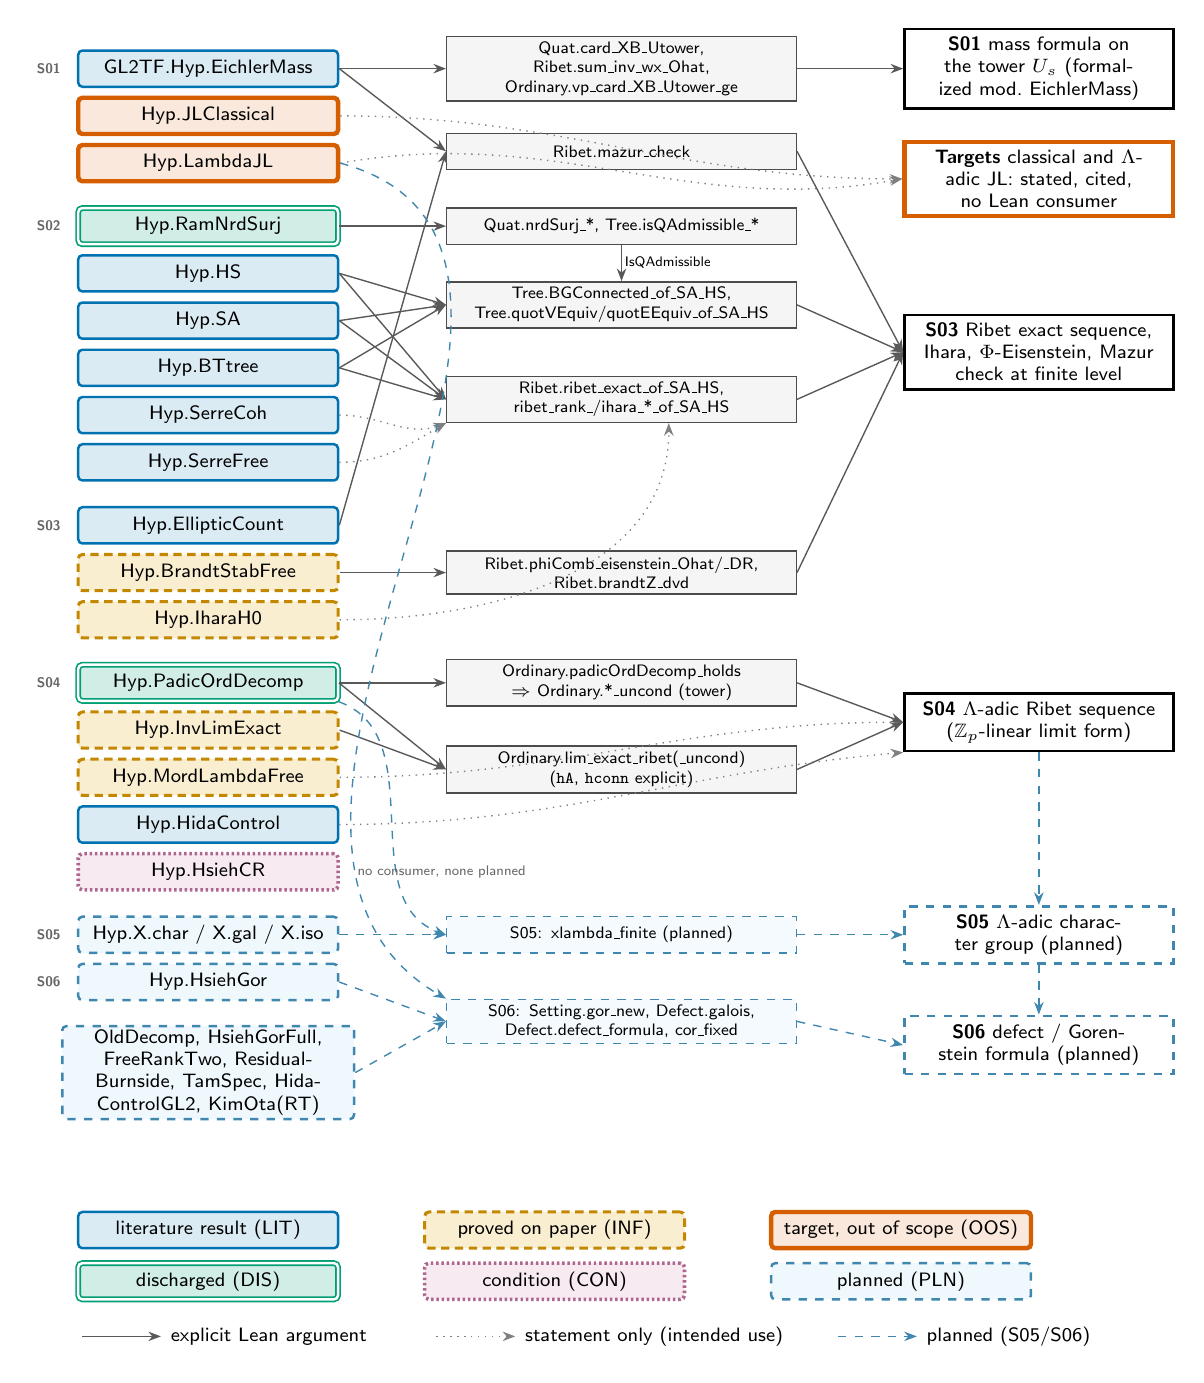
\begin{tikzpicture}[
    x=1cm,y=1cm,font=\sffamily\scriptsize,
    every node/.style={align=center},
    hyp/.style={rectangle,rounded corners=1.5pt,minimum width=3.3cm,minimum height=0.46cm,inner sep=1.5pt,line width=0.9pt},
    lit/.style={hyp,draw=oiBlue,fill=oiBlue!14},
    dis/.style={hyp,draw=oiGreen,fill=oiGreen!18,double,double distance=0.9pt,line width=0.6pt},
    inf/.style={hyp,draw=oiOrange!85!black,fill=oiOrange!18,densely dashed,line width=1.1pt},
    oos/.style={hyp,draw=oiVerm,fill=oiVerm!14,line width=1.6pt},
    con/.style={hyp,draw=oiPurple!85!black,fill=oiPurple!16,densely dotted,line width=1.3pt},
    pln/.style={hyp,draw=oiSky!75!black,fill=oiSky!10,dashed,line width=0.9pt},
    thm/.style={rectangle,draw=black!70,fill=black!4,text width=4.3cm,minimum height=0.46cm,inner sep=2pt,line width=0.5pt,font=\sffamily\fontsize{6}{7}\selectfont},
    plt/.style={thm,dashed,draw=oiSky!75!black,fill=oiSky!6},
    fin/.style={rectangle,draw=black,fill=white,minimum width=3.4cm,inner sep=3pt,line width=1pt,text width=3.2cm},
    pfin/.style={fin,dashed,draw=oiSky!75!black},
    use/.style={-{Stealth[length=1.6mm]},line width=0.5pt,draw=black!65},
    puse/.style={use,dashed,draw=oiSky!75!black},
    intd/.style={use,dotted,draw=black!50},
    stg/.style={font=\sffamily\bfseries\tiny,text=black!60,anchor=east},
  ]
  \def\hx{0}
  \node[lit] (EM)  at (\hx,0)     {GL2TF.Hyp.EichlerMass};
  \node[oos] (JLC) at (\hx,-0.6)  {Hyp.JLClassical};
  \node[oos] (LJL) at (\hx,-1.2)  {Hyp.LambdaJL};
  \node[dis] (RN)  at (\hx,-2.0)  {Hyp.RamNrdSurj};
  \node[lit] (HS)  at (\hx,-2.6)  {Hyp.HS};
  \node[lit] (SA)  at (\hx,-3.2)  {Hyp.SA};
  \node[lit] (BT)  at (\hx,-3.8)  {Hyp.BTtree};
  \node[lit] (SC)  at (\hx,-4.4)  {Hyp.SerreCoh};
  \node[lit] (SF)  at (\hx,-5.0)  {Hyp.SerreFree};
  \node[lit] (EC)  at (\hx,-5.8)  {Hyp.EllipticCount};
  \node[inf] (BSF) at (\hx,-6.4)  {Hyp.BrandtStabFree};
  \node[inf] (IH)  at (\hx,-7.0)  {Hyp.IharaH0};
  \node[dis] (POD) at (\hx,-7.8)  {Hyp.PadicOrdDecomp};
  \node[inf] (ILE) at (\hx,-8.4)  {Hyp.InvLimExact};
  \node[inf] (MLF) at (\hx,-9.0)  {Hyp.MordLambdaFree};
  \node[lit] (HC)  at (\hx,-9.6)  {Hyp.HidaControl};
  \node[con] (CR)  at (\hx,-10.2) {Hyp.HsiehCR};
  \node[pln] (XC)  at (\hx,-11.0) {Hyp.X.char / X.gal / X.iso};
  \node[pln] (HG)  at (\hx,-11.6) {Hyp.HsiehGor};
  \node[pln,text width=3.6cm] (S6) at (\hx,-12.75)
     {OldDecomp, HsiehGorFull, FreeRankTwo, ResidualBurnside, TamSpec, HidaControlGL2, KimOta(RT)};
  \foreach \n/\y in {S01/0,S02/-2.0,S03/-5.8,S04/-7.8,S05/-11.0,S06/-11.6}{\node[stg] at (-1.75,\y) {\n};}

  \def\tx{5.25}
  \node[thm] (tMass) at (\tx,0)     {Quat.card\_XB\_Utower,\\ Ribet.sum\_inv\_wx\_Ohat,\\ Ordinary.vp\_card\_XB\_Utower\_ge};
  \node[thm] (tMaz)  at (\tx,-1.05) {Ribet.mazur\_check};
  \node[thm] (tNrd)  at (\tx,-2.0)  {Quat.nrdSurj\_*, Tree.isQAdmissible\_*};
  \node[thm] (tBG)   at (\tx,-3.0)  {Tree.BGConnected\_of\_SA\_HS,\\ Tree.quotVEquiv/quotEEquiv\_of\_SA\_HS};
  \node[thm] (tRib)  at (\tx,-4.2)  {Ribet.ribet\_exact\_of\_SA\_HS,\\ ribet\_rank\_/ihara\_*\_of\_SA\_HS};
  \node[thm] (tPhi)  at (\tx,-6.4)  {Ribet.phiComb\_eisenstein\_Ohat/\_DR,\\ Ribet.brandtZ\_dvd};
  \node[thm] (tPOD)  at (\tx,-7.8)  {Ordinary.padicOrdDecomp\_holds\\ $\Rightarrow$ Ordinary.*\_uncond (tower)};
  \node[thm] (tLim)  at (\tx,-8.9)  {Ordinary.lim\_exact\_ribet(\_uncond)\\ (\texttt{hA}, \texttt{hconn} explicit)};
  \node[plt] (tXl)   at (\tx,-11.0) {S05: xlambda\_finite (planned)};
  \node[plt] (tDef)  at (\tx,-12.1) {S06: Setting.gor\_new, Defect.galois,\\ Defect.defect\_formula, cor\_fixed};

  \def\fx{10.55}
  \node[fin] (F1) at (\fx,0.0)  {\textbf{S01} mass formula on the tower $U_s$ (formalized mod.\ EichlerMass)};
  \node[fin] (F3) at (\fx,-3.6) {\textbf{S03} Ribet exact sequence, Ihara, $\Phi$-Eisenstein, Mazur check at finite level};
  \node[fin] (F4) at (\fx,-8.3) {\textbf{S04} $\Lambda$-adic Ribet sequence ($\mathbb Z_p$-linear limit form)};
  \node[pfin] (F5) at (\fx,-11.0) {\textbf{S05} $\Lambda$-adic character group (planned)};
  \node[pfin] (F6) at (\fx,-12.4) {\textbf{S06} defect / Gorenstein formula (planned)};
  \node[fin,draw=oiVerm,line width=1.6pt] (FT) at (\fx,-1.4) {\textbf{Targets} classical and $\Lambda$-adic JL: stated, cited, no Lean consumer};

  \draw[use] (EM.east) -- (tMass.west);
  \draw[use] (EM.east) -- (tMaz.west);
  \draw[use] (EC.east) -- (tMaz.west);
  \draw[use] (RN.east) -- (tNrd.west);
  \draw[use] (HS.east) -- (tBG.west);
  \draw[use] (SA.east) -- (tBG.west);
  \draw[use] (BT.east) -- (tBG.west);
  \draw[use] (HS.east) -- (tRib.west);
  \draw[use] (SA.east) -- (tRib.west);
  \draw[use] (BT.east) -- (tRib.west);
  \draw[use] (tNrd.south) -- node[right,font=\sffamily\tiny,inner sep=1pt]{IsQAdmissible} (tBG.north);
  \draw[use] (BSF.east) -- (tPhi.west);
  \draw[use] (POD.east) -- (tPOD.west);
  \draw[use] (POD.east) -- (tLim.west);
  \draw[use] (ILE.east) -- (tLim.west);
  \draw[intd] (SC.east) to[out=0,in=200] (tRib.south west);
  \draw[intd] (SF.east) to[out=0,in=210] (tRib.south west);
  \draw[intd] (IH.east) to[out=0,in=-90] ($(tRib.south)+(0.6,0)$);
  \draw[intd] (MLF.east) to[out=0,in=180] (F4.west);
  \draw[intd] (HC.east) to[out=0,in=185] (F4.south west);
  \draw[intd] (JLC.east) to[out=0,in=180] (FT.west);
  \draw[intd] (LJL.east) to[out=10,in=190] (FT.west);
  \draw[puse] (XC.east) -- (tXl.west);
  \draw[puse] (POD.south east) to[out=-20,in=160] (tXl.west);
  \draw[puse] (HG.east) -- (tDef.west);
  \draw[puse] (S6.east) -- (tDef.west);
  \draw[puse] (LJL.east) to[out=-15,in=150] (tDef.north west);
  \node[font=\sffamily\tiny,anchor=west,text=black!60] at ($(CR.east)+(0.1,0)$) {no consumer, none planned};
  \draw[use] (tMass.east) -- (F1.west);
  \draw[use] (tMaz.east) -- (F3.west);
  \draw[use] (tBG.east) -- (F3.west);
  \draw[use] (tRib.east) -- (F3.west);
  \draw[use] (tPhi.east) -- (F3.west);
  \draw[use] (tPOD.east) -- (F4.west);
  \draw[use] (tLim.east) -- (F4.west);
  \draw[puse] (tXl.east) -- (F5.west);
  \draw[puse] (tDef.east) -- (F6.west);
  \draw[puse] (F4.south) -- (F5.north);
  \draw[puse] (F5.south) -- (F6.north);

  \begin{scope}[shift={(0,-14.75)},every node/.append style={minimum width=3.4cm}]
    \node[lit] at (0.0,0) {literature result (LIT)};
    \node[inf] at (4.4,0) {proved on paper (INF)};
    \node[oos] at (8.8,0) {target, out of scope (OOS)};
    \node[dis] at (0.0,-0.65) {discharged (DIS)};
    \node[con] at (4.4,-0.65) {condition (CON)};
    \node[pln] at (8.8,-0.65) {planned (PLN)};
  \end{scope}
  \begin{scope}[shift={(0,-16.1)}]
    \draw[use] (-1.6,0) -- ++(1,0) node[right,black]{explicit Lean argument};
    \draw[intd] (2.9,0) -- ++(1,0) node[right,black]{statement only (intended use)};
    \draw[puse] (8.0,0) -- ++(1,0) node[right,black]{planned (S05/S06)};
  \end{scope}
\end{tikzpicture}}
\caption{Which hypotheses feed which theorems. Left: registered and planned hypotheses (colour and border style both
encode the kind). Middle: the Lean theorems that take them as arguments. Right: the stage-level statements. Solid
arrows are explicit Lean arguments at \lname{cd0a268}; dotted arrows join a statement-only hypothesis (no library
consumer) to the result it belongs to; dashed arrows are planned. \lname{Hyp.RamNrdSurj} (now discharged by
\lname{Hyp.ramNrdSurj\_holds}) enters every \lname{\_of\_SA\_HS} result at the standard levels through \lname{Tree.isQAdmissible\_*}. \lname{Hyp.InvLimExact} reaches
\lname{lim\_exact\_ribet} only through its conclusion (argument \lname{hA}, supplied as \lname{hI hconn});
\lname{Hyp.LambdaJL} is the only existing hypothesis reused in stage~6.}
\label{fig:hyp-deps}
\end{figure}

\begin{figure}[htbp]\centering
\resizebox{\textwidth}{!}{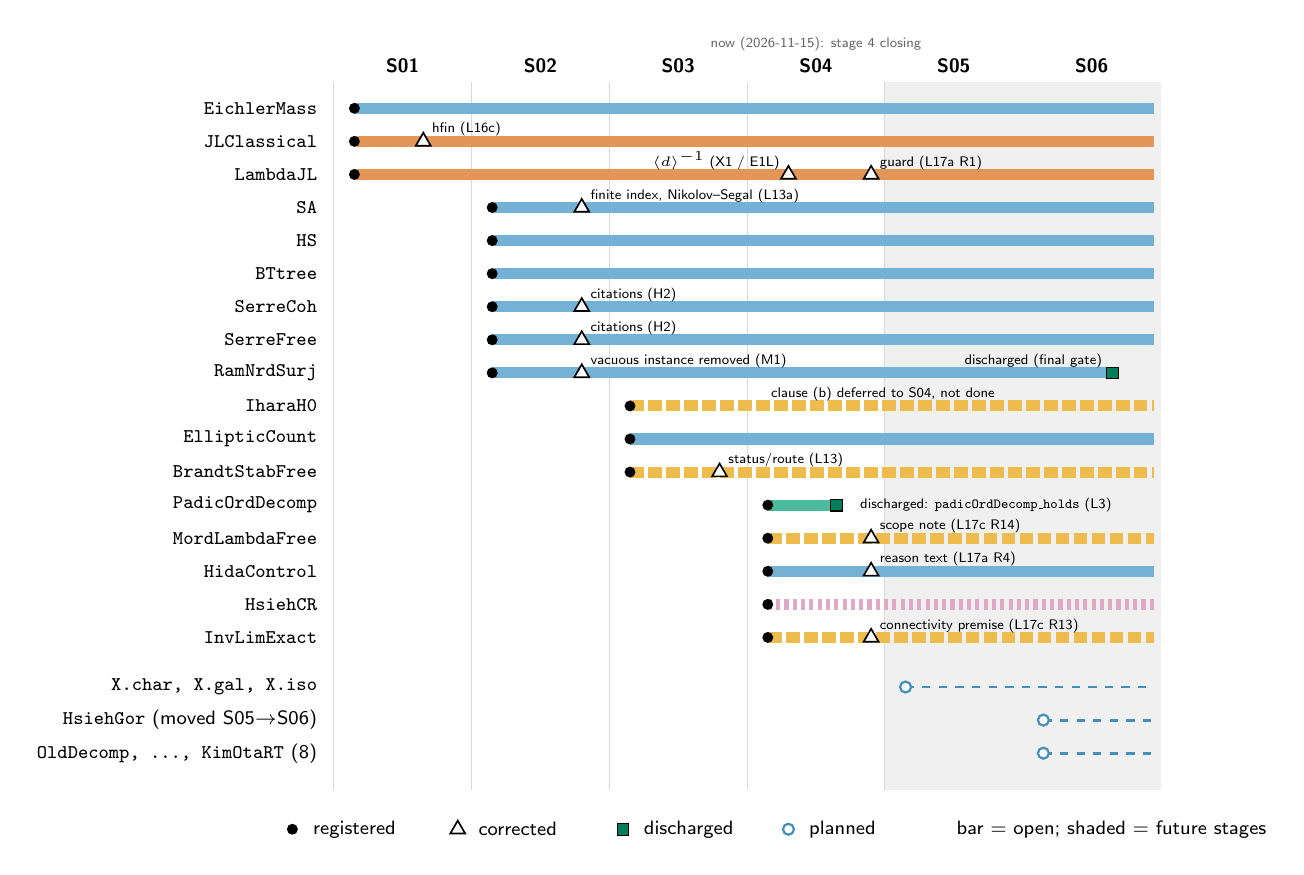
\begin{tikzpicture}[x=1.75cm,y=0.42cm,font=\sffamily\scriptsize]
  \tikzset{
    bar/.style={line width=4pt,line cap=butt},
    lit/.style={bar,draw=oiBlue!55},
    inf/.style={bar,draw=oiOrange!70,dash pattern=on 5pt off 1.5pt},
    oos/.style={bar,draw=oiVerm!65},
    con/.style={bar,draw=oiPurple!65,dash pattern=on 1.5pt off 1.5pt},
    dis/.style={bar,draw=oiGreen!70},
    pln/.style={line width=1pt,draw=oiSky!80!black,dashed},
    intro/.style={circle,fill=black,inner sep=1.4pt},
    corr/.style={regular polygon,regular polygon sides=3,fill=white,draw=black,inner sep=1.1pt,line width=0.6pt},
    disc/.style={rectangle,fill=oiGreen!80!black,draw=black,inner sep=2.1pt},
    plan/.style={circle,draw=oiSky!80!black,fill=white,inner sep=1.4pt,line width=0.8pt},
  }
  \foreach \k in {1,...,6}{
    \draw[black!15] (\k-0.5,0.8) -- (\k-0.5,-20.6);
    \node[font=\sffamily\bfseries\scriptsize] at (\k,1.3) {S0\k};
  }
  \draw[black!15] (6.5,0.8) -- (6.5,-20.6);
  \node[font=\sffamily\tiny,text=black!60] at (4,1.95) {now (2026-11-15): stage 4 closing};
  \fill[black!6] (4.5,0.8) rectangle (6.5,-20.6);
  \def\row#1#2#3#4#5{% #1 y, #2 name, #3 style, #4 start, #5 end
    \node[anchor=east] at (0.45,#1) {\texttt{#2}};
    \draw[#3] (#4-0.35,#1) -- (#5,#1);
    \node[intro] at (#4-0.35,#1) {};}
  \row{0}{EichlerMass}{lit}{1}{6.45}
  \row{-1}{JLClassical}{oos}{1}{6.45}
  \row{-2}{LambdaJL}{oos}{1}{6.45}
  \row{-3}{SA}{lit}{2}{6.45}
  \row{-4}{HS}{lit}{2}{6.45}
  \row{-5}{BTtree}{lit}{2}{6.45}
  \row{-6}{SerreCoh}{lit}{2}{6.45}
  \row{-7}{SerreFree}{lit}{2}{6.45}
  \row{-8}{RamNrdSurj}{lit}{2}{6.15}
  \row{-9}{IharaH0}{inf}{3}{6.45}
  \row{-10}{EllipticCount}{lit}{3}{6.45}
  \row{-11}{BrandtStabFree}{inf}{3}{6.45}
  \row{-12}{PadicOrdDecomp}{dis}{4}{4.15}
  \row{-13}{MordLambdaFree}{inf}{4}{6.45}
  \row{-14}{HidaControl}{lit}{4}{6.45}
  \row{-15}{HsiehCR}{con}{4}{6.45}
  \row{-16}{InvLimExact}{inf}{4}{6.45}
  \node[anchor=east] at (0.45,-17.5) {\texttt{X.char, X.gal, X.iso}};
  \draw[pln] (4.65,-17.5) -- (6.45,-17.5); \node[plan] at (4.65,-17.5) {};
  \node[anchor=east] at (0.45,-18.5) {\texttt{HsiehGor} (moved S05$\to$S06)};
  \draw[pln] (5.65,-18.5) -- (6.45,-18.5); \node[plan] at (5.65,-18.5) {};
  \node[anchor=east] at (0.45,-19.5) {\texttt{OldDecomp, \dots, KimOtaRT} (8)};
  \draw[pln] (5.65,-19.5) -- (6.45,-19.5); \node[plan] at (5.65,-19.5) {};
  \def\ev#1#2#3{\node[corr] at (#1,#2) {}; \node[font=\sffamily\tiny,anchor=south west,inner sep=1pt] at (#1+0.04,#2+0.05) {#3};}
  \ev{1.15}{-1}{hfin (L16c)}
  \node[corr] at (3.8,-2) {}; \node[font=\sffamily\tiny,anchor=south east,inner sep=1pt] at (3.76,-1.95) {$\langle d\rangle^{-1}$ (X1 / E1L)};
  \ev{4.4}{-2}{guard (L17a R1)}
  \ev{2.3}{-3}{finite index, Nikolov--Segal (L13a)}
  \ev{2.3}{-6}{citations (H2)}
  \ev{2.3}{-7}{citations (H2)}
  \ev{2.3}{-8}{vacuous instance removed (M1)}
  \node[disc] at (6.15,-8) {}; \node[font=\sffamily\tiny,anchor=south east,inner sep=1pt] at (6.1,-7.95) {discharged (final gate)};
  \ev{3.3}{-11}{status/route (L13)}
  \node[disc] at (4.15,-12) {}; \node[font=\sffamily\tiny,anchor=west] at (4.25,-12) {discharged: \texttt{padicOrdDecomp\_holds} (L3)};
  \ev{4.4}{-13}{scope note (L17c R14)}
  \ev{4.4}{-14}{reason text (L17a R4)}
  \ev{4.4}{-16}{connectivity premise (L17c R13)}
  \node[font=\sffamily\tiny,anchor=south west,inner sep=1pt] at (3.65,-8.95) {clause (b) deferred to S04, not done};
  \begin{scope}[shift={(0.2,-21.8)}]
    \node[intro] at (0,0) {}; \node[anchor=west] at (0.08,0) {registered};
    \node[corr] at (1.2,0) {}; \node[anchor=west] at (1.28,0) {corrected};
    \node[disc] at (2.4,0) {}; \node[anchor=west] at (2.48,0) {discharged};
    \node[plan] at (3.6,0) {}; \node[anchor=west] at (3.68,0) {planned};
    \node[anchor=west] at (4.75,0) {bar = open; shaded = future stages};
  \end{scope}
\end{tikzpicture}}
\caption{Stage map: when each hypothesis was registered, corrected and discharged (stages 1--4), and what is
planned (stages 5--6). Bar colour and pattern encode the kind, as in Figure~\ref{fig:hyp-deps}; labels name the work package or audit item; details in the entries.}
\label{fig:hyp-timeline}
\end{figure}

\subsection{The hypotheses, one by one}\label{sec:hyp-entries}

Each entry gives: the informal statement; the Lean name and file (relative to \lname{lean/Langlandscape/}); the kind
and source; where it is used (Lean declarations, chapter labels); the current status; what would discharge it; and its
history. Chapter labels refer to \lname{mathematics/chapters/}.

\subsubsection{Stage 1: targets and the mass formula}

\begin{hypentry}{GL2TF.Hyp.EichlerMass}{\kindlit}{S01 (reused from the import)}
\item[Statement] For a maximal order $\cO$ of $B=(a,b)_\Q$ that is ramified exactly at the primes dividing $D$:
  $\operatorname{mass}(\cO)=\sum_{[I]} 1/|\cO_\ell(I)^\times| = \frac{1}{24}\prod_{p\mid D}(p-1)$ (Eichler's mass formula,
  full unit groups). The ramification datum is an antecedent, so the family is true for every index.
\item[Lean] \lname{GL2TF.Hyp.EichlerMass a b D O} in
  \lname{trace-formula-project-import/lean/AlgJL/Hyp/EichlerMass.lean} (tag \lname{III.qcls.hyp:eichler-mass});
  alias \lname{Langlandscape.Hyp.EichlerMass} (\lname{Hyp/JLClassical.lean}, an \lname{abbrev}).
\item[Source] \emph{cited}: Eichler \cite{Eic55}; Shimizu \cite[(20)--(21), p.~180]{Shz65}; Pizer
  \cite[P0.5]{Piz80}; Voight \cite{Vo}. Chapter: \lname{thm:s01-mass}(a), \lname{if:s01-mass}.
\item[Used by] \lname{Quat.card\_XB\_Utower} (\lname{thm:s01-mass}(c),(d)), \lname{Smoke.eichlerMass\_apply},
  \lname{Ribet.sum\_inv\_wx\_Ohat}, \lname{Ribet.mazur\_check} (\lname{prop:s03-mazur}),
  \lname{Ordinary.vp\_card\_XB\_Utower\_ge} (stage 4). (Registry updated at S05-E1, item~\ref{inc:usedby}.)
\item[Status] Open in this project. Closed instances exist in the import's \emph{test} library
  (\lname{GL2TFTests.eichlerMass\_d11}, mass $5/12$; \lname{GL2TFTests.eichlerMass\_d2}, Hurwitz order, mass $1/24$),
  which is not a dependency of \lname{lean/Langlandscape/}; non-vacuity is therefore shown, but the instances cannot be
  used from our code.
\item[Discharge] In the import's plan: chapter III.13 (``Q8'') of the GL(2) trace-formula project, i.e.\ the
  Eichler mass formula from the trace formula / zeta functions of $B$. Not planned here.
\item[History] Unchanged since S01; reused, never redefined.
\end{hypentry}

\begin{hypentry}{Hyp.JLClassical}{\kindoos}{S01-L13}
\item[Statement] Classical Jacquet--Langlands for $k=2$, trivial coefficients: for $M$ prime to $D$ there is an
  isomorphism $\C^{X_B(U_0(M))}\cong S_2(\Gamma_0(DM))^{D\text{-new}}\oplus\C\cdot\mathrm{Eis}$ intertwining $T_\ell$ for
  all primes $\ell\nmid DM$ ($T_\ell$ acts on the Eisenstein line by $\ell+1$).
\item[Lean] \lname{Hyp.JLClassical d M hM S} in \lname{Hyp/JLClassical.lean}; the GL$_2$ side is abstract data
  \lname{S : GL2CuspData (D*M) 2} (a finite-dimensional $\C$-space with commuting operators), because Mathlib v4.35 has
  neither $S_k(\Gamma_0(N))$ with Hecke operators nor the comparison. With arbitrary \lname{S} the proposition only says
  that \lname{S} is a Hecke-module complement of the constants: it has no GL$_2$ content (\emph{schematic}, F6).
\item[Source] \emph{cited}: Jacquet--Langlands \cite{JL}; Gross \cite{Gr99}. Chapter: \lname{thm:s01-JLclassical}
  (\stcited; \lname{\textbackslash lean} mark ``schematic interface'').
\item[Used by] No Lean consumer; it is a target statement.
\item[Status] Open (schematic); no instance (none is feasible without GL$_2$ Hecke theory).
\item[Discharge] Not discharged during the event; planned for Stage~2 via the GL(2) trace-formula formalization (route~1 of
  \lname{ss:s00-whycited}), timing uncertain (see the report's Stage-2 plan). It would also remove the JL input to the comparison
  beyond $D=q$ (the Shimura-curve version of \lname{Hyp.X}), provided the trace-formula comparison is carried out for the quaternion algebra occurring there. It needs the classical JL correspondence formalized, e.g.\ via a complete GL(2) trace
  formula and its comparison with the quaternionic side (the import provides part of the trace formula, not the
  comparison), together with Hecke operators on $S_2(\Gamma_0(N))$ in Mathlib.
\item[History] S01 Lean audit R1/R9: the finiteness premise \lname{hfin} of $T_\ell$ was universally quantified
  and unprovable; discharged by \lname{relIndex\_elemT\_ne\_zero\_U0} (S01-L16c, \lname{6f229dc8}). Its docstring now cites the
  \lname{mathematics/} label (S05-E1, item~\ref{inc:planstaged}).
\end{hypentry}

\begin{hypentry}{Hyp.LambdaJL}{\kindoos}{S01-L13}
\item[Statement] $\Lambda$-adic Jacquet--Langlands: a surjection of $\Lambda$-algebras
  $\varphi:\T^{\mathrm{ord}}_{\mathrm{GL}_2}\to\T^{\mathrm{ord}}_B$ with kernel the $D$-new ideal, matching
  $T_\ell\mapsto T_\ell$ ($\ell\nmid DMp$), $U_\ell\mapsto U_\ell$ ($\ell\mid Mp$), $U_\ell\mapsto\Pi_\ell$ ($\ell\mid D$),
  and the diamonds by \emph{classical $\langle d\rangle\mapsto$ seed $\langle d\rangle^{-1}$}, for $d$ prime to $Mp$.
\item[Lean] \lname{Hyp.LambdaJL D M p Λ TGL TB genGL genB newIdeal} in \lname{Hyp/LambdaJL.lean}; both Hecke
  algebras, their generators and the new ideal are abstract (\emph{schematic}). The diamond clause is
  \lname{∀ d, Nat.Coprime d (M*p) → φ (genGL (.dia d)) * genB (.dia d) = 1}.
\item[Source] \emph{cited}: Chenevier \cite{Ch}; Longo--Vigni \cite[Prop.~6.1]{LV}; Hsieh \cite[\S4.5]{Hs}.
  Chapter: \lname{thm:s01-lambdaJL}, \lname{rem:s01-diamond}, \lname{lem:s01-Upconv}, \lname{if:s01-targets}.
\item[Used by] \lname{Defect.Setting.gor\_new}, \lname{Defect.defect\_formula}, \lname{Defect.cor\_allweights} (explicit
  argument \lname{hJL}; stage 6; only surjectivity and the kernel are used); otherwise a target statement, schematic.
\item[Status] Open (schematic); no instance.
\item[Discharge] Not during the event: needs classical JL plus Hida theory on the GL$_2$ side; its classical input could come
  from route~1 (\lname{ss:s00-whycited}; the Stage-2 plan: ``possibly the classical input of \lname{LambdaJL}''). Stage~06 takes it
  as a cited input because it does not use \lname{Hyp.X}.
\item[History, corrections] (1) \textbf{Inverse diamond (X1 erratum).} The original clause
  $\varphi(\langle d\rangle_{\mathrm{GL}})=\langle d\rangle_B$ encoded a false matching: the seed's adelic
  $\langle d\rangle$ is the classical $\langle d\rangle^{-1}$ (\lname{rem:s01-diamond}). Found by the blind cross-account
  review (\lname{mathematics/audits/2026-11-14\_s01-xacct.md}, item X1, \emph{major}; the S01 Lean audit had missed
  it); fixed in the chapter by S04-E1M (\lname{65b8f55c}) and in Lean by S04-E1L (\lname{6acc2ab9}), stated as
  $\varphi\langle d\rangle_{\mathrm{GL}}\cdot\langle d\rangle_B=1$. (2) \textbf{Coprimality guard.} The unguarded unit
  condition forced $0=1$ at the junk value $\langle 0\rangle=0$, making the hypothesis unsatisfiable (S04 Lean audit,
  R1); S04-L17a (\lname{7f984fa3}) added \lname{Nat.Coprime d (M*p)}. The chapter now states the guard (S05-E1, item~\ref{inc:guard}).
\end{hypentry}

\subsubsection{Stage 2: strong approximation, norms, trees}

\begin{hypentry}{Hyp.SA}{\kindlit}{S02-L4a}
\item[Statement] Strong approximation for $B^1$ at $S=\{\infty,q\}$, in the shape (SA$_U$): for every $q$-admissible
  level $U$, $\hat B^1=B^1\,(B^1_q\times U^{1,(q)})$.
\item[Lean] \lname{Hyp.SA d q hq := ∀ U, Tree.IsQAdmissible d q hq U → Tree.SAat d q hq U} in \lname{Hyp/SA.lean}.
\item[Source] \emph{cited}: Voight \cite[Main Thm.~28.5.3, Cor.~28.5.12]{Vo}; Vign\'eras \cite[III.4.3]{Vigneras1980};
  for finite-index (not necessarily open) levels also Nikolov--Segal \cite[Thm.~1.1]{NS07}. Chapter: \lname{thm:s02-SA}.
\item[Used by] \lname{Tree.BGConnected\_of\_SA\_HS}, \lname{Tree.surjType0\_of\_SA\_HS},
  \lname{quotVEquiv\_of\_SA\_HS}, \lname{quotEEquiv\_of\_SA\_HS}, \lname{quotEquiv\_oO/\_tO\_of\_SA\_HS}
  (\lname{prop:s02-BG}, \lname{prop:s02-quot}); and \lname{Ribet.ribet\_exact\_of\_SA\_HS},
  \lname{ribet\_rank\_of\_SA\_HS}, \lname{ihara\_surj\_of\_SA\_HS}, \lname{ihara\_ker\_const\_of\_SA\_HS}
  (\lname{thm:s03-ribet}, \lname{cor:s03-ihara}); the last four are missing from the registry.
\item[Status] Open; no instance. Per level it is replaced by the connectivity premise \lname{BGConnected}
  (\lname{prop:s02-BG}), which the \lname{\_uncond} stage-4 results take directly.
\item[Discharge] Strong approximation for $\mathrm{SL}_1(B)$ over $\Q$ (plan item L02.SA, post-hackathon); needs adelic
  algebraic groups in Mathlib. The import has a \lname{strong\_approximation} for GL$_2$ that does not cover $B^1$.
\item[History] S02 Lean audit: \lname{IsQAdmissible} says ``finite index'' where the tex says ``compact open'';
  the openness step via Nikolov--Segal was added to the docstring (S02-L13a, \lname{faf256dd}). For the project's levels
  ($\hat\cO^\times$, $U_0(N)$, $U_1(N)$, $U_s$, all open) Nikolov--Segal is not needed.
\end{hypentry}

\begin{hypentry}{Hyp.HS}{\kindlit}{S02-L4a}
\item[Statement] Hasse--Schilling for the definite algebra: every positive rational is the reduced norm of a unit of
  $B$, $\Nrd(B^\times)=\Q_{>0}$ (the inclusion $\subseteq$ is proved).
\item[Lean] \lname{Hyp.HS d := ∀ r : ℚ, 0 < r → ∃ γ : (QuatAlg ℚ d.a d.b)ˣ, nrd γ = r} in \lname{Hyp/HS.lean}.
\item[Source] \emph{cited}: Voight \cite[Main Thm.~14.7.4]{Vo}; Vign\'eras \cite[III.4.1]{Vigneras1980}. Chapter:
  \lname{lem:s02-normone}(b).
\item[Used by] \lname{Tree.XBone\_toXB\_bijective} and all \lname{\_of\_SA\_HS} results listed under \lname{Hyp.SA}.
\item[Status] Open; no instance.
\item[Discharge] Hasse--Schilling, i.e.\ the Hasse--Minkowski theorem for the ternary norm form (post-hackathon);
  needs Hasse--Minkowski over $\Q$ in Mathlib.
\item[History] Unchanged.
\end{hypentry}

\begin{hypentry}{Hyp.BTtree}{\kindlit}{S02-L5b}
\item[Statement] The coset graph on $\GL_2(\Q_q)/\Q_q^\times\GL_2(\Z_q)$ is a tree in which every vertex has $q+1$
  neighbours (the Bruhat--Tits tree). Only connectedness is used downstream.
\item[Lean] \lname{Hyp.BTtree q := (Tree.graph q).IsTree ∧ ∀ v, Nat.card (neighborSet v) = q + 1} in
  \lname{Hyp/BTtree.lean}.
\item[Source] \emph{cited}: Serre \cite[II.1.1, Thm.~1]{Se}; formalized (Lean~4, older Mathlib) by Ludwig--Merten
  \cite{LM}. Chapter: \lname{lem:s02-tree}(a).
\item[Used by] \lname{Tree.BGConnected\_of\_surj}, \lname{Tree.BGConnected\_of\_SA\_HS} (step (i)$\Rightarrow$(iii) of
  \lname{prop:s02-BG}) and the four \lname{Ribet.*\_of\_SA\_HS} (all take \lname{hBT}); the registry now lists them.
\item[Status] Open; no instance.
\item[Discharge] Port of the Ludwig--Merten formalization from Lean v4.19 to v4.35 (post-hackathon).
\item[History] S02 audit H6: docstring records that $(q+1)$-regularity is not consumed.
\end{hypentry}

\begin{hypentry}{Hyp.SerreCoh}{\kindlit}{S02-L3}
\item[Statement] If $\BG(U,q)$ is connected and all stabiliser orders $|\Gamma_x|$ are units in $R$, then
  $H_1(\Gamma_U,R)\cong\ker\partial$ and $H_0(\Gamma_U,R)\cong\coker\partial$ for the two-term complex $\partial$ of the
  quotient graph (trivial coefficients).
\item[Lean] \lname{Hyp.SerreCoh d q hq U hU hconn R} in \lname{Hyp/SerreCoh.lean} (Mathlib \lname{groupHomology};
  $R$ in \lname{Type} for universe reasons; the isomorphisms are abstract, not asserted compatible with $\partial$).
\item[Source] \emph{cited}: Serre \cite[II.2.8, Prop.~13 and Rem.~1]{Se}; Brown \cite[VII.7]{Br}. Chapter:
  \lname{prop:s02-coh}(b) (\stpmc; the tex has coefficients $V$, the Lean form trivial coefficients).
\item[Used by] Statement only (test \lname{LanglandscapeTests/S02/SerreShape.lean}).
\item[Status] Open; no instance.
\item[Discharge] Bass--Serre theory (homology of groups acting on trees) in Mathlib (post-hackathon, plan item L02.6).
\item[History] S02 audit H2/H6: citations and docstring corrected.
\end{hypentry}

\begin{hypentry}{Hyp.SerreFree}{\kindlit}{S02-L3}
\item[Statement] If $\BG(U,q)$ is connected and all $\Gamma_x(U)$ are trivial, then $\Gamma_U$ is free of rank
  $(q-1)|X(U)|+1$.
\item[Lean] \lname{Hyp.SerreFree d q hq U hU hconn hfree} in \lname{Hyp/SerreFree.lean} (via
  \lname{FreeGroupBasis}).
\item[Source] \emph{cited}: Serre \cite[I.3.3, Thm.~4$'$; II.1.5, Thm.~4]{Se}; Bass \cite[3.6]{Bass1993}.
  Chapter: \lname{prop:s02-free}(a).
\item[Used by] Statement only (test \lname{SerreShape.lean}).
\item[Status] Open; no instance.
\item[Discharge] Needs \lname{Hyp.BTtree} and Serre's theorem that a group acting freely on a tree is free
  (Bass--Serre theory), post-hackathon.
\item[History] S02 audit H2/H6: citations corrected.
\end{hypentry}

\begin{hypentry}{Hyp.RamNrdSurj}{\kinddis}{S02-L10}
\item[Statement] At every ramified prime $\ell\mid D$, the reduced norm maps the units of the local maximal order onto
  $\Z_\ell^\times$: $\Nrd(\cO_\ell^\times)=\Z_\ell^\times$.
\item[Lean] \lname{Hyp.RamNrdSurj d} in \lname{Hyp/RamNrdSurj.lean}.
\item[Source] \emph{cited}: Voight \cite[Lemma~13.4.9]{Vo}; Vign\'eras \cite[II.1.5]{Vigneras1980}; also proved on paper in
  \lname{lem:s01-nrd} from the cited local structure (Voight Thm.~13.3.11); \emph{formalized} (below). Chapter:
  \lname{lem:s01-nrd} (the $\ell\mid D$ ingredient; status reconciled across s01, s02 and Lean at S05-E1, item~\ref{inc:nrd}).
\item[Used by] \lname{Quat.exists\_Ohat\_nrd\_eq}, \lname{Quat.nrdSurj\_Ohat}, \lname{nrdSurj\_U0}, \lname{nrdSurj\_U1},
  \lname{nrdSurj\_Utower}; \lname{Tree.isQAdmissible\_Ohat}, \lname{\_U0}, \lname{\_U1}, \lname{\_Utower}. Hence, at the
  standard levels, every \lname{\_of\_SA\_HS} consumer.
\item[Status] \textbf{Discharged} by \lname{Langlandscape.Hyp.ramNrdSurj\_holds (d : DefiniteData) : Hyp.RamNrdSurj d}
  (\lname{Hyp/RamNrdSurjDischarge.lean}), via the reduction \lname{Hyp.ramNrdSurj\_of\_local} and the local inputs
  \lname{Local.exists\_nrd\_eq\_unit\_of\_ne\_two} (\lname{Local/QuatNrdOdd.lean}) and \lname{Local.exists\_nrd\_eq\_unit\_two}
  (\lname{Local/QuatNrdTwo.lean}); all four use only \lname{propext}, \lname{Classical.choice}, \lname{Quot.sound}
  (final gate, build machine A \lname{ramnrd-final-2} at \lname{2323a252}). The consumers keep the explicit argument and receive it
  as \lname{ramNrdSurj\_holds d}. Needed for every definite algebra ($D>1$ always).
\item[Discharge] Done (2026-11-15) by a route different from the chapter's: the local inputs show that every
  $w\in\Z_\ell^\times$ is a reduced norm from $(a,b\mid\Q_\ell)$ at \emph{every} prime $\ell$ and for all nonzero $a,b$
  (\emph{formalized}, the two \lname{Local} theorems); $\ell\mid D$ enters only through $\cO_\ell=\{x:\Nrd x\in\Z_\ell\}$.
  The proof was drafted by an external model (mistral-large-4-0 via opencode), outside our agent process; see the
  final report, \S3.
\item[History] Introduced as a deviation of S02-L10. Its only instance, for $D=1$, was vacuous (no definite algebra
  has $D=1$; S02 audit M1) and was deleted (S02-L13a, \lname{faf256dd}). Discharged after the S06 gate (merge
  \lname{2323a252}; independent Fable audit PASS WITH REMARKS).
\end{hypentry}

\subsubsection{Stage 3: Ribet's sequence, Ihara, Mazur}

\begin{hypentry}{Hyp.IharaH0}{\kindinfra}{S03-L11}
\item[Statement] Ihara's lemma with coefficients, clause (a): under the standing hypotheses of \lname{ss:s03-ihara}
  ($p\ge5$, $p\ne q$, $p\nmid D$, $U$ $q$-admissible and factorisable at $p$, $\BG(U,q)$ connected, $V$ a f.g.\
  $\Z_p$-module with continuous $U_p$-action, $-1$ acting trivially), the map
  $\varepsilon:\Brandt{U}{V}^2\to V_{U^1_p}$ is well defined and onto, and $\ker\varepsilon=\operatorname{im}\alpha$ for
  $\alpha=(-s_{0*},s_{1*})$; hence $\coker\alpha\cong V_{U^1_p}$.
\item[Lean] \lname{Hyp.IharaH0 d q hq U hU p hp V c} in \lname{Hyp/IharaH0.lean}.
\item[Source] \emph{proved modulo cited} in the chapter (\lname{thm:s03-iharaH0}(a), \stpmc): well-definedness,
  $\varepsilon\circ\alpha=0$ and surjectivity are elementary; only $\ker\varepsilon\subseteq\operatorname{im}\alpha$
  uses the density of $\Gamma_U$ in $U^1_p$ (full strong approximation, \lname{cor:s03-ihara}(ii$'$)). Classical
  analogue: Diamond--Taylor \cite[pp.~445--446]{DT}.
\item[Used by] Statement only (tests; intended for stage-6 mathematics and the talk).
\item[Status] Open; no instance. Premises jointly satisfiable at $\hat\cO^\times$ with trivial $\rho$ (S03 Fable
  audit: not vacuous).
\item[Discharge] Prove the elementary conjuncts now and reduce to $\ker\varepsilon\le\operatorname{range}\alpha$; that
  part needs \lname{Hyp.SA} and the cohomological interface \lname{if:s02-coh}. Post-hackathon.
\item[History] Clause (b) (Hecke action) excluded from the start and deferred as an optional output of S04-L15a,
  which merged without it; the Hecke operators with coefficients ``from S04-L15a'' now exist
  (\lname{Brandt/HeckeCoeff.lean}, \lname{Brandt/UpCoeff.lean}); registry updated at S05-E1 (item~\ref{inc:ihara}), clause (b) still not stated.
\end{hypentry}

\begin{hypentry}{Hyp.EllipticCount}{\kindlit}{S03-L6}
\item[Statement] For $D=q$ prime and $U=\hat\cO^\times$: if $q\ge5$, every class has $w_x\in\{1,2,3\}$, exactly
  $[q\equiv3\bmod4]$ classes have $w_x=2$ and exactly $[q\equiv2\bmod3]$ classes have $w_x=3$; if $q\in\{2,3\}$, then
  $|X_B(\hat\cO^\times)|=1$.
\item[Lean] \lname{Hyp.EllipticCount d} in \lname{Hyp/EllipticCount.lean}.
\item[Source] \emph{cited}: Voight \cite[Thm.~11.5.14, 25.1.1, 30.1.5]{Vo}; Mazur \cite[App., Thm.~1.1(d)]{Mz}.
  Chapter: \lname{lem:s03-elliptic} (\stpmc) and the $q\in\{2,3\}$ part of \lname{prop:s03-mazur}.
\item[Used by] \lname{Ribet.mazur\_check} (with \lname{EichlerMass}; every prime $D$, the $q\le3$ clause included, so the $q=2,3$ Mazur check is formalized modulo this hypothesis; item~\ref{inc:mazur}); tests \lname{test\_mazur\_check\_*}.
\item[Status] Open; no closed instance. True for every prime $D$, hence non-vacuous.
\item[Discharge] The Eichler class number formula and the classification of unit groups of maximal orders; both are
  absent from Mathlib and the import.
\item[History] Cross-account review s03 X6 (Lean stronger than the lemma, because of the $q\in\{2,3\}$ clause):
  resolved by the chapter note.
\end{hypentry}

\begin{hypentry}{Hyp.BrandtStabFree}{\kinddis}{S03-L8}
\item[Statement] At $U=\hat\cO^\times$, for a prime $\ell\nmid D$ and classes $c\ne c'$, the weight $w_c$ divides the
  Brandt matrix entry $B(\ell)_{cc'}$ (the stabiliser $\Gamma_c/\{\pm1\}$ acts freely on the neighbours in a different
  class).
\item[Lean] \lname{Hyp.BrandtStabFree d ℓ} in \lname{Hyp/BrandtStabFree.lean}; it also assumes $D$ prime, which
  the proof does not use, and is stated only at $\hat\cO^\times$ (the tex holds for all levels $U_0(M)$).
\item[Source] \emph{proved} in the chapter (\lname{lem:s03-stabfree}, \stproved, elementary: $\Z[\gamma]$ is $\Z[i]$ or
  $\Z[\omega]$, Euclidean, so $\pi\in\Z[\gamma]$ with $\Nrd\pi=\ell$). Cross-reference: Ribet \cite[Thm.~3.12]{Ri90}.
\item[Used by] \lname{Ribet.phiComb\_eisenstein\_Ohat}, \lname{Ribet.phiComb\_eisenstein\_DR},
  \lname{Ribet.brandtZ\_dvd} (step (1) of \lname{prop:s03-phieis}).
\item[Status] \textbf{Discharged} by \lname{Langlandscape.Hyp.brandtStabFree\_holds}
  (\lname{Hyp/BrandtStabFreeDischarge.lean}): an external draft (mistral-large-4-0 via opencode, on the second team member's machine,
  outside our agent process), integrated into the library, independently audited (Fable, PASS) and gated by our agents.
\item[Discharge] (Plan before the discharge.) The neighbour/lattice description (\lname{lem:s03-nbr}) of the import's Brandt matrix plus the
  arithmetic of $\Z[i],\Z[\omega]$ inside $B$. Working estimate (item~\ref{inc:brandt}): 1000--1500 lines via Morita theory plus a PID argument (probed
  2026-11-14); the 500--800 line elementary route in \lname{STATE.md} is unprobed. The unused premise ``$D$ prime'' is
  recorded in the registry (open design decision). Deferred post-stage-04.
\item[History] Registered with a ``Morita + PID'' source; the S03 Lean audit R1 found the chapter proof elementary;
  status and route corrected in S03-L13 (\lname{e63c5c48}, \lname{fae211a3}).
\end{hypentry}

\subsubsection{Stage 4: Hida theory, control, the $\Lambda$-adic Ribet sequence}

\begin{hypentry}{Hyp.PadicOrdDecomp}{\kinddis}{S04-L1}
\item[Statement] Every endomorphism $T$ of a finitely generated $\Z_p$-module $M$ has an ordinary decomposition
  $M=M^{\mathrm{ord}}\oplus M^{\mathrm{nil}}$ ($T$ invertible on the first summand, topologically nilpotent on the second).
\item[Lean] \lname{Hyp.PadicOrdDecomp p} in \lname{Hyp/PadicOrdDecomp.lean}.
\item[Source] \emph{proved} in the chapter (\lname{def:s04-e}, Step~5) and \emph{formalized}.
\item[Used by] About 25 tower theorems in \lname{Ordinary/\{RibetFinite, RibetFiniteFull, Tower, TowerRank, Limit\}.lean}
  as the argument \lname{hdec}, including \lname{Ordinary.lim\_exact\_ribet}, the L10b theorem \lname{ordFree\_finite} and the L17b
  \lname{RibetFiniteFull} results (item~\ref{inc:usedby}).
\item[Status] \textbf{Discharged} by \lname{Langlandscape.Ordinary.padicOrdDecomp\_holds}
  (\lname{Ordinary/PadicDecomp.lean}, S04-L3, Weierstrass-preparation route; standard axioms only, gate
  \lname{s04-int4b-1}). At \lname{cd0a268} every consumer has an \lname{\_uncond} twin in
  \lname{Ordinary/TowerUncond.lean} (18 theorems, e.g.\ \lname{lim\_exact\_ribet\_uncond},
  \lname{ordRibet\_exact\_Utower\_uncond}, \lname{ord\_control\_finite\_uncond}).
\item[History] Registered at S04-X1 as ``to be proved'' (fallback F-e of the stage plan); discharged in S04-L3
  (\lname{a2326c23}); stale ``to be discharged'' text fixed in L17a (R4); \lname{\_uncond} forms completed in L17b/L17c
  (R9, R11).
\end{hypentry}

\begin{hypentry}{Hyp.InvLimExact}{\kindinfra}{S04-L14b}
\item[Statement] If $\BG(UU_s,q)$ is connected for all $s\ge1$, the transition maps
  $e\,H_1(\Gamma_{UU_{s+1}})\to e\,H_1(\Gamma_{UU_s})$ of the $A$-system of the ordinary Ribet sequence are surjective.
\item[Lean] At \lname{cd0a268}: \lname{Hyp.InvLimExact H := (∀ s ≥ 1, Tree.BGConnected \dots (d.Utower M p s \dots))
  → ∀ n, Function.Surjective (H.transA n)} in \lname{Hyp/InvLimExact.lean}. At \lname{d214fb58} the connectivity
  premise is absent.
\item[Source] \emph{proved} in the chapter (\lname{thm:s04-lambdaribet}(a), \stproved) by the D-lim route: control at
  both levels, $\Delta$-linearity of $\alpha$, snake lemma, under connectivity. The compactness proof in the same theorem
  gives exactness of the limit \emph{without} this surjectivity, so it does not prove this statement.
\item[Used by] \lname{Ordinary.lim\_exact\_ribet} and \lname{lim\_exact\_ribet\_uncond}, but only through their
  argument \lname{hA : ∀ n, Function.Surjective (H.transA n)}, which is supplied as \lname{hI hconn} from
  \lname{hI : Hyp.InvLimExact H} (test \lname{LanglandscapeTests/S04/HypLam.lean}). No library declaration mentions
  \lname{Hyp.InvLimExact} in its type (registry row and chapter corrected at S05-E1, item~\ref{inc:invlim}).
\item[Status] Open (the conditional fallback of S04-L13b); no instance (needs a concrete \lname{RibetHyp}); not
  vacuous.
\item[Discharge] Formalize the D-lim snake route on the concrete Ribet systems: the abstract snake step
  \lname{Ordinary.surjective\_of\_snake} exists; missing are the control kernel $\ker=I\cdot B$ and the
  $\Delta$-equivariance of $\alpha$ (deviation 7 dropped this in stage 4). Connectivity itself follows from
  \lname{Hyp.SA}, \lname{Hyp.HS}, \lname{Hyp.BTtree} (cross-account review s04, X8).
\item[History, corrections] Introduced after the stage-4 plan audit (Muse, F2) found the fallback undeclared.
  \textbf{Connectivity premise added} by S04-L17c (\lname{3013fb81}, audit R13): the tex assumes $\BG(UU_s,q)$ connected
  (global seam audit F7, decision D5; \lname{s04/lambdaribet.tex}, marked \lname{\textbackslash provisional}), and the
  old ``compactness'' justification was wrong. Registry row and chapter updated at S05-E1 (item~\ref{inc:invlim}).
\end{hypentry}

\begin{hypentry}{Hyp.MordLambdaFree}{\kindinfra}{S04-L14b}
\item[Statement] $\Mord(U)=\varprojlim_s e\,\Z_p[X_s(U)]$ is a free $\Lambda$-module of finite rank, and for every $n$
  the projection to level $n+1$ is onto with kernel $\ker(\Lambda\to\Z_p[\Delta_{n+1}])\cdot\Mord(U)$
  (control, $\Lambda$-adic half).
\item[Lean] \lname{Hyp.MordLambdaFree T π ρ hρ} in \lname{Hyp/MordLambdaFree.lean}; the $\Lambda$-module structure
  comes from explicit levelwise diamond data \lname{(ρ, hρ)}. It is the theorem \emph{only} for the intended data
  ($G_n=\Delta_{n+1}$, reduction maps, diamond action); these data do not yet exist in Lean (scope note, R14,
  \lname{cd0a268}). The rank is $\exists r$; Hecke compatibility is not part of the statement.
\item[Source] Chapter \lname{thm:s04-control}(a): \stproved{} (raised from \stpmc{} after S04-M9); also
  \emph{cited}: Hsieh \cite[Thm.~4.2]{Hs}; Longo--Vigni \cite[Prop.~3.6]{LV11}. Lean docstring and registry now say ``tex proved'' (S05-E1, item~\ref{inc:mord}).
\item[Used by] Statement only (test \lname{HypLam.lean}); no consumer is named in the stage-5/6 plans (grep at S05-E1).
\item[Status] Open; no instance (a vacuous one is forbidden); toy case $\Delta_s=1$ described in the docstring only.
\item[Discharge] Build the diamond data, compatible bases $e\,\Z_p[X_s]\cong\Z_p[\Delta_s]^r$ (Nakayama), and the
  Iwasawa algebra; post-stage.
\item[History] Scope note added by L17c (R14).
\end{hypentry}

\begin{hypentry}{Hyp.HidaControl}{\kindlit}{S04-L14a}
\item[Statement] Weight control, definite side, finite level mod $p^s$: for $k\ge2$ and $U=U_1(M)$-type levels with
  $p\nmid\varphi(M)$, the ordinary part of the weight-$k$ Brandt module mod $p^s$ is isomorphic to the ordinary part of
  $e\,\cO[X_s(U)]/P_k$ (\lname{def:s04-Pk}).
\item[Lean] \lname{Hyp.HidaControl M p s k hk hφ A Mk Uk M2 U2 Pk Qk π Ubar} in \lname{Hyp/HidaControl.lean};
  \emph{schematic}: the Hecke modules are abstract data (decision Q3, taken at int3 before the coefficient Hecke
  operators \lname{Brandt/HeckeCoeff.lean}, \lname{UpCoeff.lean} were green). Stated on modules, not on their duals as
  in the tex.
\item[Source] \emph{cited}: Hsieh \cite[Thm.~4.2(2)]{Hs}; Longo--Vigni \cite[Thm.~3.7]{LV11}; Hida
  \cite[Thm.~9.4]{Hi88b}. Chapter: \lname{thm:s04-control}(b), \lname{rem:s04-controlb}.
\item[Used by] Statement only (test).
\item[Status] Open (schematic); no instance (an instance on abstract data would be vacuous).
\item[Discharge] A faithful statement first: $U_p$ on $V_k$-coefficients at all levels $U_s$ (\lname{UpV}, S04-L15b),
  the quotient by $P^{\mathrm{ad}}_k$, and $\Mord$. Cited, post-hackathon.
\item[History] S04 audit R4: the stated reason (``coefficients not available'') was stale; corrected in L17a.
  Open: audit item O1 (\lname{hk} unused; now recorded in registry and chapter, not applied).
\end{hypentry}

\begin{hypentry}{Hyp.HsiehCR}{\kindcond}{S04-L14a}
\item[Statement] Hsieh's condition (CR$_D$) on a residual representation $\bar\rho$: absolutely irreducible,
  $p$-distinguished ($\chi^+\ne\chi^-$), and ramified at every $\ell\mid D$ with $\ell\equiv1\bmod p$.
\item[Lean] \lname{Hyp.HsiehCR p D G absIrred chiPlus chiMinus ram} in \lname{Hyp/HsiehCR.lean}; the residual
  representation is abstract (\lname{absIrred}, \lname{ram} are data).
\item[Source] \emph{cited}: Hsieh \cite[\S1.4, Hyp.~(CR,$\Sigma$)]{Hs}. Chapter: \lname{hyp:s04-CR} (\lname{\textbackslash lean} mark added at S05-E1, item~\ref{inc:cr}).
\item[Used by] None. The stage-6 plan's \lname{Hyp.HsiehGor} has no CR premise and does not mention \lname{HsiehCR}; the registry row now says so.
\item[Status] Open; a condition, never discharged. Toy instance \lname{LanglandscapeTests.S04.Hyp.hsiehCR\_toy}
  ($p=5$, $D=3$; audit O2: clause (iii) is not exercised).
\item[Discharge] None; to be checked for each $\bar\rho$ (e.g.\ in the HACS examples).
\end{hypentry}

\subsection{The imported trace-formula fork}\label{sec:hyp-import}

\lname{lean/trace-formula-project-import/} is a curated fork of the GL(2)/$\Q$ trace-formula and quaternion-algebra
material of an earlier project, with Lean packages \lname{GL2TF}/\lname{AlgJL} (library roots \lname{AlgJL},
\lname{AlgJLTests}), LaTeX, and a LaTeX back-translation. It is frozen (\lname{agents/rules/frozen.md}).
\lname{lean/Langlandscape/} depends on it via its \lname{lakefile.toml} (\lname{require GL2TF}); our code imports
35 \lname{AlgJL.*} modules (transitive closure, \emph{computed} by grep).

\paragraph{Hypotheses of the import.} Exactly one, \lname{GL2TF.Hyp.EichlerMass} (first entry of \S\ref{sec:hyp-entries}
above; import README; \lname{latex/shared/hypotheses.tex}). The import follows the same policy: no axioms, hypotheses
as \lname{def \dots : Prop} arguments, the standard axioms only.

\begingroup\sloppy
\paragraph{The \lname{sorry}s of the import.} The brief for this document mentions one; there are \emph{two}
(import README, ``Open sorrys: two''), both in the main library \lname{AlgJL}, both stretch examples already open in
the parent project:
\begin{enumerate}[leftmargin=1.5em]
\item \lname{GL2TF.Quat.eichler\_mass\_instances\_small}, \lname{AlgJL/VolIII/P2/Instances.lean:1815} (declaration line;
  the \lname{sorry} token is at line 1832), tag \lname{III.qcls.ex:eichler-mass-instances-small}: for Pizer's orders with
  $(a,b,D)=(-1,-3,3),(-2,-5,5),(-1,-7,7),(-2,-13,13)$ the order is maximal, has one class, unit group of order
  $12,6,4,2$, and satisfies \lname{Hyp.EichlerMass}.
\item \lname{GL2TF.Quat.hecke\_d11\_weight4}, \lname{AlgJL/VolIII/Brandt/BrandtInstances.lean:783} (declaration; token
  at 794): $\dim M_4(\cO_{11})=2$ with $\operatorname{tr}T_2=2$, $\det T_2=-2$.
\end{enumerate}
\emph{What depends on them:} no Lean declaration refers to either (they are leaves; only the B-edition LaTeX cites them).
The registry instances \lname{eichlerMass\_d11}, \lname{eichlerMass\_d2} are derived from other, proved theorems.
\emph{Do our theorems use them?} No. Neither module is in the import closure of the library \lname{Langlandscape}.
\lname{AlgJL.VolIII.P2.Instances} is imported by two test files,
\lname{LanglandscapeTests/S01/CentralSimple.lean} and \lname{LocalComponent.lean}, which do not use the sorried theorem;
this is why the gate build log shows one ``declaration uses sorry'' warning, at \lname{Instances.lean:1815}, and none for
\lname{BrandtInstances.lean}, which is never built. \emph{What the clean audit means precisely:} for each of the 592
audited declarations, \lname{sorryAx} is not among the axioms of its transitive dependency cone; so none of them depends,
however indirectly, on either sorried theorem. It does \emph{not} say that the import is sorry-free, and it says nothing
about declarations outside the audit list (e.g.\ tests).

\par\endgroup
\paragraph{The import's own audit.} \lname{latex/backtranslation/generated/axioms.tex} (frozen from parent commit
\lname{84818d0}, not re-run in the fork) has 525 entries; exactly the two above contain \lname{sorryAx}.

\paragraph{Vendored Apache-2.0 files.} Vendored files keep their upstream headers (\lname{agents/rules/licensing.md}).
\begin{itemize}[leftmargin=1.2em]
\item In the import, \lname{lean/Vendor/} (\lname{MANIFEST.tsv}, 4 files): from the Anthropic FLT repository
  \cite{FLTAnthropic} (\lname{6e837e753555}) \lname{Def\_LocalLanglands\_HeckePair.lean} (Hecke pairs, used by
  \lname{AlgJL/Common/HeckeModule.lean}) and \lname{Def\_LocalLanglands\_GelfandInvolution.lean} (used by
  \lname{AlgJL/VolI/P1/Spherical.lean}), imports adjusted only; from Imperial's FLT project \cite{FLTImperial}
  (\lname{1ab58c167e4f}) \lname{FLT/NumberField/Padics/RestrictedProduct.lean} and
  \lname{FLT/Mathlib/Topology/Algebra/RestrictedProduct/Basic.lean} (restricted products, the adeles of
  \lname{AlgJL/VolI/P0/Adeles.lean}), verbatim.
\item In our project, \lname{lean/Langlandscape/Vendor/AxiomStacks/} (8 files, verbatim, blob SHAs checked):
  Stacks-project material formalized by AxiomMath \cite{AxiomStacks} (\lname{c496df0d}): Skolem--Noether
  (\lname{StacksCore.RingTheory.SkolemNoether}, Stacks tags 074Q/074R) and its supporting files on simple rings, Morita
  equivalence for simple rings, two-sided ideals, module categories and finite dimension. Our only direct importer is
  \lname{Langlandscape/Quat/CentralSimple.lean} (\lname{QuatAlg.algHom\_conj}, \lname{QuatAlg.algEquiv\_inner},
  \lname{def:s01-B}).
\end{itemize}
Vendored files are proofs, not hypotheses; they are covered by the same axiom audit.

\subsection{Hypotheses of stages 5 and 6}\label{sec:hyp-planned}

From \lname{plan/implementation/stage-05.md} (\S0, registry table), \lname{stage-06.md} (\S0) and
\lname{REPLAN-S02-06.md}. Both sets are now registered in Lean (\lname{HYPOTHESES.md} at \lname{99f5500f}); the stage-6 rows are also in
Table~\ref{tab:hyp-status}. The tables below record the plan and the current classification. No work package discharges an existing
hypothesis.

\paragraph{Stage 5 (the character group $\mathcal X$ and its $\Lambda$-adic version).} Proofs of \lname{Hyp.X} are
out of scope (stage-05 plan, \S0).
\begin{center}\small
\begin{tabular}{@{}>{\raggedright\arraybackslash}p{2.4cm}>{\raggedright\arraybackslash}p{5.2cm}>{\raggedright\arraybackslash}p{3.4cm}>{\raggedright\arraybackslash}p{3.4cm}@{}}\toprule
planned name & statement & source & consumer / instance\\\midrule
\lname{Hyp.X.char} & \lname{hyp:s05-X} (X1)--(X3): the character groups of the Jacobians at $q$, as one compatible
family $X_s\cong\deg^0(\Z[\text{supersingular}])$ & Ribet \cite[Prop.~3.1, 3.7, 3.8]{Ri90}; Deligne--Rapoport
\cite[V.1.16, 1.18]{DR}; Raynaud & S05-L7 \lname{xlambda\_finite}; toy \lname{canonicalCharData\_char}\\
\lname{Hyp.X.gal} & (X4): graded pieces of the Tate module, Frobenius clause in the $\mu_N$-model (FD1 decided, team decision, 2026-11-15) & SGA7 IX
\cite{SGA7}; Illusie \cite[Thm.~2.7]{Ill}; Ribet--Stein \cite[L.3.17]{RS} & toy \lname{toyTate\_gal}\\
\lname{Hyp.X.iso} & \lname{def:s05-Xiso}, on abstract Hecke-module data & Hsieh \cite[Thm.~4.5]{Hs}; Helm
\cite[Cor.~8.11]{Hel} & optional S05-L8; toy \lname{toyXIso\_holds}\\\bottomrule
\end{tabular}
\end{center}
For $D=q$ the content of \lname{Hyp.X} is expected by the Deligne--Rapoport and Deuring geometry of the $\Gamma_0$ case, without JL
(\lname{rem:s05-Xstatus}, expected; not carried out). Beyond $D=q$, JL enters at the Shimura-curve comparison; a JL-free (geometric)
discharge there is open (route~2 of \lname{ss:s00-whycited}); route~1 removes that JL input through \lname{Hyp.JLClassical},
provided the trace-formula comparison is carried out for the quaternion algebra occurring there.
Reused, not redefined: \lname{GL2TF.Hyp.EichlerMass}, the stage-4 Hsieh/$\Mord$ hypotheses; S05-L7 takes
\lname{hdec : Hyp.PadicOrdDecomp}, which is discharged. Decision FD1 (OVERVIEW \S9, Q-A) was taken on 2026-11-15 ($\mu_N$-model with Picard functoriality).

\paragraph{Stage 6 (Gorenstein property and the defect formula).} Nine new files (S06-L8a, registered), each a
\lname{def \dots : Prop} over \lname{Defect.Setting}:
\begin{center}\small
\begin{tabular}{@{}>{\raggedright\arraybackslash}p{3.1cm}>{\raggedright\arraybackslash}p{5.2cm}>{\raggedright\arraybackslash}p{3.3cm}>{\raggedright\arraybackslash}p{2.6cm}@{}}\toprule
name & statement & source & discharge\\\midrule
\lname{Hyp.HsiehGor} & (Gor$_R'$), definite side: $\T_B$ Gorenstein and $M\cong\T_B$ (\lname{thm:s04-Gor}, stated over $\mathbb I$;
\lname{Setting.gor\_new} uses the $\Lambda$-form, \lname{Setting.gor\_new\_of\_I} the $\mathbb I$-form) & Hsieh
\cite[Thm.~4.5]{Hs} & cited\\
\lname{Hyp.OldDecomp} & \lname{lem:s06-decomp} (corrected new/old decomposition) & Hida \cite[Thm.~3.1, Cor.~3.2]{Hi86b} &
maths only\\
\lname{Hyp.HsiehGorFull} & (Gor$_R$) on the full Hecke algebra & \cite[\S3.3]{Hs}; \cite{Wi95}; \cite{MW86};
\cite[Cor.~8.11]{Hel} & cited\\
\lname{Hyp.FreeRankTwo} & inputs (1)--(3) and steps 1--3 of \lname{prop:s06-galois}: a Galois-theoretic input in hypothesis form;
given \lname{Hyp.ResidualBurnside} equivalent to $\tq_q\subseteq\cc_q$ (both directions in Lean) & Hsieh; tex & cited; on paper \stpmc\\
\lname{Hyp.ResidualBurnside} & $I[G]\twoheadrightarrow M_2(I)$ & tex proof of \lname{prop:s06-galois} &
\textbf{discharged} given absolute irreducibility ((H2))\\
\lname{Hyp.TamSpec} & \lname{lem:s06-tam}(a),(b) & Kim--Ota \cite[Def.~2.12]{KO}; \cite[Def.~3.3]{PW} & maths only\\
\lname{Hyp.HidaControlGL2} & control for $\T'$ at $P$, $\cO\otimes R\cong\T_k(N)_\m$ (GL$_2$ side; distinct from
\lname{Hyp.HidaControl}) & Hida \cite{Hi86b}; tex & cited\\
\lname{Hyp.KimOta} & \lname{thm:s06-KO} at one point & \cite[Thm.~1.1]{KO} & cited\\
\lname{Hyp.KimOtaRT} & \lname{prop:s06-levM} under (Lev) ($M=1$, or $M$ squarefree with $\bar\rho$ unramified at all $\ell\mid M$),
inclusion only; $N(\bar\rho)>1$ open & \cite[Thm.~3.14]{KO} & cited\\\bottomrule
\end{tabular}
\end{center}
Consumers: \lname{Setting.gor\_new} (\lname{HsiehGor}, \lname{LambdaJL}), \lname{Defect.galois}
(\lname{FreeRankTwo}, \lname{ResidualBurnside}), \lname{Defect.defect\_formula} (all of them, with
\lname{KimOta} $\lor$ \lname{KimOtaRT}), \lname{cor\_fixed}/\lname{cor\_allweights} (\lname{KimOta},
\lname{HidaControlGL2}); fixed-weight Gorenstein is derived by base change, not registered. Toy instances where feasible
(S06-L10b); they are consistency (non-vacuity) instances only, not evidence. \lname{Hyp.HsiehEta} will not be created. \lname{Hyp.LambdaJL} is the only existing hypothesis reused.

\subsection{Inconsistencies found (and fixed)}\label{sec:hyp-incons}

Found while preparing the first version of this document by comparing \lname{HYPOTHESES.md}, the Lean files, the chapters,
the audits and the plans (state \lname{d214fb58}/\lname{cd0a268}). None affected the soundness of a Lean theorem: the type
of a theorem is what it is, and the axiom audit is clean. They affected the \emph{documentation} of what is assumed. All
eighteen were fixed by the work package S05-E1 (state of this document: after S05-E1); the list records what was wrong
and what was done.
\begin{enumerate}[leftmargin=1.6em,label=(I\arabic*),ref=I\arabic*]
\item\label{inc:invlim} \textbf{\lname{InvLimExact}.} The registry row lacked the connectivity premise (S04-L17c) and
  named ``compactness'' as a source; \lname{lim\_exact\_ribet(\_uncond)} take the literal \lname{hA : ∀ n, Surjective \dots}
  (the conclusion of \lname{Hyp.InvLimExact} given \lname{hconn}), not a term of that type. \emph{Fixed:} registry row
  (statement, source, ``used by'') and \lname{s04/lambdaribet.tex} now say exactly this; compactness is stated not to
  prove the surjectivity.
\item\label{inc:usedby} \textbf{Stale ``used by'' columns} (\lname{EichlerMass}, \lname{SA}, \lname{HS}, \lname{BTtree},
  \lname{PadicOrdDecomp}). \emph{Fixed} in the registry: the missing consumers were added (the four
  \lname{Ribet.*\_of\_SA\_HS} for \lname{SA}, \lname{HS}, \lname{BTtree}; \lname{sum\_inv\_wx\_Ohat}, \lname{mazur\_check},
  \lname{vp\_card\_XB\_Utower\_ge} for \lname{EichlerMass}; L10b, L17b and the \lname{\_uncond} twins for
  \lname{PadicOrdDecomp}); ``only'' removed from \lname{BTtree}.
\item\label{inc:planstaged} \textbf{Plan-only labels and \lname{plan/staged/} pointers.} \emph{Fixed:} \lname{\textbackslash label}s
  \lname{if:s02-SA} (\lname{s02/2-quotient.tex}), \lname{if:s02-tree} (\lname{s02/1-tree.tex}), \lname{if:s02-coh}
  (\lname{s02/3-cohomology.tex}) added; the seven Hyp docstrings (\lname{SA}, \lname{HS}, \lname{BTtree},
  \lname{SerreCoh}, \lname{SerreFree}, \lname{RamNrdSurj}, \lname{JLClassical}) point at the \lname{mathematics/} files.
\item\label{inc:nrd} \textbf{\lname{lem:s01-nrd}.} \emph{Fixed:} s01 now says ``\stproved{} on paper'' (the $\ell\mid D$ case rests
  on the cited local structure, Voight 13.3.11), drops the stale Lean pointer, and states the Lean status (formalized
  modulo \lname{Hyp.RamNrdSurj}); s02 says ``proved on paper in Lemma~s01-nrd, not formalized'', no longer \stcited.
\item\label{inc:mazur} \textbf{Mazur check for $q=2,3$.} \emph{Fixed:} \lname{s03/1-graphs.tex} says these cases are formalized
  through the $q\le3$ clause of \lname{Hyp.EllipticCount} (\lname{Ribet.mazur\_check}, every prime $q$); the registry row says so.
\item\label{inc:bt} \textbf{BTtree in stage 3.} \emph{Fixed:} \lname{s03/3-ribet.tex} l.~113 now reads
  $\HypSA\wedge\HypHS\wedge\mathrm{Hyp.BTtree}$ for the \lname{\_of\_SA\_HS} versions.
\item\label{inc:cr} \textbf{\lname{HsiehCR}.} \emph{Fixed:} \lname{\textbackslash lean} mark added in \lname{s04/hsieh.tex}; the
  registry consumer now reads: none in Lean, not taken by stage-6 (\lname{HsiehGor} has no CR premise).
\item\label{inc:mord} \textbf{\lname{MordLambdaFree}.} \emph{Fixed:} the status is ``tex proved'' in the Lean docstring,
  registry and chapter (the chapter proves (a)); consumer: none named in the stage-5/6 plans (grep), recorded as such; the
  R14 scope note is in the registry row.
\item\label{inc:brandt} \textbf{\lname{BrandtStabFree}.} \emph{Fixed:} registry gives one estimate (1000--1500 lines, Morita
  + PID, probed; the elementary route is noted as unprobed) and records the unused premise ``$D$ prime'' as an open design
  decision, and the weaker-than-lemma level restriction. Since then discharged (\lname{Hyp.brandtStabFree\_holds}).
\item\label{inc:ihara} \textbf{\lname{IharaH0}.} \emph{Fixed:} registry row says clause (b) was deferred to S04-L15a, that the
  operators now exist, and that (b) is still not stated. The Lean docstring of \lname{Hyp.IharaH0} says the same (S05-E1 review).
\item\label{inc:guard} \textbf{\lname{LambdaJL}.} \emph{Fixed:} \lname{thm:s01-lambdaJL} states the guard $\gcd(d,Mp)=1$.
\item \textbf{\lname{HidaControl}.} \emph{Fixed (documentation):} \lname{s04/control.tex} and the registry record the
  M9.3 sub-check: modules versus duals, the guard, the $U_1(M)$ restriction, and the unused \lname{hk}, \lname{hφ} (O1 is recorded,
  not applied in Lean).
\item \textbf{\lname{EllipticCount} row.} \emph{Fixed:} typo ``\lname{[D ≡ 2 mod 3\}}'' corrected in the registry.
\item \textbf{Import \lname{sorry}s.} \emph{Fixed:} \lname{SORRIES.md} now records the two import \lname{sorry}s, that they are
  outside the cone of \lname{Langlandscape}, and that two test files import one of them.
\item \textbf{Import instances not reachable.} \emph{Fixed:} the registry says the closed instances live in \lname{AlgJLTests},
  which is not a dependency; no instance in this project.
\item \textbf{Vendor bookkeeping.} \emph{Fixed before S05-E1} (commits \lname{6ae9b0c0}, \lname{0150bd23}): \lname{ATTRIBUTION.md}
  matches \lname{MANIFEST.tsv}; \lname{THIRD-PARTY-NOTICES.md} says Apache-2.0.
\item \textbf{Audit coverage.} \emph{Fixed:} \lname{Audit/PrintAxioms.lean} has lines for the six stage-2 Hyp definitions
  (\lname{SA}, \lname{HS}, \lname{BTtree}, \lname{SerreCoh}, \lname{SerreFree}, \lname{RamNrdSurj}) (to be run in the next
  build machine A round); the registry's ``4/4'' now names the three standard axioms.
\item \textbf{Bibliography.} \emph{Fixed:} Nikolov--Segal is in \lname{references.bib} (and removed from
  \lname{report/hypotheses.bib}); the duplicate Vign\'eras entry \lname{Vig80} is removed and the citations use \lname{Vigneras1980}.
\end{enumerate}

\subsection{Exact Lean names}\label{sec:hyp-names}
\begingroup\raggedright

\paragraph{Registered hypotheses} (prefix \lname{Langlandscape.Hyp.} unless stated; files under
\lname{lean/Langlandscape/Langlandscape/Hyp/}):
\lname{GL2TF.Hyp.EichlerMass} (import; alias \lname{EichlerMass}), \lname{JLClassical}, \lname{LambdaJL} (with
\lname{GL2CuspData}, \lname{LambdaJLGen}), \lname{SA}, \lname{HS}, \lname{BTtree}, \lname{SerreCoh}, \lname{SerreFree},
\lname{RamNrdSurj}, \lname{IharaH0}, \lname{EllipticCount}, \lname{BrandtStabFree}, \lname{PadicOrdDecomp},
\lname{MordLambdaFree}, \lname{HidaControl}, \lname{HsiehCR}, \lname{InvLimExact}.

\paragraph{Discharge.} \lname{Langlandscape.Ordinary.padicOrdDecomp\_holds}, \lname{Langlandscape.Hyp.ramNrdSurj\_holds}
(with \lname{Hyp.ramNrdSurj\_of\_local}, \lname{Local.exists\_nrd\_eq\_unit\_of\_ne\_two}, \lname{Local.exists\_nrd\_eq\_unit\_two}).

\paragraph{Main consumers} (prefix \lname{Langlandscape.}):
\lname{Quat.card\_XB\_Utower}, \lname{Smoke.eichlerMass\_apply}, \lname{Ribet.sum\_inv\_wx\_Ohat},
\lname{Ribet.mazur\_check}, \lname{Ordinary.vp\_card\_XB\_Utower\_ge};
\lname{Quat.exists\_Ohat\_nrd\_eq}, \lname{Quat.nrdSurj\_\{Ohat,U0,U1,Utower\}},
\lname{Tree.isQAdmissible\_\{Ohat,U0,U1,Utower\}};
\lname{Tree.XBone\_toXB\_bijective}, \lname{Tree.BGConnected\_of\_surj}, \lname{Tree.BGConnected\_of\_SA\_HS},
\lname{Tree.surjType0\_of\_SA\_HS}, \lname{Tree.quotVEquiv\_of\_SA\_HS}, \lname{Tree.quotEEquiv\_of\_SA\_HS},
\lname{Tree.quotEquiv\_oO\_of\_SA\_HS}, \lname{Tree.quotEquiv\_tO\_of\_SA\_HS};
\lname{Ribet.ribet\_exact\_of\_SA\_HS}, \lname{Ribet.ribet\_rank\_of\_SA\_HS}, \lname{Ribet.ihara\_surj\_of\_SA\_HS},
\lname{Ribet.ihara\_ker\_const\_of\_SA\_HS};
\lname{Ribet.phiComb\_eisenstein\_Ohat}, \lname{Ribet.phiComb\_eisenstein\_DR}, \lname{Ribet.brandtZ\_dvd};
\lname{Ordinary.lim\_exact\_ribet}, \lname{Ordinary.lim\_exact\_ribet\_uncond} and the other \lname{\_uncond} theorems of
\lname{Ordinary/TowerUncond.lean}.

\paragraph{Tests that instantiate or link hypotheses} (prefix \lname{LanglandscapeTests.}):
\lname{S04.Hyp.hsiehCR\_toy}, \lname{S03.Mazur.test\_mazur\_check\_*}; files \lname{S02/SerreShape.lean},
\lname{S04/HypLam.lean}, \lname{S01/MassTower.lean}.

\par\endgroup

\subsection{Refreshing this document}\label{sec:hyp-refresh}

This version is \emph{provisional} (2026-11-15, stage 4 closing, S04-L17c in integration). After the stage-4 final gate,
and again after stages 5 and 6:
\begin{enumerate}[leftmargin=1.5em]
\item Regenerate the status table from the repository root:
  \lname{python3 mathematics/report/tools/hyp\_table.py lean/Langlandscape/HYPOTHESES.md >
  mathematics/report/generated/hyp-table.tex}. The script warns on stderr about any hypothesis without a kind in its
  \lname{KIND} table; add new hypotheses (stage 5: \lname{X.char}, \lname{X.gal}, \lname{X.iso}; stage 6: nine names)
  to \lname{KIND} and \lname{STAGE} there, and remove the stage-5 names from its \lname{SKIP} set (S05-E1 skips
  them so that the stage-4 table stays as it is while they are still listed under the projected hypotheses).
\item Diff \lname{lean/Langlandscape/Langlandscape/Hyp/} and \lname{HYPOTHESES.md} against \lname{cd0a268}; update the
  affected entries of \S\ref{sec:hyp-entries}, the arrows of \lname{figures/hyp-deps.tex} and the events of
  \lname{figures/hyp-timeline.tex}. Move discharged hypotheses to \kinddis.
\item Replace the axiom-audit table of \S\ref{sec:hyp-intro} with the final gate's \lname{axcount.txt}; check
  \lname{pa.log} for \lname{sorryAx} (\lname{grep -c sorryAx}).
\item Re-check the items of \S\ref{sec:hyp-incons}; delete those that are fixed (all eighteen were fixed at S05-E1; new findings go here).
\item\sloppy Rebuild from \lname{mathematics/}:
  \lname{latexmk -pdf -interaction=nonstopmode -outdir=report report/standalone-hypotheses.tex}, then remove the aux files
  (\lname{latexmk -c -outdir=report report/standalone-hypotheses.tex}).
\end{enumerate}



\section{All audited Lean declarations}\label{app:decls}
% SPDX-License-Identifier: CC-BY-4.0
% Copyright (C) 2026 Fabian Januszewski, Abhijit (the Langlandscape team)
% Appendix B: Table L3 (all audited declarations), generated; see tools/split_lean_table.py.
This appendix lists all \GateAudited{} declarations audited by \texttt{\#print axioms} at the final gate (job bsf-gate-1, build machine A,
from scratch, Lean tree c70ef3a9);
the hypothesis discipline and the gate are described in \S\ref{sec:lean}, and Tables L1 and L2 there give, for the
declarations the report relies on, the claim each supports and the differences between declaration and claim.
% SPDX-License-Identifier: CC-BY-4.0
% Copyright (C) 2026 the Langlandscape team
% GENERATED by tools/split_lean_table.py from generated/lean-table.tex (Table L3) -- do not edit by hand.

\subsection*{Table L3: all audited declarations}
\label{tab:lean-all}
All 955 declarations of \texttt{Audit/PrintAxioms.lean}, in the order of that file, grouped by its blocks. Axioms: \texttt{std} = \texttt{[propext, Classical.choice, Quot.sound]}; \texttt{P,Q} = \texttt{[propext, Quot.sound]}; \texttt{P} = \texttt{[propext]}; \texttt{--} = no axioms. Every entry is the standard triple or a subset of it; no entry contains \texttt{sorryAx}. Hypotheses: the registered \texttt{Hyp.*} taken as explicit arguments (${}^{\ast}$: discharged in Lean; ${}^{\dagger}$: discharged modulo absolute irreducibility). For the \texttt{\_uncond} twins (\texttt{Ordinary/TowerUncond.lean}, \texttt{Uncond.lean}): ``none; explicit: \dots'' = free of registered hypotheses, under the stated explicit hypotheses named. Cited: \texttt{M} = in Table~L1; \texttt{c} = cited only from a definition, remark, hypothesis or interface; blank = not cited by the chapters.

{\footnotesize\setlength{\tabcolsep}{3pt}
\begin{longtable}{@{}>{\raggedright}p{0.35\textwidth}>{\raggedright}p{0.24\textwidth}>{\raggedright}p{0.07\textwidth}>{\raggedright}p{0.19\textwidth}>{\raggedright\arraybackslash}p{0.05\textwidth}@{}}
\toprule Declaration & File:line & Axioms & Hypotheses & Cited \\ \midrule \endhead
\bottomrule \endfoot
\multicolumn{5}{@{}p{0.92\textwidth}@{}}{\raggedright\textit{Audit block: stage 01}} \\ \midrule
\texttt{Smoke.\allowbreak{}eichlerMass\_\allowbreak{}apply} & Smoke.lean:23 & \texttt{std} & Eichler\allowbreak{}Mass &  \\
\texttt{Quat.\allowbreak{}XB\_\allowbreak{}finite} & Quat/\allowbreak{}Basic.lean:132 & \texttt{std} &  & M \\
\texttt{Quat.\allowbreak{}massFull\_\allowbreak{}units\_\allowbreak{}eq\_\allowbreak{}mass} & Quat/\allowbreak{}Basic.lean:128 & \texttt{std} &  &  \\
\texttt{Quat.\allowbreak{}wx} & Quat/\allowbreak{}Basic.lean:116 & \texttt{std} &  &  \\
\texttt{Quat.\allowbreak{}massFull} & Quat/\allowbreak{}Basic.lean:120 & \texttt{std} &  & c \\
\texttt{Quat.\allowbreak{}nrd\_\allowbreak{}eq\_\allowbreak{}one\_\allowbreak{}of\_\allowbreak{}mem\_\allowbreak{}Gam} & Quat/\allowbreak{}Stab.lean:49 & \texttt{std} &  & M \\
\texttt{Quat.\allowbreak{}card\_\allowbreak{}Gam\_\allowbreak{}dvd\_\allowbreak{}24} & Quat/\allowbreak{}Stab.lean:58 & \texttt{std} &  & M \\
\texttt{Quat.\allowbreak{}not\_\allowbreak{}dvd\_\allowbreak{}card\_\allowbreak{}Gam} & Quat/\allowbreak{}Stab.lean:67 & \texttt{std} &  & M \\
\texttt{Local.\allowbreak{}mem\_\allowbreak{}K0\_\allowbreak{}iff\_\allowbreak{}exists} & Local/\allowbreak{}GL2Levels.lean:338 & \texttt{std} &  &  \\
\texttt{Local.\allowbreak{}mem\_\allowbreak{}K1\_\allowbreak{}iff\_\allowbreak{}exists} & Local/\allowbreak{}GL2Levels.lean:357 & \texttt{std} &  &  \\
\texttt{Local.\allowbreak{}det\_\allowbreak{}isUnit\_\allowbreak{}of\_\allowbreak{}mem\_\allowbreak{}GL2Zl} & Local/\allowbreak{}GL2Levels.lean:148 & \texttt{std} &  &  \\
\texttt{Quat.\allowbreak{}relIndex\_\allowbreak{}U0Psi} & Quat/\allowbreak{}Level\allowbreak{}Index.lean:136 & \texttt{std} &  &  \\
\texttt{Quat.\allowbreak{}relIndex\_\allowbreak{}U1Psi} & Quat/\allowbreak{}Level\allowbreak{}Index.lean:143 & \texttt{std} &  &  \\
\texttt{Quat.\allowbreak{}index\_\allowbreak{}borel1\_\allowbreak{}borel} & Quat/\allowbreak{}Level\allowbreak{}Index.lean:102 & \texttt{std} &  &  \\
\texttt{Quat.\allowbreak{}XB\_\allowbreak{}finite\_\allowbreak{}of\_\allowbreak{}relIndex} & Quat/\allowbreak{}Weights.lean:37 & \texttt{std} &  &  \\
\texttt{Quat.\allowbreak{}Gam\_\allowbreak{}translate} & Quat/\allowbreak{}Weights.lean:89 & \texttt{std} &  &  \\
\texttt{Quat.\allowbreak{}wx\_\allowbreak{}translate} & Quat/\allowbreak{}Weights.lean:194 & \texttt{std} &  &  \\
\texttt{Quat.\allowbreak{}two\_\allowbreak{}mul\_\allowbreak{}wx} & Quat/\allowbreak{}Weights.lean:146 & \texttt{std} &  &  \\
\texttt{Quat.\allowbreak{}wx\_\allowbreak{}eq\_\allowbreak{}card} & Quat/\allowbreak{}Weights.lean:162 & \texttt{std} &  &  \\
\texttt{Quat.\allowbreak{}massW\_\allowbreak{}level\_\allowbreak{}change} & Quat/\allowbreak{}Weights.lean:242 & \texttt{std} &  & M \\
\texttt{Quat.\allowbreak{}massW\_\allowbreak{}level\_\allowbreak{}change\_\allowbreak{}two} & Quat/\allowbreak{}Weights.lean:258 & \texttt{std} &  & M \\
\texttt{Quat.\allowbreak{}localComponent} & Quat/\allowbreak{}Local\allowbreak{}Component.lean:207 & \texttt{std} &  &  \\
\texttt{Quat.\allowbreak{}localComponent\_\allowbreak{}integral} & Quat/\allowbreak{}Local\allowbreak{}Component.lean:246 & \texttt{std} &  &  \\
\texttt{Quat.\allowbreak{}localComponent\_\allowbreak{}inv\_\allowbreak{}integral} & Quat/\allowbreak{}Local\allowbreak{}Component.lean:252 & \texttt{std} &  &  \\
\texttt{Quat.\allowbreak{}mem\_\allowbreak{}latticeCompletion\_\allowbreak{}iff\_\allowbreak{}local} & Quat/\allowbreak{}Local\allowbreak{}Component.lean:97 & \texttt{std} &  &  \\
\texttt{Quat.\allowbreak{}localComponent\_\allowbreak{}finEmbed\_\allowbreak{}eq\_\allowbreak{}ellAdicSplitting} & Quat/\allowbreak{}Local\allowbreak{}Component.lean:237 & \texttt{std} &  &  \\
\texttt{Quat.\allowbreak{}localComponent\_\allowbreak{}mem\_\allowbreak{}GL2Zl} & Quat/\allowbreak{}Local\allowbreak{}Component.lean:258 & \texttt{std} &  &  \\
\texttt{Quat.\allowbreak{}DefiniteData.\allowbreak{}U1\_\allowbreak{}anti} & Quat/\allowbreak{}Levels.lean:126 & \texttt{std} &  &  \\
\texttt{Quat.\allowbreak{}DefiniteData.\allowbreak{}Utower\_\allowbreak{}antitone} & Quat/\allowbreak{}Levels.lean:134 & \texttt{std} &  &  \\
\texttt{Quat.\allowbreak{}DefiniteData.\allowbreak{}Utower\_\allowbreak{}le\_\allowbreak{}U1p} & Quat/\allowbreak{}Levels.lean:140 & \texttt{std} &  &  \\
\texttt{Quat.\allowbreak{}DefiniteData.\allowbreak{}U1\_\allowbreak{}le\_\allowbreak{}U0} & Quat/\allowbreak{}Levels.lean:96 & \texttt{std} &  &  \\
\texttt{Quat.\allowbreak{}DefiniteData.\allowbreak{}U0\_\allowbreak{}one} & Quat/\allowbreak{}Levels.lean:108 & \texttt{std} &  &  \\
\texttt{Quat.\allowbreak{}DefiniteData.\allowbreak{}mem\_\allowbreak{}U1\_\allowbreak{}iff} & Quat/\allowbreak{}Levels.lean:86 & \texttt{std} &  &  \\
\texttt{Brandt.\allowbreak{}brandtModule} & Brandt/\allowbreak{}Module.lean:36 & \texttt{std} &  &  \\
\texttt{Brandt.\allowbreak{}evalPairing\_\allowbreak{}perfect} & Brandt/\allowbreak{}Module.lean:103 & \texttt{std} &  &  \\
\texttt{Brandt.\allowbreak{}brandtModuleTrivEquiv} & Brandt/\allowbreak{}Module.lean:138 & \texttt{std} &  &  \\
\texttt{Brandt.\allowbreak{}normMap\_\allowbreak{}bijective} & Brandt/\allowbreak{}Module.lean:231 & \texttt{std} &  & c \\
\texttt{Brandt.\allowbreak{}brandtPairing\_\allowbreak{}eq\_\allowbreak{}evalPairing\_\allowbreak{}normMap} & Brandt/\allowbreak{}Module.lean:213 & \texttt{std} &  &  \\
\texttt{Brandt.\allowbreak{}Up} & Brandt/\allowbreak{}Up.lean:151 & \texttt{std} &  & c \\
\texttt{Brandt.\allowbreak{}UpHom\_\allowbreak{}single} & Brandt/\allowbreak{}Up.lean:199 & \texttt{std} &  &  \\
\texttt{Brandt.\allowbreak{}Up\_\allowbreak{}apply} & Brandt/\allowbreak{}Up.lean:169 & \texttt{std} &  & c \\
\texttt{Brandt.\allowbreak{}Up\_\allowbreak{}comm\_\allowbreak{}pull} & Brandt/\allowbreak{}Up.lean:287 & \texttt{std} &  & M \\
\texttt{Brandt.\allowbreak{}Up\_\allowbreak{}comm\_\allowbreak{}push} & Brandt/\allowbreak{}Up.lean:298 & \texttt{std} &  & M \\
\texttt{Brandt.\allowbreak{}brandtPairing\_\allowbreak{}heckeTHom} & Brandt/\allowbreak{}Adjoint.lean:266 & \texttt{std} &  & M \\
\texttt{Brandt.\allowbreak{}heckeCount\_\allowbreak{}mul\_\allowbreak{}wx} & Brandt/\allowbreak{}Adjoint.lean:197 & \texttt{std} &  &  \\
\texttt{Brandt.\allowbreak{}heckeT} & Brandt/\allowbreak{}Double\allowbreak{}Coset.lean:258 & \texttt{std} &  & c \\
\texttt{Brandt.\allowbreak{}heckeTHom\_\allowbreak{}transpose} & Brandt/\allowbreak{}Double\allowbreak{}Coset.lean:330 & \texttt{std} &  &  \\
\texttt{Brandt.\allowbreak{}heckeT\_\allowbreak{}apply\_\allowbreak{}reps} & Brandt/\allowbreak{}Double\allowbreak{}Coset.lean:277 & \texttt{std} &  &  \\
\texttt{Brandt.\allowbreak{}natCard\_\allowbreak{}eq\_\allowbreak{}mul\_\allowbreak{}of\_\allowbreak{}fibers} & Brandt/\allowbreak{}Adjoint.lean:39 & \texttt{std} &  &  \\
\texttt{Brandt.\allowbreak{}normMap\_\allowbreak{}heckeT} & Brandt/\allowbreak{}Adjoint.lean:250 & \texttt{std} &  & M \\
\texttt{Brandt.\allowbreak{}normMap\_\allowbreak{}pushforward} & Brandt/\allowbreak{}Adjoint.lean:563 & \texttt{std} &  & M \\
\texttt{Brandt.\allowbreak{}normMap\_\allowbreak{}pushforward\_\allowbreak{}two} & Brandt/\allowbreak{}Adjoint.lean:590 & \texttt{std} &  & M \\
\texttt{Brandt.\allowbreak{}trace\_\allowbreak{}apply\_\allowbreak{}mk} & Brandt/\allowbreak{}Adjoint.lean:371 & \texttt{std} &  &  \\
\texttt{Local.\allowbreak{}K0\_\allowbreak{}mul\_\allowbreak{}varpi\_\allowbreak{}mul\_\allowbreak{}K0} & Local/\allowbreak{}Up\allowbreak{}Cosets.lean:216 & \texttt{std} &  &  \\
\texttt{Local.\allowbreak{}K1\_\allowbreak{}mul\_\allowbreak{}varpi\_\allowbreak{}mul\_\allowbreak{}K1} & Local/\allowbreak{}Up\allowbreak{}Cosets.lean:238 & \texttt{std} &  & M \\
\texttt{Local.\allowbreak{}diag1p\_\allowbreak{}reps} & Local/\allowbreak{}Up\allowbreak{}Cosets.lean:328 & \texttt{std} &  & M \\
\texttt{Local.\allowbreak{}relIndex\_\allowbreak{}K1\_\allowbreak{}succ} & Local/\allowbreak{}Up\allowbreak{}Cosets.lean:477 & \texttt{std} &  & M \\
\texttt{Local.\allowbreak{}reps\_\allowbreak{}indep} & Local/\allowbreak{}Up\allowbreak{}Cosets.lean:280 & \texttt{std} &  & M \\
\texttt{Local.\allowbreak{}varpi} & Local/\allowbreak{}Up\allowbreak{}Cosets.lean:126 & \texttt{std} &  & c \\
\texttt{Local.\allowbreak{}varpi\_\allowbreak{}inv\_\allowbreak{}mul\_\allowbreak{}not\_\allowbreak{}mem} & Local/\allowbreak{}Up\allowbreak{}Cosets.lean:262 & \texttt{std} &  & M \\
\texttt{Quat.\allowbreak{}DefiniteData.\allowbreak{}U0\_\allowbreak{}eq\_\allowbreak{}U0Psi} & Quat/\allowbreak{}Level\allowbreak{}Bridge.lean:509 & \texttt{std} &  &  \\
\texttt{Quat.\allowbreak{}DefiniteData.\allowbreak{}U1\_\allowbreak{}eq\_\allowbreak{}U1Psi} & Quat/\allowbreak{}Level\allowbreak{}Bridge.lean:517 & \texttt{std} &  &  \\
\texttt{Quat.\allowbreak{}DefiniteData.\allowbreak{}iota\_\allowbreak{}conj} & Quat/\allowbreak{}Central\allowbreak{}Simple.lean:167 & \texttt{std} &  &  \\
\texttt{Quat.\allowbreak{}DefiniteData.\allowbreak{}levelStructureOfIota} & Quat/\allowbreak{}Level\allowbreak{}Bridge.lean:339 & \texttt{std} &  &  \\
\texttt{Quat.\allowbreak{}DefiniteData.\allowbreak{}relIndex\_\allowbreak{}U0} & Quat/\allowbreak{}Level\allowbreak{}Bridge.lean:524 & \texttt{std} &  &  \\
\texttt{Quat.\allowbreak{}DefiniteData.\allowbreak{}relIndex\_\allowbreak{}U1} & Quat/\allowbreak{}Level\allowbreak{}Bridge.lean:530 & \texttt{std} &  &  \\
\texttt{Quat.\allowbreak{}QuatAlg.\allowbreak{}algEquiv\_\allowbreak{}inner} & Quat/\allowbreak{}Central\allowbreak{}Simple.lean:149 & \texttt{std} &  &  \\
\texttt{Quat.\allowbreak{}QuatAlg.\allowbreak{}algHom\_\allowbreak{}conj} & Quat/\allowbreak{}Central\allowbreak{}Simple.lean:143 & \texttt{std} &  &  \\
\texttt{Quat.\allowbreak{}QuatAlg.\allowbreak{}divisionRingOfDefinite} & Quat/\allowbreak{}Central\allowbreak{}Simple.lean:89 & \texttt{std} &  &  \\
\texttt{Quat.\allowbreak{}QuatAlg.\allowbreak{}isCentral} & Quat/\allowbreak{}Central\allowbreak{}Simple.lean:42 & \texttt{std} &  &  \\
\texttt{Quat.\allowbreak{}QuatAlg.\allowbreak{}isCentral\_\allowbreak{}of\_\allowbreak{}definite} & Quat/\allowbreak{}Central\allowbreak{}Simple.lean:124 & \texttt{std} &  &  \\
\texttt{Quat.\allowbreak{}QuatAlg.\allowbreak{}isSimpleRing\_\allowbreak{}of\_\allowbreak{}definite} & Quat/\allowbreak{}Central\allowbreak{}Simple.lean:120 & \texttt{std} &  &  \\
\texttt{Quat.\allowbreak{}localSplitting\_\allowbreak{}conj} & Quat/\allowbreak{}Central\allowbreak{}Simple.lean:159 & \texttt{std} &  &  \\
\texttt{Quat.\allowbreak{}isInvariantAt\_\allowbreak{}levelAt} & Quat/\allowbreak{}Local\allowbreak{}Embed.lean:428 & \texttt{std} &  &  \\
\texttt{Quat.\allowbreak{}localComponent\_\allowbreak{}localEmbedGL} & Quat/\allowbreak{}Local\allowbreak{}Embed.lean:208 & \texttt{std} &  &  \\
\texttt{Quat.\allowbreak{}localComponent\_\allowbreak{}localEmbedGL\_\allowbreak{}of\_\allowbreak{}ne} & Quat/\allowbreak{}Local\allowbreak{}Embed.lean:218 & \texttt{std} &  &  \\
\texttt{Quat.\allowbreak{}localEmbed} & Quat/\allowbreak{}Local\allowbreak{}Embed.lean:98 & \texttt{std} &  &  \\
\texttt{Quat.\allowbreak{}localEmbedGL\_\allowbreak{}mem\_\allowbreak{}Ohat\_\allowbreak{}iff} & Quat/\allowbreak{}Local\allowbreak{}Embed.lean:237 & \texttt{std} &  &  \\
\texttt{Quat.\allowbreak{}localEmbed\_\allowbreak{}comm} & Quat/\allowbreak{}Local\allowbreak{}Embed.lean:156 & \texttt{std} &  &  \\
\texttt{Quat.\allowbreak{}localEmbed\_\allowbreak{}mem\_\allowbreak{}orderCompletionUnits\_\allowbreak{}iff} & Quat/\allowbreak{}Local\allowbreak{}Embed.lean:169 & \texttt{std} &  &  \\
\texttt{Quat.\allowbreak{}localProjUnits\_\allowbreak{}localEmbed} & Quat/\allowbreak{}Local\allowbreak{}Embed.lean:135 & \texttt{std} &  &  \\
\texttt{Quat.\allowbreak{}localProjUnits\_\allowbreak{}localEmbed\_\allowbreak{}of\_\allowbreak{}ne} & Quat/\allowbreak{}Local\allowbreak{}Embed.lean:140 & \texttt{std} &  &  \\
\texttt{Quat.\allowbreak{}mem\_\allowbreak{}U\_\allowbreak{}iff\_\allowbreak{}factor\_\allowbreak{}at} & Quat/\allowbreak{}Local\allowbreak{}Embed.lean:361 & \texttt{std} &  &  \\
\texttt{Quat.\allowbreak{}mem\_\allowbreak{}Utower\_\allowbreak{}iff\_\allowbreak{}factor\_\allowbreak{}at} & Quat/\allowbreak{}Local\allowbreak{}Embed.lean:454 & \texttt{std} &  &  \\
\texttt{Quat.\allowbreak{}mem\_\allowbreak{}levelAt\_\allowbreak{}iff\_\allowbreak{}factor\_\allowbreak{}at} & Quat/\allowbreak{}Local\allowbreak{}Embed.lean:395 & \texttt{std} &  &  \\
\texttt{Brandt.\allowbreak{}rightTranslate} & Brandt/\allowbreak{}Right\allowbreak{}Translate.lean:93 & \texttt{std} &  & M \\
\texttt{Brandt.\allowbreak{}heckeT\_\allowbreak{}comm\_\allowbreak{}translate} & Brandt/\allowbreak{}Right\allowbreak{}Translate.lean:207 & \texttt{std} &  &  \\
\texttt{Brandt.\allowbreak{}heckeT\_\allowbreak{}comm\_\allowbreak{}rightTranslate} & Brandt/\allowbreak{}Right\allowbreak{}Translate.lean:272 & \texttt{std} &  & M \\
\texttt{Brandt.\allowbreak{}heckeT\_\allowbreak{}comm\_\allowbreak{}rightTranslate\_\allowbreak{}localEmbed} & Brandt/\allowbreak{}Right\allowbreak{}Translate.lean:282 & \texttt{std} &  & M \\
\texttt{Brandt.\allowbreak{}PiEll} & Brandt/\allowbreak{}Right\allowbreak{}Translate.lean:478 & \texttt{std} &  & c \\
\texttt{Brandt.\allowbreak{}PiEll\_\allowbreak{}normalizes} & Brandt/\allowbreak{}Right\allowbreak{}Translate.lean:342 & \texttt{std} &  &  \\
\texttt{Brandt.\allowbreak{}conj\_\allowbreak{}mem\_\allowbreak{}Ohat\_\allowbreak{}iff} & Brandt/\allowbreak{}Right\allowbreak{}Translate.lean:394 & \texttt{std} &  &  \\
\texttt{Brandt.\allowbreak{}isMaximalAt\_\allowbreak{}levelAt} & Brandt/\allowbreak{}Right\allowbreak{}Translate.lean:446 & \texttt{std} &  &  \\
\texttt{Brandt.\allowbreak{}PiEll\_\allowbreak{}apply} & Brandt/\allowbreak{}Right\allowbreak{}Translate.lean:483 & \texttt{std} &  &  \\
\texttt{Brandt.\allowbreak{}PiEll\_\allowbreak{}indep} & Brandt/\allowbreak{}Right\allowbreak{}Translate.lean:492 & \texttt{std} &  & M \\
\texttt{Brandt.\allowbreak{}heckeT\_\allowbreak{}comm\_\allowbreak{}PiEll} & Brandt/\allowbreak{}Right\allowbreak{}Translate.lean:519 & \texttt{std} &  &  \\
\texttt{Brandt.\allowbreak{}heckeT\_\allowbreak{}comm\_\allowbreak{}of\_\allowbreak{}disjoint} & Brandt/\allowbreak{}Hecke.lean:188 & \texttt{std} &  & M \\
\texttt{Brandt.\allowbreak{}heckeT\_\allowbreak{}comm\_\allowbreak{}localEmbedGL} & Brandt/\allowbreak{}Hecke.lean:451 & \texttt{std} &  &  \\
\texttt{Brandt.\allowbreak{}exists\_\allowbreak{}supported\_\allowbreak{}reps} & Brandt/\allowbreak{}Hecke.lean:94 & \texttt{std} &  &  \\
\texttt{Brandt.\allowbreak{}diamond\_\allowbreak{}apply} & Brandt/\allowbreak{}Hecke.lean:358 & \texttt{std} &  &  \\
\texttt{Brandt.\allowbreak{}splitAt\_\allowbreak{}Utower} & Brandt/\allowbreak{}Hecke.lean:276 & \texttt{std} &  &  \\
\texttt{Brandt.\allowbreak{}splitAt\_\allowbreak{}levelAt\_\allowbreak{}of\_\allowbreak{}notMem} & Brandt/\allowbreak{}Hecke.lean:254 & \texttt{std} &  &  \\
\texttt{Quat.\allowbreak{}Gam\_\allowbreak{}eq\_\allowbreak{}bot\_\allowbreak{}of\_\allowbreak{}le\_\allowbreak{}U1} & Quat/\allowbreak{}Stab.lean:114 & \texttt{std} &  & M \\
\texttt{Quat.\allowbreak{}K1\_\allowbreak{}one\_\allowbreak{}entries} & Quat/\allowbreak{}Stab.lean:93 & \texttt{std} &  &  \\
\texttt{Quat.\allowbreak{}padicInt\_\allowbreak{}not\_\allowbreak{}dvd\_\allowbreak{}small} & Quat/\allowbreak{}Stab.lean:81 & \texttt{std} &  &  \\
\texttt{Quat.\allowbreak{}diamondAct\_\allowbreak{}free} & Quat/\allowbreak{}Stab.lean:588 & \texttt{std} &  & M \\
\texttt{Brandt.\allowbreak{}mem\_\allowbreak{}normNSet\_\allowbreak{}iff} & Brandt/\allowbreak{}Import\allowbreak{}Dictionary.lean:107 & \texttt{std} &  &  \\
\texttt{Brandt.\allowbreak{}dcSet\_\allowbreak{}elemT\_\allowbreak{}eq\_\allowbreak{}normNSet} & Brandt/\allowbreak{}Import\allowbreak{}Dictionary.lean:245 & \texttt{std} &  &  \\
\texttt{Brandt.\allowbreak{}Tl\_\allowbreak{}eq\_\allowbreak{}heckeOperator} & Brandt/\allowbreak{}Import\allowbreak{}Dictionary.lean:285 & \texttt{std} &  & M \\
\texttt{Brandt.\allowbreak{}Tl\_\allowbreak{}matrix\_\allowbreak{}eq\_\allowbreak{}brandtMatrix} & Brandt/\allowbreak{}Import\allowbreak{}Dictionary.lean:307 & \texttt{std} &  & M \\
\texttt{Brandt.\allowbreak{}brandtPairing\_\allowbreak{}eq\_\allowbreak{}import} & Brandt/\allowbreak{}Import\allowbreak{}Dictionary.lean:444 & \texttt{std} &  & M \\
\texttt{Brandt.\allowbreak{}Tl\_\allowbreak{}selfAdjoint\_\allowbreak{}units} & Brandt/\allowbreak{}Import\allowbreak{}Dictionary.lean:492 & \texttt{std} &  & M \\
\texttt{Brandt.\allowbreak{}normMap\_\allowbreak{}bijective\_\allowbreak{}padic} & Brandt/\allowbreak{}Corollaries.lean:43 & \texttt{std} &  & c \\
\texttt{Brandt.\allowbreak{}Up\_\allowbreak{}comm\_\allowbreak{}Tl} & Brandt/\allowbreak{}Corollaries.lean:844 & \texttt{std} &  & M \\
\texttt{Brandt.\allowbreak{}Tl\_\allowbreak{}adjoint} & Brandt/\allowbreak{}Corollaries.lean:362 & \texttt{std} &  & M \\
\texttt{Brandt.\allowbreak{}diamond\_\allowbreak{}adjoint} & Brandt/\allowbreak{}Corollaries.lean:641 & \texttt{std} &  & M \\
\texttt{Brandt.\allowbreak{}PiEll\_\allowbreak{}adjoint} & Brandt/\allowbreak{}Corollaries.lean:793 & \texttt{std} &  & M \\
\texttt{Brandt.\allowbreak{}Tl\_\allowbreak{}selfAdjoint\_\allowbreak{}U0} & Brandt/\allowbreak{}Corollaries.lean:613 & \texttt{std} &  & M \\
\texttt{Quat.\allowbreak{}card\_\allowbreak{}XB\_\allowbreak{}Utower} & Quat/\allowbreak{}Mass\allowbreak{}Tower.lean:40 & \texttt{std} & Eichler\allowbreak{}Mass & M \\
\texttt{Quat.\allowbreak{}deltaElt\_\allowbreak{}mul} & Quat/\allowbreak{}Stab.lean:327 & \texttt{std} &  &  \\
\texttt{Quat.\allowbreak{}deltaElt\_\allowbreak{}mem\_\allowbreak{}U0} & Quat/\allowbreak{}Stab.lean:434 & \texttt{std} &  &  \\
\texttt{Quat.\allowbreak{}deltaElt\_\allowbreak{}normalizes\_\allowbreak{}U1} & Quat/\allowbreak{}Stab.lean:453 & \texttt{std} &  &  \\
\texttt{Quat.\allowbreak{}deltaElt\_\allowbreak{}inv\_\allowbreak{}normalizes\_\allowbreak{}U1} & Quat/\allowbreak{}Stab.lean:460 & \texttt{std} &  &  \\
\texttt{Quat.\allowbreak{}deltaElt\_\allowbreak{}mem\_\allowbreak{}levelAt\_\allowbreak{}of\_\allowbreak{}notMem} & Quat/\allowbreak{}Stab.lean:427 & \texttt{std} &  &  \\
\texttt{Quat.\allowbreak{}diamondAct\_\allowbreak{}mul} & Quat/\allowbreak{}Stab.lean:533 & \texttt{std} &  &  \\
\texttt{Quat.\allowbreak{}diamondAct\_\allowbreak{}eq\_\allowbreak{}one} & Quat/\allowbreak{}Stab.lean:555 & \texttt{std} &  &  \\
\texttt{Quat.\allowbreak{}diamondAct\_\allowbreak{}eq\_\allowbreak{}of\_\allowbreak{}dvd} & Quat/\allowbreak{}Stab.lean:566 & \texttt{std} &  &  \\
\texttt{Brandt.\allowbreak{}diamondElt\_\allowbreak{}inv\_\allowbreak{}normalizes\_\allowbreak{}U0} & Brandt/\allowbreak{}Hecke.lean:389 & \texttt{std} &  &  \\
\texttt{Brandt.\allowbreak{}diamondElt\_\allowbreak{}inv\_\allowbreak{}normalizes\_\allowbreak{}U1} & Brandt/\allowbreak{}Hecke.lean:394 & \texttt{std} &  &  \\
\texttt{Brandt.\allowbreak{}diamondElt\_\allowbreak{}inv\_\allowbreak{}normalizes\_\allowbreak{}Utower} & Brandt/\allowbreak{}Hecke.lean:400 & \texttt{std} &  &  \\
\texttt{Brandt.\allowbreak{}diamondElt\_\allowbreak{}inv\_\allowbreak{}normalizes\_\allowbreak{}levelAt\_\allowbreak{}of\_\allowbreak{}notMem} & Brandt/\allowbreak{}Hecke.lean:407 & \texttt{std} &  &  \\
\texttt{Brandt.\allowbreak{}diamond\_\allowbreak{}eq\_\allowbreak{}id\_\allowbreak{}of\_\allowbreak{}mem} & Brandt/\allowbreak{}Hecke.lean:418 & \texttt{std} &  &  \\
\texttt{Brandt.\allowbreak{}diamond\_\allowbreak{}apply\_\allowbreak{}eq\_\allowbreak{}diamondAct} & Brandt/\allowbreak{}Hecke.lean:429 & \texttt{std} &  &  \\
\texttt{Brandt.\allowbreak{}diamond\_\allowbreak{}eq\_\allowbreak{}translateLin} & Brandt/\allowbreak{}Corollaries.lean:658 & \texttt{std} &  &  \\
\texttt{Brandt.\allowbreak{}splitAt\_\allowbreak{}Utower\_\allowbreak{}of\_\allowbreak{}split} & Brandt/\allowbreak{}Corollaries.lean:825 & \texttt{std} &  &  \\
\texttt{Brandt.\allowbreak{}Up\_\allowbreak{}comm\_\allowbreak{}heckeT} & Brandt/\allowbreak{}Corollaries.lean:833 & \texttt{std} &  &  \\
\texttt{Brandt.\allowbreak{}Up\_\allowbreak{}comm\_\allowbreak{}diamond} & Brandt/\allowbreak{}Corollaries.lean:864 & \texttt{std} &  &  \\
\texttt{Brandt.\allowbreak{}Up\_\allowbreak{}comm\_\allowbreak{}diamond\_\allowbreak{}self} & Brandt/\allowbreak{}Corollaries.lean:885 & \texttt{std} &  &  \\
\texttt{Local.\allowbreak{}exists\_\allowbreak{}cartanRep\_\allowbreak{}inv\_\allowbreak{}mul} & Brandt/\allowbreak{}Hecke\allowbreak{}Finite.lean:48 & \texttt{std} &  &  \\
\texttt{Brandt.\allowbreak{}relIndex\_\allowbreak{}ne\_\allowbreak{}zero\_\allowbreak{}of\_\allowbreak{}cover} & Brandt/\allowbreak{}Hecke\allowbreak{}Finite.lean:101 & \texttt{std} &  &  \\
\texttt{Brandt.\allowbreak{}relIndex\_\allowbreak{}elemT\_\allowbreak{}ne\_\allowbreak{}zero} & Brandt/\allowbreak{}Hecke\allowbreak{}Finite.lean:203 & \texttt{std} &  &  \\
\texttt{Brandt.\allowbreak{}relIndex\_\allowbreak{}elemT\_\allowbreak{}inv\_\allowbreak{}ne\_\allowbreak{}zero} & Brandt/\allowbreak{}Hecke\allowbreak{}Finite.lean:210 & \texttt{std} &  &  \\
\texttt{Brandt.\allowbreak{}relIndex\_\allowbreak{}elemT\_\allowbreak{}ne\_\allowbreak{}zero\_\allowbreak{}U0} & Brandt/\allowbreak{}Hecke\allowbreak{}Finite.lean:260 & \texttt{std} &  &  \\
\texttt{Brandt.\allowbreak{}relIndex\_\allowbreak{}elemT\_\allowbreak{}inv\_\allowbreak{}ne\_\allowbreak{}zero\_\allowbreak{}Utower} & Brandt/\allowbreak{}Hecke\allowbreak{}Finite.lean:299 & \texttt{std} &  &  \\
\texttt{Brandt.\allowbreak{}Tl\_\allowbreak{}adjoint'} & Brandt/\allowbreak{}Hecke\allowbreak{}Finite.lean:316 & \texttt{std} &  &  \\
\texttt{Brandt.\allowbreak{}Tl\_\allowbreak{}selfAdjoint\_\allowbreak{}U0'} & Brandt/\allowbreak{}Hecke\allowbreak{}Finite.lean:333 & \texttt{std} &  &  \\
\texttt{Brandt.\allowbreak{}Tl\_\allowbreak{}selfAdjoint\_\allowbreak{}units'} & Brandt/\allowbreak{}Hecke\allowbreak{}Finite.lean:324 & \texttt{std} &  &  \\
\texttt{Brandt.\allowbreak{}Up\_\allowbreak{}comm\_\allowbreak{}Tl'} & Brandt/\allowbreak{}Hecke\allowbreak{}Finite.lean:347 & \texttt{std} &  &  \\
\texttt{Quat.\allowbreak{}DefiniteData.\allowbreak{}finite\_\allowbreak{}XB\_\allowbreak{}U0} & Quat/\allowbreak{}Level\allowbreak{}Finite.lean:69 & \texttt{std} &  &  \\
\texttt{Quat.\allowbreak{}DefiniteData.\allowbreak{}finite\_\allowbreak{}XB\_\allowbreak{}U1} & Quat/\allowbreak{}Level\allowbreak{}Finite.lean:77 & \texttt{std} &  &  \\
\texttt{Quat.\allowbreak{}DefiniteData.\allowbreak{}finite\_\allowbreak{}XB\_\allowbreak{}Utower} & Quat/\allowbreak{}Level\allowbreak{}Finite.lean:85 & \texttt{std} &  &  \\
\texttt{Hyp.\allowbreak{}JLClassical} & Hyp/\allowbreak{}JLClassical.lean:57 & \texttt{std} &  & M \\
\texttt{Hyp.\allowbreak{}LambdaJL} & Hyp/\allowbreak{}Lambda\allowbreak{}JL.lean:50 & \texttt{P,Q} &  & M \\
\texttt{Hyp.\allowbreak{}SA} & Hyp/\allowbreak{}SA.lean:37 & \texttt{std} &  & M \\
\texttt{Hyp.\allowbreak{}HS} & Hyp/\allowbreak{}HS.lean:28 & \texttt{std} &  & M \\
\texttt{Hyp.\allowbreak{}BTtree} & Hyp/\allowbreak{}BTtree.lean:34 & \texttt{std} &  & M \\
\texttt{Hyp.\allowbreak{}SerreCoh} & Hyp/\allowbreak{}Serre\allowbreak{}Coh.lean:37 & \texttt{std} &  & M \\
\texttt{Hyp.\allowbreak{}SerreFree} & Hyp/\allowbreak{}Serre\allowbreak{}Free.lean:29 & \texttt{std} &  & M \\
\texttt{Hyp.\allowbreak{}RamNrdSurj} & Hyp/\allowbreak{}Ram\allowbreak{}Nrd\allowbreak{}Surj.lean:36 & \texttt{std} &  & M \\
\texttt{Brandt.\allowbreak{}Up\_\allowbreak{}comm\_\allowbreak{}Sl} & Brandt/\allowbreak{}Corollaries.lean:853 & \texttt{std} &  &  \\
\texttt{Brandt.\allowbreak{}Up\_\allowbreak{}comm\_\allowbreak{}PiEll} & Brandt/\allowbreak{}Corollaries.lean:898 & \texttt{std} &  &  \\
\texttt{Brandt.\allowbreak{}Up\_\allowbreak{}comm\_\allowbreak{}rightTranslate} & Brandt/\allowbreak{}Corollaries.lean:910 & \texttt{std} &  &  \\
\texttt{Brandt.\allowbreak{}SlInvHom\_\allowbreak{}U0} & Brandt/\allowbreak{}Corollaries.lean:595 & \texttt{std} &  &  \\
\texttt{Quat.\allowbreak{}deltaElt\_\allowbreak{}normalizes} & Quat/\allowbreak{}Stab.lean:374 & \texttt{std} &  &  \\
\texttt{Quat.\allowbreak{}massFull\_\allowbreak{}eq\_\allowbreak{}massW\_\allowbreak{}of\_\allowbreak{}mem} & Quat/\allowbreak{}Weights.lean:223 & \texttt{std} &  &  \\
\texttt{Brandt.\allowbreak{}towerMap\_\allowbreak{}eq\_\allowbreak{}levelMap} & Brandt/\allowbreak{}Corollaries.lean:682 & \texttt{std} &  &  \\
\texttt{Brandt.\allowbreak{}towerPush\_\allowbreak{}eq\_\allowbreak{}pushforward} & Brandt/\allowbreak{}Corollaries.lean:689 & \texttt{std} &  &  \\
\multicolumn{5}{@{}p{0.92\textwidth}@{}}{\raggedright\textit{Audit block: stage 02}} \\ \midrule
\texttt{Tree.\allowbreak{}GL2Zl\_\allowbreak{}inf\_\allowbreak{}Kalpha} & Tree/\allowbreak{}Local.lean:215 & \texttt{std} &  & M \\
\texttt{Tree.\allowbreak{}relIndex\_\allowbreak{}Iw} & Tree/\allowbreak{}Local.lean:379 & \texttt{std} &  & M \\
\texttt{Tree.\allowbreak{}SLq\_\allowbreak{}transitive\_\allowbreak{}edge} & Tree/\allowbreak{}Coset.lean:400 & \texttt{std} &  & M \\
\texttt{Tree.\allowbreak{}stabilizer\_\allowbreak{}v0} & Tree/\allowbreak{}Coset.lean:414 & \texttt{std} &  & M \\
\texttt{Tree.\allowbreak{}stabilizer\_\allowbreak{}v1} & Tree/\allowbreak{}Coset.lean:429 & \texttt{std} &  & M \\
\texttt{Tree.\allowbreak{}stabilizer\_\allowbreak{}e0} & Tree/\allowbreak{}Coset.lean:451 & \texttt{std} &  & M \\
\texttt{Tree.\allowbreak{}det\_\allowbreak{}localComponent\_\allowbreak{}finEmbed} & Tree/\allowbreak{}Admissible.lean:200 & \texttt{std} &  & c \\
\texttt{Tree.\allowbreak{}gammaU\_\allowbreak{}smul\_\allowbreak{}vtype} & Tree/\allowbreak{}Action.lean:83 & \texttt{std} &  & c \\
\texttt{Tree.\allowbreak{}isQAdmissible\_\allowbreak{}Ohat} & Tree/\allowbreak{}Admissible.lean:143 & \texttt{std} & Ram\allowbreak{}Nrd\allowbreak{}Surj${}^{\ast}$ &  \\
\texttt{Tree.\allowbreak{}isQAdmissible\_\allowbreak{}U0} & Tree/\allowbreak{}Admissible.lean:148 & \texttt{std} & Ram\allowbreak{}Nrd\allowbreak{}Surj${}^{\ast}$ &  \\
\texttt{Tree.\allowbreak{}isQAdmissible\_\allowbreak{}U1} & Tree/\allowbreak{}Admissible.lean:154 & \texttt{std} & Ram\allowbreak{}Nrd\allowbreak{}Surj${}^{\ast}$ &  \\
\texttt{Tree.\allowbreak{}isQAdmissible\_\allowbreak{}Utower} & Tree/\allowbreak{}Admissible.lean:160 & \texttt{std} & Ram\allowbreak{}Nrd\allowbreak{}Surj${}^{\ast}$ &  \\
\texttt{Quat.\allowbreak{}det\_\allowbreak{}iota} & Quat/\allowbreak{}Level\allowbreak{}Nrd.lean:101 & \texttt{std} &  & c \\
\texttt{Quat.\allowbreak{}nrdSurj\_\allowbreak{}U1} & Quat/\allowbreak{}Level\allowbreak{}Nrd.lean:231 & \texttt{std} & Ram\allowbreak{}Nrd\allowbreak{}Surj${}^{\ast}$ & c \\
\texttt{Graph.\allowbreak{}range\_\allowbreak{}boundary\_\allowbreak{}of\_\allowbreak{}connected} & Graph/\allowbreak{}H1.lean:93 & \texttt{std} &  & M \\
\texttt{Graph.\allowbreak{}finrank\_\allowbreak{}H1\_\allowbreak{}of\_\allowbreak{}connected} & Graph/\allowbreak{}H1.lean:157 & \texttt{std} &  & M \\
\texttt{Tree.\allowbreak{}relIndex\_\allowbreak{}U0q} & Tree/\allowbreak{}Brandt\allowbreak{}Graph.lean:113 & \texttt{std} &  & c \\
\texttt{Tree.\allowbreak{}s1\_\allowbreak{}mk} & Tree/\allowbreak{}Brandt\allowbreak{}Graph.lean:254 & \texttt{std} &  & c \\
\texttt{Tree.\allowbreak{}XBone\_\allowbreak{}toXB\_\allowbreak{}injective} & Tree/\allowbreak{}Norm\allowbreak{}One.lean:134 & \texttt{std} &  & M \\
\texttt{Tree.\allowbreak{}XBone\_\allowbreak{}toXB\_\allowbreak{}bijective} & Tree/\allowbreak{}Norm\allowbreak{}One.lean:185 & \texttt{std} & HS & M \\
\texttt{Tree.\allowbreak{}bijective\_\allowbreak{}of\_\allowbreak{}BGConnected} & Tree/\allowbreak{}Quotient\allowbreak{}Core.lean:787 & \texttt{std} &  & M \\
\texttt{Tree.\allowbreak{}bijective\_\allowbreak{}of\_\allowbreak{}surjType0} & Tree/\allowbreak{}Quotient\allowbreak{}Core.lean:721 & \texttt{std} &  & M \\
\texttt{Tree.\allowbreak{}surj\_\allowbreak{}of\_\allowbreak{}SA} & Tree/\allowbreak{}Quotient\allowbreak{}Core.lean:792 & \texttt{std} &  & M \\
\texttt{Tree.\allowbreak{}BGConnected\_\allowbreak{}of\_\allowbreak{}surj} & Tree/\allowbreak{}Quotient\allowbreak{}Core.lean:837 & \texttt{std} & BTtree & M \\
\texttt{Tree.\allowbreak{}BGConnected\_\allowbreak{}of\_\allowbreak{}SA\_\allowbreak{}HS} & Tree/\allowbreak{}Quotient\allowbreak{}Core.lean:878 & \texttt{std} & SA, HS, BTtree & M \\
\texttt{Tree.\allowbreak{}quotVEquiv} & Tree/\allowbreak{}Quotient.lean:45 & \texttt{std} &  & M \\
\texttt{Tree.\allowbreak{}stab\_\allowbreak{}gv0\_\allowbreak{}eq\_\allowbreak{}Gam} & Tree/\allowbreak{}Quotient.lean:184 & \texttt{std} &  & M \\
\texttt{Tree.\allowbreak{}card\_\allowbreak{}XB\_\allowbreak{}U0q\_\allowbreak{}of\_\allowbreak{}free} & Tree/\allowbreak{}Quotient.lean:272 & \texttt{std} &  & M \\
\texttt{Tree.\allowbreak{}heckeT\_\allowbreak{}comm\_\allowbreak{}levelPull} & Tree/\allowbreak{}Hecke\allowbreak{}Level.lean:158 & \texttt{std} &  & M \\
\texttt{Tree.\allowbreak{}heckeT\_\allowbreak{}comm\_\allowbreak{}s1Pull} & Tree/\allowbreak{}Hecke.lean:159 & \texttt{std} &  & M \\
\texttt{Tree.\allowbreak{}heckeTHom\_\allowbreak{}comm\_\allowbreak{}s1Push} & Tree/\allowbreak{}Hecke.lean:214 & \texttt{std} &  & M \\
\texttt{Tree.\allowbreak{}partialHom\_\allowbreak{}eq\_\allowbreak{}boundary} & Tree/\allowbreak{}Two\allowbreak{}Term.lean:158 & \texttt{std} &  & M \\
\texttt{Tree.\allowbreak{}qNewEquivKerPartial} & Tree/\allowbreak{}Two\allowbreak{}Term.lean:344 & \texttt{std} &  & M \\
\texttt{Tree.\allowbreak{}finrank\_\allowbreak{}Xindef\_\allowbreak{}of\_\allowbreak{}connected} & Tree/\allowbreak{}Indef.lean:57 & \texttt{std} &  & M \\
\multicolumn{5}{@{}p{0.92\textwidth}@{}}{\raggedright\textit{Audit block: stages 03 and 04, and the first commutative-algebra lane of stage 06}} \\ \midrule
\texttt{Graph.\allowbreak{}WGraph.\allowbreak{}boundary} & Graph/\allowbreak{}Weighted.lean:46 & \texttt{std} &  & c \\
\texttt{Graph.\allowbreak{}WGraph.\allowbreak{}boundary\_\allowbreak{}single} & Graph/\allowbreak{}Weighted.lean:52 & \texttt{std} &  &  \\
\texttt{Graph.\allowbreak{}WGraph.\allowbreak{}X} & Graph/\allowbreak{}Weighted.lean:59 & \texttt{std} &  & c \\
\texttt{Graph.\allowbreak{}deg0} & Graph/\allowbreak{}Weighted.lean:67 & \texttt{std} &  & c \\
\texttt{Graph.\allowbreak{}wPairing} & Graph/\allowbreak{}Weighted.lean:71 & \texttt{std} &  & c \\
\texttt{Graph.\allowbreak{}wPairing\_\allowbreak{}single} & Graph/\allowbreak{}Weighted.lean:77 & \texttt{std} &  &  \\
\texttt{Graph.\allowbreak{}wDualMap} & Graph/\allowbreak{}Weighted.lean:82 & \texttt{std} &  & c \\
\texttt{Graph.\allowbreak{}ofBip} & Graph/\allowbreak{}Weighted.lean:100 & \texttt{--} &  &  \\
\texttt{Graph.\allowbreak{}collapse2} & Graph/\allowbreak{}Weighted.lean:110 & \texttt{--} &  &  \\
\texttt{Graph.\allowbreak{}boundary\_\allowbreak{}ofBip} & Graph/\allowbreak{}Weighted.lean:121 & \texttt{std} &  &  \\
\texttt{Graph.\allowbreak{}boundary\_\allowbreak{}ofBip\_\allowbreak{}apply} & Graph/\allowbreak{}Weighted.lean:133 & \texttt{std} &  &  \\
\texttt{Graph.\allowbreak{}mazurNum} & Graph/\allowbreak{}Mazur\allowbreak{}Arith.lean:31 & \texttt{std} &  & M \\
\texttt{Graph.\allowbreak{}mazur\_\allowbreak{}prod\_\allowbreak{}mul\_\allowbreak{}sum} & Graph/\allowbreak{}Mazur\allowbreak{}Arith.lean:81 & \texttt{std} &  & M \\
\texttt{Graph.\allowbreak{}mazur\_\allowbreak{}weights\_\allowbreak{}pairwise\_\allowbreak{}coprime} & Graph/\allowbreak{}Mazur\allowbreak{}Arith.lean:129 & \texttt{std} &  & M \\
\texttt{Graph.\allowbreak{}dagger} & Graph/\allowbreak{}Level\allowbreak{}Raising.lean:37 & \texttt{std} &  &  \\
\texttt{Graph.\allowbreak{}alphaMap} & Graph/\allowbreak{}Level\allowbreak{}Raising.lean:42 & \texttt{std} &  & M \\
\texttt{Graph.\allowbreak{}alphaDagger} & Graph/\allowbreak{}Level\allowbreak{}Raising.lean:47 & \texttt{std} &  & M \\
\texttt{Graph.\allowbreak{}levelT} & Graph/\allowbreak{}Level\allowbreak{}Raising.lean:52 & \texttt{std} &  & M \\
\texttt{Graph.\allowbreak{}levelDeg} & Graph/\allowbreak{}Level\allowbreak{}Raising.lean:56 & \texttt{std} &  &  \\
\texttt{Graph.\allowbreak{}dagger\_\allowbreak{}single} & Graph/\allowbreak{}Level\allowbreak{}Raising.lean:60 & \texttt{std} &  &  \\
\texttt{Graph.\allowbreak{}push\_\allowbreak{}dagger\_\allowbreak{}single} & Graph/\allowbreak{}Level\allowbreak{}Raising.lean:66 & \texttt{std} &  &  \\
\texttt{Graph.\allowbreak{}push\_\allowbreak{}dagger\_\allowbreak{}comp} & Graph/\allowbreak{}Level\allowbreak{}Raising.lean:80 & \texttt{std} &  &  \\
\texttt{Graph.\allowbreak{}levelDeg\_\allowbreak{}single} & Graph/\allowbreak{}Level\allowbreak{}Raising.lean:89 & \texttt{std} &  &  \\
\texttt{Graph.\allowbreak{}levelDeg\_\allowbreak{}dagger} & Graph/\allowbreak{}Level\allowbreak{}Raising.lean:93 & \texttt{std} &  &  \\
\texttt{Graph.\allowbreak{}cross\_\allowbreak{}comm} & Graph/\allowbreak{}Level\allowbreak{}Raising.lean:107 & \texttt{std} &  &  \\
\texttt{Graph.\allowbreak{}alphaDagger\_\allowbreak{}deg0} & Graph/\allowbreak{}Level\allowbreak{}Raising.lean:122 & \texttt{std} &  & M \\
\texttt{Graph.\allowbreak{}alpha\_\allowbreak{}alphaDagger\_\allowbreak{}eq} & Graph/\allowbreak{}Level\allowbreak{}Raising.lean:137 & \texttt{std} &  & M \\
\texttt{Graph.\allowbreak{}alphaMap\_\allowbreak{}eq\_\allowbreak{}boundary} & Graph/\allowbreak{}Level\allowbreak{}Raising.lean:169 & \texttt{std} &  &  \\
\texttt{Graph.\allowbreak{}alphaMap\_\allowbreak{}eq\_\allowbreak{}wboundary} & Graph/\allowbreak{}Level\allowbreak{}Raising.lean:177 & \texttt{std} &  &  \\
\texttt{Graph.\allowbreak{}cycCoeff} & Graph/\allowbreak{}Cyclic.lean:43 & \texttt{std} &  &  \\
\texttt{Graph.\allowbreak{}cycMod} & Graph/\allowbreak{}Cyclic.lean:47 & \texttt{std} &  &  \\
\texttt{Graph.\allowbreak{}lambdaMap} & Graph/\allowbreak{}Cyclic.lean:51 & \texttt{std} &  & M \\
\texttt{Graph.\allowbreak{}lambdaMap\_\allowbreak{}single} & Graph/\allowbreak{}Cyclic.lean:56 & \texttt{std} &  &  \\
\texttt{Graph.\allowbreak{}cycCoeff\_\allowbreak{}mul\_\allowbreak{}w} & Graph/\allowbreak{}Cyclic.lean:61 & \texttt{std} &  &  \\
\texttt{Graph.\allowbreak{}cycCoeff\_\allowbreak{}mul\_\allowbreak{}w\_\allowbreak{}int} & Graph/\allowbreak{}Cyclic.lean:66 & \texttt{std} &  &  \\
\texttt{Graph.\allowbreak{}cycCoeff\_\allowbreak{}pos} & Graph/\allowbreak{}Cyclic.lean:71 & \texttt{std} &  &  \\
\texttt{Graph.\allowbreak{}cycMod\_\allowbreak{}pos} & Graph/\allowbreak{}Cyclic.lean:75 & \texttt{std} &  &  \\
\texttt{Graph.\allowbreak{}cycMod\_\allowbreak{}cast} & Graph/\allowbreak{}Cyclic.lean:81 & \texttt{std} &  &  \\
\texttt{Graph.\allowbreak{}gcd\_\allowbreak{}dvd\_\allowbreak{}cycMod} & Graph/\allowbreak{}Cyclic.lean:85 & \texttt{std} &  &  \\
\texttt{Graph.\allowbreak{}wPairing\_\allowbreak{}sub\_\allowbreak{}single} & Graph/\allowbreak{}Cyclic.lean:89 & \texttt{std} &  &  \\
\texttt{Graph.\allowbreak{}X\_\allowbreak{}sum\_\allowbreak{}eq\_\allowbreak{}zero} & Graph/\allowbreak{}Cyclic.lean:111 & \texttt{std} &  &  \\
\texttt{Graph.\allowbreak{}bX} & Graph/\allowbreak{}Cyclic.lean:127 & \texttt{std} &  &  \\
\texttt{Graph.\allowbreak{}bX\_\allowbreak{}val} & Graph/\allowbreak{}Cyclic.lean:135 & \texttt{std} &  &  \\
\texttt{Graph.\allowbreak{}lambdaDual} & Graph/\allowbreak{}Cyclic.lean:138 & \texttt{std} &  &  \\
\texttt{Graph.\allowbreak{}lambdaDual\_\allowbreak{}apply} & Graph/\allowbreak{}Cyclic.lean:152 & \texttt{std} &  &  \\
\texttt{Graph.\allowbreak{}lambdaDual\_\allowbreak{}wDualMap} & Graph/\allowbreak{}Cyclic.lean:160 & \texttt{std} &  &  \\
\texttt{Graph.\allowbreak{}lambdaBar} & Graph/\allowbreak{}Cyclic.lean:190 & \texttt{std} &  & M \\
\texttt{Graph.\allowbreak{}lambdaBar\_\allowbreak{}mk} & Graph/\allowbreak{}Cyclic.lean:196 & \texttt{std} &  &  \\
\texttt{Graph.\allowbreak{}dualOfCoeffs} & Graph/\allowbreak{}Cyclic.lean:200 & \texttt{std} &  &  \\
\texttt{Graph.\allowbreak{}dualOfCoeffs\_\allowbreak{}bX} & Graph/\allowbreak{}Cyclic.lean:213 & \texttt{std} &  &  \\
\texttt{Graph.\allowbreak{}lambdaBar\_\allowbreak{}surjective\_\allowbreak{}iff} & Graph/\allowbreak{}Cyclic.lean:225 & \texttt{std} &  & M \\
\texttt{Graph.\allowbreak{}gcd\_\allowbreak{}cycCoeff\_\allowbreak{}eq\_\allowbreak{}one\_\allowbreak{}of\_\allowbreak{}pairwise\_\allowbreak{}coprime} & Graph/\allowbreak{}Cyclic.lean:306 & \texttt{std} &  &  \\
\texttt{Graph.\allowbreak{}lambdaBar\_\allowbreak{}bijective\_\allowbreak{}of\_\allowbreak{}gcd\_\allowbreak{}eq\_\allowbreak{}one} & Graph/\allowbreak{}Cyclic.lean:326 & \texttt{std} &  &  \\
\texttt{Graph.\allowbreak{}lambdaBar\_\allowbreak{}bijective\_\allowbreak{}of\_\allowbreak{}pairwise\_\allowbreak{}coprime} & Graph/\allowbreak{}Cyclic.lean:338 & \texttt{std} &  & M \\
\texttt{Graph.\allowbreak{}heckeMat} & Graph/\allowbreak{}Eisenstein.lean:27 & \texttt{std} &  &  \\
\texttt{Graph.\allowbreak{}heckeMat\_\allowbreak{}apply} & Graph/\allowbreak{}Eisenstein.lean:37 & \texttt{std} &  &  \\
\texttt{Graph.\allowbreak{}eis\_\allowbreak{}mem\_\allowbreak{}deg0\_\allowbreak{}iff} & Graph/\allowbreak{}Eisenstein.lean:42 & \texttt{std} &  &  \\
\texttt{Graph.\allowbreak{}wPairing\_\allowbreak{}apply} & Graph/\allowbreak{}Eisenstein.lean:50 & \texttt{std} &  &  \\
\texttt{Graph.\allowbreak{}heckeMat\_\allowbreak{}mem\_\allowbreak{}deg0} & Graph/\allowbreak{}Eisenstein.lean:60 & \texttt{std} &  &  \\
\texttt{Graph.\allowbreak{}heckeDual} & Graph/\allowbreak{}Eisenstein.lean:73 & \texttt{std} &  &  \\
\texttt{Graph.\allowbreak{}dual\_\allowbreak{}deg0\_\allowbreak{}eq\_\allowbreak{}sum} & Graph/\allowbreak{}Eisenstein.lean:79 & \texttt{std} &  &  \\
\texttt{Graph.\allowbreak{}heckeDual\_\allowbreak{}sub\_\allowbreak{}smul\_\allowbreak{}mem\_\allowbreak{}range} & Graph/\allowbreak{}Eisenstein.lean:123 & \texttt{std} &  &  \\
\texttt{Graph.\allowbreak{}heckeDual\_\allowbreak{}mem\_\allowbreak{}range} & Graph/\allowbreak{}Eisenstein.lean:213 & \texttt{std} &  &  \\
\texttt{Graph.\allowbreak{}heckeQ} & Graph/\allowbreak{}Eisenstein.lean:225 & \texttt{std} &  & M \\
\texttt{Graph.\allowbreak{}phiComb\_\allowbreak{}eisenstein\_\allowbreak{}apply} & Graph/\allowbreak{}Eisenstein.lean:236 & \texttt{std} &  &  \\
\texttt{Graph.\allowbreak{}phiComb\_\allowbreak{}eisenstein} & Graph/\allowbreak{}Eisenstein.lean:247 & \texttt{std} &  & M \\
\texttt{Graph.\allowbreak{}degMap} & Graph/\allowbreak{}Bip\allowbreak{}Collapse.lean:37 & \texttt{std} &  &  \\
\texttt{Graph.\allowbreak{}mem\_\allowbreak{}deg0\_\allowbreak{}iff} & Graph/\allowbreak{}Bip\allowbreak{}Collapse.lean:45 & \texttt{std} &  &  \\
\texttt{Graph.\allowbreak{}degMap\_\allowbreak{}single} & Graph/\allowbreak{}Bip\allowbreak{}Collapse.lean:50 & \texttt{std} &  &  \\
\texttt{Graph.\allowbreak{}deg0Prod} & Graph/\allowbreak{}Bip\allowbreak{}Collapse.lean:58 & \texttt{std} &  &  \\
\texttt{Graph.\allowbreak{}aug\_\allowbreak{}apply} & Graph/\allowbreak{}Bip\allowbreak{}Collapse.lean:64 & \texttt{std} &  &  \\
\texttt{Graph.\allowbreak{}degMap\_\allowbreak{}boundary\_\allowbreak{}fst} & Graph/\allowbreak{}Bip\allowbreak{}Collapse.lean:69 & \texttt{std} &  &  \\
\texttt{Graph.\allowbreak{}degMap\_\allowbreak{}boundary\_\allowbreak{}snd} & Graph/\allowbreak{}Bip\allowbreak{}Collapse.lean:77 & \texttt{std} &  &  \\
\texttt{Graph.\allowbreak{}mem\_\allowbreak{}H1\_\allowbreak{}iff} & Graph/\allowbreak{}Bip\allowbreak{}Collapse.lean:85 & \texttt{std} &  &  \\
\texttt{Graph.\allowbreak{}boundary\_\allowbreak{}mem\_\allowbreak{}deg0Prod} & Graph/\allowbreak{}Bip\allowbreak{}Collapse.lean:90 & \texttt{std} &  &  \\
\texttt{Graph.\allowbreak{}bip\_\allowbreak{}ker\_\allowbreak{}le\_\allowbreak{}deg0} & Graph/\allowbreak{}Bip\allowbreak{}Collapse.lean:100 & \texttt{std} &  & M \\
\texttt{Graph.\allowbreak{}bip\_\allowbreak{}surj\_\allowbreak{}deg0} & Graph/\allowbreak{}Bip\allowbreak{}Collapse.lean:107 & \texttt{std} &  & M \\
\texttt{Graph.\allowbreak{}H1toDeg0} & Graph/\allowbreak{}Bip\allowbreak{}Collapse.lean:128 & \texttt{std} &  &  \\
\texttt{Graph.\allowbreak{}boundaryDeg0} & Graph/\allowbreak{}Bip\allowbreak{}Collapse.lean:132 & \texttt{std} &  &  \\
\texttt{Graph.\allowbreak{}bip\_\allowbreak{}exact} & Graph/\allowbreak{}Bip\allowbreak{}Collapse.lean:140 & \texttt{std} &  & M \\
\texttt{Graph.\allowbreak{}bip\_\allowbreak{}rank\_\allowbreak{}of\_\allowbreak{}isDomain} & Graph/\allowbreak{}Bip\allowbreak{}Collapse.lean:161 & \texttt{std} &  &  \\
\texttt{Graph.\allowbreak{}bip\_\allowbreak{}rank} & Graph/\allowbreak{}Bip\allowbreak{}Collapse.lean:168 & \texttt{std} &  & M \\
\texttt{Graph.\allowbreak{}boundaryDual} & Graph/\allowbreak{}Bip\allowbreak{}Collapse.lean:177 & \texttt{P,Q} &  &  \\
\texttt{Graph.\allowbreak{}boundaryDual\_\allowbreak{}apply} & Graph/\allowbreak{}Bip\allowbreak{}Collapse.lean:188 & \texttt{P,Q} &  &  \\
\texttt{Graph.\allowbreak{}bip\_\allowbreak{}ker\_\allowbreak{}dual} & Graph/\allowbreak{}Bip\allowbreak{}Collapse.lean:194 & \texttt{P,Q} &  & M \\
\texttt{Graph.\allowbreak{}boundary\_\allowbreak{}collapse2\_\allowbreak{}apply} & Graph/\allowbreak{}Bip\allowbreak{}Collapse.lean:229 & \texttt{std} &  &  \\
\texttt{Graph.\allowbreak{}H1\_\allowbreak{}collapse2} & Graph/\allowbreak{}Bip\allowbreak{}Collapse.lean:241 & \texttt{std} &  &  \\
\texttt{Graph.\allowbreak{}collapseBoundary} & Graph/\allowbreak{}Bip\allowbreak{}Collapse.lean:257 & \texttt{std} &  &  \\
\texttt{Graph.\allowbreak{}collapseVert} & Graph/\allowbreak{}Bip\allowbreak{}Collapse.lean:262 & \texttt{std} &  &  \\
\texttt{Graph.\allowbreak{}collapseBoundary\_\allowbreak{}apply} & Graph/\allowbreak{}Bip\allowbreak{}Collapse.lean:269 & \texttt{std} &  &  \\
\texttt{Graph.\allowbreak{}collapseBoundary\_\allowbreak{}eq} & Graph/\allowbreak{}Bip\allowbreak{}Collapse.lean:276 & \texttt{std} &  &  \\
\texttt{Graph.\allowbreak{}ker\_\allowbreak{}collapseBoundary} & Graph/\allowbreak{}Bip\allowbreak{}Collapse.lean:281 & \texttt{std} &  &  \\
\texttt{Graph.\allowbreak{}collapseVert\_\allowbreak{}apply} & Graph/\allowbreak{}Bip\allowbreak{}Collapse.lean:292 & \texttt{std} &  &  \\
\texttt{Graph.\allowbreak{}collapse\_\allowbreak{}exact\_\allowbreak{}top} & Graph/\allowbreak{}Bip\allowbreak{}Collapse.lean:299 & \texttt{std} &  &  \\
\texttt{Graph.\allowbreak{}collapse\_\allowbreak{}exact\_\allowbreak{}bot} & Graph/\allowbreak{}Bip\allowbreak{}Collapse.lean:313 & \texttt{std} &  &  \\
\texttt{Graph.\allowbreak{}collapse\_\allowbreak{}comm\_\allowbreak{}left} & Graph/\allowbreak{}Bip\allowbreak{}Collapse.lean:332 & \texttt{std} &  &  \\
\texttt{Graph.\allowbreak{}collapse\_\allowbreak{}comm\_\allowbreak{}right} & Graph/\allowbreak{}Bip\allowbreak{}Collapse.lean:342 & \texttt{std} &  &  \\
\texttt{Graph.\allowbreak{}collapse\_\allowbreak{}exact\_\allowbreak{}ker} & Graph/\allowbreak{}Bip\allowbreak{}Collapse.lean:351 & \texttt{std} &  &  \\
\texttt{Graph.\allowbreak{}collapse\_\allowbreak{}exact\_\allowbreak{}coker} & Graph/\allowbreak{}Bip\allowbreak{}Collapse.lean:357 & \texttt{std} &  &  \\
\texttt{Graph.\allowbreak{}collapseEdge\_\allowbreak{}surjective} & Graph/\allowbreak{}Bip\allowbreak{}Collapse.lean:370 & \texttt{std} &  &  \\
\texttt{Graph.\allowbreak{}boundary\_\allowbreak{}mem\_\allowbreak{}deg0Prod\_\allowbreak{}of\_\allowbreak{}ker} & Graph/\allowbreak{}Bip\allowbreak{}Collapse.lean:377 & \texttt{std} &  &  \\
\texttt{Graph.\allowbreak{}collapseDelta} & Graph/\allowbreak{}Bip\allowbreak{}Collapse.lean:389 & \texttt{std} &  &  \\
\texttt{Graph.\allowbreak{}H1toCollapse} & Graph/\allowbreak{}Bip\allowbreak{}Collapse.lean:397 & \texttt{std} &  &  \\
\texttt{Graph.\allowbreak{}bip\_\allowbreak{}collapse\_\allowbreak{}connecting} & Graph/\allowbreak{}Bip\allowbreak{}Collapse.lean:405 & \texttt{std} &  & M \\
\texttt{Graph.\allowbreak{}bip\_\allowbreak{}collapse\_\allowbreak{}connecting\_\allowbreak{}unique} & Graph/\allowbreak{}Bip\allowbreak{}Collapse.lean:412 & \texttt{std} &  &  \\
\texttt{Graph.\allowbreak{}bip\_\allowbreak{}collapse\_\allowbreak{}exact} & Graph/\allowbreak{}Bip\allowbreak{}Collapse.lean:420 & \texttt{std} &  & M \\
\texttt{Graph.\allowbreak{}bip\_\allowbreak{}collapse\_\allowbreak{}surjective} & Graph/\allowbreak{}Bip\allowbreak{}Collapse.lean:438 & \texttt{std} &  & M \\
\texttt{Graph.\allowbreak{}twoVertex\_\allowbreak{}mem\_\allowbreak{}deg0\_\allowbreak{}iff} & Graph/\allowbreak{}Two\allowbreak{}Vertex.lean:39 & \texttt{std} &  &  \\
\texttt{Graph.\allowbreak{}single\_\allowbreak{}sub\_\allowbreak{}single\_\allowbreak{}mem\_\allowbreak{}deg0} & Graph/\allowbreak{}Two\allowbreak{}Vertex.lean:46 & \texttt{std} &  &  \\
\texttt{Graph.\allowbreak{}wMul} & Graph/\allowbreak{}Two\allowbreak{}Vertex.lean:52 & \texttt{std} &  &  \\
\texttt{Graph.\allowbreak{}wMul\_\allowbreak{}apply} & Graph/\allowbreak{}Two\allowbreak{}Vertex.lean:63 & \texttt{std} &  &  \\
\texttt{Graph.\allowbreak{}twoVertexRel} & Graph/\allowbreak{}Two\allowbreak{}Vertex.lean:66 & \texttt{std} &  &  \\
\texttt{Graph.\allowbreak{}cochainPairing} & Graph/\allowbreak{}Two\allowbreak{}Vertex.lean:70 & \texttt{std} &  &  \\
\texttt{Graph.\allowbreak{}twoVertexRestr} & Graph/\allowbreak{}Two\allowbreak{}Vertex.lean:82 & \texttt{std} &  &  \\
\texttt{Graph.\allowbreak{}twoVertexRestr\_\allowbreak{}apply} & Graph/\allowbreak{}Two\allowbreak{}Vertex.lean:86 & \texttt{std} &  &  \\
\texttt{Graph.\allowbreak{}wPairing\_\allowbreak{}apply\_\allowbreak{}eq\_\allowbreak{}sum} & Graph/\allowbreak{}Two\allowbreak{}Vertex.lean:90 & \texttt{std} &  &  \\
\texttt{Graph.\allowbreak{}wDualMap\_\allowbreak{}eq\_\allowbreak{}restr} & Graph/\allowbreak{}Two\allowbreak{}Vertex.lean:102 & \texttt{std} &  &  \\
\texttt{Graph.\allowbreak{}twoVertexRestr\_\allowbreak{}surjective} & Graph/\allowbreak{}Two\allowbreak{}Vertex.lean:111 & \texttt{std} &  &  \\
\texttt{Graph.\allowbreak{}twoVertexRestr\_\allowbreak{}eq\_\allowbreak{}zero\_\allowbreak{}iff} & Graph/\allowbreak{}Two\allowbreak{}Vertex.lean:132 & \texttt{std} &  &  \\
\texttt{Graph.\allowbreak{}twoVertexProj} & Graph/\allowbreak{}Two\allowbreak{}Vertex.lean:153 & \texttt{std} &  &  \\
\texttt{Graph.\allowbreak{}twoVertexProj\_\allowbreak{}surjective} & Graph/\allowbreak{}Two\allowbreak{}Vertex.lean:157 & \texttt{std} &  &  \\
\texttt{Graph.\allowbreak{}ker\_\allowbreak{}twoVertexProj} & Graph/\allowbreak{}Two\allowbreak{}Vertex.lean:162 & \texttt{std} &  &  \\
\texttt{Graph.\allowbreak{}phiCombDeg0Equiv} & Graph/\allowbreak{}Two\allowbreak{}Vertex.lean:179 & \texttt{std} &  &  \\
\texttt{Graph.\allowbreak{}twoVertexMap} & Graph/\allowbreak{}Two\allowbreak{}Vertex.lean:187 & \texttt{std} &  &  \\
\texttt{Graph.\allowbreak{}twoVertexMap\_\allowbreak{}apply} & Graph/\allowbreak{}Two\allowbreak{}Vertex.lean:199 & \texttt{std} &  &  \\
\texttt{Graph.\allowbreak{}range\_\allowbreak{}twoVertexMap} & Graph/\allowbreak{}Two\allowbreak{}Vertex.lean:203 & \texttt{std} &  &  \\
\texttt{Graph.\allowbreak{}natCard\_\allowbreak{}quot\_\allowbreak{}range} & Graph/\allowbreak{}Two\allowbreak{}Vertex.lean:233 & \texttt{std} &  &  \\
\texttt{Graph.\allowbreak{}det\_\allowbreak{}diagonal\_\allowbreak{}add\_\allowbreak{}vecMulVec} & Graph/\allowbreak{}Two\allowbreak{}Vertex.lean:243 & \texttt{std} &  &  \\
\texttt{Graph.\allowbreak{}twoVertexMap\_\allowbreak{}matrix\_\allowbreak{}cast} & Graph/\allowbreak{}Two\allowbreak{}Vertex.lean:259 & \texttt{std} &  &  \\
\texttt{Graph.\allowbreak{}twoVertex\_\allowbreak{}det\_\allowbreak{}identity} & Graph/\allowbreak{}Two\allowbreak{}Vertex.lean:271 & \texttt{std} &  &  \\
\texttt{Graph.\allowbreak{}det\_\allowbreak{}twoVertexMap} & Graph/\allowbreak{}Two\allowbreak{}Vertex.lean:294 & \texttt{std} &  &  \\
\texttt{Graph.\allowbreak{}twoVertexMap\_\allowbreak{}injective} & Graph/\allowbreak{}Two\allowbreak{}Vertex.lean:303 & \texttt{std} &  &  \\
\texttt{Graph.\allowbreak{}card\_\allowbreak{}quot\_\allowbreak{}twoVertexRel} & Graph/\allowbreak{}Two\allowbreak{}Vertex.lean:317 & \texttt{std} &  &  \\
\texttt{Graph.\allowbreak{}sumZMod} & Graph/\allowbreak{}Two\allowbreak{}Vertex.lean:330 & \texttt{std} &  &  \\
\texttt{Graph.\allowbreak{}sumZMod\_\allowbreak{}apply} & Graph/\allowbreak{}Two\allowbreak{}Vertex.lean:336 & \texttt{std} &  &  \\
\texttt{Graph.\allowbreak{}sumZMod\_\allowbreak{}surjective} & Graph/\allowbreak{}Two\allowbreak{}Vertex.lean:340 & \texttt{std} &  &  \\
\texttt{Graph.\allowbreak{}ker\_\allowbreak{}sumZMod} & Graph/\allowbreak{}Two\allowbreak{}Vertex.lean:348 & \texttt{std} &  &  \\
\texttt{Graph.\allowbreak{}phiCombCongr} & Graph/\allowbreak{}Two\allowbreak{}Vertex.lean:379 & \texttt{std} &  &  \\
\texttt{Graph.\allowbreak{}twoVertex\_\allowbreak{}X\_\allowbreak{}eq\_\allowbreak{}deg0} & Graph/\allowbreak{}Two\allowbreak{}Vertex.lean:386 & \texttt{std} &  & M \\
\texttt{Graph.\allowbreak{}phiComb\_\allowbreak{}twoVertex\_\allowbreak{}equiv} & Graph/\allowbreak{}Two\allowbreak{}Vertex.lean:413 & \texttt{std} &  & M \\
\texttt{Graph.\allowbreak{}card\_\allowbreak{}phiComb\_\allowbreak{}twoVertex} & Graph/\allowbreak{}Two\allowbreak{}Vertex.lean:421 & \texttt{std} &  & M \\
\texttt{Graph.\allowbreak{}phiComb\_\allowbreak{}twoVertex\_\allowbreak{}unit} & Graph/\allowbreak{}Two\allowbreak{}Vertex.lean:428 & \texttt{std} &  & M \\
\texttt{Ribet.\allowbreak{}resRho} & Ribet/\allowbreak{}Coeff.lean:44 & \texttt{std} &  &  \\
\texttt{Ribet.\allowbreak{}resRho\_\allowbreak{}apply} & Ribet/\allowbreak{}Coeff.lean:49 & \texttt{std} &  &  \\
\texttt{Ribet.\allowbreak{}brandt\_\allowbreak{}apply\_\allowbreak{}mul} & Ribet/\allowbreak{}Coeff.lean:54 & \texttt{std} &  &  \\
\texttt{Ribet.\allowbreak{}brandt\_\allowbreak{}apply\_\allowbreak{}left} & Ribet/\allowbreak{}Coeff.lean:60 & \texttt{std} &  &  \\
\texttt{Ribet.\allowbreak{}restrictV} & Ribet/\allowbreak{}Coeff.lean:66 & \texttt{std} &  &  \\
\texttt{Ribet.\allowbreak{}traceVRaw} & Ribet/\allowbreak{}Coeff.lean:75 & \texttt{std} &  &  \\
\texttt{Ribet.\allowbreak{}traceVRaw\_\allowbreak{}left} & Ribet/\allowbreak{}Coeff.lean:81 & \texttt{std} &  &  \\
\texttt{Ribet.\allowbreak{}traceVRaw\_\allowbreak{}mul\_\allowbreak{}right} & Ribet/\allowbreak{}Coeff.lean:91 & \texttt{std} &  &  \\
\texttt{Ribet.\allowbreak{}traceV} & Ribet/\allowbreak{}Coeff.lean:117 & \texttt{std} &  &  \\
\texttt{Ribet.\allowbreak{}traceV\_\allowbreak{}apply} & Ribet/\allowbreak{}Coeff.lean:140 & \texttt{std} &  &  \\
\texttt{Ribet.\allowbreak{}brandtModuleTrivEquiv\_\allowbreak{}apply\_\allowbreak{}mk} & Ribet/\allowbreak{}Coeff.lean:147 & \texttt{std} &  &  \\
\texttt{Ribet.\allowbreak{}CoeffData.\allowbreak{}triv} & Ribet/\allowbreak{}Coeff.lean:190 & \texttt{std} &  &  \\
\texttt{Ribet.\allowbreak{}localComponent\_\allowbreak{}alphaElt\_\allowbreak{}of\_\allowbreak{}ne} & Ribet/\allowbreak{}Coeff.lean:195 & \texttt{std} &  &  \\
\texttt{Ribet.\allowbreak{}localComponent\_\allowbreak{}alphaElt\_\allowbreak{}conj} & Ribet/\allowbreak{}Coeff.lean:201 & \texttt{std} &  &  \\
\texttt{Ribet.\allowbreak{}CoeffData.\allowbreak{}ofLocal} & Ribet/\allowbreak{}Coeff.lean:210 & \texttt{std} &  & M \\
\texttt{Ribet.\allowbreak{}CoeffData.\allowbreak{}ofLocal\_\allowbreak{}$\rho$\_\allowbreak{}apply} & Ribet/\allowbreak{}Coeff.lean:217 & \texttt{std} &  &  \\
\texttt{Ribet.\allowbreak{}s0PullV} & Ribet/\allowbreak{}Coeff.lean:232 & \texttt{std} &  &  \\
\texttt{Ribet.\allowbreak{}s1PullV} & Ribet/\allowbreak{}Coeff.lean:238 & \texttt{std} &  &  \\
\texttt{Ribet.\allowbreak{}transV} & Ribet/\allowbreak{}Coeff.lean:259 & \texttt{std} &  &  \\
\texttt{Ribet.\allowbreak{}s0TrV} & Ribet/\allowbreak{}Coeff.lean:291 & \texttt{std} &  &  \\
\texttt{Ribet.\allowbreak{}s1TrV} & Ribet/\allowbreak{}Coeff.lean:298 & \texttt{std} &  &  \\
\texttt{Ribet.\allowbreak{}alphaV} & Ribet/\allowbreak{}Coeff.lean:304 & \texttt{std} &  & M \\
\texttt{Ribet.\allowbreak{}alphaVee} & Ribet/\allowbreak{}Coeff.lean:311 & \texttt{std} &  & M \\
\texttt{Ribet.\allowbreak{}s0PullV\_\allowbreak{}apply} & Ribet/\allowbreak{}Coeff.lean:319 & \texttt{std} &  &  \\
\texttt{Ribet.\allowbreak{}s1PullV\_\allowbreak{}apply} & Ribet/\allowbreak{}Coeff.lean:324 & \texttt{std} &  &  \\
\texttt{Ribet.\allowbreak{}s0TrV\_\allowbreak{}apply} & Ribet/\allowbreak{}Coeff.lean:329 & \texttt{std} &  &  \\
\texttt{Ribet.\allowbreak{}s1TrV\_\allowbreak{}apply} & Ribet/\allowbreak{}Coeff.lean:337 & \texttt{std} &  &  \\
\texttt{Ribet.\allowbreak{}alphaV\_\allowbreak{}apply} & Ribet/\allowbreak{}Coeff.lean:345 & \texttt{std} &  &  \\
\texttt{Ribet.\allowbreak{}alphaVee\_\allowbreak{}apply} & Ribet/\allowbreak{}Coeff.lean:351 & \texttt{std} &  &  \\
\texttt{Ribet.\allowbreak{}s0TrV\_\allowbreak{}comp\_\allowbreak{}s0PullV} & Ribet/\allowbreak{}Coeff.lean:359 & \texttt{std} &  & M \\
\texttt{Ribet.\allowbreak{}CoeffData.\allowbreak{}triv\_\allowbreak{}$\rho$'} & Ribet/\allowbreak{}Coeff.lean:390 & \texttt{std} &  &  \\
\texttt{Ribet.\allowbreak{}CoeffData.\allowbreak{}triv\_\allowbreak{}$\rho$} & Ribet/\allowbreak{}Coeff.lean:395 & \texttt{std} &  &  \\
\texttt{Ribet.\allowbreak{}trivEquivU} & Ribet/\allowbreak{}Coeff.lean:401 & \texttt{std} &  &  \\
\texttt{Ribet.\allowbreak{}trivEquivU\_\allowbreak{}apply\_\allowbreak{}mk} & Ribet/\allowbreak{}Coeff.lean:407 & \texttt{std} &  &  \\
\texttt{Ribet.\allowbreak{}trivEquivU0q} & Ribet/\allowbreak{}Coeff.lean:415 & \texttt{std} &  &  \\
\texttt{Ribet.\allowbreak{}trivEquivU0q\_\allowbreak{}apply\_\allowbreak{}mk} & Ribet/\allowbreak{}Coeff.lean:423 & \texttt{std} &  &  \\
\texttt{Ribet.\allowbreak{}s0TrV\_\allowbreak{}triv} & Ribet/\allowbreak{}Coeff.lean:433 & \texttt{std} &  &  \\
\texttt{Ribet.\allowbreak{}s1TrV\_\allowbreak{}triv} & Ribet/\allowbreak{}Coeff.lean:446 & \texttt{std} &  &  \\
\texttt{Ribet.\allowbreak{}alphaV\_\allowbreak{}triv} & Ribet/\allowbreak{}Coeff.lean:461 & \texttt{std} &  & M \\
\texttt{Ribet.\allowbreak{}alphaVee\_\allowbreak{}triv} & Ribet/\allowbreak{}Coeff.lean:475 & \texttt{std} &  & M \\
\texttt{Ribet.\allowbreak{}detP} & Ribet/\allowbreak{}Ihara\allowbreak{}H0.lean:52 & \texttt{std} &  &  \\
\texttt{Ribet.\allowbreak{}tau} & Ribet/\allowbreak{}Ihara\allowbreak{}H0.lean:60 & \texttt{std} &  & M \\
\texttt{Ribet.\allowbreak{}U1p} & Ribet/\allowbreak{}Ihara\allowbreak{}H0.lean:64 & \texttt{std} &  &  \\
\texttt{Ribet.\allowbreak{}detSec} & Ribet/\allowbreak{}Ihara\allowbreak{}H0.lean:71 & \texttt{std} &  &  \\
\texttt{Ribet.\allowbreak{}tau\_\allowbreak{}mul} & Ribet/\allowbreak{}Ihara\allowbreak{}H0.lean:77 & \texttt{std} &  &  \\
\texttt{Ribet.\allowbreak{}coinvKer} & Ribet/\allowbreak{}Ihara\allowbreak{}H0.lean:93 & \texttt{std} &  &  \\
\texttt{Ribet.\allowbreak{}coinvKer\_\allowbreak{}le\_\allowbreak{}comap} & Ribet/\allowbreak{}Ihara\allowbreak{}H0.lean:102 & \texttt{std} &  &  \\
\texttt{Ribet.\allowbreak{}coinvMap} & Ribet/\allowbreak{}Ihara\allowbreak{}H0.lean:120 & \texttt{std} &  &  \\
\texttt{Ribet.\allowbreak{}diamond} & Ribet/\allowbreak{}Ihara\allowbreak{}H0.lean:126 & \texttt{std} &  & M \\
\texttt{Ribet.\allowbreak{}mkQ\_\allowbreak{}rho} & Ribet/\allowbreak{}Ihara\allowbreak{}H0.lean:131 & \texttt{std} &  &  \\
\texttt{Ribet.\allowbreak{}evalV} & Ribet/\allowbreak{}Ihara\allowbreak{}H0.lean:136 & \texttt{std} &  &  \\
\texttt{Ribet.\allowbreak{}epsilonAt} & Ribet/\allowbreak{}Ihara\allowbreak{}H0.lean:141 & \texttt{std} &  &  \\
\texttt{Ribet.\allowbreak{}epsilon} & Ribet/\allowbreak{}Ihara\allowbreak{}H0.lean:152 & \texttt{std} &  & M \\
\texttt{Ribet.\allowbreak{}EpsWellDefined} & Ribet/\allowbreak{}Ihara\allowbreak{}H0.lean:159 & \texttt{std} &  & M \\
\texttt{Ribet.\allowbreak{}epsilonAt\_\allowbreak{}apply} & Ribet/\allowbreak{}Ihara\allowbreak{}H0.lean:170 & \texttt{std} &  &  \\
\texttt{Ribet.\allowbreak{}epsilonAt\_\allowbreak{}apply\_\allowbreak{}diamond} & Ribet/\allowbreak{}Ihara\allowbreak{}H0.lean:180 & \texttt{std} &  &  \\
\texttt{Ribet.\allowbreak{}epsilon\_\allowbreak{}apply} & Ribet/\allowbreak{}Ihara\allowbreak{}H0.lean:189 & \texttt{std} &  &  \\
\texttt{Ribet.\allowbreak{}boundary\_\allowbreak{}BG\_\allowbreak{}eq} & Ribet/\allowbreak{}Sequence.lean:42 & \texttt{std} &  & M \\
\texttt{Ribet.\allowbreak{}boundary\_\allowbreak{}BG\_\allowbreak{}apply} & Ribet/\allowbreak{}Sequence.lean:53 & \texttt{std} &  & M \\
\texttt{Ribet.\allowbreak{}finite\_\allowbreak{}BG\_\allowbreak{}V0} & Ribet/\allowbreak{}Sequence.lean:64 & \texttt{std} &  &  \\
\texttt{Ribet.\allowbreak{}finite\_\allowbreak{}BG\_\allowbreak{}V1} & Ribet/\allowbreak{}Sequence.lean:68 & \texttt{std} &  &  \\
\texttt{Ribet.\allowbreak{}finite\_\allowbreak{}BG\_\allowbreak{}E} & Ribet/\allowbreak{}Sequence.lean:72 & \texttt{std} &  &  \\
\texttt{Ribet.\allowbreak{}ribet\_\allowbreak{}exact} & Ribet/\allowbreak{}Sequence.lean:77 & \texttt{std} &  & M \\
\texttt{Ribet.\allowbreak{}ihara\_\allowbreak{}surj} & Ribet/\allowbreak{}Sequence.lean:89 & \texttt{std} &  & M \\
\texttt{Ribet.\allowbreak{}ihara\_\allowbreak{}ker\_\allowbreak{}const} & Ribet/\allowbreak{}Sequence.lean:96 & \texttt{std} &  & M \\
\texttt{Ribet.\allowbreak{}boundaryDual\_\allowbreak{}BG\_\allowbreak{}eq\_\allowbreak{}pull} & Ribet/\allowbreak{}Sequence.lean:103 & \texttt{std} &  &  \\
\texttt{Ribet.\allowbreak{}ribet\_\allowbreak{}rank} & Ribet/\allowbreak{}Sequence.lean:112 & \texttt{std} &  & M \\
\texttt{Ribet.\allowbreak{}ribet\_\allowbreak{}hecke\_\allowbreak{}equivariant} & Ribet/\allowbreak{}Sequence.lean:125 & \texttt{std} &  & M \\
\texttt{Ribet.\allowbreak{}ribet\_\allowbreak{}exact\_\allowbreak{}of\_\allowbreak{}SA\_\allowbreak{}HS} & Ribet/\allowbreak{}Sequence.lean:165 & \texttt{std} & SA, HS, BTtree & M \\
\texttt{Ribet.\allowbreak{}ihara\_\allowbreak{}surj\_\allowbreak{}of\_\allowbreak{}SA\_\allowbreak{}HS} & Ribet/\allowbreak{}Sequence.lean:175 & \texttt{std} & SA, HS, BTtree & M \\
\texttt{Ribet.\allowbreak{}ihara\_\allowbreak{}ker\_\allowbreak{}const\_\allowbreak{}of\_\allowbreak{}SA\_\allowbreak{}HS} & Ribet/\allowbreak{}Sequence.lean:182 & \texttt{std} & SA, HS, BTtree & M \\
\texttt{Ribet.\allowbreak{}ribet\_\allowbreak{}rank\_\allowbreak{}of\_\allowbreak{}SA\_\allowbreak{}HS} & Ribet/\allowbreak{}Sequence.lean:190 & \texttt{std} & SA, HS, BTtree & M \\
\texttt{Ribet.\allowbreak{}wx\_\allowbreak{}Ohat\_\allowbreak{}pos} & Ribet/\allowbreak{}Mazur.lean:38 & \texttt{std} &  &  \\
\texttt{Ribet.\allowbreak{}DRgraph} & Ribet/\allowbreak{}Mazur.lean:46 & \texttt{std} &  & c \\
\texttt{Ribet.\allowbreak{}sum\_\allowbreak{}inv\_\allowbreak{}wx\_\allowbreak{}Ohat} & Ribet/\allowbreak{}Mazur.lean:56 & \texttt{std} & Eichler\allowbreak{}Mass & M \\
\texttt{Ribet.\allowbreak{}mazur\_\allowbreak{}check} & Ribet/\allowbreak{}Mazur.lean:91 & \texttt{std} & Eichler\allowbreak{}Mass, Elliptic\allowbreak{}Count & M \\
\texttt{Ribet.\allowbreak{}brandtZ} & Ribet/\allowbreak{}Phi\allowbreak{}Eis.lean:40 & \texttt{std} &  &  \\
\texttt{Ribet.\allowbreak{}ohatWeight} & Ribet/\allowbreak{}Phi\allowbreak{}Eis.lean:44 & \texttt{std} &  &  \\
\texttt{Ribet.\allowbreak{}ohatWeight\_\allowbreak{}pos} & Ribet/\allowbreak{}Phi\allowbreak{}Eis.lean:49 & \texttt{std} &  &  \\
\texttt{Ribet.\allowbreak{}brandtZ\_\allowbreak{}eq\_\allowbreak{}Tl} & Ribet/\allowbreak{}Phi\allowbreak{}Eis.lean:72 & \texttt{std} &  &  \\
\texttt{Ribet.\allowbreak{}brandtZ\_\allowbreak{}symm} & Ribet/\allowbreak{}Phi\allowbreak{}Eis.lean:79 & \texttt{std} &  &  \\
\texttt{Ribet.\allowbreak{}brandtZ\_\allowbreak{}row\_\allowbreak{}sum} & Ribet/\allowbreak{}Phi\allowbreak{}Eis.lean:89 & \texttt{std} &  &  \\
\texttt{Ribet.\allowbreak{}brandtZ\_\allowbreak{}dvd} & Ribet/\allowbreak{}Phi\allowbreak{}Eis.lean:125 & \texttt{std} & Brandt\allowbreak{}Stab\allowbreak{}Free${}^{\ast}$ &  \\
\texttt{Ribet.\allowbreak{}phiComb\_\allowbreak{}eisenstein\_\allowbreak{}Ohat} & Ribet/\allowbreak{}Phi\allowbreak{}Eis.lean:134 & \texttt{std} & Brandt\allowbreak{}Stab\allowbreak{}Free${}^{\ast}$ & M \\
\texttt{Ribet.\allowbreak{}inf\_\allowbreak{}conjSub\_\allowbreak{}eq} & Ribet/\allowbreak{}Level\allowbreak{}Raising\allowbreak{}BG.lean:56 & \texttt{std} &  &  \\
\texttt{Ribet.\allowbreak{}trace\_\allowbreak{}translateLin\_\allowbreak{}eq\_\allowbreak{}heckeT} & Ribet/\allowbreak{}Level\allowbreak{}Raising\allowbreak{}BG.lean:65 & \texttt{std} &  &  \\
\texttt{Ribet.\allowbreak{}apply\_\allowbreak{}eq\_\allowbreak{}sum\_\allowbreak{}of\_\allowbreak{}single} & Ribet/\allowbreak{}Level\allowbreak{}Raising\allowbreak{}BG.lean:135 & \texttt{std} &  &  \\
\texttt{Ribet.\allowbreak{}evalPairing\_\allowbreak{}dagger} & Ribet/\allowbreak{}Level\allowbreak{}Raising\allowbreak{}BG.lean:146 & \texttt{std} &  &  \\
\texttt{Ribet.\allowbreak{}alphaElt\_\allowbreak{}mul\_\allowbreak{}elemT\_\allowbreak{}eq\_\allowbreak{}elemS} & Ribet/\allowbreak{}Level\allowbreak{}Raising\allowbreak{}BG.lean:176 & \texttt{std} &  &  \\
\texttt{Ribet.\allowbreak{}alphaElt\_\allowbreak{}eq\_\allowbreak{}weyl\_\allowbreak{}conj} & Ribet/\allowbreak{}Level\allowbreak{}Raising\allowbreak{}BG.lean:181 & \texttt{std} &  &  \\
\texttt{Ribet.\allowbreak{}alphaElt\_\allowbreak{}inv\_\allowbreak{}eq} & Ribet/\allowbreak{}Level\allowbreak{}Raising\allowbreak{}BG.lean:190 & \texttt{std} &  &  \\
\texttt{Ribet.\allowbreak{}dcSet\_\allowbreak{}alphaElt\_\allowbreak{}eq} & Ribet/\allowbreak{}Level\allowbreak{}Raising\allowbreak{}BG.lean:198 & \texttt{std} &  &  \\
\texttt{Ribet.\allowbreak{}mem\_\allowbreak{}U0q\_\allowbreak{}iff\_\allowbreak{}alphaConj} & Ribet/\allowbreak{}Level\allowbreak{}Raising\allowbreak{}BG.lean:206 & \texttt{std} &  &  \\
\texttt{Ribet.\allowbreak{}mem\_\allowbreak{}s1Level\_\allowbreak{}iff\_\allowbreak{}alphaConj} & Ribet/\allowbreak{}Level\allowbreak{}Raising\allowbreak{}BG.lean:218 & \texttt{std} &  &  \\
\texttt{Ribet.\allowbreak{}relIndex\_\allowbreak{}alphaElt\_\allowbreak{}ne\_\allowbreak{}zero} & Ribet/\allowbreak{}Level\allowbreak{}Raising\allowbreak{}BG.lean:236 & \texttt{std} &  &  \\
\texttt{Ribet.\allowbreak{}relIndex\_\allowbreak{}alphaElt\_\allowbreak{}inv\_\allowbreak{}ne\_\allowbreak{}zero} & Ribet/\allowbreak{}Level\allowbreak{}Raising\allowbreak{}BG.lean:243 & \texttt{std} &  &  \\
\texttt{Ribet.\allowbreak{}relIndex\_\allowbreak{}elemT\_\allowbreak{}ne\_\allowbreak{}zero\_\allowbreak{}of\_\allowbreak{}isQLevel} & Ribet/\allowbreak{}Level\allowbreak{}Raising\allowbreak{}BG.lean:249 & \texttt{std} &  &  \\
\texttt{Ribet.\allowbreak{}relIndex\_\allowbreak{}elemS\_\allowbreak{}inv\_\allowbreak{}ne\_\allowbreak{}zero} & Ribet/\allowbreak{}Level\allowbreak{}Raising\allowbreak{}BG.lean:254 & \texttt{std} &  &  \\
\texttt{Ribet.\allowbreak{}s0Tr\_\allowbreak{}comp\_\allowbreak{}s1Pull} & Ribet/\allowbreak{}Level\allowbreak{}Raising\allowbreak{}BG.lean:267 & \texttt{std} &  &  \\
\texttt{Ribet.\allowbreak{}heckeT\_\allowbreak{}alphaElt\_\allowbreak{}eq} & Ribet/\allowbreak{}Level\allowbreak{}Raising\allowbreak{}BG.lean:274 & \texttt{std} &  &  \\
\texttt{Ribet.\allowbreak{}s0Tr\_\allowbreak{}comp\_\allowbreak{}s1Pull\_\allowbreak{}elemT} & Ribet/\allowbreak{}Level\allowbreak{}Raising\allowbreak{}BG.lean:280 & \texttt{std} &  &  \\
\texttt{Ribet.\allowbreak{}s1Tr\_\allowbreak{}comp\_\allowbreak{}s0Pull} & Ribet/\allowbreak{}Level\allowbreak{}Raising\allowbreak{}BG.lean:287 & \texttt{std} &  &  \\
\texttt{Ribet.\allowbreak{}heckeT\_\allowbreak{}alphaElt\_\allowbreak{}inv\_\allowbreak{}eq\_\allowbreak{}comp} & Ribet/\allowbreak{}Level\allowbreak{}Raising\allowbreak{}BG.lean:310 & \texttt{std} &  &  \\
\texttt{Ribet.\allowbreak{}heckeT\_\allowbreak{}elemS\_\allowbreak{}inv\_\allowbreak{}eq\_\allowbreak{}id} & Ribet/\allowbreak{}Level\allowbreak{}Raising\allowbreak{}BG.lean:326 & \texttt{std} &  &  \\
\texttt{Ribet.\allowbreak{}s1Tr\_\allowbreak{}comp\_\allowbreak{}s0Pull\_\allowbreak{}elemT} & Ribet/\allowbreak{}Level\allowbreak{}Raising\allowbreak{}BG.lean:335 & \texttt{std} &  &  \\
\texttt{Ribet.\allowbreak{}edgeTranslate} & Ribet/\allowbreak{}Level\allowbreak{}Raising\allowbreak{}BG.lean:350 & \texttt{std} &  &  \\
\texttt{Ribet.\allowbreak{}lrWeight0} & Ribet/\allowbreak{}Level\allowbreak{}Raising\allowbreak{}BG.lean:356 & \texttt{std} &  &  \\
\texttt{Ribet.\allowbreak{}lrWeight1} & Ribet/\allowbreak{}Level\allowbreak{}Raising\allowbreak{}BG.lean:363 & \texttt{std} &  &  \\
\texttt{Ribet.\allowbreak{}mk\_\allowbreak{}out\_\allowbreak{}rightTranslate} & Ribet/\allowbreak{}Level\allowbreak{}Raising\allowbreak{}BG.lean:371 & \texttt{std} &  &  \\
\texttt{Ribet.\allowbreak{}lrWeight0\_\allowbreak{}mul\_\allowbreak{}wx} & Ribet/\allowbreak{}Level\allowbreak{}Raising\allowbreak{}BG.lean:382 & \texttt{std} &  &  \\
\texttt{Ribet.\allowbreak{}lrWeight1\_\allowbreak{}mul\_\allowbreak{}wx} & Ribet/\allowbreak{}Level\allowbreak{}Raising\allowbreak{}BG.lean:392 & \texttt{std} &  &  \\
\texttt{Ribet.\allowbreak{}s0Tr\_\allowbreak{}single\_\allowbreak{}apply} & Ribet/\allowbreak{}Level\allowbreak{}Raising\allowbreak{}BG.lean:407 & \texttt{std} &  &  \\
\texttt{Ribet.\allowbreak{}s1Tr\_\allowbreak{}single\_\allowbreak{}apply} & Ribet/\allowbreak{}Level\allowbreak{}Raising\allowbreak{}BG.lean:420 & \texttt{std} &  &  \\
\texttt{Ribet.\allowbreak{}s0Tr\_\allowbreak{}one} & Ribet/\allowbreak{}Level\allowbreak{}Raising\allowbreak{}BG.lean:456 & \texttt{std} &  &  \\
\texttt{Ribet.\allowbreak{}s1Tr\_\allowbreak{}one} & Ribet/\allowbreak{}Level\allowbreak{}Raising\allowbreak{}BG.lean:469 & \texttt{std} &  &  \\
\texttt{Ribet.\allowbreak{}levelRaising\_\allowbreak{}hf0} & Ribet/\allowbreak{}Level\allowbreak{}Raising\allowbreak{}BG.lean:487 & \texttt{std} &  & M \\
\texttt{Ribet.\allowbreak{}levelRaising\_\allowbreak{}hf1} & Ribet/\allowbreak{}Level\allowbreak{}Raising\allowbreak{}BG.lean:497 & \texttt{std} &  & M \\
\texttt{Ribet.\allowbreak{}levelT\_\allowbreak{}eq\_\allowbreak{}heckeTHom} & Ribet/\allowbreak{}Level\allowbreak{}Raising\allowbreak{}BG.lean:521 & \texttt{std} &  &  \\
\texttt{Ribet.\allowbreak{}levelRaising\_\allowbreak{}hsym} & Ribet/\allowbreak{}Level\allowbreak{}Raising\allowbreak{}BG.lean:532 & \texttt{std} &  &  \\
\texttt{Ribet.\allowbreak{}alpha\_\allowbreak{}alphaDagger\_\allowbreak{}eq\_\allowbreak{}BG} & Ribet/\allowbreak{}Level\allowbreak{}Raising\allowbreak{}BG.lean:547 & \texttt{std} &  &  \\
\texttt{Ribet.\allowbreak{}levelRaising\_\allowbreak{}hsym\_\allowbreak{}Ohat} & Ribet/\allowbreak{}Level\allowbreak{}Raising\allowbreak{}BG.lean:568 & \texttt{std} &  & M \\
\texttt{Ribet.\allowbreak{}levelRaising\_\allowbreak{}hsym\_\allowbreak{}U0} & Ribet/\allowbreak{}Level\allowbreak{}Raising\allowbreak{}BG.lean:576 & \texttt{std} &  & M \\
\texttt{Ribet.\allowbreak{}alpha\_\allowbreak{}alphaDagger\_\allowbreak{}eq\_\allowbreak{}Ohat} & Ribet/\allowbreak{}Level\allowbreak{}Raising\allowbreak{}BG.lean:587 & \texttt{std} &  & M \\
\texttt{Ribet.\allowbreak{}alpha\_\allowbreak{}alphaDagger\_\allowbreak{}eq\_\allowbreak{}U0} & Ribet/\allowbreak{}Level\allowbreak{}Raising\allowbreak{}BG.lean:599 & \texttt{std} &  & M \\
\texttt{Hyp.\allowbreak{}EllipticCount} & Hyp/\allowbreak{}Elliptic\allowbreak{}Count.lean:40 & \texttt{std} &  & M \\
\texttt{Hyp.\allowbreak{}BrandtStabFree} & Hyp/\allowbreak{}Brandt\allowbreak{}Stab\allowbreak{}Free.lean:44 & \texttt{std} &  & M \\
\texttt{Hyp.\allowbreak{}IharaH0} & Hyp/\allowbreak{}Ihara\allowbreak{}H0.lean:65 & \texttt{std} &  & M \\
\texttt{CommAlg.\allowbreak{}IsGorensteinWith} & Comm\allowbreak{}Alg/\allowbreak{}Gorenstein.lean:54 & \texttt{std} &  &  \\
\texttt{CommAlg.\allowbreak{}IsGorenstein} & Comm\allowbreak{}Alg/\allowbreak{}Gorenstein.lean:60 & \texttt{std} &  &  \\
\texttt{CommAlg.\allowbreak{}ann} & Comm\allowbreak{}Alg/\allowbreak{}Gorenstein.lean:63 & \texttt{std} &  &  \\
\texttt{CommAlg.\allowbreak{}congruenceIdeal} & Comm\allowbreak{}Alg/\allowbreak{}Gorenstein.lean:66 & \texttt{std} &  &  \\
\texttt{CommAlg.\allowbreak{}mem\_\allowbreak{}ann} & Comm\allowbreak{}Alg/\allowbreak{}Gorenstein.lean:93 & \texttt{std} &  &  \\
\texttt{CommAlg.\allowbreak{}ann\_\allowbreak{}anti} & Comm\allowbreak{}Alg/\allowbreak{}Gorenstein.lean:99 & \texttt{std} &  &  \\
\texttt{CommAlg.\allowbreak{}mulDual} & Comm\allowbreak{}Alg/\allowbreak{}Gorenstein.lean:104 & \texttt{P,Q} &  &  \\
\texttt{CommAlg.\allowbreak{}mulDual\_\allowbreak{}apply} & Comm\allowbreak{}Alg/\allowbreak{}Gorenstein.lean:108 & \texttt{P,Q} &  &  \\
\texttt{CommAlg.\allowbreak{}mulDual\_\allowbreak{}apply\_\allowbreak{}apply} & Comm\allowbreak{}Alg/\allowbreak{}Gorenstein.lean:112 & \texttt{P,Q} &  &  \\
\texttt{CommAlg.\allowbreak{}IsGorensteinWith.\allowbreak{}bijective} & Comm\allowbreak{}Alg/\allowbreak{}Gorenstein.lean:116 & \texttt{std} &  &  \\
\texttt{CommAlg.\allowbreak{}IsGorensteinWith.\allowbreak{}eq\_\allowbreak{}zero\_\allowbreak{}of\_\allowbreak{}forall} & Comm\allowbreak{}Alg/\allowbreak{}Gorenstein.lean:120 & \texttt{std} &  &  \\
\texttt{CommAlg.\allowbreak{}IsGorensteinWith.\allowbreak{}exists\_\allowbreak{}eq} & Comm\allowbreak{}Alg/\allowbreak{}Gorenstein.lean:127 & \texttt{std} &  &  \\
\texttt{CommAlg.\allowbreak{}NewOldData.\allowbreak{}split\_\allowbreak{}iff} & Comm\allowbreak{}Alg/\allowbreak{}Gorenstein.lean:136 & \texttt{std} &  & M \\
\texttt{CommAlg.\allowbreak{}IsGorensteinWith.\allowbreak{}of\_\allowbreak{}algEquiv} & Comm\allowbreak{}Alg/\allowbreak{}Gorenstein.lean:184 & \texttt{std} &  &  \\
\texttt{CommAlg.\allowbreak{}IsGorenstein.\allowbreak{}of\_\allowbreak{}algEquiv} & Comm\allowbreak{}Alg/\allowbreak{}Gorenstein.lean:203 & \texttt{std} &  &  \\
\texttt{CommAlg.\allowbreak{}isGorenstein\_\allowbreak{}iff\_\allowbreak{}cyclic} & Comm\allowbreak{}Alg/\allowbreak{}Gorenstein.lean:225 & \texttt{std} &  & M \\
\texttt{CommAlg.\allowbreak{}LemmaS.\allowbreak{}theta} & Comm\allowbreak{}Alg/\allowbreak{}Lemma\allowbreak{}S.lean:39 & \texttt{std} &  &  \\
\texttt{CommAlg.\allowbreak{}LemmaS.\allowbreak{}trace\_\allowbreak{}theta\_\allowbreak{}mul} & Comm\allowbreak{}Alg/\allowbreak{}Lemma\allowbreak{}S.lean:42 & \texttt{std} &  & M \\
\texttt{CommAlg.\allowbreak{}LemmaS.\allowbreak{}theta\_\allowbreak{}unique} & Comm\allowbreak{}Alg/\allowbreak{}Lemma\allowbreak{}S.lean:48 & \texttt{std} &  & M \\
\texttt{CommAlg.\allowbreak{}LemmaS.\allowbreak{}theta\_\allowbreak{}mem\_\allowbreak{}ann\_\allowbreak{}ker} & Comm\allowbreak{}Alg/\allowbreak{}Lemma\allowbreak{}S.lean:54 & \texttt{std} &  &  \\
\texttt{CommAlg.\allowbreak{}LemmaS.\allowbreak{}eq\_\allowbreak{}smul\_\allowbreak{}theta\_\allowbreak{}of\_\allowbreak{}mem} & Comm\allowbreak{}Alg/\allowbreak{}Lemma\allowbreak{}S.lean:59 & \texttt{std} &  &  \\
\texttt{CommAlg.\allowbreak{}LemmaS.\allowbreak{}ann\_\allowbreak{}ker\_\allowbreak{}eq\_\allowbreak{}span} & Comm\allowbreak{}Alg/\allowbreak{}Lemma\allowbreak{}S.lean:74 & \texttt{std} &  & M \\
\texttt{CommAlg.\allowbreak{}LemmaS.\allowbreak{}ann\_\allowbreak{}ker\_\allowbreak{}restrictScalars\_\allowbreak{}eq\_\allowbreak{}span} & Comm\allowbreak{}Alg/\allowbreak{}Lemma\allowbreak{}S.lean:82 & \texttt{std} &  &  \\
\texttt{CommAlg.\allowbreak{}LemmaS.\allowbreak{}trace\_\allowbreak{}theta} & Comm\allowbreak{}Alg/\allowbreak{}Lemma\allowbreak{}S.lean:91 & \texttt{std} &  &  \\
\texttt{CommAlg.\allowbreak{}LemmaS.\allowbreak{}smul\_\allowbreak{}theta\_\allowbreak{}injective} & Comm\allowbreak{}Alg/\allowbreak{}Lemma\allowbreak{}S.lean:96 & \texttt{std} &  & M \\
\texttt{CommAlg.\allowbreak{}LemmaS.\allowbreak{}congruenceIdeal\_\allowbreak{}eq\_\allowbreak{}span} & Comm\allowbreak{}Alg/\allowbreak{}Lemma\allowbreak{}S.lean:102 & \texttt{std} &  & M \\
\texttt{CommAlg.\allowbreak{}ann\_\allowbreak{}eq\_\allowbreak{}of\_\allowbreak{}inf\_\allowbreak{}eq\_\allowbreak{}bot} & Comm\allowbreak{}Alg/\allowbreak{}New\allowbreak{}Old.lean:48 & \texttt{std} &  &  \\
\texttt{CommAlg.\allowbreak{}quotLift} & Comm\allowbreak{}Alg/\allowbreak{}New\allowbreak{}Old.lean:70 & \texttt{std} &  &  \\
\texttt{CommAlg.\allowbreak{}quotLift\_\allowbreak{}mk} & Comm\allowbreak{}Alg/\allowbreak{}New\allowbreak{}Old.lean:76 & \texttt{std} &  &  \\
\texttt{CommAlg.\allowbreak{}idealSubtype} & Comm\allowbreak{}Alg/\allowbreak{}New\allowbreak{}Old.lean:80 & \texttt{P,Q} &  &  \\
\texttt{CommAlg.\allowbreak{}idealSubtype\_\allowbreak{}apply} & Comm\allowbreak{}Alg/\allowbreak{}New\allowbreak{}Old.lean:86 & \texttt{P,Q} &  &  \\
\texttt{CommAlg.\allowbreak{}dualQuot} & Comm\allowbreak{}Alg/\allowbreak{}New\allowbreak{}Old.lean:90 & \texttt{std} &  &  \\
\texttt{CommAlg.\allowbreak{}dualQuot\_\allowbreak{}apply} & Comm\allowbreak{}Alg/\allowbreak{}New\allowbreak{}Old.lean:105 & \texttt{std} &  &  \\
\texttt{CommAlg.\allowbreak{}dualQuot\_\allowbreak{}bijective} & Comm\allowbreak{}Alg/\allowbreak{}New\allowbreak{}Old.lean:110 & \texttt{std} &  &  \\
\texttt{CommAlg.\allowbreak{}NewOldData.\allowbreak{}ann\_\allowbreak{}a} & Comm\allowbreak{}Alg/\allowbreak{}New\allowbreak{}Old.lean:137 & \texttt{std} &  & M \\
\texttt{CommAlg.\allowbreak{}NewOldData.\allowbreak{}ann\_\allowbreak{}b} & Comm\allowbreak{}Alg/\allowbreak{}New\allowbreak{}Old.lean:142 & \texttt{std} &  &  \\
\texttt{CommAlg.\allowbreak{}NewOldData.\allowbreak{}bEquivDualQuot} & Comm\allowbreak{}Alg/\allowbreak{}New\allowbreak{}Old.lean:150 & \texttt{std} &  & M \\
\texttt{CommAlg.\allowbreak{}NewOldData.\allowbreak{}bEquivDualQuot\_\allowbreak{}apply} & Comm\allowbreak{}Alg/\allowbreak{}New\allowbreak{}Old.lean:155 & \texttt{std} &  &  \\
\texttt{CommAlg.\allowbreak{}NewOldData.\allowbreak{}bEquivDualQuot\_\allowbreak{}smul} & Comm\allowbreak{}Alg/\allowbreak{}New\allowbreak{}Old.lean:159 & \texttt{std} &  & c \\
\texttt{CommAlg.\allowbreak{}NewOldData.\allowbreak{}aEquivDualQuot} & Comm\allowbreak{}Alg/\allowbreak{}New\allowbreak{}Old.lean:169 & \texttt{std} &  &  \\
\texttt{CommAlg.\allowbreak{}NewOldData.\allowbreak{}aEquivDualQuot\_\allowbreak{}apply} & Comm\allowbreak{}Alg/\allowbreak{}New\allowbreak{}Old.lean:174 & \texttt{std} &  &  \\
\texttt{CommAlg.\allowbreak{}NewOldData.\allowbreak{}aEquivDualQuot\_\allowbreak{}smul} & Comm\allowbreak{}Alg/\allowbreak{}New\allowbreak{}Old.lean:178 & \texttt{std} &  &  \\
\texttt{CommAlg.\allowbreak{}NewOldData.\allowbreak{}exists\_\allowbreak{}section\_\allowbreak{}b} & Comm\allowbreak{}Alg/\allowbreak{}New\allowbreak{}Old.lean:188 & \texttt{std} &  &  \\
\texttt{CommAlg.\allowbreak{}NewOldData.\allowbreak{}isComplemented\_\allowbreak{}b} & Comm\allowbreak{}Alg/\allowbreak{}New\allowbreak{}Old.lean:195 & \texttt{std} &  &  \\
\texttt{CommAlg.\allowbreak{}NewOldData.\allowbreak{}exists\_\allowbreak{}retraction\_\allowbreak{}b} & Comm\allowbreak{}Alg/\allowbreak{}New\allowbreak{}Old.lean:213 & \texttt{std} &  &  \\
\texttt{CommAlg.\allowbreak{}NewOldData.\allowbreak{}free\_\allowbreak{}b} & Comm\allowbreak{}Alg/\allowbreak{}New\allowbreak{}Old.lean:234 & \texttt{std} &  &  \\
\texttt{CommAlg.\allowbreak{}NewOldData.\allowbreak{}toDualB} & Comm\allowbreak{}Alg/\allowbreak{}New\allowbreak{}Old.lean:244 & \texttt{std} &  &  \\
\texttt{CommAlg.\allowbreak{}NewOldData.\allowbreak{}toDualB\_\allowbreak{}apply} & Comm\allowbreak{}Alg/\allowbreak{}New\allowbreak{}Old.lean:248 & \texttt{std} &  &  \\
\texttt{CommAlg.\allowbreak{}NewOldData.\allowbreak{}toDualB\_\allowbreak{}eq\_\allowbreak{}zero} & Comm\allowbreak{}Alg/\allowbreak{}New\allowbreak{}Old.lean:252 & \texttt{std} &  &  \\
\texttt{CommAlg.\allowbreak{}NewOldData.\allowbreak{}quotAEquivDualB} & Comm\allowbreak{}Alg/\allowbreak{}New\allowbreak{}Old.lean:258 & \texttt{std} &  & M \\
\texttt{CommAlg.\allowbreak{}NewOldData.\allowbreak{}quotAEquivDualB\_\allowbreak{}mk} & Comm\allowbreak{}Alg/\allowbreak{}New\allowbreak{}Old.lean:279 & \texttt{std} &  & c \\
\texttt{CommAlg.\allowbreak{}NewOldData.\allowbreak{}free\_\allowbreak{}quot\_\allowbreak{}a} & Comm\allowbreak{}Alg/\allowbreak{}New\allowbreak{}Old.lean:284 & \texttt{std} &  &  \\
\texttt{Ribet.\allowbreak{}phiCombDR\_\allowbreak{}equiv} & Ribet/\allowbreak{}Phi\allowbreak{}Eis.lean:60 & \texttt{std} &  &  \\
\texttt{Ribet.\allowbreak{}phiComb\_\allowbreak{}eisenstein\_\allowbreak{}DR} & Ribet/\allowbreak{}Phi\allowbreak{}Eis.lean:145 & \texttt{std} & Brandt\allowbreak{}Stab\allowbreak{}Free${}^{\ast}$ &  \\
\texttt{Graph.\allowbreak{}PhiComb} & Graph/\allowbreak{}Weighted.lean:96 & \texttt{std} &  &  \\
\texttt{Ordinary.\allowbreak{}ordPart\_\allowbreak{}exact} & Ordinary/\allowbreak{}Projector.lean:207 & \texttt{std} &  & c \\
\texttt{Ordinary.\allowbreak{}padicOrdDecomp\_\allowbreak{}holds} & Ordinary/\allowbreak{}Padic\allowbreak{}Decomp.lean:357 & \texttt{std} &  & M \\
\texttt{Ordinary.\allowbreak{}hasOrdDecomp\_\allowbreak{}zmodPow} & Ordinary/\allowbreak{}Fitting.lean:151 & \texttt{std} &  &  \\
\texttt{Ordinary.\allowbreak{}ordPart\_\allowbreak{}ker\_\allowbreak{}deg} & Ordinary/\allowbreak{}EKills.lean:206 & \texttt{std} &  & M \\
\texttt{Ordinary.\allowbreak{}perfect\_\allowbreak{}ordPart\_\allowbreak{}pairing} & Ordinary/\allowbreak{}EKills.lean:369 & \texttt{std} &  &  \\
\texttt{Ordinary.\allowbreak{}lim\_\allowbreak{}exact} & Ordinary/\allowbreak{}Inv\allowbreak{}Limit.lean:231 & \texttt{std} &  &  \\
\texttt{Ordinary.\allowbreak{}isLocalRing\_\allowbreak{}monoidAlgebra\_\allowbreak{}padicInt} & Ordinary/\allowbreak{}Group\allowbreak{}Ring.lean:119 & \texttt{std} &  & M \\
\texttt{Ordinary.\allowbreak{}controlEquiv\_\allowbreak{}mk} & Ordinary/\allowbreak{}Control\allowbreak{}Abstract.lean:368 & \texttt{std} &  &  \\
\texttt{Ordinary.\allowbreak{}ordPart\_\allowbreak{}le\_\allowbreak{}ker\_\allowbreak{}boundary} & Ordinary/\allowbreak{}EKills\allowbreak{}Graph.lean:221 & \texttt{std} &  &  \\
\texttt{Ordinary.\allowbreak{}vp\_\allowbreak{}card\_\allowbreak{}XB\_\allowbreak{}Utower\_\allowbreak{}ge} & Ordinary/\allowbreak{}EKills\allowbreak{}Graph.lean:310 & \texttt{std} & Eichler\allowbreak{}Mass &  \\
\texttt{Local.\allowbreak{}relIndex\_\allowbreak{}Kpp} & Local/\allowbreak{}Hida\allowbreak{}Local.lean:231 & \texttt{std} &  &  \\
\texttt{Local.\allowbreak{}exists\_\allowbreak{}varpi\_\allowbreak{}conj} & Local/\allowbreak{}Hida\allowbreak{}Local.lean:145 & \texttt{std} &  & M \\
\texttt{Local.\allowbreak{}Kpp\_\allowbreak{}mul\_\allowbreak{}varpi\_\allowbreak{}mul\_\allowbreak{}Kpp} & Local/\allowbreak{}Hida\allowbreak{}Local.lean:104 & \texttt{std} &  & M \\
\texttt{Brandt.\allowbreak{}UpStar\_\allowbreak{}eq\_\allowbreak{}diamondM\_\allowbreak{}UpPrime} & Brandt/\allowbreak{}Up\allowbreak{}Adjoint.lean:203 & \texttt{std} &  &  \\
\texttt{Brandt.\allowbreak{}brandtPairing\_\allowbreak{}UpHom\_\allowbreak{}UpStar} & Brandt/\allowbreak{}Up\allowbreak{}Adjoint.lean:170 & \texttt{std} &  &  \\
\texttt{Brandt.\allowbreak{}UpPrime\_\allowbreak{}comm\_\allowbreak{}trace} & Brandt/\allowbreak{}Up\allowbreak{}Adjoint.lean:606 & \texttt{std} &  &  \\
\texttt{Brandt.\allowbreak{}heckeTV\_\allowbreak{}triv} & Brandt/\allowbreak{}Hecke\allowbreak{}Coeff.lean:304 & \texttt{std} &  &  \\
\texttt{Brandt.\allowbreak{}evV\_\allowbreak{}UpV} & Brandt/\allowbreak{}Up\allowbreak{}Coeff.lean:159 & \texttt{std} &  &  \\
\texttt{Hyp.\allowbreak{}PadicOrdDecomp} & Hyp/\allowbreak{}Padic\allowbreak{}Ord\allowbreak{}Decomp.lean:32 & \texttt{std} &  & M \\
\texttt{Hyp.\allowbreak{}HidaControl} & Hyp/\allowbreak{}Hida\allowbreak{}Control.lean:47 & \texttt{std} &  & M \\
\texttt{Hyp.\allowbreak{}HsiehCR} & Hyp/\allowbreak{}Hsieh\allowbreak{}CR.lean:28 & \texttt{P} &  & c \\
\texttt{Ordinary.\allowbreak{}Up\_\allowbreak{}ker\_\allowbreak{}push\_\allowbreak{}eq\_\allowbreak{}zero} & Ordinary/\allowbreak{}Kpp\allowbreak{}Tower.lean:667 & \texttt{std} &  & M \\
\texttt{Ordinary.\allowbreak{}piPP\_\allowbreak{}free} & Ordinary/\allowbreak{}Kpp\allowbreak{}Tower.lean:740 & \texttt{std} &  & M \\
\texttt{Ordinary.\allowbreak{}UpAt\_\allowbreak{}Utower\_\allowbreak{}eq} & Ordinary/\allowbreak{}Kpp\allowbreak{}Tower.lean:542 & \texttt{std} &  &  \\
\texttt{Ordinary.\allowbreak{}ekillsA\_\allowbreak{}tower} & Ordinary/\allowbreak{}Tower.lean:151 & \texttt{std} & Padic\allowbreak{}Ord\allowbreak{}Decomp${}^{\ast}$ & M \\
\texttt{Ordinary.\allowbreak{}ord\_\allowbreak{}control\_\allowbreak{}finite} & Ordinary/\allowbreak{}Tower.lean:369 & \texttt{std} & Padic\allowbreak{}Ord\allowbreak{}Decomp${}^{\ast}$ & M \\
\texttt{Ordinary.\allowbreak{}ord\_\allowbreak{}control\_\allowbreak{}finite\_\allowbreak{}zmod} & Ordinary/\allowbreak{}Tower.lean:381 & \texttt{std} &  &  \\
\texttt{Ordinary.\allowbreak{}ord\_\allowbreak{}control\_\allowbreak{}finite\_\allowbreak{}U0q} & Ordinary/\allowbreak{}Tower.lean:423 & \texttt{std} & Padic\allowbreak{}Ord\allowbreak{}Decomp${}^{\ast}$ &  \\
\texttt{Ordinary.\allowbreak{}ordFree\_\allowbreak{}finite} & Ordinary/\allowbreak{}Tower\allowbreak{}Rank.lean:599 & \texttt{std} & Padic\allowbreak{}Ord\allowbreak{}Decomp${}^{\ast}$ & M \\
\texttt{Ordinary.\allowbreak{}ordFree\_\allowbreak{}finite\_\allowbreak{}zmod} & Ordinary/\allowbreak{}Tower\allowbreak{}Rank.lean:613 & \texttt{std} &  & M \\
\texttt{Ordinary.\allowbreak{}ordRibet\_\allowbreak{}exact\_\allowbreak{}Utower} & Ordinary/\allowbreak{}Ribet\allowbreak{}Finite.lean:543 & \texttt{std} & Padic\allowbreak{}Ord\allowbreak{}Decomp${}^{\ast}$ &  \\
\texttt{Ordinary.\allowbreak{}alpha\_\allowbreak{}comm\_\allowbreak{}diamond} & Ordinary/\allowbreak{}Ribet\allowbreak{}Finite.lean:368 & \texttt{std} &  &  \\
\texttt{Ordinary.\allowbreak{}lim\_\allowbreak{}exact\_\allowbreak{}ribet} & Ordinary/\allowbreak{}Limit.lean:502 & \texttt{std} & Padic\allowbreak{}Ord\allowbreak{}Decomp${}^{\ast}$ & M \\
\texttt{Ordinary.\allowbreak{}lim\_\allowbreak{}exact\_\allowbreak{}of\_\allowbreak{}snake} & Ordinary/\allowbreak{}Limit.lean:103 & \texttt{std} &  &  \\
\texttt{Ordinary.\allowbreak{}ordRibet\_\allowbreak{}exact\_\allowbreak{}Utower\_\allowbreak{}uncond} & Ordinary/\allowbreak{}Tower\allowbreak{}Uncond.lean:88 & \texttt{std} & none; explicit: hM, hpM, hN, hqN, hconn, hs & M \\
\texttt{Ordinary.\allowbreak{}map\_\allowbreak{}ordPart\_\allowbreak{}UpDeg0E} & Ordinary/\allowbreak{}Ribet\allowbreak{}Finite\allowbreak{}Full.lean:186 & \texttt{std} & Padic\allowbreak{}Ord\allowbreak{}Decomp${}^{\ast}$ &  \\
\texttt{Hyp.\allowbreak{}MordLambdaFree} & Hyp/\allowbreak{}Mord\allowbreak{}Lambda\allowbreak{}Free.lean:45 & \texttt{std} &  & M \\
\texttt{Hyp.\allowbreak{}InvLimExact} & Hyp/\allowbreak{}Inv\allowbreak{}Lim\allowbreak{}Exact.lean:31 & \texttt{std} &  & M \\
\texttt{Local.\allowbreak{}kppQuotMulEquiv} & Local/\allowbreak{}Hida\allowbreak{}Local.lean:367 & \texttt{std} &  &  \\
\texttt{Ordinary.\allowbreak{}ekillsA\_\allowbreak{}tower\_\allowbreak{}uncond} & Ordinary/\allowbreak{}Tower\allowbreak{}Uncond.lean:165 & \texttt{std} & none; explicit: hM, hpM, hs &  \\
\texttt{Ordinary.\allowbreak{}perfect\_\allowbreak{}ordPart\_\allowbreak{}pairing\_\allowbreak{}tower\_\allowbreak{}padic\_\allowbreak{}uncond} & Ordinary/\allowbreak{}Tower\allowbreak{}Uncond.lean:174 & \texttt{std} & none; explicit: h5, hM, hpM, hs &  \\
\texttt{Ordinary.\allowbreak{}ord\_\allowbreak{}control\_\allowbreak{}finite\_\allowbreak{}uncond} & Ordinary/\allowbreak{}Tower\allowbreak{}Uncond.lean:189 & \texttt{std} & none; explicit: hM, hpM, hs &  \\
\texttt{Ordinary.\allowbreak{}ord\_\allowbreak{}control\_\allowbreak{}finite\_\allowbreak{}U0q\_\allowbreak{}uncond} & Ordinary/\allowbreak{}Tower\allowbreak{}Uncond.lean:200 & \texttt{std} & none; explicit: hM, hpM, hs, hq, hpq &  \\
\texttt{Ordinary.\allowbreak{}ordFree\_\allowbreak{}finite\_\allowbreak{}uncond} & Ordinary/\allowbreak{}Tower\allowbreak{}Uncond.lean:227 & \texttt{std} & none; explicit: hM, hpM, hs, h5 &  \\
\texttt{Ordinary.\allowbreak{}lim\_\allowbreak{}exact\_\allowbreak{}ribet\_\allowbreak{}uncond} & Ordinary/\allowbreak{}Tower\allowbreak{}Uncond.lean:264 & \texttt{std} & none; explicit: H, hconn, hA &  \\
\texttt{Ordinary.\allowbreak{}ordRibet\_\allowbreak{}injective\_\allowbreak{}uncond} & Ordinary/\allowbreak{}Tower\allowbreak{}Uncond.lean:53 & \texttt{std} & none; explicit: hU, hc, hpq, hUp, hUp0 &  \\
\texttt{Ordinary.\allowbreak{}ordRibet\_\allowbreak{}exact\_\allowbreak{}mid\_\allowbreak{}uncond} & Ordinary/\allowbreak{}Tower\allowbreak{}Uncond.lean:61 & \texttt{std} & none; explicit: hU, hc, hpq, hUp, hUp0 &  \\
\texttt{Ordinary.\allowbreak{}ordRibet\_\allowbreak{}surjective\_\allowbreak{}uncond} & Ordinary/\allowbreak{}Tower\allowbreak{}Uncond.lean:69 & \texttt{std} & none; explicit: hU, hc, hpq, hUp, hUp0 &  \\
\texttt{Ordinary.\allowbreak{}ordRibet\_\allowbreak{}exact\_\allowbreak{}uncond} & Ordinary/\allowbreak{}Tower\allowbreak{}Uncond.lean:78 & \texttt{std} & none; explicit: hU, hc, hpq, hUp, hUp0 &  \\
\texttt{Ordinary.\allowbreak{}rank\_\allowbreak{}ordRibet\_\allowbreak{}uncond} & Ordinary/\allowbreak{}Tower\allowbreak{}Uncond.lean:112 & \texttt{std} & none; explicit: hU, hc, hpq, hUp, hUp0 & M \\
\texttt{Ordinary.\allowbreak{}map\_\allowbreak{}ordPart\_\allowbreak{}UpDeg0E\_\allowbreak{}uncond} & Ordinary/\allowbreak{}Tower\allowbreak{}Uncond.lean:125 & \texttt{std} & none; explicit: hU, hUp0 &  \\
\texttt{Ordinary.\allowbreak{}map\_\allowbreak{}ordPart\_\allowbreak{}UpDeg0Prod\_\allowbreak{}uncond} & Ordinary/\allowbreak{}Tower\allowbreak{}Uncond.lean:135 & \texttt{std} & none; explicit: hU, hUp &  \\
\texttt{Ordinary.\allowbreak{}rank\_\allowbreak{}ordRibet\_\allowbreak{}full\_\allowbreak{}uncond} & Ordinary/\allowbreak{}Tower\allowbreak{}Uncond.lean:144 & \texttt{std} & none; explicit: hU, hc, hpq, hUp, hUp0 & M \\
\texttt{Ordinary.\allowbreak{}UpAt\_\allowbreak{}single} & Ordinary/\allowbreak{}Kpp\allowbreak{}Tower.lean:336 & \texttt{std} &  &  \\
\texttt{Ordinary.\allowbreak{}Up\_\allowbreak{}comm} & Ordinary/\allowbreak{}Kpp\allowbreak{}Tower.lean:655 & \texttt{std} &  &  \\
\texttt{Ordinary.\allowbreak{}piPP\_\allowbreak{}eq\_\allowbreak{}iff} & Ordinary/\allowbreak{}Kpp\allowbreak{}Tower.lean:686 & \texttt{std} &  & M \\
\texttt{Ordinary.\allowbreak{}boundary\_\allowbreak{}comm\_\allowbreak{}UpAt} & Ordinary/\allowbreak{}Ribet\allowbreak{}Finite.lean:116 & \texttt{std} &  &  \\
\texttt{Ordinary.\allowbreak{}alpha\_\allowbreak{}comm\_\allowbreak{}pushforward} & Ordinary/\allowbreak{}Ribet\allowbreak{}Finite.lean:624 & \texttt{std} &  &  \\
\texttt{Ordinary.\allowbreak{}rank\_\allowbreak{}ordRibet} & Ordinary/\allowbreak{}Ribet\allowbreak{}Finite.lean:575 & \texttt{std} & Padic\allowbreak{}Ord\allowbreak{}Decomp${}^{\ast}$ &  \\
\texttt{Ordinary.\allowbreak{}perfect\_\allowbreak{}ordPart\_\allowbreak{}pairing\_\allowbreak{}tower\_\allowbreak{}padic} & Ordinary/\allowbreak{}Tower.lean:220 & \texttt{std} & Padic\allowbreak{}Ord\allowbreak{}Decomp${}^{\ast}$ & M \\
\texttt{Ordinary.\allowbreak{}ker\_\allowbreak{}ordPush} & Ordinary/\allowbreak{}Tower.lean:305 & \texttt{std} &  &  \\
\texttt{Ordinary.\allowbreak{}ord\_\allowbreak{}control\_\allowbreak{}finite\_\allowbreak{}U0q\_\allowbreak{}zmod} & Ordinary/\allowbreak{}Tower.lean:440 & \texttt{std} &  &  \\
\texttt{Ordinary.\allowbreak{}deltaAct\_\allowbreak{}free} & Ordinary/\allowbreak{}Tower\allowbreak{}Rank.lean:516 & \texttt{std} &  &  \\
\texttt{Ordinary.\allowbreak{}UpHom\_\allowbreak{}comm\_\allowbreak{}diamondAct} & Ordinary/\allowbreak{}Tower\allowbreak{}Rank.lean:533 & \texttt{std} &  &  \\
\texttt{Ordinary.\allowbreak{}towerMod\_\allowbreak{}free} & Ordinary/\allowbreak{}Tower\allowbreak{}Rank.lean:591 & \texttt{std} &  &  \\
\texttt{Ordinary.\allowbreak{}TowerHyp.\allowbreak{}mordTrans\_\allowbreak{}surjective} & Ordinary/\allowbreak{}Limit.lean:228 & \texttt{std} & Padic\allowbreak{}Ord\allowbreak{}Decomp${}^{\ast}$ & M \\
\texttt{Ordinary.\allowbreak{}surjective\_\allowbreak{}of\_\allowbreak{}snake} & Ordinary/\allowbreak{}Limit.lean:72 & \texttt{std} &  &  \\
\texttt{Ordinary.\allowbreak{}map\_\allowbreak{}ordPart\_\allowbreak{}UpDeg0Prod} & Ordinary/\allowbreak{}Ribet\allowbreak{}Finite\allowbreak{}Full.lean:200 & \texttt{std} & Padic\allowbreak{}Ord\allowbreak{}Decomp${}^{\ast}$ &  \\
\texttt{Ordinary.\allowbreak{}rank\_\allowbreak{}ordRibet\_\allowbreak{}full} & Ordinary/\allowbreak{}Ribet\allowbreak{}Finite\allowbreak{}Full.lean:245 & \texttt{std} & Padic\allowbreak{}Ord\allowbreak{}Decomp${}^{\ast}$ &  \\
\texttt{Ordinary.\allowbreak{}TowerHyp.\allowbreak{}mordTrans\_\allowbreak{}surjective\_\allowbreak{}uncond} & Ordinary/\allowbreak{}Tower\allowbreak{}Uncond.lean:241 & \texttt{std} & none; explicit: none &  \\
\texttt{Ordinary.\allowbreak{}Mord.\allowbreak{}proj\_\allowbreak{}surjective\_\allowbreak{}uncond} & Ordinary/\allowbreak{}Tower\allowbreak{}Uncond.lean:247 & \texttt{std} & none; explicit: none &  \\
\texttt{Ordinary.\allowbreak{}RibetHyp.\allowbreak{}ribet\_\allowbreak{}level\_\allowbreak{}exact\_\allowbreak{}uncond} & Ordinary/\allowbreak{}Tower\allowbreak{}Uncond.lean:253 & \texttt{std} & none; explicit: H, hconn &  \\
\texttt{Ordinary.\allowbreak{}Mord.\allowbreak{}proj\_\allowbreak{}surjective} & Ordinary/\allowbreak{}Limit.lean:245 & \texttt{std} & Padic\allowbreak{}Ord\allowbreak{}Decomp${}^{\ast}$ & M \\
\multicolumn{5}{@{}p{0.92\textwidth}@{}}{\raggedright\textit{Audit block: stage 05}} \\ \midrule
\texttt{Comparison.\allowbreak{}mem\_\allowbreak{}degZero} & Comparison/\allowbreak{}Dictionary.lean:57 & \texttt{std} &  &  \\
\texttt{Comparison.\allowbreak{}degZero\_\allowbreak{}stable} & Comparison/\allowbreak{}Dictionary.lean:61 & \texttt{std} &  &  \\
\texttt{Comparison.\allowbreak{}restrictDeg} & Comparison/\allowbreak{}Dictionary.lean:70 & \texttt{std} &  &  \\
\texttt{Comparison.\allowbreak{}restrictDeg\_\allowbreak{}apply} & Comparison/\allowbreak{}Dictionary.lean:75 & \texttt{std} &  &  \\
\texttt{Comparison.\allowbreak{}card\_\allowbreak{}of\_\allowbreak{}isDcReps} & Comparison/\allowbreak{}Dictionary.lean:91 & \texttt{std} &  &  \\
\texttt{Comparison.\allowbreak{}deg\_\allowbreak{}heckeTHom} & Comparison/\allowbreak{}Dictionary.lean:146 & \texttt{std} &  &  \\
\texttt{Comparison.\allowbreak{}deg\_\allowbreak{}comp\_\allowbreak{}heckeTHom} & Comparison/\allowbreak{}Dictionary.lean:179 & \texttt{std} &  &  \\
\texttt{Comparison.\allowbreak{}heckeTHom\_\allowbreak{}mem\_\allowbreak{}degZero} & Comparison/\allowbreak{}Dictionary.lean:186 & \texttt{std} &  &  \\
\texttt{Comparison.\allowbreak{}deg\_\allowbreak{}comp\_\allowbreak{}heckeTHom\_\allowbreak{}of\_\allowbreak{}normalizing} & Comparison/\allowbreak{}Dictionary.lean:191 & \texttt{std} &  &  \\
\texttt{Comparison.\allowbreak{}deg\_\allowbreak{}comp\_\allowbreak{}translateHom} & Comparison/\allowbreak{}Dictionary.lean:199 & \texttt{std} &  &  \\
\texttt{Comparison.\allowbreak{}IsUniformiserElt} & Comparison/\allowbreak{}Dictionary.lean:221 & \texttt{std} &  &  \\
\texttt{Comparison.\allowbreak{}IsUniformiserElt.\allowbreak{}dvd} & Comparison/\allowbreak{}Dictionary.lean:225 & \texttt{std} &  &  \\
\texttt{Comparison.\allowbreak{}localUnit} & Comparison/\allowbreak{}Dictionary.lean:231 & \texttt{std} &  &  \\
\texttt{Comparison.\allowbreak{}coe\_\allowbreak{}localUnit} & Comparison/\allowbreak{}Dictionary.lean:236 & \texttt{std} &  &  \\
\texttt{Comparison.\allowbreak{}diamondElt\_\allowbreak{}inv\_\allowbreak{}normalizes\_\allowbreak{}Utower\_\allowbreak{}of\_\allowbreak{}mem\_\allowbreak{}primeFactors} & Comparison/\allowbreak{}Dictionary.lean:247 & \texttt{std} &  &  \\
\texttt{Comparison.\allowbreak{}diaLocal} & Comparison/\allowbreak{}Dictionary.lean:255 & \texttt{std} &  &  \\
\texttt{Comparison.\allowbreak{}diaZX} & Comparison/\allowbreak{}Dictionary.lean:265 & \texttt{std} &  &  \\
\texttt{Comparison.\allowbreak{}deg\_\allowbreak{}comp\_\allowbreak{}diaLocal} & Comparison/\allowbreak{}Dictionary.lean:270 & \texttt{std} &  &  \\
\texttt{Comparison.\allowbreak{}deg\_\allowbreak{}comp\_\allowbreak{}diaZX} & Comparison/\allowbreak{}Dictionary.lean:280 & \texttt{std} &  &  \\
\texttt{Comparison.\allowbreak{}not\_\allowbreak{}dvd\_\allowbreak{}D\_\allowbreak{}of\_\allowbreak{}T} & Comparison/\allowbreak{}Dictionary.lean:315 & \texttt{std} &  &  \\
\texttt{Comparison.\allowbreak{}not\_\allowbreak{}dvd\_\allowbreak{}M\_\allowbreak{}of\_\allowbreak{}T} & Comparison/\allowbreak{}Dictionary.lean:322 & \texttt{P} &  &  \\
\texttt{Comparison.\allowbreak{}ne\_\allowbreak{}p\_\allowbreak{}of\_\allowbreak{}T} & Comparison/\allowbreak{}Dictionary.lean:326 & \texttt{P} &  &  \\
\texttt{Comparison.\allowbreak{}not\_\allowbreak{}dvd\_\allowbreak{}of\_\allowbreak{}s\_\allowbreak{}eq\_\allowbreak{}zero} & Comparison/\allowbreak{}Dictionary.lean:331 & \texttt{P} &  &  \\
\texttt{Comparison.\allowbreak{}thetaZX} & Comparison/\allowbreak{}Dictionary.lean:338 & \texttt{std} &  &  \\
\texttt{Comparison.\allowbreak{}thetaDeg} & Comparison/\allowbreak{}Dictionary.lean:351 & \texttt{std} &  &  \\
\texttt{Comparison.\allowbreak{}deg\_\allowbreak{}comp\_\allowbreak{}thetaZX} & Comparison/\allowbreak{}Dictionary.lean:362 & \texttt{std} &  &  \\
\texttt{Comparison.\allowbreak{}theta} & Comparison/\allowbreak{}Dictionary.lean:379 & \texttt{std} &  & c \\
\texttt{Comparison.\allowbreak{}theta\_\allowbreak{}apply} & Comparison/\allowbreak{}Dictionary.lean:384 & \texttt{std} &  &  \\
\texttt{Hyp.\allowbreak{}X.\allowbreak{}char} & Hyp/\allowbreak{}Hyp\allowbreak{}X.lean:94 & \texttt{std} &  & c \\
\texttt{Hyp.\allowbreak{}X.\allowbreak{}iso} & Hyp/\allowbreak{}Hyp\allowbreak{}X.lean:125 & \texttt{P,Q} &  & c \\
\texttt{Hyp.\allowbreak{}X.\allowbreak{}wPairingZp} & Hyp/\allowbreak{}Hyp\allowbreak{}XGal.lean:87 & \texttt{std} &  &  \\
\texttt{Hyp.\allowbreak{}X.\allowbreak{}gal} & Hyp/\allowbreak{}Hyp\allowbreak{}XGal.lean:128 & \texttt{std} &  & c \\
\texttt{Comparison.\allowbreak{}wx\_\allowbreak{}pos\_\allowbreak{}of\_\allowbreak{}le\_\allowbreak{}Ohat} & Comparison/\allowbreak{}DRBridge.lean:39 & \texttt{std} &  &  \\
\texttt{Comparison.\allowbreak{}DRgraphS} & Comparison/\allowbreak{}DRBridge.lean:58 & \texttt{std} &  &  \\
\texttt{Comparison.\allowbreak{}boundary\_\allowbreak{}DRgraphS} & Comparison/\allowbreak{}DRBridge.lean:67 & \texttt{std} &  &  \\
\texttt{Comparison.\allowbreak{}degZero\_\allowbreak{}eq\_\allowbreak{}graphX} & Comparison/\allowbreak{}DRBridge.lean:79 & \texttt{std} &  &  \\
\texttt{Comparison.\allowbreak{}degZero\_\allowbreak{}equiv\_\allowbreak{}graphX} & Comparison/\allowbreak{}DRBridge.lean:94 & \texttt{std} &  &  \\
\texttt{Comparison.\allowbreak{}degZero\_\allowbreak{}equiv\_\allowbreak{}graphX\_\allowbreak{}apply} & Comparison/\allowbreak{}DRBridge.lean:99 & \texttt{std} &  &  \\
\texttt{Comparison.\allowbreak{}brandtPairing\_\allowbreak{}eq\_\allowbreak{}wPairing} & Comparison/\allowbreak{}DRBridge.lean:106 & \texttt{std} &  &  \\
\texttt{Comparison.\allowbreak{}degZero\_\allowbreak{}equiv\_\allowbreak{}graphX\_\allowbreak{}isometry} & Comparison/\allowbreak{}DRBridge.lean:118 & \texttt{std} &  &  \\
\texttt{Comparison.\allowbreak{}brandtPairingDeg} & Comparison/\allowbreak{}Consistency.lean:53 & \texttt{std} &  &  \\
\texttt{Comparison.\allowbreak{}brandtPairingDeg\_\allowbreak{}apply} & Comparison/\allowbreak{}Consistency.lean:57 & \texttt{std} &  &  \\
\texttt{Comparison.\allowbreak{}brandtPairing\_\allowbreak{}single\_\allowbreak{}left} & Comparison/\allowbreak{}Consistency.lean:62 & \texttt{std} &  &  \\
\texttt{Comparison.\allowbreak{}theta\_\allowbreak{}adjoint\_\allowbreak{}T} & Comparison/\allowbreak{}Consistency.lean:79 & \texttt{std} &  &  \\
\texttt{Comparison.\allowbreak{}theta\_\allowbreak{}adjoint\_\allowbreak{}Uq} & Comparison/\allowbreak{}Consistency.lean:102 & \texttt{std} &  &  \\
\texttt{Comparison.\allowbreak{}theta\_\allowbreak{}adjoint\_\allowbreak{}T\_\allowbreak{}degZero} & Comparison/\allowbreak{}Consistency.lean:109 & \texttt{std} &  &  \\
\texttt{Comparison.\allowbreak{}theta\_\allowbreak{}adjoint\_\allowbreak{}Uq\_\allowbreak{}degZero} & Comparison/\allowbreak{}Consistency.lean:120 & \texttt{std} &  &  \\
\texttt{Comparison.\allowbreak{}theta\_\allowbreak{}adjoint\_\allowbreak{}diaLocal} & Comparison/\allowbreak{}Consistency.lean:148 & \texttt{std} &  &  \\
\texttt{Comparison.\allowbreak{}pullbackZX} & Comparison/\allowbreak{}Consistency.lean:172 & \texttt{std} &  &  \\
\texttt{Comparison.\allowbreak{}pullbackZX\_\allowbreak{}apply} & Comparison/\allowbreak{}Consistency.lean:184 & \texttt{std} &  &  \\
\texttt{Comparison.\allowbreak{}projection\_\allowbreak{}formula} & Comparison/\allowbreak{}Consistency.lean:190 & \texttt{std} &  & M \\
\texttt{Comparison.\allowbreak{}projection\_\allowbreak{}formula\_\allowbreak{}of\_\allowbreak{}wx\_\allowbreak{}one} & Comparison/\allowbreak{}Consistency.lean:204 & \texttt{std} &  &  \\
\texttt{Comparison.\allowbreak{}projection\_\allowbreak{}formula\_\allowbreak{}trace} & Comparison/\allowbreak{}Consistency.lean:214 & \texttt{std} &  &  \\
\texttt{Comparison.\allowbreak{}projection\_\allowbreak{}formula\_\allowbreak{}two} & Comparison/\allowbreak{}Consistency.lean:225 & \texttt{std} &  &  \\
\texttt{Comparison.\allowbreak{}deg\_\allowbreak{}pushforward} & Comparison/\allowbreak{}Consistency.lean:242 & \texttt{std} &  &  \\
\texttt{Comparison.\allowbreak{}pushDegZero} & Comparison/\allowbreak{}Consistency.lean:250 & \texttt{std} &  &  \\
\texttt{Comparison.\allowbreak{}pushDegZero\_\allowbreak{}apply} & Comparison/\allowbreak{}Consistency.lean:256 & \texttt{std} &  &  \\
\texttt{Comparison.\allowbreak{}Up\_\allowbreak{}comm\_\allowbreak{}pushforward\_\allowbreak{}degZero} & Comparison/\allowbreak{}Consistency.lean:271 & \texttt{std} &  & M \\
\texttt{Comparison.\allowbreak{}map\_\allowbreak{}ordPart\_\allowbreak{}equiv} & Comparison/\allowbreak{}XLambda.lean:63 & \texttt{std} &  &  \\
\texttt{Comparison.\allowbreak{}ordPartEquiv} & Comparison/\allowbreak{}XLambda.lean:78 & \texttt{std} &  &  \\
\texttt{Comparison.\allowbreak{}scalarIso} & Comparison/\allowbreak{}XLambda.lean:92 & \texttt{std} &  &  \\
\texttt{Comparison.\allowbreak{}scalarIso\_\allowbreak{}tmul\_\allowbreak{}single} & Comparison/\allowbreak{}XLambda.lean:98 & \texttt{std} &  &  \\
\texttt{Comparison.\allowbreak{}deg\_\allowbreak{}scalarIso} & Comparison/\allowbreak{}XLambda.lean:103 & \texttt{std} &  &  \\
\texttt{Comparison.\allowbreak{}baseChange\_\allowbreak{}apply\_\allowbreak{}eq} & Comparison/\allowbreak{}XLambda.lean:116 & \texttt{P,Q} &  &  \\
\texttt{Comparison.\allowbreak{}scalarIso\_\allowbreak{}comm} & Comparison/\allowbreak{}XLambda.lean:124 & \texttt{std} &  &  \\
\texttt{Comparison.\allowbreak{}degZeroMap} & Comparison/\allowbreak{}XLambda.lean:141 & \texttt{std} &  &  \\
\texttt{Comparison.\allowbreak{}degZeroMap\_\allowbreak{}apply} & Comparison/\allowbreak{}XLambda.lean:145 & \texttt{std} &  &  \\
\texttt{Comparison.\allowbreak{}exact\_\allowbreak{}lTensor\_\allowbreak{}deg} & Comparison/\allowbreak{}XLambda.lean:153 & \texttt{std} &  &  \\
\texttt{Comparison.\allowbreak{}deg\_\allowbreak{}degZeroMap} & Comparison/\allowbreak{}XLambda.lean:159 & \texttt{std} &  &  \\
\texttt{Comparison.\allowbreak{}degZeroMap\_\allowbreak{}injective} & Comparison/\allowbreak{}XLambda.lean:167 & \texttt{std} &  &  \\
\texttt{Comparison.\allowbreak{}degZeroMap\_\allowbreak{}surjective} & Comparison/\allowbreak{}XLambda.lean:175 & \texttt{std} &  &  \\
\texttt{Comparison.\allowbreak{}degZeroBaseChange} & Comparison/\allowbreak{}XLambda.lean:189 & \texttt{std} &  &  \\
\texttt{Comparison.\allowbreak{}coe\_\allowbreak{}degZeroBaseChange} & Comparison/\allowbreak{}XLambda.lean:201 & \texttt{std} &  &  \\
\texttt{Comparison.\allowbreak{}degZeroBaseChange\_\allowbreak{}comm} & Comparison/\allowbreak{}XLambda.lean:208 & \texttt{std} &  &  \\
\texttt{Comparison.\allowbreak{}flat\_\allowbreak{}padicInt} & Comparison/\allowbreak{}XLambda.lean:228 & \texttt{std} &  &  \\
\texttt{Comparison.\allowbreak{}UpHom\_\allowbreak{}isBaseChange} & Comparison/\allowbreak{}XLambda.lean:252 & \texttt{std} &  &  \\
\texttt{Comparison.\allowbreak{}xlambda\_\allowbreak{}finite\_\allowbreak{}iso} & Comparison/\allowbreak{}XLambda.lean:386 & \texttt{std} & X.char & M \\
\texttt{Comparison.\allowbreak{}xlambda\_\allowbreak{}finite} & Comparison/\allowbreak{}XLambda.lean:402 & \texttt{std} & X.char & M \\
\texttt{Comparison.\allowbreak{}xlambda\_\allowbreak{}equivariant} & Comparison/\allowbreak{}XLambda.lean:415 & \texttt{std} & X.char &  \\
\texttt{CommAlg.\allowbreak{}subquotMap} & Comm\allowbreak{}Alg/\allowbreak{}Sub\allowbreak{}Quot.lean:61 & \texttt{std} &  &  \\
\texttt{CommAlg.\allowbreak{}subquotMap\_\allowbreak{}apply} & Comm\allowbreak{}Alg/\allowbreak{}Sub\allowbreak{}Quot.lean:66 & \texttt{std} &  &  \\
\texttt{CommAlg.\allowbreak{}mem\_\allowbreak{}smul\_\allowbreak{}top\_\allowbreak{}iff\_\allowbreak{}basis} & Comm\allowbreak{}Alg/\allowbreak{}Sub\allowbreak{}Quot.lean:73 & \texttt{std} &  &  \\
\texttt{CommAlg.\allowbreak{}mem\_\allowbreak{}torsionBySet\_\allowbreak{}iff\_\allowbreak{}basis} & Comm\allowbreak{}Alg/\allowbreak{}Sub\allowbreak{}Quot.lean:90 & \texttt{std} &  &  \\
\texttt{CommAlg.\allowbreak{}coordQuot} & Comm\allowbreak{}Alg/\allowbreak{}Sub\allowbreak{}Quot.lean:110 & \texttt{std} &  &  \\
\texttt{CommAlg.\allowbreak{}coordQuot\_\allowbreak{}apply} & Comm\allowbreak{}Alg/\allowbreak{}Sub\allowbreak{}Quot.lean:116 & \texttt{std} &  &  \\
\texttt{CommAlg.\allowbreak{}coordQuot\_\allowbreak{}surjective} & Comm\allowbreak{}Alg/\allowbreak{}Sub\allowbreak{}Quot.lean:120 & \texttt{std} &  &  \\
\texttt{CommAlg.\allowbreak{}ker\_\allowbreak{}coordQuot} & Comm\allowbreak{}Alg/\allowbreak{}Sub\allowbreak{}Quot.lean:129 & \texttt{std} &  &  \\
\texttt{CommAlg.\allowbreak{}torsionBySet\_\allowbreak{}eq\_\allowbreak{}smul\_\allowbreak{}top} & Comm\allowbreak{}Alg/\allowbreak{}Sub\allowbreak{}Quot.lean:137 & \texttt{std} &  &  \\
\texttt{CommAlg.\allowbreak{}torsionBySetToPi} & Comm\allowbreak{}Alg/\allowbreak{}Sub\allowbreak{}Quot.lean:144 & \texttt{std} &  &  \\
\texttt{CommAlg.\allowbreak{}torsionBySetToPi\_\allowbreak{}apply} & Comm\allowbreak{}Alg/\allowbreak{}Sub\allowbreak{}Quot.lean:153 & \texttt{std} &  &  \\
\texttt{CommAlg.\allowbreak{}torsionBySetEquiv} & Comm\allowbreak{}Alg/\allowbreak{}Sub\allowbreak{}Quot.lean:159 & \texttt{std} &  &  \\
\texttt{CommAlg.\allowbreak{}quotSmulTopEquiv} & Comm\allowbreak{}Alg/\allowbreak{}Sub\allowbreak{}Quot.lean:184 & \texttt{std} &  &  \\
\texttt{CommAlg.\allowbreak{}subquotMap\_\allowbreak{}injective} & Comm\allowbreak{}Alg/\allowbreak{}Sub\allowbreak{}Quot.lean:191 & \texttt{std} &  &  \\
\texttt{CommAlg.\allowbreak{}cokerMap} & Comm\allowbreak{}Alg/\allowbreak{}Sub\allowbreak{}Quot.lean:209 & \texttt{std} &  &  \\
\texttt{CommAlg.\allowbreak{}cokerMap\_\allowbreak{}surjective} & Comm\allowbreak{}Alg/\allowbreak{}Sub\allowbreak{}Quot.lean:216 & \texttt{std} &  &  \\
\texttt{CommAlg.\allowbreak{}ker\_\allowbreak{}cokerMap} & Comm\allowbreak{}Alg/\allowbreak{}Sub\allowbreak{}Quot.lean:224 & \texttt{std} &  &  \\
\texttt{CommAlg.\allowbreak{}cokerEquiv} & Comm\allowbreak{}Alg/\allowbreak{}Sub\allowbreak{}Quot.lean:232 & \texttt{std} &  &  \\
\texttt{CommAlg.\allowbreak{}smul\_\allowbreak{}eq\_\allowbreak{}zero\_\allowbreak{}of\_\allowbreak{}mem\_\allowbreak{}quot} & Comm\allowbreak{}Alg/\allowbreak{}Sub\allowbreak{}Quot.lean:239 & \texttt{std} &  &  \\
\texttt{CommAlg.\allowbreak{}subquot\_\allowbreak{}b\_\allowbreak{}eq\_\allowbreak{}top\_\allowbreak{}of\_\allowbreak{}a\_\allowbreak{}eq\_\allowbreak{}bot} & Comm\allowbreak{}Alg/\allowbreak{}Sub\allowbreak{}Quot.lean:256 & \texttt{std} &  &  \\
\texttt{CommAlg.\allowbreak{}subquot\_\allowbreak{}a\_\allowbreak{}eq\_\allowbreak{}top\_\allowbreak{}of\_\allowbreak{}b\_\allowbreak{}eq\_\allowbreak{}bot} & Comm\allowbreak{}Alg/\allowbreak{}Sub\allowbreak{}Quot.lean:264 & \texttt{std} &  &  \\
\texttt{CommAlg.\allowbreak{}subquotData} & Comm\allowbreak{}Alg/\allowbreak{}Sub\allowbreak{}Quot.lean:282 & \texttt{std} &  &  \\
\texttt{CommAlg.\allowbreak{}subquot\_\allowbreak{}kernel} & Comm\allowbreak{}Alg/\allowbreak{}Sub\allowbreak{}Quot.lean:299 & \texttt{std} &  & M \\
\texttt{CommAlg.\allowbreak{}subquot\_\allowbreak{}quot} & Comm\allowbreak{}Alg/\allowbreak{}Sub\allowbreak{}Quot.lean:312 & \texttt{std} &  &  \\
\texttt{CommAlg.\allowbreak{}subquot\_\allowbreak{}injective} & Comm\allowbreak{}Alg/\allowbreak{}Sub\allowbreak{}Quot.lean:318 & \texttt{std} &  &  \\
\texttt{CommAlg.\allowbreak{}subquot\_\allowbreak{}coker} & Comm\allowbreak{}Alg/\allowbreak{}Sub\allowbreak{}Quot.lean:328 & \texttt{std} &  & M \\
\texttt{CommAlg.\allowbreak{}subquot\_\allowbreak{}coker\_\allowbreak{}smul\_\allowbreak{}eq\_\allowbreak{}zero} & Comm\allowbreak{}Alg/\allowbreak{}Sub\allowbreak{}Quot.lean:340 & \texttt{std} &  &  \\
\texttt{CommAlg.\allowbreak{}subquot\_\allowbreak{}coker\_\allowbreak{}subsingleton} & Comm\allowbreak{}Alg/\allowbreak{}Sub\allowbreak{}Quot.lean:354 & \texttt{std} &  &  \\
\texttt{Comparison.\allowbreak{}mulDual\_\allowbreak{}symm\_\allowbreak{}comp\_\allowbreak{}mulLeft} & Comparison/\allowbreak{}XIso.lean:51 & \texttt{std} &  &  \\
\texttt{Comparison.\allowbreak{}bEquivQuotOfGorenstein} & Comparison/\allowbreak{}XIso.lean:68 & \texttt{std} &  &  \\
\texttt{Comparison.\allowbreak{}bEquivQuotOfGorenstein\_\allowbreak{}spec} & Comparison/\allowbreak{}XIso.lean:83 & \texttt{std} &  &  \\
\texttt{Comparison.\allowbreak{}xiso\_\allowbreak{}of\_\allowbreak{}gorenstein} & Comparison/\allowbreak{}XIso.lean:98 & \texttt{std} &  & M \\
\texttt{Comparison.\allowbreak{}xlambdaCong} & Comparison/\allowbreak{}XLambda.lean:266 & \texttt{std} &  &  \\
\texttt{Comparison.\allowbreak{}xlambdaPsi} & Comparison/\allowbreak{}XLambda.lean:272 & \texttt{std} &  &  \\
\texttt{Comparison.\allowbreak{}xlambdaPsi\_\allowbreak{}equivariant} & Comparison/\allowbreak{}XLambda.lean:282 & \texttt{std} &  &  \\
\texttt{Comparison.\allowbreak{}xlambdaPsi\_\allowbreak{}Up} & Comparison/\allowbreak{}XLambda.lean:307 & \texttt{std} &  &  \\
\texttt{Comparison.\allowbreak{}xlambdaPsi\_\allowbreak{}comp\_\allowbreak{}Up} & Comparison/\allowbreak{}XLambda.lean:331 & \texttt{std} &  &  \\
\texttt{Comparison.\allowbreak{}xlambdaOrd} & Comparison/\allowbreak{}XLambda.lean:349 & \texttt{std} &  &  \\
\texttt{Comparison.\allowbreak{}xlambdaOrd\_\allowbreak{}apply} & Comparison/\allowbreak{}XLambda.lean:369 & \texttt{std} &  &  \\
\texttt{Comparison.\allowbreak{}theta\_\allowbreak{}adjoint\_\allowbreak{}Tp} & Comparison/\allowbreak{}Consistency.lean:129 & \texttt{std} &  &  \\
\texttt{Comparison.\allowbreak{}list\_\allowbreak{}prod\_\allowbreak{}apply\_\allowbreak{}mem} & Comparison/\allowbreak{}Theta\allowbreak{}Adj.lean:47 & \texttt{P,Q} &  &  \\
\texttt{Comparison.\allowbreak{}bilin\_\allowbreak{}list\_\allowbreak{}prod\_\allowbreak{}adjoint} & Comparison/\allowbreak{}Theta\allowbreak{}Adj.lean:61 & \texttt{P,Q} &  &  \\
\texttt{Comparison.\allowbreak{}brandtPairing\_\allowbreak{}heckeTHom\_\allowbreak{}inv} & Comparison/\allowbreak{}Theta\allowbreak{}Adj.lean:85 & \texttt{std} &  &  \\
\texttt{Comparison.\allowbreak{}translateHom\_\allowbreak{}comp\_\allowbreak{}inv} & Comparison/\allowbreak{}Theta\allowbreak{}Adj.lean:95 & \texttt{std} &  &  \\
\texttt{Comparison.\allowbreak{}PiEllHom\_\allowbreak{}comp\_\allowbreak{}inv} & Comparison/\allowbreak{}Theta\allowbreak{}Adj.lean:115 & \texttt{std} &  &  \\
\texttt{Comparison.\allowbreak{}PiEllHom\_\allowbreak{}inv\_\allowbreak{}comp} & Comparison/\allowbreak{}Theta\allowbreak{}Adj.lean:123 & \texttt{std} &  &  \\
\texttt{Comparison.\allowbreak{}brandtPairing\_\allowbreak{}PiEllHom\_\allowbreak{}inv} & Comparison/\allowbreak{}Theta\allowbreak{}Adj.lean:131 & \texttt{std} &  &  \\
\texttt{Comparison.\allowbreak{}heckeTHom\_\allowbreak{}comp\_\allowbreak{}PiEllHom} & Comparison/\allowbreak{}Theta\allowbreak{}Adj.lean:139 & \texttt{std} &  &  \\
\texttt{Comparison.\allowbreak{}relIndex\_\allowbreak{}diamondElt\_\allowbreak{}inv\_\allowbreak{}ne\_\allowbreak{}zero} & Comparison/\allowbreak{}Theta\allowbreak{}Adj.lean:158 & \texttt{std} &  &  \\
\texttt{Comparison.\allowbreak{}diaAdjLocal} & Comparison/\allowbreak{}Theta\allowbreak{}Adj.lean:170 & \texttt{std} &  &  \\
\texttt{Comparison.\allowbreak{}brandtPairing\_\allowbreak{}diaAdjLocal} & Comparison/\allowbreak{}Theta\allowbreak{}Adj.lean:178 & \texttt{std} &  &  \\
\texttt{Comparison.\allowbreak{}diaAdjZX} & Comparison/\allowbreak{}Theta\allowbreak{}Adj.lean:190 & \texttt{std} &  &  \\
\texttt{Comparison.\allowbreak{}brandtPairing\_\allowbreak{}diaAdjZX} & Comparison/\allowbreak{}Theta\allowbreak{}Adj.lean:196 & \texttt{std} &  &  \\
\texttt{Comparison.\allowbreak{}diaAdjZX\_\allowbreak{}def} & Comparison/\allowbreak{}Theta\allowbreak{}Adj.lean:206 & \texttt{std} &  &  \\
\texttt{Comparison.\allowbreak{}diaAdjLocal\_\allowbreak{}mem\_\allowbreak{}degZero} & Comparison/\allowbreak{}Theta\allowbreak{}Adj.lean:212 & \texttt{std} &  &  \\
\texttt{Comparison.\allowbreak{}diaAdjZX\_\allowbreak{}mem\_\allowbreak{}degZero} & Comparison/\allowbreak{}Theta\allowbreak{}Adj.lean:221 & \texttt{std} &  &  \\
\texttt{Comparison.\allowbreak{}thetaAdjZX} & Comparison/\allowbreak{}Theta\allowbreak{}Adj.lean:243 & \texttt{std} &  &  \\
\texttt{Comparison.\allowbreak{}thetaAdjZX\_\allowbreak{}adjoint} & Comparison/\allowbreak{}Theta\allowbreak{}Adj.lean:255 & \texttt{std} &  &  \\
\texttt{Comparison.\allowbreak{}thetaAdjZX\_\allowbreak{}mem\_\allowbreak{}degZero} & Comparison/\allowbreak{}Theta\allowbreak{}Adj.lean:278 & \texttt{std} &  &  \\
\texttt{Comparison.\allowbreak{}thetaAdj} & Comparison/\allowbreak{}Theta\allowbreak{}Adj.lean:290 & \texttt{std} &  &  \\
\texttt{Comparison.\allowbreak{}thetaAdj\_\allowbreak{}apply} & Comparison/\allowbreak{}Theta\allowbreak{}Adj.lean:295 & \texttt{std} &  &  \\
\texttt{Comparison.\allowbreak{}thetaAdj\_\allowbreak{}spec} & Comparison/\allowbreak{}Theta\allowbreak{}Adj.lean:302 & \texttt{std} &  &  \\
\texttt{Comparison.\allowbreak{}theta\_\allowbreak{}Uq\_\allowbreak{}comp\_\allowbreak{}thetaAdj\_\allowbreak{}Uq} & Comparison/\allowbreak{}Theta\allowbreak{}Adj.lean:310 & \texttt{std} &  &  \\
\texttt{Comparison.\allowbreak{}thetaAdj\_\allowbreak{}Uq\_\allowbreak{}comp\_\allowbreak{}theta\_\allowbreak{}Uq} & Comparison/\allowbreak{}Theta\allowbreak{}Adj.lean:317 & \texttt{std} &  &  \\
\texttt{Comparison.\allowbreak{}thetaUqEquiv} & Comparison/\allowbreak{}Theta\allowbreak{}Adj.lean:325 & \texttt{std} &  &  \\
\texttt{Comparison.\allowbreak{}thetaUqEquiv\_\allowbreak{}toLinearMap} & Comparison/\allowbreak{}Theta\allowbreak{}Adj.lean:331 & \texttt{std} &  &  \\
\texttt{Comparison.\allowbreak{}thetaUqEquiv\_\allowbreak{}symm\_\allowbreak{}toLinearMap} & Comparison/\allowbreak{}Theta\allowbreak{}Adj.lean:336 & \texttt{std} &  &  \\
\texttt{Comparison.\allowbreak{}PiEllHom\_\allowbreak{}commute\_\allowbreak{}diaZX} & Comparison/\allowbreak{}Theta\allowbreak{}Adj.lean:345 & \texttt{std} &  &  \\
\texttt{Comparison.\allowbreak{}thetaZX\_\allowbreak{}comm\_\allowbreak{}Uq} & Comparison/\allowbreak{}Theta\allowbreak{}Adj.lean:364 & \texttt{std} &  &  \\
\texttt{Comparison.\allowbreak{}theta\_\allowbreak{}comm\_\allowbreak{}Uq} & Comparison/\allowbreak{}Theta\allowbreak{}Adj.lean:393 & \texttt{std} &  &  \\
\multicolumn{5}{@{}p{0.92\textwidth}@{}}{\raggedright\textit{Audit block: stage 06, commutative algebra}} \\ \midrule
\texttt{CommAlg.\allowbreak{}ThmE.\allowbreak{}lam} & Comm\allowbreak{}Alg/\allowbreak{}Thm\allowbreak{}E.lean:48 & \texttt{std} &  &  \\
\texttt{CommAlg.\allowbreak{}ThmE.\allowbreak{}lam\_\allowbreak{}apply} & Comm\allowbreak{}Alg/\allowbreak{}Thm\allowbreak{}E.lean:52 & \texttt{std} &  &  \\
\texttt{CommAlg.\allowbreak{}ThmE.\allowbreak{}theta\_\allowbreak{}mem\_\allowbreak{}b} & Comm\allowbreak{}Alg/\allowbreak{}Thm\allowbreak{}E.lean:60 & \texttt{std} &  & M \\
\texttt{CommAlg.\allowbreak{}ThmE.\allowbreak{}mk\_\allowbreak{}theta\_\allowbreak{}mem\_\allowbreak{}ann} & Comm\allowbreak{}Alg/\allowbreak{}Thm\allowbreak{}E.lean:67 & \texttt{std} &  & M \\
\texttt{CommAlg.\allowbreak{}ThmE.\allowbreak{}eta\_\allowbreak{}eq\_\allowbreak{}span\_\allowbreak{}lambda'} & Comm\allowbreak{}Alg/\allowbreak{}Thm\allowbreak{}E.lean:76 & \texttt{std} &  & M \\
\texttt{CommAlg.\allowbreak{}ThmE.\allowbreak{}c\_\allowbreak{}eq\_\allowbreak{}orderIdeal} & Comm\allowbreak{}Alg/\allowbreak{}Thm\allowbreak{}E.lean:84 & \texttt{std} &  & M \\
\texttt{CommAlg.\allowbreak{}ThmE.\allowbreak{}eta\_\allowbreak{}eq\_\allowbreak{}c\_\allowbreak{}mul\_\allowbreak{}of\_\allowbreak{}unimodular} & Comm\allowbreak{}Alg/\allowbreak{}Thm\allowbreak{}E.lean:105 & \texttt{std} &  & M \\
\texttt{CommAlg.\allowbreak{}ThmE.\allowbreak{}unimodular\_\allowbreak{}of\_\allowbreak{}isGorenstein} & Comm\allowbreak{}Alg/\allowbreak{}Thm\allowbreak{}E.lean:146 & \texttt{std} &  & M \\
\texttt{CommAlg.\allowbreak{}ThmE.\allowbreak{}eta\_\allowbreak{}eq\_\allowbreak{}c\_\allowbreak{}mul\_\allowbreak{}of\_\allowbreak{}isGorenstein} & Comm\allowbreak{}Alg/\allowbreak{}Thm\allowbreak{}E.lean:156 & \texttt{std} &  & M \\
\texttt{CommAlg.\allowbreak{}ThmE.\allowbreak{}c\_\allowbreak{}principal\_\allowbreak{}iff\_\allowbreak{}isGorenstein} & Comm\allowbreak{}Alg/\allowbreak{}Thm\allowbreak{}E.lean:165 & \texttt{std} &  & M \\
\texttt{CommAlg.\allowbreak{}ThmE.\allowbreak{}exists\_\allowbreak{}unimodular\_\allowbreak{}of\_\allowbreak{}dvr} & Comm\allowbreak{}Alg/\allowbreak{}DVR.lean:57 & \texttt{std} &  & M \\
\texttt{CommAlg.\allowbreak{}ThmE.\allowbreak{}eta\_\allowbreak{}eq\_\allowbreak{}c\_\allowbreak{}mul\_\allowbreak{}of\_\allowbreak{}dvr} & Comm\allowbreak{}Alg/\allowbreak{}DVR.lean:186 & \texttt{std} &  & M \\
\texttt{CommAlg.\allowbreak{}IsGorensteinWith.\allowbreak{}of\_\allowbreak{}surjective} & Comm\allowbreak{}Alg/\allowbreak{}Gorenstein.lean:211 & \texttt{std} &  & M \\
\texttt{CommAlg.\allowbreak{}baseChange\_\allowbreak{}trace\_\allowbreak{}mul\_\allowbreak{}tmul} & Comm\allowbreak{}Alg/\allowbreak{}Base\allowbreak{}Change.lean:47 & \texttt{P,Q} &  &  \\
\texttt{CommAlg.\allowbreak{}IsGorensteinWith.\allowbreak{}baseChange} & Comm\allowbreak{}Alg/\allowbreak{}Base\allowbreak{}Change.lean:53 & \texttt{std} &  &  \\
\texttt{CommAlg.\allowbreak{}IsGorenstein.\allowbreak{}baseChange} & Comm\allowbreak{}Alg/\allowbreak{}Base\allowbreak{}Change.lean:78 & \texttt{std} &  & M \\
\texttt{CommAlg.\allowbreak{}LemmaS.\allowbreak{}liftEquiv\_\allowbreak{}tmul\_\allowbreak{}apply} & Comm\allowbreak{}Alg/\allowbreak{}Base\allowbreak{}Change.lean:88 & \texttt{std} &  &  \\
\texttt{CommAlg.\allowbreak{}LemmaS.\allowbreak{}theta\_\allowbreak{}baseChange} & Comm\allowbreak{}Alg/\allowbreak{}Base\allowbreak{}Change.lean:95 & \texttt{std} &  &  \\
\texttt{CommAlg.\allowbreak{}LemmaS.\allowbreak{}congruenceIdeal\_\allowbreak{}baseChange} & Comm\allowbreak{}Alg/\allowbreak{}Base\allowbreak{}Change.lean:112 & \texttt{std} &  & M \\
\texttt{CommAlg.\allowbreak{}EtaPrinciple.\allowbreak{}traceOfPairing} & Comm\allowbreak{}Alg/\allowbreak{}Eta\allowbreak{}Principle.lean:42 & \texttt{P,Q} &  &  \\
\texttt{CommAlg.\allowbreak{}EtaPrinciple.\allowbreak{}traceOfPairing\_\allowbreak{}apply} & Comm\allowbreak{}Alg/\allowbreak{}Eta\allowbreak{}Principle.lean:47 & \texttt{P,Q} &  &  \\
\texttt{CommAlg.\allowbreak{}EtaPrinciple.\allowbreak{}pairing\_\allowbreak{}symm\_\allowbreak{}symm} & Comm\allowbreak{}Alg/\allowbreak{}Eta\allowbreak{}Principle.lean:52 & \texttt{P,Q} &  &  \\
\texttt{CommAlg.\allowbreak{}EtaPrinciple.\allowbreak{}isGorensteinWith\_\allowbreak{}of\_\allowbreak{}pairing} & Comm\allowbreak{}Alg/\allowbreak{}Eta\allowbreak{}Principle.lean:60 & \texttt{std} &  & M \\
\texttt{CommAlg.\allowbreak{}EtaPrinciple.\allowbreak{}congruenceIdeal\_\allowbreak{}eq\_\allowbreak{}span\_\allowbreak{}pairing} & Comm\allowbreak{}Alg/\allowbreak{}Eta\allowbreak{}Principle.lean:87 & \texttt{std} &  & M \\
\texttt{CommAlg.\allowbreak{}squeeze} & Comm\allowbreak{}Alg/\allowbreak{}Squeeze.lean:44 & \texttt{std} &  & M \\
\texttt{CommAlg.\allowbreak{}matrix\_\allowbreak{}eq\_\allowbreak{}one\_\allowbreak{}of\_\allowbreak{}trace\_\allowbreak{}mul\_\allowbreak{}eq} & Comm\allowbreak{}Alg/\allowbreak{}Trace\allowbreak{}Form.lean:39 & \texttt{std} &  &  \\
\texttt{CommAlg.\allowbreak{}eq\_\allowbreak{}one\_\allowbreak{}of\_\allowbreak{}trace\_\allowbreak{}mul\_\allowbreak{}eq} & Comm\allowbreak{}Alg/\allowbreak{}Trace\allowbreak{}Form.lean:61 & \texttt{std} &  & M \\
\texttt{CommAlg.\allowbreak{}TwoByTwo.\allowbreak{}form} & Comm\allowbreak{}Alg/\allowbreak{}Two\allowbreak{}By\allowbreak{}Two.lean:46 & \texttt{P,Q} &  &  \\
\texttt{CommAlg.\allowbreak{}TwoByTwo.\allowbreak{}form\_\allowbreak{}apply} & Comm\allowbreak{}Alg/\allowbreak{}Two\allowbreak{}By\allowbreak{}Two.lean:50 & \texttt{P,Q} &  &  \\
\texttt{CommAlg.\allowbreak{}TwoByTwo.\allowbreak{}range\_\allowbreak{}eq\_\allowbreak{}ker} & Comm\allowbreak{}Alg/\allowbreak{}Two\allowbreak{}By\allowbreak{}Two.lean:56 & \texttt{std} &  &  \\
\texttt{CommAlg.\allowbreak{}TwoByTwo.\allowbreak{}surjective\_\allowbreak{}mkQ\_\allowbreak{}comp\_\allowbreak{}form} & Comm\allowbreak{}Alg/\allowbreak{}Two\allowbreak{}By\allowbreak{}Two.lean:84 & \texttt{std} &  &  \\
\texttt{CommAlg.\allowbreak{}TwoByTwo.\allowbreak{}cokerEquiv} & Comm\allowbreak{}Alg/\allowbreak{}Two\allowbreak{}By\allowbreak{}Two.lean:98 & \texttt{std} &  &  \\
\texttt{CommAlg.\allowbreak{}TwoByTwo.\allowbreak{}cokerEquiv\_\allowbreak{}mk} & Comm\allowbreak{}Alg/\allowbreak{}Two\allowbreak{}By\allowbreak{}Two.lean:104 & \texttt{std} &  &  \\
\texttt{CommAlg.\allowbreak{}TwoByTwo.\allowbreak{}det\_\allowbreak{}of} & Comm\allowbreak{}Alg/\allowbreak{}Two\allowbreak{}By\allowbreak{}Two.lean:110 & \texttt{std} &  &  \\
\texttt{CommAlg.\allowbreak{}TwoByTwo.\allowbreak{}cokerEquivOfIsUnit} & Comm\allowbreak{}Alg/\allowbreak{}Two\allowbreak{}By\allowbreak{}Two.lean:118 & \texttt{std} &  & M \\
\texttt{CommAlg.\allowbreak{}asAlgebraHom\_\allowbreak{}surjective\_\allowbreak{}of\_\allowbreak{}isIrreducible} & Comm\allowbreak{}Alg/\allowbreak{}Burnside.lean:64 & \texttt{std} &  &  \\
\texttt{CommAlg.\allowbreak{}residualRep} & Comm\allowbreak{}Alg/\allowbreak{}Burnside.lean:94 & \texttt{std} &  &  \\
\texttt{CommAlg.\allowbreak{}residualRep\_\allowbreak{}apply} & Comm\allowbreak{}Alg/\allowbreak{}Burnside.lean:101 & \texttt{std} &  &  \\
\texttt{CommAlg.\allowbreak{}surjective\_\allowbreak{}groupAlgebra\_\allowbreak{}of\_\allowbreak{}absIrred} & Comm\allowbreak{}Alg/\allowbreak{}Burnside.lean:114 & \texttt{std} &  & M \\
\multicolumn{5}{@{}p{0.92\textwidth}@{}}{\raggedright\textit{Audit block: stage 06, the defect layer and its hypotheses}} \\ \midrule
\texttt{CommAlg.\allowbreak{}isGorenstein\_\allowbreak{}of\_\allowbreak{}isGorenstein\_\allowbreak{}quotient} & Comm\allowbreak{}Alg/\allowbreak{}Lemma\allowbreak{}G.lean:60 & \texttt{std} &  & M \\
\texttt{CommAlg.\allowbreak{}mem\_\allowbreak{}smul\_\allowbreak{}top\_\allowbreak{}dual\_\allowbreak{}of\_\allowbreak{}forall\_\allowbreak{}mem} & Comm\allowbreak{}Alg/\allowbreak{}Lemma\allowbreak{}G.lean:46 & \texttt{std} &  &  \\
\texttt{Defect.\allowbreak{}H0} & Defect/\allowbreak{}Setting.lean:75 & \texttt{std} &  &  \\
\texttt{Defect.\allowbreak{}Setting.\allowbreak{}H0minus} & Defect/\allowbreak{}Setting.lean:116 & \texttt{std} &  &  \\
\texttt{Defect.\allowbreak{}Setting.\allowbreak{}cq} & Defect/\allowbreak{}Setting.lean:108 & \texttt{std} &  &  \\
\texttt{Defect.\allowbreak{}Setting.\allowbreak{}cqk} & Defect/\allowbreak{}Setting.lean:146 & \texttt{std} &  &  \\
\texttt{Defect.\allowbreak{}Setting.\allowbreak{}free\_\allowbreak{}quot\_\allowbreak{}b} & Hyp/\allowbreak{}Old\allowbreak{}Decomp.lean:75 & \texttt{std} & Old\allowbreak{}Decomp &  \\
\texttt{Defect.\allowbreak{}Setting.\allowbreak{}gor\_\allowbreak{}new} & Defect/\allowbreak{}Gorenstein.lean:49 & \texttt{std} & Lambda\allowbreak{}JL, Hsieh\allowbreak{}Gor & M \\
\texttt{Defect.\allowbreak{}Setting.\allowbreak{}gor\_\allowbreak{}new\_\allowbreak{}of\_\allowbreak{}I} & Defect/\allowbreak{}Gorenstein.lean:64 & \texttt{std} & Hsieh\allowbreak{}Gor & M \\
\texttt{Defect.\allowbreak{}Setting.\allowbreak{}isLocalHom\_\allowbreak{}P} & Defect/\allowbreak{}Setting.lean:121 & \texttt{std} &  &  \\
\texttt{Defect.\allowbreak{}Setting.\allowbreak{}lam} & Defect/\allowbreak{}Setting.lean:105 & \texttt{std} &  &  \\
\texttt{Defect.\allowbreak{}Setting.\allowbreak{}lam'} & Defect/\allowbreak{}Setting.lean:100 & \texttt{std} &  &  \\
\texttt{Defect.\allowbreak{}Setting.\allowbreak{}lam'k} & Defect/\allowbreak{}Setting.lean:138 & \texttt{std} &  &  \\
\texttt{Defect.\allowbreak{}Setting.\allowbreak{}lamk} & Defect/\allowbreak{}Setting.lean:143 & \texttt{std} &  &  \\
\texttt{Defect.\allowbreak{}Setting.\allowbreak{}lamk\_\allowbreak{}eq\_\allowbreak{}liftEquiv} & Defect/\allowbreak{}Corollaries.lean:44 & \texttt{std} &  &  \\
\texttt{Defect.\allowbreak{}Setting.\allowbreak{}lamk\_\allowbreak{}one\_\allowbreak{}tmul} & Defect/\allowbreak{}Fixed.lean:47 & \texttt{std} &  &  \\
\texttt{Defect.\allowbreak{}Setting.\allowbreak{}map\_\allowbreak{}cq} & Defect/\allowbreak{}Fixed.lean:53 & \texttt{std} &  &  \\
\texttt{Defect.\allowbreak{}Setting.\allowbreak{}newOld} & Hyp/\allowbreak{}Old\allowbreak{}Decomp.lean:55 & \texttt{std} & Old\allowbreak{}Decomp &  \\
\texttt{Defect.\allowbreak{}Setting.\allowbreak{}newOldAt} & Hyp/\allowbreak{}Hida\allowbreak{}Control\allowbreak{}GL2.lean:71 & \texttt{std} & Hida\allowbreak{}Control\allowbreak{}GL2 &  \\
\texttt{Defect.\allowbreak{}Setting.\allowbreak{}newOldAt\_\allowbreak{}$\mathfrak{a}$} & Hyp/\allowbreak{}Hida\allowbreak{}Control\allowbreak{}GL2.lean:84 & \texttt{std} & Hida\allowbreak{}Control\allowbreak{}GL2 &  \\
\texttt{Defect.\allowbreak{}Setting.\allowbreak{}newOldAt\_\allowbreak{}$\mathfrak{b}$} & Hyp/\allowbreak{}Hida\allowbreak{}Control\allowbreak{}GL2.lean:89 & \texttt{std} & Hida\allowbreak{}Control\allowbreak{}GL2 &  \\
\texttt{Defect.\allowbreak{}Setting.\allowbreak{}newOld\_\allowbreak{}$\mathfrak{a}$} & Hyp/\allowbreak{}Old\allowbreak{}Decomp.lean:67 & \texttt{std} & Old\allowbreak{}Decomp &  \\
\texttt{Defect.\allowbreak{}Setting.\allowbreak{}newOld\_\allowbreak{}$\mathfrak{b}$} & Hyp/\allowbreak{}Old\allowbreak{}Decomp.lean:71 & \texttt{std} & Old\allowbreak{}Decomp &  \\
\texttt{Defect.\allowbreak{}Setting.\allowbreak{}quotient\_\allowbreak{}baseChange} & Defect/\allowbreak{}Setting.lean:96 & \texttt{std} &  &  \\
\texttt{Defect.\allowbreak{}Setting.\allowbreak{}tq} & Defect/\allowbreak{}Setting.lean:111 & \texttt{std} &  &  \\
\texttt{Defect.\allowbreak{}Setting.\allowbreak{}withPoint} & Defect/\allowbreak{}Setting.lean:150 & \texttt{std} &  &  \\
\texttt{Defect.\allowbreak{}Setting.\allowbreak{}withPoint\_\allowbreak{}cq} & Defect/\allowbreak{}Setting.lean:161 & \texttt{std} &  &  \\
\texttt{Defect.\allowbreak{}Setting.\allowbreak{}withPoint\_\allowbreak{}tq} & Defect/\allowbreak{}Setting.lean:165 & \texttt{std} &  &  \\
\texttt{Defect.\allowbreak{}Setting.\allowbreak{}$\mathfrak{a}$} & Defect/\allowbreak{}Setting.lean:90 & \texttt{std} &  &  \\
\texttt{Defect.\allowbreak{}Setting.\allowbreak{}$\mathfrak{a}$k} & Defect/\allowbreak{}Setting.lean:131 & \texttt{std} &  &  \\
\texttt{Defect.\allowbreak{}Setting.\allowbreak{}$\mathfrak{b}$} & Defect/\allowbreak{}Setting.lean:93 & \texttt{std} &  &  \\
\texttt{Defect.\allowbreak{}Setting.\allowbreak{}$\mathfrak{b}$k} & Defect/\allowbreak{}Setting.lean:134 & \texttt{std} &  &  \\
\texttt{Defect.\allowbreak{}cor\_\allowbreak{}allweights} & Defect/\allowbreak{}Corollaries.lean:69 & \texttt{std} & Lambda\allowbreak{}JL, Hsieh\allowbreak{}Gor, Old\allowbreak{}Decomp, Hsieh\allowbreak{}Gor\allowbreak{}Full, Free\allowbreak{}Rank\allowbreak{}Two, Residual\allowbreak{}Burnside${}^{\dagger}$, Tam\allowbreak{}Spec, Hida\allowbreak{}Control\allowbreak{}GL2, Kim\allowbreak{}Ota, Kim\allowbreak{}Ota\allowbreak{}RT & M \\
\texttt{Defect.\allowbreak{}cor\_\allowbreak{}fixed} & Defect/\allowbreak{}Fixed.lean:89 & \texttt{std} & Hsieh\allowbreak{}Gor\allowbreak{}Full, Hida\allowbreak{}Control\allowbreak{}GL2, Kim\allowbreak{}Ota & M \\
\texttt{Defect.\allowbreak{}defect\_\allowbreak{}formula} & Defect/\allowbreak{}Main.lean:142 & \texttt{std} & Lambda\allowbreak{}JL, Hsieh\allowbreak{}Gor, Old\allowbreak{}Decomp, Hsieh\allowbreak{}Gor\allowbreak{}Full, Free\allowbreak{}Rank\allowbreak{}Two, Residual\allowbreak{}Burnside${}^{\dagger}$, Tam\allowbreak{}Spec, Hida\allowbreak{}Control\allowbreak{}GL2, Kim\allowbreak{}Ota, Kim\allowbreak{}Ota\allowbreak{}RT & M \\
\texttt{Defect.\allowbreak{}defect\_\allowbreak{}formula\_\allowbreak{}of\_\allowbreak{}le} & Defect/\allowbreak{}Main.lean:91 & \texttt{std} & Old\allowbreak{}Decomp, Hsieh\allowbreak{}Gor\allowbreak{}Full, Free\allowbreak{}Rank\allowbreak{}Two, Residual\allowbreak{}Burnside${}^{\dagger}$, Tam\allowbreak{}Spec &  \\
\texttt{Defect.\allowbreak{}galois} & Defect/\allowbreak{}Galois.lean:82 & \texttt{std} & Free\allowbreak{}Rank\allowbreak{}Two, Residual\allowbreak{}Burnside${}^{\dagger}$ & M \\
\texttt{Defect.\allowbreak{}freeRankTwo\_\allowbreak{}of\_\allowbreak{}le} & Defect/\allowbreak{}Galois.lean:120 & \texttt{std} &  & M \\
\texttt{Defect.\allowbreak{}freeRankTwo\_\allowbreak{}iff\_\allowbreak{}le} & Defect/\allowbreak{}Galois.lean:139 & \texttt{std} & Residual\allowbreak{}Burnside${}^{\dagger}$ & M \\
\texttt{Hyp.\allowbreak{}FreeRankTwo} & Hyp/\allowbreak{}Free\allowbreak{}Rank\allowbreak{}Two.lean:43 & \texttt{std} &  & M \\
\texttt{Hyp.\allowbreak{}HidaControlGL2} & Hyp/\allowbreak{}Hida\allowbreak{}Control\allowbreak{}GL2.lean:59 & \texttt{std} &  & M \\
\texttt{Hyp.\allowbreak{}HsiehGor} & Hyp/\allowbreak{}Hsieh\allowbreak{}Gor.lean:35 & \texttt{std} &  & M \\
\texttt{Hyp.\allowbreak{}HsiehGorFull} & Hyp/\allowbreak{}Hsieh\allowbreak{}Gor\allowbreak{}Full.lean:36 & \texttt{std} &  & c \\
\texttt{Hyp.\allowbreak{}KimOta} & Hyp/\allowbreak{}Kim\allowbreak{}Ota.lean:42 & \texttt{std} &  & M \\
\texttt{Hyp.\allowbreak{}KimOtaRT} & Hyp/\allowbreak{}Kim\allowbreak{}Ota\allowbreak{}RT.lean:40 & \texttt{std} &  & M \\
\texttt{Hyp.\allowbreak{}OldDecomp} & Hyp/\allowbreak{}Old\allowbreak{}Decomp.lean:44 & \texttt{std} &  & M \\
\texttt{Hyp.\allowbreak{}ResidualBurnside} & Hyp/\allowbreak{}Residual\allowbreak{}Burnside.lean:36 & \texttt{std} &  & M \\
\texttt{Hyp.\allowbreak{}TamSpec} & Hyp/\allowbreak{}Tam\allowbreak{}Spec.lean:37 & \texttt{std} &  & M \\
\texttt{Hyp.\allowbreak{}residualBurnside\_\allowbreak{}of\_\allowbreak{}absIrred} & Hyp/\allowbreak{}Residual\allowbreak{}Burnside\allowbreak{}Discharge.lean:28 & \texttt{std} &  &  \\
\texttt{Hyp.\allowbreak{}ramNrdSurj\_\allowbreak{}holds} & Hyp/\allowbreak{}Ram\allowbreak{}Nrd\allowbreak{}Surj\allowbreak{}Discharge.lean:102 & \texttt{std} &  & M \\
\texttt{Hyp.\allowbreak{}ramNrdSurj\_\allowbreak{}of\_\allowbreak{}local} & Hyp/\allowbreak{}Ram\allowbreak{}Nrd\allowbreak{}Surj\allowbreak{}Discharge.lean:43 & \texttt{std} &  & M \\
\texttt{Local.\allowbreak{}exists\_\allowbreak{}nrd\_\allowbreak{}eq\_\allowbreak{}unit\_\allowbreak{}of\_\allowbreak{}ne\_\allowbreak{}two} & Local/\allowbreak{}Quat\allowbreak{}Nrd\allowbreak{}Odd.lean:316 & \texttt{std} &  & M \\
\texttt{Local.\allowbreak{}exists\_\allowbreak{}nrd\_\allowbreak{}eq\_\allowbreak{}unit\_\allowbreak{}two} & Local/\allowbreak{}Quat\allowbreak{}Nrd\allowbreak{}Two.lean:82 & \texttt{std} &  & M \\
\texttt{Hyp.\allowbreak{}brandtStabFree\_\allowbreak{}holds} & Hyp/\allowbreak{}Brandt\allowbreak{}Stab\allowbreak{}Free\allowbreak{}Discharge.lean:48 & \texttt{std} &  & M \\
\texttt{StabFree.\allowbreak{}Orbit.\allowbreak{}brandtStabFree\_\allowbreak{}of\_\allowbreak{}core} & Quat/\allowbreak{}Stab\allowbreak{}Free/\allowbreak{}Orbit.lean:178 & \texttt{std} &  &  \\
\texttt{StabFree.\allowbreak{}Principal.\allowbreak{}principality} & Quat/\allowbreak{}Stab\allowbreak{}Free/\allowbreak{}Principal.lean:635 & \texttt{std} &  &  \\
\texttt{StabFree.\allowbreak{}LocalPi.\allowbreak{}local\_\allowbreak{}pi} & Quat/\allowbreak{}Stab\allowbreak{}Free/\allowbreak{}Local\allowbreak{}Pi.lean:715 & \texttt{std} &  &  \\
\texttt{StabFree.\allowbreak{}Core.\allowbreak{}stabFree\_\allowbreak{}core} & Quat/\allowbreak{}Stab\allowbreak{}Free/\allowbreak{}Core.lean:154 & \texttt{std} &  &  \\
\texttt{Defect.\allowbreak{}Setting} & Defect/\allowbreak{}Setting.lean:55 & \texttt{std} &  & M \\
\multicolumn{5}{@{}p{0.92\textwidth}@{}}{\raggedright\textit{Audit block: cited\_unaudited, 102 of 104; the two LanglandscapeTests.* entries are outside this file's import), then Uncond.lean}} \\ \midrule
\texttt{Quat.\allowbreak{}nrdSurj\_\allowbreak{}Utower} & Quat/\allowbreak{}Level\allowbreak{}Nrd.lean:240 & \texttt{std} & Ram\allowbreak{}Nrd\allowbreak{}Surj${}^{\ast}$ & M \\
\texttt{Brandt.\allowbreak{}brandtPairing} & Brandt/\allowbreak{}Module.lean:176 & \texttt{std} &  & c \\
\texttt{Brandt.\allowbreak{}normMap} & Brandt/\allowbreak{}Module.lean:191 & \texttt{std} &  & M \\
\texttt{Brandt.\allowbreak{}heckeTHom} & Brandt/\allowbreak{}Double\allowbreak{}Coset.lean:318 & \texttt{std} &  & c \\
\texttt{Brandt.\allowbreak{}Tl} & Brandt/\allowbreak{}Hecke.lean:317 & \texttt{std} &  & c \\
\texttt{Brandt.\allowbreak{}Sl} & Brandt/\allowbreak{}Hecke.lean:322 & \texttt{std} &  & c \\
\texttt{Brandt.\allowbreak{}Ul} & Brandt/\allowbreak{}Hecke.lean:331 & \texttt{std} &  & c \\
\texttt{Brandt.\allowbreak{}diamond} & Brandt/\allowbreak{}Hecke.lean:342 & \texttt{std} &  & c \\
\texttt{Local.\allowbreak{}varpiDiag} & Local/\allowbreak{}Up\allowbreak{}Cosets.lean:121 & \texttt{std} &  & c \\
\texttt{Tree.\allowbreak{}vtype\_\allowbreak{}t} & Tree/\allowbreak{}Coset.lean:295 & \texttt{std} &  & M \\
\texttt{Tree.\allowbreak{}preserves\_\allowbreak{}vtype\_\allowbreak{}iff} & Tree/\allowbreak{}Coset.lean:374 & \texttt{std} &  & M \\
\texttt{Tree.\allowbreak{}vtype\_\allowbreak{}smul} & Tree/\allowbreak{}Coset.lean:289 & \texttt{std} &  & M \\
\texttt{Tree.\allowbreak{}SLq\_\allowbreak{}transitive\_\allowbreak{}type0} & Tree/\allowbreak{}Coset.lean:387 & \texttt{std} &  & M \\
\texttt{Tree.\allowbreak{}SLq\_\allowbreak{}transitive\_\allowbreak{}type1} & Tree/\allowbreak{}Coset.lean:393 & \texttt{std} &  & M \\
\texttt{Tree.\allowbreak{}alphaq\_\allowbreak{}inv\_\allowbreak{}conj\_\allowbreak{}mem\_\allowbreak{}GL2Zl} & Tree/\allowbreak{}Local.lean:194 & \texttt{std} &  & M \\
\texttt{Tree.\allowbreak{}IsQLevel} & Tree/\allowbreak{}Admissible.lean:91 & \texttt{std} &  & c \\
\texttt{Tree.\allowbreak{}IsQAdmissible} & Tree/\allowbreak{}Admissible.lean:96 & \texttt{std} &  & M \\
\texttt{Tree.\allowbreak{}GammaU} & Tree/\allowbreak{}Admissible.lean:245 & \texttt{std} &  & c \\
\texttt{Tree.\allowbreak{}isQLevel\_\allowbreak{}U0} & Tree/\allowbreak{}Admissible.lean:119 & \texttt{std} &  & c \\
\texttt{Tree.\allowbreak{}isQLevel\_\allowbreak{}U1} & Tree/\allowbreak{}Admissible.lean:128 & \texttt{std} &  & c \\
\texttt{Tree.\allowbreak{}isQLevel\_\allowbreak{}Utower} & Tree/\allowbreak{}Admissible.lean:137 & \texttt{std} &  & c \\
\texttt{Tree.\allowbreak{}hasFactorAt\_\allowbreak{}U0q} & Tree/\allowbreak{}Admissible.lean:166 & \texttt{std} &  & c \\
\texttt{Quat.\allowbreak{}NrdSurj} & Quat/\allowbreak{}Level\allowbreak{}Nrd.lean:45 & \texttt{std} &  & M \\
\texttt{Quat.\allowbreak{}nrdSurj\_\allowbreak{}Ohat} & Quat/\allowbreak{}Level\allowbreak{}Nrd.lean:217 & \texttt{std} & Ram\allowbreak{}Nrd\allowbreak{}Surj${}^{\ast}$ & c \\
\texttt{Quat.\allowbreak{}nrdSurj\_\allowbreak{}U0} & Quat/\allowbreak{}Level\allowbreak{}Nrd.lean:222 & \texttt{std} & Ram\allowbreak{}Nrd\allowbreak{}Surj${}^{\ast}$ & c \\
\texttt{Tree.\allowbreak{}XBone} & Tree/\allowbreak{}Admissible.lean:312 & \texttt{std} &  & c \\
\texttt{Tree.\allowbreak{}XBone.\allowbreak{}toXB} & Tree/\allowbreak{}Admissible.lean:317 & \texttt{std} &  & c \\
\texttt{Tree.\allowbreak{}BHatOne} & Tree/\allowbreak{}Admissible.lean:307 & \texttt{std} &  & c \\
\texttt{Tree.\allowbreak{}GammaOne\_\allowbreak{}eq\_\allowbreak{}Gam} & Tree/\allowbreak{}Norm\allowbreak{}One.lean:166 & \texttt{std} &  & M \\
\texttt{Tree.\allowbreak{}SAat} & Tree/\allowbreak{}Admissible.lean:346 & \texttt{std} &  & M \\
\texttt{Tree.\allowbreak{}BG} & Tree/\allowbreak{}Brandt\allowbreak{}Graph.lean:262 & \texttt{std} &  & c \\
\texttt{Tree.\allowbreak{}BGConnected} & Tree/\allowbreak{}Brandt\allowbreak{}Graph.lean:271 & \texttt{std} &  & M \\
\texttt{Tree.\allowbreak{}s0} & Tree/\allowbreak{}Brandt\allowbreak{}Graph.lean:236 & \texttt{std} &  & c \\
\texttt{Tree.\allowbreak{}s1} & Tree/\allowbreak{}Brandt\allowbreak{}Graph.lean:241 & \texttt{std} &  & c \\
\texttt{Tree.\allowbreak{}s0\_\allowbreak{}mk} & Tree/\allowbreak{}Brandt\allowbreak{}Graph.lean:248 & \texttt{std} &  & c \\
\texttt{Tree.\allowbreak{}alphaElt\_\allowbreak{}inv\_\allowbreak{}conj\_\allowbreak{}mem} & Tree/\allowbreak{}Brandt\allowbreak{}Graph.lean:104 & \texttt{std} &  & c \\
\texttt{Tree.\allowbreak{}finite\_\allowbreak{}XB\_\allowbreak{}of\_\allowbreak{}isQLevel} & Tree/\allowbreak{}Brandt\allowbreak{}Graph.lean:221 & \texttt{std} &  & c \\
\texttt{Tree.\allowbreak{}finite\_\allowbreak{}XB\_\allowbreak{}U0q} & Tree/\allowbreak{}Brandt\allowbreak{}Graph.lean:225 & \texttt{std} &  & c \\
\texttt{Tree.\allowbreak{}phiV\_\allowbreak{}injective} & Tree/\allowbreak{}Quotient\allowbreak{}Core.lean:544 & \texttt{std} &  & M \\
\texttt{Tree.\allowbreak{}phiE\_\allowbreak{}injective} & Tree/\allowbreak{}Quotient\allowbreak{}Core.lean:560 & \texttt{std} &  & M \\
\texttt{Tree.\allowbreak{}phiV\_\allowbreak{}oO} & Tree/\allowbreak{}Quotient\allowbreak{}Core.lean:469 & \texttt{std} &  & M \\
\texttt{Tree.\allowbreak{}phiV\_\allowbreak{}tO} & Tree/\allowbreak{}Quotient\allowbreak{}Core.lean:475 & \texttt{std} &  & M \\
\texttt{Tree.\allowbreak{}phi\_\allowbreak{}locSurj\_\allowbreak{}type0} & Tree/\allowbreak{}Quotient\allowbreak{}Core.lean:658 & \texttt{std} &  & M \\
\texttt{Tree.\allowbreak{}phi\_\allowbreak{}locSurj\_\allowbreak{}type1} & Tree/\allowbreak{}Quotient\allowbreak{}Core.lean:669 & \texttt{std} &  & M \\
\texttt{Tree.\allowbreak{}surjType0} & Tree/\allowbreak{}Quotient\allowbreak{}Core.lean:687 & \texttt{std} &  & M \\
\texttt{Tree.\allowbreak{}surjType0\_\allowbreak{}iff} & Tree/\allowbreak{}Quotient\allowbreak{}Core.lean:704 & \texttt{std} &  & M \\
\texttt{Tree.\allowbreak{}surjType0\_\allowbreak{}of\_\allowbreak{}BGConnected} & Tree/\allowbreak{}Quotient\allowbreak{}Core.lean:767 & \texttt{std} &  & M \\
\texttt{Tree.\allowbreak{}SA\_\allowbreak{}of\_\allowbreak{}surj} & Tree/\allowbreak{}Quotient\allowbreak{}Core.lean:804 & \texttt{std} &  & M \\
\texttt{Tree.\allowbreak{}surjType0\_\allowbreak{}of\_\allowbreak{}SA\_\allowbreak{}HS} & Tree/\allowbreak{}Quotient.lean:82 & \texttt{std} & SA, HS & M \\
\texttt{Tree.\allowbreak{}quotEEquiv} & Tree/\allowbreak{}Quotient.lean:50 & \texttt{std} &  & M \\
\texttt{Tree.\allowbreak{}quotEquiv\_\allowbreak{}oO} & Tree/\allowbreak{}Quotient.lean:68 & \texttt{std} &  & M \\
\texttt{Tree.\allowbreak{}quotEquiv\_\allowbreak{}tO} & Tree/\allowbreak{}Quotient.lean:75 & \texttt{std} &  & M \\
\texttt{Tree.\allowbreak{}quotVEquiv\_\allowbreak{}of\_\allowbreak{}SA\_\allowbreak{}HS} & Tree/\allowbreak{}Quotient.lean:88 & \texttt{std} & SA, HS & M \\
\texttt{Tree.\allowbreak{}quotEEquiv\_\allowbreak{}of\_\allowbreak{}SA\_\allowbreak{}HS} & Tree/\allowbreak{}Quotient.lean:94 & \texttt{std} & SA, HS & M \\
\texttt{Tree.\allowbreak{}stab\_\allowbreak{}gav0\_\allowbreak{}eq\_\allowbreak{}Gam} & Tree/\allowbreak{}Quotient.lean:206 & \texttt{std} &  & M \\
\texttt{Tree.\allowbreak{}stab\_\allowbreak{}ge0\_\allowbreak{}eq\_\allowbreak{}Gam} & Tree/\allowbreak{}Quotient.lean:232 & \texttt{std} &  & M \\
\texttt{Tree.\allowbreak{}heckeT\_\allowbreak{}comm\_\allowbreak{}s0Pull} & Tree/\allowbreak{}Hecke.lean:147 & \texttt{std} &  & M \\
\texttt{Tree.\allowbreak{}heckeTHom\_\allowbreak{}comm\_\allowbreak{}s0Push} & Tree/\allowbreak{}Hecke.lean:189 & \texttt{std} &  & M \\
\texttt{Tree.\allowbreak{}Tl\_\allowbreak{}comm\_\allowbreak{}s1Pull} & Tree/\allowbreak{}Hecke.lean:238 & \texttt{std} &  & M \\
\texttt{Tree.\allowbreak{}Sl\_\allowbreak{}comm\_\allowbreak{}s1Pull} & Tree/\allowbreak{}Hecke.lean:250 & \texttt{std} &  & M \\
\texttt{Tree.\allowbreak{}diamond\_\allowbreak{}comm\_\allowbreak{}s1Pull} & Tree/\allowbreak{}Hecke.lean:262 & \texttt{std} &  & M \\
\texttt{Tree.\allowbreak{}varpi\_\allowbreak{}comm\_\allowbreak{}s1Pull} & Tree/\allowbreak{}Hecke.lean:275 & \texttt{std} &  & M \\
\texttt{Tree.\allowbreak{}heckeTHom\_\allowbreak{}comm\_\allowbreak{}levelPush} & Tree/\allowbreak{}Hecke\allowbreak{}Level.lean:197 & \texttt{std} &  & M \\
\texttt{Tree.\allowbreak{}s1Pull\_\allowbreak{}eq} & Tree/\allowbreak{}Hecke.lean:126 & \texttt{std} &  & M \\
\texttt{Tree.\allowbreak{}s1Level} & Tree/\allowbreak{}Brandt\allowbreak{}Graph.lean:141 & \texttt{std} &  & M \\
\texttt{Brandt.\allowbreak{}rightTranslateLin} & Brandt/\allowbreak{}Right\allowbreak{}Translate.lean:135 & \texttt{std} &  & M \\
\texttt{Tree.\allowbreak{}normMap\_\allowbreak{}comp\_\allowbreak{}s0Push} & Tree/\allowbreak{}Two\allowbreak{}Term.lean:246 & \texttt{std} &  & M \\
\texttt{Tree.\allowbreak{}normMap\_\allowbreak{}comp\_\allowbreak{}s1Push} & Tree/\allowbreak{}Two\allowbreak{}Term.lean:255 & \texttt{std} &  & M \\
\texttt{Tree.\allowbreak{}s0Tr} & Tree/\allowbreak{}Two\allowbreak{}Term.lean:188 & \texttt{std} &  & M \\
\texttt{Tree.\allowbreak{}s1Tr} & Tree/\allowbreak{}Two\allowbreak{}Term.lean:196 & \texttt{std} &  & M \\
\texttt{Tree.\allowbreak{}evalPairing\_\allowbreak{}s1Push} & Tree/\allowbreak{}Hecke.lean:201 & \texttt{std} &  & M \\
\texttt{Tree.\allowbreak{}evalPairing\_\allowbreak{}pushforward} & Tree/\allowbreak{}Hecke\allowbreak{}Level.lean:59 & \texttt{std} &  & M \\
\texttt{Tree.\allowbreak{}qNew} & Tree/\allowbreak{}Two\allowbreak{}Term.lean:203 & \texttt{std} &  & M \\
\texttt{Tree.\allowbreak{}normMap\_\allowbreak{}restrict\_\allowbreak{}bijective} & Tree/\allowbreak{}Two\allowbreak{}Term.lean:315 & \texttt{std} &  & M \\
\texttt{Tree.\allowbreak{}Xindef} & Tree/\allowbreak{}Indef.lean:32 & \texttt{std} &  & c \\
\texttt{Tree.\allowbreak{}XindefR} & Tree/\allowbreak{}Indef.lean:39 & \texttt{std} &  & c \\
\texttt{Tree.\allowbreak{}XindefR\_\allowbreak{}eq\_\allowbreak{}H1} & Tree/\allowbreak{}Indef.lean:47 & \texttt{std} &  & c \\
\texttt{Graph.\allowbreak{}WGraph} & Graph/\allowbreak{}Weighted.lean:27 & \texttt{--} &  & c \\
\texttt{Graph.\allowbreak{}X} & Graph/\allowbreak{}Weighted.lean:64 & \texttt{std} &  & c \\
\texttt{Graph.\allowbreak{}phiComb} & Graph/\allowbreak{}Weighted.lean:88 & \texttt{std} &  & c \\
\texttt{Graph.\allowbreak{}WGraph.\allowbreak{}PhiComb} & Graph/\allowbreak{}Weighted.lean:92 & \texttt{std} &  & c \\
\texttt{Ribet.\allowbreak{}CoeffData} & Ribet/\allowbreak{}Coeff.lean:166 & \texttt{std} &  & M \\
\texttt{Ordinary.\allowbreak{}ordPart} & Ordinary/\allowbreak{}Projector.lean:50 & \texttt{std} &  & c \\
\texttt{Ordinary.\allowbreak{}nilPart} & Ordinary/\allowbreak{}Projector.lean:68 & \texttt{std} &  & c \\
\texttt{Ordinary.\allowbreak{}HasOrdDecomp} & Ordinary/\allowbreak{}Projector.lean:98 & \texttt{std} &  & c \\
\texttt{Ordinary.\allowbreak{}ordProj} & Ordinary/\allowbreak{}Projector.lean:103 & \texttt{std} &  & c \\
\texttt{Ordinary.\allowbreak{}ordProj\_\allowbreak{}idem} & Ordinary/\allowbreak{}Projector.lean:136 & \texttt{std} &  & c \\
\texttt{Ordinary.\allowbreak{}ker\_\allowbreak{}ordProj} & Ordinary/\allowbreak{}Projector.lean:127 & \texttt{std} &  & c \\
\texttt{Ordinary.\allowbreak{}ordProj\_\allowbreak{}map} & Ordinary/\allowbreak{}Projector.lean:174 & \texttt{std} &  & c \\
\texttt{Ordinary.\allowbreak{}hasOrdDecomp\_\allowbreak{}of\_\allowbreak{}finite} & Ordinary/\allowbreak{}Fitting.lean:76 & \texttt{std} &  & c \\
\texttt{Ordinary.\allowbreak{}deg\_\allowbreak{}comp\_\allowbreak{}UpHom} & Ordinary/\allowbreak{}Tower.lean:139 & \texttt{std} &  & M \\
\texttt{Ordinary.\allowbreak{}brandtPairing\_\allowbreak{}eq\_\allowbreak{}deltaPairing} & Ordinary/\allowbreak{}Tower.lean:193 & \texttt{std} &  & M \\
\texttt{Ordinary.\allowbreak{}ordPart\_\allowbreak{}le\_\allowbreak{}ker\_\allowbreak{}of\_\allowbreak{}vertex} & Ordinary/\allowbreak{}EKills\allowbreak{}Graph.lean:83 & \texttt{std} &  & M \\
\texttt{Ordinary.\allowbreak{}ordPart\_\allowbreak{}tensor\_\allowbreak{}phiComb\_\allowbreak{}eq\_\allowbreak{}bot} & Ordinary/\allowbreak{}EKills\allowbreak{}Graph.lean:276 & \texttt{std} &  & M \\
\texttt{Ordinary.\allowbreak{}Mord} & Ordinary/\allowbreak{}Limit.lean:239 & \texttt{std} &  & c \\
\texttt{Ordinary.\allowbreak{}TowerHyp.\allowbreak{}MordLevel} & Ordinary/\allowbreak{}Limit.lean:218 & \texttt{std} &  & c \\
\texttt{Ordinary.\allowbreak{}TowerHyp.\allowbreak{}mordTrans} & Ordinary/\allowbreak{}Limit.lean:222 & \texttt{std} &  & c \\
\texttt{Ordinary.\allowbreak{}Lam} & Ordinary/\allowbreak{}Inv\allowbreak{}Limit.lean:254 & \texttt{std} &  & c \\
\texttt{Ordinary.\allowbreak{}Mord.\allowbreak{}lamModule} & Ordinary/\allowbreak{}Limit.lean:256 & \texttt{std} &  & c \\
\texttt{Ordinary.\allowbreak{}permMod\_\allowbreak{}free} & Ordinary/\allowbreak{}Tower\allowbreak{}Rank.lean:261 & \texttt{std} &  & M \\
\texttt{Ordinary.\allowbreak{}free\_\allowbreak{}ordPartG} & Ordinary/\allowbreak{}Tower\allowbreak{}Rank.lean:356 & \texttt{std} &  & M \\
\texttt{Local.\allowbreak{}kppQuotEquiv} & Local/\allowbreak{}Hida\allowbreak{}Local.lean:388 & \texttt{std} &  & M \\
\texttt{Quat.\allowbreak{}nrdSurj\_\allowbreak{}Ohat\_\allowbreak{}uncond} & Uncond.lean:38 & \texttt{std} & none; explicit: none &  \\
\texttt{Quat.\allowbreak{}nrdSurj\_\allowbreak{}U0\_\allowbreak{}uncond} & Uncond.lean:45 & \texttt{std} & none; explicit: hN &  \\
\texttt{Quat.\allowbreak{}nrdSurj\_\allowbreak{}U1\_\allowbreak{}uncond} & Uncond.lean:52 & \texttt{std} & none; explicit: hN &  \\
\texttt{Quat.\allowbreak{}nrdSurj\_\allowbreak{}Utower\_\allowbreak{}uncond} & Uncond.lean:59 & \texttt{std} & none; explicit: hN &  \\
\texttt{Tree.\allowbreak{}isQAdmissible\_\allowbreak{}Ohat\_\allowbreak{}uncond} & Uncond.lean:75 & \texttt{std} & none; explicit: none &  \\
\texttt{Tree.\allowbreak{}isQAdmissible\_\allowbreak{}U0\_\allowbreak{}uncond} & Uncond.lean:82 & \texttt{std} & none; explicit: hqN &  \\
\texttt{Tree.\allowbreak{}isQAdmissible\_\allowbreak{}U1\_\allowbreak{}uncond} & Uncond.lean:90 & \texttt{std} & none; explicit: hqN &  \\
\texttt{Tree.\allowbreak{}isQAdmissible\_\allowbreak{}Utower\_\allowbreak{}uncond} & Uncond.lean:98 & \texttt{std} & none; explicit: hqN &  \\
\end{longtable}}



% SPDX-License-Identifier: CC-BY-4.0
% Copyright (C) 2026 the Langlandscape team
% Appendix section "Commit hashes of relevance". Report body: anonymised.
% Every hash expanded with `git rev-parse <short>^{commit}`; dates are committer dates, converted to PST (UTC-8).
\section{Provenance (internal development repository, private)}\label{sec:commits}

\begin{sloppypar}
The following commits are in the team's private development repository and cannot be verified from the public repository;
the final Lean gate can be checked from its logs in \pathtt{supplementary/gate-logs/bsf-gate-1/} and by rebuilding the public
tree. The Lean code in the public tree is identical to the gated tree \texttt{c70ef3a9} except for Markdown files. Full
commit hashes; times are committer times in PST (UTC$-$8).
\end{sloppypar}

{\footnotesize
\begin{longtable}{@{}p{0.44\linewidth}l@{}}
\toprule
What & Full commit hash \\
\midrule
\endfirsthead
\toprule
What & Full commit hash \\
\midrule
\endhead
\bottomrule
\endfoot
\multicolumn{2}{@{}l}{\emph{Final Lean gate}} \\
gated Lean tree: head of the \pathtt{Hyp.BrandtStabFree} discharge (2026-11-15 07:43\,PST) & \texttt{c70ef3a96e959eea219efe32706761583c3c5097} \\
gate logs: job \texttt{bsf-gate-1}, build machine A, from scratch in an unseeded worktree, 955/955 standard axiom lines
(2026-11-15 07:51\,PST; verbatim in \pathtt{supplementary/gate-logs/bsf-gate-1/}) & \texttt{fa7550699fe526dbf4da7c6ac9d37c7b1ff55fef} \\
\addlinespace
\multicolumn{2}{@{}l}{\emph{Previous gates (history)}} \\
submission-bundle gate commit (job \texttt{subl-gate-1}, 950/950; cross-check \pathtt{subl-gate-1x} on build machine B, PASS) & \texttt{dc61af50c832025ed778fd79d9c5163b0016d3c4} \\
its Lean tree: merge of the submission bundle (2026-11-14 22:45\,PST) & \texttt{28d2b091132e1785b264542a54687b0021c280d6} \\
gate after the \pathtt{Hyp.RamNrdSurj} discharge (job \pathtt{ramnrd-final-2}, build machine A, from scratch, 840/840; 2026-11-14 18:56\,PST) & \texttt{2323a252fa3a8d3a89343959151ae1f5d952381c} \\
\end{longtable}
}

\end{document}
